% Complete cumulative Simplified-Chinese reader candidate.
% Work: Luigi Bianchi, Lezioni di geometria differenziale, Volume I (1902).
% Translation authority: Italian text and scan pixels; English is noncontrolling.
% GENERATED by scripts/generate_scaffold.py from the frozen Italian authority.
% Authority SHA-256: BC2D23136027468E9E7BB8DA0E37B4268F38F65AAB6E514FFD8E244BFC4A3032
% CJK fontset: Fandol (bundled by the TeX distribution; exact font hashes are inventoried separately).
\documentclass[11pt]{article}
\usepackage[a4paper,margin=1in]{geometry}
\usepackage{iftex}
\ifPDFTeX
  \PackageError{Bianchi A1 zh scaffold}{Use XeLaTeX or LuaLaTeX}{PDFLaTeX cannot shape the CJK edition.}
\fi
\usepackage[UTF8,scheme=plain,fontset=fandol,heading=false]{ctex}
% SOURCE_DATE_EPOCH fixes dates; xdvipdfmx also needs an explicit trailer ID.
\ifXeTeX
  \special{pdf:trailerid [<BC2D23136027468E9E7BB8DA0E37B426><BC2D23136027468E9E7BB8DA0E37B426>]}
\fi
% Fandol has no small-caps CJK face; declare the already-used regular fallback explicitly.
\ifLuaTeX
  \DeclareFontShape{LTJY3}{FandolSong-Regular(0)}{m}{sc}{<->ssub*FandolSong-Regular(0)/m/n}{}
\fi
\ifXeTeX
  \DeclareFontShape{TU}{FandolSong-Regular(0)}{m}{sc}{<->ssub*FandolSong-Regular(0)/m/n}{}
\fi
\defaultfontfeatures{Ligatures=TeX}
\usepackage{amsmath,amssymb,mathtools}
\usepackage{microtype}
\usepackage{graphicx}
\usepackage{tikz}
\usepackage{enumitem}
\usepackage{longtable,booktabs,array,supertabular}
\usepackage{fancyhdr}
\setlength{\parindent}{1.5em}
\setlength{\parskip}{0.25em}
\setlength{\headheight}{14pt}
% Diagnostic policy: do not suppress badness/overflow warnings.
\emergencystretch=1.5em
\newcommand{\oldquote}{\par\begingroup\leftskip=1.6em\rightskip=0.8em\noindent}
\newcommand{\closeoldquote}{\par\endgroup}
% Number-free, visibly editorial note. It never enters the authorial footnote sequence.
\newcommand{\ednote}[1]{\par\begingroup\small\noindent\textit{【编校注】}#1\par\endgroup}
% Controlled pixel correction: printed p57 distinguishes the original
% coefficient matrix |p_ir| from its transpose |p_ri|; the Italian TeX lost
% that distinction. The accompanying editorial note and ledgers are required.
\providecommand{\pxMatrixOriginal}{\lvert p_{ir}\rvert}
% Controlled pixel correction: printed p69 has a barred initial x with a
% prime, while the Italian TeX drops the prime. The accompanying editorial
% note and PX-0017/PX-0018 ledger evidence are required.
\providecommand{\pxInitialXPrime}{\overline{x}'_i}
% Controlled pixel correction: printed p129 (physical source frame 142)
% has r squared as the leading term of equation (9), while the Italian TeX
% drops the exponent.  The accompanying editorial note and PX-0019/PX-0020
% ledger evidence are required wherever this macro is used.
\providecommand{\pxChFourEquationNineR}{r^2}
% Controlled source-internal correction: printed p207 defines the new
% parameter as u, but the immediately following printed metric and alpha
% both use u_1. The Chinese text renders u_1 only with a visible editorial
% note and PX-0029 through PX-0032 evidence.
\providecommand{\pxChSixUOne}{u_1}
% Controlled source-internal correction: printed p261 repeats bare p,q,r in
% both clauses, although equations (11) determine p',q',r' and only the
% subsequent quadratures determine p,q,r. The visible editorial note and the
% Chapter VIII source-reading ledger are mandatory wherever this macro occurs.
\providecommand{\pxChEightDerivatives}{p',q',r'}
% Controlled scan-proved transcription repair: the inherited Italian TeX
% inserts minus signs that are absent from printed p275 equation (7) and
% printed p288's r-double-prime equation.  This macro is visually empty; the
% formula checker maps it back to the stale minus sign only for structural
% comparison with the frozen working transcription.  PX-0037--PX-0040 and
% SF-0013/SF-0014 are mandatory evidence wherever it occurs.
\providecommand{\pxChNinePrintedPositive}{}
% Printed p288 has D-prime-squared; the frozen Italian working TeX drops the
% prime. This macro renders the scan-proved reading while the checker maps it
% to the stale token stream. Evidence: PX-0039/PX-0040 and SF-0016.
\providecommand{\pxChNineDPrimeSquared}{D'^2}
% Controlled scan-proved transcription repair: printed p410, equation (22),
% has a plus-or-minus sign before every xi term, while the inherited Italian
% and English TeX reduce all three signs to plain plus. The checker maps this macro to the
% stale empty reading only for structural comparison. Chapter XII pixel
% evidence, source finding, and a visible editorial note are mandatory.
\providecommand{\pxChTwelvePlusMinus}{\pm}
% Controlled source-internal correction: printed p428 first gives
% zeta'=zeta/delta^2 but then writes log(zeta'/zeta)=+2 log delta.
% Direct substitution requires the minus sign.  Chinese renders the corrected
% relation only with a visible editorial note and the Chapter XIII pixel
% evidence; the formula lock maps this macro back to the literal printed plus.
\providecommand{\pxChThirteenDistanceLog}{-2\log\delta}
% Controlled source-internal correction: printed p440 describes n independent
% variables u_r but gives the impossible isolated range r=1,2,4.  Chinese
% renders the general range r=1,2,...,n with a visible editorial note; the
% formula lock maps this macro back to the literal printed range.
\providecommand{\pxChThirteenIndependentRange}{r=1,2,\ldots,n}
\providecommand{\pxChThirteenUnequalTorsionMagnitude}{\pm\frac1R}
% Controlled scan-proved transcription repair: printed p414, equation (2*),
% has the second-kind four-index symbols {rk,ih} and {rk,ik}, followed by
% K a_{ri}.  The inherited Italian/English digital layers instead have
% [ri,ih], [ri,ik], and K a_{rk}.  These macros render the source pixels in
% Chinese; the formula checker maps them to the stale inherited stream only
% to localize the already-documented defect. Evidence: SF-0045, PX-0117/0118.
\providecommand{\pxChThirteenSecondKindZeroSymbol}{\chrfour{rk}{ih}}
\providecommand{\pxChThirteenSecondKindCurvatureSymbol}{\chrfour{rk}{ik}}
\providecommand{\pxChThirteenSecondKindCurvatureCoefficient}{a_{ri}}
% Controlled scan-proved repair: printed p483 clearly names the representative
% Euclidean space S'_n, while the frozen Italian TeX drops the prime.
\providecommand{\pxChFourteenRepresentativeSpace}{S'_n}
% Controlled source-internal correction: on printed p483 the tangent-hyperplane
% equations are printed with r=0,...,n, although the hypersurface has only the
% parameters u_1,...,u_{n-1}. The surrounding definitions and all subsequent
% formulae force the corrected range r=1,...,n-1.
\providecommand{\pxChFourteenTangentRange}{(r=1,2,\ldots,n-1)}
% Controlled source-internal correction: printed p493 writes K although this
% paragraph and equation (VIII) define the ambient curvature as K_0. The
% Chinese reading uses K_0 with a visible editorial note; the structural
% checker maps this macro back to the literal printed/Italian token K.
\providecommand{\pxChFourteenAmbientK}{K_0}
% Controlled scan-proved transcription repair: printed p493 has the scalar
% product of the nu-components with coordinate indices lambda and lambda'.
% The inherited Italian/English TeX instead substitutes x_lambda/u_r and
% x_lambda'/u_s. The Chinese formula follows the source pixels.
\providecommand{\pxChFourteenEqFortyDerivativeProduct}{%
  \frac{\partial x_\nu}{\partial u_\lambda}%
  \frac{\partial x_\nu}{\partial u_{\lambda'}}}
% Controlled scan-proved transcription repair: printed p494 sums over
% lambda' and gives the two-index Kronecker delta epsilon_{lambda mu'}.
% The inherited TeX changes both the summation index and epsilon subscript.
\providecommand{\pxChFourteenKroneckerIdentity}{%
  \sum_{\lambda'}b_{\lambda\lambda'}B_{\lambda'\mu'}%
  =\varepsilon_{\lambda\mu'}}
% Target-only line-breaking controls for the long p492--494 displays. The
% formula checker removes these macro names before structural comparison, so
% line fitting cannot alter the mathematical token stream.
\providecommand{\pxChFourteenDisplayBreak}{\\[-0.15em]&\qquad{}}
\providecommand{\pxChFourteenAlignBegin}{\begin{aligned}}
\providecommand{\pxChFourteenAlignMark}{&}
\providecommand{\pxChFourteenAlignEnd}{\end{aligned}}
% Controlled scan-proved transcription repairs on printed pp494 and 496.
% The source has explicit nu-summation signs in both expressions; the frozen
% Italian/English TeX reduces them to a bare S and also drops the nu on xi in
% the Enneper calculation.
\providecommand{\pxChFourteenEllipticConjugacySum}{%
  \sum_\nu dx_\nu\,\delta\xi_\nu=0}
\providecommand{\pxChFourteenEnneperSum}{%
  \sum_\nu\frac{d\xi_\nu^2}{ds^2}}
% Printed p494 has delta xi_i in the hyperbolic conjugacy equation; the
% inherited TeX silently substitutes delta x_i.
\providecommand{\pxChFourteenHyperbolicDeltaXi}{\delta\xi_i}
% Controlled scan-proved transcription repair: printed p500 places a bar
% over xi_nu in the displayed tangent-plane coordinate. The inherited
% Italian and English TeX omit the bar despite naming \overline{xi} in prose.
\providecommand{\pxChFourteenBarredTangentCoordinate}{\overline{\xi}_\nu}
% Controlled scan-proved transcription repair: printed p507 uses the
% u-derivative for the generating tangent in all three relevant formulae.
% The inherited Italian and English TeX substitute v. The Chinese edition
% renders u; the formula lock maps this macro back to stale v only for
% structural comparison. Evidence is retained in dense_gates_s219.
\providecommand{\pxChFourteenGeneratingTangentParameter}{u}
% Controlled scan-proved transcription repair: printed p508 distinguishes
% the ruled-surface line element as ds'^2 in both displays. The inherited
% Italian and English TeX drop the prime. Chinese follows the scan pixels.
\providecommand{\pxChFourteenRuledLineElement}{ds'^2}
% Controlled source-internal corrections proved from printed pp493 and 495:
% both displayed quadratic forms repeat D' on dv^2 although the second
% fundamental form and the local component calculations require D''.
\providecommand{\pxChFourteenSecondFormDvCoefficient}{D''}
% Controlled source-internal correction on printed p503. Completing the
% immediately preceding theta equation gives h^4 R^2 - 4c^2, and the next
% printed integral independently uses the same h^4 term.
\providecommand{\pxChFourteenCompletedSquareConstant}{(h^4R^2-4c^2)}
% Controlled source-internal correction on printed p512. The printed left
% ratio reverses D_1 and D'_1 even though both displayed zero coefficients
% occupy the primed middle position.
\providecommand{\pxChFourteenCoefficientRatio}{D_1:D'_1:D''_1=D:D':D''}
% The printed index on p520 and the §101 heading/body all read infinity cubed;
% the frozen Italian index TeX alone mistranscribes that entry as infinity one.
% Chinese follows the scan. The structural checker maps this controlled macro
% back only when comparing with the stale Italian index token stream.
\providecommand{\pxIndexConstantCurvatureSelfApplicability}{\infty^3}
\newcommand{\diff}{\mathrm{d}}
\newcommand{\detmat}[1]{\left|\begin{matrix}#1\end{matrix}\right|}
% Added in p0505-p0543 final tranche for source-style two-row Christoffel symbols.
\providecommand{\Ctwo}[2]{\left\{\begin{matrix}#1\\#2\end{matrix}\right\}}
\providecommand{\cotg}{\operatorname{cotg}}

\pagestyle{plain}
\allowdisplaybreaks

% Source-style footnote marks: preserve scan-visible parenthesized markers.
\makeatletter
\newcommand{\srcfnmark}[1]{\textsuperscript{(#1)}}
\newcommand{\srcfntext}[2]{%
  \begingroup
  \def\@thefnmark{(#1)}%
  \@footnotetext{#2}%
  \endgroup
}
\newcommand{\srcfn}[2]{%
  \begingroup
  \def\@thefnmark{(#1)}%
  \@footnotemark
  \@footnotetext{#2}%
  \endgroup
}
\providecommand{\scanrestoredsrcfnmark}[1]{\srcfnmark{#1}}
\providecommand{\scanrestoredsrcfntext}[2]{\srcfntext{#1}{#2}}
\makeatother


\DeclareMathOperator{\sen}{sen}
\DeclareMathOperator{\tg}{tg}

\DeclareMathOperator{\senh}{senh}
\DeclareMathOperator{\cn}{cn}
\DeclareMathOperator{\sn}{sn}
\DeclareMathOperator{\dn}{dn}
\DeclareMathOperator{\arc}{arc}
\DeclareMathOperator{\sett}{sett}
\DeclareMathOperator{\tgh}{tgh}



\newcommand{\chr}[3]{\left\{\begin{matrix}#1#2\\#3\end{matrix}\right\}}
\newcommand{\chrsq}[3]{\left[\begin{matrix}#1#2\\#3\end{matrix}\right]}

% Current-slice two-row Christoffel symbol macros, kept distinct from the older three-argument macros.
\providecommand{\chrB}[2]{\left\{\begin{matrix}#1\\#2\end{matrix}\right\}}
\providecommand{\chrsqB}[2]{\left[\begin{matrix}#1\\#2\end{matrix}\right]}

\newcommand{\chrfour}[2]{\left\{#1,#2\right\}}
\newcommand{\bigdet}[1]{\left|\begin{matrix}#1\end{matrix}\right|}
\newcommand{\dd}{\,d}

\renewcommand{\srcfnmark}[1]{\ifmmode{}^{(#1)}\else\textsuperscript{(#1)}\fi}

% Additional operators encountered in source pdfpages 0281-0312.
\providecommand{\tgh}{\operatorname{tgh}}
\providecommand{\tang}{\operatorname{tang}}
\providecommand{\tangh}{\operatorname{tangh}}
\providecommand{\coth}{\operatorname{coth}}

\newcommand{\figseven}{%
\begin{center}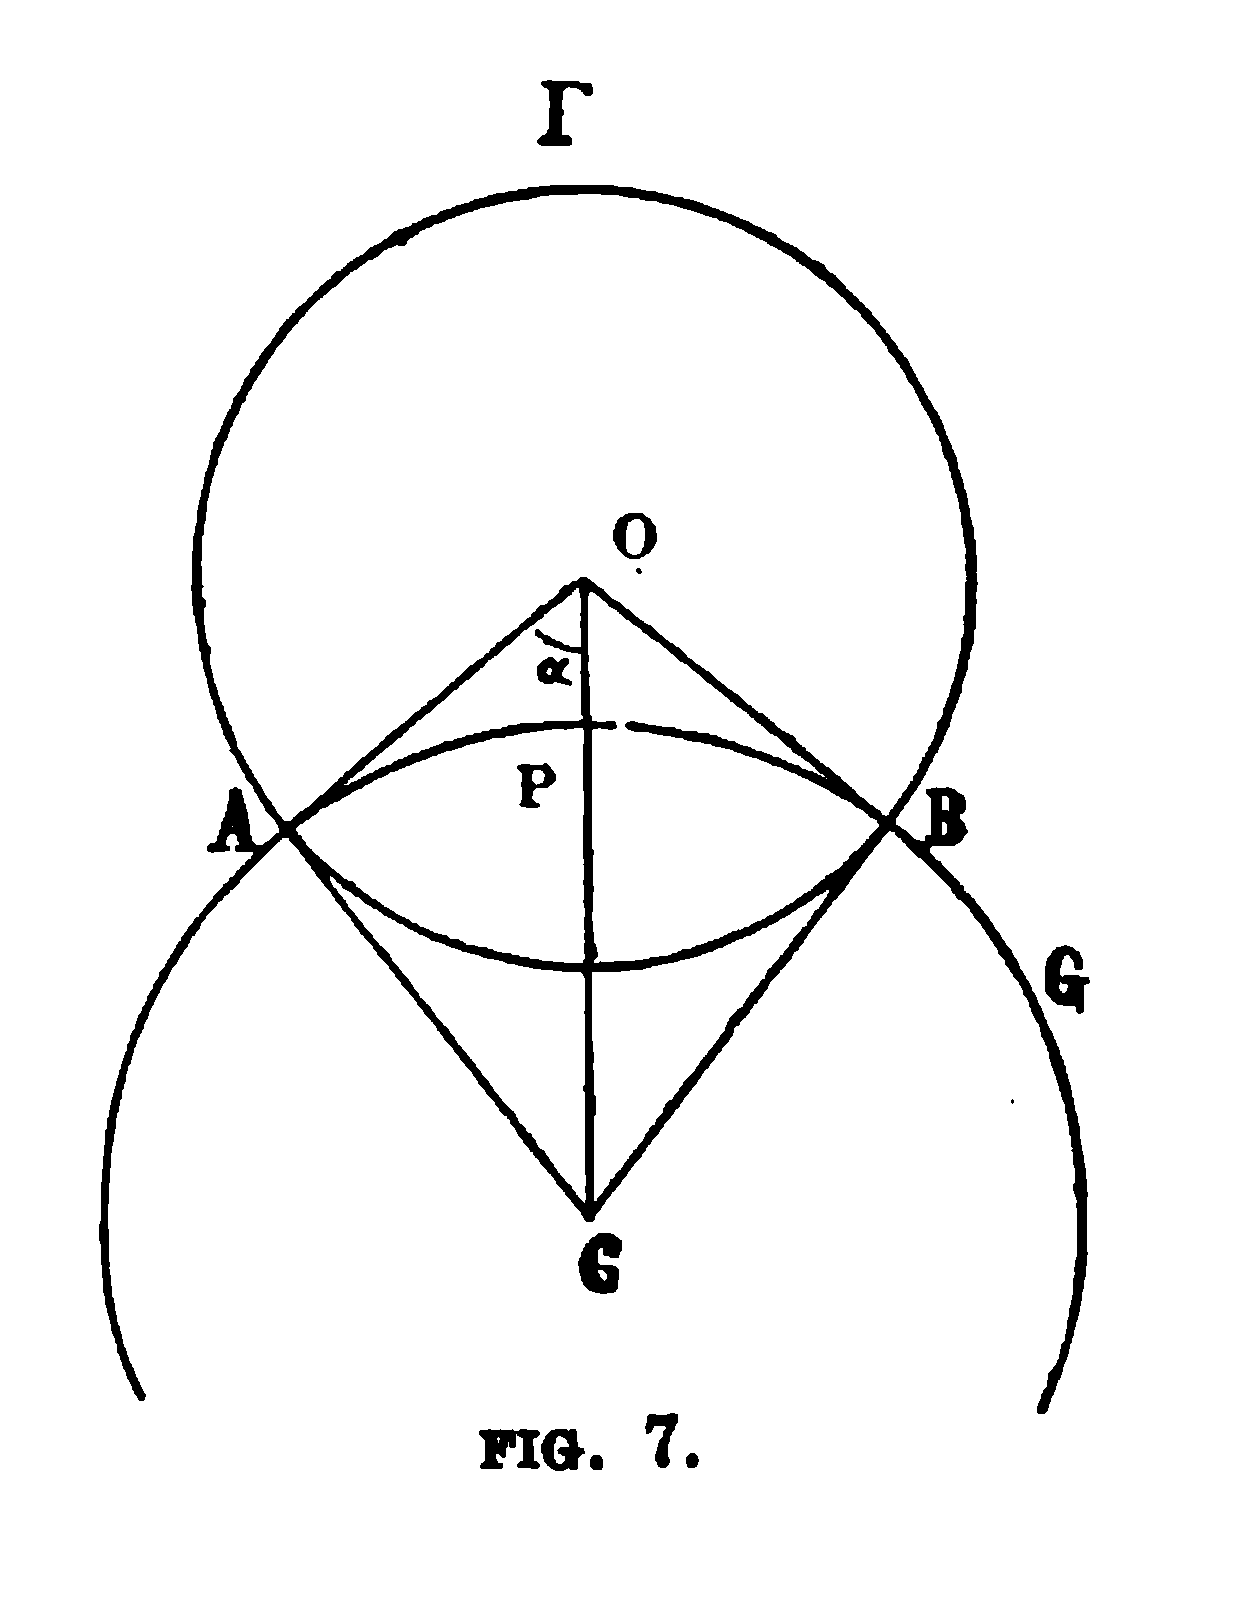
\includegraphics[width=.34\textwidth]{assets/ch12_figures/Luigi_Bianchi_Geometria_differenziale_Figura_7_facsimile.png}\end{center}}
\newcommand{\figsevena}{%
\begin{center}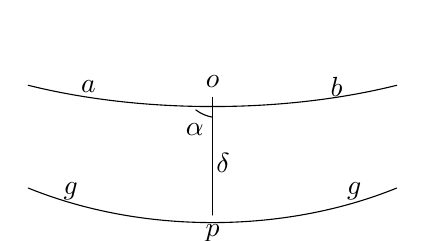
\begin{tikzpicture}[scale=0.9,line cap=round,line join=round]
\draw (-2.6,.65) .. controls (-1,.25) and (1,.25) .. (2.6,.65);
\draw (-2.6,-.8) .. controls (-1,-1.45) and (1,-1.45) .. (2.6,-.8);
\draw (0,.48)--(0,-1.18); \node[above] at (0,.48) {$o$}; \node[below] at (0,-1.18) {$p$};
\node at (-1.75,.63) {$a$}; \node at (1.75,.63) {$b$}; \node at (-2.0,-.85) {$g$}; \node at (2.0,-.85) {$g$};
\draw (0,.2) arc (260:233:.55); \node at (-.25,.03) {$\alpha$}; \node at (.15,-.45) {$\delta$};
\end{tikzpicture}\\[-.2em]{\small Fig. 7a.}\end{center}}
\newcommand{\figeight}{%
\begin{center}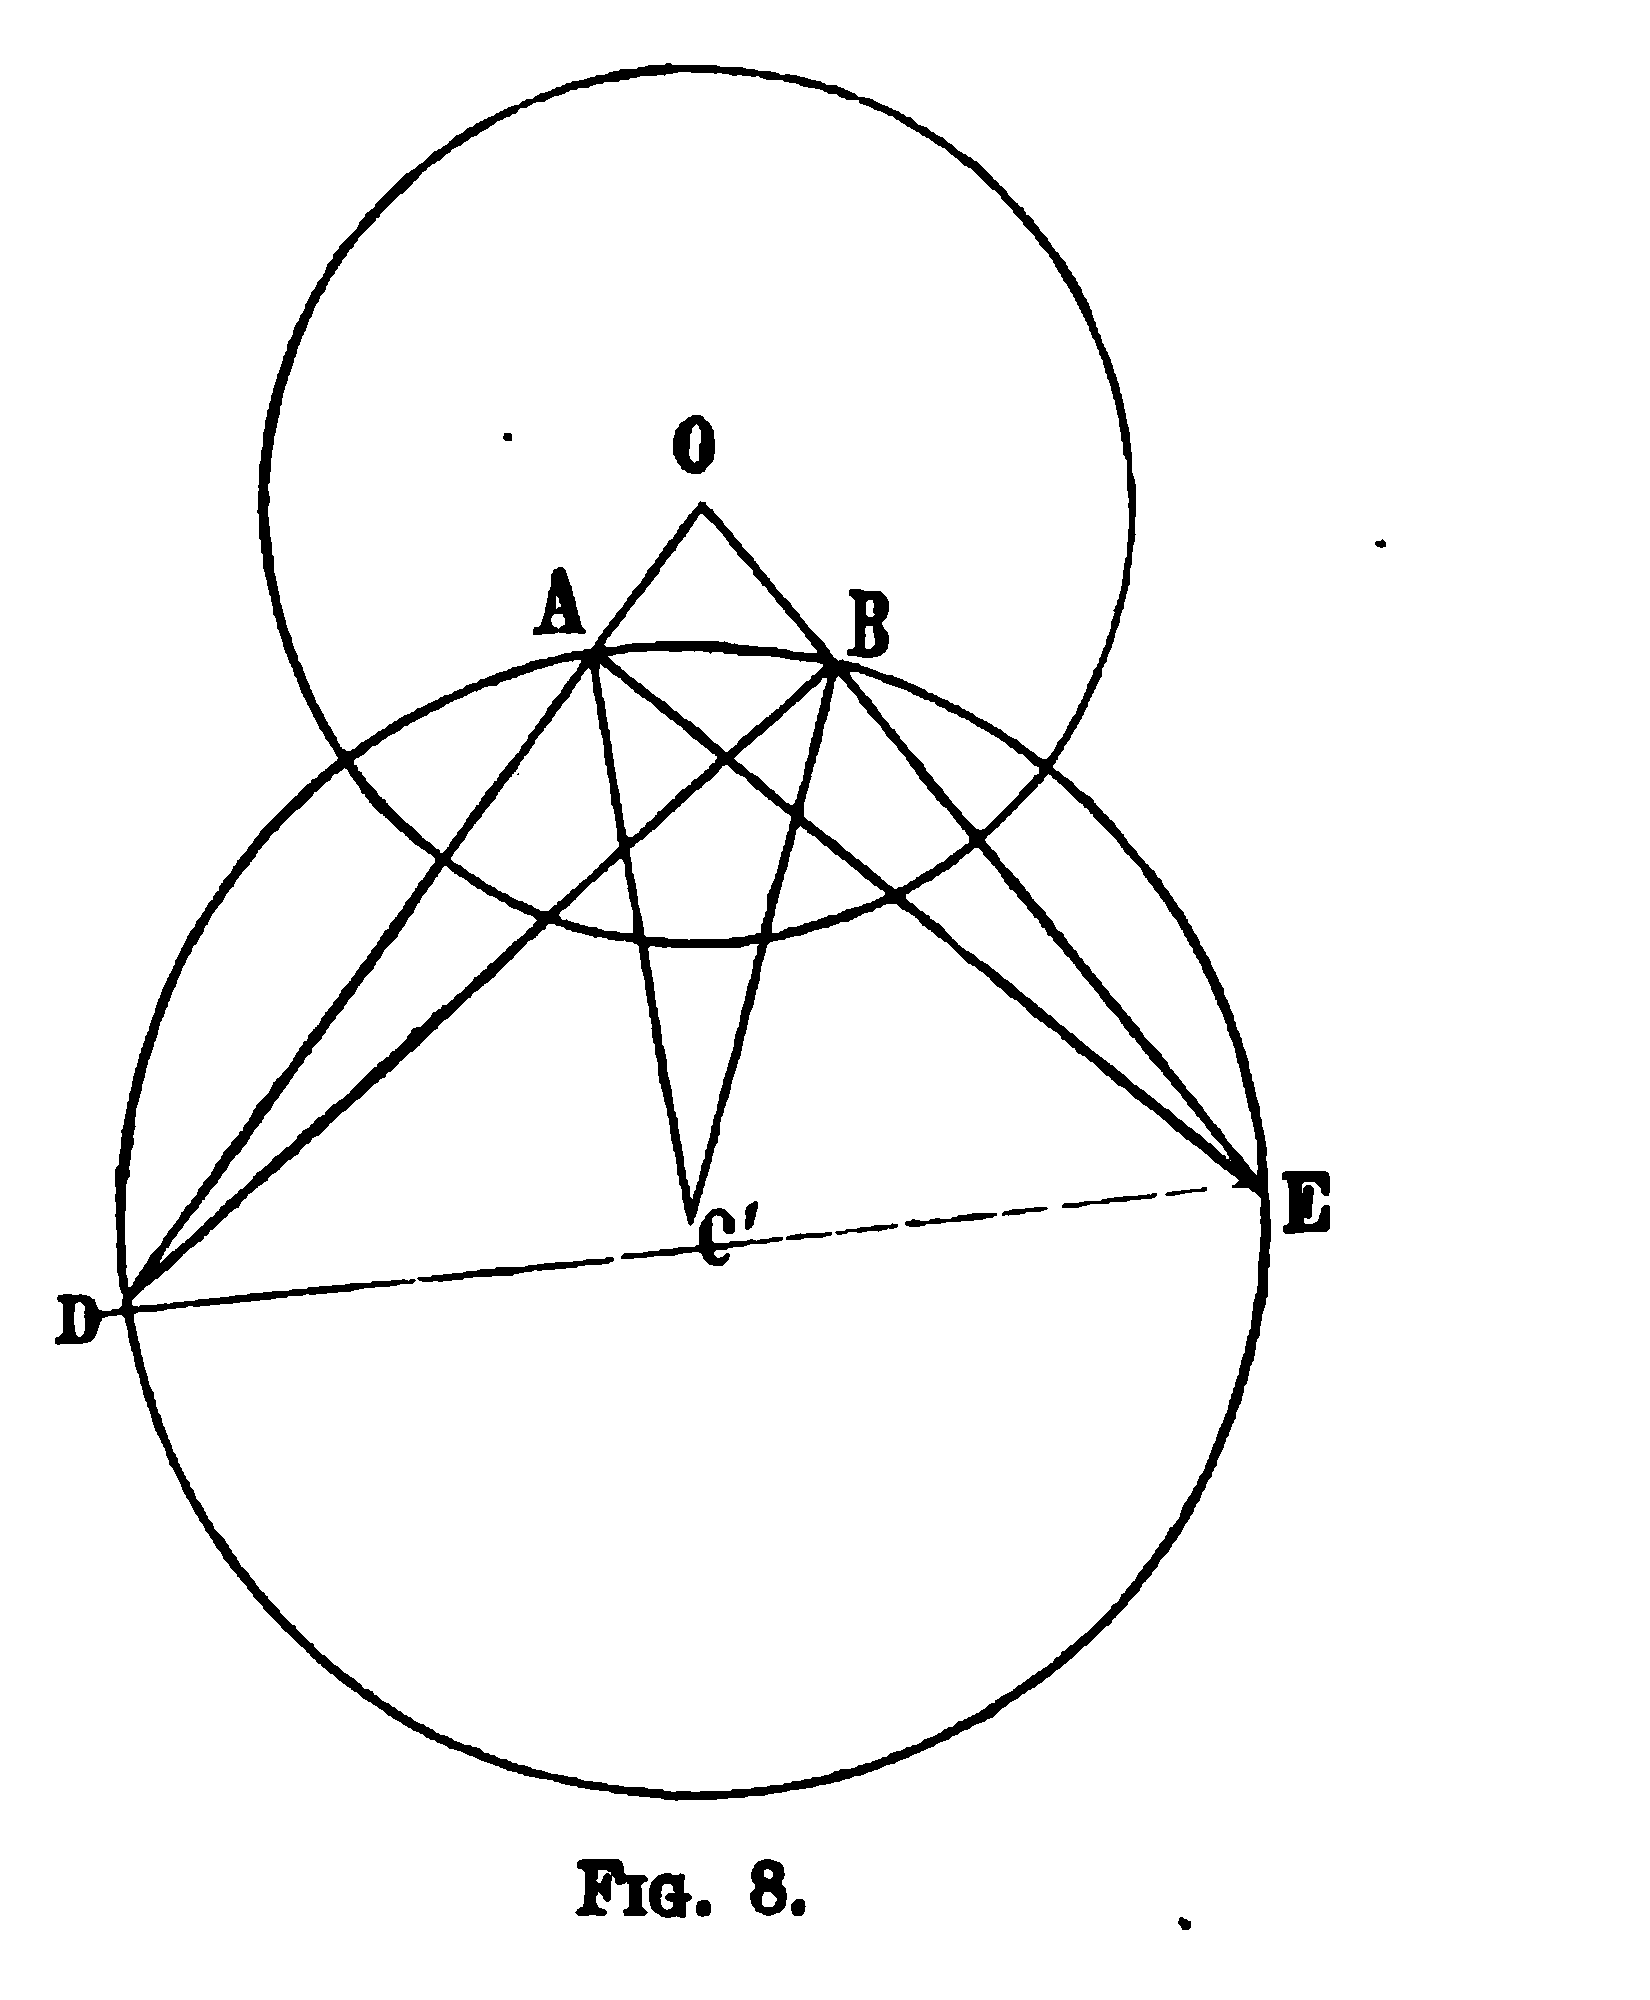
\includegraphics[width=.33\textwidth]{assets/ch12_figures/Luigi_Bianchi_Geometria_differenziale_Figura_8_facsimile.png}\end{center}}
\newcommand{\fignine}{%
\begin{center}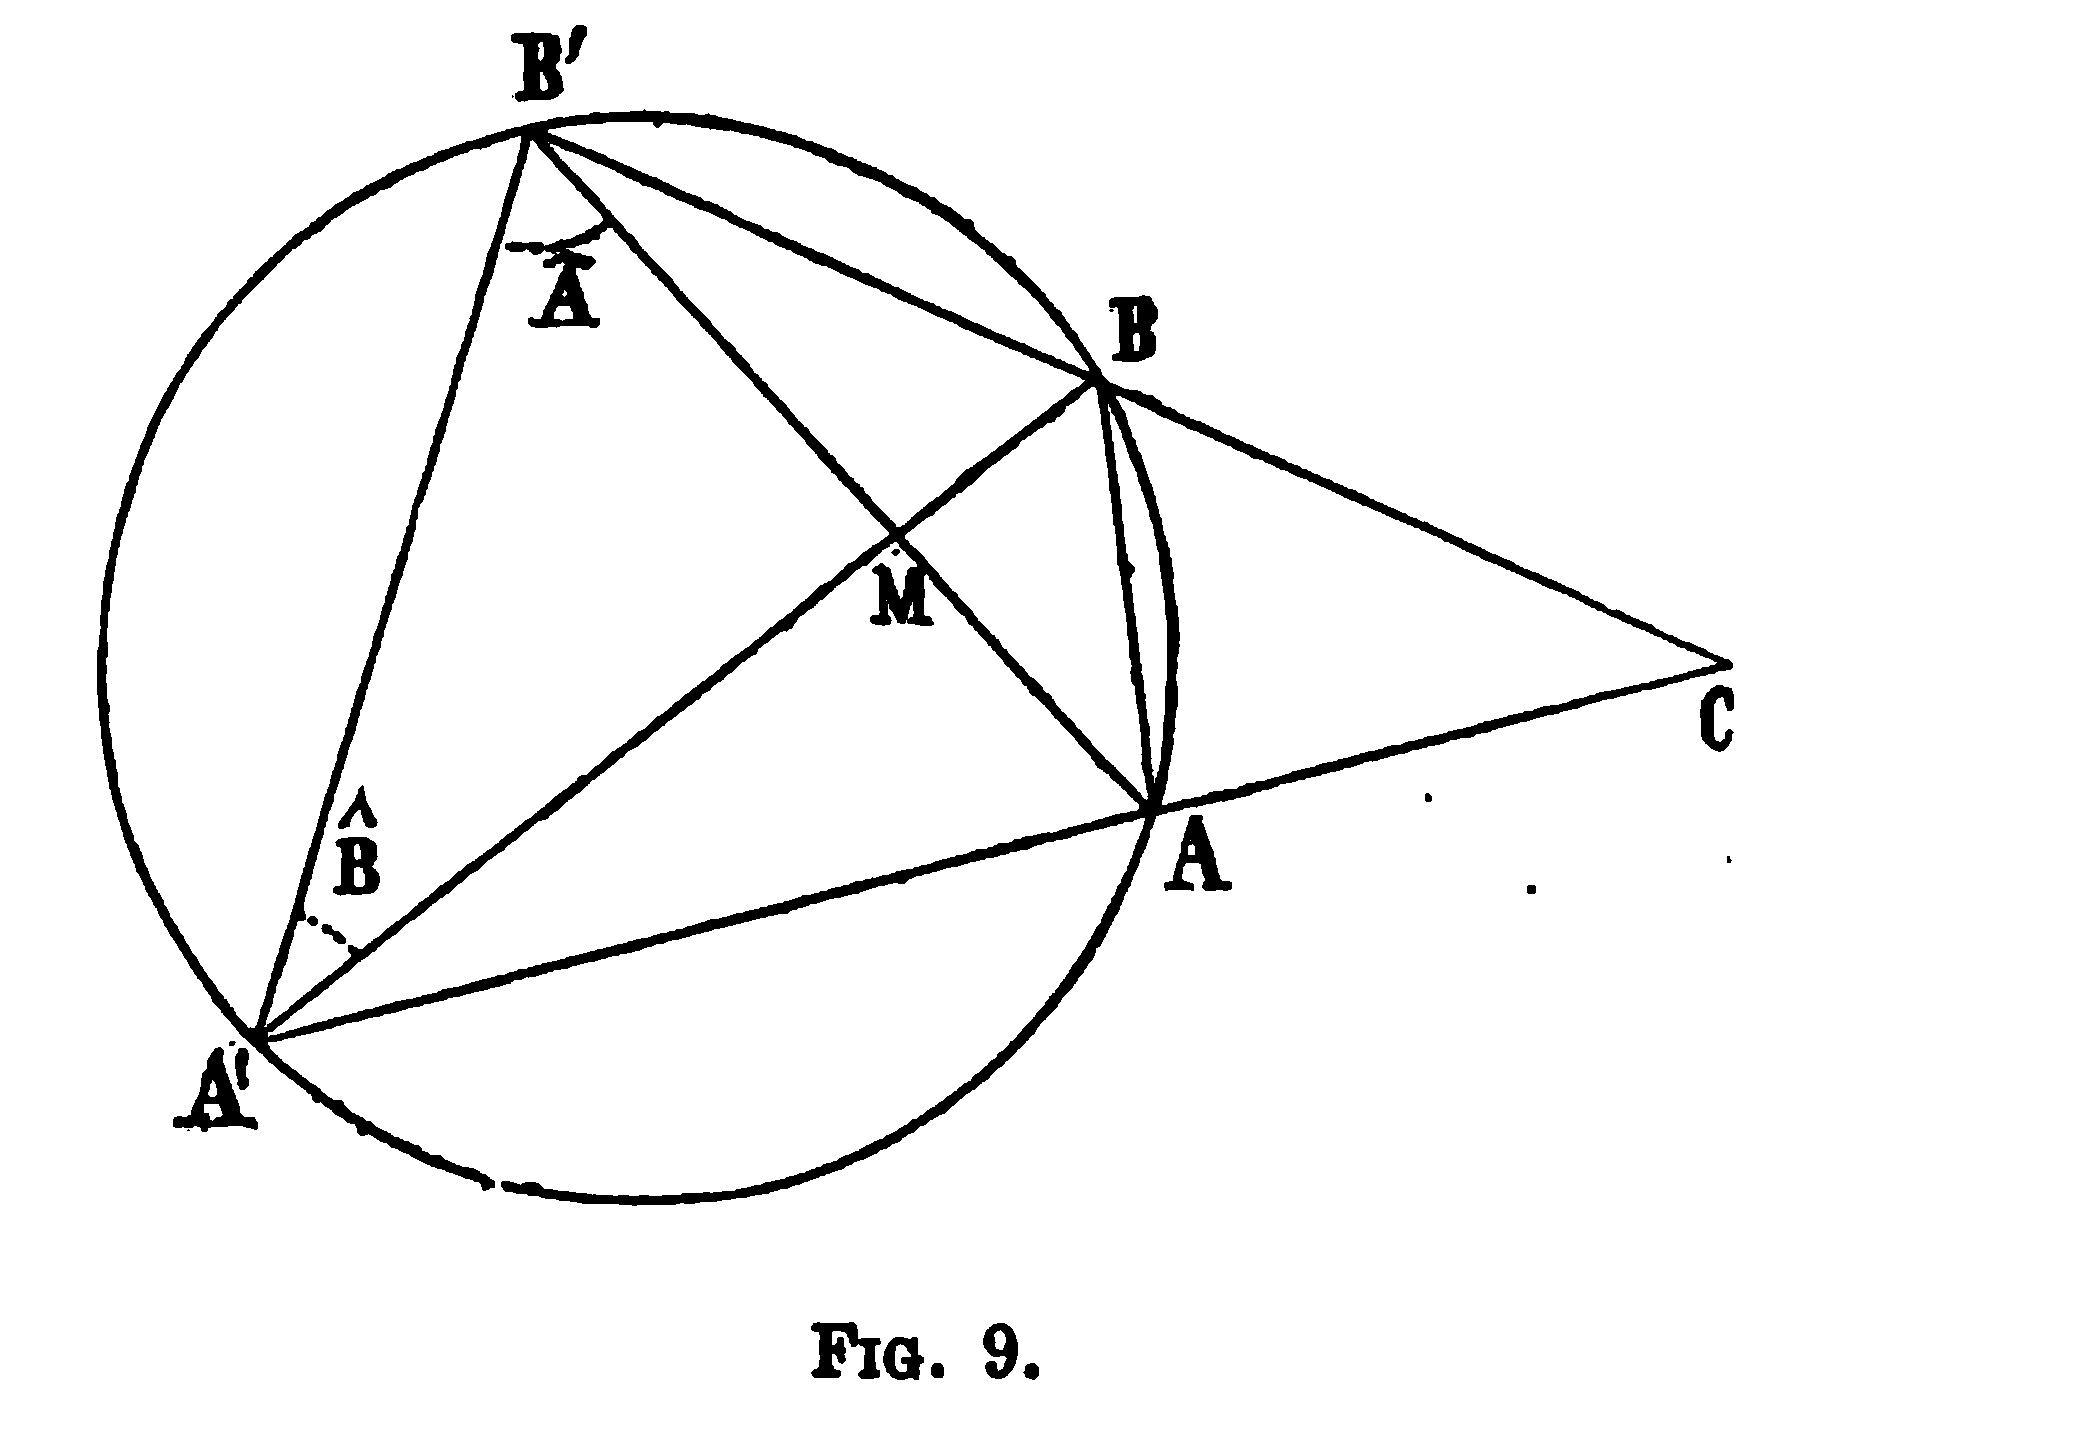
\includegraphics[width=.43\textwidth]{assets/ch12_figures/Luigi_Bianchi_Geometria_differenziale_Figura_9_facsimile.png}\end{center}}


% compatibility shims for p0409--0440 continuation
\providecommand{\sen}{\operatorname{sen}}
\providecommand{\tg}{\operatorname{tg}}
\providecommand{\senh}{\operatorname{senh}}
\providecommand{\tgh}{\operatorname{tgh}}
\providecommand{\cotgh}{\operatorname{cotgh}}
\providecommand{\ang}{\operatorname{ang}}
\providecommand{\grad}{\operatorname{grad}}
\providecommand{\chrB}[2]{\left\{\begin{matrix}#1\\#2\end{matrix}\right\}}
\providecommand{\chrsqB}[2]{\left[\begin{matrix}#1\\#2\end{matrix}\right]}


\ifLuaTeX
  \pdfextension info {
    /Title (Luigi Bianchi - Lectures on Differential Geometry, Volume I - Simplified Chinese)
    /Subject (Complete cumulative Simplified-Chinese reader edition)
    /Author (Luigi Bianchi)
  }
\fi

% Title matter carries the sole \begin{document}.
%% UNIT title | IT authority lines 129--155
\begin{document}

\thispagestyle{empty}

\begin{center}
{\bfseries 路易吉·比安基（LUIGI BIANCHI）}\par
{\small 比萨皇家大学教授}\par
\vspace{1.5em}
{\Huge\bfseries 讲义}\par
\vspace{1em}
关于\par
\vspace{1em}
{\LARGE\bfseries 微分几何}\par
\vspace{1em}
修订并大幅增补的第二版\par
{\bfseries 全二卷}\par
\vspace{1.25em}
{\large\bfseries 第一卷}\par
\vspace{4em}
{\large 比萨}\par
{\bfseries 恩里科·斯波埃里}\par
{\scriptsize 书商兼出版者}\par
1902
\end{center}

\begin{center}
{\small 比萨，尼斯特里兄弟继承人印刷所，1902年}
\end{center}

\clearpage

%% UNIT preface | IT authority lines 156--188
\pagenumbering{roman}
\section*{序言}
本书第二版的出版既已显得适宜，我认为，在保留全书基本构想的同时，最好大幅扩充其篇幅，使先前因篇幅过于狭窄而不得不压缩的许多理论部分，能够在新的论述中得到更为充分的发展。我还增添了若干新章：一方面用以论述那些虽已相当久远、却未能收入第一版的理论；另一方面用以介绍年代极近的研究，因为这些研究看来标志着无穷小几何在最近时期所取得的最重要进展。

本书的篇幅由此增加到原来的两倍，因而必须分为两卷；我力求使这种分卷大体上与一般理论和特殊理论的区分相对应。

本第一卷共有十四章。其中前十章在作了许多改动和增补之后，重现第一版相应各章的内容；我还从第一版录取如下说明。

\oldquote
“本课程所完全遵循的方法，发端于高斯著名的\emph{《曲面的一般研究》（Disquisitiones generales circa superficies curvas）》}；这一方法把无穷小几何看作对一个二次微分形式、或者同时对两个这样的形式所作的研究。因此，在论述双曲率曲线的第一章之后，读者将在第二章看到二次微分形式理论的基础；那里只作极为简要的陈述。
\closeoldquote

\oldquote
由这一理论产生的算法具有一项重大优点：它们在完全保留坐标线一般性的同时，使公式呈现出简洁优美、易于记忆的形式。本书后文始终使用这些算法，而本章正是其预备章节。

随后七章（第三至第九章）论述曲面的一般研究，也就是说，既研究曲面在空间中的实际形状所固有的性质，又研究那些在曲面弯曲时保持不变的性质（等距适用性理论）。第十章论述射线的二重无穷系统（直线汇）的一般理论；这一理论对于曲面的一般研究极为重要，无穷小几何的许多最卓越成果也由此而来。”
\closeoldquote

以下四章以更充分的展开和大量增补，重新呈现我曾在本书德文版\footnote{\emph{Vorlesungen über Differentialgeometrie}，M. Lukat 德译（Teubner，莱比锡，1899年）。}中给出的 \(n\) 维无穷小几何基本原理。第十一章先为任意 \(n\) 维空间的线度量和角度量规定基本约定，继而引入黎曼曲率的概念，并把通常理论中的公式推广到曲线和超曲面，尤其着重研究曲率线的性质。

然后我较为专门地研究具有常黎曼曲率的空间。首先在第十二章（相当于第一版的第十六章）讨论二维伪球几何，并对非欧几何作一简短说明。

在接下来的第十三章中，我一般地研究具有常曲率的 \(n\) 维空间，引入凯莱度量和魏尔斯特拉斯坐标系，并特别研究三维空间中运动的解析表示及其性质；最后讨论椭圆空间中重要的克利福德平行性概念，以及如何把曲线的弗雷内公式推广到椭圆几何和双曲几何。

最后，第十四章把这些一般理论应用于具有常曲率的 \(n\) 维空间中的超曲面，特别关注三维情形；在这一情形下，欧氏空间中已有的全部主要结果都得到推广。

我的同事 O. Niccoletti 教授\ednote{印本姓名拼作 ``Niccoletti''（双写 c）；继承的意大利文与英文转录曾无说明地写作 ``Nicoletti''。本简体中文版按印本恢复 ``Niccoletti''。}曾热心协助我完成校样的最后一次审订，谨在此向他致以最诚挚的谢意。

\begin{flushleft}
\emph{比萨，1902年4月。}
\end{flushleft}

\clearpage
\pagenumbering{arabic}


% Chapter I.
%% UNIT ch01_s01_s03 | IT authority lines 189--341
\section*{第一章}
\begin{center}
{\Large\bfseries 双曲率曲线}
\end{center}

\begin{center}\footnotesize
切线与法平面。-- 第一曲率或弯曲率。-- 密切平面。-- 主三面形。-- 第二曲率或挠率。-- 弗雷内公式。-- 内蕴方程。-- 柱面螺线。-- 包络面。-- 管状面。-- 可展曲面。-- 曲线的矫直可展面与极可展面。-- 极可展面的回归棱。-- 渐开线与渐屈线。-- 单参数平面族的正交轨迹。-- Combescure 变换。-- 第一曲率为常数的曲线与球面螺线。-- 单参数球面族的正交轨迹。-- 贝特朗曲线。
\end{center}

\subsection*{§. 1.\quad 切线与法平面}
为了用解析方法定义曲线 \(C\)，我们把它参照于一组正交笛卡儿坐标轴 \(Ox, Oy, Oz\)，并把曲线上动点的坐标 \(x,y,z\) 表示为参数 \(u\) 的函数：
\[
  x=x(u), \qquad y=y(u), \qquad z=z(u).
\]
关于函数 \(x(u),y(u),z(u)\)，我们在此一劳永逸地约定：在独立变量 \(u\) 的整个定义区间内，除至多若干特殊点外，\emph{这些函数连同其一阶、二阶和三阶导数均为有限且连续的}。

在所考察的区间内，每一个特定值 \(u_1\)，当把它赋给参数 \(u\) 时，都对应于曲线生成点的一个特定位置 \(M_1\)，这个生成点记为 \(M\)。当 \(u\) 连续变化时，点 \(M\) 依连续规律在空间中运动，从而描出曲线 \(C\)。我们还始终约定：生成点 \(M\) 在参数 \(u\) 增大时的运动方向，取为曲线 \(C\) 的正向；相反方向则为负向。

多数情况下，我们取作参数或辅助变量 \(u\) 的是弧长 \(s\)，即曲线 \(C\) 的弧长；它从一个固定点（原点）起算。无论如何，为了把 \(s\) 定义成 \(u\) 的函数，我们有熟知的

\noindent 公式：
\[
\frac{\diff s}{\diff u}=\sqrt{\left(\frac{\diff x}{\diff u}\right)^2+\left(\frac{\diff y}{\diff u}\right)^2+\left(\frac{\diff z}{\diff u}\right)^2},
\]
其中，既然规定 \(s\) 沿 \(u\) 增大的方向计量，根式就必须取正号。

在一点 \(M\) 处考虑曲线 \(C\) 的切线，并规定其正向与曲线的正向一致。此后我们将始终用 \(\alpha,\beta,\gamma\) 表示这条切线正向的方向余弦，于是有公式：
\[
\alpha=\frac{\dfrac{\diff x}{\diff u}}{\sqrt{\left(\dfrac{\diff x}{\diff u}\right)^2+\left(\dfrac{\diff y}{\diff u}\right)^2+\left(\dfrac{\diff z}{\diff u}\right)^2}},\qquad
\beta=\frac{\dfrac{\diff y}{\diff u}}{\sqrt{\left(\dfrac{\diff x}{\diff u}\right)^2+\left(\dfrac{\diff y}{\diff u}\right)^2+\left(\dfrac{\diff z}{\diff u}\right)^2}},
\]
\[
\gamma=\frac{\dfrac{\diff z}{\diff u}}{\sqrt{\left(\dfrac{\diff x}{\diff u}\right)^2+\left(\dfrac{\diff y}{\diff u}\right)^2+\left(\dfrac{\diff z}{\diff u}\right)^2}},
\]
或者
\begin{equation}\tag{1}
\alpha=\frac{\diff x}{\diff s},\qquad \beta=\frac{\diff y}{\diff s},\qquad \gamma=\frac{\diff z}{\diff s}.
\end{equation}
在公式 (1) 中，把右端看成微分之商，或者看成对弧长所取的导数，二者并无区别。

在 \(M\) 处与切线垂直的平面称为曲线的法平面；以 \(X,Y,Z\) 表示动点的坐标，它的方程为
\[
(X-x)\alpha+(Y-y)\beta+(Z-z)\gamma=0,
\]

\subsection*{§. 2.\quad 第一曲率或弯曲率}
曲线生成点偏离直线方向的快慢，使我们判断曲线本身的\emph{弯曲率}较大还是较小。为了精确规定这一概念并使之可以度量，取曲线的一点 \(M\) 和一个邻近点 \(M_1\)。两条切线方向所成的极小角记为 \(\Delta\varepsilon\)，这里的切线分别取在 \(M,M_1\) 处；把这个角除以弧长 \(MM_1=\Delta s\)。商 \(\Delta\varepsilon/\Delta s\) 在 \(M_1\) 无限趋近于 \(M\) 时（即 \(\Delta s\) 趋于零）趋于一个确定的有限极限；我们取这个极限作为曲线在 \(M\) 处的\emph{第一曲率或弯曲率}的度量。以 \(1/\rho\) 表示该极限；其倒数 \(\rho\) 被解释为长度，称为\emph{第一曲率半径}。

为了证明这一极限存在并同时求出它的表达式，我们采用如下考察。

以原点为球心、以单位长度为半径作一球面，并用此球面截取那些分别平行于曲线各相继切线正向的射线。这些射线端点的轨迹称为切线的\emph{球面指标曲线}。生成点 \(M=(x,y,z)\) 在曲线 \(C\) 上的每一个位置，都对应于一点 \(M'=(x',y',z')\)，该点位于切线的球面指标曲线 \(C'\) 上；显然有
\begin{equation}\tag{2}
x'=\alpha,\qquad y'=\beta,\qquad z'=\gamma.
\end{equation}
现在取一点 \(M_1\)，它在曲线 \(C\) 上邻近 \(M\)。角 \(\Delta\varepsilon\) 恰由表示球面上连接像点 \(M',M'_1\) 的大圆弧来度量。为了计算极限
\[
\frac{1}{\rho}=\lim_{\Delta s\to0}\left(\frac{\Delta\varepsilon}{\Delta s}\right),
\]
可以用指标曲线上相应的弧代替 \(\Delta\varepsilon\)：当 \(\Delta s\) 趋于零时，这条弧是无穷小量，而它与 \(\Delta\varepsilon\) 的比趋于一。以 \(\diff s'\) 表示球面指标曲线的弧微元，于是立即得到
\[
\frac{1}{\rho}=\frac{\diff s'}{\diff s},
\]
或者由 (2) 得
\begin{equation}\tag{3}
\frac{1}{\rho}=\sqrt{\left(\frac{\diff\alpha}{\diff s}\right)^2+\left(\frac{\diff\beta}{\diff s}\right)^2+\left(\frac{\diff\gamma}{\diff s}\right)^2}.
\end{equation}

若取 \(s\) 为独立变量，利用 (1)，该公式可写成
\begin{equation}\tag{3*}
\frac{1}{\rho}=\sqrt{\left(\frac{\diff^2x}{\diff s^2}\right)^2+\left(\frac{\diff^2y}{\diff s^2}\right)^2+\left(\frac{\diff^2z}{\diff s^2}\right)^2}.
\end{equation}
在这些公式中，\emph{我们约定第一曲率只取绝对值}，因而总是取根式的正值。

立即可以看出，曲线 \(C\) 不可能在某一\emph{曲线段}上弯曲率处处为零而该段却不是直线。事实上，由随之而来的方程
\[
\frac{\diff\alpha}{\diff s}=0,\qquad \frac{\diff\beta}{\diff s}=0,\qquad \frac{\diff\gamma}{\diff s}=0,
\]
可知 \(\alpha,\beta,\gamma\) 均为常数，于是有
\[
x=\alpha s+a,\qquad y=\beta s+b,\qquad z=\gamma s+c,
\]
其中 \(a,b,c\) 为常数；这些公式定义一条直线。

\subsection*{§. 3.\quad 密切平面}
在所有通过一点 \(M\) 的平面中——这里说的是曲线 \(C\) 上的一点——有一个平面在 \(M\) 的邻域内比任何其他平面偏离曲线 \(C\) 都更少；它称为曲线在 \(M\) 处的\emph{密切平面}。事实上，把通过 \(M=(x,y,z)\) 的任意平面方程写成
\begin{equation}\tag{4}
a(X-x)+b(Y-y)+c(Z-z)=0,
\end{equation}
其中 \(a,b,c\) 是该平面法线的方向余弦。取参数 \(u\) 为曲线的弧长 \(s\)，并考虑一点 \(M'\)，它邻近 \(M\)，且对应于弧长值 \(s+h\)，其中 \(h\) 被看作一阶无穷小量。若 \(\Delta x,\Delta y,\Delta z\) 是 \(x,y,z\) 从 \(s\) 变到 \(s+h\) 时的相应增量，则距离 \(\delta\)，也就是点 \(M'\) 到平面 (4) 的距离，满足
\[
\delta=a\Delta x+b\Delta y+c\Delta z.
\]

现在有
\begin{equation}\tag{a}
\left\{
\begin{aligned}
\Delta x&=\frac{\diff x}{\diff s}h+\frac{\diff^2x}{\diff s^2}\frac{h^2}{2}+\varepsilon_1,\\
\Delta y&=\frac{\diff y}{\diff s}h+\frac{\diff^2y}{\diff s^2}\frac{h^2}{2}+\varepsilon_2,\\
\Delta z&=\frac{\diff z}{\diff s}h+\frac{\diff^2z}{\diff s^2}\frac{h^2}{2}+\varepsilon_3,
\end{aligned}
\right.
\end{equation}
其中 \(\varepsilon_1,\varepsilon_2,\varepsilon_3\) 是\emph{三阶}无穷小量，因而
\[
\delta=\left(a\frac{\diff x}{\diff s}+b\frac{\diff y}{\diff s}+c\frac{\diff z}{\diff s}\right)h+
\left(a\frac{\diff^2x}{\diff s^2}+b\frac{\diff^2y}{\diff s^2}+c\frac{\diff^2z}{\diff s^2}\right)\frac{h^2}{2}+\eta,
\]
其中 \(\eta\) 是三阶无穷小量。

由条件
\[
a\frac{\diff x}{\diff s}+b\frac{\diff y}{\diff s}+c\frac{\diff z}{\diff s}=0,
\]
\[
a\frac{\diff^2x}{\diff s^2}+b\frac{\diff^2y}{\diff s^2}+c\frac{\diff^2z}{\diff s^2}=0,
\]
确定的平面，就是在 \(M\) 的邻域内比其他平面偏离曲线更少的那个平面；第一个条件表示该平面包含切线。这样，我们已经证明了密切平面的存在。根据以上结果，它的方程可以写成如下行列式形式\footnote{即使采用任意独立变量 \(u\)，密切平面的方程显然仍保持同一形式：
\[
\detmat{X-x & Y-y & Z-z\\ x' & y' & z'\\ x'' & y'' & z''}=0,
\]
其中撇号表示对 \(u\) 求导。}：
\begin{equation}\tag{5}
\detmat{X-x & Y-y & Z-z\\
\dfrac{\diff x}{\diff s} & \dfrac{\diff y}{\diff s} & \dfrac{\diff z}{\diff s}\\
\dfrac{\diff^2x}{\diff s^2} & \dfrac{\diff^2y}{\diff s^2} & \dfrac{\diff^2z}{\diff s^2}}=0.
\end{equation}

曲线在一点 \(M\) 处的密切平面一般是唯一且确定的。

唯一的例外，是下列矩阵的三个二阶子式同时为零的那些点：
\[
\left\|\begin{matrix}
\dfrac{\diff x}{\diff s} & \dfrac{\diff y}{\diff s} & \dfrac{\diff z}{\diff s}\\
\dfrac{\diff^2x}{\diff s^2} & \dfrac{\diff^2y}{\diff s^2} & \dfrac{\diff^2z}{\diff s^2}
\end{matrix}\right\|.
\]
但是，由于公式
\[
\left(\frac{\diff x}{\diff s}\right)^2+\left(\frac{\diff y}{\diff s}\right)^2+\left(\frac{\diff z}{\diff s}\right)^2=1,
\]
\[
\frac{\diff x}{\diff s}\frac{\diff^2x}{\diff s^2}+\frac{\diff y}{\diff s}\frac{\diff^2y}{\diff s^2}+\frac{\diff z}{\diff s}\frac{\diff^2z}{\diff s^2}=0,
\]
这个矩阵的平方由 (3*) 等于弯曲率的平方，所以可见，上述奇点正是弯曲率为零的点。

我们还要提及密切平面的另外一些定义；不难看出，它们总是导出方程 (5)。

通过 \(M\) 处的切线和一个邻近点 \(M'\) 作一平面，其中该点属于曲线 \(C\)；当 \(M'\) 趋于 \(M\) 时，该平面作为极限平面趋于密切平面。又，通过 \(M\) 和另外两个邻近点 \(M',M''\) 作一平面；当 \(M',M''\) 同时趋于 \(M\) 时，该平面趋于密切平面（这里要求 \(M',M''\) 两点相应坐标之差，不成为比它们各自与 \(M\) 的相应坐标之差更高阶的无穷小量）。根据最后这一性质，也可以简略地说：一点处的密切平面，就是通过该点和曲线上继后的两个点所作的平面。

%% UNIT ch01_s04_s06 | IT authority lines 342--525
\subsection*{§. 4.\quad 主三面形}
在曲线于 \(M\) 处的所有法线中，位于密切平面内的那一条称为\emph{主法线}，也就是密切平面与法平面的交线。密切平面的法线则称为曲线的\emph{副法线}。

我们已经规定了切线的正向；现在还须借助适当的约定，规定主法线和副法线的正向。这三个正向确定一个三直角三面形，我们称之为曲线在所考察点 \(M\) 处的\emph{主三面形}。

以下始终以
\[
\xi,\ \eta,\ \zeta
\]
表示主法线（正向）的方向余弦，并以
\[
\lambda,\ \mu,\ \nu
\]
表示副法线的方向余弦。由密切平面的方程 (5) 立即得到比例式
\[
\lambda:\mu:\nu=
\detmat{\dfrac{\diff y}{\diff s} & \dfrac{\diff z}{\diff s}\\[0.6em]
\dfrac{\diff^2y}{\diff s^2} & \dfrac{\diff^2z}{\diff s^2}}
:
\detmat{\dfrac{\diff z}{\diff s} & \dfrac{\diff x}{\diff s}\\[0.6em]
\dfrac{\diff^2z}{\diff s^2} & \dfrac{\diff^2x}{\diff s^2}}
:
\detmat{\dfrac{\diff x}{\diff s} & \dfrac{\diff y}{\diff s}\\[0.6em]
\dfrac{\diff^2x}{\diff s^2} & \dfrac{\diff^2y}{\diff s^2}},
\]
因而（由于 \(\xi\alpha+\eta\beta+\zeta\gamma=0,\ \xi\lambda+\eta\mu+\zeta\nu=0\)）：
\[
\xi:\eta:\zeta=\frac{\diff^2x}{\diff s^2}:\frac{\diff^2y}{\diff s^2}:\frac{\diff^2z}{\diff s^2};
\]
所以由 (3*) 推得
\begin{equation}\tag{6}
\xi=\pm\rho\frac{\diff^2x}{\diff s^2},\qquad
\eta=\pm\rho\frac{\diff^2y}{\diff s^2},\qquad
\zeta=\pm\rho\frac{\diff^2z}{\diff s^2}.
\end{equation}
现在考虑由切线和副法线确定的平面，其方程为
\begin{equation}\tag{7}
(X-x)\xi+(Y-y)\eta+(Z-z)\zeta=0,
\end{equation}
并计算有向距离 \(\delta\)：它是曲线上一点 \(M'\) 到这个平面的距离，而该点邻近 \(M\)。沿用 §. 3 的记号，有
\[
\delta=\xi\Delta x+\eta\Delta y+\zeta\Delta z,
\]
由解析几何所熟知，\(\delta\) 的正负取决于 \(M'\) 位于平面 (7) 的正侧还是负侧，也就是说，位于该平面法线正向

\noindent \((\xi,\eta,\zeta)\) 所指的区域，还是相反的区域。现在应用第5页的公式 (a)，并注意 (6)，得到
\begin{equation}\tag{8}
\delta=\pm\frac{h^2}{2\rho}+\eta,
\end{equation}
这里的 \(\eta\) 表示一个三阶无穷小量。由此式可见，\(\delta\) 的符号与 \(h\) 的符号无关，因而：\emph{在曲线每一点的邻域内，曲线完全位于由切线和副法线所成平面的同一侧}\footnote{须排除弯曲率为零的奇点。}。我们把该平面在 \(M\) 的邻域内朝向曲线的一侧定为正侧；这样也就规定了主法线的正向。根据这一约定，(8) 中的 \(\delta\) 应为正，因此 (6) 中必须取上面的符号。于是得到最后的公式
\begin{equation}\tag{9}
\xi=\rho\frac{\diff^2x}{\diff s^2},\qquad
\eta=\rho\frac{\diff^2y}{\diff s^2},\qquad
\zeta=\rho\frac{\diff^2z}{\diff s^2}.
\end{equation}
最后，我们约定副法线的正向 \((\lambda,\mu,\nu)\)：它相对于已经规定的切线与主法线的正向，正如 \(Oz\) 轴的正向相对于 \(Ox,Oy\) 两轴的正向。三个主方向的九个方向余弦所成的行列式
\[
\detmat{\alpha & \beta & \gamma\\
\xi & \eta & \zeta\\
\lambda & \mu & \nu}
\]
等于正一，并且其中每个元素都等于它自己的代数余子式。因此有
\begin{equation}\tag{10}
\left\{
\begin{aligned}
\lambda&=\beta\zeta-\gamma\eta=\rho\left(\frac{\diff y}{\diff s}\frac{\diff^2z}{\diff s^2}-\frac{\diff z}{\diff s}\frac{\diff^2y}{\diff s^2}\right),\\[0.4em]
\mu&=\gamma\xi-\alpha\zeta=\rho\left(\frac{\diff z}{\diff s}\frac{\diff^2x}{\diff s^2}-\frac{\diff x}{\diff s}\frac{\diff^2z}{\diff s^2}\right),\\[0.4em]
\nu&=\alpha\eta-\beta\xi=\rho\left(\frac{\diff x}{\diff s}\frac{\diff^2y}{\diff s^2}-\frac{\diff y}{\diff s}\frac{\diff^2x}{\diff s^2}\right).
\end{aligned}\right.
\end{equation}

\subsection*{§. 5.\quad 第二曲率或挠率}
曲线 \(C\) 的密切平面一般随密切点 \(M\) 的变化而变化；它偏转的快慢，也就是曲线偏离平面状态的快慢，用\emph{第二曲率或挠率}来度量。

为了同样精确地规定这一概念，取曲线的一点 \(M\) 及其邻近点 \(M_1\)。\(M,M_1\) 两点处的密切平面夹一个极小角 \(\Delta\sigma\)。商 \(\Delta\sigma/\Delta s\) 中，\(\Delta s\) 表示弧 \(MM_1\)；当 \(\Delta s\) 趋于零时，这个商趋于一个确定的有限极限。该极限被取作曲线\emph{挠率}的度量，并在赋予适当符号后记为 \(1/T\)。其倒数 \(T\) 称为第二曲率半径。为了求 \(1/T\) 的表达式，先注意角 \(\Delta\sigma\) 由 \(M,M_1\) 处两条相继副法线的夹角来度量。因此，完全仿照 §. 3 作出\emph{副法线的球面指标曲线}，其生成点的坐标为
\[
 x_1=\lambda,\qquad y_1=\mu,\qquad z_1=\nu,
\]
并以 \(\diff s_1\) 表示其弧微元
\[
\diff s_1=\sqrt{\diff x_1^2+\diff y_1^2+\diff z_1^2},
\]
显然有
\begin{equation}\tag{11}
\frac{1}{T}=\pm\frac{\diff s_1}{\diff s}=\pm\sqrt{\left(\frac{\diff\lambda}{\diff s}\right)^2+\left(\frac{\diff\mu}{\diff s}\right)^2+\left(\frac{\diff\nu}{\diff s}\right)^2}.
\end{equation}
下一节将以最便利的方式规定挠率的符号；这里先指出，挠率为零的曲线只有平面曲线。事实上，若 \(1/T=0\)，则由 (11) 可知 \(\lambda,\mu,\nu\) 是常数。为简便起见，若取副法线的固定方向为 \(z\) 轴，就有
\[
\lambda=0,
\qquad \mu=0,
\qquad \nu=1,
\]
从而 \(\gamma=0\)，所以 \(z=\) 常数；因此曲线位于一个平行于 \(xy\) 平面的平面内。

\subsection*{§. 6.\quad 弗雷内公式}
现在来建立一组重要公式：它们用三个主方向本身的九个方向余弦以及第一、第二曲率半径 \(\rho,T\)，表示这些方向余弦对弧长所取的导数。其中三个公式立即来自 §. 4（第8页）的 (9)，即
\begin{equation}\tag{a}
\frac{\diff\alpha}{\diff s}=\frac{\xi}{\rho},\qquad
\frac{\diff\beta}{\diff s}=\frac{\eta}{\rho},\qquad
\frac{\diff\gamma}{\diff s}=\frac{\zeta}{\rho}.
\end{equation}
现在把恒等式
\[
\alpha\lambda+\beta\mu+\gamma\nu=0,
\]
\[
\lambda^2+\mu^2+\nu^2=1,
\]
对 \(s\) 求导，并注意上面的 (a)，便得到
\[
\left\{
\begin{aligned}
\alpha\frac{\diff\lambda}{\diff s}+\beta\frac{\diff\mu}{\diff s}+\gamma\frac{\diff\nu}{\diff s}&=0,\\[0.4em]
\lambda\frac{\diff\lambda}{\diff s}+\mu\frac{\diff\mu}{\diff s}+\nu\frac{\diff\nu}{\diff s}&=0,
\end{aligned}\right.
\]
从而有比例式
\[
\frac{\diff\lambda}{\diff s}:\frac{\diff\mu}{\diff s}:\frac{\diff\nu}{\diff s}=
\detmat{\beta&\gamma\\ \mu&\nu}:
\detmat{\gamma&\alpha\\ \nu&\lambda}:
\detmat{\alpha&\beta\\ \lambda&\mu},
\]
也就是
\[
\frac{\diff\lambda}{\diff s}:\frac{\diff\mu}{\diff s}:\frac{\diff\nu}{\diff s}=\xi:\eta:\zeta.
\]
所以三个比
\[
\frac{1}{\xi}\frac{\diff\lambda}{\diff s},\qquad
\frac{1}{\eta}\frac{\diff\mu}{\diff s},\qquad
\frac{1}{\zeta}\frac{\diff\nu}{\diff s}
\]
彼此相等；它们的绝对值显然等于
\[
\sqrt{\left(\frac{\diff\lambda}{\diff s}\right)^2+\left(\frac{\diff\mu}{\diff s}\right)^2+\left(\frac{\diff\nu}{\diff s}\right)^2}=\pm\frac{1}{T}.
\]

我们用下式规定挠率的符号：
\[
\frac{1}{T}=\frac{1}{\xi}\frac{\diff\lambda}{\diff s}=\frac{1}{\eta}\frac{\diff\mu}{\diff s}=\frac{1}{\zeta}\frac{\diff\nu}{\diff s};
\]
于是
\begin{equation}\tag{a'}
\frac{\diff\lambda}{\diff s}=\frac{\xi}{T},\qquad
\frac{\diff\mu}{\diff s}=\frac{\eta}{T},\qquad
\frac{\diff\nu}{\diff s}=\frac{\zeta}{T}.
\end{equation}
这样，挠率不仅有绝对值，还有代数值。尚待考察挠率的正号或负号对应于何种几何情形；我们很快就会作此考察。

再补上关于导数
\[
\frac{\diff\xi}{\diff s},\qquad \frac{\diff\eta}{\diff s},\qquad \frac{\diff\zeta}{\diff s}.
\]
的公式，便可使 (a)、(a') 完备。注意例如
\[
\xi=\gamma\mu-\beta\nu
\]
对它求导并利用 (a)、(a')，得到
\[
\frac{\diff\xi}{\diff s}=\frac{1}{\rho}(\zeta\mu-\eta\nu)+\frac{1}{T}(\gamma\eta-\beta\zeta),
\]
即
\[
\frac{\diff\xi}{\diff s}=-\frac{\alpha}{\rho}-\frac{\lambda}{T},
\]
其余两个导数同理。把所得公式汇总如下：
\begin{equation}\tag{A}
\left\{
\begin{aligned}
\frac{\diff\alpha}{\diff s}&=\frac{\xi}{\rho},&
\frac{\diff\beta}{\diff s}&=\frac{\eta}{\rho},&
\frac{\diff\gamma}{\diff s}&=\frac{\zeta}{\rho},\\[0.4em]
\frac{\diff\xi}{\diff s}&=-\frac{\alpha}{\rho}-\frac{\lambda}{T},&
\frac{\diff\eta}{\diff s}&=-\frac{\beta}{\rho}-\frac{\mu}{T},&
\frac{\diff\zeta}{\diff s}&=-\frac{\gamma}{\rho}-\frac{\nu}{T},\\[0.4em]
\frac{\diff\lambda}{\diff s}&=\frac{\xi}{T},&
\frac{\diff\mu}{\diff s}&=\frac{\eta}{T},&
\frac{\diff\nu}{\diff s}&=\frac{\zeta}{T}.
\end{aligned}\right.
\end{equation}
这就是\textsc{弗雷内（Frenet）}公式；它们更常以\textsc{塞雷（Serret）}公式之名为人所知。

%% UNIT ch01_s07_s08 | IT authority lines 526--653
\subsection*{§. 7.\quad 挠率的符号}
现在考察挠率的正号或负号具有何种几何意义。由最后一行公式 (A) 已经可以看出，这个符号与沿曲线 \(C\) 所取的正向无关：把该方向改为反向时，\(\xi,\eta,\zeta\) 不变，而 \(\lambda,\mu,\nu\) 与 \(s\) 的正向一起改变符号。

为此，我们计算有向距离 \(\delta\)：它是曲线上一点 \(M'\) 到密切平面的距离，该点邻近 \(M\)，而密切平面取在 \(M\) 处；计算保留到三阶无穷小量。该密切平面的方程为
\[
(X-x)\lambda+(Y-y)\mu+(Z-z)\nu=0.
\]
采用前几节通常的记号，有
\[
\delta=\lambda\Delta x+\mu\Delta y+\nu\Delta z;
\]
而
\[
\left\{
\begin{aligned}
\Delta x&=\frac{\diff x}{\diff s}h+\frac{\diff^2x}{\diff s^2}\frac{h^2}{2}+\frac{\diff^3x}{\diff s^3}\frac{h^3}{6}+\varepsilon_1,\\[0.4em]
\Delta y&=\frac{\diff y}{\diff s}h+\frac{\diff^2y}{\diff s^2}\frac{h^2}{2}+\frac{\diff^3y}{\diff s^3}\frac{h^3}{6}+\varepsilon_2,\\[0.4em]
\Delta z&=\frac{\diff z}{\diff s}h+\frac{\diff^2z}{\diff s^2}\frac{h^2}{2}+\frac{\diff^3z}{\diff s^3}\frac{h^3}{6}+\varepsilon_3,
\end{aligned}\right.
\]
其中 \(\varepsilon_1,\varepsilon_2,\varepsilon_3\) 相对于 \(h\) 是高于三阶的无穷小量。另一方面，由弗雷内公式得到
\[
\frac{\diff x}{\diff s}=\alpha,
\qquad
\frac{\diff^2x}{\diff s^2}=\frac{\xi}{\rho},
\qquad
\frac{\diff^3x}{\diff s^3}=-\frac{1}{\rho}\left\{\frac{\alpha}{\rho}+\frac{\lambda}{T}+\frac{\xi}{\rho}\frac{\diff\rho}{\diff s}\right\}
\]
从而
\[
\delta=-\frac{1}{6\rho T}h^3+\eta,
\]
其中 \(\eta/h^3\) 在 \(h\) 趋于零时为无穷小量。若假定两曲率 \(1/\rho,1/T\) 在 \(M\) 处都不为零，则可见 \(\delta\) 的符号随 \(h\) 的符号而改变，也就是说：\emph{曲线在 \(M\) 处穿过密切平面}。更确切地说，前式表明：若 \(1/T>0\)，生成点沿曲线正向运动时，从密切平面的正面移到负面；若 \(1/T<0\)，则情形相反。由此也可看出，挠率的符号与曲线上所选的正向无关，因为把该方向反转时，密切平面的正面与负面也同时互换。

为了更简洁地表述所得结果，设想一个观察者位于 \(M\) 处密切平面的任一面，并朝向主法线的正向。曲线相对于观察者\emph{升起}时，在 \(M\) 处从左向右或从右向左通过；前一种情形称曲线在 \(M\) 处为\emph{右旋的}，后一种称为\emph{左旋的}。

现在一劳永逸地规定：在 \(xy\) 平面的正面上，\(Oy\) 的正向位于 \(Ox\) 正向的左侧。于是立即可见：\emph{由弗雷内公式计算的曲线 \(C\) 的挠率，在所考察点处将依曲线 \(C\) 为左旋或右旋而分别为正或负。}

\subsection*{§. 8.\quad 内蕴方程}
我们可以立即应用弗雷内公式来证明如下重要定理：\emph{一条空间曲线 \(C\) 的形状，完全由两曲率 \(1/\rho\)、\(1/T\) 关于弧长的表达式所确定。}

换句话说，若两条曲线 \(C,C'\) 在相等的弧长处具有相等的弯曲率和挠率，则它们可以重合。用撇号表示属于 \(C'\) 的量，根据假设先有
\[
s'=s,
\qquad \rho'=\rho,
\qquad T'=T.
\]
现在在空间中移动曲线 \(C'\)，使它的一点，例如弧长原点 \(s=0\)，与 \(C\) 的对应点重合，同时使它的主三面形与 \(C\) 的主三面形在同一点 \(s=0\) 处重合。于是
\[
\left.
\begin{aligned}
\alpha'&=\alpha,& \beta'&=\beta,& \gamma'&=\gamma,\\
\xi'&=\xi,& \eta'&=\eta,& \zeta'&=\zeta,\\
\lambda'&=\lambda,& \mu'&=\mu,& \nu'&=\nu
\end{aligned}
\right\}\quad \hbox{当 }s=0.
\]

把第11页表 (A) 第一列的三个弗雷内公式，分别对曲线 \(C\) 和 \(C'\) 写出：
\[
\frac{\diff\alpha}{\diff s}=\frac{\xi}{\rho},\qquad
\frac{\diff\xi}{\diff s}=-\frac{\alpha}{\rho}-\frac{\lambda}{T},\qquad
\frac{\diff\lambda}{\diff s}=\frac{\xi}{T},
\]
\[
\frac{\diff\alpha'}{\diff s}=\frac{\xi'}{\rho},\qquad
\frac{\diff\xi'}{\diff s}=-\frac{\alpha'}{\rho}-\frac{\lambda'}{T},\qquad
\frac{\diff\lambda'}{\diff s}=\frac{\xi'}{T};
\]
依次把前三式乘以 \(\alpha',\xi',\lambda'\)，后三式乘以 \(\alpha,\xi,\lambda\)，再相加，右端等于零，故
\[
\frac{\diff}{\diff s}(\alpha\alpha'+\xi\xi'+\lambda\lambda')=0,
\]
即
\[
\alpha\alpha'+\xi\xi'+\lambda\lambda'=\hbox{常数}.
\]
但在初始位置 \(s=0\)，左端的值为一，所以对 \(s\) 的每个值都有
\[
\alpha\alpha'+\xi\xi'+\lambda\lambda'=1,
\]
而由于恒等式
\[
\alpha^2+\xi^2+\lambda^2=1,
\]
\[
\alpha'^2+\xi'^2+\lambda'^2=1,
\]
这个公式可以写成
\[
(\alpha-\alpha')^2+(\xi-\xi')^2+(\lambda-\lambda')^2=0;
\]
由此得到
\[
\alpha'=\alpha,
\qquad \xi'=\xi,
\qquad \lambda'=\lambda.
\]
同理可得
\[
\beta'=\beta,
\qquad \eta'=\eta,
\qquad \mu'=\mu
\]
\[
\gamma'=\gamma,
\qquad \zeta'=\zeta,
\qquad \nu'=\nu,
\]
因而
\[
\frac{\diff(x'-x)}{\diff s}=0,
\qquad
\frac{\diff(y'-y)}{\diff s}=0,
\qquad
\frac{\diff(z'-z)}{\diff s}=0.
\]
所以差 \(x'-x,y'-y,z'-z\) 都是常数；它们初始为零，故始终为零，这就证明了定理。

若已知 \(1/\rho\)、\(1/T\) 关于 \(s\) 的表达式
\[
\frac{1}{\rho}=f(s),\qquad \frac{1}{T}=\varphi(s),
\]

\noindent （按照已经作出的约定，函数 \(f(s)\) 应始终为正），则曲线的形状便已确定，而无须考虑它在空间中的具体位置；因此，上面的方程恰当地称为曲线的\emph{内蕴方程}。

\subsection*{§. 9.\quad 内蕴方程的积分。}
根据保证微分方程解存在的那些定理，我们不难进一步看出：\emph{任意给定作为曲线内蕴方程的关系式
\[
\frac{1}{\rho}=f(s),\qquad \frac{1}{T}=\varphi(s)
\]
相应的曲线确实存在。}

以 \(l,m,n\) 表示 \(s\) 的三个未知函数，写出如下三个线性齐次方程组：
\begin{equation}\tag{12}
\frac{\diff l}{\diff s}=m f(s),\qquad
\frac{\diff m}{\diff s}=-l f(s)-n\varphi(s),\qquad
\frac{\diff n}{\diff s}=m\varphi(s),
\end{equation}
若曲线存在，则根据弗雷内公式，
\[
(\alpha,\xi,\lambda),\qquad (\beta,\eta,\mu),\qquad (\gamma,\zeta,\nu)
\]
恰好是它的三个积分组。由微分方程理论可知：任意指定未知函数的初值，例如在 \(s=0\) 时指定 \(l,m,n\) 的初值，便存在方程组 (12) 的一个积分组 \((l,m,n)\)，它在 \(s=0\) 时化为所指定的初始组 \((l_0,m_0,n_0)\)；而且，由于 (12) 是线性的，积分 \(l,m,n\) 在 \(s\) 的整个区间内都存在并且是正则的，只要已给函数 \(f(s),\varphi(s)\) 在该区间内保持有限且连续。

还要指出，若 \((l,m,n)\)、\((l',m',n')\) 是 (12) 的两个积分组，无论二者相异还是重合，由微分方程本身可得
\[
\frac{\diff}{\diff s}(ll'+mm'+nn')=0,
\]
因而
\[
ll'+mm'+nn'=\hbox{常数}.
\]

于是，取九个常数
\[
\begin{matrix}
l_0 & l'_0 & l''_0\\
m_0 & m'_0 & m''_0\\
n_0 & n'_0 & n''_0,
\end{matrix}
\]
使它们构成一个正交代换的系数；并以
\[
(l,m,n),\qquad (l',m',n'),\qquad (l'',m'',n'')
\]
表示 (12) 的三个积分组，它们在 \(s=0\) 时分别化为
\[
(l_0,m_0,n_0),\qquad (l'_0,m'_0,n'_0),\qquad (l''_0,m''_0,n''_0).
\]
由上面的说明可知，对于\emph{\(s\) 的一切值}，
\[
\begin{matrix}
l & l' & l''\\
m & m' & m''\\
n & n' & n''
\end{matrix}
\]
仍是一个正交代换的系数；特别地，
\[
l^2+l'^2+l''^2=1.
\]
现在令
\[
x=\int l\,\diff s,
\qquad y=\int l'\,\diff s,
\qquad z=\int l''\,\diff s,
\]
并把 \(x,y,z\) 解释为一个动点 \(M\) 的坐标；点 \(M\) 的轨迹曲线显然以 \(s\) 为弧长，并以 \(l,l',l''\) 为切线的方向余弦。若再考虑 \((l,m,n),(l',m',n'),(l'',m'',n'')\) 所满足的微分方程 (12) 以及弗雷内公式，立即可见，该曲线的两个曲率 \(1/\rho,1/T\) 恰有指定的值
\[
\frac{1}{\rho}=f(s),\qquad \frac{1}{T}=\varphi(s).
\]
最后，我们依照达布（Darboux）证明：方程组 (12) 的积分可以归结为一个黎卡提型微分方程的积分。对于 (12) 的任一积分组，都有
\[
l^2+m^2+n^2=\hbox{常数}
\]
而将 \(l,m,n\) 同乘一个常数因子（由于齐次性，这样得到的仍是一个新的积分组），便不妨设
\[
l^2+m^2+n^2=1.
\]
于是将 \(l,m,n\) 用两个角 \(\theta,\varphi\) 按照下列公式表示：
\[
l=\sen\theta\cos\varphi,
\qquad m=\sen\theta\sen\varphi,
\qquad n=\cos\theta,
\]
而 (12) 对 \(\theta,\varphi\) 给出两个联立方程
\begin{equation}\tag{13}
\frac{\diff\theta}{\diff s}+\frac{\sen\varphi}{T}=0,
\qquad
\frac{\diff\varphi}{\diff s}+\frac{\cot\theta\cos\varphi}{T}+\frac{1}{\rho}=0.
\end{equation}
再引入复函数
\[
\sigma=\cot\frac{\theta}{2}\,e^{i\varphi}
\]
作为唯一的未知函数（以后在第三章中，我们将认出它的意义是\emph{球面上的复变量}）；由 (13)，\(\sigma\) 满足唯一的方程
\refstepcounter{footnote}
\begin{equation}\tag{14}
\frac{\diff\sigma}{\diff s}+\frac{i\sigma^2}{2T}+\frac{i\sigma}{\rho}-\frac{i}{2T}=0^{(\thefootnote)},
\end{equation}
\footnotetext{最简便的计算方法是对 \(\sigma\) 作对数微分，利用 (13)，再用 \(\sen\varphi,\cos\varphi\) 的指数表示式来代换它们。}
反过来，将这个方程的实部与虚部分开，便得到 (13)。因此：\emph{由内蕴方程确定一条曲线的问题，归结为黎卡提型方程 (14) 的积分。}

根据这类方程的熟知性质，只要知道一个特解，就足以通过求积得到通积分。

作为例子，考虑一条由其内蕴方程
\[
\frac{1}{\rho}=f(s),\qquad \frac{1}{T}=0.
\]
所确定的\emph{平面}曲线。这时，(14)，或等价地 (13)，立即可以积分。显然 \(\theta\) 取常值；在不失一般性的情况下，可以令 \(\theta=\pi/2\)；继而由求积式
\begin{equation}\tag{15}
\varphi=-\int f(s)\,\diff s
\end{equation}


\noindent 求得 \(\varphi\)。最后，对于所求曲线有
\begin{equation}\tag{15*}
x=a+\int \cos\varphi\,\diff s,\qquad y=b+\int \sen\varphi\,\diff s,\qquad z=c,
\end{equation}
其中 \(a,b,c\) 为常数。因此，若设 \(f(s)=\dfrac{k}{s}\)（\(k\) 为常数），也就是说，所求平面曲线的曲率半径与弧长成正比，那么由 (15*) 立即可知，所求曲线是一条对数螺线。

\subsection*{\S. 10.\quad 柱面螺线。}
我们继续运用弗雷内公式来研究一类重要的曲线，它们称为\emph{柱面螺线}。这一名称是指画在任意柱面上，并以恒定角度截切其母线的曲线。把柱面展平到一个平面上时，螺线便展开成一条直线；又由于展开并不改变线段长度，所以柱面螺线还有一个特征性质：它在柱面上给出其任意两点之间的最短路径。

令 \(z\) 轴平行于柱面的母线，于是有
\[
\gamma=\hbox{常数}.
\]
由弗雷内公式
\[
\frac{\diff\gamma}{\diff s}=\frac{\zeta}{\rho},\qquad
\frac{\diff\zeta}{\diff s}=-\frac{\gamma}{\rho}-\frac{\nu}{T},\qquad
\frac{\diff\nu}{\diff s}=\frac{\zeta}{T}
\]
可得
\[
\zeta=0^{(1)},\qquad \nu=\hbox{常数},\qquad \frac{\rho}{T}=-\frac{\gamma}{\nu}=\hbox{常数}.
\]
\srcfntext{1}{这里自然排除了 \(\dfrac{1}{\rho}=0\) 的情形，因为它只属于直线。}
因此有：

\begin{enumerate}[label=\arabic*.\textdegree, leftmargin=2.5em]
\item \emph{在柱面螺线的每一点，螺线的主法线都与柱面的法线重合。}
\end{enumerate}

这个性质显然是螺线的特征性质。

\begin{enumerate}[label=\arabic*.\textdegree, leftmargin=2.5em, start=2]
\item \emph{对于每一条柱面螺线，两个曲率之比都是常数。}
\end{enumerate}
借助贝特朗定理，这第二个性质也可以逆转：
\begin{center}
\emph{两个曲率之比为常数的每一条曲线，都是柱面螺线。}
\end{center}
为证明这一点，设曲线 C 满足
\[
\frac{\rho}{T}=k,
\]
其中 \(k\) 为常数。由弗雷内公式可得
\[
\frac{\diff\lambda}{\diff s}=\frac{\rho}{T}\frac{\diff\alpha}{\diff s},\qquad
\frac{\diff\mu}{\diff s}=\frac{\rho}{T}\frac{\diff\beta}{\diff s},\qquad
\frac{\diff\nu}{\diff s}=\frac{\rho}{T}\frac{\diff\gamma}{\diff s},
\]
即
\[
\frac{\diff}{\diff s}(\lambda-k\alpha)=0,
\qquad
\frac{\diff}{\diff s}(\mu-k\beta)=0,
\qquad
\frac{\diff}{\diff s}(\nu-k\gamma)=0,
\]
积分后得到
\[
\lambda-k\alpha=A,
\qquad
\mu-k\beta=B,
\qquad
\nu-k\gamma=C,
\]
其中 \(A,B,C\) 是三个常数，显然它们的平方和满足
\[
A^2+B^2+C^2=1+k^2.
\]
因此令
\[
a=\frac{A}{\sqrt{A^2+B^2+C^2}},\qquad
b=\frac{B}{\sqrt{A^2+B^2+C^2}},\qquad
c=\frac{C}{\sqrt{A^2+B^2+C^2}},
\]
则 \(a,b,c\) 是空间中某一固定方向的方向余弦，并由前面的关系得到
\[
a\alpha+b\beta+c\gamma=-\frac{k}{\sqrt{1+k^2}}.
\]
所以，曲线 C 的切线与这个固定方向成恒定角；因此，C 是这样一个柱面上的螺线：该柱面由经过 C 上各点且平行于这个固定方向的直线构成。


\subsection*{\S. 11.\quad 特殊柱面螺线。}
为了建立有关柱面螺线的一般公式，令 \(z\) 轴平行于柱面的母线，并设一点的坐标 \(x,y\) 位于柱面的正截面 \(z=0\) 上，且由该截面自身的弧长 \(u\) 按下列公式表示：

\[
x=x(u),\qquad y=y(u),
\]
那么立即可见，螺线上一个动点的坐标为
\[
x=x(u),\qquad y=y(u),\qquad z=u\cot\varepsilon^{(1)},
\]
\srcfntext{1}{为简单起见，弧长 \(u\) 从正截面与螺线相交的点起算。}
其中 \(\varepsilon\) 表示螺线在柱面母线上的恒定倾角（可设为锐角）。

应用前面各节的公式，得到
\[
\diff s=\frac{\diff u}{\sen\varepsilon},\qquad
s=\frac{u}{\sen\varepsilon}^{(2)},
\]
\srcfntext{2}{螺线的弧长 \(s\) 从它在正截面 \(z=0\) 上的起点起算。}
\[
\alpha=\sen\varepsilon\,x'(u),\qquad
\beta=\sen\varepsilon\,y'(u),\qquad
\gamma=\cos\varepsilon,
\]
\[
\frac{\diff\alpha}{\diff s}=\sen^2\varepsilon\,x''(u),\qquad
\frac{\diff\beta}{\diff s}=\sen^2\varepsilon\,y''(u),\qquad
\frac{\diff\gamma}{\diff s}=0,
\]
其中撇号表示对 \(u\) 求导。于是，螺线的第一曲率为
\[
\frac{1}{\rho}=\sen^2\varepsilon\sqrt{x''^2(u)+y''^2(u)},
\]
即
\begin{equation}\tag{15}
\frac{1}{\rho}=\frac{\sen^2\varepsilon}{R},
\end{equation}
其中 \(\dfrac{1}{R}\) 是正截面的曲率。对于挠率 \(\dfrac{1}{T}\)，再由公式
\[
\frac{\rho}{T}=-\frac{\gamma}{\nu},
\]
并注意到 \(\nu=\dfrac{\pi}{2}\pm\varepsilon\)，可得
\begin{equation}\tag{16}
\frac{1}{T}=\pm\frac{\sen\varepsilon\cos\varepsilon}{R}.
\end{equation}
\ednote{1902年意大利文原书此处直接排作 \(\nu=\pi/2\pm\varepsilon\)，这与本版此前以 \(\nu\) 表示副法线的方向余弦不相容。1899年经作者授权的德译本第18页仍使用方向角记号，排作 \(\rho/T=-\cos\gamma/\cos\nu\)，继而令 \(\nu=\pi/2\pm\varepsilon\)。因此，在意大利文第二版的方向余弦记号下，此处意旨应为 \(\nu=\cos(\pi/2\pm\varepsilon)=\mp\sin\varepsilon\)。正文保留原书所印关系，未作静默改写。}
根据第4节所确立的判据，或由直接的几何考察可知，上号适用于左旋螺线，下号适用于右旋螺线。

由这些公式可知，只有直圆柱面上的螺线，其曲率半径和挠率半径才都是常数。

这样的螺线称为\emph{圆螺线}\srcfn{1}{它可以看成由一个点生成：该点沿圆柱面的一条母线作匀速运动，同时这条母线绕轴作匀速转动。}。按照皮瑟（Puiseux）的说法，它的特征性质是两个曲率半径均为常数；这等价于它的每一部分都能与自身重合。由第8节的基本定理可知，除直线和圆以外，只有它具有后一性质。

由公式 (15)、(16) 可见，从内蕴方程确定一条螺线的问题，归结为正截面的同类问题；因此：\emph{给定一条柱面螺线的内蕴方程，就能通过求积用有限形式求出它}\srcfn{2}{从第9节的一般说明也立即可得同一结论：在黎卡提基本方程 (14) 中，由于 \(\dfrac{T}{\rho}\) 是常数 \(=k\)，我们立即知道两个常数特解，即二次方程 \(\sigma^2+2k\sigma-1=0\) 的两个根：
\[
\sigma_1=-k+\sqrt{k^2+1},\qquad \sigma_2=-k-\sqrt{k^2+1}.
\]
}。

现在把这些考察应用于另一条螺线；除圆螺线外，它也特别值得一提，称为\emph{柱锥螺线}。

用下列内蕴方程定义这条曲线：
\[
\rho=as,
\qquad
T=bs,
\]
其中 \(a,b\) 为常数。这条螺线所在柱面的正截面，其曲率半径与弧长成正比；由第9节末尾的说明，该截面因而是一条对数螺线。所以，我们这条螺线的方程可以写成
\[
x=Ae^{ht}\cos t,
\qquad y=Ae^{ht}\sen t,
\qquad z=Be^{ht},
\]
其中 \(t\) 是确定曲线上各点的变参数，\(A,B,h\) 为常数。因此，该螺线画在曲面
\[
x^2+y^2-\frac{A^2}{B^2}z^2=0,
\]
上；这是一个以 \(z\) 轴为旋转轴、以原点为顶点的旋转锥面。

它以恒定角度截切锥面的母线，即为锥面的一条\emph{等角线}\srcfn{1}{在任一旋转曲面上，以恒定角度截切各条子午线的曲线称为等角线。}。事实上，螺线切线的方向余弦为
\[
\alpha=\frac{A(h\cos t-\sen t)}{\sqrt{A^2+h^2(A^2+B^2)}},
\qquad
\beta=\frac{A(h\sen t+\cos t)}{\sqrt{A^2+h^2(A^2+B^2)}},
\qquad
\gamma=\frac{Bh}{\sqrt{A^2+h^2(A^2+B^2)}}
\]
而锥面母线的方向余弦为
\[
a=\frac{A\cos t}{\sqrt{A^2+B^2}},
\qquad
b=\frac{A\sen t}{\sqrt{A^2+B^2}},
\qquad
c=\frac{B}{\sqrt{A^2+B^2}},
\]
所以
\[
a\alpha+b\beta+c\gamma=\frac{h\sqrt{A^2+B^2}}{\sqrt{A^2+h^2(A^2+B^2)}}=\hbox{常数}.
\]
“柱锥螺线”这一名称便来自这些性质\srcfn{2}{应当注意，把锥面展平到一个平面上时，柱锥螺线展开成一条对数螺线。}。

\subsection*{\S. 12.\quad 包络面。}
在研究空间曲线的进一步性质以前，先介绍一些关于\emph{包络面}的简要知识是有用的。

设
\begin{equation}\tag{17}
f(x,y,z,\alpha)=0
\end{equation}
为一个含任意参数 \(\alpha\) 的曲面方程；我们设该参数在一个给定区间内连续变化。再设在所考察的 \(x,y,z,\alpha\) 变动范围内，这四个变量的函数 \(f\) 有限且连续，并且具有偏导数
\[
\frac{\partial f}{\partial x},\quad
\frac{\partial f}{\partial y},\quad
\frac{\partial f}{\partial z},\quad
\frac{\partial f}{\partial\alpha},\quad
\frac{\partial^2 f}{\partial\alpha^2}
\]
而这些偏导数也有限且连续。对于特定值 \(\alpha_1\)，即参数 \(\alpha\) 的一个值，方程 (17) 的 \(\infty^1\) 曲面族中都有一个特定曲面与之对应；当 \(\alpha\) 连续变化时，该曲面本身也在空间中连续变形并运动。

现在考察曲面族中的一个特定曲面
\begin{equation}\tag{18}
f(x,y,z,\alpha_1)=0
\end{equation}
以及参数发生变化 \(h\) 时所对应的一个与它极为邻近的曲面
\[
f(x,y,z,\alpha_1+h)=0.
\]
这两个曲面的交线（实的或虚的）在 \(h\) 趋于零时，趋近于曲面 (18) 上的一个极限位置；按照蒙日的说法，这条极限曲线称为曲面 (18) 的\emph{特征线}。为了证明这条极限曲线的存在，把前面两个方程换成等价的方程组
\[
f(x,y,z,\alpha_1)=0,
\qquad
\frac{f(x,y,z,\alpha_1+h)-f(x,y,z,\alpha_1)}{h}=0.
\]
其中第二个方程在 \(h\) 趋于零时，趋近于极限方程
\[
\left(\frac{\partial f}{\partial\alpha}\right)_{\alpha=\alpha_1}=0,
\]
而且可以完全严格地证明，由下列两个联立方程
\[
f(x,y,z,\alpha_1)=0,
\qquad
\left(\frac{\partial f(x,y,z,\alpha)}{\partial\alpha}\right)_{\alpha=\alpha_1}=0
\]
所确定的曲线，正是所求的极限曲线。所有特征线的轨迹是一个称为包络面的曲面，而方程族 (17) 中的每一个单独曲面则称为一个\emph{被包络面}。根据上面的讨论，包络面的方程由消去下列两个方程中的 \(\alpha\) 而得：
\[
f=0,
\qquad
\frac{\partial f}{\partial\alpha}=0,
\]
或者等价地，从第二个方程解出 \(\alpha\) 关于 \(x,y,z\) 的函数，再把它代入第一个方程。

因此，方程
\[
f(x,y,z,\alpha)=0,
\]
在 \(\alpha\) 为常数时给出一个被包络面；而当在其中以由方程
\[
\frac{\partial f}{\partial\alpha}=0.
\]
对 \(\alpha\) 解得的 \(x,y,z\) 的函数代替 \(\alpha\) 时，同一方程又表示包络面。

由此立即可见：\emph{每一个被包络面都沿着整条特征线与包络面相切。}

事实上，包络面在点 \((x,y,z)\) 处的切平面方程为
\[
\left(\frac{\partial f}{\partial x}+\frac{\partial f}{\partial\alpha}\frac{\partial\alpha}{\partial x}\right)(X-x)+
\left(\frac{\partial f}{\partial y}+\frac{\partial f}{\partial\alpha}\frac{\partial\alpha}{\partial y}\right)(Y-y)+
\left(\frac{\partial f}{\partial z}+\frac{\partial f}{\partial\alpha}\frac{\partial\alpha}{\partial z}\right)(Z-z)=0;
\]
但由于此处的 \(\alpha\) 是从 \(\dfrac{\partial f}{\partial\alpha}=0\) 解出的，这一方程恒等于
\[
\frac{\partial f}{\partial x}(X-x)+\frac{\partial f}{\partial y}(Y-y)+\frac{\partial f}{\partial z}(Z-z)=0
\]
即被包络面在 \((x,y,z)\) 处的切平面方程，证毕。

曲面 (18) 的特征线将与邻近曲面
\[
f(x,y,z,\alpha_1+h)=0,
\]
相交于若干个离散点；当 \(h\) 变化时，这些点沿特征线运动，而当 \(h\) 趋于零时，它们趋向某些极限点。下面来确定这些点。

对于上述每一个交点，下列三个方程同时成立：
\begin{equation}\tag{a}
f=0,
\qquad
\frac{\partial f}{\partial\alpha}=0,
\qquad
f(x,y,z,\alpha+h)=0,
\end{equation}
其中最后一个方程可以换成
\[
f+h\frac{\partial f}{\partial\alpha}+\frac{h^2}{2}\frac{\partial^2 f}{\partial\alpha^2}+\eta=0,
\]
这里 \(\eta\) 是相对于 \(h\) 高于二阶的无穷小量。方程组 (a) 可以换成等价的方程组
\[
f=0,
\qquad
\frac{\partial f}{\partial\alpha}=0,
\qquad
\frac{\partial^2 f}{\partial\alpha^2}+\frac{2\eta}{h^2}=0;
\]
现在，当 \(h\) 趋于零时，其中最后一个方程趋近于极限方程
\[
\frac{\partial^2 f}{\partial\alpha^2}=0.
\]
所以，与参数值 \(\alpha\) 对应的特征线上的所求极限点，由下列三个联立方程确定：
\[
f=0,
\qquad
\frac{\partial f}{\partial\alpha}=0,
\qquad
\frac{\partial^2 f}{\partial\alpha^2}=0.
\]

各条特征线的极限点的轨迹，称为包络面上的\emph{回归棱}。消去上面三个方程中的 \(\alpha\)，便得到它的方程；也就是说，从第三个方程解出 \(\alpha\) 关于 \(x,y,z\) 的函数，再代入前两个方程。由于前两个方程在 \(\alpha\) 为常数时表示特征线，所以每一条特征线都在极限点处与回归棱相切\srcfn{1}{若 \(dx,dy,dz\) 表示沿回归棱所取的微分，则有方程
\[
\left(\frac{\partial f}{\partial x}+\frac{\partial f}{\partial\alpha}\frac{\partial\alpha}{\partial x}\right)dx+
\left(\frac{\partial f}{\partial y}+\frac{\partial f}{\partial\alpha}\frac{\partial\alpha}{\partial y}\right)dy+
\left(\frac{\partial f}{\partial z}+\frac{\partial f}{\partial\alpha}\frac{\partial\alpha}{\partial z}\right)dz=0
\]
\[
\left(\frac{\partial^2 f}{\partial\alpha\partial x}+\frac{\partial^2 f}{\partial\alpha^2}\frac{\partial\alpha}{\partial x}\right)dx+
\left(\frac{\partial^2 f}{\partial\alpha\partial y}+\frac{\partial^2 f}{\partial\alpha^2}\frac{\partial\alpha}{\partial y}\right)dy+
\left(\frac{\partial^2 f}{\partial\alpha\partial z}+\frac{\partial^2 f}{\partial\alpha^2}\frac{\partial\alpha}{\partial z}\right)dz=0,
\]
由于 \(\dfrac{\partial f}{\partial\alpha}=0\)、\(\dfrac{\partial^2 f}{\partial\alpha^2}=0\)，它们化为确定沿特征线所取微分的那些方程。}；总之，回归棱（若存在）是包络面上所有特征线的包络。

\subsection*{\S. 13.\quad 管状面。}
作为第一个例子，考察一个半径为常数 \(a\) 的球面；它在空间中运动，形成一个单参数的位置族。我们来求它的包络面。为了定义这个 \(\infty^1\) 球面族，只需给出球心的轨迹曲线 C；对这条曲线仍采用通常的记号。动球面的方程为
\begin{equation}\tag{19}
(X-x)^2+(Y-y)^2+(Z-z)^2=a^2
\end{equation}
此时的变参数是曲线 C 的弧长 \(s\)。为了求球面 (19) 上的特征线，应把这个方程与它对 \(s\) 作一次微分所得的方程联立，即
\begin{equation}\tag{20}
(X-x)\alpha+(Y-y)\beta+(Z-z)\gamma=0,
\end{equation}
这就是曲线 C 的法平面方程。因此：\emph{动球面的特征线，是它的一个大圆；这个大圆位于曲线 C 在球心处的法平面内。}这个半径恒为 \(a\) 的动圆，其圆心描绘曲线 C，而其平面始终保持与该曲线垂直；因此，这个动圆的轨迹就是所求包络面。这样的曲面称为\emph{管状面}。

现在若要确定包络管状面上的回归棱，就必须把 (20) 再微分一次，并将这样所得的新方程
\begin{equation}\tag{21}
(X-x)\xi+(Y-y)\eta+(Z-z)\zeta=\rho
\end{equation}
与 (19)、(20) 联立。方程 (21) 正是这样一个平面的方程：它垂直于主法线，并经过主法线上与 \(\mathrm{M}\equiv(x,y,z)\) 相距恰为第一曲率半径 \(\rho\)、且位于正向一侧的点（曲率中心）。所以，当 \(\rho<a\) 时，特征圆上的极限点为相异的实点；当 \(\rho=a\) 时，它们为重合的实点；当 \(\rho>a\) 时，它们为虚点。

因此，在曲线 C 上满足 \(a>\rho\) 的区域内，管状面上的回归棱是实的，并由两个不同的分支组成。

\subsection*{\S. 14.\quad 可展曲面。}
在空间曲线理论中，我们只需考察一种情形：被包络面构成一个单参数族，且全都是平面。在这种情形下，包络面称为\emph{可展曲面}；这个名称的理由马上说明。

平面族中每一个平面的特征线显然是一条直线，而所有特征直线都是回归棱的切线；因此，可展曲面是一条曲线的所有切线的轨迹，这条曲线就是它的回归棱。不难看出，动平面（被包络面）与回归棱的密切平面重合。事实上，对这条曲线采用通常的记号，其密切平面方程为
\[
(X-x)\lambda+(Y-y)\mu+(Z-z)\nu=0
\]
动密切平面上的特征线，由这个方程与它对 \(s\) 微分所得的方程联立而得，即
\[
(X-x)\xi+(Y-y)\eta+(Z-z)\zeta=0;
\]
而这两个平面的交线恰好就是切线。

不过应当注意，回归棱可能退化为一个点；这时，按照这个点位于有限距离处还是无穷远处，可展曲面分别成为锥面或柱面。

每一个被包络平面都沿整条特征直线（母线）与可展曲面相切，因此可展曲面的切平面构成一个单参数族；而对任何其他曲面，切平面都构成一个双参数族\srcfn{1}{根据对偶原理，每一个曲面都对应于一个曲面；只有可展曲面例外，它对应于一条曲线。}。

“可展”这一名称源于如下事实：若设曲面可以弯曲但不能伸长，则可以把它展开到平面上而不发生撕裂或重叠。反过来，具有这一性质的任何曲面必定是可展曲面，这一点以后将予以证明。

与每一条空间曲线有关，需要考察三个可展曲面；它们分别由主三面形的三个面包络而成。密切平面的包络，就是给定曲线全部切线的轨迹，如上所述。法平面的包络称为曲线 C 的\emph{极可展面}；垂直于主法线的各个平面的包络，则称为\emph{矫直可展面}。

\subsection*{\S. 15.\quad 矫直可展面。}
现在来研究这两个可展面，先从后一个开始。
此处动平面的方程为
\begin{equation}\tag{22}
(X-x)\xi+(Y-y)\eta+(Z-z)\zeta=0
\end{equation}
它的特征线由该方程与它对参数 \(s\) 微分所得的方程联立而得：
\begin{equation}\tag{23}
(X-x)\left(\frac{\alpha}{\rho}+\frac{\lambda}{T}\right)+
(Y-y)\left(\frac{\beta}{\rho}+\frac{\mu}{T}\right)+
(Z-z)\left(\frac{\gamma}{\rho}+\frac{\nu}{T}\right)=0.
\end{equation}
这第二个平面也经过曲线 C 上的点 \(\mathrm{M}\equiv(x,y,z)\)，所以特征线是从 C 上的点 M 出发、位于切线与副法线所成平面内的一条直线；它称为\emph{矫直直线}。因此，我们的可展面 \(\Sigma\) 经过曲线 C，而 C 的主法线与曲面 \(\Sigma\) 的法线重合。

当画在一个曲面上的曲线，在每一点的主法线都与曲面的法线重合时，这条曲线称为该曲面的\emph{测地线}；它给出曲面上一点到另一点的最短路径（以后将证明）。所以，矫直可展面包含给定曲线 C，并以它为测地线；把可展面展开到平面上时，曲线 C 被矫直，名称“矫直可展面”正由此而来。显然，不存在另一个包含该曲线并以它为测地线的可展面。

矫直直线是两个平面 (22)、(23) 的交线，其方向余弦显然与下列三个二项式成比例：
\[
\frac{\alpha}{T}-\frac{\lambda}{\rho},
\qquad
\frac{\beta}{T}-\frac{\mu}{\rho},
\qquad
\frac{\gamma}{T}-\frac{\nu}{\rho}
\]
因此，以 \(\sigma\) 表示矫直直线与切线的夹角，可以令
\[
\cos\sigma=\frac{\dfrac{1}{T}}{\sqrt{\dfrac{1}{\rho^2}+\dfrac{1}{T^2}}},
\qquad
\sen\sigma=\frac{\dfrac{1}{\rho}}{\sqrt{\dfrac{1}{\rho^2}+\dfrac{1}{T^2}}},
\]
即
\begin{equation}\tag{24}
\tg\sigma=\frac{T}{\rho}.
\end{equation}
可见，角 \(\sigma\) 仅对柱面螺线为常数；在这种情形下，矫直可展面正是螺线所在的柱面，而矫直直线与柱面母线重合。

把 (23) 再微分一次，就能得到确定矫直可展面回归棱所需的要素。但逆问题更有意义：\emph{求所有曲线 \(C_1\)，使一条给定曲线 C 成为其矫直可展面的回归棱}；换言之：\emph{给定一个可展面，求它的全部测地线}。容易证明，这个问题可以通过求积解决。

事实上，以 \(x_1,y_1,z_1\) 表示一点 \(M_1\) 的坐标；该点属于所求曲线 \(C_1\)，并位于给定曲线 C 在点 \(\mathrm{M}\equiv(x,y,z)\) 处的切线上。于是
\begin{equation}\tag{25}
x_1=x+t\alpha,
\qquad
 y_1=y+t\beta,
\qquad
 z_1=z+t\gamma,
\end{equation}
其中 \(t\) 表示线段 \(MM_1\) 的（代数）值。因此，我们的问题是把 \(t\) 确定为 \(s\) 的函数，使曲线 \(C_1\)，即由 (25) 所定义的点 \((x_1,y_1,z_1)\) 所描出的曲线，以原曲线副法线的方向 \((\lambda,\mu,\nu)\) 为其主法线方向。
现在把 (25) 微分，得到
\[
\frac{\diff x_1}{\diff s}=\left(1+\frac{\diff t}{\diff s}\right)\alpha+t\frac{\xi}{\rho},
\qquad
\frac{\diff y_1}{\diff s}=\left(1+\frac{\diff t}{\diff s}\right)\beta+t\frac{\eta}{\rho},
\]
\[
\frac{\diff z_1}{\diff s}=\left(1+\frac{\diff t}{\diff s}\right)\gamma+t\frac{\zeta}{\rho}
\]
因而，用下标 1 表示与曲线 \(C_1\) 有关的各要素：
\[
\frac{\diff s_1}{\diff s}=\sqrt{\frac{t^2}{\rho^2}+\left(1+\frac{\diff t}{\diff s}\right)^2}
\]
\begin{equation}\tag{26}
\alpha_1=\alpha\cos\sigma+\xi\sen\sigma,
\qquad
\beta_1=\beta\cos\sigma+\eta\sen\sigma,
\qquad
\gamma_1=\gamma\cos\sigma+\zeta\sen\sigma,
\end{equation}
这里令
\[
\cos\sigma=\frac{1+\dfrac{\diff t}{\diff s}}{\sqrt{\dfrac{t^2}{\rho^2}+\left(1+\dfrac{\diff t}{\diff s}\right)^2}},
\qquad
\sen\sigma=\frac{\dfrac{t}{\rho}}{\sqrt{\dfrac{t^2}{\rho^2}+\left(1+\dfrac{\diff t}{\diff s}\right)^2}},
\]
即
\begin{equation}\tag{26*}
\cot\sigma=\frac{\rho}{t}\left(1+\frac{\diff t}{\diff s}\right),
\end{equation}
所以 \(\sigma\) 表示 \(C_1\) 与 C 的切线之间的夹角。

再把 (26) 微分，左端得到与 \(\xi_1,\eta_1,\zeta_1\) 成比例的量；按照假设，也就是与 \(\lambda,\mu,\nu\) 成比例的量。因此必有
\begin{equation}\tag{\ensuremath{\alpha}}
\begin{aligned}
\frac{\diff}{\diff s}(\alpha\cos\sigma+\xi\sen\sigma)&=K\lambda,\qquad
\frac{\diff}{\diff s}(\beta\cos\sigma+\eta\sen\sigma)=K\mu,\\
\frac{\diff}{\diff s}(\gamma\cos\sigma+\zeta\sen\sigma)&=K\nu,
\end{aligned}
\end{equation}
其中 \(K\) 是比例因子。

进行微分，得到
\begin{equation}\tag{\ensuremath{\beta}}
\left\{
\begin{aligned}
-\sen\sigma\left(\frac{\diff\sigma}{\diff s}+\frac{1}{\rho}\right)\alpha
+\cos\sigma\left(\frac{\diff\sigma}{\diff s}+\frac{1}{\rho}\right)\xi
-\frac{\sen\sigma}{T}\lambda&=K\lambda,\\
-\sen\sigma\left(\frac{\diff\sigma}{\diff s}+\frac{1}{\rho}\right)\beta
+\cos\sigma\left(\frac{\diff\sigma}{\diff s}+\frac{1}{\rho}\right)\eta
-\frac{\sen\sigma}{T}\mu&=K\mu,\\
-\sen\sigma\left(\frac{\diff\sigma}{\diff s}+\frac{1}{\rho}\right)\gamma
+\cos\sigma\left(\frac{\diff\sigma}{\diff s}+\frac{1}{\rho}\right)\zeta
-\frac{\sen\sigma}{T}\nu&=K\nu.
\end{aligned}\right.
\end{equation}

所以必须有
\[
\frac{\diff\sigma}{\diff s}=-\frac{1}{\rho},
\]
从而通过一次求积得到 \(\sigma\)：
\begin{equation}\tag{27}
\sigma=c-\int\frac{\diff s}{\rho}
\end{equation}
继而由 (26*) 积分一个一阶线性微分方程，便得到 \(t\)：
\begin{equation}\tag{28}
t=\frac{1}{\sen\sigma}\left(c'-\int\sen\sigma\,\diff s\right).
\end{equation}
反过来，按照这些公式取 \(\sigma,t\)，就满足全部所需条件。

这样，借助引入两个任意常数 \(c,c'\) 的两次求积，我们解决了这个问题；因此得到：\emph{给定一个可展面，只需两次求积 (27)、(28)，就能以有限形式求出它的双参数测地线族。}

应当注意，(27)、(28) 不含 \(\dfrac{1}{T}\)，所以只依赖于可展面回归棱 C 的第一曲率 \(\dfrac{1}{\rho}\)。因此，若以任意方式扭曲曲线 C 而不改变其第一曲率，(28) 中 \(t\) 的值总保持不变。现在任取 C 的两个这种形态，记为 \(C,C'\)；相应的两个可展面 \(\Sigma,\Sigma'\) 可以相互展开，使 \(C,C'\) 的对应点彼此重合，并使 \(\Sigma\) 的各条母线展开到 \(\Sigma'\) 的对应母线上\srcfn{1}{从几何上看，这是显然的，因为每一个可展面都可以看成由相邻两条母线之间的连续条带组成。上述变形通过如下方式进行：把每个条带绕它与前一个条带共有的母线旋转一个适当角度；显然，这不会改变回归棱的第一曲率。}。于是，上面的说明显然具有如下意义：\emph{\(\Sigma\) 的每一条测地线都展开到 \(\Sigma'\) 的一条测地线上。}这是以后研究中将遇到的一个一般定理的特殊情形。

特别地，若取 \(C'\) 为 C 的平面变形，则可展面 \(\Sigma'\) 成为曲线所在的平面，它的测地线就是平面中的直线。这也可以从原书第29页的 \((\alpha),(\beta)\) 解析地得到；事实上，\((\beta)\) 在 \(\dfrac{1}{T}=0\) 时给出 \(K=0\)，再由 \((\alpha)\) 得到
\[
\frac{\diff\alpha_1}{\diff s}=\frac{\diff\beta_1}{\diff s}=\frac{\diff\gamma_1}{\diff s}=0.
\]
因此，每一条曲线 \(C_1\) 的切线方向固定，它就是一条直线。

\subsection*{\S. 16.\quad 极可展面。}
现在来研究曲线 C 的法平面族的包络。从法平面方程
\begin{equation}\tag{29}
(X-x)\alpha+(Y-y)\beta+(Z-z)\gamma=0,
\end{equation}
出发，对 \(s\) 微分，得到
\begin{equation}\tag{30}
(X-x)\xi+(Y-y)\eta+(Z-z)\zeta=\rho.
\end{equation}
这第二个平面在点 \(M_1\) 处垂直于主法线；该点位于主法线的正向，并与曲线上的点 M 相距 \(\rho\)。这个点称为\emph{曲率中心}；而在密切平面内，以 \(M_1\) 为圆心、以 \(MM_1=\rho\) 为半径所画的圆称为\emph{密切圆}\srcfn{1}{事实上，在所有通过 M 的圆中，密切圆是在 M 的邻域内偏离曲线最少的圆。}。因此，极可展面的母线是在密切圆圆心处垂直于密切平面的直线，或者通常所说的\emph{密切圆轴}。

为了确定该轴与极可展面回归棱相切的点 \(M_0\)，必须把 (29)、(30) 与 (30) 再微分一次所得的方程联立，即
\[
(X-x)\lambda+(Y-y)\mu+(Z-z)\nu=-T\frac{\diff\rho}{\diff s}.
\]
\ednote{原书未给此式印出编号，紧接的正文却称它为式 (31)。本译本保留这一版面事实，不静默补号。}
把坐标 \(x_0,y_0,z_0\)，即 \(M_0\) 的坐标，代入 (29)、(30)、(31) 中的

\(X,Y,Z\)，它们必须同时满足这三个方程；解得
\begin{equation}\tag{32}
\left\{
\begin{aligned}
x_0&=x+\rho\xi-T\frac{\diff\rho}{\diff s}\lambda,\\
y_0&=y+\rho\eta-T\frac{\diff\rho}{\diff s}\mu,\\
z_0&=z+\rho\zeta-T\frac{\diff\rho}{\diff s}\nu.
\end{aligned}\right.
\end{equation}
以 \(M_0\) 为球心、以 \(M_0M\) 为半径所画的球面，称为曲线 C 在 M 处的\emph{密切球面}；因为采用与第3节定义密切平面时完全相似的方法，可以证明，在所有通过 M 的球面中，它是在 M 的邻域内偏离曲线最少的球面\srcfn{1}{用不那么严格的说法，也可以把它定义为通过 M 以及曲线上随后三个点的球面。}。显然，密切圆就是密切球面与密切平面的交线。

以 R 表示密切球面的半径，则
\[
R^2=(x_0-x)^2+(y_0-y)^2+(z_0-z)^2,
\]
即由 (32) 得
\begin{equation}\tag{33}
R^2=\rho^2+T^2\left(\frac{\diff\rho}{\diff s}\right)^2.
\end{equation}

\subsection*{\S. 17.\quad 极可展面的回归棱。}
现在联系给定曲线 C，来研究轨迹曲线 \(C_0\)，它是点 \(M_0\) 的轨迹，即极可展面的回归棱，也就是各密切球面球心的轨迹。

首先，把 (32) 对 \(s\) 微分，得到
\begin{equation}\tag{32*}
\begin{aligned}
\frac{\diff x_0}{\diff s}&=-\left\{\frac{\rho}{T}+\frac{\diff}{\diff s}\left(T\frac{\diff\rho}{\diff s}\right)\right\}\lambda,\qquad
\frac{\diff y_0}{\diff s}=-\left\{\frac{\rho}{T}+\frac{\diff}{\diff s}\left(T\frac{\diff\rho}{\diff s}\right)\right\}\mu,\\
\frac{\diff z_0}{\diff s}&=-\left\{\frac{\rho}{T}+\frac{\diff}{\diff s}\left(T\frac{\diff\rho}{\diff s}\right)\right\}\nu.
\end{aligned}
\end{equation}
先考察下列表达式为零的特殊情形：
\[
\frac{\rho}{T}+\frac{\diff}{\diff s}\left(T\frac{\diff\rho}{\diff s}\right).
\]
这时，由 (32*) 可知，\(x_0,y_0,z_0\) 都是常数，也就是说，密切球面的球心不动。另一方面，对 (33) 微分得到
\begin{equation}\tag{33*}
R\frac{\diff R}{\diff s}=T\frac{\diff\rho}{\diff s}\left\{\frac{\rho}{T}+\frac{\diff}{\diff s}\left(T\frac{\diff\rho}{\diff s}\right)\right\},
\end{equation}
所以在这种情形下 \(\dfrac{\diff R}{\diff s}=0\)，即 R 为常数；曲线因而画在半径为 R 的球面上。反过来，若曲线是球面曲线，它的所有法平面都经过球心，而该球面在每一点都是密切球面。由此可见：\emph{内蕴方程}
\[
\frac{\rho}{T}+\frac{\diff}{\diff s}\left(T\frac{\diff\rho}{\diff s}\right)=0
\]
\emph{是球面曲线的特征方程}\srcfn{1}{应当注意，对于任意曲线 C，若 \(\dfrac{\rho}{T}+\dfrac{\diff}{\diff s}\left(T\dfrac{\diff\rho}{\diff s}\right)\) 在某一点为零，则密切球面在该处是驻定的，而曲线 \(C_0\) 在对应点有一个回归点。}。

若曲线 C 不是球面曲线，密切球面球心便形成一条真正的轨迹曲线 \(C_0\)。用下标 0 表示这条曲线的各要素，由 (32*) 得
\begin{equation}\tag{34}
\frac{\diff s_0}{\diff s}=\varepsilon\left\{\frac{\rho}{T}+\frac{\diff}{\diff s}\left(T\frac{\diff\rho}{\diff s}\right)\right\},
\end{equation}
其中 \(\varepsilon\) 表示正或负的单位；若约定 \(s_0\) 随 \(s\) 增大，就必须使 \(\varepsilon\) 取与 \(\dfrac{\rho}{T}+\dfrac{\diff}{\diff s}\left(T\dfrac{\diff\rho}{\diff s}\right)\) 相同的符号。

于是有
\begin{equation}\tag{35}
\alpha_0=-\varepsilon\lambda,
\qquad
\beta_0=-\varepsilon\mu,
\qquad
\gamma_0=-\varepsilon\nu,
\end{equation}
再微分一次，得到
\[
\frac{\diff s_0}{\rho_0}\xi_0=-\varepsilon\frac{\diff s}{T}\xi,
\qquad
\frac{\diff s_0}{\rho_0}\eta_0=-\varepsilon\frac{\diff s}{T}\eta,
\qquad
\frac{\diff s_0}{\rho_0}\zeta_0=-\varepsilon\frac{\diff s}{T}\zeta.
\]
由此
\begin{equation}\tag{36}
\frac{\diff s_0}{\rho_0}=\varepsilon'\frac{\diff s}{T},
\end{equation}
其中 \(\varepsilon'\) 表示正或负的单位，其正负取决于 \(\dfrac{1}{T}\) 为正还是为负。

所以有
\begin{equation}\tag{37}
\xi_0=-\varepsilon\varepsilon'\xi,
\qquad
\eta_0=-\varepsilon\varepsilon'\eta,
\qquad
\zeta_0=-\varepsilon\varepsilon'\zeta,
\end{equation}
由这些式子和 (35) 可得
\begin{equation}\tag{38}
\lambda_0=-\varepsilon'\alpha,
\qquad
\mu_0=-\varepsilon'\beta,
\qquad
\nu_0=-\varepsilon'\gamma,
\end{equation}
最后再微分，并利用 (37)，得到
\begin{equation}\tag{39}
\frac{\diff s_0}{T_0}=\varepsilon\frac{\diff s}{\rho}.
\end{equation}
前面的公式证明，在两条曲线 \(C,C_0\) 中，每一条的切线都平行于另一条的副法线，而二者的主法线互相平行；撇开符号的精确确定不谈，从几何上也很容易\emph{先验地}看出这些结果。

应当注意，只用 (34)、(36)、(39) 三个公式
\[
\frac{\diff s_0}{\diff s}=\varepsilon\left\{\frac{\rho}{T}+\frac{\diff}{\diff s}\left(T\frac{\diff\rho}{\diff s}\right)\right\},
\qquad
\frac{\diff s_0}{\rho_0}=\varepsilon'\frac{\diff s}{T}
\]
\[
\frac{\diff s_0}{T_0}=\varepsilon\frac{\diff s}{\rho}
\]
就足以由 C 的内蕴方程，通过一次求积算出 \(C_0\) 的内蕴方程。因此，若 C 是柱面螺线，则 \(C_0\) 也是柱面螺线；若 C 还是圆螺线或柱锥螺线，则 \(C_0\) 也相应如此。

对于球面曲线，密切球面的半径为常数；但由 (33*) 可见，还有第二种半径为常数的情形，即 \(\dfrac{\diff\rho}{\diff s}=0\)，也就是曲线的第一曲率为常数。这时，(32) 中的第三项消失，密切球面的球心与密切圆的圆心重合；对于这些圆心的轨迹曲线 \(C_0\)，此处有 \(\varepsilon'=\varepsilon\)，由前面的公式得到
\[
\diff s_0=\varepsilon\frac{\rho}{T}\,\diff s
\]
\[
\rho_0=\rho,
\qquad
T_0T=\rho^2
\]
\[
\xi_0=-\xi,
\qquad
\eta_0=-\eta,
\qquad
\zeta_0=-\zeta.
\]
因此：\emph{曲线 \(C_0\)，即第一曲率为常数 \(\dfrac{1}{a}\) 的曲线 C 的各密切圆圆心的轨迹，具有同一第一曲率；两条曲线的挠率之积等于共同第一曲率的平方 \(\dfrac{1}{a^2}\)；此外，\(C,C_0\) 之间的关系是对合的，也就是说，C 是 \(C_0\) 的各曲率中心的轨迹。}

\subsection*{\S. 18.\quad 渐开线与渐屈线。}
考察曲线 C 的切线可展面 \(\Sigma\)，并求曲线 \(C'\)；这些曲线画在 \(\Sigma\) 上，并与所有母线（即 C 的切线）成直角相交。设 \(\mathrm{M}\equiv(x,y,z)\) 是 C 上任一点，\(\mathrm{M'}\equiv(x',y',z')\) 是这些曲线 \(C'\) 上的一点，曲线 \(C'\) 在该点与 C 在 M 处的切线正交相交。若令 \(\overline{MM'}=\tau\)，则
\[
x'=x+\tau\alpha,
\qquad
 y'=y+\tau\beta,
\qquad
 z'=z+\tau\gamma;
\]
\(\tau\) 是 \(s\) 的待定函数，应使 \(C'\) 的切线垂直于 C 的切线。现在有
\[
\left\{
\begin{aligned}
\frac{\diff x'}{\diff s}&=\left(1+\frac{\diff\tau}{\diff s}\right)\alpha+\tau\frac{\xi}{\rho},\\
\frac{\diff y'}{\diff s}&=\left(1+\frac{\diff\tau}{\diff s}\right)\beta+\tau\frac{\eta}{\rho},\\
\frac{\diff z'}{\diff s}&=\left(1+\frac{\diff\tau}{\diff s}\right)\gamma+\tau\frac{\zeta}{\rho},
\end{aligned}\right.
\]
又因必须有
\[
\alpha\frac{\diff x'}{\diff s}+\beta\frac{\diff y'}{\diff s}+\gamma\frac{\diff z'}{\diff s}=0,
\]
所以 \(\dfrac{\diff\tau}{\diff s}=-1\)，即
\[
\tau=c-s,
\]
其中 \(c\) 是（任意）常数。

所以，公式
\begin{equation}\tag{40}
x'=x+(c-s)\alpha,
\qquad
 y'=y+(c-s)\beta,
\qquad
 z'=z+(c-s)\gamma
\end{equation}
定义了一个与 C 的切线正交的单参数曲线族 \(C'\)。由于 \(\overline{MM'}=c-s\)，或者在 C 上从适当的点起算 \(s\) 时，\(\overline{MM'}=-s\)，可以看出：若把一根柔软而不可伸长的线缠在曲线 C 上，再从弧长原点开始解开，并使线始终绷紧，那么解开部分的直线段 \(MM'\) 始终是曲线在 M 处的切线，其长度等于弧长 \(s\)。所以，线的自由端 \(M'\) 描出曲线 \(C'\)；正因如此，它称为 C 的\emph{渐开线}（意大利文亦称 sviluppante），而 C 称为曲线 \(C'\) 的\emph{渐屈线}（意大利文亦称 sviluppata）。

因此：\emph{每一条曲线 C 都有一个单参数渐开线族；它们是 C 的切线可展面上各母线的正交轨迹。}

对 (40) 微分（设 \(c=0\)），得到
\[
\frac{\diff x'}{\diff s}=-\frac{s}{\rho}\xi,
\qquad
\frac{\diff y'}{\diff s}=-\frac{s}{\rho}\eta,
\qquad
\frac{\diff z'}{\diff s}=-\frac{s}{\rho}\zeta,
\]
继而令 \(s'\) 随 \(s\) 增大，有
\[
\frac{\diff s'}{\diff s}=\frac{s}{\rho},
\]
从而
\[
\alpha'=-\xi,
\qquad
\beta'=-\eta,
\qquad
\gamma'=-\zeta.
\]
这些公式证明：\emph{渐开线的切线与渐屈线的主法线平行，且方向相反。}

现在考察逆问题：
\begin{center}
\emph{求一条给定曲线 C 的全部渐屈线。}
\end{center}
以 \(C'\) 表示任一条所求渐屈线；它必定是这样一个可展面的回归棱，而这个可展面由曲线 C 的一个单参数法线族构成。设点 \(M'\) 属于渐屈线 \(C'\)，并位于渐开线 C 在 M 处的法平面内；以主法线和副法线为辅助动轴来表示 \(M'\)，并以 \(u,v\) 表示相应坐标，则通常坐标 \(x',y',z'\)，即 \(M'\) 的坐标，为
\[
x'=x+u\xi+v\lambda,
\qquad
 y'=y+u\eta+v\mu,
\qquad
 z'=z+u\zeta+v\nu.
\]
现在要把 \(u,v\) 确定为 \(s\) 的函数，使在 \(M'\) 处，曲线 \(C'\)（点 \(M'\) 的轨迹）的切线恰好就是 C 的法线 \(M'M\)；也就是说，必须表示
\[
\frac{\diff x'}{\diff s},\qquad \frac{\diff y'}{\diff s},\qquad \frac{\diff z'}{\diff s}
\]
依次与
\[
u\xi+v\lambda,
\qquad
u\eta+v\mu,
\qquad
u\zeta+v\nu.
\]
成比例。进行微分，立即得到 \(u,v\) 的下列条件：
\[
u=\rho,
\qquad
\frac{1}{u}\left(\frac{\diff u}{\diff s}+\frac{v}{T}\right)=\frac{1}{v}\left(\frac{\diff v}{\diff s}-\frac{u}{T}\right),
\]
即
\[
u=\rho,
\qquad
\frac{\rho\dfrac{\diff v}{\diff s}-v\dfrac{\diff\rho}{\diff s}}{\rho^2+v^2}=\frac{1}{T},
\]
积分后一式，得到
\[
\operatorname{arc\,tg}\frac{v}{\rho}=\int_0^s\frac{\diff s}{T}+c,
\]
即
\[
v=\rho\tg(\tau+c),
\]
其中 \(c\) 是任意常数，并令
\[
\tau=\int_0^s\frac{\diff s}{T}.
\]
因此，通过一次求积，利用下列公式便可解决所提问题：
\begin{equation}\tag{41}
x'=x+\rho\xi+\rho\tg(\tau+c)\lambda,
\quad
 y'=y+\rho\eta+\rho\tg(\tau+c)\mu,
\quad
 z'=z+\rho\zeta+\rho\tg(\tau+c)\nu.
\end{equation}
再看由此立即得到的公式
\begin{equation}\tag{41*}
\alpha'=\cos(\tau+c)\xi+\sen(\tau+c)\lambda,
\qquad
\beta'=\cos(\tau+c)\eta+\sen(\tau+c)\mu,
\end{equation}
\[
\gamma'=\cos(\tau+c)\zeta+\sen(\tau+c)\nu,
\]
它们表明：\emph{渐屈线的切线与渐开线的主法线所成的角为 \(\tau+c\)。}

对应于 (41) 中任意常数 \(c\) 的无穷多个取值，给定曲线 C 有 \(\infty^1\) 条渐屈线，它们全都画在该曲线的极可展面上。此外，每条渐屈线的主法线都平行于渐开线的切线，因而就是极可展面的法线；可见，所有渐屈线都是极可展面的测地线。若把这个可展面展开到一个平面上，各渐屈线变成一族直线；更确切地说，可以证明它们变成一个直线束\srcfn{1}{预先用到后文第三章的概念，注意到：若在 (41) 中把 \(c\) 看作变量，并令
\[
\frac{\rho}{\cos(\tau+c)}=R,
\]
再构造极可展面的线元平方，就得到
\[
\diff s^2=\diff x'^2+\diff y'^2+\diff z'^2=\diff R^2+R^2\diff c^2,
\]
这正是极坐标下平面的线元，因而证明了正文所述的性质。}。

应当注意，若渐开线是平面曲线，它只有一条平面渐屈线，即其各曲率中心的轨迹；其他渐屈线则是直圆柱面（极可展面）的螺线，该圆柱面以平面渐屈线为底。

由上面对 (41)、(41*) 中 \(\tau+c\) 几何意义的说明，可以得到一个在应用中非常重要的定理。考察分别对应于两个不同值 \(c_1,c_2\)，即任意常数 \(c\) 的两个值，的两条渐屈线，则差 \((\tau+c_1)-(\tau+c_2)=c_1-c_2\) 表示从渐开线上同一点 M 出发的两条相应渐屈线切线之间的夹角。因此：

\begin{enumerate}[label=\Alph*)]
\item \emph{从渐开线 C 上同一点出发的两条不同渐屈线的切线，沿 C 始终彼此成恒定角。}
\end{enumerate}

把这个定理换成稍有不同的形式来陈述也是有用的：

\begin{enumerate}[label=\Alph*)]
\setcounter{enumi}{1}
\item \emph{若使一个可展面的各条母线，分别绕它们与某一条正交轨迹的交点，在该轨迹的法平面内转过同一个恒定角，则这些母线的新位置的轨迹是另一个可展面。}
\end{enumerate}

\subsection*{\S. 19.\quad 一个 \(\infty^1\) 平面族的正交轨迹。}
上一节用来求给定曲线的渐屈线的方法，也可以用来解决另一个问题：\emph{求所有曲线 \(C'\)，使一条给定曲线 C 是其密切球面球心的轨迹。}由于 C 的密切平面必须是 C' 的法平面，所提问题显然等价于求与一个给定的 \(\infty^1\) 平面族正交相交的曲线 C'。若 C' 是这样一条曲线，M' 是它与 C 在 M 处的密切平面正交相交的点，则在该平面内，以切线和主法线为坐标轴，用正交笛卡尔坐标 \(u,v\) 确定 M' 的位置。于是，M' 的通常坐标 \(x',y',z'\) 为
\begin{equation}\tag{42}
x'=x+u\alpha+v\xi,\qquad y'=y+u\beta+v\eta,\qquad z'=z+u\gamma+v\zeta,
\end{equation}
而对 M' 的轨迹 C' 所施加的条件，要求 \(\dfrac{\diff x'}{\diff s}\)、\(\dfrac{\diff y'}{\diff s}\)、\(\dfrac{\diff z'}{\diff s}\) 与 \(\lambda,\mu,\nu\) 成比例；所以，未知函数 \(u,v\) 关于 \(s\) 满足
\[
\frac{\diff v}{\diff s}=-\frac{u}{\rho},\qquad
\frac{\diff u}{\diff s}=\frac{v}{\rho}-1,
\]
继而有公式
\begin{equation}\tag{42*}
\frac{\diff x'}{\diff s}=-\frac{v}{T}\lambda,\qquad
\frac{\diff y'}{\diff s}=-\frac{v}{T}\mu,\qquad
\frac{\diff z'}{\diff s}=-\frac{v}{T}\nu.
\end{equation}
令
\[
\sigma=\int\frac{\diff s}{\rho},
\]
以此把自变量 \(s\) 换掉，则有
\[
u=-\frac{\diff v}{\diff\sigma},\qquad \frac{\diff u}{\diff\sigma}=v-\rho
\]
即
\[
\frac{\diff^2 v}{\diff\sigma^2}+v=\rho,
\]
积分得到
\[
v=c\cos\sigma+c'\sen\sigma-\cos\sigma\int\sen\sigma\,\diff s+\sen\sigma\int\cos\sigma\,\diff s,
\]
其中 \(c,c'\) 是任意常数。继而有
\[
u=-\frac{\diff v}{\diff s}=c\sen\sigma-c'\cos\sigma-\sen\sigma\int\sen\sigma\,\diff s-\cos\sigma\int\cos\sigma\,\diff s
\]
\ednote{原书此处印作 \(u=-\diff v/\diff s\)，但本节刚由 \(\sigma=\int \diff s/\rho\) 推得 \(u=-\diff v/\diff\sigma\)，且 Bianchi 授权的 1899 年德译本也印作对 \(\sigma\) 求导。正文公式仍按原书保留；按推导，此处的微分变量应为 \(\sigma\)。}
把 \(u,v\) 的这些值代入 (42)，便通过求积确定了所求曲线 C'；如同从几何上已经显然可见的那样，它们构成一个双参数族。

与第15节的问题类似，应当注意（参看原书第30页），未知量 \(u,v\) 的值以及球面半径 \(R=\sqrt{u^2+v^2}\) 的值，仅依赖于第一曲率 \(\dfrac{1}{\rho}\)。任意扭曲曲线 C，并使其密切平面随之运动，同一批点 M' 的轨迹仍是一条与这些平面正交的曲线 C'。特别地，若令 \(\dfrac{1}{T}=0\)，则 (42*) 证明 \(x',y',z'\) 都化为常数，也就是说，曲线 C' 退化为一个点。由此，我们可以把这个问题（Jamet 问题）的几何解答，写成切萨罗（Cesàro）教授所给出的下列优美形式\srcfn{1}{《内蕴几何学讲义》（\emph{Lezioni di geometria intrinseca}），原书第146页。}：\emph{给定一条曲线 C，为构造所有这样的球面族：其球心在 C 上，且这些球面密切于某一曲线 C'；应只改变 C 的挠率，把它变成一条平面曲线 \(\Gamma\)，并考察球心在 \(\Gamma\) 上、且通过其平面内一个固定点 M' 的全部球面。若曲线 \(\Gamma\) 携带这些球面作刚性运动而恢复为 C 的形状，则新球面将密切于一条曲线 C'，这条曲线是 M' 各个新位置的轨迹。}

\subsection*{\S. 20.\quad 曲线的 Combescure 变换。}
给定两条曲线 C、C\(_1\)，若能在二者之间建立一种对应，使 C 的每一点 M 对应于 C\(_1\) 的一点 M\(_1\)，\emph{并使两个对应点处的切线始终互相平行}，就称这两条曲线通过\emph{Combescure 变换}互相得到\srcfn{2}{Combescure 变换原本适用于以后将研究的曲面正交三重系；把它应用于曲线，恰好导出正文所考察的几何关系，所以采用同一名称看来是适宜的。}。两条曲线 C、C\(_1\) 互为 Combescure 变换的充要条件，显然是它们具有同一条切线球面指标曲线；例如，两条位似曲线，或位于平行平面内的两条平面曲线，便是如此。又由弗雷内公式可知，一条曲线的切线球面指标曲线的切线平行于该曲线的主法线；所以：\emph{若曲线 C\(_1\) 由曲线 C 作 Combescure 变换而得，则 C\(_1\) 上一点 M\(_1\) 的三个主方向，分别平行于 C 上对应点 M 的三个相应主方向。}

特别地，C、C\(_1\) 在对应点 M、M\(_1\) 的密切平面互相平行；反过来也立即可见，若两条曲线 C、C\(_1\) 逐点对应，且对应点 M、M\(_1\) 的密切平面互相平行，则二者互为 Combescure 变换。

由这些说明可知，从给定曲线 C 几何地构造任一条 Combescure 变换曲线的方法如下：\emph{对曲线 C 的每一个密切平面，作一个与之平行的平面，其距离可以任意给定，并随 C 的密切平面连续变化；这些新平面的包络可展面的回归棱，就是给定曲线的一条 Combescure 变换曲线 C\(_1\)。}

对曲线 C 仍采用通常的记号，并用下标 1 表示一条 Combescure 变换曲线 C\(_1\) 的相应要素；定义 C\(_1\) 的公式显然为
\begin{equation}\tag{43}
x_1=\int\alpha f(s)\,\diff s,
\qquad y_1=\int\beta f(s)\,\diff s,
\qquad z_1=\int\gamma f(s)\,\diff s,
\end{equation}
其中 \(f(s)\) 是 \(s\) 的一个\emph{任意}函数\srcfn{1}{若取 \(f(s)\) 为常数，就得到 C 的一条\emph{位似}变换曲线。}。所以 C\(_1\) 的内蕴方程为
\[
\diff s_1=f(s)\,\diff s,
\qquad
\frac{\diff s_1}{\rho_1}=\frac{\diff s}{\rho},
\qquad
\frac{\diff s_1}{T_1}=\frac{\diff s}{T},
\]
即
\begin{equation}\tag{44}
\frac{\diff s_1}{\diff s}=f(s),\qquad \rho_1=\rho f(s),\qquad T_1=T f(s).
\end{equation}
特别地，由此得到 \(\dfrac{\rho_1}{T_1}=\dfrac{\rho}{T}\)；也就是说，Combescure 变换保持两个曲率之比不变。

\subsection*{\S. 21.\quad 第一曲率为常数的曲线与球面螺线。}
任意曲线 C 的 Combescure 变换曲线中，总有一条第一曲率为常数的曲线，而且可以预先指定第一曲率的值，例如令 \(\rho_1=1\)。为得到这一特定变换曲线，显然只需令 \(f(s)=\dfrac{1}{\rho}\)。所以，给定任意曲线 C，求积式
\[
x_1=\int\frac{\alpha\,\diff s}{\rho},
\qquad
y_1=\int\frac{\beta\,\diff s}{\rho},
\qquad
z_1=\int\frac{\gamma\,\diff s}{\rho}
\]
给出 Combescure 变换曲线 C\(_1\)，其第一曲率恒为 \(=1\)。再注意到
\[
\frac{\diff s}{\rho}=\sqrt{\diff\alpha^2+\diff\beta^2+\diff\gamma^2}=\diff\sigma,
\]
可见：\emph{公式}
\begin{equation}\tag{45}
x=\int\alpha\,\diff\sigma,
\qquad y=\int\beta\,\diff\sigma,
\qquad z=\int\gamma\,\diff\sigma,
\end{equation}
\emph{其中 \(\alpha,\beta,\gamma\) 是参数的任意函数，并由关系 \(\alpha^2+\beta^2+\gamma^2=1\) 联系起来，而}
\begin{equation}\tag{45*}
\diff\sigma=\sqrt{\diff\alpha^2+\diff\beta^2+\diff\gamma^2},
\end{equation}
\emph{定义了最一般的第一曲率为常数 \(\dfrac{1}{\rho}=1\) 的曲线。}

现在再应用 Combescure 变换来求\emph{球面螺线}。

为此，先一般地注意到，由 (44) 有公式
\[
\frac{\diff\rho_1}{\diff s_1}=\frac{1}{f}(\rho f)',
\qquad
T_1\frac{\diff\rho_1}{\diff s_1}=T(\rho f)',
\]
其中撇号表示对 \(s\) 求导。若要使 C 的 Combescure 变换曲线 C\(_1\) 画在半径为 \(=1\) 的球面上，就必须由方程
\[
(\rho f)^2+T^2(\rho f)'^2=1\,\srcfnmark{1},
\]
确定 \(f\)；积分得
\[
\rho f=\sen(\tau+c),
\qquad
\tau=\int_0^s\frac{\diff s}{T},
\]
其中 \(c\) 是任意常数。因此，所求球面变换曲线由下列求积式定义：
\begin{equation}\tag{46}
x_1=\int\frac{\alpha\sen(\tau+c)\,\diff s}{\rho},
\qquad
 y_1=\int\frac{\beta\sen(\tau+c)\,\diff s}{\rho},
\qquad
 z_1=\int\frac{\gamma\sen(\tau+c)\,\diff s}{\rho}.
\end{equation}
显然，这样确定的单参数球面曲线族，给出了球面上一族大圆的正交轨迹；这些大圆位于过球心且分别平行于 C 的各法平面的平面内。因此，利用前面的公式，一个 \(\infty^1\) 大圆（球面的测地线）族的正交轨迹问题，便通过求积得到解决。

特别地，把上述结果用于求球面螺线；所谓球面螺线，就是画在球面上、其切线与一个固定方向成恒定角的曲线。它们是圆螺线的球面 Combescure 变换曲线，也就是球面上一族大圆的正交轨迹，而这些大圆都与同一个小圆相切。从圆螺线的方程
\[
x=\cos u,
\qquad y=\sen u,
\qquad z=u\cot\varepsilon,
\]
出发；该螺线画在半径为 \(=1\) 的直圆柱面上，其中 \(\varepsilon\) 表示切线与母线之间的恒定夹角。于是
\[
s=\frac{u}{\sen\varepsilon},
\qquad
\frac{1}{\rho}=\sen^2\varepsilon,
\qquad
\frac{1}{T}=\sen\varepsilon\cos\varepsilon,
\]
继而
\[
\tau=\int\frac{\diff s}{T}=u\cos\varepsilon
\]
\srcfntext{1}{严格说来，根据第17节的说明，正文中的方程并不是球面曲线的特征方程；它还可能属于一条满足 \(\rho_1=\rho f=1\) 的曲线。正文把奇解 \(\rho f=1\) 排除在外，因而排除了这种情形。}
在 (46) 中令 \(c=0\)\srcfn{1}{从几何上显然可见，若给 \(c\) 另一个值，所得仍是同一条曲线，只是通过绕极轴（\(Oz\) 轴）旋转而在球面上移动了位置。}，并完成求积，便得到定义球面螺线的下列公式：
\[
\left\{
\begin{aligned}
x_1&=\frac{\sen^2\varepsilon}{2}\left\{\frac{\sen\bigl(u(1+\cos\varepsilon)\bigr)}{1+\cos\varepsilon}
       -\frac{\sen\bigl(u(1-\cos\varepsilon)\bigr)}{1-\cos\varepsilon}\right\},\\[0.4em]
y_1&=-\frac{\sen^2\varepsilon}{2}\left\{\frac{\cos\bigl(u(1+\cos\varepsilon)\bigr)}{1+\cos\varepsilon}
       -\frac{\cos\bigl(u(1-\cos\varepsilon)\bigr)}{1-\cos\varepsilon}\right\},\\[0.4em]
z_1&=\sen\varepsilon\cos(u\cos\varepsilon).
\end{aligned}\right.
\]
应当注意，若角 \(\varepsilon\) 所对应的 \(\cos\varepsilon\) 是有理数，则球面螺线是一条有理代数曲线。

\subsection*{\S. 22.\quad 一个 \(\infty^1\) 球面族的正交轨迹。}
现在来讨论一个 \(\infty^1\) 球面族的问题；这个问题对于平面族已在第19节解决，即求它们的 \(\infty^2\) 条正交轨迹曲线。这里所介绍的结果出自达布（Darboux）；他曾在\emph{《正交系与曲线坐标讲义》（Leçons sur les systèmes orthogonaux et les coordonnées curvilignes）}第一卷第35页及以后各页，以另一种形式阐述这些结果。

为了定义这个 \(\infty^1\) 球面族，我们给出\srcfn{2}{显然的同心球面族情形不在讨论之列。}各球心的轨迹曲线 C，并对它采用通常的记号；此外，还把球面半径 R 给成 C 的弧长 \(s\) 的函数。任一球面上的任一点 M'\(=(x',y',z')\) 可以由公式
\begin{equation}\tag{47}
\left\{
\begin{aligned}
x'&=x+R\sen\theta\cos\varphi\,\alpha+R\sen\theta\sen\varphi\,\xi+R\cos\theta\,\lambda,\\
y'&=y+R\sen\theta\cos\varphi\,\beta+R\sen\theta\sen\varphi\,\eta+R\cos\theta\,\mu,\\
z'&=z+R\sen\theta\cos\varphi\,\gamma+R\sen\theta\sen\varphi\,\zeta+R\cos\theta\,\nu,
\end{aligned}\right.
\end{equation}
来确定。其中 R、\(\theta,\varphi\) 是 M' 关于 C 在 M 处的主三面形的极坐标。为了使曲线 C' 与所有球面正交，\(\theta,\varphi\) 必须取为 \(s\) 的函数，使三个导数
\[
\frac{\diff x'}{\diff s},
\qquad
\frac{\diff y'}{\diff s},
\qquad
\frac{\diff z'}{\diff s}
\]
与下列三个二项式成比例：
\[
x'-x,
\qquad y'-y,
\qquad z'-z.
\]
简单计算便给出关于 \(\theta,\varphi\) 的一阶微分方程：
\begin{equation}\tag{48}
\left\{
\begin{aligned}
\frac{\diff\theta}{\diff s}+\frac{\sen\varphi}{T}+\frac{\cos\theta\cos\varphi}{R}&=0,\\[0.4em]
\frac{\diff\varphi}{\diff s}+\frac{1}{\rho}+\frac{\cot\theta\cos\varphi}{T}-\frac{\sen\varphi}{\sen\theta}\frac{1}{R}&=0.
\end{aligned}\right.
\end{equation}
与原书第17页的 (13) 一样（后者是 \(\dfrac{1}{R}=0\) 时的特殊情形），也可以在这里引入球面上的复变量，把这两个方程换成一个黎卡提型方程：
\[
\sigma=R\cot\frac{\theta}{2}\,e^{i\varphi};
\]
由此得到
\begin{equation}\tag{48*}
\frac{\diff\sigma}{\diff s}=-\frac{i\sigma^2}{2T}+\frac{\sigma^2}{2R}+\biggl(\frac{1}{R}\frac{\diff R}{\diff s}-\frac{i}{\rho}\biggr)\sigma+\frac{i}{2T}-\frac{1}{2R},
\end{equation}
反过来，把它分成实部与虚部，就得到 (48)。

因此：\emph{给定一个 \(\infty^1\) 球面族，求其正交轨迹的问题取决于一个黎卡提方程的积分；所以，一旦知道其中一条正交轨迹，整个问题便可通过求积解决。}

通过直接计算，很容易验证：若球面族的一条正交轨迹已知，黎卡提方程就化为线性方程，因而可以通过求积积分。事实上，设给定曲线 C 本身就是一条正交轨迹，而 \(R=R(s)\) 是球面半径。球面上一点 M' 的坐标 \(x',y',z'\) 现在可以写成
\begin{equation}\tag{49}
\left\{
\begin{aligned}
x'&=x+R(1+\cos\theta)\alpha+R\sen\theta\cos\varphi\,\xi+R\sen\theta\sen\varphi\,\lambda,\\
y'&=y+R(1+\cos\theta)\beta+R\sen\theta\cos\varphi\,\eta+R\sen\theta\sen\varphi\,\mu,\\
z'&=z+R(1+\cos\theta)\gamma+R\sen\theta\cos\varphi\,\zeta+R\sen\theta\sen\varphi\,\nu.
\end{aligned}\right.
\end{equation}
若要使点 M' 描出球面族的一条正交轨迹，就必须把 \(\theta,\varphi\) 取为 \(s\) 的函数，使
\[
\frac{\diff x'}{\diff s},
\qquad
\frac{\diff y'}{\diff s},
\qquad
\frac{\diff z'}{\diff s}
\]
依次与
\[
x'-x-R\alpha,
\qquad y'-y-R\beta,
\qquad z'-z-R\gamma,
\]
成比例。这给出 \(\theta,\varphi\) 的两个联立方程：
\begin{equation}\tag{49*}
\left\{
\begin{aligned}
\frac{\diff\theta}{\diff s}&=\frac{R'+1}{R}\sen\theta-\frac{(1+\cos\theta)\cos\varphi}{\rho},\\[0.4em]
\frac{\diff\varphi}{\diff s}&=\frac{\cot\dfrac{\theta}{2}\sen\varphi}{\rho}+\frac{1}{T}.
\end{aligned}\right.
\end{equation}
再次令
\[
\sigma=R\cot\frac{\theta}{2}\,e^{i\varphi},
\]
则 \(\sigma\) 满足方程
\[
\frac{\diff\sigma}{\diff s}=\frac{\sigma^2}{R\rho}+\biggl(\frac{i}{T}-\frac{1}{R}\biggr)\sigma,
\]
这个方程关于 \(\dfrac{1}{\sigma}\) 是线性的；积分得到
\begin{equation}\tag{50}
\frac{1}{\sigma}=e^{\int\left(\frac{1}{R}-\frac{i}{T}\right)\diff s}
\left\{C-\int e^{-\int\left(\frac{1}{R}-\frac{i}{T}\right)\diff s}\frac{\diff s}{R\rho}\right\},
\end{equation}
其中 C 是任意（复）常数；所以，问题确实通过求积解决，而使 C 中所含的两个任意常数变化，就得到所求的双参数正交轨迹族。由 (50) 还可以推出达布所注意到的球面族的另一个优美几何性质。把这个公式应用于球面族中两个不同的球面 S、S\(_1\)，并以 \(\sigma,\sigma_1\) 表示相应的复变量；在 \(\sigma,\sigma_1\) 之间消去 C，显然可知这两个复变量互为线性函数。这个事实的几何解释（如第三章第52节将说明的）给出定理：
\emph{在球面族的任意两个球面 S、S\(_1\) 上，把同一条正交轨迹与它们的交点看作对应点，则一个球面到另一个球面的表示保持角和圆（Möbius 圆亲合，affinità circolare）。}

最后应当指出，若想在上述计算中避免引入虚数，只需按如下方式进行。用下列函数代替 \(\theta,\varphi\) 作为未知函数：
\[
\tg\frac{\theta}{2}\cos\varphi=L,
\qquad
\tg\frac{\theta}{2}\sen\varphi=M
\]
则 (49*) 化为线性形式
\[
\left\{
\begin{aligned}
\frac{\diff L}{\diff s}-\frac{R'+1}{R}L+\frac{1}{T}M+\frac{1}{\rho}&=0,\\[0.4em]
\frac{\diff M}{\diff s}-\frac{R'+1}{R}M-\frac{1}{T}L&=0.
\end{aligned}\right.
\]
用达朗贝尔（D'Alembert）方法求一个乘子 \(\lambda\)，使 \(L+\lambda M\) 满足一个线性方程，就立即把这两个方程化为求积；\(\lambda\) 的方程为
\begin{equation}\tag{50*}
\frac{\diff\lambda}{\diff s}=\frac{\lambda^2+1}{T},
\end{equation}
积分得
\[
\lambda=\tg(\tau+c),
\qquad
\tau=\int_0^s\frac{\diff s}{T}.
\]
所以可以取
\[
\lambda_1=\tg\tau,
\qquad
\lambda_2=-\cot\tau
\]
而两个未知量
\[
L+\lambda_1M=\frac{\tg\dfrac{\theta}{2}\cos(\tau-\varphi)}{\cos\tau},
\]
\[
L+\lambda_2M=\frac{\tg\dfrac{\theta}{2}\sen(\tau-\varphi)}{\cos\tau}
\]
各自由一个线性方程确定\srcfn{1}{若取 \(\lambda_1,\lambda_2\) 为奇解 \(\lambda_1=i,\lambda_2=-i\)，就回到前面含虚数的公式。}。

\subsection*{\S. 23.\quad 达布方法。}
除了上一节所研究问题的解析解以外，现在还介绍第二种更富几何性的解法；这正是达布（\emph{同上引书}）给出的解法，他为此采用了 Combescure 变换（第20节）。

上一节给出了一个 \(\infty^1\) 球面族，以球心的轨迹曲线 C 和球面半径 \(R=R(s)\) 来确定它。与它一起，再考察任意另一个球面族：按照第20节的公式，通过 Combescure 变换把球心轨迹 C 变为另一条曲线 C\(_1\)：
\[
\diff s_1=f(s)\,\diff s,
\qquad
\rho_1=\rho f(s),
\qquad
T_1=T f(s),
\]
同时以同一比率改变球面半径，令
\[
R_1=R f(s);
\]
称第二个球面族由第一个球面族作 Combescure 变换而得。

立即可以看出，关于 \(\theta,\varphi\) 的方程 (48) 保持不变；所以，在积分给定球面族的正交轨迹问题时，也同时解决了所有由 Combescure 变换所得球面族的同一问题。这个简单结果的几何解释也很容易给出：两个对应球面上由相同 \(\theta,\varphi\) 值确定的两点，分别与各自球心相连，便给出两条平行半径。因此：\emph{由给定球面族的一条正交轨迹，可以推出 Combescure 变换球面族的一条正交轨迹：在第二个球面族的每个球面 S\(_1\) 上，标出点 M\(_1\)，它对应于原球面 S 与正交轨迹相交的点 M。}

所以可以看出，当一个 \(\infty^1\) 球面族作 Combescure 变换时，它们的正交轨迹也随之作 Combescure 变换。

达布方法所依据的基本说明如下：\emph{已知球面族的一条正交轨迹 C，就可以通过求积把这个球面族换成一个 Combescure 变换球面族，使其中所有球面都通过一个固定点。}

为证明这一点，对曲线 C 采用通常的记号，则
\[
x_0=x+R\alpha,
\qquad y_0=y+R\beta,
\qquad z_0=z+R\gamma
\]
是球心的坐标。由一个固定点，例如原点 O，引出一条线段 R\(_1\)（待定为 \(s\) 的函数），使它平行于 C 在 \((x,y,z)\) 处的切线；其端点坐标为
\[
x_1=R_1\alpha,
\qquad y_1=R_1\beta,
\qquad z_1=R_1\gamma
\]
为了使球面
\[
(X-x_1)^2+(Y-y_1)^2+(Z-z_1)^2=R_1^2
\]
描出 Combescure 变换球面族，必须把 R\(_1\) 确定为 \(s\) 的函数，使
\[
\frac{\diff x_1}{\diff s}:\frac{\diff y_1}{\diff s}:\frac{\diff z_1}{\diff s}
=
\frac{\diff x_0}{\diff s}:\frac{\diff y_0}{\diff s}:\frac{\diff z_0}{\diff s}.
\]
这些条件立即给出 R\(_1\) 的方程
\[
\frac{R'_1}{R_1}=\frac{1+R'}{R}
\]
因而积分得到
\[
R_1=C R e^{\int\frac{\diff s}{R}}\quad (C\hbox{ 为常数}).
\]
反过来，这样所得的球面族确实是原球面族的 Combescure 变换，因为立即可验证
\[
\frac{\diff s_1}{R_1}=\frac{\diff s_0}{R},
\]
其中 \(\diff s_0,\diff s_1\) 表示相应球心轨迹曲线的弧长元。

这样把球面族化为通过一个固定点以后，以该固定点为中心作向径互为倒数的反演，便把这些球面变成一个 \(\infty^1\) 平面族，并把球面的正交轨迹变成平面的正交轨迹；因为众所周知，这种反演保持角度。于是，一般问题最终化为第19节的特殊问题，并因此可以通过求积解决。

\subsection*{\S. 24.\quad 贝特朗曲线。}
本章最后考察一个由贝特朗（Bertrand）提出并解决的问题。从第17节末尾所得的结果出发：第一曲率为常数的曲线成对出现，且每一对具有共同的主法线。现在要求：\emph{确定所有这样的曲线 C，它还容许第二条曲线 C' 与 C 具有相同的主法线。}用撇号表示与 C' 有关的量；坐标 \(x',y',z'\) 属于 C 上点 \(M\equiv(x,y,z)\) 的对应点，它们为
\begin{equation}\tag{51}
x'=x+k\xi,
\qquad y'=y+k\eta,
\qquad z'=z+k\zeta,
\end{equation}
其中 \(k\) 表示主法线线段 MM'。按照假设，MM' 是 C' 在 M' 处的法线，所以首先必须有
\[
\xi\frac{\diff x'}{\diff s}+\eta\frac{\diff y'}{\diff s}+\zeta\frac{\diff z'}{\diff s}=0,
\]
由此得到
\[
\frac{\diff k}{\diff s}=0,
\qquad\hbox{即 }k=\hbox{常数}.
\]
其次，把 (51) 微分并令
\begin{equation}\tag{52}
\cos\sigma=\frac{1-\dfrac{k}{\rho}}{\sqrt{\left(1-\dfrac{k}{\rho}\right)^2+\dfrac{k^2}{T^2}}},
\qquad
\sen\sigma=\frac{-\dfrac{k}{T}}{\sqrt{\left(1-\dfrac{k}{\rho}\right)^2+\dfrac{k^2}{T^2}}},
\end{equation}
得到
\begin{equation}\tag{53}
\alpha'=\alpha\cos\sigma+\lambda\sen\sigma,
\quad
\beta'=\beta\cos\sigma+\mu\sen\sigma,
\quad
\gamma'=\gamma\cos\sigma+\nu\sen\sigma,
\end{equation}
其中 \(\sigma\) 表示 M、M' 两点处两条切线之间的角。再把 (53) 微分，利用弗雷内公式以及 C' 与 C 具有相同主法线的假设，得到
\[
\sigma=\hbox{常数},
\]
所以由 (52) 得到定理：\emph{曲线 C 的两个曲率必须由下列线性关系联系起来：}
\begin{equation}\tag{54}
\frac{k\cos\sigma}{T}-\frac{k\sen\sigma}{\rho}+\sen\sigma=0.
\end{equation}
反过来，设曲线 C 的两个曲率由线性方程
\begin{equation}\tag{54*}
\frac{A}{T}+\frac{B}{\rho}+C=0,
\end{equation}
联系起来，并且 \(\rho,T\) 不同时为常数（圆螺线的情形）。把 (54) 与 (54*) 对照，就得到第二条与 C 具有相同主法线的曲线 C'；它由下列公式完全确定：
\begin{equation}\tag{55}
k=-\frac{B}{C},
\qquad
\tg\sigma=-\frac{B}{A},
\end{equation}
显然，C' 的两个曲率满足同一个关系 (54*)。而在圆螺线的情形下，可以完全任意地选取 \(k\)；因此：\emph{一条圆螺线的各主法线的正交轨迹，全都具有共同的主法线。}圆螺线的主法线曲面，以后将在本书中作为\emph{极小直纹螺旋面}出现。

\subsection*{\S. 25.\quad 全部贝特朗曲线的确定。}
满足内蕴方程 (54*) 的曲线称为\emph{贝特朗曲线}。它们成对出现，每一对具有共同的主法线，而两个对应点处的切线成恒定角 \(\sigma\)。

正如第21节对第一曲率为常数的曲线所做的那样，对于一般的贝特朗曲线，也可以应用 Combescure 变换，通过求积给出这些曲线的显式方程。事实上，只需注意：任意给定一条曲线 C，在它的 Combescure 变换曲线中，总有一条贝特朗曲线 C\(_1\)，其两个曲率满足预先指定的线性关系
\[
\frac{A}{\rho_1}+\frac{B}{T_1}+C=0,
\]
由原书第41页的 (44)，这个关系给出
\[
f(s)=-\frac{1}{C}\left(\frac{A}{\rho}+\frac{B}{T}\right).
\]
把 \(f(s)\) 的这个值代入 (43)，便得到一条贝特朗曲线 C\(_1\)。

也可以用下面的第二种方法解决同一问题。为此提出问题：\emph{给定一条曲线 C，求第二条曲线 C'，使它与 C 按等弧长对应，并使它在每一点的主法线平行于 C 在对应点的主法线。}

以 \(\sigma\) 表示 C、C' 两条对应切线之间的角，则有
\begin{equation}\tag{56}
\alpha'=\alpha\cos\sigma+\lambda\sen\sigma,
\qquad
\beta'=\beta\cos\sigma+\mu\sen\sigma,
\qquad
\gamma'=\gamma\cos\sigma+\nu\sen\sigma
\end{equation}
并且按照假设
\begin{equation}\tag{56*}
\xi'=\pm\xi,
\qquad \eta'=\pm\eta,
\qquad \zeta'=\pm\zeta.
\end{equation}
把 (56) 微分，立即得到
\[
\sigma=\hbox{常数}
\]
所以，所求曲线 C' 必须由公式
\begin{equation}\tag{57}
\begin{aligned}
x'&=\int(\alpha\cos\sigma+\lambda\sen\sigma)\,\diff s,
&\qquad y'&=\int(\beta\cos\sigma+\mu\sen\sigma)\,\diff s,\\
z'&=\int(\gamma\cos\sigma+\nu\sen\sigma)\,\diff s.
\end{aligned}
\end{equation}
给出。反过来，令 \(\sigma\) 取任意常值，(57) 就定义了一条曲线 C'（相差一个平移），它与 C 具有所要求的关系。由 (56)、(56*) 还可推出
\begin{equation}\tag{56**}
\lambda'=\pm\lambda\cos\sigma+\alpha\sen\sigma,
\qquad
\mu'=\pm\mu\cos\sigma+\beta\sen\sigma,
\qquad
\nu'=\pm\nu\cos\sigma+\gamma\sen\sigma
\end{equation}
再把 (56)、(56*)、(56**) 微分，得到
\[
\left\{
\begin{aligned}
\frac{1}{\rho'}&=\pm\left(\frac{\cos\sigma}{\rho}+\frac{\sen\sigma}{T}\right),\\[0.4em]
\frac{1}{T'}&=\frac{\cos\sigma}{T}-\frac{\sen\sigma}{\rho},
\end{aligned}\right.
\]
即 C' 的两个曲率是 C 的两个曲率的齐次线性组合；还应注意：\emph{两个曲率的平方和是这一变换的不变量。}

由此显然可见，每一条贝特朗曲线的所有变换曲线也都是贝特朗曲线；特别地，每条这样的曲线都有一条第一曲率为常数的变换曲线。因此，最一般的贝特朗曲线，可由本节变换作用于第21节已经确定的第一曲率为常数的曲线而得到。

最后，考察变换中令 \(\sigma=\dfrac{\pi}{2}\) 的特殊情形：\emph{公式}
\[
x'=\int\lambda\,\diff s,
\qquad y'=\int\mu\,\diff s,
\qquad z'=\int\nu\,\diff s
\]
\emph{定义一条曲线 C'，它与 C 按等弧长对应；这一变换把两个曲率互换，也把切线方向与副法线方向互换。}
\begin{center}
\rule{1.25em}{0.4pt}\hspace{0.18em}\raisebox{0.15ex}{$\bullet\!\bullet\!\bullet\!\bullet$}\hspace{0.18em}\rule{1.25em}{0.4pt}
\end{center}



\providecommand{\chrone}[3]{\left[\begin{matrix}#1\ #2\\ #3\end{matrix}\right]}
\providecommand{\chrtwo}[3]{\left\{\begin{matrix}#1\ #2\\ #3\end{matrix}\right\}}


% Chapters II-XII.
%% UNIT ch02_complete | IT authority lines 2041--3061
\section*{第二章}
\begin{center}
{\Large\bfseries 二次微分形式}
\end{center}

\begin{center}\footnotesize
代数二次型。-- 二次微分形式的不变量与微分参数的定义。-- 第一微分参数 \(\Delta_1 U\)。-- 混合微分参数 \(\nabla(U,V)\)。-- 两个二次微分形式的等价性。-- 克里斯托费尔基本方程。-- 三指标克里斯托费尔符号 \(\chrone{r}{s}{t}\)、\(\chrtwo{r}{s}{t}\)。-- 二阶协变导数。-- 第二微分参数 \(\Delta_2 U\)。-- 克里斯托费尔方程的可积条件与四指标符号。-- 二元微分形式的曲率。-- 两个联立二次微分形式的协变三线性型。-- 两个联立二元形式向正交形式的化归。
\end{center}

\subsection*{\S. 26.\quad 代数二次型}
为了沿用高斯所开创、也是本课程所遵循的方向，系统地论述曲面理论，我们必须先介绍二次微分形式理论的若干基本概念。这就是本章的内容；不过我们只限于本书目的所必需的部分\srcfn{1}{撰写本章主要采用了以下论文：\par\textsc{Beltrami}. --- \emph{Sulla teoria generale dei parametri differenziali}. (Atti dell'Accademia di Bologna, 25 febbraio 1859).\par\textsc{Christoffel}. --- \emph{Ueber die Transformation der homogenen Differentialausdrücke zweiten Grades}. (Crelle's Journal, Bd. 70).\par\textsc{Ricci}. --- 1.\textsuperscript{a} \emph{Sui parametri e sugli invarianti delle forme quadratiche differenziali}. (Annali di matematica, s.\textsuperscript{a} 2\textsuperscript{a}, t. XIV). --- 2.\textsuperscript{a} \emph{Delle derivazioni covarianti e controvarianti}. (Padova 1888).\par\textsc{Weingarten}. --- \emph{Ueber die Theorie der auf einander abwickelbaren Oberflächen}. (Festschrift der Tecnischen Hochschule zu Berlin 1883).}。我们从这一理论中导出的简洁算法，将使我们能够用少数几个清晰的公式概括曲面理论的基本方程。

适宜先依照贝尔特拉米（\emph{同上}），简述有关二次型的若干\emph{代数}定理。考虑二次型 \(f\)，它具有 \(n\) 个独立变量 \(x_1,x_2,\ldots x_n\)：
\begin{equation}\tag{1}
f=\sum_{r,s}^{1,\ldots,n}a_{rs}x_rx_s\qquad (a_{rs}=a_{sr}),
\end{equation}
这里所示的求和遍及指标 \(r,s\) 从序列 \(1,2,\ldots n\) 中取值的一切组合。对于系数（常数）\(a_{rs}\)，我们只假定行列式
\[
a=\left|\begin{matrix}
a_{11}&a_{12}&\cdots&a_{1n}\\
a_{21}&a_{22}&\cdots&a_{2n}\\
\cdot&\cdot&\cdot&\cdot\\
a_{n1}&a_{n2}&\cdots&a_{nn}
\end{matrix}\right|,
\]
即该形式的\emph{判别式}，\emph{不等于零}。通过齐次线性代换，把变量 \(x\) 换成新变量 \(x'\)：
\begin{equation}\tag{2}
x_r=\sum_i^{1,\ldots,n}p_{ri}x'_i\qquad (r=1,2,\ldots n),
\end{equation}
对于 \(n^2\) 个系数（常数）\(p_{ri}\)，只假定行列式
\[
\mathrm P=\left|\begin{matrix}
p_{11}&p_{12}&\cdots&p_{1n}\\
p_{21}&p_{22}&\cdots&p_{2n}\\
\cdot&\cdot&\cdot&\cdot\\
p_{n1}&p_{n2}&\cdots&p_{nn}
\end{matrix}\right|
\]
（亦即该代换的模）不等于零；由于 \(x_1,x_2,\ldots x_n\) 相互独立，这是必要的。代换 (2) 把 \(f\) 变成一个新二次型 \(f'\)，它关于 \(x'\)：
\begin{equation}\tag{3}
f'=\sum_{r,s}^{1,\ldots,n}a'_{rs}x'_rx'_s,
\end{equation}
新系数 \(a'_{rs}\) 由旧系数 \(a\) 和代换的系数 \(p\) 通过下式表示：
\begin{equation}\tag{4}
a'_{rs}=\sum_{i,k}^{1,\ldots,n}a_{ik}p_{ir}p_{ks}.
\end{equation}
以 \(a'\) 表示 \(f'\) 的判别式，根据行列式乘法法则，由这些公式便得到下式所表达的基本定理：
\begin{equation}\tag{5}
a'=a\mathrm P^2.
\end{equation}

现在令
\begin{equation}\tag{6}
X_s=\frac{1}{2}\frac{\partial f}{\partial x_s}=\sum_r^{1,\ldots,n}a_{rs}x_r,
\end{equation}
由此解出 \(x\)，得
\begin{equation}\tag{6*}
x_k=\sum_s^{1,\ldots,n}A_{ks}X_s,
\end{equation}
这里以及下文始终以 \(A_{ks}\) 表示\emph{元素 \(a_{ks}\) 在判别式 \(a\) 中的代数余子式除以 \(a\) 本身所得之数}。利用 (6)、(6*) 作和 \(\sum X_rx_r\)，便有
\[
\sum_r^{1,\ldots,n}X_rx_r
=\sum_{r,s}^{1,\ldots,n}a_{rs}x_rx_s
=\sum_{r,s}^{1,\ldots,n}A_{rs}X_rX_s.
\]
二次型
\begin{equation}\tag{7}
\mathrm F=\sum_{r,s}^{1,\ldots,n}A_{rs}X_rX_s
\end{equation}
经代换 (6) 变成 \(f\)；反过来，\(f\) 经代换 (6*) 变成 F，而 (6*) 也可写成
\[
x_k=\frac{1}{2}\frac{\partial \mathrm F}{\partial X_k}.
\]
可见，\(f\) 与 F 之间的关系是相互的，因此两个二次型 \(f,\mathrm F\) 称为\emph{互反型}。

现在假设线性代换 (2) 把 \(f\) 变成 \(f'\)，并令
\[
\mathrm F'=\sum_{r,s}^{1,\ldots,n}A'_{rs}X'_rX'_s
\]
为 \(f'\) 的互反型。通过代换
\[
X'_r=\sum_s^{1,\ldots,n}a'_{rs}x'_s
\]
可把 \(\mathrm F'\) 变成 \(f'\)；再由 (2) 的逆代换，即
\[
x'_s=\sum_i^{1,\ldots,n}P_{is}x_i
\]
把后者变成 \(f\)（这里 \(P_{is}\) 表示 P 中元素 \(p_{is}\) 的代数余子式除以 P 本身所得之数）；最后，再通过 (6*)，即
\[
x_i=\sum_k^{1,\ldots,n}A_{ik}X_k.
\]
把 \(f\) 变成 F。因此，由这三个相继代换合成的代换
\begin{equation}\tag{8}
X'_r=\sum_{s,i,k}^{1,\ldots,n}a'_{rs}P_{is}A_{ik}X_k,
\end{equation}
可把 F\(^{\prime}\) 变成 F。若在 (8) 中以 (5) 所给的值代入 \(a'_{rs}\)：
\[
a'_{rs}=\sum_{\lambda,\mu}^{1,\ldots,n}a_{\lambda\mu}p_{\lambda r}p_{\mu s},
\]
\ednote{原书在这里把系数 \(a'_{rs}\) 的公式指作 (5)，但上面的 (5) 是判别式关系 \(a'=a\mathrm P^2\)；此处实际重写的是公式 (4)。本译本保留原书的交叉引用，不静默改号。}
便有
\[
X'_r=\sum_{s,i,k,\lambda,\mu}^{1,\ldots,n}a_{\lambda\mu}A_{ik}p_{\lambda r}p_{\mu s}P_{is}X_k.
\]
但若以 \(\varepsilon_{rs}\) 表示在 \(r=s\) 时等于一、在 \(r\ne s\) 时等于零的数，则
\[
\sum_s p_{\mu s}P_{is}=\varepsilon_{i\mu}
\]
因而
\[
X'_r=\sum_{i,k,\lambda}a_{\lambda i}A_{ik}p_{\lambda r}X_k;
\]
又因为
\[
\sum_i a_{\lambda i}A_{ik}=\varepsilon_{\lambda k}
\]
最后便只剩下简单公式
\begin{equation}\tag{2*}
X'_r=\sum_kp_{kr}X_k.
\end{equation}
这一代换与 (2) 的差别仅在于 \(p\) 的两个指标互换，因此称为 (2) 的\emph{转置代换}。由此得到：
\oldquote
\emph{若形式 \(f\) 通过代换变成 \(f'\)，该代换为 \(\pxMatrixOriginal\)，则 \(\mathrm F'\)，即 \(f'\) 的互反型，变成 \(f\) 的互反型 F 所用的转置代换为 \(|p_{ri}|\)。}
\closeoldquote
\ednote{原书第57页在前一个矩阵中印作 \(|p_{ir}|\)，在“转置代换”中印作 \(|p_{ri}|\)。现有意大利文 TeX 把两者都录成 \(|p_{ri}|\)，丢失了印本的指标区别；本译按源图恢复。}
由此可知，\(A_{rs}\) 由 \(A'_{rs}\) 表示的方式，与 \(a'_{rs}\) 由 \(a_{rs}\) 表示的方式相同，只须把 \(p\) 的指标互换。于是得到应当注意的公式：
\begin{equation}\tag{9}
A_{rs}=\sum_{i,k}^{1,\ldots,n}A'_{ik}p_{ri}p_{sk}.
\end{equation}

\subsection*{\S. 27.\quad 二次微分形式}
设 \(x_1,x_2,\ldots x_n\) 是 \(n\) 个独立变量，而 \(dx_1,dx_2,\ldots dx_n\) 是它们的微分。考虑\emph{二次微分形式}
\begin{equation}\tag{10}
f=\sum_{r,s}^{1,\ldots,n}a_{rs}\,dx_r\,dx_s,
\end{equation}
其中各系数是给定的 \(x\) 的函数。

一般说来，我们把 \(x_1,x_2,\ldots x_n\) 看作 \(n\) 个实变量，并假设在所考察的变动域内，\(a_{rs}\) 是 \(x\) 的实函数；这些函数为单值、有限且连续，并且关于 \(x\) 的所有一阶和二阶偏导数也都有限且连续\srcfn{1}{偶尔需要考虑更高阶导数时，我们总是默认为这些导数也有限且连续。}；此外，在同一域内，始终假设判别式 \(a\)（属于 \(f\)）\emph{不等于零}。不过，正如读者容易看出的那样，如果把 \(x\) 假设为\emph{复}变量，并把系数 \(a_{rs}\) 假设为它们的\emph{解析}函数，我们将要展开的理论仍然成立\srcfn{2}{对此应当回想：联立偏微分方程积分的存在定理（我们以后需要应用这类定理），局限于实数域时，其一般性远大于推广到复数域时。本讲义一般也正是在实数域内应用这些定理。}。

若把 \(n\) 个变量 \(x\) 用 \(n\) 个任意的新变量 \(x'\) 表示，所用公式为
\[
x'_i=f_i(x_1,x_2,\ldots x_n)\qquad (i=1,2,\ldots n),
\]
\ednote{原书此式印作 \(x'_i=f_i(x_1,\ldots,x_n)\)，但紧接的正文称 \(f_i\) 为 \(x'\) 的函数，公式 (11) 又定义 \(p_{ri}=\partial x_r/\partial x'_i\)。因此后续推导所需的方向是 \(x_i=f_i(x'_1,\ldots,x'_n)\)。本译保留印出的公式，并明确记录这一冲突。}
这里 \(f_i\) 是 \(x'\) 的函数；仍对它们采用先前对 \(a_{rs}\) 所作的假设。于是微分
\[
dx_1,\;dx_2,\;\ldots dx_n
\]
将经历线性代换
\begin{equation}\tag{11}
dx_r=\sum_i^{1,\ldots,n}p_{ri}\,dx'_i,
\qquad
p_{ri}=\frac{\partial x_r}{\partial x'_i}.
\end{equation}
而 \(f\) 将变成一个新的二次微分形式
\begin{equation}\tag{12}
f'=\sum_{r,s}a'_{rs}\,dx'_r\,dx'_s,
\end{equation}
其中
\begin{equation}\tag{13}
a'_{rs}=\sum_{i,k}a_{ik}\frac{\partial x_i}{\partial x'_r}\frac{\partial x_k}{\partial x'_s}.
\end{equation}
此时，作用于微分的线性代换 (11) 的模 P，就是 \(x\) 关于 \(x'\) 的函数行列式：
\[
\mathrm P=\frac{\partial(x_1,x_2,\ldots x_n)}{\partial(x'_1,x'_2,\ldots x'_n)};
\]
因为 \(x\) 相互独立，所以它不等于零，并且有
\[
a'=a\mathrm P^2,
\]
其中 \(a,a'\) 分别是 \(f,f'\) 的判别式。

继续赋予 \(A_{rs},A'_{rs}\) 上一节中的意义，由 (9) 得
\begin{equation}\tag{14}
A_{rs}=\sum_{i,k}^{1,\ldots,n}A'_{ik}\frac{\partial x_r}{\partial x'_i}\frac{\partial x_s}{\partial x'_k}.
\end{equation}

\subsection*{\S. 28.\quad 不变量与微分参数}
现在假设有一个由系数 \(a_{rs}\)（属于形式 \(f\)）及其一阶、二阶等等导数组成的表达式
\[
\varphi\left(a_{rs},\frac{\partial a_{rs}}{\partial x_i},\frac{\partial^2a_{rs}}{\partial x_i\partial x_k},\ldots\right)
\]
它具有如下性质：把变量 \(x\) 任意地变换为新变量 \(x'\) 时，该表达式变成同一个表达式
\[
\varphi\left(a'_{rs},\frac{\partial a'_{rs}}{\partial x'_i},\frac{\partial^2a'_{rs}}{\partial x'_i\partial x'_k},\ldots\right)
\]
后者以同样方式由系数 \(a'_{rs}\)（属于变换后的形式 \(f'\)）及其导数组成；此时我们称 \(\varphi\) 是\emph{形式 \(f\) 的一个微分不变量}。

如果在上述类型的表达式 \(\varphi\) 中，除基本形式 \(f\) 的系数及其导数之外，还出现若干任意函数 U、V\ldots 及其导数，并且任意变换变量以后仍有
\[
\begin{aligned}
&\varphi\left(a_{rs},\frac{\partial a_{rs}}{\partial x_i},\ldots,U,V,\ldots,\frac{\partial U}{\partial x_i},\frac{\partial V}{\partial x_i},\ldots\right)\\
&\qquad =\varphi\left(a'_{rs},\frac{\partial a'_{rs}}{\partial x'_i},\ldots,U',V',\ldots,\frac{\partial U'}{\partial x'_i},\frac{\partial V'}{\partial x'_i},\ldots\right),
\end{aligned}
\]
其中 U\(^{\prime}\)、V\(^{\prime}\)\ldots 就是把 \(x\) 换成它们关于 \(x'\) 的表达式后所得的 U、V\ldots 本身，那么我们称 \(\varphi\) 是一个\emph{微分参数}。如果其中任意函数的最高阶导数为 \(r\) 阶，就称该微分参数为 \(r\) 阶微分参数。--- 由此可见，相对于二次型 \(f\) 的微分参数，是由 \(f\) 的系数、若干任意函数以及这些系数和函数的导数组成，并且在任意变量变换下形式不变的表达式。如果这种表达式中完全没有任意函数，就得到一个微分不变量。

在实际构造我们最需要了解的那些微分参数之前，宜先用下列说明阐明所要遵循的方法\srcfn{1}{特别参见 \textsc{Ricci}，\emph{同上}。}。

假设我们已知一个二次或更高次的微分形式 \(\psi\)，它的系数由基本形式 \(f\) 的系数及其导数，以及若干任意函数及其导数组成；并且这个 \(\psi\) 具有如下性质：无论怎样变换变量，它都变成微分形式 \(\psi'\)，后者相对于变换后的形式 \(f'\) 和任意函数以同样方式组成。此时我们称形式 \(\psi\) \emph{协变于} \(f\)。显然，如果把 \(f,\psi\) 看作关于微分的代数形式，并构造它们的联立绝对不变量，那么所得的正是 \(f\) 的微分参数或微分不变量，二者取决于 \(\psi\) 的系数中是否出现任意函数。

\subsection*{\S. 29.\quad 第一微分参数 \(\Delta_1 U,\nabla(U,V)\)}
若 U 是 \(x_1,x_2,\ldots x_n\) 的任意函数，则其一阶微分的平方
\[
(dU)^2=\sum_{r,s}^{1,\ldots,n}\frac{\partial U}{\partial x_r}\frac{\partial U}{\partial x_s}\,dx_r\,dx_s
\]
显然是一个协变于给定形式的二次微分形式。以 \(\lambda\) 表示任意参数，则
\[
\varphi=\sum_{r,s}\left(a_{rs}+\lambda\frac{\partial U}{\partial x_r}\frac{\partial U}{\partial x_s}\right)dx_r\,dx_s
\]
也协变于 \(f\)。因此，在 \(\lambda\) 的各次幂中，\(\varphi\) 的判别式与判别式 \(a\)（属于 \(f\)）之商的相应系数，都是由任意函数 U 构成的一阶微分参数。特别地，作为 \(\lambda\) 一次幂系数的微分参数，我们以 \(\Delta_1 U\) 表示；它显然具有如下值：
\begin{equation}\tag{15}
\Delta_1 U=\sum_{r,s}^{1,\ldots,n}A_{rs}\frac{\partial U}{\partial x_r}\frac{\partial U}{\partial x_s};
\end{equation}
依照贝尔特拉米，我们称它为函数 U 的\emph{第一微分参数}。

现在设 V 为第二个任意函数。在两个一阶微分的乘积
\[
dU\,dV=\sum_{r,s}^{1,\ldots,n}\frac{\partial U}{\partial x_r}\frac{\partial V}{\partial x_s}\,dx_r\,dx_s
\]
中，我们又得到一个协变于 \(f\) 的形式；上述同样的考察证明，表达式
\[
\sum_{r,s}^{1,\ldots,n}A_{rs}\frac{\partial U}{\partial x_r}\frac{\partial V}{\partial x_s}
\]
是包含两个任意函数 U、V 的一阶微分参数。依照贝尔特拉米，它用符号
\[
\nabla(U,V)
\]
表示，并称为 U、V 的\emph{混合微分参数}。显然，在混合微分参数
\begin{equation}\tag{16}
\nabla(U,V)=\sum_{r,s}^{1,\ldots,n}A_{rs}\frac{\partial U}{\partial x_r}\frac{\partial V}{\partial x_s}
\end{equation}
中令 \(V=U\)，就得到第一微分参数 \(\Delta_1U\)。

\subsection*{\S. 30.\quad 二次型的等价性与克里斯托费尔公式}
考虑两个二次微分形式
\[
f=\sum_{r,s}a_{rs}\,dx_r\,dx_s,
\qquad
f'=\sum_{r,s}a'_{rs}\,dx'_r\,dx'_s,
\]
其中 \(a_{rs}\) 是独立变量 \(x_1,x_2,\ldots x_n\) 的给定函数，同样，\(a'_{rs}\) 是 \(x'_1,x'_2,\ldots x'_n\) 的给定函数。如果能够把 \(x_1,x_2,\ldots x_n\) 取成 \(x'_1,x'_2,\ldots x'_n\) 的适当函数，使第一个形式变成第二个形式，我们就称这两个形式\emph{等价}。因此，两形式等价的充要条件是：能够确定 \(n\) 个未知函数
\[
x_i(x'_1,x'_2,\ldots x'_n),\qquad i=1,2,\ldots n
\]
使它们满足 \(\dfrac{n(n+1)}{2}\) 个一阶联立偏微分方程
\begin{equation}\tag{I}
a'_{rs}=\sum_{i,k}a_{ik}\frac{\partial x_i}{\partial x'_r}\frac{\partial x_k}{\partial x'_s}.
\end{equation}
仅从这个初步计数 \(\left(\hbox{因为 }\dfrac{n(n+1)}{2}>n\right)\) 就可看出，两形式的等价性要求它们的系数之间满足某些特殊关系。为了考察方程 (I) 的相容性，适宜遵循一般理论所教的方法，即考察由它们微分后得到的方程。第一次微分便立即给出一个重要结果：\emph{未知函数 \(x\) 的所有二阶导数，都可以用一阶导数、函数本身和独立变量表示}。这就是我们现在要建立的克里斯托费尔基本公式。为此，把 (I) 对任意一个 \(x'\)，例如 \(x'_t\)，求导，得到\srcfn{1}{应当记得，\(a'_{rs}\) 直接是 \(x'\) 的函数，而 \(a_{rs}\) 是 \(x\) 的函数，并且后者含有 \(x'\)，所以：\[\frac{\partial a_{ik}}{\partial x'_t}=\sum_l\frac{\partial a_{ik}}{\partial x_l}\frac{\partial x_l}{\partial x'_t}\quad\hbox{等等。}\]}：
\begin{equation}\tag{a}
\frac{\partial a'_{rs}}{\partial x'_t}=\sum_{i,k,l}\frac{\partial a_{ik}}{\partial x_l}\frac{\partial x_i}{\partial x'_r}\frac{\partial x_k}{\partial x'_s}\frac{\partial x_l}{\partial x'_t}
+\sum_{i,k}a_{ik}\left(\frac{\partial^2x_i}{\partial x'_r\partial x'_t}\frac{\partial x_k}{\partial x'_s}
+\frac{\partial x_i}{\partial x'_r}\frac{\partial^2x_k}{\partial x'_s\partial x'_t}\right).
\end{equation}
在这个方程中互换指标 \(s\) 与 \(t\)，并在右端的三重和中互换求和指标 \(k,l\)，便得
\begin{equation}\tag{b}
\frac{\partial a'_{rt}}{\partial x'_s}=\sum_{i,k,l}\frac{\partial a_{il}}{\partial x_k}\frac{\partial x_i}{\partial x'_r}\frac{\partial x_k}{\partial x'_s}\frac{\partial x_l}{\partial x'_t}
+\sum_{i,k}a_{ik}\left(\frac{\partial^2x_i}{\partial x'_r\partial x'_s}\frac{\partial x_k}{\partial x'_t}
+\frac{\partial x_i}{\partial x'_r}\frac{\partial^2x_k}{\partial x'_s\partial x'_t}\right).
\end{equation}
在最后这个方程中互换 \(r\) 与 \(s\)，并像对二重和的第二项那样，在右端的三重和中互换 \(i\) 与 \(k\)，得到
\begin{equation}\tag{c}
\frac{\partial a'_{st}}{\partial x'_r}=\sum_{i,k,l}\frac{\partial a_{kl}}{\partial x_i}\frac{\partial x_i}{\partial x'_r}\frac{\partial x_k}{\partial x'_s}\frac{\partial x_l}{\partial x'_t}
+\sum_{i,k}a_{ik}\left(\frac{\partial^2x_k}{\partial x'_r\partial x'_s}\frac{\partial x_i}{\partial x'_t}
+\frac{\partial x_k}{\partial x'_s}\frac{\partial^2x_i}{\partial x'_r\partial x'_t}\right).
\end{equation}
把 (b) 与 (c) 相加，再减去 (a)，得到
\[
\begin{aligned}
&\frac{\partial a'_{rt}}{\partial x'_s}+\frac{\partial a'_{st}}{\partial x'_r}-\frac{\partial a'_{rs}}{\partial x'_t}\\
&=\sum_{i,k,l}\left(\frac{\partial a_{il}}{\partial x_k}+\frac{\partial a_{kl}}{\partial x_i}-\frac{\partial a_{ik}}{\partial x_l}\right)
\frac{\partial x_i}{\partial x'_r}\frac{\partial x_k}{\partial x'_s}\frac{\partial x_l}{\partial x'_t}
+2\sum_{i,k}a_{ik}\frac{\partial^2x_i}{\partial x'_r\partial x'_s}\frac{\partial x_k}{\partial x'_t},
\end{aligned}
\]
这显然可以写成
\[
\begin{aligned}
&\frac{1}{2}\left(\frac{\partial a'_{rt}}{\partial x'_s}+\frac{\partial a'_{st}}{\partial x'_r}-\frac{\partial a'_{rs}}{\partial x'_t}\right)\\
&=\sum_l\frac{\partial x_l}{\partial x'_t}
\left\{\sum_{i,k}\frac{1}{2}\left(\frac{\partial a_{il}}{\partial x_k}+\frac{\partial a_{kl}}{\partial x_i}-\frac{\partial a_{ik}}{\partial x_l}\right)
\frac{\partial x_i}{\partial x'_r}\frac{\partial x_k}{\partial x'_s}
+\sum_i a_{il}\frac{\partial^2x_i}{\partial x'_r\partial x'_s}\right\}.
\end{aligned}
\]
依照克里斯托费尔，引入（三指标第一类）符号
\begin{equation}\tag{17}
\chrone{i}{k}{l}=\frac{1}{2}\left(\frac{\partial a_{il}}{\partial x_k}+\frac{\partial a_{kl}}{\partial x_i}-\frac{\partial a_{ik}}{\partial x_l}\right)
\end{equation}
并用撇号表示 \(f'\) 的同类符号；于是上式写成
\[
\chrone{r}{s}{t}'=\sum_l\frac{\partial x_l}{\partial x'_t}\left\{\sum_{i,k}\chrone{i}{k}{l}\frac{\partial x_i}{\partial x'_r}\frac{\partial x_k}{\partial x'_s}+\sum_i a_{il}\frac{\partial^2x_i}{\partial x'_r\partial x'_s}\right\}.
\]
现在不难由最后一个公式得到的这 \(n\) 个方程解出二阶导数：先固定 \(r,s\)，依次令 \(t=1,2,\ldots n\)，于是所得方程可关于 \(n\) 个二阶导数 \(\dfrac{\partial^2x_i}{\partial x'_r\partial x'_s}\;(i=1,2,\ldots n)\) 求解。为此，把最后一个公式乘以
\[
A'_{\mu t}\frac{\partial x_\nu}{\partial x'_\mu}
\]
并对 \(\mu,t\) 从 1 到 \(n\) 求和；同时记住，由 (14)（第59页）有
\[
\sum_{\mu t}A'_{\mu t}\frac{\partial x_\nu}{\partial x'_\mu}\frac{\partial x_l}{\partial x'_t}=A_{\nu l},
\]
而 \(\sum_l a_{il}A_{\nu l}=\varepsilon_{i\nu}\;\left(\hbox{其中 }\varepsilon_{i\nu}=\begin{cases}0&\hbox{当 }i\ne\nu,\\1&\hbox{当 }i=\nu,\end{cases}\right)\)；于是得到
\[
\sum_\mu\left\{\sum_t A'_{\mu t}\chrone{r}{s}{t}'\right\}\frac{\partial x_\nu}{\partial x'_\mu}
=\sum_{i,k}\left\{\sum_l A_{\nu l}\chrone{i}{k}{l}\right\}\frac{\partial x_i}{\partial x'_r}\frac{\partial x_k}{\partial x'_s}
+\frac{\partial^2x_\nu}{\partial x'_r\partial x'_s}.
\]
引入新的（三指标第二类）克里斯托费尔符号
\begin{equation}\tag{18}
\chrtwo{i}{k}{\nu}=\sum_l A_{\nu l}\chrone{i}{k}{l},
\end{equation}
并用撇号表示变换后形式的同类符号，便得到最后的公式
\begin{equation}\tag{II}
\frac{\partial^2x_\nu}{\partial x'_r\partial x'_s}
=\sum_\mu\chrtwo{r}{s}{\mu}'\frac{\partial x_\nu}{\partial x'_\mu}
-\sum_{i,k}\chrtwo{i}{k}{\nu}\frac{\partial x_i}{\partial x'_r}\frac{\partial x_k}{\partial x'_s}.
\end{equation}
这些正是克里斯托费尔公式；它们按照上述方式表示未知函数的所有二阶导数。

\subsection*{\S. 31.\quad 三指标符号的性质}
以后将不断使用三指标克里斯托费尔符号，因此有必要稍加讨论它们的性质。

由 (17) 定义的第一类符号 \(\chrone{i}{k}{l}\) 显然具有公式
\[
\chrone{i}{k}{l}=\chrone{k}{i}{l},
\]
所表示的性质；因而由 (18) 可知，对于第二类符号 \(\chrtwo{i}{k}{l}\)，互换两个上指标也不改变其值。

其次应注意：第一类符号 \(\chrone{i}{k}{l}\) 可以由各系数的导数表示；反过来，每一个这样的导数也可以表示为两个此类符号之和。事实上，有
\begin{equation}\tag{19}
\frac{\partial a_{ik}}{\partial x_l}=\chrone{i}{l}{k}+\chrone{k}{l}{i}.
\end{equation}
还应注意，第二类符号由 (18) 通过第一类符号表示；反过来，第一类符号通过下式由第二类符号表示：
\begin{equation}\tag{18*}
\chrone{i}{k}{l}=\sum_\nu a_{l\nu}\chrtwo{i}{k}{\nu}.
\end{equation}
由此可见，(19) 也可写成
\begin{equation}\tag{19*}
\frac{\partial a_{ik}}{\partial x_l}=\sum_\mu\chrtwo{i}{l}{\mu}a_{k\mu}+\sum_\mu\chrtwo{k}{l}{\mu}a_{i\mu}.
\end{equation}
最后应当说明一个公式，它把判别式 \(a\) 关于任意一个 \(x\) 的对数导数表示为第二类符号之和。

根据行列式求导法则，有
\[
\frac{1}{a}\frac{\partial a}{\partial x_l}=\sum_{i,k}A_{ik}\frac{\partial a_{ik}}{\partial x_l},
\]
或者由 (19)，
\[
\frac{1}{a}\frac{\partial a}{\partial x_l}=\sum_{i,k}A_{ik}\chrone{i}{l}{k}+\sum_{i,k}A_{ik}\chrone{k}{l}{i};
\]
又因为右端两和相等，
\[
\frac{1}{2a}\frac{\partial a}{\partial x_l}=\sum_i\sum_kA_{ik}\chrone{i}{l}{k}.
\]
利用 (18) 引入第二类符号，便得到所求公式：
\begin{equation}\tag{20}
\frac{\partial\log\sqrt{a}}{\partial x_l}=\sum_i\chrtwo{i}{l}{i}.
\end{equation}
由 (20) 还能导出一个不久就要使用的公式。为此，把它写成（如上）
\[
\frac{\partial\log\sqrt{a}}{\partial x_l}=\sum_{i,k}A_{ik}\chrone{i}{l}{k}
\]
并在两端都加上 \(\sum_{i,k}A_{ik}\chrone{i}{k}{l}\)，再注意 (19)，便有
\[
\frac{\partial\log\sqrt{a}}{\partial x_l}+\sum_{i,k}A_{ik}\chrone{i}{k}{l}=\sum_{i,k}A_{ik}\frac{\partial a_{kl}}{\partial x_i}.
\]
现在把恒等式
\[
\sum_k A_{ik}a_{kl}=\varepsilon_{il}
\]
对 \(x_i\) 求导，并对 \(i\) 求和，得到
\[
\sum_{i,k}A_{ik}\frac{\partial a_{kl}}{\partial x_i}=-\sum_{i,k}a_{kl}\frac{\partial A_{ik}}{\partial x_i},
\]
最后便得到所求公式：
\begin{equation}\tag{21}
\sum_{i,k}A_{ik}\chrone{i}{k}{l}=-\frac{\partial\log\sqrt{a}}{\partial x_l}-\sum_{i,k}a_{kl}\frac{\partial A_{ik}}{\partial x_i}.
\end{equation}

\subsection*{\S. 32.\quad 第二微分参数 \(\Delta_2 U\)}
利用第64页的公式 (II)，现在可以构造一个协变于给定形式 \(f\) 的二次微分形式；它的系数由 \(f\) 的系数以及任意函数 U 的一阶和二阶导数组成。

事实上，以 U\(^{\prime}\) 表示把 \(x\) 用 \(x'\) 表示之后 U 所变成的函数，显然有
\[
\frac{\partial U'}{\partial x'_r}=\sum_\nu\frac{\partial U}{\partial x_\nu}\frac{\partial x_\nu}{\partial x'_r},
\]
进而
\[
\frac{\partial^2U'}{\partial x'_r\partial x'_s}=\sum_{\mu,\nu}\frac{\partial^2U}{\partial x_\mu\partial x_\nu}\frac{\partial x_\nu}{\partial x'_r}\frac{\partial x_\mu}{\partial x'_s}
+\sum_\nu\frac{\partial U}{\partial x_\nu}\frac{\partial^2x_\nu}{\partial x'_r\partial x'_s},
\]
也就是说，根据 (II)，
\[
\frac{\partial^2U'}{\partial x'_r\partial x'_s}-\sum_\mu\chrtwo{r}{s}{\mu}'\frac{\partial U'}{\partial x'_\mu}
=\sum_{\mu,\nu}\left[\frac{\partial^2U}{\partial x_\mu\partial x_\nu}-\sum_i\chrtwo{\mu}{\nu}{i}\frac{\partial U}{\partial x_i}\right]
\frac{\partial x_\mu}{\partial x'_r}\frac{\partial x_\nu}{\partial x'_s}.
\]
现在引入记号
\begin{equation}\tag{22}
U_{\mu\nu}=\frac{\partial^2U}{\partial x_\mu\partial x_\nu}-\sum_i\chrtwo{\mu}{\nu}{i}\frac{\partial U}{\partial x_i}
\end{equation}
并对变换后的形式使用带撇号的类似记号，便有
\begin{equation}\tag{23}
U'_{rs}=\sum_{\mu,\nu}U_{\mu\nu}\frac{\partial x_\mu}{\partial x'_r}\frac{\partial x_\nu}{\partial x'_s}.
\end{equation}
这个公式表明，由任意函数 U 的一阶和二阶导数组成、并在 (22) 中以 \(U_{\mu\nu}\) 表示的组合，恰好是一个\emph{协变}于基本形式 \(f\) 的二次型的系数，因为由 (23) 显然有
\[
\sum_{r,s}U'_{rs}\,dx'_r\,dx'_s=\sum_{\mu,\nu}U_{\mu\nu}\,dx_\mu\,dx_\nu.
\]
因此，\(U_{rs}\) 称为（里奇）函数 U 相对于基本形式 \(f\) 构造的\emph{二阶协变导数}。

像 §. 29 对一阶微分 \(dU\) 的平方所作的那样，对协变形式
\[
\sum_{r,s}U_{rs}\,dx_r\,dx_s,
\]
（它可以称为 U 的二阶协变微分）进行同样的运算，就可断定：在 \(\lambda\) 的各次幂中，形式
\[
\sum_{r,s}(a_{rs}+\lambda U_{rs})\,dx_r\,dx_s
\]
的判别式与判别式 \(a\)（属于 \(f\)）之商的相应系数，都是 U 的（二阶）\emph{微分参数}。特别地，对 \(\lambda\) 的系数，我们始终以 \(\Delta_2U\) 表示，并称它为 U 的\emph{第二微分参数}；它由下式给出：
\begin{equation}\tag{24}
\Delta_2U=\sum_{i,k}A_{ik}U_{ik}=\sum_{i,k}A_{ik}\left\{\frac{\partial^2U}{\partial x_i\partial x_k}-\sum_\lambda\chrtwo{i}{k}{\lambda}\frac{\partial U}{\partial x_\lambda}\right\}.
\end{equation}
利用第66页的 (21)，可以把 \(\Delta_2U\) 写成另一种形式；这也是以后应用中更常用的形式。在 (24) 中用第一类符号代替第二类符号 \(\chrtwo{r}{s}{i}\)，得到
\[
\Delta_2U=\sum_{i,k}A_{ik}\frac{\partial^2U}{\partial x_i\partial x_k}-\sum_{i,k,\lambda,l}A_{ik}A_{\lambda l}\chrone{i}{k}{l}\frac{\partial U}{\partial x_\lambda},
\]
也就是，由所引的 (21)，
\[
\Delta_2U=\sum_{i,k}A_{ik}\frac{\partial^2U}{\partial x_i\partial x_k}
+\frac{1}{\sqrt{a}}\sum_{\lambda,l}\frac{\partial\sqrt{a}}{\partial x_l}A_{\lambda l}\frac{\partial U}{\partial x_\lambda}
+\sum_{i,k,\lambda,l}a_{kl}A_{\lambda l}\frac{\partial A_{ik}}{\partial x_i}\frac{\partial U}{\partial x_\lambda}.
\]
由于
\[
\sum_l a_{kl}A_{\lambda l}=\varepsilon_{k\lambda},
\]
只剩下
\[
\Delta_2U=\sum_{i,k}A_{ik}\frac{\partial^2U}{\partial x_i\partial x_k}
+\frac{1}{\sqrt{a}}\sum_{\lambda,l}\frac{\partial\sqrt{a}}{\partial x_l}A_{\lambda l}\frac{\partial U}{\partial x_\lambda}
+\sum_{i,k}\frac{\partial A_{ik}}{\partial x_i}\frac{\partial U}{\partial x_k},
\]
在中间一和中更换指标记号后，可以写成最终形式：
\begin{equation}\tag{25}
\Delta_2U=\frac{1}{\sqrt{a}}\sum_i\frac{\partial}{\partial x_i}\left(\sum_k A_{ik}\sqrt{a}\frac{\partial U}{\partial x_k}\right).
\end{equation}
对于曲面理论中出现的二元形式，已经引入的微分参数
\[
\Delta_1U,\quad \nabla(U,V),\quad \Delta_2U
\]
就已足够，因为正如可以证明的那样\srcfn{1}{见 \textsc{Darboux}. \emph{Leçons etc.}, T. III, pag. 260.}，其他任何微分参数都可以化为前三个算子符号的反复应用。

不过，还应当明确考察另一个二阶微分参数，它对等距适用性理论非常重要。我们把它定义为下列两个形式的判别式之商：
\[
U_{11}\,dx_1^2+2U_{12}\,dx_1\,dx_2+U_{22}\,dx_2^2,
\]
\[
a_{11}\,dx_1^2+2a_{12}\,dx_1\,dx_2+a_{22}\,dx_2^2,
\]
并以 \(\Delta_{22}U\) 表示它，于是
\begin{equation}\tag{26}
\Delta_{22}U=\frac{U_{11}U_{22}-U_{12}^2}{a_{11}a_{22}-a_{12}^2}.
\end{equation}
此外，它可以通过基本参数由下式表示：
\begin{equation}\tag{26*}
\Delta_{22}U=\frac{2\Delta_2U\cdot\nabla(U,\Delta_1U)-\Delta_1(\Delta_1U)}{4\Delta_1U},
\end{equation}
只须注意，当 \(a_{11}=a_{22}=0\) 时该公式成立，而通过变量变换总可以化到这种情形，便容易验证此式。

\subsection*{\S. 33.\quad 关于 \(p_{ik}\) 的全微分方程}
回到克里斯托费尔方程 (II)（第64页）；我们曾从 (I) 微分导出这些方程。除 \(x_1,x_2,\ldots x_n\) 之外，再把它们的 \(n^2\) 个一阶导数
\[
p_{ir}=\frac{\partial x_i}{\partial x'_r},
\]
作为同样数目的新未知函数引入，就可以用下列关于 \(n(n+1)\) 个未知函数
\[
x_1,\;x_2\ldots x_n,\;p_{ir}
\]
的微分方程组代替 (II)：
\begin{equation}\tag{II*}
\left\{
\begin{aligned}
dx_i&=\sum_s p_{is}\,dx'_s,\\
dp_{\nu r}&=\sum_s\left\{\sum_\mu\chrtwo{r}{s}{\mu}'p_{\nu\mu}-\sum_{i,k}\chrtwo{i}{k}{\nu}p_{ir}p_{ks}\right\}dx'_s,
\end{aligned}
\right.
\end{equation}


此外，还须在 \(x,p\) 之间加入有限形式的方程 (I)，即
\begin{equation}\tag{I*}
\sum_{i,k}a_{ik}p_{ir}p_{ks}=a'_{rs}.
\end{equation}
现在依照克里斯托费尔（\emph{同上}）应当注意：假设 \(x_i,p_{\nu r}\) 是满足 (II*) 的 \(x'\) 的函数，那么只要 (I*) 对独立变量的一组初值 \(\pxInitialXPrime\) 成立，它们就会恒等地成立。\ednote{原书第69页此处清楚印作 \(\overline{x}'_i\)，而现有意大利文 TeX 漏掉了撇号。本译按源图恢复。}事实上，在上述假设下令
\[
\Omega_{rs}=\sum_{i,k}a_{ik}p_{ir}p_{ks}.
\]
把它对任意一个 \(x'_t\) 求导，得
\[
\frac{\partial\Omega_{rs}}{\partial x'_t}=\sum_{i,k,l}\frac{\partial a_{ik}}{\partial x_l}p_{ir}p_{ks}p_{lt}+\sum_{i,k}a_{ik}\frac{\partial p_{ir}}{\partial x'_t}p_{ks}+\sum_{i,k}a_{ik}p_{ir}\frac{\partial p_{ks}}{\partial x'_t},
\]
利用 (II*) 并回想三指标符号的性质（§. 31），便可导出方程
\[
\frac{\partial\Omega_{rs}}{\partial x'_t}=\sum_\mu\chrtwo{r}{t}{\mu}'\Omega_{s\mu}+\sum_\mu\chrtwo{s}{t}{\mu}'\Omega_{r\mu},
\]


我们可以把它们看成关于 $\Omega_{rs}$ 的全微分的一个\emph{线性齐次}方程组。又因为根据 (19*)（第65页），$a'_{rs}$ 也满足同样的方程，所以，由这种方程组在给定未知函数初值时的积分唯一性定理可知：如果在初始时，即 $x'_i=\bar x'_i$ 时，有
\[
\Omega_{rs}=a'_{rs}
\]
那么\emph{对于} $x'$ \emph{的一切值}也有
\[
\Omega_{rs}=a'_{rs},
\]
这正好证明了上面的断言。因此，我们可以只考察\emph{不定}方程 (II*)，同时把下式作为初始条件加入：
\[
\sum a_{ik}p_{ir}p_{ks}=a'_{rs}\quad (\text{当 }x'_i=\bar x'_i).
\]
众所周知，全微分方程组 (II*) \emph{至多}能够有一个含 $n(n+1)$ 个任意常数的积分系，这些常数就是未知函数 $x_i,p_{rs}$ 的初值。但由于这些初值受 $\dfrac{n(n+1)}{2}$ 个（显然独立的）关系 (I*) 约束，我们得到结论：\emph{把一个二次微分形式 $f$（具有 $n$ 个变量）变为另一个形式 $f'$ 的最一般变换公式，至多可含 $\dfrac{n(n+1)}{2}$ 个任意常数。}

这尤其适用于把形式 $f$ 变为自身的变换；在这种情况下，这些变换显然组成一个群，而变换公式中是否含有任意常数，决定该群是连续群还是离散群。因此得到：
\emph{具有 $n$ 个变量的二次微分形式到自身的变换，至多组成一个含 $\dfrac{n(n+1)}{2}$ 个参数的连续群。}

为了继续研究全微分方程 (II*)、(I*) 的混合系统，现在适宜构造 (II*) 的可积条件。如果这些可积条件——它们是 \(x,p\) 之间的有限关系——恒等成立，或者是 (I*) 的代数推论，那么我们的系统将无限可积，其一般积分中恰好出现 $\dfrac{n(n+1)}{2}$ 个任意常数。

无论如何，考察把 $f$ 变为 $f'$ 的可能性，并计算变换公式中可能出现的任意常数个数，就这样归结为逐次微分和考察代数方程的相容性。此外，这些可积条件的构造还会使我们在二元形式的情形中构造出一个重要的微分不变量。

\subsection*{\S. 34.\quad 可积条件}
为了构造上述条件，可以按如下方式对 (II*) 运算，或者等价地对 (II) 运算。写出 (II) 中的两个公式：
\[
\left\{
\begin{aligned}
\frac{\partial^2x_\nu}{\partial x'_\alpha\partial x'_\beta}
+\sum_{r,i}\chrtwo{r}{i}{\nu}\frac{\partial x_r}{\partial x'_\alpha}\frac{\partial x_i}{\partial x'_\beta}
&=\sum_t\chrtwo{\alpha}{\beta}{t}'\frac{\partial x_\nu}{\partial x'_t},\\
\frac{\partial^2x_\nu}{\partial x'_\alpha\partial x'_\gamma}
+\sum_{r,h}\chrtwo{r}{h}{\nu}\frac{\partial x_r}{\partial x'_\alpha}\frac{\partial x_h}{\partial x'_\gamma}
&=\sum_t\chrtwo{\alpha}{\gamma}{t}'\frac{\partial x_\nu}{\partial x'_t};
\end{aligned}
\right.
\]
把第一个公式对 $x'_\gamma$ 求导，把第二个公式对 $x'_\beta$ 求导，再相减并省去相消的项，得到
\[
\begin{aligned}
&\sum_{r,i,h}\left[\frac{\partial}{\partial x_h}\chrtwo{r}{i}{\nu}-\frac{\partial}{\partial x_i}\chrtwo{r}{h}{\nu}\right]
\frac{\partial x_r}{\partial x'_\alpha}\frac{\partial x_i}{\partial x'_\beta}\frac{\partial x_h}{\partial x'_\gamma}
+\sum_{l,i}\chrtwo{l}{i}{\nu}\frac{\partial^2x_l}{\partial x'_\alpha\partial x'_\gamma}\frac{\partial x_i}{\partial x'_\beta}\\
&\quad -\sum_{l,h}\chrtwo{l}{h}{\nu}\frac{\partial^2x_l}{\partial x'_\alpha\partial x'_\beta}\frac{\partial x_h}{\partial x'_\gamma}
=\sum_t\left[\frac{\partial}{\partial x'_\gamma}\chrtwo{\alpha}{\beta}{t}'-\frac{\partial}{\partial x'_\beta}\chrtwo{\alpha}{\gamma}{t}'\right]\frac{\partial x_\nu}{\partial x'_t}\\
&\quad +\sum_t\chrtwo{\alpha}{\beta}{t}'\frac{\partial^2x_\nu}{\partial x'_t\partial x'_\gamma}
-\sum_t\chrtwo{\alpha}{\gamma}{t}'\frac{\partial^2x_\nu}{\partial x'_t\partial x'_\beta}.
\end{aligned}
\]
在这里以 (II) 所给的值代入 $x$ 的二阶导数，含两个一阶导数乘积的各项便相消；再适当地改变某些和式中的指标记号（使同类项中出现相同的导数），得到公式
\[
\begin{aligned}
&\sum_{r,i,h}\left[\frac{\partial}{\partial x_h}\chrtwo{r}{i}{\nu}-\frac{\partial}{\partial x_i}\chrtwo{r}{h}{\nu}
+\sum_l\left(\chrtwo{r}{i}{l}\chrtwo{l}{h}{\nu}-\chrtwo{r}{h}{l}\chrtwo{l}{i}{\nu}\right)\right]
\frac{\partial x_r}{\partial x'_\alpha}\frac{\partial x_i}{\partial x'_\beta}\frac{\partial x_h}{\partial x'_\gamma}\\
&\quad =\sum_t\left[\frac{\partial}{\partial x'_\gamma}\chrtwo{\alpha}{\beta}{t}'-\frac{\partial}{\partial x'_\beta}\chrtwo{\alpha}{\gamma}{t}'
+\sum_l\left(\chrtwo{\alpha}{\beta}{l}'\chrtwo{l}{\gamma}{t}'-\chrtwo{\alpha}{\gamma}{l}'\chrtwo{l}{\beta}{t}'\right)\right]
\frac{\partial x_\nu}{\partial x'_t}.
\end{aligned}
\]
右端和式中 $\dfrac{\partial x_\nu}{\partial x'_t}$ 的系数，与左端和式中乘积 $\dfrac{\partial x_r}{\partial x'_\alpha}\dfrac{\partial x_i}{\partial x'_\beta}\dfrac{\partial x_h}{\partial x'_\gamma}$ 的系数，分别相对于 $f'$ 与 $f$ 的系数按同一法则构造，并且每次都依赖四个指标。引入新的四指标符号
\begin{equation}\tag{27}
\left\{r\nu,ih\right\}=\frac{\partial}{\partial x_h}\chrtwo{r}{i}{\nu}-\frac{\partial}{\partial x_i}\chrtwo{r}{h}{\nu}
+\sum_l\left(\chrtwo{r}{i}{l}\chrtwo{l}{h}{\nu}-\chrtwo{r}{h}{l}\chrtwo{l}{i}{\nu}\right),
\end{equation}
上式便写成
\begin{equation}\tag{28}
\sum_{r,i,h}\left\{r\nu,ih\right\}\frac{\partial x_r}{\partial x'_\alpha}\frac{\partial x_i}{\partial x'_\beta}\frac{\partial x_h}{\partial x'_\gamma}
=\sum_t\left\{\alpha t,\beta\gamma\right\}'\frac{\partial x_\nu}{\partial x'_t}.
\end{equation}
在 (27) 的\emph{第二类}四指标符号之外，再通过定义
\begin{equation}\tag{29}
(rk,ih)=\sum_\nu a_{\nu k}\left\{r\nu,ih\right\},
\end{equation}
引入新的\emph{第一类}四指标符号；由此公式解出 $\left\{r\nu,ih\right\}$，便得
\begin{equation}\tag{29*}
\left\{r\nu,ih\right\}=\sum_k A_{\nu k}(rk,ih).
\end{equation}
把 (28) 乘以
\[
a_{\nu k}\frac{\partial x_k}{\partial x'_\delta}
\]
并对 $\nu,k$ 的一切值求和，再利用 (I)，最后得到公式
\begin{equation}\tag{III}
(\alpha\delta,\beta\gamma)'=\sum_{r,k,i,h}(rk,ih)\frac{\partial x_r}{\partial x'_\alpha}\frac{\partial x_i}{\partial x'_\beta}\frac{\partial x_h}{\partial x'_\gamma}\frac{\partial x_k}{\partial x'_\delta},
\end{equation}
这些正是可积条件所提供的、一阶导数之间的新关系。

\subsection*{\S. 35.\quad 黎曼符号及其性质}
四指标符号 $(rk,ih)$ 在克里斯托费尔以前，已经由黎曼在一篇遗著中引入\srcfn{1}{\textsc{Riemann}'s Werke. --- \emph{Commentatio mathematica etc.}, pag. 391 (2.\textsuperscript{a} ediz.)}，因此称为黎曼符号。适宜稍加讨论其性质，首先用第一类三指标符号表示它们。由 (27)、(29) 有
\[
\begin{aligned}
(rk,ih)&=\sum_\nu a_{\nu k}\frac{\partial}{\partial x_h}\chrtwo{r}{i}{\nu}
-\sum_\nu a_{\nu k}\frac{\partial}{\partial x_i}\chrtwo{r}{h}{\nu}\;+\\
&\quad+\sum_l\left(\chrtwo{r}{i}{l}\sum_\nu a_{\nu k}\chrtwo{l}{h}{\nu}-\chrtwo{r}{h}{l}\sum_\nu a_{\nu k}\chrtwo{l}{i}{\nu}\right).
\end{aligned}
\]
现在
\[
\sum_\nu a_{\nu k}\chrtwo{r}{i}{\nu}=\chrone{r}{i}{k},\quad
\sum_\nu a_{\nu k}\chrtwo{r}{h}{\nu}=\chrone{r}{h}{k},
\]
\[
\sum_\nu a_{\nu k}\chrtwo{l}{h}{\nu}=\chrone{l}{h}{k},\quad
\sum_\nu a_{\nu k}\chrtwo{l}{i}{\nu}=\chrone{l}{i}{k},
\]
因而
\[
\begin{aligned}
(rk,ih)&=\frac{\partial}{\partial x_h}\chrone{r}{i}{k}-\frac{\partial}{\partial x_i}\chrone{r}{h}{k}
+\sum_\nu\chrtwo{r}{h}{\nu}\frac{\partial a_{\nu k}}{\partial x_i}
-\sum_\nu\chrtwo{r}{i}{\nu}\frac{\partial a_{\nu k}}{\partial x_h}\;+\\
&\quad+\sum_l\left(\chrtwo{r}{i}{l}\chrone{l}{h}{k}-\chrtwo{r}{h}{l}\chrone{l}{i}{k}\right).
\end{aligned}
\]
分别以
\[
\chrone{\nu}{i}{k}+\chrone{i}{k}{\nu},\quad \chrone{\nu}{h}{k}+\chrone{h}{k}{\nu},
\]
代入 $\dfrac{\partial a_{\nu k}}{\partial x_i}$、$\dfrac{\partial a_{\nu k}}{\partial x_h}$，得到
\[
(rk,ih)=\frac{\partial}{\partial x_h}\chrone{r}{i}{k}-\frac{\partial}{\partial x_i}\chrone{r}{h}{k}
+\sum_l\left(\chrone{i}{k}{l}\chrtwo{r}{h}{l}-\chrone{h}{k}{l}\chrtwo{r}{i}{l}\right),
\]
或者，把第二类符号 $\chrtwo{r}{h}{l}$、$\chrtwo{r}{i}{l}$ 用第一类符号表示，得
\begin{equation}\tag{30}
(rk,ih)=\frac{\partial}{\partial x_h}\chrone{r}{i}{k}-\frac{\partial}{\partial x_i}\chrone{r}{h}{k}
+\sum_{l,m}A_{lm}\left\{\chrone{r}{h}{m}\chrone{i}{k}{l}-\chrone{r}{i}{m}\chrone{h}{k}{l}\right\}.
\end{equation}
实际展开右端的前两项——只有它们含有系数的二阶导数——便有
\begin{equation}\tag{30*}
\begin{aligned}
(rk,ih)&=\frac12\left(\frac{\partial^2a_{rh}}{\partial x_i\partial x_k}
+\frac{\partial^2a_{ik}}{\partial x_r\partial x_h}
-\frac{\partial^2a_{ri}}{\partial x_h\partial x_k}
-\frac{\partial^2a_{hk}}{\partial x_r\partial x_i}\right)\;+\\
&\quad+\sum_{l,m}A_{lm}\left(\chrone{r}{h}{m}\chrone{i}{k}{l}-\chrone{r}{i}{m}\chrone{h}{k}{l}\right).
\end{aligned}
\end{equation}
由最后这个公式立即得到
\begin{equation}\tag{a}
\left\{
\begin{aligned}
(kr,ih)&=-(rk,ih)\\
(rk,hi)&=-(rk,ih),
\end{aligned}
\right.
\end{equation}
也就是说，在一个黎曼符号中互换前两个指标或后两个指标，只会改变符号的正负；特别地，如果前两个指标相等或后两个指标相等，该符号恒为零。由 (30*) 还得到恒等式
\begin{equation}\tag{b}
\left\{
\begin{aligned}
(rk,ih)+(ri,hk)+(rh,ki)&=0.\\
(ih,rk)&=(rk,ih).
\end{aligned}
\right.
\end{equation}
考虑这些关系后，不难看出，具有 $n$ 个变量的形式所含不同黎曼符号的数目为（克里斯托费尔，\emph{同上}）
\[
N_n=\frac{n^2(n^2-1)}{12};
\]
所以 $N_2=1$、$N_3=6$、$N_4=20$ 等等。

\subsection*{\S. 36.\quad 无限可积的情形}
一般说来，方程 (III) 在 (II) 之外又加上新的一阶条件；但有一种非常重要的情形，在其中 (III) 恒等成立，或者归结为 (II) 本身。这时基本方程 (I)、(II) 构成一个无限可积的系统。我们立即考察这一情形；它的重要性将在另一章讨论常曲率空间时更加清楚（第十一章）。

先从最简单的情形开始：假设形式 $f$ 与 $f'$ 的所有黎曼符号都恒等于零；于是 (III) 全都成为恒等式。

因此，第一个形式等价于第二个形式，而变换公式含有 $\dfrac{n(n+1)}{2}$ 个任意常数。不过从实数观点来看，还必须加入一个必要条件：两个代数形式
\[
\sum \bar a_{rs}\xi_r\xi_s,\quad \sum \bar a'_{rs}\xi_r\xi_s
\]
（其中 $\bar a_{rs}$、$\bar a'_{rs}$ 表示当变量分别取特殊值组 $\bar x$、$\bar x'$ 时系数所取的值）必须能够通过实线性代换在代数上等价；也就是说，化为正交形式后，它们必须含有相同数目的正系数（惯性定律）。现在注意，系数为常数的微分形式 $f$ 的黎曼符号必定为零，因而有结论：\emph{形式 $f$ 等价于一个常系数形式的充要条件，是所有四指标黎曼符号都等于零。}

现在假设，对于形式 $f$，黎曼符号以常数比 $c$ 与判别式 $a$ 的二阶子式相联系，公式为
\begin{equation}\tag{31}
(rk,ih)=c\left(a_{ri}a_{hk}-a_{rh}a_{ik}\right).
\end{equation}
由于将在第十一章中说明的理由，此时我们称：\emph{形式 $f$ 具有常黎曼曲率 $=c$}。前一种情形显然对应于曲率取值 $c=0$。现在 (III) 给出
\[
(\alpha\delta,\beta\gamma)'=c\sum_{r,k,i,h}\left(a_{ri}a_{hk}-a_{rh}a_{ik}\right)
\frac{\partial x_r}{\partial x'_\alpha}\frac{\partial x_i}{\partial x'_\beta}\frac{\partial x_h}{\partial x'_\gamma}\frac{\partial x_k}{\partial x'_\delta},
\]
根据 (I)，它们化为
\begin{equation}\tag{31*}
(\alpha\delta,\beta\gamma)'=c\left(a'_{\alpha\beta}a'_{\gamma\delta}-a'_{\alpha\gamma}a'_{\beta\delta}\right),
\end{equation}
这正是对 $f'$ 构造的同一组 (31)。所以：\emph{如果形式 $f$ 具有常黎曼曲率 $=c$，那么形式 $f'$ 只要等价于 $f$，也具有同一常黎曼曲率。}

反过来，假设两个形式 $f,f'$ 具有相同的常黎曼曲率 $c$。由于 (31)、(31*) 成立，条件 (III) 就是 (I) 的代数推论，因此基本方程 (I)、(II) 的系统无限可积。由此得到结论：\emph{具有相同常黎曼曲率的两个二次微分形式总是等价的，而把其中一个变为另一个的变换公式含有 $\dfrac{n(n+1)}{2}$ 个任意常数。}

特别地，有如下结果：\emph{具有常黎曼曲率的形式 $f$，允许一个含 $\dfrac{n(n+1)}{2}$ 个参数、把它变为自身的连续变换群。}

\subsection*{\S. 37.\quad 二元形式的曲率}
在二元情形 $n=2$ 中，公式 (III) 立即使我们看出一个微分不变量的存在。

事实上，在此情形下，由黎曼符号的性质（§. 35），非零符号 $(rk,ih)$ 只有四个，即
\[
(12,12),\quad (12,21),\quad (21,12),\quad (21,21),
\]
但其中两端的符号相等，中间两个符号也相等，并且等于前者的相反数。因此，公式 (III) 化为唯一一个公式，即
\[
(12,12)'=(12,12)\left(\frac{\partial x_1}{\partial x'_1}\frac{\partial x_2}{\partial x'_2}-\frac{\partial x_1}{\partial x'_2}\frac{\partial x_2}{\partial x'_1}\right)^2
\]
而对于判别式 $a'$、$a$（分别属于 $f'$、$f$），也有同一关系
\[
a'=a\left(\frac{\partial x_1}{\partial x'_1}\frac{\partial x_2}{\partial x'_2}-\frac{\partial x_1}{\partial x'_2}\frac{\partial x_2}{\partial x'_1}\right)^2,
\]
因此
\[
\frac{(12,12)'}{a'}=\frac{(12,12)}{a}.
\]
所以：\emph{对于二元形式，唯一的黎曼符号与判别式之商是该形式的一个微分不变量。}

这个微分不变量用符号 $\mathrm K$ 表示，并称为形式的\emph{曲率}；于是
\begin{equation}\tag{32}
\mathrm K=\frac{(12,12)}{a}.
\end{equation}
曲率 $\mathrm K$ 还可以写成另外若干形式；以后需要考察这些形式。由 (29*) 以及黎曼符号 $(rk,ih)$ 在 $n=2$ 情形中的性质，立即得到下列四个公式：
\[
\mathrm K a_{11}=\{12,12\},\quad \mathrm K a_{12}=\{11,21\},\quad \mathrm K a_{12}=\{22,12\},\quad \mathrm K a_{22}=\{21,21\},
\]
将它们用三指标符号展开，可写成
\begingroup\small
\begin{equation}\tag{IV}
\left\{
\begin{aligned}
\mathrm K a_{11}&=\frac{\partial}{\partial x_2}\chrtwo{1}{1}{2}-\frac{\partial}{\partial x_1}\chrtwo{1}{2}{2}
+\chrtwo{1}{1}{1}\chrtwo{1}{2}{2}+\chrtwo{1}{1}{2}\chrtwo{2}{2}{2}-\chrtwo{1}{2}{1}\chrtwo{1}{1}{2}-\chrtwo{1}{2}{2}^{2},\\
\mathrm K a_{12}&=\frac{\partial}{\partial x_1}\chrtwo{1}{2}{1}-\frac{\partial}{\partial x_2}\chrtwo{1}{1}{1}
+\chrtwo{1}{2}{1}\chrtwo{1}{2}{2}-\chrtwo{1}{1}{2}\chrtwo{2}{2}{1},\\
\mathrm K a_{12}&=\frac{\partial}{\partial x_2}\chrtwo{1}{2}{2}-\frac{\partial}{\partial x_1}\chrtwo{2}{2}{2}
+\chrtwo{1}{2}{1}\chrtwo{1}{2}{2}-\chrtwo{1}{1}{2}\chrtwo{2}{2}{1},\\
\mathrm K a_{22}&=\frac{\partial}{\partial x_1}\chrtwo{2}{2}{1}-\frac{\partial}{\partial x_2}\chrtwo{1}{2}{1}
+\chrtwo{2}{2}{2}\chrtwo{1}{2}{1}+\chrtwo{2}{2}{1}\chrtwo{1}{1}{1}-\chrtwo{1}{2}{2}\chrtwo{2}{2}{1}-\chrtwo{1}{2}{1}^{2}.
\end{aligned}
\right.
\end{equation}
\endgroup
现在把 (IV) 的第一个公式写成
\[
\begin{aligned}
\mathrm K a_{11}&=\frac{\partial}{\partial x_2}\chrtwo{1}{1}{2}-\frac{\partial}{\partial x_1}\chrtwo{1}{2}{2}
-\chrtwo{1}{2}{2}\left(\chrtwo{1}{1}{1}+\chrtwo{1}{2}{2}\right)
+\chrtwo{1}{1}{2}\left(\chrtwo{2}{2}{2}+\chrtwo{1}{2}{1}\right)\;+\\
&\quad+2\left(\chrtwo{1}{1}{1}\chrtwo{1}{2}{2}-\chrtwo{1}{2}{1}\chrtwo{1}{1}{2}\right),
\end{aligned}
\]
回想 §. 31（第65页）的 (20)，有
\[
\chrtwo{1}{1}{1}+\chrtwo{1}{2}{2}=\frac{1}{\sqrt a}\frac{\partial\sqrt a}{\partial x_1},\quad
\chrtwo{2}{2}{2}+\chrtwo{1}{2}{1}=\frac{1}{\sqrt a}\frac{\partial\sqrt a}{\partial x_2},
\]
代入后得到
\[
\begin{aligned}
\mathrm K&=\frac{1}{\sqrt a}\left\{\frac{\partial}{\partial x_2}\left(\frac{\sqrt a}{a_{11}}\chrtwo{1}{1}{2}\right)
-\frac{\partial}{\partial x_1}\left(\frac{\sqrt a}{a_{11}}\chrtwo{1}{2}{2}\right)\right\}\;+\\
&\quad+\frac{1}{a_{11}^{2}}\left[\chrtwo{1}{1}{2}\frac{\partial a_{11}}{\partial x_2}-\chrtwo{1}{2}{2}\frac{\partial a_{11}}{\partial x_1}
+2a_{11}\left(\chrtwo{1}{1}{1}\chrtwo{1}{2}{2}-\chrtwo{1}{2}{1}\chrtwo{1}{1}{2}\right)\right].
\end{aligned}
\]
由第65页的 (19*) 可知，$\dfrac{1}{a_{11}^2}$ 的因子恒等于零，因此只剩下公式
\begin{equation}\tag{V}
\mathrm K=\frac{1}{\sqrt a}\left\{\frac{\partial}{\partial x_2}\left(\frac{\sqrt a}{a_{11}}\chrtwo{1}{1}{2}\right)-\frac{\partial}{\partial x_1}\left(\frac{\sqrt a}{a_{11}}\chrtwo{1}{2}{2}\right)\right\}.
\end{equation}
为了用这个公式计算 $\mathrm K$，必须有 $a_{11}\ne0$。如果 $a_{11}=0$ 而 $a_{22}\ne0$，则可由另一个对称公式计算 $\mathrm K$：
\begin{equation}\tag{V*}
\mathrm K=\frac{1}{\sqrt a}\left\{\frac{\partial}{\partial x_1}\left(\frac{\sqrt a}{a_{22}}\chrtwo{2}{2}{1}\right)-\frac{\partial}{\partial x_2}\left(\frac{\sqrt a}{a_{22}}\chrtwo{1}{2}{1}\right)\right\}.
\end{equation}
当 $a_{11}=a_{22}=0$ 时，由于这时
\[
\chrtwo{1}{2}{1}=\chrtwo{1}{2}{2}=\chrtwo{1}{1}{2}=\chrtwo{2}{2}{1}=0,
\]
\[
\chrtwo{1}{1}{1}=\frac{\partial\log a_{12}}{\partial x_1},\quad
\chrtwo{2}{2}{2}=\frac{\partial\log a_{12}}{\partial x_2},
\]
中间的 (IV) 给出
\begin{equation}\tag{VI}
\mathrm K=-\frac{1}{a_{12}}\frac{\partial^2\log a_{12}}{\partial x_1\partial x_2}.
\end{equation}
现在考虑二元形式的曲率 $\mathrm K$ 为零的特殊情形。由 §. 35 的一般定理，形式 $f$ 可以变为另一个常系数形式；如果从实数观点考察实形式 $f$，只须区分不定形式（判别式 $a_{11}a_{22}-a_{12}^2$ 为负）与定形式（$a_{11}a_{22}-a_{12}^2>0$）。

在第一种情形中，可以取典型常系数形式
\[
f=dy_1dy_2,
\]
在第二种情形中则取 $f=dy_1^2+dy_2^2$。例如考察第一种情形，把 $f$ 分解为两个实线性因子 $\alpha\,dx_1+\beta\,dx_2$、$\gamma\,dx_1+\delta\,dx_2$，便有
\[
(\alpha\,dx_1+\beta\,dx_2)(\gamma\,dx_1+\delta\,dx_2)=dy_1dy_2,
\]
因而
\[
dy_1=\lambda(\alpha\,dx_1+\beta\,dx_2),\quad dy_2=\frac{1}{\lambda}(\gamma\,dx_1+\delta\,dx_2),
\]
其中 $\lambda$ 是一个适当的因子。

所以，如果 $f$ 的曲率 $\mathrm K$ 为零，把 $f$ 分解成线性因子后，第一个因子存在一个积分因子，而这个积分因子的倒数就是第二个因子的积分因子。由此可知，该因子可以通过一次求积确定。事实上，令 $\lambda=e^\nu$，便有
\[
\frac{\partial(e^\nu\alpha)}{\partial x_2}=\frac{\partial(e^\nu\beta)}{\partial x_1},\quad
\frac{\partial(e^{-\nu}\gamma)}{\partial x_2}=\frac{\partial(e^{-\nu}\delta)}{\partial x_1},
\]
即
\[
\left\{
\begin{aligned}
\beta\frac{\partial\nu}{\partial x_1}-\alpha\frac{\partial\nu}{\partial x_2}&=\frac{\partial\alpha}{\partial x_2}-\frac{\partial\beta}{\partial x_1},\\
\delta\frac{\partial\nu}{\partial x_1}-\gamma\frac{\partial\nu}{\partial x_2}&=\frac{\partial\delta}{\partial x_1}-\frac{\partial\gamma}{\partial x_2},
\end{aligned}
\right.
\]
因为 $\alpha\delta-\beta\gamma\ne0$，这是由于 $a_{11}a_{22}-a_{12}^2\ne0$，所以可求得 $\dfrac{\partial\nu}{\partial x_1}$、$\dfrac{\partial\nu}{\partial x_2}$ 的值，即通过一次求积求得 $\nu$，随后再通过另外两次求积得到 $y_1,y_2$。对于定形式，结果相同，因此有定理：
\emph{曲率为零的二元形式，如果是不定形式，只用求积运算就可以化为标准形式 $dy_1dy_2$；如果是定形式，则可以化为另一标准形式 $dy_1^2+dy_2^2$。}

\subsection*{\S. 38.\quad 联立二次型}
现在回到 $n$ 个变量的一般情形，研究两个联立二次型
\[
f=\sum_{r,s}a_{rs}\,dx_r\,dx_s,\quad \varphi=\sum_{r,s}b_{rs}\,dx_r\,dx_s,
\]
其中始终要求第一个形式的判别式 $a$ 不为零。至于第二个形式的系数 $b_{rs}$，它们可以只是 $x$ 的函数，也可以是 $a$、系数 $a_{rs}$ 及其导数的函数，还可以含有若干任意函数及其导数；但在后一种情形中，必须另加条件，要求形式 $\varphi$ 协变于 $f$。我们的目标是构造一个关于三组微分、协变于 $f$、$\varphi$ 的三线性型；这个三线性型在几何应用中极为重要。

假设变量从 $x$ 变换为 $x'$ 时，$f$、$\varphi$ 分别变成
\[
f'=\sum_{r,s}a'_{rs}\,dx'_r\,dx'_s,\quad \varphi'=\sum_{r,s}b'_{rs}\,dx'_r\,dx'_s
\]
并取公式
\[
b'_{rs}=\sum_{i,k}b_{ik}\frac{\partial x_i}{\partial x'_r}\frac{\partial x_k}{\partial x'_s},
\]
把它对 $x'_t$ 求导，并以第64页克里斯托费尔基本公式 (II) 所给的值代入二阶导数，得到
\begin{equation}\tag{33}
\begin{aligned}
\frac{\partial b'_{rs}}{\partial x'_t}-\sum_\mu\chrtwo{s}{t}{\mu}'b'_{r\mu}-\sum_\mu\chrtwo{r}{t}{\mu}'b'_{s\mu}
&=\sum_{i,k,l}\left\{\frac{\partial b_{ik}}{\partial x_l}-\sum_\mu\chrtwo{i}{l}{\mu}b_{k\mu}-\sum_\mu\chrtwo{k}{l}{\mu}b_{i\mu}\right\}\\
&\quad\times\frac{\partial x_i}{\partial x'_r}\frac{\partial x_k}{\partial x'_s}\frac{\partial x_l}{\partial x'_t},
\end{aligned}
\end{equation}
其中克里斯托费尔符号照例分别相对于形式 $f$ 及其变换 $f'$ 构造。

(33) 的左端与右端三重和中三个一阶导数乘积的系数，是按同一方式构造的：前者相对于变换后的形式 $f'$、$\varphi'$，后者相对于原形式 $f$、$\varphi$。因此，三次型
\[
\sum_{i,k,l}\left\{\frac{\partial b_{ik}}{\partial x_l}-\sum_\mu\chrtwo{i}{l}{\mu}b_{k\mu}-\sum_\mu\chrtwo{k}{l}{\mu}b_{i\mu}\right\}dx_i\,dx_k\,dx_l
\]
是一个协变于 $f,\varphi$ 系统的形式。因此，三指标表达式
\begin{equation}\tag{34}
\frac{\partial b_{ik}}{\partial x_l}-\sum_\mu\chrtwo{i}{l}{\mu}b_{k\mu}-\sum_\mu\chrtwo{k}{l}{\mu}b_{i\mu}
\end{equation}
依照里奇称为系数族 $b_{ik}$ 相对于原形式的\emph{协变导数}。当令 $\varphi=f$，即 $b_{ik}=a_{ik}$ 时，由第65页的 (19*) 可知，它们恒等于零。为了本书的目的，我们需要考察由 (34) 减去其中互换 $k$ 与 $l$ 后所得表达式而产生的三指标表达式，即
\begin{equation}\tag{35}
b_{ikl}=\frac{\partial b_{ik}}{\partial x_l}-\frac{\partial b_{il}}{\partial x_k}+\sum_\mu\chrtwo{i}{k}{\mu}b_{l\mu}-\sum_\mu\chrtwo{i}{l}{\mu}b_{k\mu},
\end{equation}
我们以符号 $b_{ikl}$ 表示它，于是有
\begin{equation}\tag{35*}
b'_{rst}=\sum_{i,k,l} b_{ikl}\frac{\partial x_i}{\partial x'_r}\frac{\partial x_k}{\partial x'_s}\frac{\partial x_l}{\partial x'_t}.
\end{equation}
立即可以验证公式
\[
b_{ikl}+b_{ilk}=0,
\]
\[
b_{ikl}+b_{kli}+b_{lik}=0.
\]
现在以符号 $d,\delta,\mathrm D$ 表示独立变量 $x$ 的三组不同微分；把 (35*) 乘以 $dx'_r$、$\delta x'_s$、$\mathrm D x'_t$，并对 $r,s,t$ 求和，得到
\[
\sum_{r,s,t}b'_{rst}\,dx'_r\,\delta x'_s\,\mathrm D x'_t
=\sum_{i,k,l}b_{ikl}\,dx_i\,\delta x_k\,\mathrm D x_l.
\]
因此，三线性型
\[
\sum_{i,k,l}b_{ikl}\,dx_i\,\delta x_k\,\mathrm D x_l
\]
协变于 $f,\varphi$；它称为\emph{形式 $\varphi$ 相对于 $f$ 所构造的三线性型}，并记作
\[
(f,\varphi)=\sum_{i,k,l}b_{ikl}\,dx_i\,\delta x_k\,\mathrm D x_l.
\]
由此可见：\emph{三线性型 $(f,\varphi)$ 恒等于零，表示两个形式 $f,\varphi$ 之间的一种关系，而这种关系在任意变量变换下不变。}

根据上面的说明，三线性型 $(f,\varphi)$ 在令 $\varphi=f$ 时恒等于零。

现在特别假设 $n=2$；这时，不恒等于零的 $b_{ikl}$ 只有四个，即
\[
b_{112},\quad b_{121},\quad b_{122},\quad b_{221},
\]
但前两个互为相反数，后两个也互为相反数。在这种情况下：\emph{三线性型 $(f,\varphi)$ 恒等于零，由下列两个关系表示：}
\[
b_{112}=0,\quad b_{221}=0,
\]
即由 (35) 展开为
\begin{equation}\tag{VII}
\left\{
\begin{aligned}
\frac{\partial b_{11}}{\partial x_2}-\frac{\partial b_{12}}{\partial x_1}-\chrtwo{1}{2}{1}b_{11}
+\left[\chrtwo{1}{1}{1}-\chrtwo{1}{2}{2}\right]b_{12}+\chrtwo{1}{1}{2}b_{22}&=0\\
\frac{\partial b_{22}}{\partial x_1}-\frac{\partial b_{12}}{\partial x_2}+\chrtwo{2}{2}{1}b_{11}
+\left[\chrtwo{2}{2}{2}-\chrtwo{1}{2}{1}\right]b_{12}-\chrtwo{1}{2}{2}b_{22}&=0.
\end{aligned}
\right.
\end{equation}

\subsection*{\S. 39.\quad 联立二元二次型}
最后考虑两个联立二元二次型
\[
\left\{
\begin{aligned}
f&=a_{11}\,dx_1^2+2a_{12}\,dx_1\,dx_2+a_{22}\,dx_2^2\\
\varphi&=b_{11}\,dx_1^2+2b_{12}\,dx_1\,dx_2+b_{22}\,dx_2^2,
\end{aligned}
\right.
\]
并至少假设第一个形式的判别式 $a=a_{11}a_{22}-a_{12}^2$ 不等于零。

表达式
\[
\left\{
\begin{aligned}
\mathrm H&=\frac{a_{11}b_{22}-2a_{12}b_{12}+a_{22}b_{11}}{a_{11}a_{22}-a_{12}^2}\\[0.4em]
\mathrm K&=\frac{b_{11}b_{22}-b_{12}^2}{a_{11}a_{22}-a_{12}^2}
\end{aligned}
\right.
\]
给出 $f,\varphi$ 的两个联立\emph{代数}不变量\srcfn{1}{$\mathrm H$ 和 $\mathrm K$ 是下列商式中 $\lambda$、$\lambda^2$ 的系数：
\[
\frac{1}{a}\left|\begin{matrix}
a_{11}+\lambda b_{11}&a_{12}+\lambda b_{12}\\
a_{12}+\lambda b_{12}&a_{22}+\lambda b_{22}
\end{matrix}\right|.
\]}。现在构造两个形式的雅可比式
\[
\left|\begin{matrix}
a_{11}\,dx_1+a_{12}\,dx_2,&a_{12}\,dx_1+a_{22}\,dx_2\\
b_{11}\,dx_1+b_{12}\,dx_2,&b_{12}\,dx_1+b_{22}\,dx_2
\end{matrix}\right|,
\]
就得到一个二次型；在任意变量变换下，它恰如判别式 $a=a_{11}a_{22}-a_{12}^2$ 的平方根一样，取得该代换的模作为因子。

因此，二次型
\[
\Theta=\frac{1}{\sqrt{a_{11}a_{22}-a_{12}^2}}
\left|\begin{matrix}
a_{11}\,dx_1+a_{12}\,dx_2,&a_{12}\,dx_1+a_{22}\,dx_2\\
b_{11}\,dx_1+b_{12}\,dx_2,&b_{12}\,dx_1+b_{22}\,dx_2
\end{matrix}\right|
\]
是 $f,\varphi$ 的一个联立（无理）协变量。对于这第三个形式
\[
\Theta=c_{11}\,dx_1^2+c_{12}\,dx_1\,dx_2+c_{22}\,dx_2^2
\]
其判别式 $4c_{11}c_{22}-c_{12}^2$ 恒可写成
\[
4c_{11}c_{22}-c_{12}^2=-\frac{1}{a}\left\{\left[a_{11}b_{22}-a_{22}b_{11}-\frac{2a_{12}}{a_{11}}(a_{11}b_{12}-a_{12}b_{11})\right]^2
+\frac{4a}{a_{11}^2}(a_{11}b_{12}-a_{12}b_{11})^2\right\},
\]
这里假设 $a_{11}\ne0$。现在假设\emph{形式 $f$ 是定形式}，即 $a=a_{11}a_{22}-a_{12}^2>0$；那么 $4c_{11}c_{22}-c_{12}^2$ 为负，并且只有在比例 $b_{11}:b_{12}:b_{22}=a_{11}:a_{12}:a_{22}$ 成立时才为零，也就是说，只有当 $\varphi$ 与 $f$ 只相差一个因子时才为零；在这种情形下，$\Theta$ 恒等于零。

因此，在此情形中，二次微分方程 $\Theta=0$ 分解成两个互异的实线性因子
\[
\begin{array}{ll}
(a)&\alpha\,dx_1+\beta\,dx_2=0\\
(b)&\gamma\,dx_1+\delta\,dx_2=0.
\end{array}
\]
若分别以 $x'_1=\mathrm{常数}$、$x'_2=\mathrm{常数}$ 表示 $(a),(b)$ 的积分，并取 $x'_1,x'_2$ 为新变量（因为 $\alpha\delta-\beta\gamma\ne0$，它们必定相互独立），则容易看出，在两个变换后的形式
\[
\left\{
\begin{aligned}
f'&=a'_{11}\,dx_1'^2+2a'_{12}\,dx'_1\,dx'_2+a'_{22}\,dx_2'^2\\
\varphi'&=b'_{11}\,dx_1'^2+2b'_{12}\,dx'_1\,dx'_2+b'_{22}\,dx_2'^2
\end{aligned}
\right.
\]
中同时有
\[
a'_{12}=0,\quad b'_{12}=0.
\]
事实上，协变量
\[
\Theta=\frac{1}{\sqrt{a'}}
\left|\begin{matrix}
a'_{11}\,dx'_1+a'_{12}\,dx'_2,&a'_{12}\,dx'_1+a'_{22}\,dx'_2\\
b'_{11}\,dx'_1+b'_{12}\,dx'_2,&b'_{12}\,dx'_1+b'_{22}\,dx'_2
\end{matrix}\right|
\]
按照假设，除一个因子外，必须化为乘积 $dx'_1dx'_2$，所以
\begin{equation}\tag{c}
\left\{
\begin{aligned}
a'_{11}b'_{12}-a'_{12}b'_{11}&=0\\
a'_{12}b'_{22}-a'_{22}b'_{12}&=0.
\end{aligned}
\right.
\end{equation}
例如从 (c) 中消去 $b'_{12}$，得到
\[
a'_{12}(a'_{11}b'_{22}-a'_{22}b'_{11})=0,
\]
而假设 $a'_{11}b'_{22}-a'_{22}b'_{11}=0$ 必须排除，因为它与 (c) 一起会导出比例
\[
b'_{11}:b'_{12}:b'_{22}=a'_{11}:a'_{12}:a'_{22},
\]
所以必有 $a'_{12}=0$，再由 (c) 也有 $b'_{12}=0$。

反过来，立即可见，若已把 $f,\varphi$ 变换为 $f',\varphi'$，并且 $a'_{12}=b'_{12}=0$，则令新变量 $x'_1,x'_2$ 等于常数，恰好给出 $(a),(b)$ 的积分。因此有定理：\emph{给定两个二元二次微分形式，其中至少一个为定形式，可以通过实变量变换使二者同时不含交叉项（中间项），或者如通常所说，同时化为正交形式。应当引入的新变量，是那些在等于常数时给出二次方程 $\Theta=0$ 之积分的变量。}

最后应注意，在已排除的两个形式成比例的情形中，这一化归反而可以用无穷多种方式完成。

\begin{center}
$\rule{2.4em}{0.4pt}\!\ast\!\ast\!\ast\!\rule{2.4em}{0.4pt}$
\end{center}




% Current-slice local macros for Christoffel symbols and scan-style labels.
\providecommand{\chrone}[3]{\left[\begin{matrix}#1\ #2\\ #3\end{matrix}\right]}
\providecommand{\chrtwo}[3]{\left\{\begin{matrix}#1\ #2\\ #3\end{matrix}\right\}}
\providecommand{\cst}{\mathrm{cost}^{\mathrm{te}}}

%% UNIT ch03_complete | IT authority lines 3062--4132
\section*{第三章}
\begin{center}
{\Large\bfseries 曲面上的曲线坐标。--- 共形表示}
\end{center}

\begin{center}\footnotesize
曲面上的曲线坐标。--- 线元。--- 曲面上曲线与坐标线的夹角。--- 克里斯托费尔符号、微分参数与曲率。--- 等温系统。--- 等距参数。--- 李定理。--- 曲面到平面上或一个曲面到另一曲面上的共形表示。--- 旋转曲面上的等温系统。--- 球面的极点球极投影。--- 球面和平面上的圆的双重正交系统。--- 用线性代换表示复球面到自身的运动（凯莱）。
\end{center}

\subsection*{\S. 40.\quad 曲线坐标}

一条曲线在空间中连续变形并运动时，便生成一个曲面。我们可以用类似于 \S. 1 中处理曲线的方法，对曲面作解析确定。为此，设一条曲线上动点的坐标
\[
 x=x(u),\qquad y=y(u),\qquad z=z(u)
\]
除了变量 \(u\)（其各个值确定曲线上的点）之外，还含有参数 \(v\)；也就是说，它们是变量 \(u,v\) 的函数（在某一区域内有限且连续），因而可以写成
\begin{equation}\tag{1}
 x=x(u,v),\qquad y=y(u,v),\qquad z=z(u,v).
\end{equation}
每给定 \(v_1\) 这个 \(v\) 的特定值，就对应一条特定曲线
\[
 x=x(u,v_1),\qquad y=y(u,v_1),\qquad z=z(u,v_1)
\]
而当 \(v\) 连续变化时，这条曲线就在空间中连续运动，描出一个曲面；该曲面由公式 (1) 解析地定义。从 (1) 的三个方程中消去 \(u,v\)，显然得到一个关系式
\[
 f(x,y,z)=0,
\]
这就是曲面的通常方程。

这个曲面将由刚才所考察的线系覆盖；其中每一条线对应于 \(v\) 的一个特定值，因此称为一条 \(v=\mathrm{常数}\) \emph{线}，或简称 \(v\) 线。

现在很明显，对于方程 (1) 中的变量 \(v\) 所作的论述，也可以对 \(u\) 重复一遍。也就是说，给 \(u\) 一个常值 \(u_1\)，曲线
\[
 x=x(u_1,v),\qquad y=y(u_1,v),\qquad z=z(u_1,v)
\]
就完全位于曲面 (1) 上；当 \(u\) 连续变化时，这条曲线也将运动并描出该曲面。由此得到曲面上的第二个线系，我们称之为 \(u=\mathrm{常数}\) \emph{线}，或称 \(u\) \emph{线}。

当知道曲面上一点 P 处的值 \(u,v\)，也就是变量 \(u,v\) 在该点的取值时，该点 P 也就确定了。换一种说法，点 P 被确定为两条线
\[
 u=u_1,\qquad v=v_1,
\]
的交点，这两条线分别属于 \(u\) 系和 \(v\) 系。参数值 \(u_1,v_1\) 称为该点的\emph{曲线坐标}，而 \(u,v\) 线则称为\emph{坐标线}。

动点 P 的曲线坐标之间的一个方程
\begin{equation}\tag{2}
 \varphi(u,v)=0
\end{equation}
显然把该点的运动限制在曲面上所画的一条线上；因此，我们称 (2) 为这条线的方程。

在一个给定曲面
\begin{equation}\tag{3}
 f(x,y,z)=0.
\end{equation}
上，可以选择无穷多个曲线坐标系。每当把曲面动点的坐标 \(x,y,z\) 表示为两个独立变量 \(\alpha,\beta\) 的函数，并且从相应的三个方程
\[
 x=x(\alpha,\beta),\qquad y=y(\alpha,\beta),\qquad z=z(\alpha,\beta)
\]
中消去 \(\alpha,\beta\) 后重新得到曲面方程 (3)，就得到一个这样的坐标系。如果曲面上已经建立了一个曲线坐标系 \((u,v)\)，那么最一般的新坐标系 \((\alpha,\beta)\)，是通过令 \(u,v\) 为 \(\alpha,\beta\) 的函数而得到的：
\[
 u=u(\alpha,\beta),\qquad v=v(\alpha,\beta).
\]
不过应当注意，例如，若 \(u(\alpha,\beta)\) 只含一个新变量，假定为 \(\alpha\)，则这种变换并不改变 \(u\) 坐标线，因为 \(\alpha\) 与 \(u\) 同时为常数，反之亦然；改变的只是标识该线系各条线的参数，即由 \(u\) 变为 \(\alpha\)。最后，我们指出，对于给出曲面各点笛卡儿坐标的函数
\[
 x(u,v),\qquad y(u,v),\qquad z(u,v),
\]
此后始终作如下假设：\emph{在所考察的 \(u,v\) 整个变域内，它们是有限且连续的，并且关于 \(u,v\) 存在同样有限且连续的一阶、二阶和三阶偏导数，至多只在孤立的奇点或奇线上例外}。

这样引入的曲线坐标也称为\emph{高斯坐标}。它们在分析曲面性质时极为有用，因为就其本性而言，它们已经与曲面本身紧密相联，而与曲面在空间中的位置无关。

\subsection*{\S. 41.\quad 线元与面积元}

设在一个曲面 S 上选定了曲线坐标系 \((u,v)\)，从而曲面上一点的流动坐标由公式 (1) 表示。

如果考察曲面上任意一条曲线
\begin{equation}\tag{a}
 \varphi(u,v)=0
\end{equation}
并以 \(ds\) 表示其弧元，则有
\[
 ds^2=dx^2+dy^2+dz^2,
\]
其中要用 (1) 的值代替 \(x,y,z\)，而在这些值中，\(u,v\) 由 (a) 联系起来。现在有
\[
 dx=\frac{\partial x}{\partial u}du+\frac{\partial x}{\partial v}dv,
 \quad
 dy=\frac{\partial y}{\partial u}du+\frac{\partial y}{\partial v}dv,
 \quad
 dz=\frac{\partial z}{\partial u}du+\frac{\partial z}{\partial v}dv,
\]
因此，依高斯的记号，令
\begin{equation}\tag{4}
\left\{
\begin{aligned}
E&=\left(\frac{\partial x}{\partial u}\right)^2+
\left(\frac{\partial y}{\partial u}\right)^2+
\left(\frac{\partial z}{\partial u}\right)^2,\\
F&=\frac{\partial x}{\partial u}\frac{\partial x}{\partial v}+
\frac{\partial y}{\partial u}\frac{\partial y}{\partial v}+
\frac{\partial z}{\partial u}\frac{\partial z}{\partial v},\\
G&=\left(\frac{\partial x}{\partial v}\right)^2+
\left(\frac{\partial y}{\partial v}\right)^2+
\left(\frac{\partial z}{\partial v}\right)^2,
\end{aligned}
\right.
\end{equation}
便得到
\begin{equation}\tag{5}
 ds^2=E\,du^2+2F\,du\,dv+G\,dv^2,
\end{equation}
这里，由于 \(u,v\) 由 (a) 联系，微分 \(du,dv\) 相应地受到关系式
\[
 \frac{\partial\varphi}{\partial u}du+\frac{\partial\varphi}{\partial v}dv=0.
\]
的约束。因为 (5) 对曲面上所画的任意曲线都成立，故称 (5) 给出的 \(ds^2\) 表达式为曲面的\emph{线元}。

与其平方相等的二次微分形式
\[
 E\,du^2+2F\,du\,dv+G\,dv^2,
\]
称为\emph{第一基本二次形式}。它的判别式
\[
 EG-F^2=\left|
\begin{matrix}
\dfrac{\partial x}{\partial u}&\dfrac{\partial y}{\partial u}&\dfrac{\partial z}{\partial u}\\[0.5em]
\dfrac{\partial x}{\partial v}&\dfrac{\partial y}{\partial v}&\dfrac{\partial z}{\partial v}
\end{matrix}\right|^2
\]
为正，也就是说，该形式本身是\emph{正定的}。

显然，由 (4) 给出的系数 \(E,F,G\) 是 \(u,v\) 的有限连续函数，并且（根据已经作出的假设）存在同样有限且连续的一阶和二阶偏导数。此外，\(E,G\) 和 \(EG-F^2\) 一样总是为正；此后用符号
\[
 \sqrt E,
 \quad \sqrt G,
 \quad \sqrt{EG-F^2}
\]
时，\emph{我们总是表示根式的正值}。

在每条坐标线 \(u\) 或 \(v\) 的任一点，我们把该线的\emph{正}方向与相反的负方向区别开来，并约定：\(u\) 线的正方向取为另一参数 \(v\) 增大的方向；同样，\(v\) 线的正方向取为参数 \(u\) 增大的方向。因此，如果 \(ds_u,ds_v\) 表示 \(u,v\) 线的正向弧元，由 (5) 可得
\[
 ds_u=\sqrt G\,dv,
 \qquad
 ds_v=\sqrt E\,du.
\]
若
\[
\begin{array}{ccc}
\cos(\widehat{ux}),&\cos(\widehat{uy}),&\cos(\widehat{uz}),\\
\cos(\widehat{vx}),&\cos(\widehat{vy}),&\cos(\widehat{vz})
\end{array}
\]
表示坐标线 \(u,v\) 的（正向）切线的方向余弦，则有：
\begin{equation}\tag{b}
\left\{
\begin{aligned}
\cos(\widehat{ux})&=\frac{1}{\sqrt G}\frac{\partial x}{\partial v},&
\cos(\widehat{uy})&=\frac{1}{\sqrt G}\frac{\partial y}{\partial v},&
\cos(\widehat{uz})&=\frac{1}{\sqrt G}\frac{\partial z}{\partial v},\\[0.4em]
\cos(\widehat{vx})&=\frac{1}{\sqrt E}\frac{\partial x}{\partial u},&
\cos(\widehat{vy})&=\frac{1}{\sqrt E}\frac{\partial y}{\partial u},&
\cos(\widehat{vz})&=\frac{1}{\sqrt E}\frac{\partial z}{\partial u}.
\end{aligned}
\right.
\end{equation}

以 \(\omega\) 表示这样一个角，其值介于 0 与 \(\pi\) 之间，即在曲面一点处通过该点的坐标线 \(u,v\) 的正方向所成的角，则有
\[
\cos\omega=\cos(\widehat{ux})\cos(\widehat{vx})+
\cos(\widehat{uy})\cos(\widehat{vy})+
\cos(\widehat{uz})\cos(\widehat{vz}),
\]
或者根据前述公式及 (4)，有
\begin{equation}\tag{6}
 \cos\omega=\frac{F}{\sqrt{EG}};
\end{equation}
从而又得到
\begin{equation}\tag{6*}
 \sen\omega=\frac{\sqrt{EG-F^2}}{\sqrt{EG}},
\end{equation}
其中对根式所取的值照例为正值。

由 (6) 得到：\emph{坐标线 \(u,v\) 相互正交的充要条件，是在线元的表达式 (5) 中有 \(F=0\)。}

考察曲面上由四条坐标线 \(u,u+du,v,v+dv\) 围成的无穷小四边形；略去高阶无穷小量，它可以看作一个平行四边形。由于
\[
 \sqrt E\,du,
 \qquad
 \sqrt G\,dv
\]
是它两边的长度，而角 \(\omega\)，即头两边 \((u,v)\) 所夹的角，由 (6*) 给出，所以它的面积为
\[
 \sqrt{EG-F^2}\,du\,dv
\]
由此得到定理：\emph{曲面的面积元 \(d\sigma\) 由公式给出}
\[
 d\sigma=\sqrt{EG-F^2}\,du\,dv.
\]

\subsection*{\S. 42.\quad 曲线与 \(v\) 线的夹角}

考察曲面上所画的任意一条曲线 C，并任意规定其弧长 \(s\) 的正方向。为了无歧义地度量曲线 C 在每一点与坐标线 \(u,v\) 所成的角，我们设想曲面上每一点 P 处的切平面，并约定：在这个平面上，从 \(v\) 线正向切线转向 \(u\) 线切线，转过上面定义的角 \(\omega\) 时，若旋转沿正向发生，则所面对的一侧为该平面的正面；我们所取的旋转正向是从右向左\srcfn{1}{这里沿用我们已在 \S. 7（第13页）中对坐标轴取向作出的约定；也就是说，在平面 \(\widehat{xy}\) 的正面上，\(Oy\) 的正方向位于 \(Ox\) 正方向的左侧。}。在作出这一约定后，以 \(\theta\) 表示 0 与 \(2\pi\) 之间的角：在切平面上，\(v\) 线正向切线的方向须沿正向转过此角，才能与曲线 C 正向切线的方向重合。

如果动点 M 沿 C 移动，它的曲线坐标 \(u,v\) 和笛卡儿坐标 \(x,y,z\) 均可视为 \(s\) 的函数。若以
\[
\cos(\widehat{Cx}),\qquad \cos(\widehat{Cy}),\qquad \cos(\widehat{Cz})
\]
表示曲线 C 的切线的方向余弦，则有：
\begin{equation}\tag{c}
\begin{aligned}
\cos(\widehat{Cx})&=\frac{\partial x}{\partial u}\frac{du}{ds}+\frac{\partial x}{\partial v}\frac{dv}{ds},&
\cos(\widehat{Cy})&=\frac{\partial y}{\partial u}\frac{du}{ds}+\frac{\partial y}{\partial v}\frac{dv}{ds},\\
\cos(\widehat{Cz})&=\frac{\partial z}{\partial u}\frac{du}{ds}+\frac{\partial z}{\partial v}\frac{dv}{ds},
\end{aligned}
\end{equation}
于是
\[
\cos\theta=\cos(\widehat{Cx})\cos(\widehat{vx})+
\cos(\widehat{Cy})\cos(\widehat{vy})+
\cos(\widehat{Cz})\cos(\widehat{vz}),
\]
即根据上一节的 (b)：
\begin{equation}\tag{7}
 \cos\theta=\frac{1}{\sqrt E}\left(E\frac{du}{ds}+F\frac{dv}{ds}\right),
\end{equation}
现在，由于 (5)，有恒等式
\[
\frac{1}{E}\left(E\frac{du}{ds}+F\frac{dv}{ds}\right)^2+
\frac{EG-F^2}{E}\left(\frac{dv}{ds}\right)^2=1,
\]
从而
\[
 \sen\theta=\pm\frac{\sqrt{EG-F^2}}{\sqrt E}\frac{dv}{ds}.
\]
符号的不确定性可以这样消除：按照我们约定的 \(\theta\) 计量方式，\(\sen\theta\) 在 \(v\) 随 \(s\) 增大时为正；反之则为负。因此有
\begin{equation}\tag{7*}
 \sen\theta=\frac{\sqrt{EG-F^2}}{\sqrt E}\frac{dv}{ds}.
\end{equation}
由这些公式和上一节的 (6)、(6*) 还可推出
\begin{equation}\tag{8}
 \sen(\omega-\theta)=\frac{\sqrt{EG-F^2}}{\sqrt G}\frac{du}{ds}.
\end{equation}
从公式
\begin{equation}\tag{9}
 \operatorname{tang}\theta=\sqrt{EG-F^2}\,\frac{dv}{E\,du+F\,dv},
\end{equation}
可以看出，曲面上所画曲线对于坐标线的倾角，只依赖于沿曲线本身的曲线坐标增量 \(du,dv\) 之比。

如果坐标线 \(u,v\) 正交 \((F=0)\)，我们的公式就简化为
\begin{equation}\tag{10}
 \cos\theta=\sqrt E\frac{du}{ds},\qquad
 \sen\theta=\sqrt G\frac{dv}{ds},\qquad
 \tg\theta=\sqrt{\frac{G}{E}}\frac{dv}{du}.
\end{equation}

现在设在曲面 S 上，从曲线 C 的一点 M 发出第二条曲线 C'，它与 C 正交；我们来表示这两条曲线正交的条件。

在点 M 处，C 的切线方向余弦由 (c) 给出。若以 \(\delta s\) 表示 C' 的弧元，以 \(\delta u,\delta v\) 表示从 M 沿 C' 方向移动时曲线坐标的增量，则同样有：
\[
\begin{aligned}
\cos(C'x)&=\frac{\partial x}{\partial u}\frac{\delta u}{\delta s}+\frac{\partial x}{\partial v}\frac{\delta v}{\delta s},&
\cos(C'y)&=\frac{\partial y}{\partial u}\frac{\delta u}{\delta s}+\frac{\partial y}{\partial v}\frac{\delta v}{\delta s},\\
\cos(C'z)&=\frac{\partial z}{\partial u}\frac{\delta u}{\delta s}+\frac{\partial z}{\partial v}\frac{\delta v}{\delta s},
\end{aligned}
\]
而正交条件
\[
\cos(Cx)\cos(C'x)+\cos(Cy)\cos(C'y)+\cos(Cz)\cos(C'z)=0
\]
因而化为
\begin{equation}\tag{11}
 E\,du\,\delta u+F(du\,\delta v+dv\,\delta u)+G\,dv\,\delta v=0.
\end{equation}
归根结底，它表示这样的条件：从曲面上的点 \((u,v)\) 分别引向两个无限邻近点 \((u+du,v+dv)\)、\((u+\delta u,v+\delta v)\) 的两个线元彼此正交。

利用 (11)，我们很容易解决如下问题：\emph{给定曲面上的一个 \(\infty^1\) 曲线系，求其正交轨迹的微分方程}。设给定曲线系的方程对任意常数 \(c\) 解出后为
\[
 \varphi(u,v)=c.
\]
如果 \(\delta u,\delta v\) 是一点的曲线坐标 \((u,v)\) 的增量，而该点沿通过它的 \(\varphi\) 线移动，则显然有：
\[
 \frac{\partial\varphi}{\partial u}\delta u+
 \frac{\partial\varphi}{\partial v}\delta v=0,
\]
即
\[
 \delta u:\delta v=\frac{\partial\varphi}{\partial v}:-\frac{\partial\varphi}{\partial u}
\]
于是 (11) 给出所求正交轨迹的微分方程
\begin{equation}\tag{12}
\left(E\frac{\partial\varphi}{\partial v}-F\frac{\partial\varphi}{\partial u}\right)du+
\left(F\frac{\partial\varphi}{\partial v}-G\frac{\partial\varphi}{\partial u}\right)dv=0.
\end{equation}
但有一点很重要：即使 \(\varphi\) 系的曲线并非已知，而只是由一个一阶微分方程
\[
 M\,du+N\,dv=0,
\]
定义，由于有比例式
\[
 M:N=\frac{\partial\varphi}{\partial u}:\frac{\partial\varphi}{\partial v},
\]
我们仍可立即把正交轨迹的微分方程写成
\begin{equation}\tag{13}
 (EN-FM)\,du+(FN-GM)\,dv=0.
\end{equation}

\subsection*{\S. 43.\quad 克里斯托费尔符号、微分参数与曲率}

在上一节所处理的问题中，也像在一切只涉及所谓\emph{曲面几何}的问题中一样，出现的只有第一基本形式的系数 \(E,F,G\)。因此，现在就为我们的形式
\[
 E\,du^2+2F\,du\,dv+G\,dv^2,
\]
计算克里斯托费尔符号、微分参数和曲率的显式值是有益的。把 \(u\) 看作第一变量，\(v\) 看作第二变量，令
\[
 u=x_1,
 \quad v=x_2,
 \qquad
 a_{11}=E,
 \quad a_{12}=F,
 \quad a_{22}=G,
\]
于是
\[
 A_{11}=\frac{G}{EG-F^2},\qquad
 A_{12}=-\frac{F}{EG-F^2},\qquad
 A_{22}=\frac{E}{EG-F^2}.
\]
第一类和第二类克里斯托费尔符号因而具有下列各值，我们把它们汇集在如下表中：
\begingroup\small
\begin{equation}\tag{A}
\left\{
\begin{gathered}
\chrone{1}{1}{1}=\frac12\frac{\partial E}{\partial u},\quad
\chrone{1}{2}{1}=\frac12\frac{\partial E}{\partial v},\quad
\chrone{2}{2}{1}=\frac{\partial F}{\partial v}-\frac12\frac{\partial G}{\partial u},\\[0.5em]
\chrone{1}{1}{2}=\frac{\partial F}{\partial u}-\frac12\frac{\partial E}{\partial v},\quad
\chrone{1}{2}{2}=\frac12\frac{\partial G}{\partial u},\quad
\chrone{2}{2}{2}=\frac12\frac{\partial G}{\partial v},\\[0.8em]
\chrtwo{1}{1}{1}=\frac{G\frac{\partial E}{\partial u}+F\frac{\partial E}{\partial v}-2F\frac{\partial F}{\partial u}}{2(EG-F^2)},\quad
\chrtwo{1}{1}{2}=\frac{-F\frac{\partial E}{\partial u}+2E\frac{\partial F}{\partial u}-E\frac{\partial E}{\partial v}}{2(EG-F^2)},\\[0.8em]
\chrtwo{1}{2}{1}=\frac{G\frac{\partial E}{\partial v}-F\frac{\partial G}{\partial u}}{2(EG-F^2)},\quad
\chrtwo{1}{2}{2}=\frac{E\frac{\partial G}{\partial u}-F\frac{\partial E}{\partial v}}{2(EG-F^2)},\\[0.8em]
\chrtwo{2}{2}{1}=\frac{-F\frac{\partial G}{\partial v}+2G\frac{\partial F}{\partial v}-G\frac{\partial G}{\partial u}}{2(EG-F^2)},\quad
\chrtwo{2}{2}{2}=\frac{E\frac{\partial G}{\partial v}+F\frac{\partial G}{\partial u}-2F\frac{\partial F}{\partial v}}{2(EG-F^2)}.
\end{gathered}
\right.
\end{equation}
\endgroup

任意函数 \(\varphi\) 的一阶、二阶微分参数，以及任意两个函数 \(\varphi,\psi\) 的混合微分参数，分别具有如下表达式：
\begin{equation}\tag{14}
\Delta_1\varphi=\frac{E\left(\dfrac{\partial\varphi}{\partial v}\right)^2-2F\dfrac{\partial\varphi}{\partial u}\dfrac{\partial\varphi}{\partial v}+G\left(\dfrac{\partial\varphi}{\partial u}\right)^2}{EG-F^2}
\end{equation}
\begin{equation}\tag{15}
\Delta_2\varphi=\frac{1}{\sqrt{EG-F^2}}\left\{
\frac{\partial}{\partial u}\left[\frac{G\dfrac{\partial\varphi}{\partial u}-F\dfrac{\partial\varphi}{\partial v}}{\sqrt{EG-F^2}}\right]
+
\frac{\partial}{\partial v}\left[\frac{E\dfrac{\partial\varphi}{\partial v}-F\dfrac{\partial\varphi}{\partial u}}{\sqrt{EG-F^2}}\right]
\right\},
\end{equation}
\begin{equation}\tag{16}
\nabla(\varphi,\psi)=\frac{E\dfrac{\partial\varphi}{\partial v}\dfrac{\partial\psi}{\partial v}-F\left(\dfrac{\partial\varphi}{\partial u}\dfrac{\partial\psi}{\partial v}+\dfrac{\partial\varphi}{\partial v}\dfrac{\partial\psi}{\partial u}\right)+G\dfrac{\partial\varphi}{\partial u}\dfrac{\partial\psi}{\partial u}}{EG-F^2}.
\end{equation}

对于我们的基本形式的曲率（以后我们将认识它的几何意义就是曲面的曲率），在第77页 \S. 37 的 (V) 中，用表 (A) 所给的实际值代替符号 \(\chrtwo{1}{1}{2}, \chrtwo{1}{2}{2}\)，便得到表达式：
\begin{equation}\tag{17}
\begin{aligned}
\mathrm K=\frac{1}{2\sqrt{EG-F^2}}\Bigg\{&
\frac{\partial}{\partial u}\left[\frac{F}{E\sqrt{EG-F^2}}\frac{\partial E}{\partial v}-\frac{1}{\sqrt{EG-F^2}}\frac{\partial G}{\partial u}\right]\\
&+\frac{\partial}{\partial v}\left[\frac{2}{\sqrt{EG-F^2}}\frac{\partial F}{\partial u}-\frac{1}{\sqrt{EG-F^2}}\frac{\partial E}{\partial v}-\frac{F}{E\sqrt{EG-F^2}}\frac{\partial E}{\partial u}\right]\Bigg\}.
\end{aligned}
\end{equation}
特别设坐标线正交，即 \(F=0\)；那么前述 \(K\) 的表达式化为：
\begin{equation}\tag{18}
 K=-\frac{1}{\sqrt{EG}}\left\{\frac{\partial}{\partial u}\left(\frac{1}{\sqrt E}\frac{\partial\sqrt G}{\partial u}\right)+
\frac{\partial}{\partial v}\left(\frac{1}{\sqrt G}\frac{\partial\sqrt E}{\partial v}\right)\right\}.
\end{equation}
更特殊地，若仍有 \(F=0\)，并且还有
\[
 E=G=\lambda
\]
（正如我们马上将看到的，这对任意曲面都可以做到），则 \(K\) 具有极其简单的表达式：
\begin{equation}\tag{19}
 K=-\frac{1}{2\lambda}\left\{\frac{\partial^2\log\lambda}{\partial u^2}+\frac{\partial^2\log\lambda}{\partial v^2}\right\}.
\end{equation}

\subsection*{\S. 44.\quad 等温系统}

借助微分参数，我们可以解决如下问题：当把变量 \(u,v\) 换成任意两个新变量 \(\varphi,\psi\) 时，计算基本形式
\[
 E\,du^2+2F\,du\,dv+G\,dv^2,
\]
变换后所得形式的系数。设变换后的形式为
\[
 E_1\,d\varphi^2+2F_1\,d\varphi\,d\psi+G_1\,d\psi^2
\]
根据微分参数的基本性质，用原形式计算的
\[
 \Delta_1\varphi,
 \quad \nabla(\varphi,\psi),
 \quad \Delta_1\psi
\]
各值，等于用变换后形式计算的相应各值。而对于后一个形式，由 (14)、(16) 得
\[
\Delta_1\varphi=\frac{G_1}{E_1G_1-F_1^2},\qquad
\nabla(\varphi,\psi)=-\frac{F_1}{E_1G_1-F_1^2},\qquad
\Delta_1\psi=\frac{E_1}{E_1G_1-F_1^2},
\]
由此
\[
 \Delta_1\varphi\,\Delta_1\psi-\nabla^2(\varphi,\psi)=\frac{1}{E_1G_1-F_1^2}
\]
因而
\begin{equation}\tag{20}
\begin{aligned}
E_1&=\frac{\Delta_1\psi}{\Delta_1\varphi\,\Delta_1\psi-\nabla^2(\varphi,\psi)},&
F_1&=\frac{-\nabla(\varphi,\psi)}{\Delta_1\varphi\,\Delta_1\psi-\nabla^2(\varphi,\psi)},\\[0.4em]
G_1&=\frac{\Delta_1\varphi}{\Delta_1\varphi\,\Delta_1\psi-\nabla^2(\varphi,\psi)}.
\end{aligned}
\end{equation}
由此可见，新坐标线
\[
 \varphi=\cst,
 \qquad
 \psi=\cst
\]
正交的条件是：
\[
 \nabla(\varphi,\psi)=0,
\]
这也可由 \S. 42 得到。

再注意，(20) 中的公分母可以恒等地写成
\[
\Delta_1\varphi\,\Delta_1\psi-\nabla^2(\varphi,\psi)=
\frac{1}{EG-F^2}
\left|
\begin{matrix}
\dfrac{\partial\varphi}{\partial u}&\dfrac{\partial\varphi}{\partial v}\\[0.4em]
\dfrac{\partial\psi}{\partial u}&\dfrac{\partial\psi}{\partial v}
\end{matrix}
\right|^2.
\]
现在立即用公式 (20) 证明上面已经提到的一项重要性质：可以（以无穷多种方式）作变量变换，使变换后有
\[
 E_1=G_1,
 \qquad
 F_1=0.
\]
为此，取 \(\varphi\) 为二阶偏微分方程
\[
 \Delta_2\varphi=0,
\]
的一个解，即：
\[
\frac{\partial}{\partial u}\left(\frac{G\dfrac{\partial\varphi}{\partial u}-F\dfrac{\partial\varphi}{\partial v}}{\sqrt{EG-F^2}}\right)+
\frac{\partial}{\partial v}\left(\frac{E\dfrac{\partial\varphi}{\partial v}-F\dfrac{\partial\varphi}{\partial u}}{\sqrt{EG-F^2}}\right)=0.
\]
因此，表达式
\[
-\frac{E\dfrac{\partial\varphi}{\partial v}-F\dfrac{\partial\varphi}{\partial u}}{\sqrt{EG-F^2}}\,du+
\frac{G\dfrac{\partial\varphi}{\partial u}-F\dfrac{\partial\varphi}{\partial v}}{\sqrt{EG-F^2}}\,dv
\]
是某一函数的全微分；我们以 \(\psi\) 表示该函数，于是有：
\begin{equation}\tag{21}
\left\{
\begin{aligned}
\frac{\partial\psi}{\partial u}&=-\frac{E\dfrac{\partial\varphi}{\partial v}-F\dfrac{\partial\varphi}{\partial u}}{\sqrt{EG-F^2}},\\[0.7em]
\frac{\partial\psi}{\partial v}&=\frac{G\dfrac{\partial\varphi}{\partial u}-F\dfrac{\partial\varphi}{\partial v}}{\sqrt{EG-F^2}}.
\end{aligned}
\right.
\end{equation}
把这些方程对 \(\varphi\) 的导数解出，得到
\begin{equation}\tag{21*}
\left\{
\begin{aligned}
\frac{\partial\varphi}{\partial u}&=\frac{E\dfrac{\partial\psi}{\partial v}-F\dfrac{\partial\psi}{\partial u}}{\sqrt{EG-F^2}},\\[0.7em]
\frac{\partial\varphi}{\partial v}&=-\frac{G\dfrac{\partial\psi}{\partial u}-F\dfrac{\partial\psi}{\partial v}}{\sqrt{EG-F^2}};
\end{aligned}
\right.
\end{equation}
由此可见，由 (21) 确定到一个加法常数的函数 \(\psi\)，本身又是
\[
 \Delta_2\psi=0
\]
的一个解；我们称它为 \(\varphi\) 的\emph{共轭解}。此外还可推出
\[
 \nabla(\varphi,\psi)=0,
 \qquad
 \Delta_1\varphi=\Delta_1\psi
\]
因而令
\[
 \lambda=\frac{1}{\Delta_1\varphi}=\frac{1}{\Delta_1\psi},
\]
则根据 (20)，变换后形式成为上述形式
\[
 \lambda(d\varphi^2+d\psi^2).
\]

\subsection*{\S. 45.\quad 零长度线}

刚刚得到的结果非常重要，值得用另一种方法重新推导。

把二次形式
\[
 ds^2=E\,du^2+2F\,du\,dv+G\,dv^2
\]
分解成两个共轭虚线性因子
\[
 ds^2=\left\{\sqrt E\,du+(F+i\sqrt{EG-F^2})\frac{dv}{\sqrt E}\right\}
\left\{\sqrt E\,du+(F-i\sqrt{EG-F^2})\frac{dv}{\sqrt E}\right\}.
\]
由积分学可知，
\begin{equation}\tag{a}
 \sqrt E\,du+(F+i\sqrt{EG-F^2})\frac{dv}{\sqrt E};
\end{equation}
存在积分因子；设其中一个为
\[
 \mu+i\nu
\]
并以 \(\varphi+i\psi\) 表示一个（复）函数，使 (a) 乘以 \(\mu+i\nu\) 后成为该函数的全微分，则有：
\[
(\mu+i\nu)\left\{\sqrt E\,du+(F+i\sqrt{EG-F^2})\frac{dv}{\sqrt E}\right\}=d\varphi+i\,d\psi
\]
从而
\[
(\mu-i\nu)\left\{\sqrt E\,du+(F-i\sqrt{EG-F^2})\frac{dv}{\sqrt E}\right\}=d\varphi-i\,d\psi,
\]
将最后两个等式相乘，并令 \(\lambda=\dfrac{1}{\mu^2+\nu^2}\)，便得到
\begin{equation}\tag{22}
 ds^2=\lambda(d\varphi^2+d\psi^2).
\end{equation}
这些特殊的正交系统 \((\varphi,\psi)\) 使曲面的线元具有特征形式 (22)，称为\emph{等温系统}。由此可见，求这种系统归结为积分方程
\[
 \sqrt E\,du+(F+i\sqrt{EG-F^2})\frac{dv}{\sqrt E}=0,
\]
即
\[
 ds^2=E\,du^2+2F\,du\,dv+G\,dv^2=0.
\]
由这个方程确定的曲面\emph{虚}线因此称为零长度线；其特征性质是，它们的切线与无穷远处的虚圆相接。\srcfn{1}{要看出这一点，只须注意：设 \(z=z(x,y)\) 为曲面方程，则零长度线的微分方程（采用 \textsc{Monge} 的记号）为：
\[
 dx^2+dy^2+(p\,dx+q\,dy)^2=0.
\]
若把原点 O 取在曲面上一点，并把切平面取作 \(xy\) 平面，则有 \(p=q=0\)，其所对应的位置是 \(x=y=0\)；而零长度线的切线方向由 \(dx^2+dy^2=0\) 确定。后式分解为 \(dx\pm i\,dy=0\) 两式，它们恰好给出圆方向。}

等温系统 \((\varphi,\psi)\) 具有一项表征它们的几何性质。为说明这一性质，注意曲面上由两条 \(\varphi,\psi\) 线以及各自线系中两条无限邻近的线
\[
 \varphi+d\varphi,
 \qquad
 \psi+d\psi,
\]
围成的四边形，略去高阶无穷小量后可视为一个矩形。如果系统 \((\varphi,\psi)\) 是等温的，并使 \(\varphi,\psi\) 分别增加常无穷小增量 \(d\varphi,d\psi\)，且取 \(d\varphi=d\psi\)，便得到所说的结果：\emph{等温系统把曲面分割成无穷小正方形}。

最后，回到公式 (21)，注意若原系统 \((u,v)\) 已是等温系统，则这些公式简化为：
\[
\left\{
\begin{aligned}
\frac{\partial\varphi}{\partial u}&=\frac{\partial\psi}{\partial v},\\[0.4em]
\frac{\partial\varphi}{\partial v}&=-\frac{\partial\psi}{\partial u}.
\end{aligned}
\right.
\]
众所周知，这些公式表示
\[
 \varphi+i\psi
\]
是 \(u+iv\) 的\emph{复变量函数}。

此外，把 \(\psi\) 换成 \(-\psi\) 并不改变特征形式 (22)，所以得到如下结果。\emph{已知曲面 S 上的一个等温系统 \((\varphi,\psi)\)，则任意另一个等温系统 \((\varphi',\psi')\) 都可由下式得到}
\[
 \varphi'+i\psi'=F(\varphi\pm i\psi),
\]
\emph{其中 \(F\) 是任意复变量函数的符号。}

再补充一点：每一个复函数
\[
 \varphi+i\psi,
\]
若由方程
\[
 \Delta_2\varphi=0,
\]
的两个共轭解构成，就称为一个\emph{曲面上的复变量}。

\subsection*{\S. 46.\quad 等距参数}

在一个使曲面线元具有形式
\[
 ds^2=\lambda(du_1^2+dv_1^2),
\]
的等温系统中，如果不改变坐标线 \(u_1,v_1\)，而通过令
\[
 u_1=\varphi(u),
 \qquad
 v_1=\psi(v),
\]
改变确定这些坐标线的参数，则线元变成
\[
 ds^2=\lambda\left(\varphi'^2(u)\,du^2+\psi'^2(v)\,dv^2\right),
\]
其中
\[
 E=\lambda\varphi'^2(u)\quad \hbox{与}\quad G=\lambda\psi'^2(v)
\]
两者之商，显然是一个只含 \(u\) 的函数与一个只含 \(v\) 的函数之商（或乘积）。反过来，如果在正交系统 \((u,v)\) 中
\begin{equation}\tag{23}
 ds^2=E\,du^2+G\,dv^2
\end{equation}
有
\begin{equation}\tag{24}
 \frac{E}{G}=\frac{U}{V},
\end{equation}
其中 \(U\) 只依赖于 \(u\)，\(V\) 只依赖于 \(v\)，那么也可以写成
\[
 E=\lambda U,
 \qquad
 G=\lambda V,
\]
从而
\[
 ds^2=\lambda(U\,du^2+V\,dv^2)
\]
再令
\[
 \int\sqrt U\,du=u_1,
 \qquad
 \int\sqrt V\,dv=v_1,
\]
以此改变参数 \((u,v)\)，便得到形式
\[
 ds^2=\lambda(du_1^2+dv_1^2).
\]
因此，如果正交系统 \((u,v)\) 满足条件 (24)，这个系统 \((u,v)\) 仍称为等温系统。参数 \(u_1,v_1\) 使线元具有 \(E=G\) 的特征形式，故称为\emph{等距参数}。

经过这些说明，我们很容易表示这样的条件：线
\[
 \varphi=\cst,
\]
与其正交轨迹共同构成一个等温系统。其充要条件是，适当地改变参数 \(\varphi\)，令
\[
 \varphi_1=F(\varphi),
\]
之后有
\[
 \Delta_2\varphi_1=0.
\]
但由第93页 \S. 43 的 (15) 立即得到
\[
 \Delta_2[F(\varphi)]=F'(\varphi)\Delta_2\varphi+F''(\varphi)\Delta_1\varphi,
\]
其中撇号表示对 \(\varphi\) 的导数，因而
\begin{equation}\tag{25}
 \frac{\Delta_2\varphi}{\Delta_1\varphi}=-\frac{F''(\varphi)}{F'(\varphi)}.
\end{equation}
右端只是 \(\varphi\) 的函数，所以左端也必须如此。反过来，如果 \(\dfrac{\Delta_2\varphi}{\Delta_1\varphi}\) 只是 \(\varphi\) 的函数，就可以（由前式）确定 \(F(\varphi)\)，使得
\[
 \Delta_2F(\varphi)=0.
\]
因此：\emph{线 \(\varphi=\cst\) 与其正交轨迹共同构成等温系统的充要条件，是 \(\varphi\) 的一阶与二阶微分参数之比仅为 \(\varphi\) 的函数。}

\subsection*{\S. 47.\quad 李定理}

设刚才所述条件成立；也就是说，在一个正交等温双重系统中，已知其中一个线系
\[
 \varphi=\cst,
\]
则另一个线系可以用求积法得到。事实上，把第95页 \S. 44 的 (21) 中 \(\varphi\) 换成 \(F(\varphi)\)，便有
\[
\left\{
\begin{aligned}
\frac{\partial\psi}{\partial u}&=-F'(\varphi)\frac{E\dfrac{\partial\varphi}{\partial v}-F\dfrac{\partial\varphi}{\partial u}}{\sqrt{EG-F^2}},\\[0.7em]
\frac{\partial\psi}{\partial v}&=F'(\varphi)\frac{G\dfrac{\partial\varphi}{\partial u}-F\dfrac{\partial\varphi}{\partial v}}{\sqrt{EG-F^2}},
\end{aligned}
\right.
\]
而由 (25) 得
\[
 F'(\varphi)=e^{-\int \frac{\Delta_2\varphi}{\Delta_1\varphi}\,d\varphi}.
\]
我们可以把这个结果表述如下：\emph{如果线 \(\varphi=\cst\) 属于一个双重等温系统，并把正交轨迹的微分方程写成第91页 (12) 的形式}
\[
\frac{E\dfrac{\partial\varphi}{\partial v}-F\dfrac{\partial\varphi}{\partial u}}{\sqrt{EG-F^2}}du-
\frac{G\dfrac{\partial\varphi}{\partial u}-F\dfrac{\partial\varphi}{\partial v}}{\sqrt{EG-F^2}}dv=0,
\]
\emph{那么立刻得到它的一个积分因子}
\[
 \mu=e^{-\int \frac{\Delta_2\varphi}{\Delta_1\varphi}\,d\varphi}.
\]
我们可以依照李把这项研究再推进一步，并证明：\emph{如果对于一个等温系统中的一个线系，只知道以这些线为积分曲线的一阶微分方程}
\[
 M\,du+N\,dv=0,
\]
\emph{那么可以用求积法得到它的有限形式方程。}

事实上，由 \S. 44 的 (21) 可知，在此假设下，
\[
 M\,du+N\,dv,
\]
存在一个积分因子 \(\lambda\)，而它同时也是
\[
 \frac{EN-FM}{\sqrt{EG-F^2}}du+\frac{FN-GM}{\sqrt{EG-F^2}}dv.
\]
的积分因子。暂令
\[
 M_1=\frac{EN-FM}{\sqrt{EG-F^2}},
 \qquad
 N_1=\frac{FN-GM}{\sqrt{EG-F^2}},
\]
于是有两个方程
\[
\left\{
\begin{aligned}
\frac{\partial(\lambda M)}{\partial v}&=\frac{\partial(\lambda N)}{\partial u},\\[0.4em]
\frac{\partial(\lambda M_1)}{\partial v}&=\frac{\partial(\lambda N_1)}{\partial u}
\end{aligned}
\right.
\]
由此
\begin{equation}\tag{26}
\begin{aligned}
\frac{\partial\log\lambda}{\partial u}&=
\frac{M_1\left(\dfrac{\partial N}{\partial u}-\dfrac{\partial M}{\partial v}\right)-M\left(\dfrac{\partial N_1}{\partial u}-\dfrac{\partial M_1}{\partial v}\right)}{MN_1-M_1N},\\[0.8em]
\frac{\partial\log\lambda}{\partial v}&=
\frac{N_1\left(\dfrac{\partial N}{\partial u}-\dfrac{\partial M}{\partial v}\right)-N\left(\dfrac{\partial N_1}{\partial u}-\dfrac{\partial M_1}{\partial v}\right)}{MN_1-NM_1},
\end{aligned}
\end{equation}
所以可用求积法得到 \(\lambda\)\srcfn{1}{注意
\[
 -MN_1+NM_1=EN^2-2FMN+GM^2,
\]
由于 \(EG-F^2>0\)，它不可能为零。}。

还应注意，这同时给出了一种判别方法：从微分方程
\[
 M\,du+N\,dv=0,
\]
判定其积分曲线是否属于某个等温系统。根据 (26)，其充要条件是表达式
\[
\frac{M_1\left(\dfrac{\partial N}{\partial u}-\dfrac{\partial M}{\partial v}\right)-M\left(\dfrac{\partial N_1}{\partial u}-\dfrac{\partial M_1}{\partial v}\right)}{MN_1-M_1N}\,du+
\frac{N_1\left(\dfrac{\partial N}{\partial u}-\dfrac{\partial M}{\partial v}\right)-N\left(\dfrac{\partial N_1}{\partial u}-\dfrac{\partial M_1}{\partial v}\right)}{MN_1-M_1N}\,dv
\]
为全微分。

\subsection*{\S. 48.\quad 共形表示}

设在一个曲面上已知一个化为等距参数 \((u,v)\) 的等温系统，因而使线元具有形式
\[
 ds^2=\lambda(du^2+dv^2),
\]
并把 \(u,v\) 解释为辅助平面（表示平面）上一点的正交笛卡儿坐标 \(\xi,\eta\)，即令
\[
 \xi=u,
 \qquad
 \eta=v.
\]
这样，对于曲面上的每一点 \(P\equiv(u,v)\)，或我们所考察的曲面区域中的每一点，都让一点 \(P'\) 与之对应；该点位于表示平面 \(\xi,\eta\) 上，其笛卡儿坐标等于 P 的曲线坐标。总之，我们便得到曲面在平面上的一个\emph{表示}。现在我们来证明，在这个表示中\emph{角保持不变}；也就是说，曲面上任意两条线相交的角，等于平面上相应表示线所成的角。

为了证实这一点，只须回忆 \S. 42 的基本公式，特别是第90页的 (9)；在我们的情形，它化为
\[
 \operatorname{tang}\theta=\frac{dv}{du}
\]
并证明曲面上的每条（原像）线与 \(v=\cst\) 线相交的角，恰等于它在平面上的像线与直线 \(\eta=\cst\) 所成的角。

一般地，如果在两个曲面 S、S'（或曲面区域）的点 P、P' 之间建立一种对应，使一个曲面的每一点 P 都对应另一曲面的一点 P'，而且当 P 在 S 上连续运动时，像点 P' 也在 S' 上连续运动，我们就说作出了\emph{一个曲面在另一曲面上的表示}。

如果这种表示保持角不变，就称为\emph{共形的}。同一事实有时也表述为：这种表示保持\emph{无穷小部分的相似性}；显然，这恰好等价于保持角。

根据本节开头得到的结果，很明显，为了解决曲面 S 在曲面 S' 上的一般共形表示问题，只须把两个曲面分别共形地表示在一个平面上，然后求一个平面在另一平面上的最一般共形表示。

\subsection*{\S. 49.\quad 两个平面之间的共形表示}

为了解决刚才提出的问题，应把两种情形区别开来：一种情形中，两个平面图形的对应角相等且方向相同；另一种情形中，对应角虽仍相等，方向却相反\srcfn{1}{这里假定两个平面的正面都已固定，并假定两平面的正交笛卡儿坐标轴 \(Ox,Oy;\ O'x',O'y'\) 具有相同取向。}。在两个平面 \(\pi,\pi'\) 中各选一组正交笛卡儿坐标轴 \(Ox,Oy;\ O'x',O'y'\)。设 \(x,y\) 是 \(\pi\) 中一点 P 的坐标，\(x',y'\) 是 \(\pi'\) 中对应点 P' 的坐标；我们的表示由公式
\[
 x'=x'(x,y),
 \qquad
 y'=y'(x,y)
\]
解析地表示。现在要寻找应当加在函数 \(x',y'\)（它们是 \(x,y\) 的函数）上的条件；设这些函数及其偏导数在所表示的区域内有限且连续，使该表示成为共形表示。

设 \(P\equiv(x,y)\) 是 \(\pi\) 中的一点，\(P'\equiv(x',y')\) 是 \(\pi'\) 中的对应点；考察 \(\pi\) 中从 P 沿任意方向发出的一条曲线。以 \(\theta\) 表示其切线相对于 \(x\) 轴的倾角，按旋转正向度量，满足公式
\begin{equation}\tag{27}
 \operatorname{tang}\theta=\frac{dy}{dx}
\end{equation}
而对于像曲线 C'，同样有
\begin{equation}\tag{27*}
 \operatorname{tang}\theta'=\frac{dy'}{dx'}=
 \frac{\dfrac{\partial y'}{\partial x}dx+\dfrac{\partial y'}{\partial y}dy}{\dfrac{\partial x'}{\partial x}dx+\dfrac{\partial x'}{\partial y}dy}.
\end{equation}
若从 P 发出的第二条曲线 C\(_1\) 的 \(\theta\) 值为 \(\theta_1\)，而相应的 \(\theta'\) 值为 \(\theta'_1\)，则在角的直接保持情形中必须有
\[
 \theta_1-\theta=\theta'_1-\theta'
\]
而在逆向保持情形中则有
\[
 \theta_1-\theta=\theta'-\theta'_1
\]
因此，在第一种情形中有
\[
 \theta'=\theta+\alpha
\]
在第二种情形中有
\[
 \theta'=-\theta+\alpha
\]
其中 \(\alpha\) 只依赖于点 P，而对于由比值 \(\dfrac{dy}{dx}\) 确定的方向则为常数。为简便起见，令
\[
 \operatorname{tang}\alpha=m,
\]
于是有
\[
 \operatorname{tang}\theta'=\frac{m\pm\tg\theta}{1\mp m\tg\theta},
\]
上面的符号用于第一种情形，下面的符号用于第二种情形。由 (27)、(27*) 得到方程：
\[
\frac{\dfrac{\partial y'}{\partial x}+\dfrac{\partial y'}{\partial y}\dfrac{dy}{dx}}{\dfrac{\partial x'}{\partial x}+\dfrac{\partial x'}{\partial y}\dfrac{dy}{dx}}=
\frac{m\pm\dfrac{dy}{dx}}{1\mp m\dfrac{dy}{dx}},
\]
它必须对 \(\dfrac{dy}{dx}\) 的一切值成立。由此得到关系式
\[
\left\{
\begin{aligned}
\frac{\partial x'}{\partial x}&=\pm\frac{\partial y'}{\partial y},\\[0.4em]
\frac{\partial x'}{\partial y}&=\mp\frac{\partial y'}{\partial x},
\end{aligned}
\right.
\]
这些关系表明 \(x'+iy'\) 是复变量 \(x\pm iy\) 的函数。

因此得到结论：\emph{一个平面在另一个平面上的最一般共形表示，是令一个平面的复变量等于另一平面的复变量或其共轭的（任意）函数而得到的。在第一种情形中，角得到直接保持；在第二种情形中，对应角相等但方向相反。}

现在回忆上一节开头的结果，便更一般地推出：\emph{一个曲面在另一曲面上的最一般共形表示，是令一个曲面上的复变量等于另一曲面上的复变量（或其共轭）的函数而得到的。}

\subsection*{\S. 50.\quad 旋转曲面的情形}

把前几节的一般结果应用于一类能够立即确定等温系统的曲面，即\emph{旋转曲面}。在这样一个曲面上，取子午线和纬圆为坐标线。以一个变动子午面同固定子午面所成的角 \(\omega\)（经度）作为变动子午线的参数，以纬圆的半径 \(r\) 作为纬圆的参数；这样暂时排除了（正圆）柱面的情形。取旋转轴为 \(z\) 轴，并以经度 \(\omega\) 从 \(xz\) 平面内选作固定子午线的那条子午线起算，则曲面上一点的坐标由公式
\begin{equation}\tag{28}
 x=r\cos\omega,
 \qquad
 y=r\sen\omega,
 \qquad
 z=\varphi(r),
\end{equation}
给出，其中
\[
 z=\varphi(r)
\]
是子午曲线的方程。因此，曲面的线元 \(ds\) 在坐标 \(r,\omega\) 下为
\[
 ds^2=\{1+\varphi'^2(r)\}\,dr^2+r^2\,d\omega^2.
\]
通过令
\[
 u=\int\sqrt{1+\varphi'^2(r)}\,dr,
\]
把参数 \(r\) 换成从一个固定点起算的子午线弧长 \(u\)，便有
\[
 r=\psi(u),
\]
其中函数 \(\psi\) 的性质决定子午曲线的类型，并且有
\begin{equation}\tag{29}
 ds^2=du^2+r^2\,d\omega^2.
\end{equation}
这个公式也适用于柱面的情形，此时有
\[
 x=r\cos\omega,
 \qquad
 y=r\sen\omega,
 \qquad
 z=u,
\]
而 \(r\) 为常数。由于在 (29) 中 \(r\) 只是 \(u\) 的函数，由 \S. 46 得到：\emph{在任意旋转曲面上，子午线和纬圆构成一个正交等温系统。}

再把 (29) 写成
\[
 ds^2=r^2\left(\frac{du^2}{r^2}+d\omega^2\right),
\]
便看出：\emph{等距参数是 \(\omega\) 和 \(u_1=\displaystyle\int\frac{du}{r}\)。}

因此，对于每个旋转曲面，我们都知道怎样解决把它共形地表示在平面上的问题。特别地，令
\[
 \xi=\omega,
 \qquad
 \eta=\int\frac{du}{r},
\]
并把 \(\xi,\eta\) 看作表示平面上一点的正交笛卡儿坐标，便得到一个共形表示；其中，子午线和纬圆的像分别是平行于 \(\eta\) 轴或 \(\xi\) 轴的直线\srcfn{1}{注意，在这个表示中，\emph{等角线}，即曲面上以恒定角度与子午线相交的曲线，其像是表示平面上的直线。例如由此得到如下定理：\emph{在旋转曲面上由三段等角线围成的任意三角形中，内角和等于两个直角。}}。

\subsection*{\S. 51.\quad 复球面}

考察球面
\[
 x^2+y^2+z^2=1,
\]
为简单起见，我们把它的半径取为单位长度。它可以看作绕 \(z\) 轴旋转的旋转曲面，此时其上一点的坐标为
\[
 x=\sen u\cos v,
 \quad
 y=\sen u\sen v,
 \quad
 z=\cos u,
\]
其中 \(v\) 是\emph{经度}，而 \(u\) 是该点到极点 \(u=0\) 的角距离，即\emph{纬度}的余角（余纬）；因此线元为
\[
 ds^2=du^2+\sen^2u\,dv^2,
\]
而等距参数为
\[
 u_1=\int\frac{du}{\sen u}=\log\tg\frac{1}{2}u,
 \quad v,
\]
所以可以取 \(\tau=e^{-u_1+iv}\) 为球面上的复变量，即
\begin{equation}\tag{30}
 \tau=\cot\frac{1}{2}u\cdot e^{+iv}.
\end{equation}
在赤道平面上，可以取 \(\zeta\) 为复变量，令
\[
 \zeta=\rho e^{i\theta}
\]
（其中 \(\rho,\theta\) 为极坐标）；再令 \(\tau=\zeta\)，即
\begin{equation}\tag{31}
 \rho=\cot\frac{1}{2}u,
 \qquad
 \theta=v,
\end{equation}
便得到球面在赤道平面上的一个共形表示。这个表示也可如下用几何方法得到：从极点 \(u=0\) 把球面上的点 \(M\equiv(u,v)\) 投影到赤道平面上的 \(m\)，所得的点恰好就是公式 (31) 给出的表示点。因此，球面在平面上的这种表示称为\emph{极点球极投影}。

除了保持角这一性质外，这个表示还具有另一项极其重要的性质：球面上的每个圆以平面上的一个圆为像，反之亦然；这个性质可以用初等几何考察证明\srcfn{1}{一种很简单的证明如下。先注意，若 M、M' 是球面上两点，而 \(m,m'\) 是它们在赤道平面上的两个像点，则四边形 \(MM'm'm\) 可内接于一圆。设 M 描绘球面上的一个圆 C，M' 是 M 的一个特定位置，\(m'\) 是它的像。通过 C 与 \(m'\) 的球面，根据上面的结论，包含整个圆 \(MM'm'm\)（该圆在球面上有三个点），因而像点 \(m\) 的轨迹就是上述球面与赤道平面的交圆 C。}。

由表示公式 (31) 也能立即得到这一性质。注意，球面上一个圆的方程为
\[
 a\sen u\cos v+b\sen u\sen v+c\cos u+d=0
\]
其中 \(a,b,c,d\) 为常数；而根据 (31)，它的平面像以极坐标表示的方程为
\[
 2a\rho\cos\theta+2b\rho\sen\theta+c(\rho^2-1)+d(\rho^2+1)=0,
\]
所以是一个圆（或一条直线）。逆命题显然也成立。

\subsection*{\S. 52.\quad 平面上的圆的正交系统}

利用球面的球极投影，我们很容易解决如下问题：\emph{确定平面上圆（或直线）的一切可能的双重正交系统}。

把这样的系统移到球面上，仍应得到两个圆系 \((C)\)、\((C')\) 所构成的双重正交系统。现在立刻可以看出，球面上两个圆以直角相交的充要条件，是一个圆的平面通过另一个圆的平面的极点。因此，系统 \((C)\) 中各圆平面的极点必须位于 \((C')\) 中每个圆的平面上，它们的轨迹是一条直线 \(r'\)，第二个系统的所有平面都通过这条直线。同样，系统 \((C)\) 中各圆的所有平面都通过一条直线 \(r\)，显然，它是 \(r'\) 关于球面的互极线。

因此，构造球面上最一般的圆的双重正交系统的方法，是用两个平面束截球面，而两个平面束的轴关于球面互为极线。

先设直线 \(r\) 不与球面相切，则它或它的互极线 \(r'\) 将在两个相异实点处与球面相交；这两个点是相应系统中所有圆的公共点。作球极投影到平面上，得到：

\emph{A) 两个正交圆束，其中一个具有两个实基点，另一个具有虚基点。}

特别地，如果 \(r\) 是球面的极轴，则系统 A) 化为一个直线束和以该束中心为圆心的圆系。

如果 \(r\) 与球面相切，则 \(r'\) 在同一点以垂直于 \(r\) 的方向与球面相切；作球极投影到平面上，得到：

\emph{B) 两个圆系，它们在同一点分别与两条彼此正交的直线相切。}

特别地，如果 \(r,r'\) 与球面的切点就是投影极点，则在平面上得到一个直线的双重正交系统，作为极限情形。

\subsection*{\S. 53.\quad 凯莱公式}

设球面绕球心旋转到自身，并以球面各点处复变量 \(\tau\) 的值（第107页）标识这些点\srcfn{1}{这显然是允许的，因为复变量 \(\tau\) 的各值与球面各点之间有一一对应关系，其中也包括在投影极点处取得的值 \(\tau=\infty\)。}；设 \(\tau'\) 是点 \(\tau\) 运动后到达的点。由于对应点 \(\tau,\tau'\) 所描绘的两个图形不仅共形而且全等，\(\tau'\) 是复变量 \(\tau\) 的函数；现在我们断言，\(\tau'\) 是 \(\tau\) 的线性函数：
\begin{equation}\tag{32}
 \tau'=\frac{\alpha\tau+\beta}{\gamma\tau+\delta}.
\end{equation}
利用复变量函数的基本定理，只须注意 \(\tau'\) 对每一个 \(\tau\) 值恰有一个值，反之亦然，就可立即证明这一点。还可以用更初等的方法证明：在球面上，也像在表示平面上一样，\(\tau\) 所描绘的每个圆，都对应一个由 \(\tau'\) 描绘的圆。把圆变为圆的平面到自身的共形表示，必由线性代换给出\srcfn{2}{线性代换
\[
 z'=\frac{\alpha z+\beta}{\gamma z+\delta}
\tag{1}
\]
把 \(z'\) 所描绘的圆变成 \(z\) 所描绘的圆（反之亦然），可作如下证明。依 Hermite 的记号，以 \(a_0\) 表示任意量 \(a\) 的共轭，则由 \(z'\) 描绘的圆的最一般方程可写成
\[
 A z'z'_0+Bz'+B_0z'_0+C=0,
\]
其中 \(A,C\) 为实常数。根据 (1)，由 \(z\) 描绘的相应曲线的方程为：
\[
\begin{aligned}
& A(\alpha z+\beta)(\alpha_0z_0+\beta_0)
 +B(\alpha z+\beta)(\gamma_0z_0+\delta_0)\\
&\quad +B_0(\alpha_0z_0+\beta_0)(\gamma z+\delta)
 +C(\gamma z+\delta)(\gamma_0z_0+\delta_0)=0
\end{aligned}
\]
所以仍是一个圆。再注意，如果 \(z_1\) 是平面上任意一点，线性代换
\[
 z'=\frac{c}{z-z_1}\quad(c\hbox{ 为常数})
\]
把在固定点 \(z_1\) 沿某一给定方向相切的圆变为平行直线；适当地选取 \(c\)（即 \(c\) 的辐角），可使这些直线平行于一条坐标轴。现在设 \(z''=f(z)\) 是一个保持圆的平面到自身的共形表示。图形 \((z'')\) 中平行于坐标轴的直线，在图形 \((z)\) 中变成两个圆系，它们在同一点分别与两条正交直线相切。通过适当的线性代换 \(z'=\frac{c}{z-z_1}\)，这些圆在图形 \((z)\) 中又变成平行于坐标轴的直线。现在令 \(z''=x''+iy''\)、\(z'=x'+iy'\)，则 \(x''\) 必须只是 \(x'\) 或 \(y'\) 的函数，而相应地 \(y''\) 只依赖于 \(y'\) 或 \(x'\)，所以 \(z'',z'\) 之间的关系显然为
\[
 z''=a z'
\]
其中 \(a\) 是实常数（或纯虚常数）。因此 \(z''\) 与 \(z\) 线性相关，证毕。}。

线性代换 (32) 的行列式 \(\alpha\delta-\beta\gamma\) 必不为零；不失一般性，可以设它等于一：
\begin{equation}\tag{33}
 \alpha\delta-\beta\gamma=1;
\end{equation}
现在我们来寻找系数 \(\alpha,\beta,\gamma,\delta\) 必须满足哪些特殊关系，才能使 (32) 实际表示球面的一个纯运动。为此，用复变量 \(\tau\) 及其共轭 \(\tau_0\) 表示球面的线元
\[
 ds^2=du^2+\sen^2u\,dv^2
\]
由于
\[
 \tau=\cot\frac{1}{2}u\,e^{iv},\qquad
 \tau_0=\cot\frac{1}{2}u\,e^{-iv},
\]
立即得到
\[
 ds^2=\frac{4\,d\tau\,d\tau_0}{(\tau\tau_0+1)^2}.
\]
因此，(32) 表示运动的充要条件是
\[
 \frac{d\tau'\,d\tau'_0}{(\tau'\tau'_0+1)^2}
 =
 \frac{d\tau\,d\tau_0}{(\tau\tau_0+1)^2},
\]
或者，由 (32) 有
\[
 d\tau'=\frac{d\tau}{(\gamma\tau+\delta)^2},
 \qquad
 d\tau'_0=\frac{d\tau_0}{(\gamma_0\tau_0+\delta_0)^2},
\]
\[
 (\alpha\tau+\beta)(\alpha_0\tau_0+\beta_0)
 +(\gamma\tau+\delta)(\gamma_0\tau_0+\delta_0)=\tau\tau_0+1.
\]
最后一个关系必须对 \(\tau\) 的任意值成立，因而给出：
\[
\left\{
\begin{aligned}
 \alpha\alpha_0+\gamma\gamma_0&=1\\
 \beta\alpha_0+\delta\gamma_0&=0
\end{aligned}\right.
\qquad
\left\{
\begin{aligned}
 \alpha\beta_0+\gamma\delta_0&=0\\
 \beta\beta_0+\delta\delta_0&=1.
\end{aligned}\right.
\]
利用 (33)，这些方程化为充要条件
\[
 \delta=\alpha_0,\qquad \gamma=-\beta_0;
\]
也就是说，\(\delta\) 是 \(\alpha\) 的共轭，而 \(\gamma\) 是 \(\beta\) 的共轭再变号。因此得到结论：

\emph{复球面到自身的最一般运动，由复变量上的线性代换表示}
\begin{equation}\tag{34}
 \tau'=\frac{\alpha\tau+\beta}{-\beta_0\tau+\alpha_0},
 \qquad
 \alpha\alpha_0+\beta\beta_0=1.
\end{equation}
这个公式由凯莱给出。

在球面到自身的每一个这种运动 (34) 中，与二次方程
\[
 \beta_0\tau^2+(\alpha-\alpha_0)\tau+\beta=0,
\]
的两个 \(\tau\) 根相对应的点保持不动。显然，这两点在直径上相对，而运动就是绕连接它们的直径作纯旋转。对于这个旋转的幅度 \(\Theta\)，很容易得到公式：
\begin{equation}\tag{35}
 \cos\left(\frac{\Theta}{2}\right)=\frac{\alpha+\alpha_0}{2}\srcfnmark{1}
\end{equation}
\srcfntext{1}{在 \(\beta=\beta_0=0\) 的情形，公式 (35) 立即可见。现在以 \(S\) 表示任意一个代换 (34)，以 \(T\) 表示一个把 \(S\) 的两个不动点移到球面极点 \(\tau=0,\tau=\infty\) 的代换 (34)，则 \(S\) 借助 \(T\) 所作的变换：
\[
 T^{-1}ST
\]
是绕极轴旋转的运动，其幅度与 \(S\) 相同。另一方面，\(S\) 与 \(T^{-1}ST\) 的第一和第四系数之和相同，这一点用直接计算即可立即验证。}

\begin{center}
\(\longrightarrow\!\!\!\!\!\!\!\!-\!\!\!\!\!\!\!\!\longleftarrow\)
\end{center}

%% UNIT ch04_complete | IT authority lines 4133--5577
\section*{第四章}
\begin{center}
{\Large\bfseries 曲面理论的基本公式}
\end{center}

\begin{center}
\small
两个基本二次型
\[
\left\{
\begin{array}{l}
E\,du^2+2F\,du\,dv+G\,dv^2\\
D\,du^2+2D'\,du\,dv+D''\,dv^2
\end{array}
\right.
\]
——给出 \(x,y,z\) 的二阶导数以及 \(X,Y,Z\) 的一阶导数的公式。——两个基本型的系数 \(E,F,G,D,D',D''\) 之间的高斯方程与马伊纳尔迪–科达齐方程。——对于满足高斯方程与科达齐方程的两个给定基本型，相应曲面的存在性与唯一性。——曲率线。——曲面上所画曲线的 1.\({}^{\mathrm a}\) 曲率半径。——默尼耶定理。——欧拉公式。——迪潘指标曲线。——总曲率与平均曲率。——共轭系统。——渐近线。——微分参数的计算。——笛卡儿坐标下曲面的元素。
\end{center}

\subsection*{\S. 54.\quad 第二基本二次型}

在上一章所研究的性质中，我们看到只涉及一个微分形式，即给出曲面线元的形式
\[
 f=ds^2=E\,du^2+2F\,du\,dv+G\,dv^2,
\]
也就是\emph{第一基本形式}。但是，当研究曲面在空间中实际形状所固有的性质时，除上述形式外，还要出现另一个二次微分形式；正如我们不久将看到的：\emph{从我们的观点来看，曲面理论实质上归结为研究两个联立的二次微分形式。}

为了引入刚才提到的第二微分形式，我们先规定曲面法线的正向方向余弦，并始终记作
\[
 X,Y,Z.
\]
如同在 \S. 42 中那样，我们约定切平面的正面为这样的一面：在这一面上，\(u\) 线正向的切线方向位于 \(v\) 线正向的左侧\srcfn{1}{仍始终采用如下约定：在 \(xy\) 平面的正面上，正方向 \(Oy\) 位于 \(Ox\) 的左侧。}。

法线的正方向，就是切平面正面所朝向的方向。由解析几何中的熟知公式，便有：
\[
\begin{aligned}
X&=\frac{1}{\sen\omega}
\bigdet{\frac{1}{\sqrt E}\frac{\partial y}{\partial u}&
       \frac{1}{\sqrt E}\frac{\partial z}{\partial u}\\[0.35em]
       \frac{1}{\sqrt G}\frac{\partial y}{\partial v}&
       \frac{1}{\sqrt G}\frac{\partial z}{\partial v}},\\
Y&=\frac{1}{\sen\omega}
\bigdet{\frac{1}{\sqrt E}\frac{\partial z}{\partial u}&
       \frac{1}{\sqrt E}\frac{\partial x}{\partial u}\\[0.35em]
       \frac{1}{\sqrt G}\frac{\partial z}{\partial v}&
       \frac{1}{\sqrt G}\frac{\partial x}{\partial v}},\\
Z&=\frac{1}{\sen\omega}
\bigdet{\frac{1}{\sqrt E}\frac{\partial x}{\partial u}&
       \frac{1}{\sqrt E}\frac{\partial y}{\partial u}\\[0.35em]
       \frac{1}{\sqrt G}\frac{\partial x}{\partial v}&
       \frac{1}{\sqrt G}\frac{\partial y}{\partial v}},
\end{aligned}
\]
其中 \(\omega\) 是在 \S. 41 中定义的坐标线夹角。因此，由该节的 (6*)（第 88 页）可得
\begin{equation}\tag{1}
\begin{aligned}
X&=\frac{1}{\sqrt{EG-F^2}}
\bigdet{\frac{\partial y}{\partial u}&\frac{\partial z}{\partial u}\\[0.35em]
       \frac{\partial y}{\partial v}&\frac{\partial z}{\partial v}},\\
Y&=\frac{1}{\sqrt{EG-F^2}}
\bigdet{\frac{\partial z}{\partial u}&\frac{\partial x}{\partial u}\\[0.35em]
       \frac{\partial z}{\partial v}&\frac{\partial x}{\partial v}},\\
Z&=\frac{1}{\sqrt{EG-F^2}}
\bigdet{\frac{\partial x}{\partial u}&\frac{\partial y}{\partial u}\\[0.35em]
       \frac{\partial x}{\partial v}&\frac{\partial y}{\partial v}}.
\end{aligned}
\end{equation}
我们要引入的第二微分形式为
\[
 \varphi=-(dx\,dX+dy\,dY+dz\,dZ),
\]
对它将始终采用记号
\begin{equation}\tag{2}
 \varphi=-\sum dx\,dX\srcfnmark{1}=D\,du^2+2D'\,du\,dv+D''\,dv^2.
\end{equation}
\srcfntext{1}{这里以及下文的求和符号 \(\sum\)，表示由第一项分别把 \(x,X\) 换成 \(y,Y;\ z,Z\) 所得的三项之和。}
我们立即考察系数 \(D,D',D''\) 对于 \(\varphi\) 可以采取的各种形式。由恒等式
\[
 \sum X\frac{\partial x}{\partial u}=0,\qquad
 \sum X\frac{\partial x}{\partial v}=0,
\]
分别对 \(u,v\) 求导，得到另外一些恒等式：
\[
\left\{
\begin{aligned}
 \sum X\frac{\partial^2x}{\partial u^2}
 &= -\sum\frac{\partial X}{\partial u}\frac{\partial x}{\partial u},\\
 \sum X\frac{\partial^2x}{\partial u\,\partial v}
 &= -\sum\frac{\partial X}{\partial v}\frac{\partial x}{\partial u}
  = -\sum\frac{\partial X}{\partial u}\frac{\partial x}{\partial v},\\
 \sum X\frac{\partial^2x}{\partial v^2}
 &= -\sum\frac{\partial X}{\partial v}\frac{\partial x}{\partial v}.
\end{aligned}
\right.
\]
所以有：
\begin{equation}\tag{3}
\left\{
\begin{aligned}
 D&=\sum X\frac{\partial^2x}{\partial u^2}
   =-\sum\frac{\partial x}{\partial u}\frac{\partial X}{\partial u},\\
 D'&=\sum X\frac{\partial^2x}{\partial u\,\partial v}
   =-\sum\frac{\partial x}{\partial u}\frac{\partial X}{\partial v}
   =-\sum\frac{\partial x}{\partial v}\frac{\partial X}{\partial u},\\
 D''&=\sum X\frac{\partial^2x}{\partial v^2}
   =-\sum\frac{\partial x}{\partial v}\frac{\partial X}{\partial v}.
\end{aligned}
\right.
\end{equation}
根据 (1)，还可以把 \(D,D',D''\) 写成行列式形式：
\begin{equation}\tag{3*}
\begin{aligned}
D&=\frac{1}{\sqrt{EG-F^2}}
\bigdet{
\frac{\partial^2x}{\partial u^2}&\frac{\partial^2y}{\partial u^2}&\frac{\partial^2z}{\partial u^2}\\[0.35em]
\frac{\partial x}{\partial u}&\frac{\partial y}{\partial u}&\frac{\partial z}{\partial u}\\[0.35em]
\frac{\partial x}{\partial v}&\frac{\partial y}{\partial v}&\frac{\partial z}{\partial v}},\\
D'&=\frac{1}{\sqrt{EG-F^2}}
\bigdet{
\frac{\partial^2x}{\partial u\partial v}&\frac{\partial^2y}{\partial u\partial v}&\frac{\partial^2z}{\partial u\partial v}\\[0.35em]
\frac{\partial x}{\partial u}&\frac{\partial y}{\partial u}&\frac{\partial z}{\partial u}\\[0.35em]
\frac{\partial x}{\partial v}&\frac{\partial y}{\partial v}&\frac{\partial z}{\partial v}},\\
D''&=\frac{1}{\sqrt{EG-F^2}}
\bigdet{
\frac{\partial^2x}{\partial v^2}&\frac{\partial^2y}{\partial v^2}&\frac{\partial^2z}{\partial v^2}\\[0.35em]
\frac{\partial x}{\partial u}&\frac{\partial y}{\partial u}&\frac{\partial z}{\partial u}\\[0.35em]
\frac{\partial x}{\partial v}&\frac{\partial y}{\partial v}&\frac{\partial z}{\partial v}}.
\end{aligned}
\end{equation}
\emph{两个二次微分形式}
\[
 f=\sum dx^2=E\,du^2+2F\,du\,dv+G\,dv^2
\]
\[
 \varphi=-\sum dx\,dX=D\,du^2+2D'\,du\,dv+D''\,dv^2
\]
\emph{分别称为曲面 \(S\) 的第一基本形式与第二基本形式。}

显然，无论怎样变换变量 \(u,v\)，它们都相应地变换为新的基本形式。

\subsection*{\S. 55.\quad 基本方程}

本节将建立本理论的\emph{基本方程}。为此先作如下观察。若 \(A,B,C\) 是 \(u,v\) 的任意三个函数，就可以确定三个未知系数 \(\alpha,\beta,\gamma\)，使得：
\begin{equation}\tag{a}
\left\{
\begin{aligned}
 A&=\alpha\frac{\partial x}{\partial u}+\beta\frac{\partial x}{\partial v}+\gamma X\\
 B&=\alpha\frac{\partial y}{\partial u}+\beta\frac{\partial y}{\partial v}+\gamma Y\\
 C&=\alpha\frac{\partial z}{\partial u}+\beta\frac{\partial z}{\partial v}+\gamma Z,
\end{aligned}
\right.
\end{equation}
因为行列式
\[
\bigdet{
\frac{\partial x}{\partial u}&\frac{\partial x}{\partial v}&X\\[0.35em]
\frac{\partial y}{\partial u}&\frac{\partial y}{\partial v}&Y\\[0.35em]
\frac{\partial z}{\partial u}&\frac{\partial z}{\partial v}&Z}
=\sqrt{EG-F^2}
\]
不为零。

在此前提下，我们暂时重新采用带指标的记号，令
\[
 u=u_1,\quad v=u_2
\]
\[
 E=a_{11},\quad F=a_{12},\quad G=a_{22}
\]
\[
 D=b_{11},\quad D'=b_{12},\quad D''=b_{22}.
\]
由于
\[
 a_{rs}=\sum\frac{\partial x}{\partial u_r}\frac{\partial x}{\partial u_s},
\]
所以
\[
 \sum\frac{\partial x}{\partial u_t}
 \frac{\partial^2x}{\partial u_r\,\partial u_s}
 =\left[\begin{matrix}rs\\ t\end{matrix}\right].
\]
在 (a) 中令
\[
 A=\frac{\partial^2x}{\partial u_r\,\partial u_s},\quad
 B=\frac{\partial^2y}{\partial u_r\,\partial u_s},\quad
 C=\frac{\partial^2z}{\partial u_r\,\partial u_s},
\]
然后依次第一次分别乘以
\(\frac{\partial x}{\partial u_1},\frac{\partial y}{\partial u_1},\frac{\partial z}{\partial u_1}\)，
第二次分别乘以
\(\frac{\partial x}{\partial u_2},\frac{\partial y}{\partial u_2},\frac{\partial z}{\partial u_2}\)，
第三次乘以 \(X,Y,Z\)，每次都求和，便得到
\[
\left\{
\begin{aligned}
 a_{11}\alpha+a_{12}\beta&=\left[\begin{matrix}rs\\1\end{matrix}\right]\\
 a_{12}\alpha+a_{22}\beta&=\left[\begin{matrix}rs\\2\end{matrix}\right]
\end{aligned}\right.
\qquad
 \gamma=b_{rs},
\]
由此
\[
 \alpha=A_{11}\left[\begin{matrix}rs\\1\end{matrix}\right]
       +A_{12}\left[\begin{matrix}rs\\2\end{matrix}\right]
       =\left\{\begin{matrix}rs\\1\end{matrix}\right\}
\]
\[
 \beta=A_{21}\left[\begin{matrix}rs\\1\end{matrix}\right]
       +A_{22}\left[\begin{matrix}rs\\2\end{matrix}\right]
       =\left\{\begin{matrix}rs\\2\end{matrix}\right\}
\]
因而
\[
 \frac{\partial^2x}{\partial u_r\,\partial u_s}
 =
 \left\{\begin{matrix}rs\\1\end{matrix}\right\}\frac{\partial x}{\partial u_1}
 +
 \left\{\begin{matrix}rs\\2\end{matrix}\right\}\frac{\partial x}{\partial u_2}
 +b_{rs}X,
\]
或者用二阶协变导数（\S. 32）的记号更简洁地写成
\[
 x_{rs}=b_{rs}X.
\]
把它们用旧记号完全展开，就得到第一组基本方程
\begin{equation}\tag{I}
\left\{
\begin{aligned}
 \frac{\partial^2x}{\partial u^2}
 &=
 \left\{\begin{matrix}11\\1\end{matrix}\right\}\frac{\partial x}{\partial u}
 +\left\{\begin{matrix}11\\2\end{matrix}\right\}\frac{\partial x}{\partial v}
 +D\,X\\
 \frac{\partial^2x}{\partial u\,\partial v}
 &=
 \left\{\begin{matrix}12\\1\end{matrix}\right\}\frac{\partial x}{\partial u}
 +\left\{\begin{matrix}12\\2\end{matrix}\right\}\frac{\partial x}{\partial v}
 +D'\,X\\
 \frac{\partial^2x}{\partial v^2}
 &=
 \left\{\begin{matrix}22\\1\end{matrix}\right\}\frac{\partial x}{\partial u}
 +\left\{\begin{matrix}22\\2\end{matrix}\right\}\frac{\partial x}{\partial v}
 +D''\,X,
\end{aligned}\right.
\end{equation}
这里略去了 \(y,z\) 的完全类似的方程；只须分别把其中的 \(X\) 换成 \(Y,Z\) 即可得到。

第二组基本公式是把 \(X,Y,Z\) 的一阶偏导数用
\(\frac{\partial x}{\partial u}, \frac{\partial x}{\partial v}, X\) 等表示的公式。在 (a) 中先后令：
\[
 A=\frac{\partial X}{\partial u},\quad
 B=\frac{\partial Y}{\partial u},\quad
 C=\frac{\partial Z}{\partial u},
\]
\[
 A=\frac{\partial X}{\partial v},\quad
 B=\frac{\partial Y}{\partial v},\quad
 C=\frac{\partial Z}{\partial v},
\]
便得到所求公式：
\begin{equation}\tag{II}
\left\{
\begin{aligned}
 \frac{\partial X}{\partial u}
 &=
 \frac{FD'-GD}{EG-F^2}\frac{\partial x}{\partial u}
 +\frac{FD-ED'}{EG-F^2}\frac{\partial x}{\partial v}\\
 \frac{\partial X}{\partial v}
 &=
 \frac{FD''-GD'}{EG-F^2}\frac{\partial x}{\partial u}
 +\frac{FD'-ED''}{EG-F^2}\frac{\partial x}{\partial v},
\end{aligned}
\right.
\end{equation}
这里再次略去了 \(Y,Z\) 的类似公式。

由此可见，公式 (I)、(II) 右端的系数完全由两个基本形式 \(f,\varphi\) 的系数组成\srcfn{1}{尤其必须始终记住，(I) 中出现的克里斯托费尔符号
\(\left\{\begin{matrix}rs\\ t\end{matrix}\right\}\)，
是相对于第 1.\({}^{\mathrm a}\) 基本形式 \(f\) 构造的。}。

\subsection*{\S. 56.\quad 高斯方程与科达齐方程}

两个基本形式的六个系数
\[
 E,F,G;\quad D,D',D''
\]
并非彼此独立，而是由我们现在要建立的三个重要关系联系起来。为此写出系统 (I) 的可积条件：
\[
 \frac{\partial}{\partial v}\left(\frac{\partial^2x}{\partial u^2}\right)
 -
 \frac{\partial}{\partial u}\left(\frac{\partial^2x}{\partial u\partial v}\right)=0
\]
\[
 \frac{\partial}{\partial u}\left(\frac{\partial^2x}{\partial v^2}\right)
 -
 \frac{\partial}{\partial v}\left(\frac{\partial^2x}{\partial u\partial v}\right)=0,
\]
即
\begin{equation}\tag{b}
\left\{
\begin{aligned}
&\frac{\partial}{\partial v}\!\left[
\left\{\begin{matrix}11\\1\end{matrix}\right\}\frac{\partial x}{\partial u}
+\left\{\begin{matrix}11\\2\end{matrix}\right\}\frac{\partial x}{\partial v}
+D X\right]
-\frac{\partial}{\partial u}\!\left[
\left\{\begin{matrix}12\\1\end{matrix}\right\}\frac{\partial x}{\partial u}
+\left\{\begin{matrix}12\\2\end{matrix}\right\}\frac{\partial x}{\partial v}
+D' X\right]=0,\\
&\frac{\partial}{\partial u}\!\left[
\left\{\begin{matrix}22\\1\end{matrix}\right\}\frac{\partial x}{\partial u}
+\left\{\begin{matrix}22\\2\end{matrix}\right\}\frac{\partial x}{\partial v}
+D'' X\right]
-\frac{\partial}{\partial v}\!\left[
\left\{\begin{matrix}12\\1\end{matrix}\right\}\frac{\partial x}{\partial u}
+\left\{\begin{matrix}12\\2\end{matrix}\right\}\frac{\partial x}{\partial v}
+D' X\right]=0.
\end{aligned}
\right.
\end{equation}
显然，利用基本公式 (I)(II)，(b) 的左端恒可写成
\[
 \alpha\frac{\partial x}{\partial u}+\beta\frac{\partial x}{\partial v}+\gamma X
\]
\[
 \alpha'\frac{\partial x}{\partial u}+\beta'\frac{\partial x}{\partial v}+\gamma'X,
\]
而且下列方程必须同时成立：
\[
\left\{
\begin{aligned}
 \alpha\frac{\partial x}{\partial u}+\beta\frac{\partial x}{\partial v}+\gamma X&=0\\
 \alpha\frac{\partial y}{\partial u}+\beta\frac{\partial y}{\partial v}+\gamma Y&=0\\
 \alpha\frac{\partial z}{\partial u}+\beta\frac{\partial z}{\partial v}+\gamma Z&=0
\end{aligned}\right.
\qquad
\left\{
\begin{aligned}
 \alpha'\frac{\partial x}{\partial u}+\beta'\frac{\partial x}{\partial v}+\gamma'X&=0\\
 \alpha'\frac{\partial y}{\partial u}+\beta'\frac{\partial y}{\partial v}+\gamma'Y&=0\\
 \alpha'\frac{\partial z}{\partial u}+\beta'\frac{\partial z}{\partial v}+\gamma'Z&=0,
\end{aligned}\right.
\]
所以可积条件为：
\[
 \alpha=0,\quad \beta=0,\quad \gamma=0
\]
\[
 \alpha'=0,\quad \beta'=0,\quad \gamma'=0.
\]
利用克里斯托费尔四指标符号（\S. 34，第 72 页），四个条件
\[
 \alpha=0,\quad \beta=0,\quad \alpha'=0,\quad \beta'=0,
\]
写成
\[
\begin{aligned}
 \frac{DD''-D'^2}{EG-F^2}\,E&=\{12,12\}\\
 \frac{DD''-D'^2}{EG-F^2}\,F&=\{11,21\}\\
 \frac{DD''-D'^2}{EG-F^2}\,F&=\{22,12\}\\
 \frac{DD''-D'^2}{EG-F^2}\,G&=\{21,21\}.
\end{aligned}
\]
以 \(K\) 表示第一基本形式的曲率，它们一致地给出（\S. 37，公式 IV）：
\begin{equation}\tag{III}
 \frac{DD''-D'^2}{EG-F^2}=K,
\end{equation}
换言之，它们表示：\emph{两个基本形式 \(\varphi,f\) 的判别式之商，等于曲率 \(K\)，也就是第一基本形式 \(f\) 的曲率。}

至于另外两个条件
\[
 \gamma=0,\qquad \gamma'=0,
\]
展开后成为：
\begin{equation}\tag{IV}
\left\{
\begin{aligned}
\frac{\partial D}{\partial v}-\frac{\partial D'}{\partial u}
-\left\{\begin{matrix}12\\1\end{matrix}\right\}D
+\left(
\left\{\begin{matrix}11\\1\end{matrix}\right\}
-\left\{\begin{matrix}12\\2\end{matrix}\right\}
\right)D'
+\left\{\begin{matrix}11\\2\end{matrix}\right\}D''&=0\\
\frac{\partial D''}{\partial u}-\frac{\partial D'}{\partial v}
+\left\{\begin{matrix}22\\1\end{matrix}\right\}D
+\left(
\left\{\begin{matrix}22\\2\end{matrix}\right\}
-\left\{\begin{matrix}12\\1\end{matrix}\right\}
\right)D'
-\left\{\begin{matrix}12\\2\end{matrix}\right\}D''&=0
\end{aligned}
\right.
\end{equation}
根据 \S. 38（第 81 页），它们表示：\emph{协变三线性型 \((f,\varphi)\)，即由第二基本形式 \(\varphi\) 相对于第一基本形式 \(f\) 构造的形式，恒等于零。}

方程 (III) 由高斯在 \emph{Disquisitiones etc.} 中给出；其中也已经具备推导 (IV) 的全部要素。后者通常以\emph{科达齐公式}之名引用，因为它们正好等价于这位几何学家给出的方程\srcfn{1}{\emph{Annali di mat.} T. II, p. 273 (1868).}；不过在更早以前，\emph{马伊纳尔迪}（1856）已经用另一种形式给出了这些方程\srcfn{2}{\emph{Giornale dell' Istituto Lombardo} T. IX, p. 395.}。

借助 \S. 31 的公式 (20)，还可以把公式 (IV) 写成另一种值得注意的有用形式：
\[
\left\{
\begin{aligned}
 \frac{\partial\log\sqrt{EG-F^2}}{\partial u}
 &=
 \left\{\begin{matrix}11\\1\end{matrix}\right\}
 +\left\{\begin{matrix}12\\2\end{matrix}\right\}\\
 \frac{\partial\log\sqrt{EG-F^2}}{\partial v}
 &=
 \left\{\begin{matrix}22\\2\end{matrix}\right\}
 +\left\{\begin{matrix}12\\1\end{matrix}\right\};
\end{aligned}
\right.
\]
事实上，它们等价于以下系统：
\begin{equation}\tag{IV*}
\left\{
\begin{aligned}
&\frac{\partial}{\partial v}\left(\frac{D}{\sqrt{EG-F^2}}\right)
-\frac{\partial}{\partial u}\left(\frac{D'}{\sqrt{EG-F^2}}\right)\\
&\quad
+\left\{\begin{matrix}22\\2\end{matrix}\right\}\frac{D}{\sqrt{EG-F^2}}
-2\left\{\begin{matrix}12\\2\end{matrix}\right\}\frac{D'}{\sqrt{EG-F^2}}
+\left\{\begin{matrix}11\\2\end{matrix}\right\}\frac{D''}{\sqrt{EG-F^2}}=0,\\[0.35em]
&\frac{\partial}{\partial u}\left(\frac{D''}{\sqrt{EG-F^2}}\right)
-\frac{\partial}{\partial v}\left(\frac{D'}{\sqrt{EG-F^2}}\right)\\
&\quad
+\left\{\begin{matrix}22\\1\end{matrix}\right\}\frac{D}{\sqrt{EG-F^2}}
-2\left\{\begin{matrix}12\\1\end{matrix}\right\}\frac{D'}{\sqrt{EG-F^2}}
+\left\{\begin{matrix}11\\1\end{matrix}\right\}\frac{D''}{\sqrt{EG-F^2}}=0.
\end{aligned}
\right.
\end{equation}

基本形式系数之间的关系 (III)、(IV)，给出了这些系数必须满足的必要且充分条件。把这一性质说得更精确，便得到如下基本定理：

\emph{给定两个二次微分形式}
\[
 f=E\,du^2+2F\,du\,dv+G\,dv^2
\]
\[
 \varphi=D\,du^2+2D'\,du\,dv+D''\,dv^2,
\]
\emph{其中第一个为定号形式。要存在一个分别以它们为第一、第二基本形式的曲面，必要且充分的是关系 (III)、(IV) 得到满足。满足这些条件后，撇开空间中的运动不计，相应曲面是唯一且确定的。}

我们现在将证明这个定理。证明之后，称 \(f,\varphi\) 为基本形式便有了根据，并且可以理解，曲面形状所固有的一切性质只能依赖于基本形式的六个系数。类比于曲线的内蕴方程这一名称（第一章，\S. 8），总之可以说方程
\[
 f=E\,du^2+2F\,du\,dv+G\,dv^2
\]
\[
 \varphi=D\,du^2+2D'\,du\,dv+D''\,dv^2
\]
是曲面的内蕴方程。

\subsection*{\S. 57.\quad 内蕴方程的积分}

由于基本方程 (III)、(IV) 具有不变性，在证明上述定理时，可以采用最方便的自变量 \(u,v\)。这里利用第二章 \S. 38 的结果，我们选择同时使
\[
 F=0,\qquad D'=0.
\]
的变量 \(u,v\)。如在所引的一节中看到的，除非存在比例
\[
 D:D':D''=E:F:G,
\]
而且不难看出，这只会发生在球面（或平面）的情形\srcfn{1}{事实上，在这种情形下有
\[
 D=\lambda E,\quad D'=\lambda F,\quad D''=\lambda G.
\]
把它们代入 (IV)，并记住（\S. 38）恒有
\[
 \frac{\partial E}{\partial v}-\frac{\partial F}{\partial u}
 -\left\{\begin{matrix}12\\1\end{matrix}\right\}E
 +\left(
 \left\{\begin{matrix}11\\1\end{matrix}\right\}
 -\left\{\begin{matrix}12\\2\end{matrix}\right\}
 \right)F
 +\left\{\begin{matrix}11\\2\end{matrix}\right\}G=0
\]
\[
 \frac{\partial G}{\partial u}-\frac{\partial F}{\partial v}
 +\left\{\begin{matrix}22\\1\end{matrix}\right\}E
 +\left(
 \left\{\begin{matrix}22\\2\end{matrix}\right\}
 -\left\{\begin{matrix}12\\1\end{matrix}\right\}
 \right)F
 -\left\{\begin{matrix}12\\2\end{matrix}\right\}G=0,
\]
便得到
\[
 E\frac{\partial\lambda}{\partial v}-F\frac{\partial\lambda}{\partial u}=0,
 \qquad
 F\frac{\partial\lambda}{\partial v}-G\frac{\partial\lambda}{\partial u}=0
\]
因而
\[
 \lambda=\hbox{常数}.
\]
于是第 117 页的 (II)，令
\[
 \lambda=-\frac{1}{R}\quad(R\hbox{ 为常数}),
\]
便给出
\[
\left\{
\begin{aligned}
 \frac{\partial x}{\partial u}&=R\frac{\partial X}{\partial u}\\
 \frac{\partial x}{\partial v}&=R\frac{\partial X}{\partial v}
\end{aligned}\right.
\quad
\left\{
\begin{aligned}
 \frac{\partial y}{\partial u}&=R\frac{\partial Y}{\partial u}\\
 \frac{\partial y}{\partial v}&=R\frac{\partial Y}{\partial v}
\end{aligned}\right.
\quad
\left\{
\begin{aligned}
 \frac{\partial z}{\partial u}&=R\frac{\partial Z}{\partial u}\\
 \frac{\partial z}{\partial v}&=R\frac{\partial Z}{\partial v},
\end{aligned}\right.
\]
积分后得到
\[
 x=RX+a,\quad y=RY+b,\quad z=RZ+c,
\]
其中 \(a,b,c\) 为常数，故
\[
 (x-a)^2+(y-b)^2+(z-c)^2=R^2,
\]
这就是半径为 \(R\) 的球面方程。当 \(\lambda=0\) 时，\(X,Y,Z\) 为常数，即曲面是一个平面。反过来，在不失一般性的情况下，此时可设
\[
 X=0,\quad Y=0,\quad Z=1
\]
于是由第 113 页的 (1) 得
\[
 \frac{\partial z}{\partial u}=0,\qquad
 \frac{\partial z}{\partial v}=0,
\]
即 \(z=\hbox{常数}\)。}，这些新变量 \(u,v\) 是完全确定的。令它们等于常数，便得到所谓曲面的\emph{曲率线}（参见 \S. 60）。

在基本方程 (III)、(IV*) 中，把后一式的符号代以其实际值（第 92 页表 (A)），并把 \(K\) 代以第 93 页 (18) 给出的值，便成为
\begin{equation}\tag{V}
\left\{
\begin{aligned}
 \frac{DD''}{\sqrt{EG}}
 +\frac{\partial}{\partial u}\left(\frac{1}{\sqrt E}
   \frac{\partial\sqrt G}{\partial u}\right)
 +\frac{\partial}{\partial v}\left(\frac{1}{\sqrt G}
   \frac{\partial\sqrt E}{\partial v}\right)&=0\\
 \frac{\partial}{\partial v}\left(\frac{D}{\sqrt E}\right)
 -\frac{D''}{G}\frac{\partial\sqrt E}{\partial v}&=0\\
 \frac{\partial}{\partial u}\left(\frac{D''}{\sqrt G}\right)
 -\frac{D}{E}\frac{\partial\sqrt G}{\partial u}&=0.
\end{aligned}
\right.
\end{equation}
对于我们要证明其存在性与唯一性的曲面（假定 (V) 成立），在每一点考察一个三直角三面体，称为\emph{主标架}；它由 \(v\) 线切线、\(u\) 线切线和曲面法线的正方向组成。分别以 \((X_1,Y_1,Z_1)\)、\((X_2,Y_2,Z_2)\)、\((X_3,Y_3,Z_3)\) 表示这三个方向的方向余弦，则有：
\[
\left\{
\begin{aligned}
 X_1&=\frac{1}{\sqrt E}\frac{\partial x}{\partial u},
 &Y_1&=\frac{1}{\sqrt E}\frac{\partial y}{\partial u},
 &Z_1&=\frac{1}{\sqrt E}\frac{\partial z}{\partial u}\\
 X_2&=\frac{1}{\sqrt G}\frac{\partial x}{\partial v},
 &Y_2&=\frac{1}{\sqrt G}\frac{\partial y}{\partial v},
 &Z_2&=\frac{1}{\sqrt G}\frac{\partial z}{\partial v}\\
 X_3&=X,&Y_3&=Y,&Z_3&=Z.
\end{aligned}
\right.
\]
由第 116–117 页的基本公式 (I)、(II)，把克里斯托费尔符号代以它们目前的实际值，得到下列公式：
\[
\left\{
\begin{aligned}
 \frac{\partial X_1}{\partial u}
 &=-\frac{1}{\sqrt G}\frac{\partial\sqrt E}{\partial v}X_2
   +\frac{D}{\sqrt E}X_3\\
 \frac{\partial X_1}{\partial v}
 &=\frac{1}{\sqrt E}\frac{\partial\sqrt G}{\partial u}X_2
\end{aligned}\right.
\]
\[
\left\{
\begin{aligned}
 \frac{\partial X_2}{\partial u}
 &=\frac{1}{\sqrt G}\frac{\partial\sqrt E}{\partial v}X_1\\
 \frac{\partial X_2}{\partial v}
 &=-\frac{1}{\sqrt E}\frac{\partial\sqrt G}{\partial u}X_1
   +\frac{D''}{\sqrt G}X_3
\end{aligned}\right.
\]
\[
\left\{
\begin{aligned}
 \frac{\partial X_3}{\partial u}
 &=-\frac{D}{\sqrt E}X_1\\
 \frac{\partial X_3}{\partial v}
 &=-\frac{D''}{\sqrt G}X_2.
\end{aligned}\right.
\]
因此，未知函数 \(X_1,X_2,X_3\) 必须满足三个关于全微分的齐次线性方程：
\begin{equation}\tag{4}
\left\{
\begin{aligned}
dX_1&=\left\{-\frac{1}{\sqrt G}\frac{\partial\sqrt E}{\partial v}X_2
+\frac{D}{\sqrt E}X_3\right\}du
+\frac{1}{\sqrt E}\frac{\partial\sqrt G}{\partial u}X_2\,dv\\
dX_2&=\frac{1}{\sqrt G}\frac{\partial\sqrt E}{\partial v}X_1\,du
+\left\{-\frac{1}{\sqrt E}\frac{\partial\sqrt G}{\partial u}X_1
+\frac{D''}{\sqrt G}X_3\right\}dv\\
dX_3&=-\frac{D}{\sqrt E}X_1\,du-\frac{D''}{\sqrt G}X_2\,dv.
\end{aligned}
\right.
\end{equation}
\((Y_1,Y_2,Y_3)\)、\((Z_1,Z_2,Z_3)\) 也必须满足同一系统 (4)。现在，系统 (4) 是一个\emph{无限可积}系统，因为其可积条件正好归结为我们假定已经满足的三个关系 (V)。

\subsection*{\S. 58.\quad 存在性与唯一性}

现在利用下述熟知定理：对于一个无限可积的全微分方程组，总存在一个积分系统，使它在自变量取初值
\[
 u=u_0,\quad v=v_0
\]
时化为任意预先给定的初值。借此，我们可以很容易地完成证明。为此还须注意：若 \((X_1,X_2,X_3)\)、\((X'_1,X'_2,X'_3)\) 是方程组 (4) 的两个积分系统，无论二者相异还是重合，由于这些方程的特殊形式，总有
\[
 X_1X'_1+X_2X'_2+X_3X'_3=\hbox{常数},
\]
因为借助 (4) 以及关于 \(X'_1,X'_2,X'_3\) 的同类方程，上式左端的全微分恒等于零。

作此准备后，令 \((X_1X_2X_3)\)、\((Y_1Y_2Y_3)\)、\((Z_1Z_2Z_3)\) 为 (4) 的三个积分系统；当 \(u=u_0,\ v=v_0\) 时，它们化为一个正交代换的九个系数
\[
\begin{matrix}
X_1^{(0)}&X_2^{(0)}&X_3^{(0)}\\
Y_1^{(0)}&Y_2^{(0)}&Y_3^{(0)}\\
Z_1^{(0)}&Z_2^{(0)}&Z_3^{(0)}
\end{matrix}
\]
。由前面的观察可知，对于 \(u,v\) 的一切值，
\[
\begin{matrix}
X_1&X_2&X_3\\
Y_1&Y_2&Y_3\\
Z_1&Z_2&Z_3
\end{matrix}
\]
仍是一个正交代换的系数；特别地，有
\[
 X_1^2+Y_1^2+Z_1^2=1,\qquad
 X_1X_2+Y_1Y_2+Z_1Z_2=0
\]
等等。

再由 (4) 本身，三个表达式
\[
 \sqrt E\,X_1\,du+\sqrt G\,X_2\,dv,\quad
 \sqrt E\,Y_1\,du+\sqrt G\,Y_2\,dv,\quad
 \sqrt E\,Z_1\,du+\sqrt G\,Z_2\,dv
\]
都是恰当微分。令
\[
 x=\int(\sqrt E\,X_1\,du+\sqrt G\,X_2\,dv),\quad
 y=\int(\sqrt E\,Y_1\,du+\sqrt G\,Y_2\,dv),
\]
\[
 z=\int(\sqrt E\,Z_1\,du+\sqrt G\,Z_2\,dv),
\]
并把 \(x,y,z\) 看作某曲面上一动点的坐标，便可验证该曲面的两个基本型恰为所给的两个形式。

最后，基本定理中关于唯一性的部分，既可由 (4) 的线性形式得出，也可重复我们在 \S. 8 中对曲线所作的论证而得到。

\emph{注记。}——在证明上述定理时，为简单起见，我们采用了一个特殊的坐标线系统（曲率线）；但应当指出，也可以让自变量保持完全的一般性，例如把曲面每一点处坐标线切线的角平分线连同法线组成的三面体作为主标架。对于这三个方向的九个方向余弦，我们仍会得到一个类似于 (4) 的线性全微分方程组；由于基本方程 (III)、(IV)，这个方程组无限可积。又如 \S. 9 中那样，可以把确定曲面的问题归结为积分一个黎卡提型全微分方程，从而得到结论：

\emph{为了实际求出与两个给定基本型相对应的曲面，必须积分一个黎卡提型方程。}

\subsection*{\S. 59.\quad 曲率线}

设在曲面 S 上任取一条曲线 L，并沿着它作曲面的法线；一般说来，这些法线形成一个不可展直纹面。在这个直纹面恰为可展面的特殊情形，也就是说，S 沿 L 的各法线是某一空间曲线的切线（或者通过同一点）时，称曲线 L 为该曲面的\emph{曲率线}。

立即可以看出，按照这个定义，平面或球面上画出的每条曲线都应看作曲率线，因为相应法线所成的直纹面是圆柱面或圆锥面。

对于任何其他曲面，正如我们现在要证明的那样，曲率线只有单参数无穷多个，并且组成一个总为实的正交双系统。

首先指出曲率线的一些性质；这些性质直接由其定义以及 \S. 18（第 38 页）所给出的关于渐屈线的定理 A)、B) 得出。

\emph{若两个曲面的交线 C 同时是二者的曲率线，则两曲面沿 C 相交的角为常数。反之，若两曲面以常角相交，而其交线是其中一个曲面的曲率线，则它也是另一个曲面的曲率线。}

又因平面和球面上的每条曲线都是曲率线，故有推论：

\emph{若一个平面或球面沿曲面 S 的一条曲率线截交 S，则它与 S 成常角。反之，若一个平面或球面与 S 成常角相交，则其交线是 S 的曲率线。}

例如，在旋转曲面上，经线和平行圈都是曲率线。

现在求曲率线 L 的解析特征条件。沿着 L，\(u,v;\ x,y,z;\ X,Y,Z\) 都应看作单一变量的函数，例如 L 的弧长 \(s\) 的函数。设 \(M\equiv(x,y,z)\) 是 L 上的一点，\(M_1\equiv(x_1,y_1,z_1)\) 是 \(M\) 点法线同可展面的回归棱 \(C_1\) 的接触点；该可展面由 S 沿 L 的法线生成。于是有
\begin{equation}\tag{5}
 x_1=x-rX,\quad y_1=y-rY,\quad z_1=z-rZ,
\end{equation}
其中 \(r\) 表示线段 \(M_1M\) 的代数值（这里 \(r\) 的正负按下述方式确定：从 \(M_1\) 指向 \(M\) 的方向同法线正向一致时为正，方向相反时为负）。

将 (5) 对 \(s\) 求导，并注意到按假设
\[
 \frac{dx_1}{ds},\quad \frac{dy_1}{ds},\quad \frac{dz_1}{ds}
\]
与 \(X,Y,Z\) 成比例，得到
\[
\left\{
\begin{aligned}
 \lambda X&=\frac{dx}{ds}-r\frac{dX}{ds}-X\frac{dr}{ds}\\
 \lambda Y&=\frac{dy}{ds}-r\frac{dX}{ds}-Y\frac{dr}{ds}\\
 \lambda Z&=\frac{dz}{ds}-r\frac{dZ}{ds}-Z\frac{dr}{ds},
\end{aligned}
\right.
\]
依次乘以 \(X,Y,Z\) 后相加，得
\[
 \lambda=-\frac{dr}{ds},
\]
从而
\[
 \frac{dx}{ds}=r\frac{dX}{ds},\quad
 \frac{dy}{ds}=r\frac{dY}{ds},\quad
 \frac{dz}{ds}=r\frac{dZ}{ds},
\]
或者说：\emph{沿曲率线 L 移动时，必须有比例关系}
\begin{equation}\tag{6}
 dx:dy:dz=dX:dY:dZ.
\end{equation}
反过来，若沿 L 有比例关系 (6)，并以 \(r\) 表示三个比值
\[
 \frac{dx}{dX}=\frac{dy}{dY}=\frac{dz}{dZ},
\]
的公值，则立即可见，(5) 定义了一条曲线 \(C_1\)，其切线正是 S 沿 L 的法线。因此，\emph{比例关系 (6) 是曲率线的特征条件。}

这里也没有排除曲线 \(C_1\) 退化为一点的情形；只是在此时
\[
 dx_1=dy_1=dz_1=0,
\]
因而还有 \(dr=0\)，即 \(r=\hbox{常数}\)。

\subsection*{\S. 60.\quad 曲线坐标中的曲率线}

现在把曲率线的特征方程
\[
 dx=r\,dX,\quad dy=r\,dY,\quad dz=r\,dZ,
\]
变换到曲线坐标中。把它们写成
\[
\left\{
\begin{aligned}
 \frac{\partial x}{\partial u}du+\frac{\partial x}{\partial v}dv
 &=r\left(\frac{\partial X}{\partial u}du+\frac{\partial X}{\partial v}dv\right)\\
 \frac{\partial y}{\partial u}du+\frac{\partial y}{\partial v}dv
 &=r\left(\frac{\partial Y}{\partial u}du+\frac{\partial Y}{\partial v}dv\right)\\
 \frac{\partial z}{\partial u}du+\frac{\partial z}{\partial v}dv
 &=r\left(\frac{\partial Z}{\partial u}du+\frac{\partial Z}{\partial v}dv\right),
\end{aligned}
\right.
\]
可用一个等价方程组代替：第一次分别乘以
\(\frac{\partial x}{\partial u},\frac{\partial y}{\partial u},\frac{\partial z}{\partial u}\)，
第二次分别乘以
\(\frac{\partial x}{\partial v},\frac{\partial y}{\partial v},\frac{\partial z}{\partial v}\)，
第三次分别乘以 \(X,Y,Z\)，并在每次乘后相加。

第三次所得是一个恒等式，因而得到方程（参见 \S. 54）：
\begin{equation}\tag{7}
\left\{
\begin{aligned}
 E\,du+F\,dv&=-r(D\,du+D'\,dv)\\
 F\,du+G\,dv&=-r(D'\,du+D''\,dv).
\end{aligned}
\right.
\end{equation}
从这两式中消去 \(r\)，得到曲率线的微分方程
\begin{equation}\tag{8}
\left|
\begin{matrix}
 E\,du+F\,dv & F\,du+G\,dv\\
 D\,du+D'\,dv & D'\,du+D''\,dv
\end{matrix}
\right|=0,
\end{equation}

这里写出的行列式恰好是两个基本型的雅可比式。因此，排除
\[
 D:D':D''=E:F:G,
\]
这一曲面为球面或平面的情形\srcfn{1}{\S. 57 的注中已经给出这一事实的解析证明；现在很容易再补上一个简单的几何证明。在比例关系
\[
 D:D':D''=E:F:G.
\]
成立时，由 (8) 可知，曲面 S 上画出的每条曲线都是曲率线。于是，若 \(M,M'\) 是 S 上任意两点，则这 \(M,M'\) 两点处的法线共面。事实上，过 \(M\) 点法线和 \(M'\) 点作一平面，它沿曲线 C 截交 S。S 沿 C 的法线形成一个可展面，也就是说，它们是 C 的某条渐屈线的切线；由于 M 点的法线位于 C 的平面内，沿 C 的每一条其他法线，特别是 \(M'\) 点的法线，也都位于同一平面内。因此，S 的任意两条法线相交；而它们又不能全位于同一平面内，所以必通过同一点 O。若 O 的距离有限，则 S 是以 O 为中心的球面；若 O 在无穷远处，则 S 是平面。}；再回顾 \S. 39 第 83 页的结果，便有定理：

\emph{每个曲面上都存在一个总为实的正交曲率线双系统。只有球面和平面上存在不定性，因为在那里每条曲线都是曲率线。}

曲面 S 的每一点 M 都通过两条曲率线 \(L_1,L_2\)，它们在该点正交相交。M 点的法线与由 S 沿 \(L_1\) 的法线所生成的可展面的回归棱相切于一点，记为 \(M_1\)；此点称为曲面在 M 点相对于曲率线 \(L_1\) 的\emph{曲率中心}。同样，在 M 点的法线上还有第二个曲率中心 \(M_2\)，它相对于 \(L_2\)，而线段
\[
 r_1=\overline{M_1M},\qquad r_2=\overline{M_2M}\srcfnmark{1}
\]
由于下面将说明的理由，称为曲面在 M 点的\emph{主曲率半径}。
\srcfntext{1}{应记住，\(r_1,r_2\) 的正负这样计算：从 \(M_1\) 指向 \(M\)（或从 \(M_2\) 指向 \(M\)）的方向同法线正向一致时取正，方向相反时取负。}

从方程 (7) 中消去比值 \(du:dv\)，显然得到：

\emph{曲面在每一点的两个主曲率半径 \(r_1,r_2\)，由关于 \(r\) 的二次方程的两个根给出：}
\begin{equation}\tag{9}
 (DD''-D'^2)\pxChFourEquationNineR+(ED''+GD-2FD')r+EG-F^2=0.
\end{equation}
\ednote{原书第129页的公式 (9) 清楚地把首项印作 \((DD''-D'^2)r^2\)，而现有意大利文 TeX 漏掉了指数 2。本译按源图恢复该指数。}

\subsection*{\S. 61.\quad 法截线的曲率}

现在来考察同过曲面上一点 M 的无穷多条曲线的（第一）曲率半径之间的关系。

设 C 是这样一条曲线；沿 C，\(u,v;\ x,y,z\) 都是 C 的弧长 \(s\) 的函数。沿用第一章中关于 C 的记号，首先得到其切线的方向余弦：
\begin{equation}\tag{10}
 \alpha=\frac{\partial x}{\partial u}\frac{du}{ds}
 +\frac{\partial x}{\partial v}\frac{dv}{ds},\quad
 \beta=\frac{\partial y}{\partial u}\frac{du}{ds}
 +\frac{\partial y}{\partial v}\frac{dv}{ds},\quad
 \gamma=\frac{\partial z}{\partial u}\frac{du}{ds}
 +\frac{\partial z}{\partial v}\frac{dv}{ds}.
\end{equation}
以 \(\sigma\) 表示 C 的主法线正向与曲面法线正向所成的、介于 0 与 \(\pi\) 之间的角。由弗雷内公式有
\[
 \sum X\frac{d\alpha}{ds}=\frac{\cos\sigma}{\rho},
\]
因而由 (10) 得
\[
 \frac{\cos\sigma}{\rho}
 =
 \frac{D\,du^2+2D'\,du\,dv+D''\,dv^2}{ds^2},
\]
即
\begin{equation}\tag{11}
 \frac{\cos\sigma}{\rho}
 =
 \frac{D\,du^2+2D'\,du\,dv+D''\,dv^2}
 {E\,du^2+2F\,du\,dv+G\,dv^2}.
\end{equation}
过曲面在 M 点的法线以及 C 在 M 点的切线作一平面；该平面在曲面上截出一条曲线 \(\Gamma\)，称为 C 的\emph{相切法截线}。它在 M 点的第一曲率 \(\frac{1}{R}\)，也就是 \(\Gamma\) 在该点的第一曲率，仍由公式 (11) 给出，其中应令
\[
 \cos\sigma=\pm1,
\]
正负号依 \(\Gamma\) 的凹侧朝向法线正向还是反向而定。由此先得到公式
\[
 \rho=\pm R\cos\sigma,
\]
也就是默尼耶定理：

\emph{曲面 S 上的一条曲线 C 的第一曲率半径，在每一点 M 等于该点与 C 相切的法截线的曲率半径，乘以截平面同曲线密切平面所成角的余弦。}

因此，我们可以把研究限于法截线。

对于法截线，公式 (11) 变为
\[
 \frac{1}{R}=\pm
 \frac{D\,du^2+2D'\,du\,dv+D''\,dv^2}
 {E\,du^2+2F\,du\,dv+G\,dv^2},
\]
上号或下号的选择取决于刚才指出的情形；作此选择后（依照曲线论中令第一曲率恒取正值的约定），右端的实际符号在每种情形下都为正。

但是在这里，无穷多个法截线的所有长度 R 都是在同一直线——M 点法线——上量取的，而该直线上已经规定了正向，所以最好也赋予 R 一个符号。我们约定：若从法截线的曲率中心指向法线足点 M 的方向同法线正向一致，则 R 为正；反之为负（参见上一节）。\emph{采用这个新约定}，在一切情形下直接有
\begin{equation}\tag{12}
 \frac{1}{R}=-
 \frac{D\,du^2+2D'\,du\,dv+D''\,dv^2}
 {E\,du^2+2F\,du\,dv+G\,dv^2}.
\end{equation}

\subsection*{\S. 62.\quad 欧拉公式}

现在取曲率线作为坐标线，并以 \(r_1,r_2\) 分别表示 \S. 60 中引入的量。沿 \(u\) 曲率线移动时，有
\[
 dx=r_1\,dX,\quad dy=r_1\,dY,\quad dz=r_1\,dZ
\]
沿 \(v\) 曲率线移动时，有
\[
 dx=r_2\,dX,\quad dy=r_2\,dY,\quad dz=r_2\,dZ,
\]
也就是说：
\begin{equation}\tag{13}
\left\{
\begin{aligned}
 \frac{\partial x}{\partial u}&=r_2\frac{\partial X}{\partial u},&
 \frac{\partial y}{\partial u}&=r_2\frac{\partial Y}{\partial u},&
 \frac{\partial z}{\partial u}&=r_2\frac{\partial Z}{\partial u}\\
 \frac{\partial x}{\partial v}&=r_1\frac{\partial X}{\partial v},&
 \frac{\partial y}{\partial v}&=r_1\frac{\partial Y}{\partial v},&
 \frac{\partial z}{\partial v}&=r_1\frac{\partial Z}{\partial v},
\end{aligned}
\right.\srcfnmark{1}
\end{equation}
\srcfntext{1}{这些公式通常称为罗德里格公式。}
\ednote{原书正文先说沿 \(u\) 曲率线使用 \(r_1\)、沿 \(v\) 曲率线使用 \(r_2\)，紧接的公式 (13) 却把两者对调为 \(u\) 行的 \(r_2\) 与 \(v\) 行的 \(r_1\)。本译保留原书两处相互冲突的印法，不作静默统一。}
所以
\begin{equation}\tag{14}
 D=-\frac{E}{r_2},\qquad D'=0,\qquad D''=-\frac{G}{r_1},
\end{equation}
于是由 (12) 得
\[
 \frac{1}{R}
 =
 \frac{\frac{E}{r_2}du^2+\frac{G}{r_1}dv^2}{E\,du^2+G\,dv^2}
 =
 \frac{E}{r_2}\left(\frac{du}{ds}\right)^2
 +\frac{G}{r_1}\left(\frac{dv}{ds}\right)^2.
\]
以 \(\theta\) 表示所考察的法截线同 \(v\) 线所成的角，上式给出\emph{欧拉公式}
\begin{equation}\tag{15}
 \frac{1}{R}=\frac{\cos^2\theta}{r_2}+\frac{\sen^2\theta}{r_1}.
\end{equation}
由此首先可知：\emph{\(r_1,r_2\) 是与曲率线相切的法截线的曲率半径}。这些截线称为\emph{主截线}；因而，正如上面已经说过的，\(r_1,r_2\) 称为\emph{主曲率半径}。主截线的曲率中心就是 \S. 60 末尾所考察的两点 \(M_1,M_2\)，它们称为曲面在 M 点的\emph{曲率中心}。

现在考察转动截平面时，法截线的曲率半径 R 如何变化。利用下列考察，可以最清楚地描绘这种变化：

1.º 假设在所考察的点，\(r_1,r_2\) 同号，例如都为正。在 M 点的切平面上建立正交笛卡儿坐标轴 \(\xi,\eta\)，分别同 \(u,v\) 曲率线的切线重合，并考察椭圆
\begin{equation}\tag{16}
\frac{\xi^2}{r_1}+\frac{\eta^2}{r_2}=1.
\end{equation}
该椭圆的一条半径同坐标轴成角 \(\theta\)；这里所说的轴是 \(\eta\) 轴（\(v\) 线的切线）。这条半径的长度 \(\rho\) 由公式
\[
\frac{1}{\rho^2}=\frac{\cos^2\theta}{r_2}+\frac{\sen^2\theta}{r_1},
\]
给出；于是由 (15) 有
\[
\rho^2=\mathrm{R}.
\]
因此：\emph{椭圆 (16) 的任一半径的平方，等于通过该直径所作法截面的曲率半径。}

由于这个原因，椭圆 (16) 称为\emph{示性椭圆}。应当指出，当 \(r_1=r_2\) 时，示性椭圆变为圆，并且通过 M 的所有法截线具有同一曲率半径。此时，点 M 称为\emph{圆点}或\emph{脐点}。处处都是圆点的唯一曲面是球面\srcfn{1}{事实上，此时有
\[
\mathrm{D}:\mathrm{D'}:\mathrm{D''}=\mathrm{E}:\mathrm{F}:\mathrm{G}.
\]}。

2.º 现在令 \(r_1,r_2\) 异号；为明确起见，假设 \(r_1\) 为正，\(r_2\) 为负。于是在切平面内考察一对共轭双曲线
\begin{equation}\tag{17}
\left\{
\begin{aligned}
\frac{\xi^2}{r_1}-\frac{\eta^2}{-r_2}&=1,\\
-\frac{\xi^2}{r_1}+\frac{\eta^2}{-r_2}&=1,
\end{aligned}
\right.
\end{equation}
这一对双曲线给出的几何表示，同前面椭圆 (16) 所给出的一样。

第一种情形中的椭圆 (16) 和第二种情形中的双曲线对 (17)，合称\emph{杜潘示性曲线}；这一名称取自最早对欧拉公式作出上述几何解释的几何学家。

应当注意，在第 1.º 种情形中，曲面在 M 的邻域内完全位于切平面的一侧（所有法截线的凹侧都朝向法线的同一侧）；而在第 2.º 种情形中，曲面一会儿位于切平面的一侧，一会儿位于另一侧\srcfn{1}{也可更简短地得到同一结果。考察曲面在点 \((u,v)\) 处的切平面，并计算距离 \(\delta\)：这是无穷邻近点 \((u+h,v+k)\)（其中 \(h,k\) 视为一阶无穷小量）到该平面的距离。于是得到
\[
\delta=\frac12\left(\mathrm{D}h^2+2\mathrm{D'}hk+\mathrm{D''}k^2\right)+\eta
\]
其中 \(\eta\) 是三阶无穷小量。因此，\(\delta\) 的符号取决于
\[
(\alpha)\quad \mathrm{D}h^2+2\mathrm{D'}hk+\mathrm{D''}k^2.
\]
的符号。若 \(\mathrm{D}\mathrm{D''}-\mathrm{D'}^2>0\)，即该点为椭圆点，则二次型 \((\alpha)\) 是定号的，\(\delta\) 恒保持同一符号；若 \(\mathrm{D}\mathrm{D''}-\mathrm{D'}^2<0\)（双曲点），则二次型 \((\alpha)\)，从而 \(\delta\)，既取正值也取负值。}。更确切地说，其平面同第一条双曲线 (17) 交于实点的法截线，其凹侧全朝向一侧；其余法截线（其平面同共轭双曲线交于实点）的凹侧朝向另一侧。当法平面经过双曲线 (17) 的一条或另一条渐近线时，两类截线相互过渡；这时相应的截线满足
\[
\frac{1}{\mathrm{R}}=0,
\]
表示相应截线上有一个\emph{拐点}。因此，从 M 点出发、位于切平面内的这两个特殊方向称为\emph{渐近方向}；它们把曲面在 M 的邻域分成四个扇区，各扇区交替位于切平面的一侧和另一侧。

\subsection*{§. 63.\quad 平均曲率与总曲率}

正如刚才所见，曲面 S 在一点 M 邻域内的弯曲方式，本质上取决于\emph{两个主曲率半径} \(r_1,r_2\) 的值。为了刻画这种弯曲方式，也可不用 \(r_1,r_2\) 本身，而给出 \(r_1,r_2\) 的两个组合，只要反过来能由这些组合的值求出 \(r_1,r_2\)。需要考察的 \(r_1,r_2\) 的最重要函数，是两个主曲率 \(\dfrac{1}{r_1}\)、\(\dfrac{1}{r_2}\) 的乘积与和。我们分别记为
\[
\mathrm{K}=\frac{1}{r_1r_2}, \qquad \mathrm{H}=\frac{1}{r_1}+\frac{1}{r_2}.
\]
前者称为曲面的\emph{总曲率}或\emph{高斯曲率}，后者称为\emph{平均曲率}。回想在任意曲线坐标中，两个主曲率半径是第 129 页二次方程 (9) 的根，立即得到 K 与 H 的一般表达式：
\begin{equation}\tag{18}
\left\{
\begin{aligned}
\mathrm{K}&=\frac{\mathrm{D}\mathrm{D''}-\mathrm{D'}^2}{\mathrm{E}\mathrm{G}-\mathrm{F}^2},\\[0.4em]
\mathrm{H}&=\frac{2\mathrm{F}\mathrm{D'}-\mathrm{E}\mathrm{D''}-\mathrm{G}\mathrm{D}}{\mathrm{E}\mathrm{G}-\mathrm{F}^2},
\end{aligned}
\right.
\end{equation}
其中右端是两个基本型的\emph{绝对不变量}（参见 §. 39）\srcfn{1}{这对应于总曲率和平均曲率具有完全独立于曲面上所选曲线坐标的意义这一事实。}。

但对于总曲率，由 §. 56 的结果，还有一个极其重要的定理：\emph{曲面的总曲率等于第一基本型的曲率。}

高斯曲率只依赖于表示线元的形式的系数；正是这一性质（以后在可适用性一章中会看到）使曲率在几何应用中具有首要的重要性。因此，它往往简称为\emph{曲率}。

在示性曲线为椭圆的点，曲率 K 为正；在示性曲线为双曲线的点，曲率 K 为负。前者称为曲面的\emph{椭圆点}，后者称为\emph{双曲点}。

一般说来，一个曲面上有一片椭圆点区域和一片双曲点区域；它们以一条\emph{抛物点}曲线为界，在这条曲线上曲率 K 为零。

作为这些考察的补充，我们证明定理：\emph{处处曲率为零的曲面是可展面。}

一切可展面的曲率都为零，这一点由曲线渐屈线的定理（§. 18）立即可见：可展面的曲率线是其母线及母线的正交轨线；两个主曲率中，同母线相应的那个恒为零。

反过来，若曲面 S 的曲率 K 为零，则
\[
\mathrm{D}\mathrm{D''}-\mathrm{D'}^2=0
\]
并且若取 \(u,v\) 曲率线为坐标线，便有
\[
\mathrm{D'}=0,
\]
从而 D 或 D'' 也为零。设
\[
\mathrm{D}=0, \qquad \mathrm{D'}=0.
\]
由第 117 页的基本公式 (II)，于是
\[
\frac{\partial X}{\partial u}=0, \qquad \frac{\partial Y}{\partial u}=0, \qquad \frac{\partial Z}{\partial u}=0,
\]
即 \(X,Y,Z\) 仅为 \(v\) 的函数。但由公式
\[
\left\{
\begin{aligned}
\frac{1}{\sqrt{\mathrm{E}}}\frac{\partial x}{\partial u}X+\frac{1}{\sqrt{\mathrm{E}}}\frac{\partial y}{\partial u}Y+\frac{1}{\sqrt{\mathrm{E}}}\frac{\partial z}{\partial u}Z&=0,\\
\frac{1}{\sqrt{\mathrm{E}}}\frac{\partial x}{\partial u}\frac{\partial X}{\partial v}+\frac{1}{\sqrt{\mathrm{E}}}\frac{\partial y}{\partial u}\frac{\partial Y}{\partial v}+\frac{1}{\sqrt{\mathrm{E}}}\frac{\partial z}{\partial u}\frac{\partial Z}{\partial v}&=0,
\end{aligned}
\right.
\]
其中第二式由 \(\mathrm{D'}=0\) 得出，可知 \(v\) 曲率线的切线方向余弦
\[
\frac{1}{\sqrt{\mathrm{E}}}\frac{\partial x}{\partial u},\qquad
\frac{1}{\sqrt{\mathrm{E}}}\frac{\partial y}{\partial u},\qquad
\frac{1}{\sqrt{\mathrm{E}}}\frac{\partial z}{\partial u}
\]
仅为 \(v\) 的函数，因而沿每一条 \(v\) 线都是常数。所以，\(v\) 曲率线是直线；由刚才引用的关于渐屈线的定理，S 因而是可展面。

\subsection*{§. 64.\quad 共轭切线}

按照杜潘的定义，从曲面上一点 M 出发的两条切线，如果相对于示性曲线共轭，就称为共轭切线。

以曲率线 \(u,v\) 为参考，并以 \(\theta,\theta'\) 表示两条共轭切线相对于 \(v\) 线的倾角，根据定义有
\[
\tg\theta\,\tg\theta'=-\frac{r_1}{r_2}.
\]
另一方面，若以符号 \(d\) 表示沿第一方向的曲线坐标增量，以 \(\delta\) 表示沿其共轭方向的增量，则
\[
\tg\theta=\sqrt{\frac{\mathrm{G}}{\mathrm{E}}}\frac{dv}{du}, \qquad
\tg\theta'=\sqrt{\frac{\mathrm{G}}{\mathrm{E}}}\frac{\delta v}{\delta u}
\]
所以
\begin{equation}\tag{19}
\frac{\mathrm{E}}{r_2}\,du\,\delta u+\frac{\mathrm{G}}{r_1}\,dv\,\delta v=0.
\end{equation}

下面的观察也引导我们考察曲面上的共轭方向。设 C 是曲面 S 上任意一条曲线，以任意曲线坐标系 \((u,v)\) 表示。S 沿 C 的切平面包络出一个沿 C 外切于 S 的可展面。我们证明：\emph{在 C 的每一点，C 的切线同外切可展面的母线互为共轭切线}\srcfn{1}{特别地，由此可知：\emph{在沿一条曲率线 C 外切于曲面 S 的可展面上，曲线 C 是母线的正交轨线。}这是曲率线的一个特征性质，也可以用来定义曲率线。}。

为此，写出 S 在 C 上一点 \((x,y,z)\) 处的切平面方程
\begin{equation}\tag{20}
(\xi-x)X+(\eta-y)Y+(\zeta-z)Z=0,
\end{equation}
其中 \(\xi,\eta,\zeta\) 为动坐标。当 \((x,y,z)\) 沿 C 移动时，\(x,y,z\) 与 \(X,Y,Z\) 都是 C 的弧长 \(s\) 的函数。把 (20) 对 \(s\) 求导，所得方程
\begin{equation}\tag{21}
(\xi-x)\frac{dX}{ds}+(\eta-y)\frac{dY}{ds}+(\zeta-z)\frac{dZ}{ds}=0,
\end{equation}
同 (20) 联立，给出所述可展面上从 \((x,y,z)\) 出发的母线 G。现在以符号 \(\delta\) 表示在曲面上沿 G 方向移动时 \(x,y,z\) 的增量。注意 G 的方向余弦既同
\[
Y\frac{dZ}{ds}-Z\frac{dY}{ds},\qquad
Z\frac{dX}{ds}-X\frac{dZ}{ds},\qquad
X\frac{dY}{ds}-Y\frac{dX}{ds},
\]
成比例，也同 \(\delta x,\delta y,\delta z\) 成比例，因而有
\[
\delta x\,dX+\delta y\,dY+\delta z\,dZ=0,
\]
或者把 \(x,y,z,X,Y,Z\) 表为 \(u,v\) 的函数，得到
\begin{equation}\tag{22}
\mathrm{D}\,du\,\delta u+\mathrm{D'}(du\,\delta v+dv\,\delta u)+\mathrm{D''}\,dv\,\delta v=0.
\end{equation}
若取 \(u,v\) 为曲率线，则由 (14)，此式恰同 (19) 一致，从而证明了所述性质。

应当注意，(22) 表示与增量 \(d,\delta\) 相应的两个线元互相共轭；它相对于第二基本型的构造，完全类似于第 91 页 §. 42 的正交条件 (11)
\[
\mathrm{E}\,du\,\delta u+\mathrm{F}(du\,\delta v+dv\,\delta u)+\mathrm{G}\,dv\,\delta v=0
\]
相对于第一基本型系数的构造。

曲面上画出的一个曲线双系统，如果在每一点通过该点的两个曲线族的方向互相共轭，就称为一个\emph{共轭系统}。

显然，两个曲线族中的一个可以任意选取；若其方程对任意常数解出后为
\[
\varphi(u,v)=c,
\]
则共轭曲线族的曲线就是一阶微分方程（参见 §. 42）
\[
\left(\mathrm{D}\frac{\partial\varphi}{\partial v}-\mathrm{D'}\frac{\partial\varphi}{\partial u}\right)du+
\left(\mathrm{D'}\frac{\partial\varphi}{\partial v}-\mathrm{D''}\frac{\partial\varphi}{\partial u}\right)dv=0.
\]
的积分曲线。特别应注意：\emph{坐标线 \(u,v\) 构成共轭系统的充要条件是 \(\mathrm{D'}=0\)。}

曲率线双系统同时是正交系统和共轭系统，并且是唯一具有这双重性质的系统。

\subsection*{§. 65.\quad 渐近线}

曲面上画出的一条曲线，如果在其每一点该曲线的切线同自身的共轭切线重合，就称为\emph{渐近线}。由 (22) 可知，沿渐近线必须满足条件
\begin{equation}\tag{23}
\mathrm{D}\,du^2+2\mathrm{D'}\,du\,dv+\mathrm{D''}\,dv^2=0
\end{equation}
反过来，若曲面上的一条曲线满足微分方程 (23)，它就是一条渐近线。同曲率线一样，以 (23) 为微分方程的渐近线构成一个双系统（一般并不正交）；在曲面的每一点，通过该点的两条渐近线的方向，同杜潘示性曲线的两条渐近线方向重合。

自然，只有当 \(\mathrm{D}\mathrm{D''}-\mathrm{D'}^2<0\)，即在双曲点区域内，渐近线才为实；在椭圆点区域内则为虚。只有对可展面（§. 63），两个渐近线系统才重合（重合于可展面的母线）。

再者，由渐近线的定义本身立即得到定理：
\emph{在渐近线 A 的每一点，该曲线的密切平面同曲面的切平面重合。反之，若一条曲线 A 具有这一性质，则它是渐近线。}

事实上，曲面沿渐近线 A 的外切可展面以 A 的切线为母线，而 A 正是该可展面的回归棱。反之，如果曲面沿 A 的外切可展面以 A 本身为回归棱，那么 A 是渐近线。

这里指出的性质也可由第 130 页公式 (11) 立即作解析推导，因为由该式可知，若沿一条曲线有
\[
\mathrm{D}\,du^2+2\mathrm{D'}\,du\,dv+\mathrm{D''}\,dv^2=0,
\]
则还有 \(\dfrac{\cos\sigma}{\rho}=0\)，因而或 \(\cos\sigma=0\)，或 \(\dfrac{1}{\rho}=0\)；也就是说，或者该曲线的密切平面同曲面的切平面重合，或者该曲线是直线。但在后一情形，密切平面不定，仍可以把它看成同切平面重合。

\subsection*{§. 66.\quad 共轭系统的性质}

现在遵循达布\srcfn{1}{第一卷，第 127 页及以下。}，给出共轭系统和渐近线的一些重要性质。

假设公式
\[
x=x(u,v), \qquad y=y(u,v), \qquad z=z(u,v)
\]
定义了一个以共轭系统 \((u,v)\) 为坐标的曲面。此时 \(\mathrm{D'}=0\)，所以第 116 页 §. 55 的基本方程 (I) 中间一式给出定理：
\emph{曲面上一动点的笛卡儿坐标 \(x,y,z\)，都是同一个如下形式的拉普拉斯方程的解：}
\begin{equation}\tag{24}
\frac{\partial^2\theta}{\partial u\,\partial v}=a\frac{\partial\theta}{\partial u}+b\frac{\partial\theta}{\partial v}\quad
\left(a=\chr{1}{2}{1},\ b=\chr{1}{2}{2}\right).
\end{equation}
反过来有定理：\emph{若 \(x(u,v),y(u,v),z(u,v)\) 是同一个拉普拉斯方程 (24) 的解，则在曲面}
\[
x=x(u,v), \qquad y=y(u,v), \qquad z=z(u,v)
\]
\emph{上，曲线 \((u,v)\) 构成一个共轭系统。}

事实上，此时有
\[
\left|
\begin{matrix}
\dfrac{\partial^2x}{\partial u\,\partial v} & \dfrac{\partial^2y}{\partial u\,\partial v} & \dfrac{\partial^2z}{\partial u\,\partial v}\\[0.5em]
\dfrac{\partial x}{\partial u} & \dfrac{\partial y}{\partial u} & \dfrac{\partial z}{\partial u}\\[0.5em]
\dfrac{\partial x}{\partial v} & \dfrac{\partial y}{\partial v} & \dfrac{\partial z}{\partial v}
\end{matrix}
\right|=0,
\]
即 \(\mathrm{D'}=0\)。

现在改设 \(u,v\) 曲线为渐近线。在这种情形，由 (23) 有
\[
\mathrm{D}=0, \qquad \mathrm{D''}=0
\]
而 §. 55 的方程 (I) 给出定理：
\emph{曲面上一动点的坐标 \(x,y,z\)，表示为渐近线参数 \(u,v\) 的函数时，同时满足如下形式的两个方程：}
\begin{equation}\tag{25}
\left\{
\begin{aligned}
\frac{\partial^2\theta}{\partial u^2}&=\alpha\frac{\partial\theta}{\partial u}+\beta\frac{\partial\theta}{\partial v},
& \alpha&=\chr{1}{1}{1},& \beta&=\chr{1}{1}{2},\\[0.5em]
\frac{\partial^2\theta}{\partial v^2}&=\gamma\frac{\partial\theta}{\partial u}+\delta\frac{\partial\theta}{\partial v},
& \gamma&=\chr{2}{2}{1},& \delta&=\chr{2}{2}{2}.
\end{aligned}
\right.
\end{equation}
反过来，若两个联立方程 (25) 有三个线性无关的公共解 \(x,y,z\)\srcfn{1}{为此，方程组 (25) 必须构成一个无限可积系统。}，则公式
\[
x=x(u,v), \qquad y=y(u,v), \qquad z=z(u,v)
\]
定义一个以自身渐近线为坐标的曲面。

这些性质可用来解析地证明定理：
\emph{射影变换保持曲面的共轭系统和渐近线}\srcfn{2}{在几何上，这由下述事实立即可见：曲面沿一条曲线的外切可展面，经射影变换后变成变换曲面沿变换曲线的外切可展面。}。

一个射影变换由公式
\[
x'=\frac{\alpha}{\delta}, \qquad y'=\frac{\beta}{\delta}, \qquad z'=\frac{\gamma}{\delta},
\]
给出，其中 \(\alpha,\beta,\gamma\) 是 \(x,y,z\) 的整线性表达式；所以，当 \((u,v)\) 是共轭系统时，它们是 (24) 的解，而当 \(u,v\) 是渐近线时，它们是方程组 (25) 的解。若令
\[
\theta'=\frac{\theta}{\delta},
\]
则 (24) 对 \(\theta'\) 变换为一个同类方程，方程组 (25) 也同样变为形式相同的方程组，这就证明了所述性质。在下一章处理切向坐标时，将类似地看到，对偶变换或空间互反变换也具有同一性质（见 §. 82）。

共轭系统 \((u,v)\) 之中也包括曲率线系统。因此可以问：此时 \(x,y,z\) 所满足的方程 (24) 具有怎样的特殊性质？依照达布，我们可以看到，
\[
x^2+y^2+z^2
\]
也是 (24) 的一个解。事实上，令
\[
\rho=x^2+y^2+z^2,
\]
则由 §. 55 的 (I) 得
\[
\frac{\partial^2\rho}{\partial u\,\partial v}-\chr{1}{2}{1}\frac{\partial\rho}{\partial u}-\chr{1}{2}{2}\frac{\partial\rho}{\partial v}=2\mathrm{F}
\]
因而，当且仅当 \(\mathrm{F}=0\) 时，\(\rho\) 才是 (24) 的一个解。

\begin{sloppypar}
由这一观察，达布得到了定理的一个优美证明：\nobreak\ \emph{关于互逆向径的反演保持曲率线。}这种反演的熟知公式，在最简单的形式下为：
\end{sloppypar}
\[
x'=\frac{\mathrm{R}^2x}{x^2+y^2+z^2}, \qquad
 y'=\frac{\mathrm{R}^2y}{x^2+y^2+z^2}, \qquad
 z'=\frac{\mathrm{R}^2z}{x^2+y^2+z^2}.
\]
现在，由于在当前情形
\[
\rho=x^2+y^2+z^2
\]
是 (24) 的一个解，变换
\[
\theta'=\frac{\mathrm{R}^2\theta}{\rho}
\]
便把 (24) 变为一个同类方程，而显然
\[
x', \qquad y', \qquad z'
\]
以及 \(x'^2+y'^2+z'^2=\dfrac{\mathrm{R}^4}{\rho}\) 都满足该方程，因为 \(\theta=\mathrm{R}^2\) 是 (24) 的一个解\srcfn{1}{\textsc{Darboux}，第一卷，第 208 页。}。由前面的观察，在以点 \((x'\ y'\ z')\) 为轨迹的曲面 S' 上，曲线 \((u,v)\) 也同样是曲率线。

\subsection*{§. 67.\quad 特殊情形}

现在给出上一节结果的几个应用。

1.º 考察方程
\[
\frac{\partial^2\theta}{\partial u\,\partial v}=0\srcfnmark{1},
\]
\srcfntext{1}{\textsc{Darboux}，第一卷，第 98 页及以下。}
它的一般积分是两个任意函数之和，一个只依赖 \(u\)，另一个只依赖 \(v\)。因此，令
\begin{equation}\tag{26}
x=f_1(u)+\varphi_1(v), \qquad y=f_2(u)+\varphi_2(v), \qquad z=f_3(u)+\varphi_3(v),
\end{equation}
则在这样定义的曲面上，曲线 \((u,v)\) 构成一个共轭系统。这些曲面称为\emph{平移曲面}，因为它们由一条曲线作平移运动而生成，该曲线的各点分别描出彼此由平移全等的曲线。事实上，只须使曲线
\[
x=f_1(u), \qquad y=f_2(u), \qquad z=f_3(u)
\]
作平移运动，使其每一点描出一条同曲线
\[
x=\varphi_1(v), \qquad y=\varphi_2(v), \qquad z=\varphi_3(v).
\]
全等的曲线。显然，这些曲面有两种生成方式：既可由一条 \(u\) 曲线平移生成，也可由一条 \(v\) 曲线平移生成。

依照李，也可以如下看待平移曲面的生成。取两条曲线
\[
\begin{aligned}
x&=2f_1(u),& y&=2f_2(u),& z&=2f_3(u),\\
x&=2\varphi_1(v),& y&=2\varphi_2(v),& z&=2\varphi_3(v).
\end{aligned}
\]
该曲面是所有连接第一条曲线上一点与第二条曲线上一点的线段中点的轨迹。

应注意，平移曲面的渐近线微分方程为
\[
\left|
\begin{matrix}
f_1''(u),& f_2''(u),& f_3''(u)\\
f_1'(u),& f_2'(u),& f_3'(u)\\
\varphi_1'(v),& \varphi_2'(v),& \varphi_3'(v)
\end{matrix}
\right|du^2+
\left|
\begin{matrix}
\varphi_1''(v),& \varphi_2''(v),& \varphi_3''(v)\\
f_1'(u),& f_2'(u),& f_3'(u)\\
\varphi_1'(v),& \varphi_2'(v),& \varphi_3'(v)
\end{matrix}
\right|dv^2=0;
\]
若特别假设
\[
f_2=0, \qquad \varphi_1=0,
\]
变量便可分离；也就是说：\emph{对于生成曲线位于相互垂直平面内的平移曲面，其渐近线可用求积法得到。}

2.º 再考察方程\srcfn{1}{\textsc{Darboux}，第一卷，第 242 页。}
\begin{equation}\tag{27}
(u-v)\frac{\partial^2\theta}{\partial u\,\partial v}=m\frac{\partial\theta}{\partial v}-n\frac{\partial\theta}{\partial u}.
\end{equation}
立即可见，无论常数 \(A,a\) 取何值，
\[
\theta=A(u-a)^m(v-a)^n
\]
都是它的一个解。因而取
\[
x=A(u-a)^m(v-a)^n, \quad y=B(u-b)^m(v-b)^n, \quad z=C(u-c)^m(v-c)^n
\]
便得到一个曲面，其上的 \(u,v\) 曲线构成共轭系统。对于这些曲面的渐近线微分方程，求得
\[
\frac{m(m-1)\,du^2}{(u-a)(u-b)(u-c)}=\frac{n(n-1)\,dv^2}{(v-a)(v-b)(v-c)},
\]
它可用椭圆函数求积。

若 \(m=n\)，曲面方程为
\[
\left(\frac{x}{A}\right)^{\!1/m}(b-c)+\left(\frac{y}{B}\right)^{\!1/m}(c-a)+\left(\frac{z}{C}\right)^{\!1/m}(a-b)=(a-b)(b-c)(a-c)
\]
而渐近线的积分是 \(u,v\) 的代数函数。

特别考察
\[
m=n=\frac12,
\]
的情形。注意到这时 \(u+v\) 是 (27) 的一个积分，可以看出，若取
\[
A^2+B^2+C^2=0,
\]
则 \(u,v\) 曲线恰是该二次曲面的曲率线，因为 \(x^2+y^2+z^2\) 是 (27) 的一个解。因此，对于椭球面
\[
\frac{x^2}{\alpha^2}+\frac{y^2}{\beta^2}+\frac{z^2}{\gamma^2}=1, \qquad \alpha^2>\beta^2>\gamma^2
\]
只须取
\[
x^2=\frac{\alpha^2(\alpha^2+u)(\alpha^2+v)}{(\alpha^2-\beta^2)(\alpha^2-\gamma^2)},\quad
y^2=\frac{\beta^2(\beta^2+u)(\beta^2+v)}{(\beta^2-\gamma^2)(\beta^2-\alpha^2)},\quad
z^2=\frac{\gamma^2(\gamma^2+u)(\gamma^2+v)}{(\gamma^2-\alpha^2)(\gamma^2-\beta^2)},
\]
其中令 \(u\) 在 \(-\gamma^2\) 与 \(-\beta^2\) 之间变化，令 \(v\) 在 \(-\beta^2\) 与 \(-\alpha^2\) 之间变化，便得到椭球面的全部实点（以椭圆坐标表示）。

\subsection*{§. 68.\quad 笛卡儿坐标中的曲率线与主曲率半径}

经常需要把本章的一般公式应用于下述情形：在正交笛卡儿坐标中，曲面方程以通常形式 \(z=z(x,y)\) 给出。采用蒙日记号，令
\[
p=\frac{\partial z}{\partial x}, \qquad q=\frac{\partial z}{\partial y}, \qquad r=\frac{\partial^2 z}{\partial x^2}, \qquad s=\frac{\partial^2 z}{\partial x\,\partial y}, \qquad t=\frac{\partial^2 z}{\partial y^2};
\]
取 \(u=x\)、\(v=y\)，则线元的系数 E、F、G 为
\begin{equation}\tag{\ensuremath{\alpha}}
\mathrm{E}=1+p^2, \qquad \mathrm{F}=pq, \qquad \mathrm{G}=1+q^2,
\end{equation}
法线的方向余弦为
\begin{equation}\tag{\ensuremath{\beta}}
X=\frac{-p}{\sqrt{1+p^2+q^2}}, \qquad Y=\frac{-q}{\sqrt{1+p^2+q^2}}, \qquad Z=\frac{1}{\sqrt{1+p^2+q^2}},
\end{equation}
从而第二基本型的系数 D、D'、D'' 为
\begin{equation}\tag{\ensuremath{\gamma}}
\mathrm{D}=\frac{r}{\sqrt{1+p^2+q^2}}, \qquad \mathrm{D'}=\frac{s}{\sqrt{1+p^2+q^2}}, \qquad \mathrm{D''}=\frac{t}{\sqrt{1+p^2+q^2}},
\end{equation}
因此，平均曲率 H 与总曲率 K 由公式
\begin{align}
\tag{\ensuremath{\delta}}
\mathrm{H}&=\frac{2pqs-(1+p^2)t-(1+q^2)r}{(1+p^2+q^2)^{3/2}},\\
\tag{\ensuremath{\delta^*}}
\mathrm{K}&=\frac{rt-s^2}{(1+p^2+q^2)^2}.
\end{align}
给出。最后，渐近线的微分方程为
\begin{equation}\tag{\ensuremath{\varepsilon}}
r\,dx^2+2s\,dx\,dy+t\,dy^2=0,
\end{equation}
而曲率线的微分方程为
\begin{equation}\tag{\ensuremath{\varepsilon^*}}
\{(1+p^2)s-pqr\}\,dx^2+\{(1+p^2)t-(1+q^2)r\}\,dx\,dy+\{pqt-(1+q^2)s\}\,dy^2=0.
\end{equation}

\subsection*{§. 69.\quad 微分参数的计算}

本章最后给出 \(x,y,z,X,Y,Z\) 及其两个函数
\[
\rho=\frac12(x^2+y^2+z^2), \qquad W=Xx+Yy+Zz,
\]
的微分参数的重要表达式。前者表示原点到曲面上点 \((x,y,z)\) 的距离平方的一半，后者表示原点到切平面的距离。

在计算中，我们利用微分参数的不变性质，在便利之处取曲率线为坐标线；并记住行列式
\[
\left|
\begin{matrix}
\dfrac{1}{\sqrt{\mathrm{E}}}\dfrac{\partial x}{\partial u},& \dfrac{1}{\sqrt{\mathrm{E}}}\dfrac{\partial y}{\partial u},& \dfrac{1}{\sqrt{\mathrm{E}}}\dfrac{\partial z}{\partial u}\\[0.8em]
\dfrac{1}{\sqrt{\mathrm{G}}}\dfrac{\partial x}{\partial v},& \dfrac{1}{\sqrt{\mathrm{G}}}\dfrac{\partial y}{\partial v},& \dfrac{1}{\sqrt{\mathrm{G}}}\dfrac{\partial z}{\partial v}\\[0.8em]
X,&Y,&Z
\end{matrix}
\right|=+1
\]
是一个正交代换的行列式，并在这种情形使用公式
\[
\frac{\partial x}{\partial u}=r_2\frac{\partial X}{\partial u}, \qquad
\frac{\partial x}{\partial v}=r_1\frac{\partial X}{\partial v}.
\]
由于
\[
\Delta_1\varphi=\frac{1}{\mathrm{E}}\left(\frac{\partial\varphi}{\partial u}\right)^2+\frac{1}{\mathrm{G}}\left(\frac{\partial\varphi}{\partial v}\right)^2, \qquad
\Delta(\varphi,\psi)=\frac{1}{\mathrm{E}}\frac{\partial\varphi}{\partial u}\frac{\partial\psi}{\partial u}+\frac{1}{\mathrm{G}}\frac{\partial\varphi}{\partial v}\frac{\partial\psi}{\partial v},
\]
可得
\begin{align}
\tag{28}
\Delta_1x&=1-X^2, & \Delta_1y&=1-Y^2, & \Delta_1z&=1-Z^2,\\
\tag{29}
\Delta(x,y)&=-XY, & \Delta(x,z)&=-XZ, & \Delta(y,z)&=-YZ.
\end{align}
又有
\[
\Delta_1X=\frac{1}{r_2^2}\frac{1}{\mathrm{E}}\left(\frac{\partial x}{\partial u}\right)^2+\frac{1}{r_1^2}\frac{1}{\mathrm{G}}\left(\frac{\partial x}{\partial v}\right)^2
\]
对于 \(\Delta_1Y,\Delta_1Z\) 也有类似公式，所以
\begin{equation}\tag{30}
\Delta_1X+\Delta_1Y+\Delta_1Z=\frac{1}{r_1^2}+\frac{1}{r_2^2}.
\end{equation}
为计算 \(\Delta_2x\)，可以采用一般公式（第 67 页 §. 32）
\[
\Delta_2x=\frac{\mathrm{G}x_{11}+\mathrm{E}x_{22}-2\mathrm{F}x_{12}}{\mathrm{E}\mathrm{G}-\mathrm{F}^2},
\]
其中 \(x_{rs}\) 是 \(x\) 相对于第一基本型的二阶协变导数；但依照第 116 页 §. 55 的公式 (I)，
\[
x_{11}=\mathrm{D}X, \qquad x_{12}=\mathrm{D'}X, \qquad x_{22}=\mathrm{D''}X,
\]
故
\[
\Delta_2x=\frac{\mathrm{G}\mathrm{D}+\mathrm{E}\mathrm{D''}-2\mathrm{F}\mathrm{D'}}{\mathrm{E}\mathrm{G}-\mathrm{F}^2}X
\]
即（§. 55）
\begin{equation}\tag{A}
\Delta_2x=-\mathrm{H}X=-\left(\frac1{r_1}+\frac1{r_2}\right)X.
\end{equation}
这个重要公式（贝尔特拉米公式）表明：在平均曲率为零的曲面（极小曲面）上，一族平行平面所作的截线属于一个等温系统。

构造微分参数（第 68 页 §. 32）
\[
\Delta_{22}x=\frac{x_{11}x_{22}-x_{12}^2}{\mathrm{E}\mathrm{G}-\mathrm{F}^2},
\]
再利用刚才所回顾的公式以及 (28)，便得到另一个对于可适用性理论极为重要的公式
\begin{equation}\tag{B}
\Delta_{22}x=(1-\Delta_1x)\mathrm{K}.
\end{equation}
这是关于 \(x\) 的一个二阶偏微分方程（\(y\) 与 \(z\) 也满足它），其系数只由第一基本型的系数组成。

函数
\[
\rho=\frac12(x^2+y^2+z^2).
\]
也满足同一性质的方程。事实上，首先求得（取曲率线为坐标线）
\[
\Delta_1\rho=2\rho-W^2.
\]
再注意到 \(\rho\) 的二阶协变导数为
\[
\rho_{11}=\mathrm{E}+\mathrm{D}W, \qquad \rho_{12}=\mathrm{F}+\mathrm{D'}W, \qquad \rho_{22}=\mathrm{G}+\mathrm{D''}W,
\]
立即得到
\[
\Delta_2\rho=2-W\left(\frac1{r_1}+\frac1{r_2}\right),
\]
\[
\Delta_{22}\rho=1-W\left(\frac1{r_1}+\frac1{r_2}\right)+W^2\mathrm{K}
\]
再消去 \(W,W^2\)；这里消去所依据的是 \(\Delta_1\rho,\Delta_2\rho,\Delta_{22}\rho\) 的三个表达式。由此得到所求公式：
\begin{equation}\tag{C}
\Delta_2\rho-\Delta_{22}\rho=1+\mathrm{K}(\Delta_1\rho-2\rho).
\end{equation}

\begin{center}
\rule{2.5em}{0.4pt}\,\textbullet\textbullet\textbullet\,\rule{2.5em}{0.4pt}\\[-0.25em]
\textbullet
\end{center}

\section*{第五章。}
\begin{center}
{\Large\bfseries 高斯球面表示。 -- 切向坐标}
\end{center}

\begin{center}\footnotesize
高斯球面表示及其性质。 -- 恩内佩尔关于渐近线挠率的定理。 -- 球面表示的一般公式。 -- 以渐近线为坐标线的曲面。 -- 勒利厄夫尔公式。 -- 以等温共轭系为坐标线的正曲率曲面。 -- 关于切向坐标的魏因加登公式。 -- 共轭系的球面像给定的曲面。 -- 一族曲率线位于平行平面内的曲面。
\end{center}

\subsection*{\S. 70.\quad 高斯球面表示。}

研究任一不可展曲面时，把曲面以地理表示的方式映到球面上极为有用。这一表示称为\emph{高斯表示}，其构造如下。设 S 为一曲面，M 为其上的动点；作一球面，并从球心引出一条与 S 在 M 点的正向法线平行的半径。该半径的端点 M' 称为点 M 的\emph{像}；当 M 在曲面 S 上（或在其某一区域内）移动时，像 M' 就在表示球面的相应区域内移动。一般认为：若在所考察的 S 区域内，不同点处 S 的法线具有同一正向，则这个球面像会以若干层覆盖球面。需要时，通常可把 S 的区域分成若干子区域，使每个子区域的球面像都只有一层。

为简便起见，设球心位于坐标原点，半径等于长度单位。显然，若 \((x,y,z)\) 是 S 上一点 M 的坐标，则球面上像点 M' 的坐标恰为法线的（正向）方向余弦 \(X,Y,Z\)。以 \(ds'\) 表示该表示球面的线元，于是
\[
 ds'^2=dX^2+dY^2+dZ^2,
\]
并令
\[
 ds'^2=e\,du^2+2f\,du\,dv+g\,dv^2,
\]
由基本公式 (II) \S. 55（第 117 页）易得
\begin{equation}\tag{1}
 e=-(\mathrm K\mathrm E+\mathrm H\mathrm D),\qquad
 f=-(\mathrm K\mathrm F+\mathrm H\mathrm D'),\qquad
 g=-(\mathrm K\mathrm G+\mathrm H\mathrm D'')\srcfnmark{1},
\end{equation}
即
\begin{equation}\tag{2}
 ds'^2=-\mathrm K(\mathrm E\,du^2+2\mathrm F\,du\,dv+\mathrm G\,dv^2)-\mathrm H(\mathrm D\,du^2+2\mathrm D'\,du\,dv+\mathrm D''\,dv^2).
\end{equation}

一般地，在一个曲面逐点表示于另一个曲面的任意表示中，前一曲面上恰有一个正交系（始终为实系）在后一曲面上仍保持正交；只有当该表示为共形时例外，此时前一曲面上的每一个正交系在后一曲面上都保持正交\srcfnmark{2}。现在立即可见，一般而言：\emph{曲面上在高斯球面表示中仍保持正交的正交系，就是曲率线系。}

事实上，若系 \((u,v)\) 在曲面上正交，则 \(\mathrm F=0\)；若它在球面上也正交，则
\[
 \mathrm H\mathrm D'=0,
\]
所以（除去 \(\mathrm H=0\) 的情形）必有 \(\mathrm D'=0\)。而方程 \(\mathrm F=0\)、\(\mathrm D'=0\) 正表明系 \((u,v)\) 是曲率线系。

当 \(\mathrm H=0\) 时，曲面上的每个正交系都有正交的球面像，因而：\emph{高斯球面表示仅对平均曲率为零的曲面以及球面为共形表示。}

平均曲率为零的所谓极小面积曲面的这一重要性质，正是极小曲面理论与复变量函数理论之间关系的基础；这一点将在后文看到。

\srcfntext{1}{照例，\(\mathrm K,\mathrm H\) 分别表示总曲率和平均曲率
\[
\mathrm K=\frac{\mathrm D\mathrm D''-\mathrm D'^2}{\mathrm E\mathrm G-\mathrm F^2},\qquad
\mathrm H=\frac{2\mathrm F\mathrm D'-\mathrm E\mathrm D''-\mathrm G\mathrm D}{\mathrm E\mathrm G-\mathrm F^2}.
\]}
\srcfntext{2}{该定理容易由 \S. 39 所得的同时二元二次型结果推出。在两个曲面上选取彼此对应的两套坐标线系 \((u,v)\)。表示其线元的两个（正定）二次型
\[
 ds^2=\mathrm E\,du^2+2\mathrm F\,du\,dv+\mathrm G\,dv^2,
 \qquad
 ds'^2=\mathrm E'\,du^2+2\mathrm F'\,du\,dv+\mathrm G'\,dv^2,
\]
除非存在比例
\[
 \mathrm E':\mathrm F':\mathrm G'=\mathrm E:\mathrm F:\mathrm G;
\]
否则能且只能以一种方式同时化为正交形式；而存在上述比例时，该表示为共形表示，也就是说所有正交系都保持不变，并且可用无穷多种方式完成这一化简。}

\subsection*{\S. 71.\quad 渐近线挠率与恩内佩尔定理。}

由公式 (1) 还能推出另一条值得注意的结果。设曲面上的系 \((u,v)\) 为共轭系，即
\[
 \mathrm D'=0.
\]
由(1)得
\[
 e=\frac{\mathrm G\mathrm D^2}{\mathrm E\mathrm G-\mathrm F^2},\qquad
 f=-\frac{\mathrm F\mathrm D\mathrm D''}{\mathrm E\mathrm G-\mathrm F^2},\qquad
 g=\frac{\mathrm E\mathrm D''^2}{\mathrm E\mathrm G-\mathrm F^2},
\]
若分别以 \(\omega,\Omega\) 表示曲面 S 和表示球面上每一点的两条坐标线正向所成的角，则由
\[
 \cos\omega=\frac{\mathrm F}{\sqrt{\mathrm E\mathrm G}},\qquad
 \cos\Omega=\frac{f}{\sqrt{e g}}\srcfnmark{1}
\]
得
\[
 \cos\Omega=\pm\cos\omega,
\]
当所考察的 S 上一点为双曲点（\(\mathrm D,\mathrm D''\) 异号）时取上面的符号，为椭圆点时取下面的符号。因此：\emph{在球面表示中，曲面上两个共轭方向的夹角保持其大小，或变为其补角，视这两个方向所出发的点为双曲点或椭圆点而定。}

以下观察也能给出这个定理，不过不如上述结论精确。设 \(t,t'\) 为曲面上的两个共轭方向；以符号 \(d,\delta\) 表示沿这些方向计算的微分，则由 \S. 64（第 137 页）
\[
 \delta x\,dX+\delta y\,dY+\delta z\,dZ=0
\]
而且因为 \(dX,dY,dZ\) 与对应于 \(t\) 的球面方向的方向余弦成比例，所以这个球面方向垂直于 \(t'\)。

由此可见：\emph{当且仅当原方向为主方向时，相应的球面方向才与原方向平行}；这一点也可由罗德里格公式 (13)，\S. 62（第 131 页）看出。

还应指出，由上文得到渐近方向的如下刻画：\emph{渐近方向就是在球面表示中被偏转一个直角的方向。}

回到一般公式 (1)，计算球面的面积元（\S. 41，第 88 页）
\[
 d\sigma'=\sqrt{eg-f^2}\,du\,dv
\]
得
\[
 d\sigma'=\mathrm K\sqrt{\mathrm E\mathrm G-\mathrm F^2}\,du\,dv=\mathrm K\,d\sigma,
\]
其中 \(d\sigma\) 为曲面面积元。

因此，在曲面上一点 M 周围画一条小闭曲线，以 \(\sigma\) 表示它所围的面积，以 \(\sigma'\) 表示相应球面像的面积；当比值 \(\frac{\sigma'}{\sigma}\) 中的面积 \(\sigma\) 依任意规律无限缩小时，该比值趋于 M 点的总曲率值
\[
 \mathrm K=\frac1{r_1r_2}
\]
。这一定义由高斯给出，显然与平面曲线曲率的定义十分相似。

最后，由同一组方程 (1) 或 (2) 可推出恩内佩尔定理：\emph{渐近线在每一点的挠率平方，等于取相反符号的曲面总曲率 \(\mathrm K\)。} 为证明这一点，只需注意：对于一条渐近线，其副法线的方向余弦恰为
\[
 X,Y,Z
\]
故
\[
 \frac1{T^2}=\frac{dX^2+dY^2+dZ^2}{ds^2};
\]
并由(2)及沿渐近线
\[
 \mathrm D\,du^2+2\mathrm D'\,du\,dv+\mathrm D''\,dv^2=0,
\]
得
\[
 \frac1{T^2}=-\mathrm K.
\]

该定理将在随后的 \S. 74 中更精确地说明；借助挠率符号再可证明：\emph{曲面上每个（双曲）点的两条交于该点的渐近线具有相等且符号相反的挠率。}

\srcfntext{1}{应记住，所有根式都取正号。}

\subsection*{\S. 72.\quad 球面表示的一般公式。}

在一般曲面论的许多问题中，研究\emph{具有指定球面表示}的曲面很重要。本文此节即写出其一般公式：\emph{给定第三基本形式}
\begin{equation}\tag{3}
 ds'^2=e\,du^2+2f\,du\,dv+g\,dv^2,
\end{equation}
\emph{即把 \(e,f,g\) 指定为 \(u,v\) 的函数，求相应的曲面。}

为此，我们要寻找第二基本形式的系数 \(\mathrm D,\mathrm D',\mathrm D''\) 必须满足的充分必要条件；当这些条件满足，并且 \(X,Y,Z\) 已知为 \(u,v\) 的函数时，将看到相应曲面可由求积得到。

首先写出适用于代表球面的基本公式（I），见 \S. 55（第 116 页）。因为球法线的方向余弦（取外法向）就是 \(X,Y,Z\)，故球面上的第二基本形式与第一基本形式同，符号相反\srcfnmark{1}。相应公式在此情形写为
\begin{equation}\tag{4}
\left\{
\begin{aligned}
\frac{\partial^2 X}{\partial u^2}&=\chr{1}{1}{1}'\frac{\partial X}{\partial u}+\chr{1}{1}{2}'\frac{\partial X}{\partial v}-eX,\\
\frac{\partial^2 X}{\partial u\partial v}&=\chr{1}{2}{1}'\frac{\partial X}{\partial u}+\chr{1}{2}{2}'\frac{\partial X}{\partial v}-fX,\\
\frac{\partial^2 X}{\partial v^2}&=\chr{2}{2}{1}'\frac{\partial X}{\partial u}+\chr{2}{2}{2}'\frac{\partial X}{\partial v}-gX,
\end{aligned}\right.
\end{equation}
克里斯托费尔符号上的撇号表示这些符号是用第三基本形式 (3) 的系数 \(e,f,g\) 构造的\srcfnmark{2}。

写出 \S. 55（第 117 页）的基本公式，并借助 \S. 70 的 (1) 引入系数 \(e,f,g\)，得到
\begin{equation}\tag{5}
\left\{
\begin{aligned}
\frac{\partial x}{\partial u}&=\frac{f\mathrm D'-g\mathrm D}{eg-f^2}\frac{\partial X}{\partial u}+\frac{f\mathrm D-e\mathrm D'}{eg-f^2}\frac{\partial X}{\partial v},\\
\frac{\partial x}{\partial v}&=\frac{f\mathrm D''-g\mathrm D'}{eg-f^2}\frac{\partial X}{\partial u}+\frac{f\mathrm D'-e\mathrm D''}{eg-f^2}\frac{\partial X}{\partial v}.
\end{aligned}\right.
\end{equation}
现写可积条件
\[
 \frac{\partial}{\partial v}\left(\frac{\partial x}{\partial u}\right)-\frac{\partial}{\partial u}\left(\frac{\partial x}{\partial v}\right)=0,
\]
用 (4) 表示 \(X\) 的二阶导数，并在系数 \(e,f,g\) 的导数处代入它们用克里斯托费尔符号表示的值。经简单变形，得到所求条件\srcfnmark{3}：
\begin{equation}\tag{6}
\left\{
\begin{aligned}
\frac{\partial\mathrm D}{\partial v}-\frac{\partial\mathrm D'}{\partial u}-\chr{1}{2}{1}'\mathrm D+
\left[\chr{1}{1}{1}'-\chr{1}{2}{2}'\right]\mathrm D'+\chr{1}{1}{2}'\mathrm D''&=0,\\
\frac{\partial\mathrm D''}{\partial u}-\frac{\partial\mathrm D'}{\partial v}+\chr{2}{2}{1}'\mathrm D+
\left[\chr{2}{2}{2}'-\chr{1}{2}{1}'\right]\mathrm D'-\chr{1}{2}{2}'\mathrm D''&=0.
\end{aligned}\right.
\end{equation}
这正是把第三基本形式换到第一基本形式的位置后所得的科达齐方程 (IV)，\S. 56（第 119 页）。若 \(\mathrm D,\mathrm D',\mathrm D''\) 满足它们，则相应曲面存在，并可由 (5) 求积得到。于是得到如下简单结论：\emph{给定两个微分形式}
\[
 \mathrm D\,du^2+2\mathrm D'\,du\,dv+\mathrm D''\,dv^2
\]
\[
 e\,du^2+2f\,du\,dv+g\,dv^2,
\]
\emph{其中第二个为正定且曲率为 \(+1\)；要使某个相应曲面存在并以它们分别为第二和第三基本形式，充分必要条件是科达齐关系 (6) 成立。相应曲面是唯一而确定的；当 \(X,Y,Z\) 已知为 \(u,v\) 的函数时，可由 (5) 求积得到。}

求取 \(X,Y,Z\) 而只知道系数 \(e,f,g\) 时，问题归结为一个里卡蒂方程（\S. 58）。

如同 \S. 56（第 120 页），可注意到 (6) 能写成第二种形式：
\begin{equation}\tag{6*}
\left\{
\begin{aligned}
&\frac{\partial}{\partial v}\left(\frac{\mathrm D}{\sqrt{eg-f^2}}\right)
 -\frac{\partial}{\partial u}\left(\frac{\mathrm D'}{\sqrt{eg-f^2}}\right)
 +\chr{2}{2}{2}'\frac{\mathrm D}{\sqrt{eg-f^2}}\\
&\qquad{}-2\chr{1}{2}{2}'\frac{\mathrm D'}{\sqrt{eg-f^2}}
 +\chr{1}{1}{2}'\frac{\mathrm D''}{\sqrt{eg-f^2}}=0,\\
&\frac{\partial}{\partial u}\left(\frac{\mathrm D''}{\sqrt{eg-f^2}}\right)
 -\frac{\partial}{\partial v}\left(\frac{\mathrm D'}{\sqrt{eg-f^2}}\right)
 +\chr{2}{2}{1}'\frac{\mathrm D}{\sqrt{eg-f^2}}\\
&\qquad{}-2\chr{1}{2}{1}'\frac{\mathrm D'}{\sqrt{eg-f^2}}
 +\chr{1}{1}{1}'\frac{\mathrm D''}{\sqrt{eg-f^2}}=0.
\end{aligned}\right.
\end{equation}
最后，考察给出下列量之值的公式
\[
 r_1+r_2,\qquad r_1r_2,
\]
其中 \(r_1,r_2\) 是曲面的主曲率半径。按照 \S. 60，由确定它们的二次方程
\begin{equation}\tag{7}
 (eg-f^2)r^2+(e\mathrm D''+g\mathrm D-2f\mathrm D')r+\mathrm D\mathrm D''-\mathrm D'^2=0,
\end{equation}
可得
\begin{equation}\tag{8}
\left\{
\begin{aligned}
 r_1+r_2&=\frac{2f\mathrm D'-e\mathrm D''-g\mathrm D}{eg-f^2},\\
 r_1r_2&=\frac{\mathrm D\mathrm D''-\mathrm D'^2}{eg-f^2}.
\end{aligned}\right.
\end{equation}
由 \S. 70 的 (1)，得到曲面线元的系数：
\begin{equation}\tag{9}
 \mathrm E=-(r_1+r_2)\mathrm D-r_1r_2 e,\qquad
 \mathrm F=-(r_1+r_2)\mathrm D'-r_1r_2 f,\qquad
 \mathrm G=-(r_1+r_2)\mathrm D''-r_1r_2 g.
\end{equation}

\srcfntext{1}{因此，这里把球面的外侧取作正面；依照第四章第 46 节的基本约定，假设在这个正面上，\(u\) 的正方向位于 \(v\) 的正方向左侧。}
\srcfntext{2}{与 \(X,Z\) 的对应公式，如往常一样，均省略不写。}
\srcfntext{3}{为简要计算，不妨先设
\[
\frac{f\mathrm D'-g\mathrm D}{eg-f^2}=M,
\quad
\frac{f\mathrm D-e\mathrm D'}{eg-f^2}=N,
\quad
\frac{f\mathrm D''-g\mathrm D'}{eg-f^2}=P,
\quad
\frac{f\mathrm D'-e\mathrm D''}{eg-f^2}=Q,
\]
则
\[
Me+Nf=-\mathrm D,
\quad
Mf+Ng=Pe+Qf=-\mathrm D',
\quad
Pf+Qg=-\mathrm D''.
\]
由可积条件可得
\[
\left\{
\begin{aligned}
\frac{\partial M}{\partial v}-\frac{\partial P}{\partial u}-\chr{1}{1}{1}'P+\chr{2}{2}{1}'N+\chr{1}{2}{1}'(M-Q)&=0,\\
\frac{\partial Q}{\partial u}-\frac{\partial N}{\partial v}-\chr{2}{2}{2}'N+\chr{1}{1}{2}'P-\chr{1}{2}{2}'(M-Q)&=0,
\end{aligned}\right.
\]
它们可直接变为正文中的(6)。}

\subsection*{\S. 73.\quad 以渐近线为坐标的曲面。}

现在把这些一般公式用于两个特别重要的情形。第一种情形中，在球面上把\emph{曲面渐近线的像}取作坐标线 \((u,v)\)；因此，若只考察实对象，就假设曲面至少在所考察的区域内由双曲点组成。

这时有
\[
 \mathrm D=\mathrm D''=0,
\]
并令
\[
 r_1r_2=-\rho^2,
\]
即把曲面曲率记为 \(-\dfrac1{\rho^2}\)，由(8)得
\[
 \frac{\mathrm D'}{\sqrt{eg-f^2}}=\rho\srcfnmark{1}.
\]
科达齐方程 (6*) 化为
\begin{equation}\tag{10}
 \frac{\partial\log\rho}{\partial u}=-2\chr{1}{2}{2}',
 \qquad
 \frac{\partial\log\rho}{\partial v}=-2\chr{1}{2}{1}',
\end{equation}
其中 \(\rho\) 的几何意义由
\begin{equation}\tag{11}
 \mathrm K=-\frac1{\rho^2}.
\end{equation}
因此得到如下结果，它最先由迪尼（Dini）\srcfnmark{2}发现：

\emph{球面曲线 \((u,v)\) 要成为某曲面渐近线的像，充分必要条件是：按球面线元计算的符号 \(\chr{1}{2}{1}'\)、\(\chr{1}{2}{2}'\) 满足}
\begin{equation}\tag{12}
 \frac{\partial}{\partial u}\chr{1}{2}{1}'=\frac{\partial}{\partial v}\chr{1}{2}{2}'.
\end{equation}
此条件满足时，(10) 在相差一个常数比例因子的意义下确定 \(\rho\)；再注意 (5)，便有：\emph{相应曲面在相差一次位似的意义下，由下列公式经求积确定：}
\begin{equation}\tag{13}
\left\{
\begin{aligned}
\frac{\partial x}{\partial u}&=\frac{\rho f}{\sqrt{eg-f^2}}\frac{\partial X}{\partial u}-\frac{\rho e}{\sqrt{eg-f^2}}\frac{\partial X}{\partial v},\\
\frac{\partial x}{\partial v}&=-\frac{\rho g}{\sqrt{eg-f^2}}\frac{\partial X}{\partial u}+\frac{\rho f}{\sqrt{eg-f^2}}\frac{\partial X}{\partial v}.
\end{aligned}\right.
\end{equation}
则(8)化为
\[
 r_1+r_2=\frac{2f\rho}{\sqrt{eg-f^2}},\qquad r_1r_2=-\rho^2,
\]
于是(9)得
\[
 \mathrm E=\rho^2e,\quad \mathrm F=-\rho^2f,
 \qquad \mathrm G=\rho^2g.
\]
\emph{曲面线元平方可写为}
\begin{equation}\tag{14}
 ds^2=\rho^2(e\,du^2-2f\,du\,dv+g\,dv^2).
\end{equation}

还应考察分别为曲面和球面构造的克里斯托费尔符号 \(\chr{r}{s}{t}\)、\(\chr{r}{s}{t}'\) 之间的简单关系。由表 (A)，\S. 43（第 92 页），立即得到\srcfnmark{3}：
\begin{equation}\tag{a}
\left\{
\begin{aligned}
\chr{1}{1}{1}&=\chr{1}{1}{1}'-2\chr{1}{2}{2}', &
\chr{2}{2}{2}&=\chr{2}{2}{2}'-2\chr{1}{2}{1}',\\
\chr{1}{2}{1}&=-\chr{1}{2}{1}', &
\chr{1}{2}{2}&=-\chr{1}{2}{2}',\\
\chr{1}{1}{2}&=-\chr{1}{1}{2}', &
\chr{2}{2}{1}&=-\chr{2}{2}{1}'.
\end{aligned}\right.
\end{equation}

\srcfntext{1}{这里略去正负号，并把由下列公式 (10) 定义的 \(\rho\) 看作正数。改变 \(\mathrm D'\) 的符号，只相当于改变 (5) 各式右端的符号，也就是把曲面换成它关于原点的对称曲面。}
\srcfntext{2}{\emph{《数学年刊》}，第二辑，第四卷。}
\srcfntext{3}{这里适宜介绍魏因加登所发现并由他在信中告知我的一组简单而普遍的公式。取以下四式：
\[
\mathrm D=-\sum\frac{\partial x}{\partial u}\frac{\partial X}{\partial u},\quad
\mathrm D'=-\sum\frac{\partial x}{\partial u}\frac{\partial X}{\partial v},\quad
\mathrm D'=-\sum\frac{\partial x}{\partial v}\frac{\partial X}{\partial u},\quad
\mathrm D''=-\sum\frac{\partial x}{\partial v}\frac{\partial X}{\partial v},
\]
把每一式先对 \(u\) 微分一次，再对 \(v\) 微分一次。若将 \(x\) 的二阶导数换成第 116 页基本公式 (I) 所给的值，并同样将 \(X\) 的二阶导数换成第 152 页公式 (4) 所给的值，就得到下表所列的这些公式：
\[
\begin{aligned}
\frac{\partial\mathrm D}{\partial u}&=\chr{1}{1}{1}\mathrm D+\chr{1}{1}{2}\mathrm D'+\chr{1}{1}{1}'\mathrm D+\chr{1}{1}{2}'\mathrm D',\\
\frac{\partial\mathrm D}{\partial v}&=\chr{1}{2}{1}\mathrm D+\chr{1}{2}{2}\mathrm D'+\chr{1}{2}{1}'\mathrm D+\chr{1}{2}{2}'\mathrm D',\\
\frac{\partial\mathrm D'}{\partial u}&=\chr{1}{1}{1}\mathrm D'+\chr{1}{1}{2}\mathrm D''+\chr{1}{2}{1}'\mathrm D+\chr{1}{2}{2}'\mathrm D',\\
\frac{\partial\mathrm D'}{\partial v}&=\chr{1}{2}{1}\mathrm D'+\chr{1}{2}{2}\mathrm D''+\chr{2}{2}{1}'\mathrm D+\chr{2}{2}{2}'\mathrm D',\\
\frac{\partial\mathrm D'}{\partial u}&=\chr{1}{2}{1}\mathrm D+\chr{1}{2}{2}\mathrm D'+\chr{1}{1}{1}'\mathrm D'+\chr{1}{1}{2}'\mathrm D'',\\
\frac{\partial\mathrm D'}{\partial v}&=\chr{2}{2}{1}\mathrm D+\chr{2}{2}{2}\mathrm D'+\chr{1}{2}{1}'\mathrm D'+\chr{1}{2}{2}'\mathrm D'',\\
\frac{\partial\mathrm D''}{\partial u}&=\chr{1}{2}{1}\mathrm D'+\chr{1}{2}{2}\mathrm D''+\chr{1}{2}{1}'\mathrm D'+\chr{1}{2}{2}'\mathrm D'',\\
\frac{\partial\mathrm D''}{\partial v}&=\chr{2}{2}{1}\mathrm D'+\chr{2}{2}{2}\mathrm D''+\chr{2}{2}{1}'\mathrm D'+\chr{2}{2}{2}'\mathrm D''.
\end{aligned}
\]
把这八个公式适当地相互比较，便分别对于第一基本形式和第三基本形式重新得到科达齐方程。现在若在刚写出的魏因加登公式中令 \(\mathrm D=\mathrm D''=0\)，就立即得到正文中的公式 (a)。}

\subsection*{\S. 74.\quad 渐近线挠率的符号。}

首先证明怎样由这些公式再次推出恩内佩尔定理，并按 \S. 71 已指出的含义把它补充完整。

在曲面 S 上考察渐近线 \(v\)，其弧长元 \(ds_v\) 由 (14) 给出：
\[
 ds_v=\rho\sqrt e\,du.
\]
对曲线 \(v\)，沿曲线论常用符号可得
\[
 \alpha=\frac1{\rho\sqrt e}\frac{\partial x}{\partial u},\qquad
 \beta=\frac1{\rho\sqrt e}\frac{\partial y}{\partial u},\qquad
 \gamma=\frac1{\rho\sqrt e}\frac{\partial z}{\partial u},
\]
即由(13)
\[
\left\{
\begin{aligned}
\alpha&=\frac{f}{\sqrt e\sqrt{eg-f^2}}\frac{\partial X}{\partial u}-\frac{\sqrt e}{\sqrt{eg-f^2}}\frac{\partial X}{\partial v},\\
\beta&=\frac{f}{\sqrt e\sqrt{eg-f^2}}\frac{\partial Y}{\partial u}-\frac{\sqrt e}{\sqrt{eg-f^2}}\frac{\partial Y}{\partial v},\\
\gamma&=\frac{f}{\sqrt e\sqrt{eg-f^2}}\frac{\partial Z}{\partial u}-\frac{\sqrt e}{\sqrt{eg-f^2}}\frac{\partial Z}{\partial v}.
\end{aligned}\right.
\]
由于曲线 \(v\) 的密切平面与曲面的切平面重合，故
\[
 \lambda=\pm X,\qquad \mu=\pm Y,\qquad \nu=\pm Z
\]
并因此
\[
\xi=\left|\begin{matrix}\mu&\nu\\ \beta&\gamma\end{matrix}\right|
=\pm\left|\begin{matrix}
Y&Z\\[0.25em]
\dfrac{f}{\sqrt e\sqrt{eg-f^2}}\dfrac{\partial Y}{\partial u}-\dfrac{\sqrt e}{\sqrt{eg-f^2}}\dfrac{\partial Y}{\partial v}
&
\dfrac{f}{\sqrt e\sqrt{eg-f^2}}\dfrac{\partial Z}{\partial u}-\dfrac{\sqrt e}{\sqrt{eg-f^2}}\dfrac{\partial Z}{\partial v}
\end{matrix}\right|
\]
并有关于 \(\eta,\zeta\) 的类似公式。若 \(\dfrac1{T_v}\) 表示曲线 \(v\) 的挠率，则弗雷内公式给出
\[
 \frac1{T_v}=\sum \xi\frac{d\lambda}{ds_v}=\pm\frac1{\rho\sqrt e}\sum\xi\frac{\partial X}{\partial u},
\]
即由前式得
\[
\frac1{T_v}=\frac1{\rho\sqrt e}
\left|\begin{matrix}
X&Y&Z\\[0.25em]
\dfrac{\partial X}{\partial u}&\dfrac{\partial Y}{\partial u}&\dfrac{\partial Z}{\partial u}\\[0.65em]
\dfrac{\sqrt e}{\sqrt{eg-f^2}}\dfrac{\partial X}{\partial v}&
\dfrac{\sqrt e}{\sqrt{eg-f^2}}\dfrac{\partial Y}{\partial v}&
\dfrac{\sqrt e}{\sqrt{eg-f^2}}\dfrac{\partial Z}{\partial v}
\end{matrix}\right|.
\]
又
\[
\left|\begin{matrix}
X&Y&Z\\[0.25em]
\dfrac{\partial X}{\partial u}&\dfrac{\partial Y}{\partial u}&\dfrac{\partial Z}{\partial u}\\[0.65em]
\dfrac{\partial X}{\partial v}&\dfrac{\partial Y}{\partial v}&\dfrac{\partial Z}{\partial v}
\end{matrix}\right|=\sqrt{eg-f^2},
\]
故
\begin{equation}\tag{15}
 \frac1{T_v}=+\frac1{\rho}.
\end{equation}
同理，若 \(\dfrac1{T_u}\) 表示渐近线 \(u\) 的挠率，则
\begin{equation}\tag{15*}
 \frac1{T_u}=-\frac1{\rho}.
\end{equation}
可见，这些公式不仅重获恩内佩尔定理，而且说明了同一点出发的两条渐近线挠率虽等值却符号相反。

\subsection*{\S. 75.\quad 极小曲面上的渐近线。}

把 \S. 73 的公式用于我们随后将研究的两类重要曲面——极小面积曲面和伪球面——立即得到若干应当指出的结果。

如前所述，所谓\emph{极小面积曲面}，是指在每一点的两个主曲率半径大小相等而符号相反的曲面。其渐近线为实线并且彼此正交，因为每一点的杜潘示性曲线由一对共轭的等轴双曲线组成。因此这里必须有
\[
 r_1+r_2=\frac{2f\rho}{\sqrt{eg-f^2}}=0,
\]
故 \(f=0\)、\(\mathrm F=0\)，也就是说，正如刚才所述，曲线 \((u,v)\) 在曲面上及其球面像上都正交。更进一步，由 (12) 以及
\[
\chr{1}{2}{1}'=\frac12\frac{\partial\log e}{\partial v},\qquad
\chr{1}{2}{2}'=\frac12\frac{\partial\log g}{\partial u},
\]
故
\[
 \frac{\partial^2\log e}{\partial u\partial v}=\frac{\partial^2\log g}{\partial u\partial v}.
\]
这个等式表明（\S. 46，第 99 页），球面曲线 \((u,v)\) 为等温系；改变参数 \(u,v\) 后，可径直令
\[
 e=g=\frac1{\rho}.
\]
于是球面线元与曲面线元为
\[
 ds'^2=\frac1{\rho}(du^2+dv^2),
\]
\[
 ds^2=\rho(du^2+dv^2).
\]
因此：\emph{极小曲面的渐近线及其球面像构成一个双重的等温正交系。} 上述公式再次证明，高斯球面表示对于极小曲面为共形表示。此外，球面上的所有等温系都已知，所以可由 \S. 73 的公式经求积得到所有极小曲面。

\subsection*{\S. 76.\quad 伪球面上的渐近线。}

考虑一张\emph{常负曲率曲面}
\[
 \mathrm K=-\frac1{\rho^2}\quad(\rho\ \hbox{常数});
\]
这类曲面又称\emph{伪球面}，\(\rho\) 称为其\emph{半径}。由(12)有
\[
 \chr{1}{2}{1}'=0,
 \qquad
 \chr{1}{2}{2}'=0,
\]
即
\[
\left\{
\begin{aligned}
 g\frac{\partial e}{\partial v}-f\frac{\partial g}{\partial u}&=0,\\
 f\frac{\partial e}{\partial v}-e\frac{\partial g}{\partial u}&=0
\end{aligned}\right.
\]
从而
\[
 \frac{\partial e}{\partial v}=0,
 \qquad
 \frac{\partial g}{\partial u}=0.
\]
由于 \(e\) 只是 \(u\) 的函数，而 \(g\) 只是 \(v\) 的函数，改变参数 \(u,v\) 后，可径直令
\[
 e=1,\qquad g=1,
\]
记 \(\omega\) 为曲面渐近线夹角，则得
\begin{align}
\tag{16}
 ds^2&=\rho^2(du^2+2\cos\omega\,du\,dv+dv^2),\\
\tag{16*}
 ds'^2&=du^2-2\cos\omega\,du\,dv+dv^2.
\end{align}
在伪球面 S 上，考察由四条渐近线围成的四边形
\[
 u=u_0,\quad u=u_1,
 \qquad
 v=v_0,
 \qquad
 v=v_1.
\]
因为 \(\rho\,du\) 是 \(v\)-曲线的弧元，\(\rho\,dv\) 是 \(u\)-曲线的弧元，两组对边
\[
 v=v_0,
 \qquad
 v=v_1
\]
长度分别是 \(\rho(u_1-u_0)\)，其余两边为 \(\rho(v_1-v_0)\)。故得定理：

\emph{在任一由伪球面四条渐近线围成的曲线四边形中，对边弧长相等。}

由(16*)可见，\emph{相同性质也适用于这些渐近线的球面像。}

还应补充说明，这两个性质都是伪球面的\emph{特征性质}。事实上，假设球面曲线 \((u,v)\) 具有上述性质，则改变参数 \(u,v\) 后可令 \(e=1\)、\(g=1\)，于是 \(\chr{1}{2}{1}'=0\)、\(\chr{1}{2}{2}'=0\)；由 (10) 遂有 \(\rho=\mathrm{cost}^{\mathrm e}\)。再考察第 157 页的公式 (a)
\[
 \chr{1}{2}{1}=-\chr{1}{2}{1}',
 \qquad
 \chr{1}{2}{2}=-\chr{1}{2}{2}',
\]
则在假设该性质属于曲面上的渐近线 \(u,v\) 时可得同样结论。

确定伪球面的问题，等价于在球面上寻找使线元具有形式 (16) 的曲线系 \((u,v)\)，也就是把球面分成对边相等的曲线四边形的曲线系。用 \S. 43（第 93 页）的公式 (17) 表示形式 (16*) 的曲率等于 \(+1\)（或者形式 (16) 的曲率等于 \(-\dfrac1{\rho^2}\)），便得到 \(\omega\) 的特征方程：
\begin{equation}\tag{17}
 \frac{\partial^2\omega}{\partial u\partial v}=\sen\omega.
\end{equation}
每个该偏微分方程的解 \(\omega\) 对应一张给定半径 \(\rho\) 的伪球面，反之亦然\srcfnmark{1}.

\srcfntext{1}{事实上，由 \S. 56 的一般定理可知：若 \(\omega\) 满足 (17)，则线元 (16*) 属于球面。给定 \(\omega\) 后，求相应伪球面取决于一个里卡蒂方程的积分（\S. 58）。}

\subsection*{\S. 77.\quad 勒利厄夫尔公式。}

第 156 页的公式 (13) 可作勒利厄夫尔（Lelieuvre）\srcfnmark{1}给出的一个优美变换；这一变换对\emph{无穷小变形}理论极为重要。观察下列恒等式\srcfnmark{2}即可得到 (13) 的这一变换：
\[
\left\{
\begin{aligned}
-\frac{f}{\sqrt{eg-f^2}}\frac{\partial X}{\partial u}+\frac{e}{\sqrt{eg-f^2}}\frac{\partial X}{\partial v}
&=Y\frac{\partial Z}{\partial u}-Z\frac{\partial Y}{\partial u},\\
\frac{g}{\sqrt{eg-f^2}}\frac{\partial X}{\partial u}-\frac{f}{\sqrt{eg-f^2}}\frac{\partial X}{\partial v}
&=-Y\frac{\partial Z}{\partial v}+Z\frac{\partial Y}{\partial v};
\end{aligned}\right.
\]
它们可改写为
\[
\left\{
\begin{aligned}
\frac{\partial x}{\partial u}&=-\rho\left|\begin{matrix}Y&Z\\[0.25em] \dfrac{\partial Y}{\partial u}&\dfrac{\partial Z}{\partial u}\end{matrix}\right|,
&
\frac{\partial x}{\partial v}&=+\rho\left|\begin{matrix}Y&Z\\[0.25em] \dfrac{\partial Y}{\partial v}&\dfrac{\partial Z}{\partial v}\end{matrix}\right|,\\[0.9em]
\frac{\partial y}{\partial u}&=-\rho\left|\begin{matrix}Z&X\\[0.25em] \dfrac{\partial Z}{\partial u}&\dfrac{\partial X}{\partial u}\end{matrix}\right|,
&
\frac{\partial y}{\partial v}&=+\rho\left|\begin{matrix}Z&X\\[0.25em] \dfrac{\partial Z}{\partial v}&\dfrac{\partial X}{\partial v}\end{matrix}\right|,\\[0.9em]
\frac{\partial z}{\partial u}&=-\rho\left|\begin{matrix}X&Y\\[0.25em] \dfrac{\partial X}{\partial u}&\dfrac{\partial Y}{\partial u}\end{matrix}\right|,
&
\frac{\partial z}{\partial v}&=+\rho\left|\begin{matrix}X&Y\\[0.25em] \dfrac{\partial X}{\partial v}&\dfrac{\partial Y}{\partial v}\end{matrix}\right|.
\end{aligned}\right.
\]
现在令
\[
 \sqrt\rho X=\xi,
 \qquad
 \sqrt\rho Y=\eta,
 \qquad
 \sqrt\rho Z=\zeta
\]
则得勒列夫勒公式
\begin{equation}\tag{18}
\left\{
\begin{aligned}
\frac{\partial x}{\partial u}&=-\left|\begin{matrix}\eta&\zeta\\[0.25em] \dfrac{\partial\eta}{\partial u}&\dfrac{\partial\zeta}{\partial u}\end{matrix}\right|,
&
\frac{\partial x}{\partial v}&=+\left|\begin{matrix}\eta&\zeta\\[0.25em] \dfrac{\partial\eta}{\partial v}&\dfrac{\partial\zeta}{\partial v}\end{matrix}\right|,\\[0.9em]
\frac{\partial y}{\partial u}&=-\left|\begin{matrix}\zeta&\xi\\[0.25em] \dfrac{\partial\zeta}{\partial u}&\dfrac{\partial\xi}{\partial u}\end{matrix}\right|,
&
\frac{\partial y}{\partial v}&=+\left|\begin{matrix}\zeta&\xi\\[0.25em] \dfrac{\partial\zeta}{\partial v}&\dfrac{\partial\xi}{\partial v}\end{matrix}\right|,\\[0.9em]
\frac{\partial z}{\partial u}&=-\left|\begin{matrix}\xi&\eta\\[0.25em] \dfrac{\partial\xi}{\partial u}&\dfrac{\partial\eta}{\partial u}\end{matrix}\right|,
&
\frac{\partial z}{\partial v}&=+\left|\begin{matrix}\xi&\eta\\[0.25em] \dfrac{\partial\xi}{\partial v}&\dfrac{\partial\eta}{\partial v}\end{matrix}\right|.
\end{aligned}\right.
\end{equation}
由 \S. 72 的 (4) 中间一式及 \S. 73 的 (10) 可见，\(X,Y,Z\) 是下列拉普拉斯方程的解：
\[
 \frac{\partial^2\varphi}{\partial u\partial v}
 +\frac{\partial\log\sqrt\rho}{\partial v}\frac{\partial\varphi}{\partial u}
 +\frac{\partial\log\sqrt\rho}{\partial u}\frac{\partial\varphi}{\partial v}
 +f\varphi=0;
\]
因其具有相同不变量\srcfnmark{3}，令
\[
 \sqrt\rho\,\varphi=\theta
\]
可化为
\begin{equation}\tag{19}
 \frac{\partial^2\theta}{\partial u\partial v}=M\theta,
 \qquad
 M=\frac1{\sqrt\rho}\frac{\partial^2\sqrt\rho}{\partial u\partial v}-f.
\end{equation}
因此：\emph{在勒利厄夫尔公式 (18) 中，\(\xi,\eta,\zeta\) 是方程 (19) 的三个特解。}

再看逆向：\emph{任取形式}
\[
 \frac{\partial^2\theta}{\partial u\partial v}=M\theta,
\]
\emph{的拉普拉斯方程，其中 \(M\) 是 \(u,v\) 的任意函数；若已知它的三个线性无关特解 \(\xi,\eta,\zeta\)，则 (18) 经求积给出一个曲面，在该曲面上曲线 \(u,v\) 为渐近线，并且它在每一点的曲率 \(\mathrm K\) 为}
\[
 \mathrm K=-\frac1{(\xi^2+\eta^2+\zeta^2)^2}.
\]
确然 (18) 的可积条件恒为成立；在所得曲面上
\[
 x=x(u,v),
 \qquad
 y=y(u,v),
 \qquad
 z=z(u,v),
\]
由(18)知 \(\xi,\eta,\zeta\) 与法向方向余弦成正比，令
\[
 \rho=\xi^2+\eta^2+\zeta^2,
\]
则
\[
 X=\frac{\xi}{\sqrt\rho},
 \qquad
 Y=\frac{\eta}{\sqrt\rho},
 \qquad
 Z=\frac{\zeta}{\sqrt\rho},
\]
并有
\[
 \sum\frac{\partial x}{\partial u}\frac{\partial X}{\partial u}=0,
 \qquad
 \sum\frac{\partial x}{\partial v}\frac{\partial X}{\partial v}=0,
\]
这些公式由 (18) 得出，说明曲线 \(u,v\) 正是渐近线。此后再令
\[
 dX^2+dY^2+dZ^2=e\,du^2+2f\,du\,dv+g\,dv^2,
\]
便由 (13) 返回到 (18)，从而完成证明。

由该定理，取适当的方程(19)，可得无穷多条已知渐近线的曲面。比如取
\[
 \frac{\partial^2\theta}{\partial u\partial v}=0
\]
并取三组特解
\[
 \xi=v,
 \qquad
 \eta=\psi(v),
 \qquad
 \zeta=u,
\]
其中 \(\psi(v)\) 是 \(v\) 的任意函数。对 (18) 积分得到
\begin{equation}\tag{20}
 x=-u\psi(v),
 \qquad
 y=uv,
 \qquad
 z=\int\bigl(v\psi'(v)-\psi(v)\bigr)\,dv.
\end{equation}
这些公式定义一个曲面，其渐近线 \(v\) 显然是与轴正交相交的直线，也就是说，该曲面是一个\emph{正锥状面（conoide retta）}。由于函数 \(\psi(v)\) 是任意的，它就是最一般的正锥状面。

按上述结果，对每一个给定的主曲率异号曲面 S，都对应一个拉普拉斯方程 \(\dfrac{\partial^2\theta}{\partial u\partial v}=M\theta\)，这个方程只在分别改变参数 \(u,v\) 的意义下确定；反过来，每个这样的给定方程对应一整类曲面。众所周知，该方程的一个解 \(\theta\) 在函数 \(\theta(u,0)=\varphi(u)\)、\(\theta(0,v)=\psi(v)\) 以及条件 \(\varphi(0)=\psi(0)\) 已知时便被确定；\(\varphi,\psi\) 可以任意给定。这个事实容易作几何解释。任取空间中两条曲线，只要求它们相交于一点，并在该点具有同一密切平面，而且挠率大小相等而符号相反。可以使本类中的一个曲面 S 通过这两条曲线，使它们在 S 上分别为渐近线 \(u=0\)、\(v=0\)；还可任意指定两条曲线上的点分别与参数 \(u,v\) 的对应关系。

\srcfntext{1}{\emph{Bulletin des Sciences Mathém.} 第 12 卷，第 126 页。}
\srcfntext{2}{这些恒等式是任意曲面下更一般恒等式的特例：
\[
Y\frac{\partial z}{\partial u}-Z\frac{\partial y}{\partial u}
=\frac{\mathrm E}{\sqrt{\mathrm E\mathrm G-\mathrm F^2}}\frac{\partial x}{\partial v}
-\frac{\mathrm F}{\sqrt{\mathrm E\mathrm G-\mathrm F^2}}\frac{\partial x}{\partial u},
\]
\[
Y\frac{\partial z}{\partial v}-Z\frac{\partial y}{\partial v}
=\frac{\mathrm F}{\sqrt{\mathrm E\mathrm G-\mathrm F^2}}\frac{\partial x}{\partial v}
-\frac{\mathrm G}{\sqrt{\mathrm E\mathrm G-\mathrm F^2}}\frac{\partial x}{\partial u},
\]
把 \(Y,Z\) 换成第四章 \S. 54 的 (1) 所给的值即可证明这些恒等式。例如：
\[
\begin{aligned}
Y\frac{\partial z}{\partial u}-Z\frac{\partial y}{\partial u}
&=\frac1{\sqrt{\mathrm E\mathrm G-\mathrm F^2}}\left\{
\frac{\partial z}{\partial u}\left(\frac{\partial z}{\partial u}\frac{\partial x}{\partial v}-\frac{\partial z}{\partial v}\frac{\partial x}{\partial u}\right)
-\frac{\partial y}{\partial u}\left(\frac{\partial x}{\partial u}\frac{\partial y}{\partial v}-\frac{\partial x}{\partial v}\frac{\partial y}{\partial u}\right)
\right\}\\
&=\frac1{\sqrt{\mathrm E\mathrm G-\mathrm F^2}}\left\{
\frac{\partial x}{\partial v}\left[\left(\frac{\partial x}{\partial u}\right)^2+
\left(\frac{\partial y}{\partial u}\right)^2+
\left(\frac{\partial z}{\partial u}\right)^2\right]
-\frac{\partial x}{\partial u}\left[\frac{\partial x}{\partial u}\frac{\partial x}{\partial v}+\frac{\partial y}{\partial u}\frac{\partial y}{\partial v}+\frac{\partial z}{\partial u}\frac{\partial z}{\partial v}\right]
\right\}\\
&=\frac{\mathrm E}{\sqrt{\mathrm E\mathrm G-\mathrm F^2}}\frac{\partial x}{\partial v}
-\frac{\mathrm F}{\sqrt{\mathrm E\mathrm G-\mathrm F^2}}\frac{\partial x}{\partial u}.
\end{aligned}
\]}
\srcfntext{3}{见 \textsc{Darboux}，第 II 卷，第 27 页。}

\subsection*{\S. 78.\quad 具有指定共轭系球面像的曲面。}

我们应用 \S. 72 一般公式的第二个特殊情形是：\emph{球面曲线 \((u,v)\) 是曲面上某个共轭系的像。}

于是 \(\mathrm D'=0\)，式(6)（第153页）化为
\begin{equation}\tag{21}
\left\{
\begin{aligned}
\frac{\partial\mathrm D}{\partial v}&=\chr{1}{2}{1}'\mathrm D-\chr{1}{1}{2}'\mathrm D'',\\
\frac{\partial\mathrm D''}{\partial u}&=\chr{1}{2}{2}'\mathrm D''-\chr{2}{2}{1}'\mathrm D.
\end{aligned}\right.
\end{equation}
任意给定一个球面系 \((u,v)\)，都有无穷多个曲面以它为某个共轭系的像。每当选取 \(\mathrm D,\mathrm D''\) 为 \(u,v\) 的两个函数，并使其满足 (21) 或等价的方程
\begin{equation}\tag{21*}
\left\{
\begin{aligned}
\frac{\partial}{\partial v}\left(\frac{\mathrm D}{\sqrt{eg-f^2}}\right)+\chr{2}{2}{2}'\frac{\mathrm D}{\sqrt{eg-f^2}}+\chr{1}{1}{2}'\frac{\mathrm D''}{\sqrt{eg-f^2}}&=0,\\
\frac{\partial}{\partial u}\left(\frac{\mathrm D''}{\sqrt{eg-f^2}}\right)+\chr{2}{2}{1}'\frac{\mathrm D}{\sqrt{eg-f^2}}+\chr{1}{1}{1}'\frac{\mathrm D''}{\sqrt{eg-f^2}}&=0,
\end{aligned}\right.
\end{equation}
就得到一个这样的曲面；随后由第 153 页的公式 (5) 经求积确定 \(x,y,z\)，这些公式在这里化为
\begin{equation}\tag{22}
\left\{
\begin{aligned}
\frac{\partial x}{\partial u}&=\frac{\mathrm D}{eg-f^2}\left(-g\frac{\partial X}{\partial u}+f\frac{\partial X}{\partial v}\right),\\
\frac{\partial x}{\partial v}&=\frac{\mathrm D''}{eg-f^2}\left(f\frac{\partial X}{\partial u}-e\frac{\partial X}{\partial v}\right),
\end{aligned}\right.
\end{equation}
以及 \(y,z\) 对应式。

由(8)得
\begin{equation}\tag{23}
 r_1+r_2=-\frac{e\mathrm D''+g\mathrm D}{eg-f^2},
 \qquad
 r_1r_2=\frac{\mathrm D\mathrm D''}{eg-f^2}
\end{equation}
而(9)给
\begin{equation}\tag{24}
 \mathrm E=\frac{g\mathrm D^2}{eg-f^2},
 \qquad
 \mathrm F=-\frac{f\mathrm D\mathrm D''}{eg-f^2},
 \qquad
 \mathrm G=\frac{e\mathrm D''^2}{eg-f^2}.
\end{equation}
若用这些关系计算曲面的克里斯托费尔符号 \(\chr{r}{s}{t}\)，并顾及 (21)，便得到\srcfnmark{1}：
\begin{equation}\tag{25}
\left\{
\begin{aligned}
\chr{1}{1}{1}&=\frac{\partial\log\mathrm D}{\partial u}-\chr{1}{1}{1}',
&
\chr{2}{2}{2}&=\frac{\partial\log\mathrm D''}{\partial v}-\chr{2}{2}{2}',\\
\chr{1}{2}{1}&=-\frac{\mathrm D''}{\mathrm D}\chr{1}{1}{2}',
&
\chr{1}{2}{2}&=-\frac{\mathrm D}{\mathrm D''}\chr{2}{2}{1}',\\
\chr{2}{2}{1}&=-\frac{\mathrm D''}{\mathrm D}\chr{1}{2}{2}',
&
\chr{1}{1}{2}&=-\frac{\mathrm D}{\mathrm D''}\chr{1}{2}{1}'.
\end{aligned}\right.
\end{equation}
特别假设球面系 \((u,v)\) 为正交系，因此曲面上的 \((u,v)\) 是曲率线。此时
\[
 \mathrm D=-er_2,
 \qquad
 \mathrm D''=-gr_1,
\]
代入 (21)，展开克里斯托费尔符号的值后得到
\begin{equation}\tag{26}
\left\{
\begin{aligned}
\frac{\partial r_2}{\partial v}&=(r_1-r_2)\frac{\partial\log\sqrt e}{\partial v},\\
\frac{\partial r_1}{\partial u}&=(r_2-r_1)\frac{\partial\log\sqrt g}{\partial u}.
\end{aligned}\right.
\end{equation}
于是，用这第一种处理方法，\emph{构造曲率线球面表示已给定的曲面}这一问题就归结为积分方程组 (26)。

更优雅对称的方法将从切向坐标公式中很快得到。

\srcfntext{1}{下列正文公式也可直接由 \S.73 注中魏因加登公式（第157页）置 \(\mathrm D'=0\) 得到。}

\subsection*{\S. 79.\quad 等温共轭系。}

在一张总曲率为正的曲面（或其子域）上存在无穷多个共轭系，使得\emph{第二基本形式}
\[
 \mathrm D\,du^2+2\mathrm D'\,du\,dv+\mathrm D''\,dv^2
\]
为等温形式；即可选参数 \(u,v\) 后有
\[
 \mathrm D=\mathrm D'',
 \qquad
 \mathrm D'=0.
\]
为简便起见，我们把这些系称为\emph{等温共轭系}。现在来建立有关这些系的公式；在许多方面，它们对于由椭圆点组成的曲面所起的作用，正如渐近线系对于由双曲点组成的曲面所起的作用。特别是，在不放弃坐标线实性的前提下\srcfnmark{1}，我们能为前一类曲面给出一组与勒利厄夫尔公式完全类似的公式。

对(21)中的假设 \(\mathrm D=\mathrm D''\) 令
\[
 \frac{\mathrm D}{\sqrt{eg-f^2}}=\frac{\mathrm D''}{\sqrt{eg-f^2}}=\rho
\]
代入(21*)，得
\begin{equation}\tag{27}
 \frac{\partial\log\rho}{\partial u}=-\left[\chr{1}{1}{1}'+\chr{2}{2}{1}'\right],
 \qquad
 \frac{\partial\log\rho}{\partial v}=-\left[\chr{2}{2}{2}'+\chr{1}{1}{2}'\right],
\end{equation}
而 \(\rho\) 的几何意义由
\begin{equation}\tag{27*}
 \mathrm K=\frac1{\rho^2},
\end{equation}
给出，且(22)变为
\begin{equation}\tag{28}
\left\{
\begin{aligned}
\frac{\partial x}{\partial u}&=\frac{\rho}{\sqrt{eg-f^2}}\left(-g\frac{\partial X}{\partial u}+f\frac{\partial X}{\partial v}\right),\\
\frac{\partial x}{\partial v}&=\frac{\rho}{\sqrt{eg-f^2}}\left(f\frac{\partial X}{\partial u}-e\frac{\partial X}{\partial v}\right),
\end{aligned}\right.
\end{equation}
故
\[
 ds^2=\rho^2(g\,du^2-2f\,du\,dv+e\,dv^2).
\]
因此：\emph{一个球面系 \((u,v)\) 要成为某曲面上等温共轭系的像，充分必要条件是：按球面线元计算的克里斯托费尔符号 \(\chr{r}{s}{t}\) 满足}
\[
 \frac{\partial}{\partial v}\left(\chr{1}{1}{1}'+\chr{2}{2}{1}'\right)
 =\frac{\partial}{\partial u}\left(\chr{2}{2}{2}'+\chr{1}{1}{2}'\right).
\]
若此条件满足，则由 (27)、(28) 经求积得到相应曲面，而该曲面只确定到一次位似。

还可注意到，当 \(\mathrm D=\mathrm D''\)、\(\mathrm D'=0\) 时，由基本公式 (I)，\S. 55（第 116 页），曲面上一点的坐标 \(x,y,z\) 满足下列两个联立方程：
\[
\left\{
\begin{aligned}
\frac{\partial^2\theta}{\partial u\partial v}&=\chr{1}{2}{1}\frac{\partial\theta}{\partial u}+\chr{1}{2}{2}\frac{\partial\theta}{\partial v},\\
\frac{\partial^2\theta}{\partial u^2}-\frac{\partial^2\theta}{\partial v^2}&=\left[\chr{1}{1}{1}-\chr{2}{2}{1}\right]\frac{\partial\theta}{\partial u}+
\left[\chr{1}{1}{2}-\chr{2}{2}{2}\right]\frac{\partial\theta}{\partial v}.
\end{aligned}\right.
\]
反之，若两组方程
\[
\left\{
\begin{aligned}
\frac{\partial^2\theta}{\partial u\partial v}&=a\frac{\partial\theta}{\partial u}+b\frac{\partial\theta}{\partial v},\\
\frac{\partial^2\theta}{\partial u^2}-\frac{\partial^2\theta}{\partial v^2}&=\alpha\frac{\partial\theta}{\partial u}+\beta\frac{\partial\theta}{\partial v}
\end{aligned}\right.
\]
构成一个完全可积系统\srcfnmark{2}，并且
\[
 x(u,v),
 \qquad
 y(u,v),
 \qquad
 z(u,v)
\]
是它的三个线性无关解，则在曲面
\[
 x=x(u,v),
 \qquad
 y=y(u,v),
 \qquad
 z=z(u,v)
\]
上，曲线 \((u,v)\) 描出一个等温共轭系\srcfnmark{3}。

\srcfntext{1}{渐近线方程化为
\[
 du^2+dv^2=0,
\]
故其有限方程为
\[
 u+iv=\mathrm{cost}^{\mathrm e},
 \qquad
 u-iv=\mathrm{cost}^{\mathrm e},
\]
借助这一观察，也可从前述各节（\S\S.）的公式解析地过渡到本节（\S.）的公式。}
\srcfntext{2}{像正文写出的这类方程组最多可容纳\emph{四个}线性无关解（含 \(\theta=\mathrm{cost}^{\mathrm e}\)）；若能达到此数，则其可积度为无限。}
\srcfntext{3}{由此可按与 \S. 66（第140页）中几乎同样的证明法得：\emph{等温共轭系在射影变换下保持不变。}}

\subsection*{\S. 80.\quad 新的勒列夫勒公式。}

利用 \S.77 注中公式 (a)，可再把(28)转成完全与勒列夫勒公式类同的形式。令
\begin{equation}\tag{29}
 \sqrt\rho X=\xi,
 \qquad
 \sqrt\rho Y=\eta,
 \qquad
 \sqrt\rho Z=\zeta,
\end{equation}
借助上述恒等式得
\begin{equation}\tag{30}
\left\{
\begin{aligned}
\frac{\partial x}{\partial u}&=+\left|\begin{matrix}\eta&\zeta\\[0.25em] \dfrac{\partial\eta}{\partial v}&\dfrac{\partial\zeta}{\partial v}\end{matrix}\right|,
&
\frac{\partial x}{\partial v}&=-\left|\begin{matrix}\eta&\zeta\\[0.25em] \dfrac{\partial\eta}{\partial u}&\dfrac{\partial\zeta}{\partial u}\end{matrix}\right|,\\[0.9em]
\frac{\partial y}{\partial u}&=+\left|\begin{matrix}\zeta&\xi\\[0.25em] \dfrac{\partial\zeta}{\partial v}&\dfrac{\partial\xi}{\partial v}\end{matrix}\right|,
&
\frac{\partial y}{\partial v}&=-\left|\begin{matrix}\zeta&\xi\\[0.25em] \dfrac{\partial\zeta}{\partial u}&\dfrac{\partial\xi}{\partial u}\end{matrix}\right|,\\[0.9em]
\frac{\partial z}{\partial u}&=+\left|\begin{matrix}\xi&\eta\\[0.25em] \dfrac{\partial\xi}{\partial v}&\dfrac{\partial\eta}{\partial v}\end{matrix}\right|,
&
\frac{\partial z}{\partial v}&=-\left|\begin{matrix}\xi&\eta\\[0.25em] \dfrac{\partial\xi}{\partial u}&\dfrac{\partial\eta}{\partial u}\end{matrix}\right|.
\end{aligned}\right.
\end{equation}
现 \(X,Y,Z\) 满足(4)\S.72；将该组中第 1 与第 3 条相加，并结合(27)，知 \(X,Y,Z\) 满足
\[
 \frac{\partial^2\varphi}{\partial u^2}+\frac{\partial^2\varphi}{\partial v^2}
 +\frac{\partial\log\rho}{\partial u}\frac{\partial\varphi}{\partial u}
 +\frac{\partial\log\rho}{\partial v}\frac{\partial\varphi}{\partial v}
 +(e+g)\varphi=0.
\]
再置
\[
 \sqrt\rho\,\varphi=\theta,
\]
得
\begin{equation}\tag{31}
 \frac{\partial^2\theta}{\partial u^2}+\frac{\partial^2\theta}{\partial v^2}=M\theta,
 \qquad
 M=\frac1{\sqrt\rho}\left(\frac{\partial^2\sqrt\rho}{\partial u^2}+\frac{\partial^2\sqrt\rho}{\partial v^2}\right)-(e+g),
\end{equation}
并由(29)有 \(\xi,\eta,\zeta\) 为该方程三特解。

反之：\emph{给任一方程}
\[
 \frac{\partial^2\theta}{\partial u^2}+\frac{\partial^2\theta}{\partial v^2}=M\theta,
\]
\emph{其中 \(M\) 是 \(u,v\) 的任意函数；若知道它的三个线性无关解 \(\xi,\eta,\zeta\)，则 (30) 经求积给出一个曲面}
\[
 x=x(u,v),
 \qquad
 y=y(u,v),
 \qquad
 z=z(u,v),
\]
\emph{在该曲面上，曲线 \(u,v\) 描出一个等温共轭系。} 证明与 \S. 77 相同；这里还应注意，曲面的曲率 \(\mathrm K\) 为
\begin{equation}\tag{32}
 \mathrm K=\frac1{(\xi^2+\eta^2+\zeta^2)^2}.
\end{equation}

\emph{例：}取
\begin{equation}\tag{33}
 \frac{\partial^2\theta}{\partial u^2}+\frac{\partial^2\theta}{\partial v^2}=0
\end{equation}
及
\[
 \xi=v,
 \qquad
 \zeta=u,
 \qquad
 \eta=\frac{\partial\alpha}{\partial v}
\]
其中 \(\alpha\) 为任意解，且其共轭函数 \(\beta\) 由
\[
 \frac{\partial\alpha}{\partial u}=\frac{\partial\beta}{\partial v},
 \qquad
 \frac{\partial\alpha}{\partial v}=-\frac{\partial\beta}{\partial u}.
\]
定义。由(30)积分得
\[
 x=-\alpha+u\frac{\partial\alpha}{\partial u},
 \qquad
 y=\frac{u^2+v^2}{2},
 \qquad
 z=\beta-v\frac{\partial\alpha}{\partial u}
\]
这些公式定义了一个以 \((u,v)\) 为等温共轭系的曲面。例如取
\[
 \alpha=-hv,
 \qquad
 \beta=hu
\]
则得旋转抛物面
\[
 y=\frac{x^2+z^2}{2h^2}\quad(h\ \hbox{常数}).
\]
在这一情形中，等温共轭系的曲线 \(u,v\) 是这个二次曲面被平行于主平面的平面所截出的（全等）抛物线截线。

\subsection*{\S. 81.\quad 切向坐标中的魏因加登公式。}

同样可把曲面的高斯球面表示与\emph{切向坐标}公式自然连接起来，接下来我们讨论之\srcfn{1}{\textsc{Weingarten} --- \emph{Ueber die Theorie der auf einander abwickelbaren Oberflächen}（Festschrift etc. 1884）。}

把一个不可展曲面看作其切平面的包络；为确定它，把这个平面的坐标给定为两个参数（曲线坐标 \(u,v\)）的函数。取平面法式方程的系数作为平面坐标对我们很方便，即取曲面法线的方向余弦 \((X,Y,Z)\) 和切平面到原点的代数距离 \(W\)：
\[
 \xi X+\eta Y+\zeta Z=W,
\]
若 \(X,Y,Z,W\) 已知为 \(u,v\) 的函数，从而表示球面线元 (3)，\S. 72，的系数 \(e,f,g\) 也已知，我们就要从切平面算出接触点的坐标 \(x,y,z\)。为此，由公式
\begin{equation}\tag{a}
 xX+yY+zZ=W,
\end{equation}
分别对 \(u,v\) 微分，得到
\begin{equation}\tag{b}
\left\{\begin{aligned}
 x\frac{\partial X}{\partial u}+y\frac{\partial Y}{\partial u}+z\frac{\partial Z}{\partial u}&=\frac{\partial W}{\partial u},\\
 x\frac{\partial X}{\partial v}+y\frac{\partial Y}{\partial v}+z\frac{\partial Z}{\partial v}&=\frac{\partial W}{\partial v},
\end{aligned}\right.
\end{equation}
由此把线性方程组 \((a),(b)\) 对 \(x,y,z\) 求解，得到
\[
 x=\frac{1}{\sqrt{eg-f^2}}
 \left|\begin{matrix}
 W&Y&Z\\[0.25em]
 \dfrac{\partial W}{\partial u}&\dfrac{\partial Y}{\partial u}&\dfrac{\partial Z}{\partial u}\\[0.65em]
 \dfrac{\partial W}{\partial v}&\dfrac{\partial Y}{\partial v}&\dfrac{\partial Z}{\partial v}
 \end{matrix}\right|,
\]
即由第 162 页注记\((a)\)有
\[
 x=WX+\frac{1}{eg-f^2}\left\{\frac{\partial W}{\partial u}\frac{\partial X}{\partial u}
 -f\left(\frac{\partial W}{\partial u}\frac{\partial X}{\partial v}+\frac{\partial W}{\partial v}\frac{\partial X}{\partial u}\right)
 +e\frac{\partial W}{\partial v}\frac{\partial X}{\partial v}\right\}.
\]
该式及 \(y,z\) 的类似式写为
\begin{equation}\tag{34}
 x=WX+\nabla(W,X),\quad y=WY+\nabla(W,Y),\quad z=WZ+\nabla(W,Z),
\end{equation}
混合微分算子 \(\nabla\)（与下文同类）按已给定
\[
 e\,du^2+2f\,du\,dv+g\,dv^2
\]
球面线元计算。

把 (34) 各式平方后相加，得到
\begin{equation}\tag{34*}
 x^2+y^2+z^2=W^2+\Delta_1 W.
\end{equation}
对于这样确定的曲面，还可容易地算出第二基本形式的系数 \(D,D',D''\)。

事实上，由 \((b)\) 再对 \(u,v\) 微分一次，得到
\[
 D=\sum x\frac{\partial^2X}{\partial u^2}-\frac{\partial^2W}{\partial u^2},\quad
 D'=\sum x\frac{\partial^2X}{\partial u\partial v}-\frac{\partial^2W}{\partial u\partial v},\quad
 D''=\sum x\frac{\partial^2X}{\partial v^2}-\frac{\partial^2W}{\partial v^2},
\]
代 (4)（第 152 页）得
\begin{equation}\tag{35}
\left\{\begin{aligned}
 -D&=\frac{\partial^2W}{\partial u^2}-\left\{\begin{matrix}11'\\1\end{matrix}\right\}\frac{\partial W}{\partial u}-\left\{\begin{matrix}11'\\2\end{matrix}\right\}\frac{\partial W}{\partial v}+eW=W_{11}+eW,\\
 -D'&=\frac{\partial^2W}{\partial u\partial v}-\left\{\begin{matrix}12'\\1\end{matrix}\right\}\frac{\partial W}{\partial u}-\left\{\begin{matrix}12'\\2\end{matrix}\right\}\frac{\partial W}{\partial v}+fW=W_{12}+fW,\\
 -D''&=\frac{\partial^2W}{\partial v^2}-\left\{\begin{matrix}22'\\1\end{matrix}\right\}\frac{\partial W}{\partial u}-\left\{\begin{matrix}22'\\2\end{matrix}\right\}\frac{\partial W}{\partial v}+gW=W_{22}+gW,
\end{aligned}\right.
\end{equation}
其中 \(W_{rs}\) 是 \(W\) 对下列形式的二阶协变导数：
\[
 e\,du^2+2f\,du\,dv+g\,dv^2.
\]
于是，由 \S. 72（第 154 页）的 (8)，关于两个主曲率半径之和与积的公式给出
\[
 r_1+r_2=\frac{gW_{11}-2fW_{12}+eW_{22}}{eg-f^2}+2W,
\]
\[
 r_1r_2=\frac{W_{11}W_{22}-W_{12}^2}{eg-f^2}+W\frac{gW_{11}-2fW_{12}+eW_{22}}{eg-f^2}+W^2,
\]
即
\begin{equation}\tag{37}
 r_1+r_2=\Delta_2 W+2W
\end{equation}
\begin{equation}\tag{38}
 r_1r_2=W^2+W\Delta_2W+\Delta_{22}W,
\end{equation}
其中二阶微分参数 \(\Delta_2,\Delta_{22}\) 是按通常的形式
\[
 e\,du^2+2f\,du\,dv+g\,dv^2.
\]
计算的。这最后两个公式中，第一个因其简洁而特别值得注意；随后将给出它的若干重要应用。

值得注意的是，用切向坐标确定曲面时，曲面有可能退化为一条曲线；此时切平面的二重无穷族由 \(\infty^1\) 个平面束组成，这些平面束以该曲线的各条切线为轴。这个特殊情形仅在 \(EG-F^2=0\) 时发生；又因为
\[
 \frac{\sqrt{EG-F^2}}{\sqrt{eg-f^2}}=r_1r_2,
\]
所以也就是当 \(W\) 为下列方程的一个解时发生：
\[
 \Delta_{22}W+W\Delta_2W+W^2=0.
\]
该几何讨论即给出该方程的一般积分。

\subsection*{\S. 82.\quad 具有指定共轭系球面像的曲面。}

现在设系 \((u,v)\) 在曲面上为共轭系。为此必须有 \(D'=0\)，也就是由 (35) 的中间一式得到
\[
 W_{12}+fW=0,
\]
即 \(W\) 必满足拉普拉斯方程
\begin{equation}\tag{38}
 \frac{\partial^2\theta}{\partial u\partial v}=\left\{\begin{matrix}12'\\1\end{matrix}\right\}\frac{\partial\theta}{\partial u}+\left\{\begin{matrix}12'\\2\end{matrix}\right\}\frac{\partial\theta}{\partial v}-f\theta,
\end{equation}
而 \(X,Y,Z\) 也是这个方程的特解（\S. 72）。因此：\emph{若系 \((u,v)\) 为共轭系，则切向坐标 \(X,Y,Z,W\) 是同一个拉普拉斯方程 (38) 的解。反过来立即可见：若切向坐标 \(X,Y,Z,W\) 是同一个如下形式的拉普拉斯方程}
\[
 \frac{\partial^2\theta}{\partial u\partial v}=a\frac{\partial\theta}{\partial u}+b\frac{\partial\theta}{\partial v}+c\theta,
\]
\emph{的解，则 \((u,v)\) 在曲面上构成共轭系。}

这样，\S. 78 已提到的\emph{构造共轭系 \((u,v)\) 的球面表示已给定的曲面}这一问题，就归结为积分拉普拉斯方程 (38)；该方程的每个与 \(X,Y,Z\) 线性无关的解都给出一个符合要求的曲面。

若 \((u,v)\) 在曲面上亦为渐近线，则 \(D=0\)、\(D''=0\)，故 \(W\) 也是以下方程的共同解
\[
\left\{\begin{aligned}
 \frac{\partial^2\theta}{\partial u^2}&=\left\{\begin{matrix}11'\\1\end{matrix}\right\}\frac{\partial\theta}{\partial u}+\left\{\begin{matrix}11'\\2\end{matrix}\right\}\frac{\partial\theta}{\partial v}-e\theta,\\
 \frac{\partial^2\theta}{\partial v^2}&=\left\{\begin{matrix}22'\\1\end{matrix}\right\}\frac{\partial\theta}{\partial u}+\left\{\begin{matrix}22'\\2\end{matrix}\right\}\frac{\partial\theta}{\partial v}-g\theta,
\end{aligned}\right.
\]
其中 \(X,Y,Z\) 亦为共同解。

由这些观察可得 \S. 66 已陈述定理的解析证明：\emph{空间的对偶变换或互反变换保持曲面的共轭系和渐近线。}

根据所引章节中已经说明的内容，这里只须考察一种特殊的\emph{互反变换}；我们选取这样一个对偶变换：它把空间中的每个平面
\[
 \xi X+\eta Y+\zeta Z=W
\]
映为单位球
\[
 \xi^2+\eta^2+\zeta^2=1,
\]
上的极点，即点 \((x,y,z)\)，其坐标为
\[
 x=\frac{X}{W},\qquad y=\frac{Y}{W},\qquad z=\frac{Z}{W}.
\]
若系 \((u,v)\) 在平面 \((X,Y,Z,W)\) 的包络面上为共轭系，则 \(X,Y,Z,W\) 满足的方程
\[
 \frac{\partial^2\theta}{\partial u\partial v}=a\frac{\partial\theta}{\partial u}+b\frac{\partial\theta}{\partial v}+c\theta
\]
经变换
\[
 \theta=W\varphi,
\]
可得
\[
 \frac{\partial^2\varphi}{\partial u\partial v}=\alpha\frac{\partial\varphi}{\partial u}+\beta\frac{\partial\varphi}{\partial v},
\]
这个方程由 \(x,y,z\) 同时满足；因此，在点 \((x,y,z)\) 的轨迹曲面上，曲线 \((u,v)\) 也描出一个共轭系。

渐近线情形的性质可用完全相同的方法证明。

\subsection*{\S. 83.\quad 模制曲面。}

我们已一般地指出，确定共轭系的球面像 \((u,v)\) 已给定的曲面，等价于积分拉普拉斯方程 (38)。这尤其适用于\emph{确定曲率线的球面像已给定的曲面}这一问题。这里为给出一个简单应用，我们要\emph{确定所有像旋转曲面一样，有一个曲率线系位于平行平面内的曲面。}

每一条这种曲线的球面像显然是在一个与该曲线所在平面平行的平面内的圆\srcfn{1}{应当记得，在曲率线的每一点，其切线都平行于球面像的切线。}；因此，所求曲面的特征是：其曲率线的球面像构成表示球面上的子午线和平行圈系。由此可知，第二个曲率线系仍由平面曲线组成，而且它们的平面正交地截过曲面。

按惯例
\[
 X=\sen u\cos v,
 \qquad
 Y=\sen u\sen v,
 \qquad
 Z=\cos u
\]
为球面像上一点关于平行圈和子午线参数 \(u,v\) 的坐标，因此
\[
 ds'^2=du^2+\sen^2u\,dv^2
\]
为球面线元的表达式，而应积分的方程 (38) 化为
\[
 \frac{\partial^2\theta}{\partial u\partial v}=\cot u\frac{\partial\theta}{\partial v},
\]
其通解为
\[
 W=\sen u\,\varphi(v)+\psi(u),
\]
其中 \(\varphi(v),\psi(u)\) 分别为 \(v,u\) 的任意函数。因此，由 (34) 得到所求曲面的公式：
\[
\left\{\begin{aligned}
 x&=\cos v\,\varphi(v)-\sen v\,\varphi'(v)+\cos v\,[\psi(u)\sen u+\psi'(u)\cos u],\\
 y&=\sen v\,\varphi(v)+\cos v\,\varphi'(v)+\sen v\,[\psi(u)\sen u+\psi'(u)\cos u],\\
 z&=\psi(u)\cos u-\psi'(u)\sen u.
\end{aligned}\right.
\]
曲线 \(v\) 所在的平面，是通过一个平行于 \(z\) 轴的圆柱的各条母线所作的法平面；该圆柱在 \(xy\) 平面上的正截面是曲线
\begin{equation}\tag{a}
\left\{\begin{aligned}
 x&=\cos v\,\varphi(v)-\sen v\,\varphi'(v),\\
 y&=\sen v\,\varphi(v)+\cos v\,\varphi'(v),
\end{aligned}\right.
\end{equation}
在每一个这样的平面内，曲线 \(v\) 若以该曲线的法线和圆柱母线分别作为 \(\eta,\zeta\) 轴，其方程显然为
\begin{equation}\tag{b}
 \eta=\psi(u)\sen u+\psi'(u)\cos u,
 \qquad
 \zeta=\psi(u)\cos u-\psi'(u)\sen u.
\end{equation}
由于出现了两个任意函数 \(\varphi(v),\psi(u)\)，导圆柱 (a) 的形状和平面轮廓 (b) 的形状都保持任意。因此，所求曲面按如下方式生成：\emph{取一个圆柱曲面，并在一个平面 \(\pi\) 内画任意轮廓 \(\Gamma\)，再在同一平面内取任意直线 \(r\)。使 \(\pi\) 运动，让 \(r\) 依次与圆柱的各条母线重合，同时使平面 \(\pi\) 保持为圆柱的法平面；平面轮廓 \(\Gamma\) 就描出所求曲面。}

这样的曲面称为\emph{以圆柱可展面为导面的模制曲面}（蒙日模制面，moulure de Monge）\srcfn{1}{一般把具有一个曲率线系位于曲面法平面内的曲面称为\emph{模制曲面}（moulures）。它们由一个平面轮廓运动而生成；该轮廓所在平面在任意可展曲面上无滑动地滚动。}。它的曲率线是轮廓 \(\Gamma\) 的各个位置，以及由垂直于导圆柱母线的平面所截出的曲线。

稍稍改变记号：以 \(v\) 表示导圆柱正截面的弧长，以 \(\alpha\) 表示该截面的切线与 \(x\) 轴所成的角，并以
\[
 x=x(v),\qquad y=y(v)
\]
表示圆柱正截面的方程；最后以
\[
 \eta=U,
 \qquad
 \zeta=\int\sqrt{1-U'^2}\,du
\]
表示以自身弧长 \(u\) 为参数的生成轮廓的方程。于是曲面的方程显然为
\begin{equation}\tag{39}
 x=x(v)+U\sen\alpha,
 \qquad y=y(v)-U\cos\alpha,
 \qquad z=\int\sqrt{1-U'^2}\,du,
\end{equation}
从而线元为
\[
 ds^2=du^2+\left(1+\frac{U}{R}\right)^2dv^2,
\]
其中 \(R=R(v)\) 是导圆柱正截面的曲率半径。

\begin{center}
\rule{1.8em}{0.4pt}\hspace{0.18em}\textbullet\textbullet\textbullet\hspace{0.18em}\rule{1.8em}{0.4pt}
\end{center}

%% UNIT ch06_complete | IT authority lines 6767--7890
\section*{第六章}
\begin{center}
{\Large\bfseries 测地曲率——测地线。}
\end{center}
\begin{center}\footnotesize
切向曲率或测地曲率。-- 波内公式。-- 李乌维尔关于曲率\(K\)的表达式。-- 测地线。-- 测地线微分方程的各种形式。-- 测地平行线。-- 测地椭圆与测地双曲线。-- 曲线的测地挠率。-- 关于测地线方程积分的一般定理。-- 李乌维尔曲面上的测地线，特别是旋转曲面上的测地线。-- 高斯关于测地三角形总曲率的定理。-- 常测地曲率曲线的双正交系。
\end{center}

\subsection*{\S. 84.\quad 切向曲率.}

考虑曲面 S 上一条从其点 M 出发的曲线 C，并将 C 正交投影到 M 点的切平面上；其投影\(\gamma\)在 M 点的曲率，称为曲线 C 在 M 点的\emph{切向曲率或测地曲率}\srcfn{1}{采用“测地曲率”这一名称的理由将在后文（\S. 99）说明。}；曲率中心\(m\)，即\(\gamma\)在 M 点的曲率中心，称为 C 的\emph{测地曲率中心}；而线段\(M m\)的倒数就是测地曲率，故称为测地曲率半径。将它记作
\[
  \rho_g=\overline{M m}
\]
并注意它是在切平面内、沿 C 的法线方向从 M 起量的；在这个方向上规定一个正向后，我们将\(\rho_g\)赋予正值或负值，视从 M 指向\(m\)的方向沿正向还是负向而定。现在，若以\(1/\rho\)表示曲线 C 在 M 点的第一曲率（仍照例取绝对值），并以\(\varepsilon\)表示 C 在 M 点的主法线正向与切平面内刚规定的、垂直于 C 的正向之间的夹角，则有
\[
 \frac1{\rho_g}=\frac{\cos\varepsilon}{\rho}\srcfnmark{1}.
\]
下面设曲面上的一条曲线在曲线坐标中的方程
\[
 \varphi(u,v)=0
\]
已知，来求这条曲线的切向曲率表达式。先考察坐标线\((u,v)\)正交的情形，此时
\[
 ds^2=E\,du^2+G\,dv^2,
\]
并求两族坐标线的测地曲率，分别记作
\[
 \frac1{\rho_u},\qquad \frac1{\rho_v}
\]
；依照前面的约定以及已经为坐标线正向所作的约定，它们的符号是完全确定的。

对于一条曲线\(u=\mathrm{cost}^{\mathrm e}\)，仍采用曲线论（第一章）中的通常记号，有
\[
 ds_u=\sqrt G\,dv,
\]
\[
 \alpha=\frac1{\sqrt G}\frac{\partial x}{\partial v},
  \qquad
 \beta=\frac1{\sqrt G}\frac{\partial y}{\partial v},
  \qquad
 \gamma=\frac1{\sqrt G}\frac{\partial z}{\partial v},
\]
因而再次对曲线\(u\)的弧长求导，并顾及弗雷内公式，得到
\[
 \frac{\xi}{\rho}=\frac1{\sqrt G}\frac{\partial}{\partial v}\left(\frac1{\sqrt G}\frac{\partial x}{\partial v}\right),\quad
 \frac{\eta}{\rho}=\frac1{\sqrt G}\frac{\partial}{\partial v}\left(\frac1{\sqrt G}\frac{\partial y}{\partial v}\right),\quad
 \frac{\zeta}{\rho}=\frac1{\sqrt G}\frac{\partial}{\partial v}\left(\frac1{\sqrt G}\frac{\partial z}{\partial v}\right),
\]
其中\(\rho\)是曲线\(u=\mathrm{cost}^{\mathrm e}\)的第一曲率半径（绝对值）。由此推出
\[
 \frac1{\rho_u}=\frac{\cos\varepsilon}{\rho}=\sum\frac{\xi}{\rho}\frac1{\sqrt E}\frac{\partial x}{\partial u}=\frac1{\sqrt{EG}}\sum\frac{\partial x}{\partial u}\frac{\partial}{\partial v}\left(\frac1{\sqrt G}\frac{\partial x}{\partial v}\right);
\]
\srcfntext{1}{这是把第130页的梅尼耶公式应用于 C 以及把 C 投影到切平面上的柱面的正截线\(\gamma\)。由此可见，测地曲率中心\(m\)就是 C 在 M 点的密切圆轴线与切平面的交点。}

现在
\[
 \sum\frac{\partial x}{\partial u}\frac{\partial}{\partial v}\left(\frac1{\sqrt G}\frac{\partial x}{\partial v}\right)
 =\frac1{\sqrt G}\sum\frac{\partial x}{\partial u}\frac{\partial^2x}{\partial v^2},
\]
这是因为
\[
 \sum\frac{\partial x}{\partial u}\frac{\partial x}{\partial v}=0;
\]
此外，将最后这个等式对\(v\)求导，得到
\[
 \sum\frac{\partial x}{\partial u}\frac{\partial^2x}{\partial v^2}
  =-\sum\frac{\partial x}{\partial v}\frac{\partial^2x}{\partial u\partial v}
  =-\frac12\frac{\partial G}{\partial u},
\]
从而
\begin{equation}\tag{1}
 \frac1{\rho_u}=-\frac1{\sqrt{EG}}\frac{\partial\sqrt G}{\partial u}
\end{equation}
；同样地，
\begin{equation}\tag{1*}
 \frac1{\rho_v}=-\frac1{\sqrt{EG}}\frac{\partial\sqrt E}{\partial v}.
\end{equation}

\subsection*{\S. 85.\quad 波内公式.}

引入微分参数，可以把(1)和(1*)改写成另一种形式。事实上，
\[
 \Delta_1u=\frac1{E},\qquad
 \Delta_2u=-\frac1{\sqrt{EG}}\frac{\partial}{\partial u}\sqrt{\frac GE},
\]
\[
 \nabla(u,\sqrt E)=\frac1E\frac{\partial\sqrt E}{\partial u}
\]
故(1)可写成
\begin{equation}\tag{2}
 -\frac1{\rho_u}=\frac{\Delta_2u}{\sqrt{\Delta_1u}}+\nabla\left(u,\frac1{\sqrt{\Delta_1u}}\right).
\end{equation}
此后即可在完全一般的情形下容易地解决下述问题：\emph{设曲面以任意坐标线系\((u,v)\)为参照，使线元具有形式}
\[
 ds^2=E\,du^2+2F\,du\,dv+G\,dv^2,
\]
\emph{并设曲面上一族曲线的方程为}
\[
 \varphi(u,v)=\mathrm{cost}^{\mathrm e}
\]
\emph{求这些曲线的测地曲率\(1/\rho_\varphi\)。}

为固定\(\rho_\varphi\)的符号，约定取\(\varphi=\mathrm{costante}\)曲线在切平面中的法向方向为参数\(\varphi\)增大的方向。
若以\(\varphi=\mathrm{costante}\)为坐标线，其正交轨道取\(\psi=\mathrm{costante}\)，则
\[
 ds^2=E_1\,d\varphi^2+G_1\,d\psi^2
\]
且由(1)得
\[
 -\frac1{\rho_\varphi}=\frac1{\sqrt{E_1G_1}}\frac{\partial\sqrt{G_1}}{\partial\varphi},
\]
或者
\begin{equation}\tag{3}
 -\frac1{\rho_\varphi}=\frac{\Delta_2\varphi}{\sqrt{\Delta_1\varphi}}+\nabla\left(\varphi,\frac1{\sqrt{\Delta_1\varphi}}\right).
\end{equation}
由参数微分的基本性质，在坐标\((\varphi,\psi)\)或\((u,v)\)中计算结果一致，因此前式即已给出所求表达式。将(3)右端展开，得
\[
\begin{aligned}
 -\frac1{\rho_\varphi}
 &=\frac1{\sqrt{EG-F^2}}\frac1{\sqrt{\Delta_1\varphi}}
 \left[\frac{\partial}{\partial u}\left(\frac{G\frac{\partial\varphi}{\partial u}-F\frac{\partial\varphi}{\partial v}}{\sqrt{EG-F^2}}\right)
 +\frac{\partial}{\partial v}\left(\frac{E\frac{\partial\varphi}{\partial v}-F\frac{\partial\varphi}{\partial u}}{\sqrt{EG-F^2}}\right)\right]\\
 &\quad+\frac1{\sqrt{EG-F^2}}\left[
 \frac{G\frac{\partial\varphi}{\partial u}-F\frac{\partial\varphi}{\partial v}}{\sqrt{EG-F^2}}\frac{\partial}{\partial u}\left(\frac1{\sqrt{\Delta_1\varphi}}\right)
 +\frac{E\frac{\partial\varphi}{\partial v}-F\frac{\partial\varphi}{\partial u}}{\sqrt{EG-F^2}}\frac{\partial}{\partial v}\left(\frac1{\sqrt{\Delta_1\varphi}}\right)\right]\\
 &=\frac1{\sqrt{EG-F^2}}\left\{
 \frac{\partial}{\partial u}\left(\frac{G\frac{\partial\varphi}{\partial u}-F\frac{\partial\varphi}{\partial v}}{\sqrt{EG-F^2}\,\Delta_1\varphi}\right)
 +\frac{\partial}{\partial v}\left(\frac{E\frac{\partial\varphi}{\partial v}-F\frac{\partial\varphi}{\partial u}}{\sqrt{EG-F^2}\,\Delta_1\varphi}\right)\right\}.
\end{aligned}
\]
于是得到\emph{波内}公式：
\begin{equation}\tag{4}
\resizebox{\textwidth}{!}{$\displaystyle
 \frac1{\rho_\varphi}=\frac1{\sqrt{EG-F^2}}\left\{
 \frac{\partial}{\partial u}\left(\frac{F\frac{\partial\varphi}{\partial v}-G\frac{\partial\varphi}{\partial u}}{\sqrt{E\left(\frac{\partial\varphi}{\partial v}\right)^2-2F\frac{\partial\varphi}{\partial u}\frac{\partial\varphi}{\partial v}+G\left(\frac{\partial\varphi}{\partial u}\right)^2}}\right)
 +\frac{\partial}{\partial v}\left(\frac{F\frac{\partial\varphi}{\partial u}-E\frac{\partial\varphi}{\partial v}}{\sqrt{E\left(\frac{\partial\varphi}{\partial v}\right)^2-2F\frac{\partial\varphi}{\partial u}\frac{\partial\varphi}{\partial v}+G\left(\frac{\partial\varphi}{\partial u}\right)^2}}\right)
 \right\},
$}
\end{equation}
其右端是\(\varphi\)的一个微分参数。刚才指出的这一事实表达了测地曲率的一条极其重要的性质；在曲面的可适用性理论中，我们将认识到它的几何意义。

若曲线
\[
 \varphi=\mathrm{costante},
\]
不是由有限形式给出，而是由一阶微分方程
\[
 M\,du+N\,dv=0,
\]
定义，则显然可利用(4)计算其测地曲率，因为
\[
 \frac{\partial\varphi}{\partial u}:\frac{\partial\varphi}{\partial v}=M:N
\]
故
\begin{equation}\tag{4*}
 \frac1{\rho_\varphi}=\frac1{\sqrt{EG-F^2}}\left\{\frac{\partial}{\partial u}\left(\frac{FN-GM}{\sqrt{EN^2-2FMN+GM^2}}\right)
 +\frac{\partial}{\partial v}\left(\frac{FM-EN}{\sqrt{EN^2-2FMN+GM^2}}\right)\right\}.
\end{equation}

\subsection*{\S. 86.\quad 曲率 K 的李乌维尔公式.}

前述公式还联系着李乌维尔给出的一个重要公式，它用坐标线的测地曲率
\[
 \frac1{\rho_u}\qquad \frac1{\rho_v}
\]
来表示曲面的曲率\(K\)。由波内公式(4)，有
\begin{equation}\tag{5}
\left\{\begin{aligned}
 \frac1{\rho_u}&=\frac1{\sqrt{EG-F^2}}\left\{\frac{\partial}{\partial v}\left(\frac{F}{\sqrt G}\right)-\frac{\partial\sqrt G}{\partial u}\right\},\\
 \frac1{\rho_v}&=\frac1{\sqrt{EG-F^2}}\left\{\frac{\partial}{\partial u}\left(\frac{F}{\sqrt E}\right)-\frac{\partial\sqrt E}{\partial v}\right\}.
\end{aligned}\right.
\end{equation}
在右端用克里斯托费尔符号所给的值代替系数的各个导数，便得到等价公式
\begin{equation}\tag{5*}
 \frac1{\rho_u}=\frac{\sqrt{EG-F^2}}{G\sqrt G}\left\{\begin{matrix}22\\1\end{matrix}\right\},
 \qquad
 \frac1{\rho_v}=\frac{\sqrt{EG-F^2}}{E\sqrt E}\left\{\begin{matrix}11\\2\end{matrix}\right\}.
\end{equation}
现在取第77页\S. 37中关于曲率\(K\)的公式(V)：
\[
 K=\frac1{\sqrt{EG-F^2}}\left\{
 \frac{\partial}{\partial v}\left(\frac{\sqrt{EG-F^2}}{E}\left\{\begin{matrix}11\\2\end{matrix}\right\}\right)
 -\frac{\partial}{\partial u}\left(\frac{\sqrt{EG-F^2}}{E}\left\{\begin{matrix}12\\2\end{matrix}\right\}\right)\right\},
\]
利用(5*)中的第二式，可先将它写成
\begin{equation}\tag{a}
 K=\frac1{\sqrt{EG-F^2}}\left\{
 \frac{\partial}{\partial v}\left(\frac{\sqrt E}{\rho_v}\right)-
 \frac{\partial}{\partial u}\left(\frac{\sqrt{EG-F^2}}{E}\left\{\begin{matrix}12\\2\end{matrix}\right\}\right)\right\}.
\end{equation}
借助熟知公式，引入夹角\(\Omega\)，即坐标线\((u,v)\)的夹角：
\[
 \cos\Omega=\frac{F}{\sqrt{EG}},
  \qquad
 \sen\Omega=\frac{\sqrt{EG-F^2}}{\sqrt{EG}}.
\]
将第一式对\(v\)求导，并以第二式所给的值代替\(\sen\Omega\)，得到
\[
 -\frac{\partial\Omega}{\partial v}=\frac1{\sqrt{EG-F^2}}\left[\frac{\partial F}{\partial v}-\frac{F}{2E}\frac{\partial E}{\partial v}-\frac{F}{2G}\frac{\partial G}{\partial v}\right];
\]
再在右端用克里斯托费尔符号表示系数的各个导数，便有
\[
 -\frac{\partial\Omega}{\partial v}=\frac{\sqrt{EG-F^2}}{G}\left\{\begin{matrix}22\\1\end{matrix}\right\}+\frac{\sqrt{EG-F^2}}{E}\left\{\begin{matrix}12\\2\end{matrix}\right\},
\]
亦即，由(5*)中的第一式，
\[
 \frac{\sqrt{EG-F^2}}{E}\left\{\begin{matrix}12\\2\end{matrix}\right\}=-\frac{\sqrt G}{\rho_u}-\frac{\partial\Omega}{\partial v}.
\]
因此(a)化为下面这个优美而对称的形式：
\begin{equation}\tag{6}
 K=\frac1{\sqrt{EG-F^2}}\left\{
 \frac{\partial^2\Omega}{\partial u\partial v}
 +\frac{\partial}{\partial u}\left(\frac{\sqrt G}{\rho_u}\right)
 +\frac{\partial}{\partial v}\left(\frac{\sqrt E}{\rho_v}\right)\right\},
\end{equation}
这就是\emph{李乌维尔公式}。

当坐标线正交时，\((\Omega=\pi/2)\)，它可以写成
\[
 K=\frac1{\sqrt E}\frac{\partial}{\partial u}\left(\frac1{\rho_u}\right)+\frac1{\sqrt G}\frac{\partial}{\partial v}\left(\frac1{\rho_v}\right)+\frac1{\rho_u}\frac1{\sqrt{EG}}\frac{\partial\sqrt G}{\partial u}+\frac1{\rho_v}\frac1{\sqrt{EG}}\frac{\partial\sqrt E}{\partial v},
\]
或者，由(1)和(1*)，并注意到
\[
 \sqrt E\,du,
 \qquad
 \sqrt G\,dv
\]
是坐标线的微元弧长
\[
 ds_v,
 \qquad
 ds_u
\]
，于是
\begin{equation}\tag{6*}
 K=\frac{\partial}{\partial s_v}\left(\frac1{\rho_u}\right)+\frac{\partial}{\partial s_u}\left(\frac1{\rho_v}\right)-\left(\frac1{\rho_u}\right)^2-\left(\frac1{\rho_v}\right)^2\srcfnmark{1}.
\end{equation}
\srcfntext{1}{由这些公式立即得到下述定理：\emph{只有在负常曲率曲面（伪球面）上，才存在曲线的双正交系，其中每一族的各条曲线都有同一个常测地曲率。}}
\subsection*{\S. 87.\quad 测地线.}

如果曲面 S 上的一条曲线 L，在 L 的每一点都以曲线的主法线与曲面的法线重合，我们就把 L 称为曲面的一条\emph{测地线}；换言之，测地线就是切向曲率为零的曲线\srcfn{2}{当所论曲线是一条直线时，只需诉诸第二个定义，便可判定它是测地线。}。

从这个定义出发，来求测地线的微分方程。

为此，设 G 是这样一条曲线，并把 G 上动点的曲线坐标\((u,v)\)表示成 G 本身弧长\(s\)的函数；首先有关系
\begin{equation}\tag{7}
 E\left(\frac{du}{ds}\right)^2+2F\frac{du}{ds}\frac{dv}{ds}+G\left(\frac{dv}{ds}\right)^2=1.
\end{equation}
对于曲线 G，采用第一章中的通常记号，有
\[
 \alpha=\frac{\partial x}{\partial u}\frac{du}{ds}+\frac{\partial x}{\partial v}\frac{dv}{ds},\quad
 \beta=\frac{\partial y}{\partial u}\frac{du}{ds}+\frac{\partial y}{\partial v}\frac{dv}{ds},\quad
 \gamma=\frac{\partial z}{\partial u}\frac{du}{ds}+\frac{\partial z}{\partial v}\frac{dv}{ds}.
\]
再次对\(s\)求导，并注意按照假设
\[
 \xi=\pm X,
 \qquad
 \eta=\pm Y,
 \qquad
 \zeta=\pm Z,
\]
由本理论的基本公式（第116页公式(I)）得到
\[
\begin{aligned}
 \pm\frac{X}{\rho}&=\frac{\partial x}{\partial u}\frac{d^2u}{ds^2}+\frac{\partial x}{\partial v}\frac{d^2v}{ds^2}
+\left[\left\{\begin{matrix}11\\1\end{matrix}\right\}\frac{\partial x}{\partial u}+\left\{\begin{matrix}11\\2\end{matrix}\right\}\frac{\partial x}{\partial v}+DX\right]\left(\frac{du}{ds}\right)^2\\
&\quad+2\left[\left\{\begin{matrix}12\\1\end{matrix}\right\}\frac{\partial x}{\partial u}+\left\{\begin{matrix}12\\2\end{matrix}\right\}\frac{\partial x}{\partial v}+D'X\right]\frac{du}{ds}\frac{dv}{ds}
+\left[\left\{\begin{matrix}22\\1\end{matrix}\right\}\frac{\partial x}{\partial u}+\left\{\begin{matrix}22\\2\end{matrix}\right\}\frac{\partial x}{\partial v}+D''X\right]\left(\frac{dv}{ds}\right)^2,
\end{aligned}
\]
关于\(Y,Z\)也有类似的式子。由此推出，测地线必须满足下列特征方程：
\begin{equation}\tag{8}
\left\{\begin{aligned}
 \frac{d^2u}{ds^2}+\left\{\begin{matrix}11\\1\end{matrix}\right\}\left(\frac{du}{ds}\right)^2+2\left\{\begin{matrix}12\\1\end{matrix}\right\}\frac{du}{ds}\frac{dv}{ds}+\left\{\begin{matrix}22\\1\end{matrix}\right\}\left(\frac{dv}{ds}\right)^2&=0,\\
 \frac{d^2v}{ds^2}+\left\{\begin{matrix}11\\2\end{matrix}\right\}\left(\frac{du}{ds}\right)^2+2\left\{\begin{matrix}12\\2\end{matrix}\right\}\frac{du}{ds}\frac{dv}{ds}+\left\{\begin{matrix}22\\2\end{matrix}\right\}\left(\frac{dv}{ds}\right)^2&=0,
\end{aligned}\right.
\end{equation}
这些方程连同(7)决定测地线在曲面上的走向。

还可以用由(8)得到的另外两个方程取代(8)：第一次把第一式乘以\(E\)、第二式乘以\(F\)后相加；第二次把第一式乘以\(F\)、第二式乘以\(G\)后相加。也就是
\[
\left\{\begin{aligned}
 E\frac{d^2u}{ds^2}+F\frac{d^2v}{ds^2}+\begin{bmatrix}11\\1\end{bmatrix}\left(\frac{du}{ds}\right)^2+2\begin{bmatrix}12\\1\end{bmatrix}\frac{du}{ds}\frac{dv}{ds}+\begin{bmatrix}22\\1\end{bmatrix}\left(\frac{dv}{ds}\right)^2&=0,\\
 F\frac{d^2u}{ds^2}+G\frac{d^2v}{ds^2}+\begin{bmatrix}11\\2\end{bmatrix}\left(\frac{du}{ds}\right)^2+2\begin{bmatrix}12\\2\end{bmatrix}\frac{du}{ds}\frac{dv}{ds}+\begin{bmatrix}22\\2\end{bmatrix}\left(\frac{dv}{ds}\right)^2&=0;
\end{aligned}\right.
\]
它们可以写成简单形式：
\begin{equation}\tag{9}
\left\{\begin{aligned}
 2\frac d{ds}\left(E\frac{du}{ds}+F\frac{dv}{ds}\right)&=\frac{\partial E}{\partial u}\left(\frac{du}{ds}\right)^2+2\frac{\partial F}{\partial u}\frac{du}{ds}\frac{dv}{ds}+\frac{\partial G}{\partial u}\left(\frac{dv}{ds}\right)^2,\\
 2\frac d{ds}\left(F\frac{du}{ds}+G\frac{dv}{ds}\right)&=\frac{\partial E}{\partial v}\left(\frac{du}{ds}\right)^2+2\frac{\partial F}{\partial v}\frac{du}{ds}\frac{dv}{ds}+\frac{\partial G}{\partial v}\left(\frac{dv}{ds}\right)^2.
\end{aligned}\right.\srcfnmark{1}
\end{equation}
\srcfntext{1}{应当注意，在方程(9)（或(8)）的两个方程中，一个是另一个与(7)的推论。事实上，将(7)对\(s\)求导，得到恒等式
\[
 \alpha\frac{du}{ds}+\beta\frac{dv}{ds}=0,
\]
其中置
\[
\begin{aligned}
 \alpha&=2\frac d{ds}\left(E\frac{du}{ds}+F\frac{dv}{ds}\right)-\frac{\partial E}{\partial u}\left(\frac{du}{ds}\right)^2-2\frac{\partial F}{\partial u}\frac{du}{ds}\frac{dv}{ds}-\frac{\partial G}{\partial u}\left(\frac{dv}{ds}\right)^2,\\
 \beta&=2\frac d{ds}\left(F\frac{du}{ds}+G\frac{dv}{ds}\right)-\frac{\partial E}{\partial v}\left(\frac{du}{ds}\right)^2-2\frac{\partial F}{\partial v}\frac{du}{ds}\frac{dv}{ds}-\frac{\partial G}{\partial v}\left(\frac{dv}{ds}\right)^2.
\end{aligned}
\]
恒等式\((a)\)对曲面上的任意曲线都成立。由此可见，除坐标线\(u,v\)以外，对任何别的曲线，方程(9)中的任一个方程\(\alpha=0\)或\(\beta=0\)都会带来另一个方程。但是，如果要表示一条坐标线，例如一条\(v=\mathrm{costante}\)的曲线，是测地线，就必须写第二个条件\(\beta=0\)，因为第一个条件\(\alpha=0\)无论如何都恒等地成立。}

最后，如果把标定测地线 G 上各点的参数留作任意参数而写出测地线的微分方程，只须由(8)推出下式：
\begin{equation}\tag{10}
 du\,d^2v-dv\,d^2u+\begin{Bmatrix}11\\2\end{Bmatrix}du^3+\biggl(2\begin{Bmatrix}12\\2\end{Bmatrix}-\begin{Bmatrix}11\\1\end{Bmatrix}\biggr)du^2dv
+\biggl(\begin{Bmatrix}22\\2\end{Bmatrix}-2\begin{Bmatrix}12\\1\end{Bmatrix}\biggr)du\,dv^2-\begin{Bmatrix}22\\1\end{Bmatrix}dv^3=0,
\end{equation}
显然，无论取什么自变量，这个方程都成立。特别地，如果取\(u\)为自变量，并把测地线的方程写成
\[
 v=\varphi(u),
\]
置
\[
 v'=\frac{dv}{du},
 \qquad
 v''=\frac{d^2v}{du^2},
\]
那么决定测地线的二阶微分方程为
\begin{equation}\tag{10*}
 v''-\begin{Bmatrix}22\\1\end{Bmatrix}v'^3+\biggl(\begin{Bmatrix}22\\2\end{Bmatrix}-2\begin{Bmatrix}12\\1\end{Bmatrix}\biggr)v'^2+\biggl(2\begin{Bmatrix}12\\2\end{Bmatrix}-\begin{Bmatrix}11\\1\end{Bmatrix}\biggr)v'+\begin{Bmatrix}11\\2\end{Bmatrix}=0.
\end{equation}
由测地线方程的这些不同形式可知：\emph{每一个曲面上都存在二重无穷多条测地线；只要规定测地线必须通过的曲面上一点，以及它从该点出发时的方向，这条测地线就被确定。}

下面这个变分法问题同样把我们引到测地线理论：\emph{已知曲面上的两点 A、B，求曲面上连接 A 与 B 的最短曲线。}设 G 是所求曲线；按照变分法的规则，必须表示如下事实：在端点保持不动而对 G 作无穷小变形时，G 在 A 与 B 之间的长度的一阶变分等于零。现在，若沿 G 把\(u,v\)表示成 G 的弧长\(s\)的函数，就必须置
\[
 \delta\int_A^B ds=0,
\]
而\(u,v\)由关系
\[
 E\left(\frac{du}{ds}\right)^2+2F\frac{du}{ds}\frac{dv}{ds}+G\left(\frac{dv}{ds}\right)^2=1.
\]
联系起来。应用变分法规则，恰好得到方程(9)；所以得到结论：\emph{曲面上两点之间的最短曲线必定是一条测地线，也就是说，曲线的主法线在每一点都必须与曲面的法线重合。}

不过应当注意，如果在一条测地线 G 上任取两点 A、B，绝不能就此断言 G 是曲面上连接 A 与 B 的最短曲线。正如不久将看到的，只有当 A 与 B 彼此充分接近时，这个性质才有保证。例如，在球面上取一段大圆弧（测地线），其长度超过半个圆周；或者在正圆柱面上取一段绕圆柱超过半周的螺旋线弧，便足以从几何上确信上述论断正确。测地线在全部行程中始终保持的性质，是我们在上一节据以定义测地线的性质；至于在自身两点之间给出最短路程的性质，一般只对长度适当小的测地线弧成立。

\subsection*{\S. 88.\quad 高斯的测地线微分方程.}

高斯给测地线的微分方程赋予了一种重要形式，在其中引入倾角\(\theta\)，即测地线对\(v\)线的倾角。完全按照\S. 42的方式量取\(\theta\)，便有公式
\begin{equation}\tag{a}
 \cos\theta=\frac1{\sqrt E}\left(E\frac{du}{ds}+F\frac{dv}{ds}\right),
 \qquad
 \sen\theta=\frac{\sqrt{EG-F^2}}{\sqrt E}\frac{dv}{ds}.
\end{equation}
现在，设所论测地线不是一条\(v=\mathrm{costante}\)的曲线，则可用(9)的第一式（见上一节的注）表示它是测地线的条件；该式可写成
\begin{equation}\tag{b}
 2\,ds\,d(\sqrt E\cos\theta)=\frac{\partial E}{\partial u}\,du^2+2\frac{\partial F}{\partial u}\,du\,dv+\frac{\partial G}{\partial u}\,dv^2;
\end{equation}
而由\((a)\)本身，
\[
\begin{aligned}
2\,ds\,d\sqrt E\cos\theta
&=\frac1E(E\,du+F\,dv)dE-2\sqrt{EG-F^2}\,dv\,d\theta\\
&=\frac{\partial E}{\partial u}du^2+\frac{\partial E}{\partial v}du\,dv
+\frac FE\left(\frac{\partial E}{\partial u}du+\frac{\partial E}{\partial v}dv\right)dv
-2\sqrt{EG-F^2}\,dv\,d\theta.
\end{aligned}
\]
把它代入\((b)\)，消去两边共有的项\(\frac{\partial E}{\partial u}du^2\)，再除以依假设不为零的\(2dv\)，便得到高斯方程
\begin{equation}\tag{11}
 \sqrt{EG-F^2}\,d\theta=\frac12\frac FE\left(\frac{\partial E}{\partial u}du+\frac{\partial E}{\partial v}dv\right)+\frac12\frac{\partial E}{\partial v}du-\frac{\partial F}{\partial u}du-\frac12\frac{\partial G}{\partial u}dv.
\end{equation}
由(5)的第二式立即可见，这个方程对于起初排除的测地线\(v=\mathrm{costante}\)也成立。

特别地，当\(u,v\)线正交时，得到简单方程
\[
 \sqrt{EG}\,d\theta=\frac12\frac{\partial E}{\partial v}\,du-\frac12\frac{\partial G}{\partial u}\,dv,
\]
也可写成
\begin{equation}\tag{11*}
 d\theta=\frac1{\sqrt G}\frac{\partial\sqrt E}{\partial v}\,du-\frac1{\sqrt E}\frac{\partial\sqrt G}{\partial u}\,dv.
\end{equation}

利用这些公式，可以给出曲线切向曲率或测地曲率的另一个定义，恰好说明采用第二个名称的理由。设\(l\)是曲面 S 上任意一条曲线，取其上一点 M，再取\(l\)上无限接近 M 的一点 M'；在 M、M' 两点作与曲线相切的测地线，它们相交于一点 N，并形成一个极小角\(\Delta\varepsilon\)。用\(\Delta\varepsilon\)除以弧 M M' 的长度\(\Delta s\)，可以证明：\emph{当 M' 无限趋近于 M 时，比值\(\frac{\Delta\varepsilon}{\Delta s}\)的极限等于曲线\(l\)在 M 点的测地曲率。}

为证明这一点，取正交坐标线\((u,v)\)，令\(u=0\)为曲线\(l\)，并令\((0,v)\)、\((0,v+dv)\)为 M、M' 的曲线坐标。设\(g,g'\)分别是在 M、M' 与\(l\)相切的测地线，N 为它们的交点；以 P 表示测地线\(g\)与曲线\(v+dv\)相交之点，其交角为\(\pi/2+d\theta\)。由(11*)有
\[
 d\theta=\frac1{\sqrt G}\frac{\partial\sqrt E}{\partial v}\,du-\frac1{\sqrt E}\frac{\partial\sqrt G}{\partial u}\,dv;
\]
而在 M 点有\(\theta=\pi/2\)、\(du=0\)，故
\[
 d\theta=-\frac1{\sqrt E}\frac{\partial\sqrt G}{\partial u}\,dv.
\]
无穷小三角形 M' N P，在忽略高阶无穷小量时，可以看成直线三角形；N 点处\(g,g'\)的夹角由\(d\theta\)量出。此外，
\[
 \operatorname{arc}MM'=ds_u=\sqrt G\,dv
\]
因而
\[
 \lim_{\Delta s=0}\frac{\Delta\varepsilon}{\Delta s}=\frac{d\theta}{ds_u}=-\frac1{\sqrt{EG}}\frac{\partial\sqrt G}{\partial u}.
\]
这个值恰与第181页\S. 84所算出的切向曲率\(1/\rho_u\)，也就是\(u\)线的切向曲率，一致。

按第二种方式定义后，曲面上曲线的测地曲率，就是把平面曲线的通常曲率概念自然推广到曲面曲线；在这种推广中，以曲面的测地线代替平面的直线（测地线）。

由此还得到测地曲率的另一个特征性质，按照这个性质，它也可称为\emph{展开曲率}。事实上，有下述定理：\emph{曲面 S 上一条曲线 L 的测地曲率，等于把沿 L 外切于 S 的可展曲面\(\Sigma\)展开到平面上时，L 所变成的平面曲线的通常曲率。}的确，因为 S 与\(\Sigma\)沿 L 相切，所以无论把 L 看作属于 S 还是属于\(\Sigma\)，L 都有相同的测地曲率。但是，将\(\Sigma\)展开到平面上时，画在\(\Sigma\)上的图形的线长度和角度都不改变，而\(\Sigma\)的测地线变为平面直线。

例如，将这个定理用于求旋转曲面上一条纬线的测地曲率，并注意到此时的外切可展曲面是绕曲面轴旋转的圆锥，便得到：\emph{旋转曲面上一条纬线的测地曲率半径，等于从接触点到旋转轴之间所截取的子午线切线段。}

\subsection*{\S. 89.\quad 测地线的一般性质.}

只有在少数特殊情形中，我们才知道怎样积分测地线的微分方程；尽管如此，从微分方程本身出发，仍可以证明测地线的一些重要性质，现在就来讨论这些性质。

首先考虑单无穷多条测地线的一个系统及其正交轨线。取这个双正交系为坐标系\((u,v)\)，并设\(v\)线是测地线；于是
\[
 ds^2=E\,du^2+G\,dv^2
\]
而依假设
\[
 \frac1{\rho_v}=-\frac1{\sqrt{EG}}\frac{\partial\sqrt E}{\partial v}=0,
\]
即
\[
 \frac{\partial\sqrt E}{\partial v}=0,
\]
也就是
\[
 \sqrt E=U
\]
其中\(U\)只是\(u\)的函数。现在把标定正交轨线的参数\(u\)改为\(\int Udu\)，线元便取特征形式
\begin{equation}\tag{12}
 ds^2=du^2+G\,dv^2,
\end{equation}
由此可以推出非常重要的结果。考察任意一条测地线\(v\)在系统\(u\)的两条固定曲线
\[
 u=u_0\qquad u=u_1
\]
之间所截的弧；其长度为
\[
 \int_{u_0}^{u_1}du=u_1-u_0,
\]
这个长度完全不依赖于\(v\)，因而有定理：

A) \emph{两条正交轨线在各条测地线\(v\)上截取的弧，长度全都相等。}

这个定理也可以换一种形式陈述：

B) \emph{若从一条曲线 L 的各点作正交测地线\(g\)，并从 L 起在每一条测地线上截取等长的弧，则这些弧的端点轨迹是测地线\(g\)的另一条正交轨线。}\srcfn{1}{这是测地线的一条特征性质：如果在一个双正交系\((u,v)\)中，\(v\)线在任意两条正交轨线\(u_0,u_1\)之间的弧对所有\(v\)都相等，那么这些线就是测地线。事实上，从一条固定正交轨线起计量，以弧长\(u\)作为\(v\)线的参数，便有\(E=1\)。}

因此，单无穷测地线系统\(\infty^1\)的正交轨线称为\emph{测地平行线}。曲面的总曲率\(K\)在公式(12)的测地坐标\(u,v\)中具有一个值得注意的表达式；它化为（第93页公式(18)）
\begin{equation}\tag{13}
 K=-\frac1{\sqrt G}\frac{\partial^2\sqrt G}{\partial u^2}.
\end{equation}
现在来求一族单无穷曲线\(\infty^1\)，其方程为
\[
 \varphi(u,v)=\mathrm{costante},
\]
成为一个测地平行线系统的条件。若取\(\varphi=\mathrm{costante}\)线及其正交轨线\(\psi=\mathrm{costante}\)为坐标线，线元便取形式
\[
 ds^2=E_1\,d\varphi^2+G_1\,d\psi^2
\]
并且
\[
 \Delta_1\varphi=\frac1{E_1}
\]
因此，如果\(\psi\)线是测地线，就有
\[
 \Delta_1\varphi=f(\varphi),
\]
其中\(f(\varphi)\)只是\(\varphi\)的函数。所以：\emph{曲线\(\varphi=\mathrm{costante}\)成为测地平行线的充分必要条件是}
\[
 \Delta_1\varphi=f(\varphi).
\]

在这个假设下，把参数\(\varphi\)改为弧长\(\theta\)，即测地线\(\psi\)的弧长，并从一条固定正交轨线起计量，也就是置
\[
 \theta=\int\frac{d\varphi}{\sqrt{f(\varphi)}},
\]
便有
\[
 \Delta_1\theta=1.
\]
这样得到重要结果：\emph{如果函数\(\theta(u,v)\)是偏微分方程}
\[
 \Delta_1\theta=1,
\]
\emph{的一个积分，那么曲线\(\theta=\mathrm{costante}\)是测地平行线，而\(\theta\)就是从一条固定曲线\(\theta=\theta_0\)起计量的正交测地线弧长。}

\subsection*{\S. 90.\quad 线元的测地形式.}

上一节定理 B) 中的曲线 L 是任意的。现在设它是环绕曲面上一点 O 的一条极小闭曲线，并使它围绕 O 无限收缩，最后缩成 O 点；定理 B) 便化为下述定理：\emph{在从曲面上一点 O 发出的各条测地线上，从 O 起截取等长的弧，则这些弧的端点轨迹是一条与所有测地线正交的曲线。}

取这些测地线及其正交轨线为坐标线，曲面的线元仍取形式(12)。

可以用下面的方式更严格而直接地证明这个定理。以变动测地线与测地线束中一条固定测地线之间的夹角作为参数\(v\)，用来标定从 O 发出的各条测地线；而以从 O 发出、长度等于\(u\)的测地弧端点轨迹作为\(u\)线。设曲面的线元取形式
\[
 ds^2=E\,du^2+2F\,du\,dv+G\,dv^2.
\]
由于\(v\)测地线的微元弧长等于\(du\)，首先有\(E=1\)；又因\(v\)线是测地线，由第184页公式(5)有
\[
 \frac1{\rho_v}=\frac1{\sqrt{G-F^2}}\frac{\partial F}{\partial u}=0,
\]
所以
\[
 F=\varphi(v),
\]
其中\(\varphi(v)\)只是\(v\)的函数。现在，若\(x_0,y_0,z_0\)是 O 的坐标，则函数
\[
 x(u,v),\qquad y(u,v),\qquad z(u,v)
\]
在\(u=0\)时，无论\(v\)为何，都化为三个常数\(x_0,y_0,z_0\)，因而
\[
 \left(\frac{\partial x}{\partial v}\right)_{u=0}=0,
 \qquad
 \left(\frac{\partial y}{\partial v}\right)_{u=0}=0,
 \qquad
 \left(\frac{\partial z}{\partial v}\right)_{u=0}=0
\]
并且
\[
 \left(F\right)_{u=0}=0.
\]
但是，因为\(F\)不依赖于\(u\)，所以恒有\(F=0\)；也就是说，正如所断言的，\(u,v\)线是正交的。这里线元仍取形式
\[
 ds^2=du^2+G\,dv^2;
\]
不过，在当前情形中，函数\(G\)具有一些必须指出的特殊性质。为此，在 O 的邻域内把
\[
 x(u,v),\qquad y(u,v),\qquad z(u,v)
\]
按\(u\)的幂展开，只保留到\(u\)的二次幂；为简单起见，把坐标原点放在 O，使\(z\)轴与曲面法线重合，并使\(x\)轴与初始测地线\(v=0\)在 O 的切线重合。于是
\[
 x=u\cos v+\varepsilon_1,
 \qquad
 y=u\sen v+\varepsilon_2,
 \qquad
 z=\frac{u^2}{2\rho}+\varepsilon_3,
\]
其中\(\varepsilon_1,\varepsilon_2,\varepsilon_3\)是关于\(u\)的三阶无穷小量，而\(\rho\)表示该测地线的第一曲率半径。因此
\[
 G=u^2+\eta
\]
其中\(\eta\)是三阶无穷小量，所以
\[
 \left(\sqrt G\right)_{u=0}=0,
 \qquad
 \left(\frac{\partial\sqrt G}{\partial u}\right)_{u=0}=1.
\]
再考虑公式(13)
\[
 \frac{\partial^2\sqrt G}{\partial u^2}=-K\sqrt G,
\]
还可推出
\[
 \left(\frac{\partial^2\sqrt G}{\partial u^2}\right)_{u=0}=0,
 \qquad
 \left(\frac{\partial^3\sqrt G}{\partial u^3}\right)_{u=0}=-K_0,
\]
其中\(K_0\)是曲面在 O 点的曲率。

因此，把\(\sqrt G\)按\(u\)的幂展开，得到公式
\begin{equation}\tag{14}
 \sqrt G=u-\frac{K_0}{6}u^3+\cdots.
\end{equation}
在目前所考察的情形中，曲线\(u=\mathrm{costante}\)的所有点到固定点 O 的测地距离都相等，因而称为\emph{测地圆}\srcfn{1}{由于刚才指出的性质，测地圆是平面圆的自然推广。但是，如果着眼于普通圆的另一条性质，即曲率为常数，那么反而会把\emph{常测地曲率曲线}定义为测地圆。达布等一些作者正采用第二种定义。必须注意的是，这两个定义在平面情形（更一般地，在常曲率曲面上）相符，而在一般曲面上却刻画出两类截然不同的曲线。}；O 称为它们的圆心，这个常距离称为半径。

由(14)，对于半径为无穷小量\(u\)的测地圆，其圆周 C 为
\[
 C=\int_0^{2\pi}\sqrt G\,dv
\]
\begin{equation}\tag{15}
 C=2\pi u-\frac{\pi K_0u^3}{3}+\varepsilon,
\end{equation}
其中\(\varepsilon\)是高于三阶的无穷小量。

最后，从线元的测地形式(12)还可证明下述定理：\emph{在一条测地线\(g\)上取距离充分小的两点 A、B，则这条测地线确实是从 A 到 B 的最短路径。}

事实上，在(12)中考虑\(u,v\)的一个变动区域，使函数\(G\)在其中保持单值、有限且连续，并令
\[
 A\equiv(u_0,v),\qquad B\equiv(u_1,v)
\]
为这个区域内测地线\(v\)上的两点。测地弧 A B 的长度为
\[
 \int_{u_0}^{u_1}du=u_1-u_0;
\]
对于在所考察区域内连接相同两点 A、B 的另一条曲线
\[
 v=\varphi(u)
\]
，A、B 之间的弧长\(s\)为
\[
 s=\int_{u_0}^{u_1}\sqrt{1+G\varphi'^2(u)}\,du
\]
显然大于
\[
 \int_{u_0}^{u_1}du=u_1-u_0.
\]

\subsection*{\S. 91.\quad 测地椭圆与测地双曲线.}

在曲面 S 上固定两条并非测地平行的曲线 C、C'，取与 C、C' 测地平行的曲线为坐标线\(u,v\)；以到基线 C 的测地距离为参数\(u\)，以到基线 C' 的测地距离为参数\(v\)。若线元的表达式为
\[
 ds^2=E\,du^2+2F\,du\,dv+G\,dv^2
\]
则由\S. 89末尾（第193页）的结果，必有
\[
 \Delta_1u=1,
 \qquad
 \Delta_1v=1,
\]
即
\[
 \frac{G}{EG-F^2}=1,
 \qquad
 \frac{E}{EG-F^2}=1
\]
也就是
\[
 E=G,
 \qquad
 F=\sqrt{E(E-1)}.
\]
以\(\omega\)表示坐标线的夹角，于是
\[
 E=G=\frac1{\sen^2\omega},
 \qquad
 F=\frac{\cos\omega}{\sen^2\omega}
\]
因而
\begin{equation}\tag{16}
 ds^2=\frac{du^2+2\cos\omega\,du\,dv+dv^2}{\sen^2\omega}.
\end{equation}
现在引入新的坐标线
\[
 u+v=\mathrm{costante},
 \qquad
 u-v=\mathrm{costante},
\]
即置
\[
 u+v=2\alpha,
 \qquad
 u-v=2\beta,
\]
便得到
\begin{equation}\tag{17}
 ds^2=\frac{d\alpha^2}{\sen^2\left(\frac\omega2\right)}+\frac{d\beta^2}{\cos^2\left(\frac\omega2\right)}.
\end{equation}
所以新的坐标线是正交的，即：\emph{在任意曲面上，到两条固定基线的测地距离之和或之差为常数的各点轨迹，构成一个正交系}（魏因加滕）。

如果曲线 C、C' 各自无限收缩为一点，刚才所考察的系统就是平面上共焦椭圆与双曲线系统的推广。一般地，无论基线是什么，曲线
\[
 \alpha=\mathrm{costante},
 \qquad
 \beta=\mathrm{costante},
\]
都称为测地椭圆与测地双曲线。

由上可知，任何曲面都适合线元形式(17)；并且显然，只要线元化成这种形式，曲线\(\alpha=\mathrm{costante}\)、\(\beta=\mathrm{costante}\)就是相对于两条适当基线的测地椭圆与测地双曲线。要把一个\emph{给定}曲面的线元实际化为(17)，只须知道该曲面的测地线及其弧长。例如，对于平面和球面，我们知道怎样以最一般的方式把线元化为这种形式\srcfn{1}{相应的显式公式见\textsc{Darboux}，第二卷，第422页。}。

\subsection*{\S. 92.\quad 测地挠率.}

一条测地线由它通过一点 P 以及在该点的指定方向所确定。现在，已知一条测地线\(g\)的这两个要素，我们要计算它在 P 点带有应有符号的挠率\(1/T_g\)。

对于这样一条测地线，沿用通常记号，有
\[
\begin{gathered}
 \alpha=\frac{\partial x}{\partial u}\frac{du}{ds}+\frac{\partial x}{\partial v}\frac{dv}{ds},\quad
 \beta=\frac{\partial y}{\partial u}\frac{du}{ds}+\frac{\partial y}{\partial v}\frac{dv}{ds},\quad
 \gamma=\frac{\partial z}{\partial u}\frac{du}{ds}+\frac{\partial z}{\partial v}\frac{dv}{ds},\\
 \xi=\pm X,
 \qquad
 \eta=\pm Y,
 \qquad
 \zeta=\pm Z,
\end{gathered}
\]
继而
\[
 \lambda=\left|\begin{matrix}\beta&\gamma\\\eta&\zeta\end{matrix}\right|
 =\pm\left(Z\frac{\partial y}{\partial u}-Y\frac{\partial z}{\partial u}\right)\frac{du}{ds}
 \pm\left(Z\frac{\partial y}{\partial v}-Y\frac{\partial z}{\partial v}\right)\frac{dv}{ds}
\]
关于\(\mu,\nu\)也有类似公式。注意到恒等式（第162页\S. 77的注）
\[
 Z\frac{\partial y}{\partial u}-Y\frac{\partial z}{\partial u}=\frac1{\sqrt{EG-F^2}}\left(F\frac{\partial x}{\partial u}-E\frac{\partial x}{\partial v}\right)
\]
\[
 Z\frac{\partial y}{\partial v}-Y\frac{\partial z}{\partial v}=\frac1{\sqrt{EG-F^2}}\left(G\frac{\partial x}{\partial u}-F\frac{\partial x}{\partial v}\right),
\]
便得到
\[
\left\{\begin{aligned}
 \lambda&=\pm\frac{F\dfrac{\partial x}{\partial u}-E\dfrac{\partial x}{\partial v}}{\sqrt{EG-F^2}}\frac{du}{ds}
 \pm\frac{G\dfrac{\partial x}{\partial u}-F\dfrac{\partial x}{\partial v}}{\sqrt{EG-F^2}}\frac{dv}{ds},\\
 \mu&=\pm\frac{F\dfrac{\partial y}{\partial u}-E\dfrac{\partial y}{\partial v}}{\sqrt{EG-F^2}}\frac{du}{ds}
 \pm\frac{G\dfrac{\partial y}{\partial u}-F\dfrac{\partial y}{\partial v}}{\sqrt{EG-F^2}}\frac{dv}{ds},\\
 \nu&=\pm\frac{F\dfrac{\partial z}{\partial u}-E\dfrac{\partial z}{\partial v}}{\sqrt{EG-F^2}}\frac{du}{ds}
 \pm\frac{G\dfrac{\partial z}{\partial u}-F\dfrac{\partial z}{\partial v}}{\sqrt{EG-F^2}}\frac{dv}{ds}.
\end{aligned}\right.
\]
另一方面，按弗雷内公式，
\[
 \frac1{T_g}=-\sum\lambda\frac{d\xi}{ds}=\mp\sum\lambda\left(\frac{\partial X}{\partial u}\frac{du}{ds}+\frac{\partial X}{\partial v}\frac{dv}{ds}\right)
\]
把上面\(\lambda,\mu,\nu\)的值代入后，符号的不确定性消失，得到所求公式
\begin{equation}\tag{18}
 \frac1{T_g}=\frac{(FD-ED')du^2+(GD-ED'')du\,dv+(GD'-FD'')dv^2}{\sqrt{EG-F^2}\,(E\,du^2+2F\,du\,dv+G\,dv^2)},
\end{equation}
它给出从曲面上点\((u,v)\)出发、方向由比值\(dv/du\)指定的测地线挠率。

可以看到，这个公式的分子正是两个基本形式的雅可比行列式
\[
 \left|\begin{matrix}
 D\,du+D'\,dv& D'\,du+D''\,dv\\
 E\,du+F\,dv& F\,du+G\,dv
 \end{matrix}\right|
\]
令它等于零，就得到曲率线的微分方程。由此得到下述两个定理；它们也很容易直接证明\srcfn{1}{若以曲率线为坐标线，公式(18)化为简单形式
\[
 \frac1{T_g}=\sqrt{EG}\left(\frac1{r_1}-\frac1{r_2}\right)\frac{du}{ds}\frac{dv}{ds}=\left(\frac1{r_1}-\frac1{r_2}\right)\cos\theta\sen\theta,
\]
即
\[
 \frac1{T_g}=\frac12\left(\frac1{r_1}-\frac1{r_2}\right)\sen2\theta.
\]
由此可见，曲率线方向把从 P 发出的测地线束分成两部分；一半中的测地线全是右旋的，另一半中的测地线全是左旋的。两条正交测地线的挠率绝对值相等、符号相反。主方向夹角的平分测地线具有最大挠率\(\frac12(1/r_1-1/r_2)\)。}：

第一，\emph{如果一条曲率线是测地线，那么它是平面曲线。}

第二，\emph{每一条平面测地线都是曲率线。}

上一节的结果引导我们在曲面上任意一条曲线 L 的每一点引入另一个值得考察的几何要素，即所谓\emph{测地挠率}。按照波内的定义，这个名称表示在点 P 与 L 相切的测地线之挠率\srcfn{2}{应当注意，“测地挠率”这一名称与“测地曲率”并不类比，因为相切测地线的曲率其实是我们所称的曲线法曲率。}。曲线 L 的测地挠率\(1/T_g\)由公式(18)给出，其中\(du,dv\)应理解为沿 L 移动时曲线坐标的增量。

由这个公式显然得到曲率线的另一定义：

\emph{曲率线就是在每一点测地挠率都为零的曲线。}

现在注意到，由(18)特别得到坐标线的测地挠率\(1/T_u,1/T_v\)的公式
\begin{equation}\tag{19}
\left\{\begin{aligned}
 \frac1{T_u}&=\frac{GD'-FD''}{G\sqrt{EG-F^2}},\\
 \frac1{T_v}&=\frac{FD-ED'}{E\sqrt{EG-F^2}},
\end{aligned}\right.
\end{equation}
更特别地，当\(u,v\)线正交时，\((F=0)\)，
\begin{equation}\tag{19*}
 \frac1{T_u}=-\frac1{T_v}=\frac{D'}{\sqrt{EG}},
\end{equation}
由此可见，从一点沿正交方向发出的两条测地线具有大小相等、符号相反的挠率。（参见前注。）

现在来求曲面上任意曲线的测地挠率与绝对挠率之间的关系。为简单起见，取正交系\(u,v\)为坐标线，并设所考察的曲线 L 是\(u\)族中的一条线。以\(\sigma\)表示曲面法线与 L 的主法线之间的夹角；更准确地说，它是在 L 上一点 P 的法平面内，曲面法线的正向为与 L 的主法线正向重合而按正向转过的角\srcfn{1}{这里把朝向 L 切线正向的那一面理解为所述法平面的正面。}。沿用通常记号，有
\[
\left\{\begin{aligned}
 \alpha&=\frac1{\sqrt G}\frac{\partial x}{\partial v},
 &\beta&=\frac1{\sqrt G}\frac{\partial y}{\partial v},
 &\gamma&=\frac1{\sqrt G}\frac{\partial z}{\partial v},\\
 \xi&=\cos\sigma\,X+\sen\sigma\,\frac1{\sqrt E}\frac{\partial x}{\partial u},
 &\eta&=\cos\sigma\,Y+\sen\sigma\,\frac1{\sqrt E}\frac{\partial y}{\partial u},\\
 \zeta&=\cos\sigma\,Z+\sen\sigma\,\frac1{\sqrt E}\frac{\partial z}{\partial u},\\
 \lambda&=-\sen\sigma\,X+\cos\sigma\,\frac1{\sqrt E}\frac{\partial x}{\partial u},
 &\mu&=-\sen\sigma\,Y+\cos\sigma\,\frac1{\sqrt E}\frac{\partial y}{\partial u},\\
 \nu&=-\sen\sigma\,Z+\cos\sigma\,\frac1{\sqrt E}\frac{\partial z}{\partial u},
\end{aligned}\right.
\]
于是，对于绝对挠率\(1/T\)，即曲线\(u\)的绝对挠率，
\[
 \frac1T=\sum\xi\frac{d\lambda}{ds_u}=\frac1{\sqrt G}\sum\xi\frac{\partial\lambda}{\partial v}=\frac{D'}{\sqrt{EG}}-\frac1{\sqrt G}\frac{\partial\sigma}{\partial v},
\]
由(19*)可写成
\begin{equation}\tag{20}
 \frac1{T_u}=\frac1T+\frac{d\sigma}{ds_u}.
\end{equation}
这就是所要建立的公式；它表明，测地挠率恰好只对那些主法线在曲面上保持恒定倾角的曲线等于绝对挠率。测地线和渐近线属于这一类：对前者有\(\sigma=0\)（或\(=\pi\)），对后者\(\sigma\)是直角。一般地，对\(\sigma\)的每一个固定常值，相应的这类曲线像测地线一样构成一个双无穷族；唯一例外是极限情形\(\sigma=\pi/2\)（渐近线）\srcfn{1}{由第200页注中所述，又可看出从一点发出的两条渐近线具有大小相等、符号相反的挠率。}。

\subsection*{\S. 93.\quad 关于测地线方程积分的定理.}

现在回到测地线的微分方程，给出关于它的积分的一些一般定理\srcfn{2}{\textsc{Darboux}，第二卷，第424页及以下。}。

首先注意到，第183页的波内公式(4*)立即导出下述定理：

A) \emph{如果由一阶微分方程}
\[
 M\,du+N\,dv=0
\]
\emph{所定义的曲线是测地线，那么它们的正交轨线可由一次求积确定。}

事实上，正交轨线的微分方程为（第92页）
\[
 (EN-FM)\,du+(FN-GM)\,dv=0
\]
而由刚才引用的公式(4*)，依假设有
\[
 \frac{\partial}{\partial u}\left(\frac{FN-GM}{\sqrt{EN^2-2FMN+GM^2}}\right)
 =\frac{\partial}{\partial v}\left(\frac{EN-FM}{\sqrt{EN^2-2FMN+GM^2}}\right),
\]
也就是说，表达式
\[
 \frac{EN-FM}{\sqrt{EN^2-2FMN+GM^2}}\,du+\frac{FN-GM}{\sqrt{EN^2-2FMN+GM^2}}\,dv
\]
是一个全微分。因此置
\[
 \theta(u,v)=\int\left\{\frac{EN-FM}{\sqrt{EN^2-2FMN+GM^2}}\,du+\frac{FN-GM}{\sqrt{EN^2-2FMN+GM^2}}\,dv\right\},
\]
便有
\[
 \Delta_1\theta=1
\]
所以（第194页），所求正交轨线的方程是\(\theta=\mathrm{costante}\)，而\(\theta\)就是从一条固定正交轨线起计量的测地线弧长。

现在假设已知偏微分方程
\[
 \Delta_1\theta=1,
\]
的一个积分\(\theta\)，它含有一个本质的任意常数\(a\)，也就是说，该常数在\(\theta\)中不是相加常数。把方程
\[
 E\left(\frac{\partial\theta}{\partial v}\right)^2-2F\frac{\partial\theta}{\partial u}\frac{\partial\theta}{\partial v}+G\left(\frac{\partial\theta}{\partial u}\right)^2=EG-F^2
\]
对参数\(a\)求导；该参数只出现在\(\theta\)中。于是得到
\[
 \nabla\left(\theta,\frac{\partial\theta}{\partial a}\right)=0.
\]
这表明，对\(a\)的每一个固定值，方程
\begin{equation}\tag{21}
 \frac{\partial\theta}{\partial a}=b\quad (b\ \hbox{为任意常数})
\end{equation}
表示与曲线\(\theta=\mathrm{costante}\)正交的测地线。方程(21)含有两个任意常数\(a,b\)，因而是曲面上测地线的一般方程。为证明这一点，只须证明一条曲线
\[
 \theta=\mathrm{costante}
\]
可以通过曲面上任意一点，并具有任意方向。现在，\(\partial\theta/\partial u\)与\(\partial\theta/\partial v\)的比值不可能与\(a\)无关，

因为若非如此，\(\dfrac{\partial\theta}{\partial u}\)、\(\dfrac{\partial\theta}{\partial v}\)又受关系\(\Delta_1\theta=1\)约束，二者便都与\(a\)无关，于是\(a\)在\(\theta\)中只是相加常数。可是，设\((u_0 v_0)\)是曲面上任意一点，方程
\[
 \theta(u,v,a)=\theta(u_0,v_0,a)
\]
就表示一条曲线\(\theta=\)常数，它从\((u_0v_0)\)发出。它在这一点的方向取决于比值\(\dfrac{\partial\theta}{\partial u}:\dfrac{\partial\theta}{\partial v}\)，而这个比值随\(a\)变化时可以取一切值\srcfn{1}{\textsc{Darboux}，第二卷，第428页。}。因此得到定理：

B) \emph{若已知偏微分方程}
\[
 \Delta_1\theta=1,
\]
\emph{的一个解\(\theta\)，其中含有一个本质的任意常数\(a\)，则对它求导，由公式}
\[
 \frac{\partial\theta}{\partial a}=b,
\]
\emph{便得到测地线方程的一般积分，其中\(b\)是第二个任意常数。每条测地线的弧长，等于函数\(\theta\)在两个端点处的值之差。}

借助刚才所得结果，可以同雅可比一起证明：\emph{只须知道测地线二阶微分方程的一个含任意常数\(a\)的第一积分，就能通过求积得到这些曲线的有限形式方程。}事实上，设
\[
 \frac{dv}{du}=\varphi(u,v,a)
\]
是这样一个第一积分。在上面的定理 A) 中置
\[
 M=-\varphi,\qquad N=1,
\]
可见表达式
\[
 \frac{(E+F\varphi)\,du+(F+G\varphi)\,dv}{\sqrt{E+2F\varphi+G\varphi^2}}
\]
是一个全微分。因此置
\[
 \theta=\int \frac{(E+F\varphi)\,du+(F+G\varphi)\,dv}{\sqrt{E+2F\varphi+G\varphi^2}},
\]
由定理 B)，
\[
 \frac{\partial\theta}{\partial a}=b
\]
就是测地线的有限形式方程。

立即把这个结果用于重新证明\S. 15已经建立的定理：\emph{在零曲率曲面（可展曲面）上，测地线的微分方程可以用两次求积积分。}

事实上，把测地线的微分方程写成高斯形式（第189页）：
\[
 d\psi=\frac{1}{2\sqrt{EG-F^2}}\left\{\frac{F}{E}\frac{\partial E}{\partial u}+\frac{\partial E}{\partial v}-2\frac{\partial F}{\partial u}\right\}du
 +\frac{1}{2\sqrt{EG-F^2}}\left\{\frac{F}{E}\frac{\partial E}{\partial v}-\frac{\partial G}{\partial u}\right\}dv
\]
其中\(\psi\)是测地线与\(v\)线的夹角。由第93页公式(17)，条件\(K=0\)表示这个公式的右端是一个全微分；一次求积立即给出含任意常数\(a\)的第一积分
\[
 \psi=f(u,v)+a
\]
，第二次求积便给出测地线的有限形式方程。换言之，如果二次微分形式
\begin{equation}\tag{22}
 ds^2=\{\alpha(u)+\beta(v)\}\,(du^2+dv^2),
\end{equation}
具有零曲率，那么只须两次求积就能把它化为标准形式\(dx^2+dy^2\)。（参见第二章\S. 37。）

\subsection*{\S. 94.\quad 李乌维尔曲面上的测地线.}

有一类曲面，李乌维尔最先在完全一般的情形中研究了它们；对这类曲面，上一节定理所给的测地线积分方法完全奏效。这些曲面的线元可以化为形式(22)，其中\(\alpha(u)\)只是\(u\)的函数，而\(\beta(v)\)只是\(v\)的函数。对于线元的这种特殊形式，方程
\[
 \Delta_1\theta=1
\]
化为
\[
 \left(\frac{\partial\theta}{\partial u}\right)^2+\left(\frac{\partial\theta}{\partial v}\right)^2=\alpha(u)+\beta(v).
\]
令\(\theta\)等于两个函数之和，一个只是\(u\)的函数，另一个只是\(v\)的函数：
\[
 \theta=U+V,
\]
来求这个方程的解；于是
\[
 U'^2-\alpha(u)=\beta(v)-V'^2=a,
\]
其中\(a\)是任意常数。因此置
\begin{equation}\tag{23}
 \theta=\int\sqrt{\alpha(u)+a}\,du \pm \int\sqrt{\beta(v)-a}\,dv,
\end{equation}
则\(\theta\)是方程\(\Delta_1\theta=1\)的一个积分，并含有本质常数\(a\)；所以，由\S. 93，测地线的有限形式方程为
\begin{equation}\tag{24}
 2\frac{\partial\theta}{\partial a}=\int\frac{du}{\sqrt{\alpha(u)+a}}\pm\int\frac{dv}{\sqrt{\beta(v)-a}}=b,
\end{equation}
而(23)给出它们的弧长\(\theta\)。再注意，以\(\psi\)表示测地线与\(v\)线的夹角时，有
\[
 \tg\psi=\frac{dv}{du},
\]
所以由前式得到
\begin{equation}\tag{25}
 \beta(v)\cos^2\psi-\alpha(u)\sen^2\psi=a,
\end{equation}
这给出\emph{李乌维尔}曲面上测地线方程的一个第一积分。

迪尼\srcfn{1}{\emph{Sopra un problema della rappresentazione geografica di una superficie sopra un'altra.}（Annali di Matematica，第三卷，1869年。）}指出，可以用下述性质刻画线元的形式(22)：\emph{坐标线\(u,v\)构成测地椭圆与测地双曲线的一个等温系。}为证明这一点，置
\[
 u=u(u_1),\qquad v=v(v_1),
\]
来改变参数\(u,v\)，使得
\[
 \left(\frac{du_1}{du}\right)^2+\left(\frac{dv_1}{dv}\right)^2=\alpha(u)+\beta(v)
\]
并置
\[
 \sen\frac{\omega}{2}=\frac{\dfrac{du_1}{du}}{\sqrt{\alpha(u)+\beta(v)}},\qquad
 \cos\frac{\omega}{2}=\frac{\dfrac{dv_1}{dv}}{\sqrt{\alpha(u)+\beta(v)}},
\]
则(22)取第198页\S. 91的特征形式(17)
\[
 ds^2=\frac{du_1^2}{\sen^2\dfrac{\omega}{2}}+\frac{dv_1^2}{\cos^2\dfrac{\omega}{2}},
\]
这恰好证明了我们的断言。反过来也立即可见，如果测地椭圆与测地双曲线的一个正交系还是等温的，那么经过参数变换，线元便化为李乌维尔形式。

因此可以说：\emph{李乌维尔曲面，就是其上存在测地椭圆与测地双曲线的一个正交等温系的曲面。}\srcfn{1}{本书篇幅所限，不允许我们在此讨论若干几何学家最近在李乌维尔曲面理论中所得的重要结果，特别是判定一个给定曲面是否属于这一类的准则。}

\subsection*{\S. 95.\quad 旋转曲面上的测地线.}

二次曲面与旋转曲面都属于李乌维尔曲面类；在这些曲面上，曲率线恰构成测地椭圆与测地双曲线的等温系统。现将上一节的结果应用于后一种情形，即应用于线元（\S. 50）
\[
 ds^2=du^2+r^2\,dv^2,
\]
并化为等温参数
\[
 \pxChSixUOne=\int\frac{du}{r},\qquad v,
\]
\ednote{原书第207页在这里把新参数印作\(u=\int du/r\)，紧接的第208页却在所得线元中使用\(du_1^2\)，并写作\(\alpha(u_1)=r^2\)。为使同一换元前后一致，本译在本式中明确写作\(u_1\)；原书的\(u\)读法及这一内部冲突均保留在证据账中。}
则
\[
 ds^2=r^2(du_1^2+dv^2).
\]
该元即(22)的情形，取
\[
 \alpha(u_1)=r^2,
  \qquad
  \beta(v)=0.
\]
对于实测地线，公式(23)中的常数\(a\)在这里必须取负值，故设
\[
 a=-k^2,
\]
则(24)化为
\begin{equation}\tag{26}
 v=\pm k\int\frac{du}{r\sqrt{r^2-k^2}}+b
\end{equation}
而公式(23)给出测地线的弧长\(s\)：
\begin{equation}\tag{27}
 s=\pm kv+\int\frac{\sqrt{r^2-k^2}}{r}\,du=\int\frac{r\,du}{\sqrt{r^2-k^2}}.
\end{equation}
显然，由(26)所得的单无穷测地线系\(\infty^1\)，在固定\(k\)而令\(b\)变化时，由全都可绕轴旋转而彼此重合的测地线组成。

一阶积分(25)给出
\begin{equation}\tag{28}
 r\sen\psi=k,
\end{equation}
即克莱罗定理：\emph{在旋转曲面上，测地线上任一点处，平行圈半径与测地线对经线的倾角之正弦的乘积为常量。}

若曲面有一条半径为 R 的最大平行圈，那么对每一条实测地线，常数\(k\)的值均小于 R，并且它的实轨迹全部位于平行圈半径大于\(k\)的带状区域内。

\subsection*{\S. 96.\quad 测地三角形的总曲率.}

回到测地线的一般理论，我们同高斯一起考察一个测地三角形 A B C（即由三条测地弧围成的三角形）；它围住曲面 S 的一部分。来计算它的总曲率，也就是二重积分
\[
 \Sigma=\int K\,d\sigma
\]
积分遍及整个三角形，其中\(d\sigma\)表示面积元，而 K 照例表示曲率。

取从顶点 A 出发的测地线为坐标线\(v\)，并以它们同固定测地线 A B 所成的角为参数\(v\)（这条固定测地线为\(v=0\)）；取这些测地线的正交轨线（测地圆）为坐标线\(u\)，从 A 点起计量测地线的弧长\(u\)。线元为
\[
 ds^2=du^2+G\,dv^2,
\]
于是函数\(\sqrt G\)满足第195页的条件
\begin{equation}\tag{29}
 \left(\sqrt G\right)_{u=0}=0,
  \qquad
 \left(\frac{\partial\sqrt G}{\partial u}\right)_{u=0}=1.
\end{equation}
且
\[
 K=-\frac1{\sqrt G}\frac{\partial^2\sqrt G}{\partial u^2},
  \qquad
 d\sigma=\sqrt G\,du\,dv,
\]
所以
\begin{equation}\tag{30}
 \Sigma=\iint -\frac{\partial^2\sqrt G}{\partial u^2}\,du\,dv
 =\int_0^{\widehat A}dv\int_0^u -\frac{\partial^2\sqrt G}{\partial u^2}\,du,
\end{equation}
其中\(\widehat A\)为三角形A点夹角。

沿测地线 B C，把从 B 到 C 定为正向，则测地线的高斯微分方程［(11*)，第190页］成立，即
\begin{equation}\tag{31}
 d\theta=-\frac{\partial\sqrt G}{\partial u}\,dv.
\end{equation}
设\(\widehat B,\widehat C\)为B、C点内角，则
\[
 \theta_B=\pi-\widehat B,\qquad \theta_C=\widehat C,
\]
此时\(\theta_B,\theta_C\)分别为B、C点的\(\theta\)值。

由(30)
\[
 \Sigma=\int_0^{\widehat A}\left\{\left(\frac{\partial\sqrt G}{\partial u}\right)_{u=0}-\frac{\partial\sqrt G}{\partial u}\right\}dv,
\]
即由(29),(31)
\[
 \Sigma=\int_0^{\widehat A}(dv+d\theta)=\widehat A+\theta_C-\theta_B=\widehat A+\widehat B+\widehat C-\pi.
\]
这个重要公式表述了高斯定理：

\emph{测地三角形的总曲率，等于它的三个内角之和超过两个直角的超量。}

若三角形内部各点全为椭圆点，这个超量为正；若全为双曲点，则为负；对可展曲面则为零。

此外，若曲面K为常数，上式给出：

\emph{在常曲率曲面上，每个测地三角形的面积，同它的三个内角之和超过两个直角的超量成比例。}

\subsection*{\S. 97.\quad 常测地曲率曲线的正交双系统.}

本章结尾给出若干关于常测地曲率曲线的简单定理。

设曲面S上取正交双系统\((u,v)\)，其中\(u\)和\(v\)两系的每条曲线均有恒定测地曲率。若线元
\[
 ds^2=E\,du^2+G\,dv^2
\]
则由假设（第181页）有
\begin{equation}\tag{a}
 \frac1{\sqrt{EG}}\frac{\partial\sqrt G}{\partial u}=U,
  \qquad
 \frac1{\sqrt{EG}}\frac{\partial\sqrt E}{\partial v}=V,
\end{equation}
其中 U 只是\(u\)的函数，V 只是\(v\)的函数。于是
\[
 V\frac{\partial\sqrt G}{\partial u}=U\frac{\partial\sqrt E}{\partial v},
\]
即
\[
 \frac{\partial(V\sqrt G)}{\partial u}=\frac{\partial(U\sqrt E)}{\partial v};
\]
故
\[
 U\sqrt E\,du+V\sqrt G\,dv
\]
是某个函数\(\varphi\)的全微分，因而
\[
 \sqrt E=\frac1U\frac{\partial\varphi}{\partial u},
  \qquad
 \sqrt G=\frac1V\frac{\partial\varphi}{\partial v}.
\]
代入(a)得\(\varphi\)满足
\[
 \frac{\partial^2\varphi}{\partial u\partial v}=\frac{\partial\varphi}{\partial u}\frac{\partial\varphi}{\partial v},
\]
其通解
\[
 \varphi=-\log\{\alpha(u)+\beta(v)\},
\]
其中\(\alpha(u),\beta(v)\)分别为\(u,v\)的任意函数。于是线元具有形式
\[
 ds^2=\frac1{[\alpha(u)+\beta(v)]^2}\left\{\frac{\alpha'^2(u)}{U^2}\,du^2+\frac{\beta'^2(v)}{V^2}\,dv^2\right\},
\]
或者，改变参数\(u,v\)，得
\begin{equation}\tag{32}
 ds^2=\frac{du_1^2+dv_1^2}{(U_1+V_1)^2}\srcfnmark{1}.
\end{equation}
\srcfntext{1}{若函数 U、V 均为绝对常数，则线元具有形式
\[
 ds^2=\frac1{(au+bv)^2}(du^2+dv^2),\qquad (a,b\hbox{ 常数})
\]
并属于曲率
\[
 K=-(a^2+b^2).
\]
的伪球面。（参见第185页注。）}

因此定理如下：

\emph{常测地曲率的正交双系统必为等温系统。}

反过来也成立：

\emph{若在一个正交等温双系统中，一系曲线具有常测地曲率，则另一系的曲线也具有常测地曲率。}

取等温参数后，线元具有形式
\[
 ds^2=\lambda(du^2+dv^2).
\]
这时
\[
 \frac1{\rho_u}=\frac{\partial}{\partial u}\left(\frac1{\sqrt\lambda}\right),
 \qquad
 \frac1{\rho_v}=\frac{\partial}{\partial v}\left(\frac1{\sqrt\lambda}\right)
\]
而两个条件
\[
 \frac{\partial}{\partial v}\left(\frac1{\rho_u}\right)=0,
 \qquad
 \frac{\partial}{\partial u}\left(\frac1{\rho_v}\right)=0
\]
显然互为推论。

显然，这里所考察的正交双系统只存在于特殊曲面上。特别地，在平面与球面上存在无穷多个这样的系统；在\S. 52中，我们已经从几何上解决了把它们全部确定出来的问题。

\begin{center}\rule{2.5em}{0.4pt}\,\(\bullet\bullet\)\,\rule{2.5em}{0.4pt}\end{center}

\section*{第七章}
\begin{center}
{\Large\bfseries 等距适用曲面}
\end{center}
\begin{center}\rule{3em}{0.4pt}\end{center}

\begin{center}\footnotesize
柔性曲面。--高斯关于曲率在弯曲下不变的定理。--判定两个给定曲面能否等距适用的准则。--常曲率曲面的情形。--常曲率曲面的任一部分在同一曲面的任意另一部分上的等距适用性。--容许在自身上连续变形的曲面。--彼此等距适用的旋转曲面。--螺旋面与 Bour 定理。--给定曲面的变形所依赖的二阶偏微分方程。--关于变形的一般定理。--Bonnet 关于保持一个渐近线系而使曲面变形之可能性的定理。
\end{center}

\subsection*{\S. 98.\quad 等距适用曲面。}

在平面几何和球面几何中，人们研究画在平面或球面上的图形的性质，而不考虑它们在空间中的绝对位置；对任意曲面也可以作同样的研究。凡是只涉及画在曲面上的图形之大小与位置关系、并且只把这些图形看作存在于该曲面之上的性质，共同构成\emph{曲面的几何学}。

从这一观点看，形状极不相同的两个曲面可以具有同一种几何学。例如，若把画有图形的平面设想为卷在圆柱面、圆锥面或任意可展曲面上，平面几何的定理显然仍然成立。

为了清楚理解构成曲面几何学的那些性质的本质，可以把曲面设想成一层无限薄、完全柔软而不可伸长的薄膜。

凡在任意弯曲曲面时都不改变的性质，都属于曲面的几何学；其余性质则取决于曲面在空间中的当前形状与位置。

若能在两个曲面 S、S' 的点 P、P' 之间建立一种对应，使对应的线元相等，那么它们具有同一种几何学；因为此时 S 上图形的有限弧长、角与面积，也都等于 S' 上对应图形的相应量。在这种情形下，称两个曲面 S、S' 彼此\emph{等距适用}；这表示只须弯曲其中一个曲面（或它的一部分），便能在不撕裂也不重叠的情况下把它铺展到另一个曲面上。但要把这种铺展看作确实可以实现，显然还须证明存在一族从 S 连续过渡到 S' 的柔性曲面构形。

若已知两个曲面 S、S' 的线元表达式
\[
\begin{aligned}
 ds^2&=E\,du^2+2F\,du\,dv+G\,dv^2,\
 ds'^2&=E'\,du'^2+2F'\,du'\,dv'+G'\,dv'^2,
\end{aligned}
\]
要判定它们是否等距适用，就应考察能否在一个曲面的点 \((u,v)\) 与另一个曲面的点 \((u',v')\) 之间建立一种对应，使线元相等：
\[
 ds=ds'.
\]
因此，两个曲面等距适用的充分必要条件，是微分形式
\[
 E\,du^2+2F\,du\,dv+G\,dv^2
\]
\[
 E'\,du'^2+2F'\,du'\,dv'+G'\,dv'^2
\]
能够相互变换。

由以上论述可知，曲面的几何学已经由它的线元表达式，即第一基本形式，完全确定：
\begin{equation}\tag{1}
 ds^2=E\,du^2+2F\,du\,dv+G\,dv^2.
\end{equation}
换言之，曲面 S 通过弯曲所能呈现的无穷多个构形，具有共同的第一基本形式；其中每一个构形再由其第二基本形式确定（第四章）。

研究由线元确定的曲面几何学时，可以撇开实现这一线元的任何特殊曲面形状。从分析上说，我们得到一个由两个变量 \(u,v\) 生成的二维流形；它的元素（点）由每一组特定值 \((u_0,v_0)\) 给出，这些值属于 \(u,v\)。两个无限邻近点之间的距离 \(ds\)，即点 \((u,v)\) 与 \((u+du,v+dv)\) 之间的距离，按基本定律 (1) 量取；角 \(\theta\) 则是两个线元 \(ds,\delta s\) 之间的角，这两个线元从点 \((u,v)\) 分别连到点 \((u+du,v+dv)\)、\((u+\delta u,v+\delta v)\)，并由公式
\[
 \cos\theta=\frac{E\,du\,\delta u+F(du\,\delta v+dv\,\delta u)+G\,dv\,\delta v}{ds\,\delta s}.
\]
于是，二维流形的点与变量值对 \((u_0v_0)\) 之间存在一一对应。

我们所考虑的 \(u,v\) 变化域总满足如下条件：函数 E、F、G 单值、有限且连续，它们的一阶、二阶偏导数也连续；此外 E、G 和 \(EG-F^2\) 都为正。夹角 \(\omega\) 所属的坐标线为 \(u,v\)，它由公式
\[
 \cos\omega=\frac{F}{\sqrt{EG}},\qquad
 \sen\omega=\frac{\sqrt{EG-F^2}}{\sqrt{EG}},
\]
定义；因此在所考察的区域内，该角在 0 与 \(\pi\) 之间连续变化，而从不取这两个端值。

第二章所讨论的二次形式之不变量与微分参数概念，在这些一般研究中得到直接而重要的应用。曲面的总曲率是形式 (1) 的一个微分不变量；它在每一点的值只依赖于形式 (1) 的系数，所以无论曲面怎样弯曲都保持不变。

由此得到高斯基本定理：\emph{曲面的总曲率在曲面的任何弯曲下都不改变。} 这一结果也可表述为：\emph{若两个曲面等距适用，则它们在两个对应点具有相等的曲率。}

正如前面已经指出的（第134页），正是这一性质使高斯曲率在几何应用中占有首要地位。

现在考察形式 (1) 的一个微分参数，其中含有一个或多个任意函数
\[
 \varphi,
 \qquad \psi\ldots
\]
它在曲面每一点的值与计算时采用的坐标无关，并且在曲面的任意弯曲下保持不变。令 \(\varphi,\psi\ldots\) 分别等于常数，便在曲面上得到相应的若干线系；该微分参数表示这些线所固有的一个量，它不随曲面的弯曲而改变。

例如，考察曲线
\[
 \varphi=\hbox{常数};
\]
的测地曲率 \(\dfrac1{\rho_\varphi}\)。由微分参数（\S.85，第182页）可得
\[
 -\frac1{\rho_\varphi}=\frac{\Delta_2\varphi}{\sqrt{\Delta_1\varphi}}+\nabla\left(\varphi,\frac1{\sqrt{\Delta_1\varphi}}\right).
\]
所以：\emph{曲面上所画曲线的测地曲率，在曲面弯曲时保持不变。}

特别地，曲面 S 的测地线在 S 弯曲后变成新曲面的测地线。这也可以直接从测地线的特征性质（\S.90）看出：在曲面上两个充分邻近的点之间，测地线是最短的曲线。若采用 \S.88（第191页）给出的测地曲率定义，还可由此得到测地曲率在弯曲下不变的另一证明。

还应指出，以上论述也给出了高斯总曲率在弯曲下不变的一个更直观的证明。事实上，取半径为无穷小量 \(u\)、中心为曲面上一点 \(P_0\) 的测地圆；略去高于三阶的无穷小量，其周长 C 由 \S.90 的公式 (15)（第196页）给出：
\[
 C=2\pi u-\frac{\pi K_0u^3}{3},
\]
其中 \(K_0\) 是曲面在 \(P_0\) 处的曲率。无论曲面怎样弯曲，C 的长度不变，因此 \(K_0\) 也不随弯曲而改变。

\subsection*{\S. 99.\quad 第一个等距适用问题的解法。}

利用微分参数理论，可以用最简便的方式解决如下问题：\emph{给定两个曲面 S、S'，判定它们能否彼此等距适用；若能，求出等距适用的公式。}

在分析上，这等价于判定两个给定微分形式
\[
 E\,du^2+2F\,du\,dv+G\,dv^2
\]
\[
 E'\,du'^2+2F'\,du'\,dv'+G'\,dv'^2
\]
能否相互变换。现在设
\begin{equation}\tag{2}
 \begin{cases}
 \varphi(u,v)=\varphi'(u',v'),\\
 \psi(u,v)=\psi'(u',v'),
 \end{cases}
\end{equation}
是 \(u,v,u',v'\) 之间的两个独立关系，并在所假定的等距适用中规定两曲面各点之间的对应。由微分参数的性质，必有
\begin{equation}\tag{3}
 \Delta_1\varphi=\Delta'_1\varphi',
 \qquad
 \nabla(\varphi,\psi)=\nabla'(\varphi',\psi'),
 \qquad
 \Delta_1\psi=\Delta'_1\psi',
\end{equation}
撇号表示右端的微分参数是按第二个形式构造的。因此，等距适用的必要条件是关系 (2) 蕴含关系 (3)。这个必要条件也是充分的。事实上，由 \S.44（第94页）的结果，分别取 \(\varphi,\psi\) 为第一形式的新变量，取 \(\varphi',\psi'\) 为第二形式的新变量，便有
\[
 E\,du^2+2F\,du\,dv+G\,dv^2=
 \frac{\Delta_1\psi\,d\varphi^2-2\nabla(\varphi,\psi)\,d\varphi\,d\psi+\Delta_1\varphi\,d\psi^2}{\Delta_1\varphi\,\Delta_1\psi-\nabla^2(\varphi,\psi)}
\]
\[
 E'\,du'^2+2F'\,du'\,dv'+G'\,dv'^2=
 \frac{\Delta'_1\psi'\,d\varphi'^2-2\nabla'(\varphi',\psi')\,d\varphi'\,d\psi'+\Delta'_1\varphi'\,d\psi'^2}{\Delta'_1\varphi'\,\Delta'_1\psi'-\nabla'^2(\varphi',\psi')}
\]
而由 (2)、(3)，两式右端相等。

在此基础上，先排除两曲面中有一个为常曲率曲面的情形。以 \(K(u,v),K'(u',v')\) 分别表示两曲面的曲率；在等距适用的假设下，高斯定理立即给出一个形如 (2) 的关系：
\begin{equation}\tag{4}
 K(u,v)=K'(u',v').
\end{equation}
此外，K 的任一微分参数显然都应等于 K' 的相应微分参数。先取关系
\begin{equation}\tag{5}
 \Delta_1 K=\Delta'_1 K',
\end{equation}
将它与 (4) 联立，可能出现以下三种情形。

1. \emph{关系 (4)、(5) 相互矛盾}；此时两曲面不能等距适用。

2. \emph{关系 (4)、(5) 相容且彼此独立。} 由上可知，此时两曲面等距适用的充分必要条件，是 (4)、(5) 还蕴含关系
\[
 \nabla(K,\Delta_1 K)=\nabla'(K',\Delta'_1K'),
 \qquad
 \Delta_1(\Delta_1K)=\Delta'_1(\Delta_1K'),
\]
这一点可由代数计算判定。

3. \emph{关系 (4)、(5) 相互归并。}

当 \(\Delta_1K\) 是 K 的函数，而 \(\Delta'_1K'\) 是 K' 的同一函数时，就出现这种情形。

在刚才所考察的情形中，若
\begin{equation}\tag{a}
 \Delta_1K=f(K),
 \qquad
 \Delta'_1K'=f(K'),
\end{equation}
则以另一关系
\begin{equation}\tag{5*}
 \Delta_2K=\Delta'_2K'
\end{equation}
代替 (5)；只要没有进一步出现由下列公式表示的情形，问题便再次化为代数消元：
\begin{equation}\tag{b}
 \Delta_2K=\varphi(K),
 \qquad
 \Delta'_2K'=\varphi(K').
\end{equation}
因此，只剩下 (a)、(b) 同时成立的情形需要考察。

此时
\[
 \frac{\Delta_2K}{\Delta_1K}=\frac{\varphi(K)}{f(K)},
\]
等曲率线 \(K=\) 常数与其正交轨线
\[
 \psi=\hbox{常数},
\]
构成一个等温系统（\S.46，第100页）。

由 \S.47（第100页）的公式，可用求积求得函数 \(\psi(u,v)\)：
\[
\begin{cases}
\displaystyle
 \frac{\partial\psi}{\partial u}=e^{-\int\frac{\varphi(K)}{f(K)}\,dK}
 \frac{F\dfrac{\partial K}{\partial u}-E\dfrac{\partial K}{\partial v}}{\sqrt{EG-F^2}},\\[2.2ex]
\displaystyle
 \frac{\partial\psi}{\partial v}=e^{-\int\frac{\varphi(K)}{f(K)}\,dK}
 \frac{G\dfrac{\partial K}{\partial u}-F\dfrac{\partial K}{\partial v}}{\sqrt{EG-F^2}},
\end{cases}
\]
从而
\[
 \Delta_1\psi=e^{-2\int\frac{\varphi(K)}{f(K)}\,dK}\,\Delta_1K
\]
因此
\[
\begin{aligned}
 E\,du^2+2F\,du\,dv+G\,dv^2
 &=\frac{dK^2}{\Delta_1K}+
 e^{2\int\frac{\varphi(K)}{f(K)}\,dK}\frac{d\psi^2}{\Delta_1K}\\
 &=\frac{dK^2}{f(K)}+
 e^{2\int\frac{\varphi(K)}{f(K)}\,dK}\frac{d\psi^2}{f(K)}.
\end{aligned}
\]
对于第二个曲面，函数 \(f,\varphi\) 保持不变，所以它也具有同样的线元形式；而这一线元形式还属于某个旋转曲面。

所以：\emph{若关系 (a)、(b) 成立，则两个曲面都等距适用于同一个旋转曲面，因而彼此以一个单参数族的方式等距适用。}

如上所见，在这种情形下求出实际的等距适用公式，需要作两次求积。

\subsection*{\S. 100.\quad 常曲率曲面的情形。}

在前两节对第一个等距适用问题的解答中，我们排除了两曲面之一为常曲率曲面的情形。此时，两曲面若要等距适用，另一个曲面也必须具有同一常曲率。值得注意的是，在这种情形下，高斯定理所给的准则也是等距适用的充分条件；即：

\emph{具有同一常曲率的两个曲面彼此等距适用。}

这个定理只是 \S.36（第75页）所证命题的一个特例。具有同一常曲率的两个二元二次微分形式，确实能以一个三参数族的方式相互变换。

对于零曲率曲面，我们在 \S.63（第135页）还从另一途径证明过这一结果，并在那里看出这类曲面是可展曲面。这里将给出一种新证明；它很容易推广到非零常曲率曲面，并且还能为常曲率曲面的线元给出若干确定的典范形式。

在常曲率 K 的曲面上画一条测地线 L，并取与 L 正交的测地线及其正交轨线为坐标线。以参数 \(u\) 表示测地线 \(v\) 的弧长，从 L 起算，因而 L 就是 \(u=0\)；再以 L 上从一个固定点起算的弧长为参数 \(v\)。线元便取形式
\[
 ds^2=du^2+G\,dv^2
\]
由于曲线 \(u=0\) 的测地曲率为零，故
\begin{equation}\tag{\mbox{\(\alpha\)}}
 \left(\frac{\partial\sqrt G}{\partial u}\right)_{u=0}=0
\end{equation}
又因为 \(u=0\) 上的弧长微元正是 \(dv\)，所以
\begin{equation}\tag{\mbox{\(\beta\)}}
 \left(\sqrt G\right)_{u=0}=1.
\end{equation}
现在我们有
\begin{equation}\tag{\mbox{\(\gamma\)}}
 K=-\frac1{\sqrt G}\frac{\partial^2\sqrt G}{\partial u^2};
\end{equation}
按假设 K 为常数；区分三种情形
\[
 K=0,
 \qquad K>0,
 \qquad K<0,
\]
便得到如下结果。

1. 若 \(K=0\)，则
\[
 \sqrt G=\varphi(v)\,u+\psi(v),
\]
其中 \(\varphi(v),\psi(v)\) 是 \(v\) 的函数。但由 \((\alpha),(\beta)\) 得
\[
 \varphi(v)=0,
 \qquad \psi(v)=1,
\]
从而
\[
 ds^2=du^2+dv^2,
\]
这就是平面的线元。

2. 若 \(K>0\)，令
\[
 K=\frac1{R^2}\quad (\hbox{R 为实数}),
\]
由 \((\gamma)\) 得
\[
 \sqrt G=\varphi(v)\cos\frac{u}{R}+\psi(v)\sen\frac{u}{R},
\]
再由 \((\alpha),(\beta)\) 得
\[
 \psi(v)=0,
 \qquad \varphi(v)=1,
\]
所以
\begin{equation}\tag{6}
 ds^2=du^2+\cos^2\left(\frac{u}{R}\right)dv^2.
\end{equation}
这个线元属于半径为 R 的球面；因此：

\emph{一切具有正的常曲率 \(\dfrac1{R^2}\) 的曲面，都等距适用于半径为 R 的球面，因而也彼此等距适用。}

3. 若 \(K<0\)，令
\[
 K=-\frac1{R^2}
\]
则 \((\gamma)\) 给出
\[
 \sqrt G=\varphi(v)\cosh\frac{u}{R}+\psi(v)\senh\frac{u}{R},
\]
再由 \((\alpha),(\beta)\) 得
\[
 \varphi(v)=1,
 \qquad \psi(v)=0.
\]
所以：\emph{半径为 R 的任意伪球面的线元都能化为形式}
\begin{equation}\tag{7}
 ds^2=du^2+\cosh^2\left(\frac{u}{R}\right)dv^2.
\end{equation}
由此可见，所有这些曲面都彼此等距适用。

\subsection*{\S. 101.\quad 常曲率曲面在自身上的 \(\infty^3\) 个等距适用。}

以上结果也可用于同一常曲率曲面的两个部分，而不只是用于具有同一常曲率的两个不同曲面；于是得到重要定理：

\emph{常曲率曲面的任一部分都能等距适用于同一曲面的任意另一部分；并且，只要 A' 到 B' 的测地距离等于 A 到 B 的测地距离，就能使第一部分的任意两点 A、B 分别与第二部分的任意两点 A'、B' 重合。}

对于零或正常曲率曲面，该定理显然成立，因为它们分别等距适用的平面和球面正具有上述性质。为对伪球面也作严格证明，先把上一节中的测地线 L 取为 AB，于是
\[
 ds^2=du^2+\cosh^2\frac{u}{R}\,dv^2,
\]
其中沿 AB 的弧长参数 \(v\) 从 A 起算，故 \(A\equiv(0,0)\)。对第二条测地线 A'B' 作同样处理，得到
\[
 ds'^2=du'^2+\cosh^2\frac{u'}{R}\,dv'^2.
\]
现在只须令
\[
 u'=u,
 \qquad v'=v,
\]
便有
\[
 ds^2=ds'^2
\]
点 \(A\equiv(0,0)\) 对应于 \(A'\equiv(0,0)\)，点 \(B\equiv(0,l)\) 对应于 \(B'\equiv(0,l)\)，其中 \(l\) 是弧 AB、A'B' 的共同长度。因此，该曲面能以 A 与 A'、B 与 B' 分别重合的方式等距适用于自身，正如所断言的。

这个定理说明，画在常曲率曲面上的任一图形，都能只通过弯曲移到该曲面的任意另一部分，而角、长度与面积都不发生改变。

所以，对于常曲率曲面的几何学，像对于平面和球面一样，一般都成立\emph{图形可叠合原理}。正如后文将见，这是三类曲面几何学之间诸多类比的基础。

由高斯定理还可立即看出，这一原理对任何其他曲面都不成立。

由以上论述可知，具有同一常曲率的两个曲面 S、S'，彼此有一个三参数族的等距适用。给定两曲面，要找出其中一种等距适用方式，就须积分\emph{测地线方程}。若曲率为零，问题可用求积解决（\S\S.15、93）；在其余情形中，问题归结为\emph{积分一个 Riccati 型一阶微分方程}，这一点将在另一章证明（见第十三章，\S.182）。

\subsection*{\S. 102.\quad 伪球面 \(ds^2\) 的三种典型形式。}

现在回到线元的形式 (7)，它适用于任意半径为 R 的伪球面。这种线元形式称为\emph{双曲型}；此外还要考察另外两种同样重要的线元形式，分别称为\emph{椭圆型}和\emph{抛物型}。

取伪球面上的一个普通点 P，以从 P 发出的测地线 \(v\) 及其正交轨线 \(u\) 为坐标线；以该测地线束中的动测地线与一条固定测地线的夹角为参数 \(v\)，并以从 P 起算的测地线弧长为参数 \(u\)。线元便取形式
\[
 ds^2=du^2+G\,dv^2
\]
并且（\S.90）
\[
 \left(\sqrt G\right)_{u=0}=0,
 \qquad
 \left(\frac{\partial\sqrt G}{\partial u}\right)_{u=0}=1.
\]
由 \S.100 已知
\[
 \sqrt G=\varphi(v)\cosh\frac{u}{R}+\psi(v)\senh\frac{u}{R}
\]
上述条件给出
\[
 \varphi(v)=0,
 \qquad \psi(v)=R,
\]
从而
\[
 ds^2=du^2+R^2\senh^2\frac{u}{R}\,dv^2.
\]
这是适用于每个半径为 R 的伪球面的线元形式，称为\emph{椭圆型}。

最后，把 \S.100 中的曲线 L 不取为测地线，而取为测地曲率恒为 \(\dfrac1R\) 的曲线。半径为 R 的伪球面上的这种曲线称为\emph{极限圆}\srcfn{1}{不难看出，每一个伪球面上都有一个双参数族的极限圆；这些性质将在另一章作更详细的研究。}。仍有
\[
 ds^2=du^2+G\,dv^2,
 \qquad
 \sqrt G=\varphi(v)\cosh\frac{u}{R}+\psi(v)\senh\frac{u}{R}
\]
而且必须满足
\[
 \left(\sqrt G\right)_{u=0}=1,
 \qquad
 \left(\frac1{\sqrt G}\frac{\partial\sqrt G}{\partial u}\right)_{u=0}
 =\frac1R\left[\frac{\varphi(v)\senh\dfrac{u}{R}+\psi(v)\cosh\dfrac{u}{R}}{\varphi(v)\cosh\dfrac{u}{R}+\psi(v)\senh\dfrac{u}{R}}\right]_{u=0}=\frac1R,
\]
由此得到
\[
 \varphi(v)=\psi(v)=1,
\]
从而
\[
 ds^2=du^2+e^{\frac{2u}{R}}\,dv^2.
\]
第三种形式称为\emph{抛物型}。

综上，对于半径为 R 的伪球面，我们得到线元的三种典型形式：
\[
 \hbox{A) 抛物型：}\quad ds^2=du^2+e^{\frac{2u}{R}}dv^2
\]
\[
 \hbox{B) 椭圆型：}\quad ds^2=du^2+R^2\senh^2\left(\frac{u}{R}\right)dv^2
\]
\[
 \hbox{C) 双曲型：}\quad ds^2=du^2+\cosh^2\left(\frac{u}{R}\right)dv^2.
\]

\subsection*{\S. 103.\quad 伪球旋转面。}

现在考察最简单的一类伪球面，即旋转面。

以子午线和平行线为坐标线时，它们的线元具有如下形式（第221页）：
\[
 ds^2=du^2+\left(Ce^{\frac{u}{R}}+C'e^{-\frac{u}{R}}\right)^2dv^2.
\]
按两个常数 C、C' 中有一个为零、二者异号或二者同号，分成三种情形。把参数 \(v\) 换成 \(cv_1\)（\(c\) 为常数），分别得到 A)、B)、C) 三型的形式
\[
\begin{aligned}
\hbox{I)}\quad &ds^2=du^2+e^{\frac{2u}{R}}dv_1^2,\\
\hbox{II)}\quad &ds^2=du^2+\lambda^2\senh^2\frac{u}{R}\,dv_1^2,\\
\hbox{III)}\quad &ds^2=du^2+\lambda^2\cosh^2\frac{u}{R}\,dv_1^2,
\end{aligned}
\]
其中 \(\lambda\) 为常数。用三个旋转面实现这些线元，使 \(u\) 为子午线弧长、\(v_1\) 为经度。以 \(r\) 表示平行圆半径，以 \(z=\varphi(r)\) 表示子午曲线方程，则三种情形分别为
\[
\begin{aligned}
\hbox{I)}\quad &r=e^{\frac{u}{R}},
& z&=\int\sqrt{1-\frac1{R^2}e^{\frac{2u}{R}}}\,du,\\[0.8ex]
\hbox{II)}\quad &r=\lambda\senh\frac{u}{R},
& z&=\int\sqrt{1-\frac{\lambda^2}{R^2}\cosh^2\left(\frac{u}{R}\right)}\,du,\\[0.8ex]
\hbox{III)}\quad &r=\lambda\cosh\frac{u}{R},
& z&=\int\sqrt{1-\frac{\lambda^2}{R^2}\senh^2\left(\frac{u}{R}\right)}\,du.
\end{aligned}
\]
下面讨论三条子午曲线的形状。

在情形 I) 中，可以用初等函数完成积分。令
\[
 e^{\frac{u}{R}}=R\sen\varphi,
\]
则 \(\varphi\) 是子午曲线切线与 \(z\) 轴的夹角，而公式
\[
 r=R\sen\varphi,
 \qquad
 z=R\int\frac{\cos^2\varphi}{\sen\varphi}\,d\varphi
 =R\left\{\log\tg\frac12\varphi+\cos\varphi\right\}
\]
给出曲线上一点的坐标，以 \(\varphi\) 为参数。

这些方程所表示的曲线以 \(z\) 轴为渐近线，并具有如下性质：它的切线在切点与渐近线之间所截的一段恒等于 R；这条曲线称为\emph{曳物线}。这一性质既可直接从曲线方程验证，也可由相应旋转面之平行圆的测地曲率恒等于 \(\dfrac1R\) 推出（参见第224页）。该旋转面称为\emph{伪球面}，是伪球面的最简单形态\srcfn{1}{本图及以下两图取自达姆施塔特 L. \textsc{Brill} 制作的模型目录。}。

\begin{center}
\begin{minipage}{0.45\linewidth}
\centering
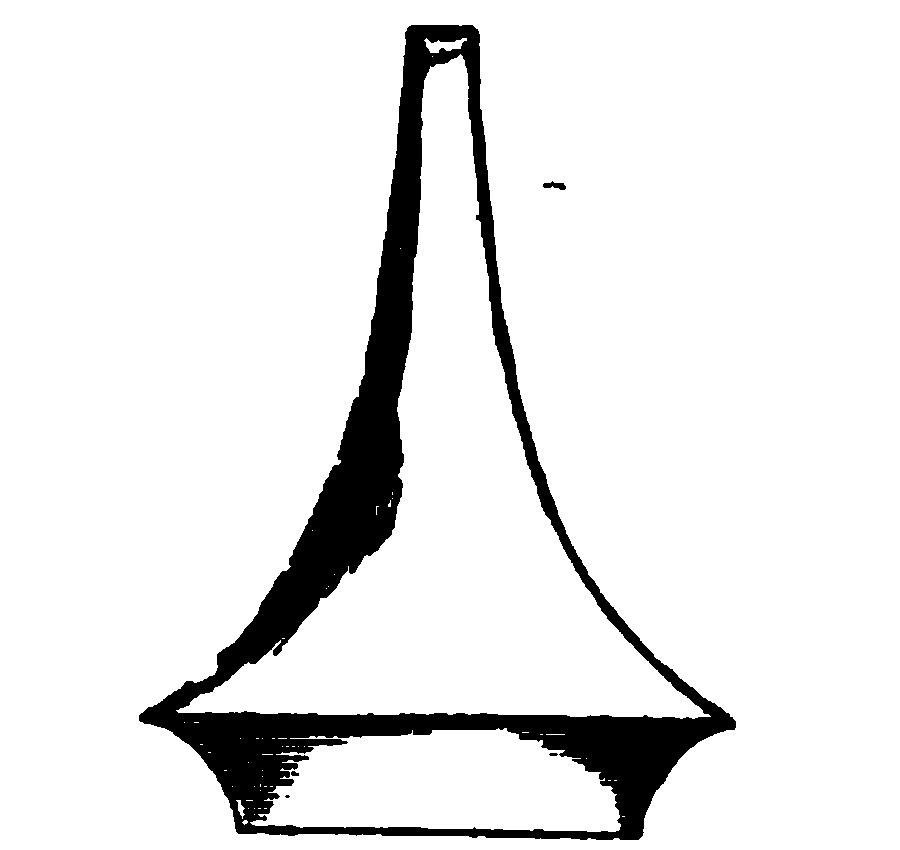
\includegraphics[width=0.82\linewidth]{assets/ch07_figures/F1_EMBED_DETERMINISTIC_GRAY8.png}\\[-.2em]
{\footnotesize\bfseries 图1.\({}^{\rm a}\)--伪球面。}
\end{minipage}
\end{center}

\emph{情形 II：椭圆型。} 为得到实曲面，必须假设
\[
 \frac{\lambda}{R}<1
\]
令 \(\lambda=R\sen\alpha\)，则 \(\cosh\dfrac{u}{R}\) 的最大值为 \(\dfrac1{\sen\alpha}\)，所以平行圆半径 \(r\) 在
\[
 r=0
 \qquad\hbox{e}\qquad
 r=R\cos\alpha.
\]
当 \(r=0\) 时，\(\dfrac{dr}{du}=\sen\alpha\)；因此所有子午线都在 \(u=0\) 处以角 \(\alpha\) 与旋转轴相交，这一点是曲面的锥点。

子午曲线上一点的坐标可表示为参数 \(\tau\) 的椭圆函数，其模为 \(k=\cos\alpha\)。事实上，令
\[
 \senh\frac{u}{R}=\frac{k}{k'}\cn(\tau,k)
\]
便有
\[
 r=Rk\cn\tau,
 \qquad
 z=Rk'\int_0^\tau \sn^2\tau\,d\tau
 =R\left\{\frac{H}{K}\tau-Z(\tau)\right\},
\]
其中
\[
 Z(\tau)=\frac{\Theta'(\tau)}{\Theta(\tau)}
\]
是 Jacobi 函数，H、K 是椭圆函数理论中的熟知常数。曲线上从 \(\tau=0\) 到 \(\tau=2K\) 的一段绘于图 II)；当 \(\tau\) 增加 \(4K\) 时，曲线周期性重复。相应的旋转面由沿轴平移后全等的无穷多个部分组成；半径 \(r=R\cos\alpha\) 的最大平行圆是曲面的回归线，因为 \(\tau=2mK\)（\(m\) 为整数）处是子午曲线的尖点。

\begin{center}
\begin{minipage}{0.55\linewidth}
\centering
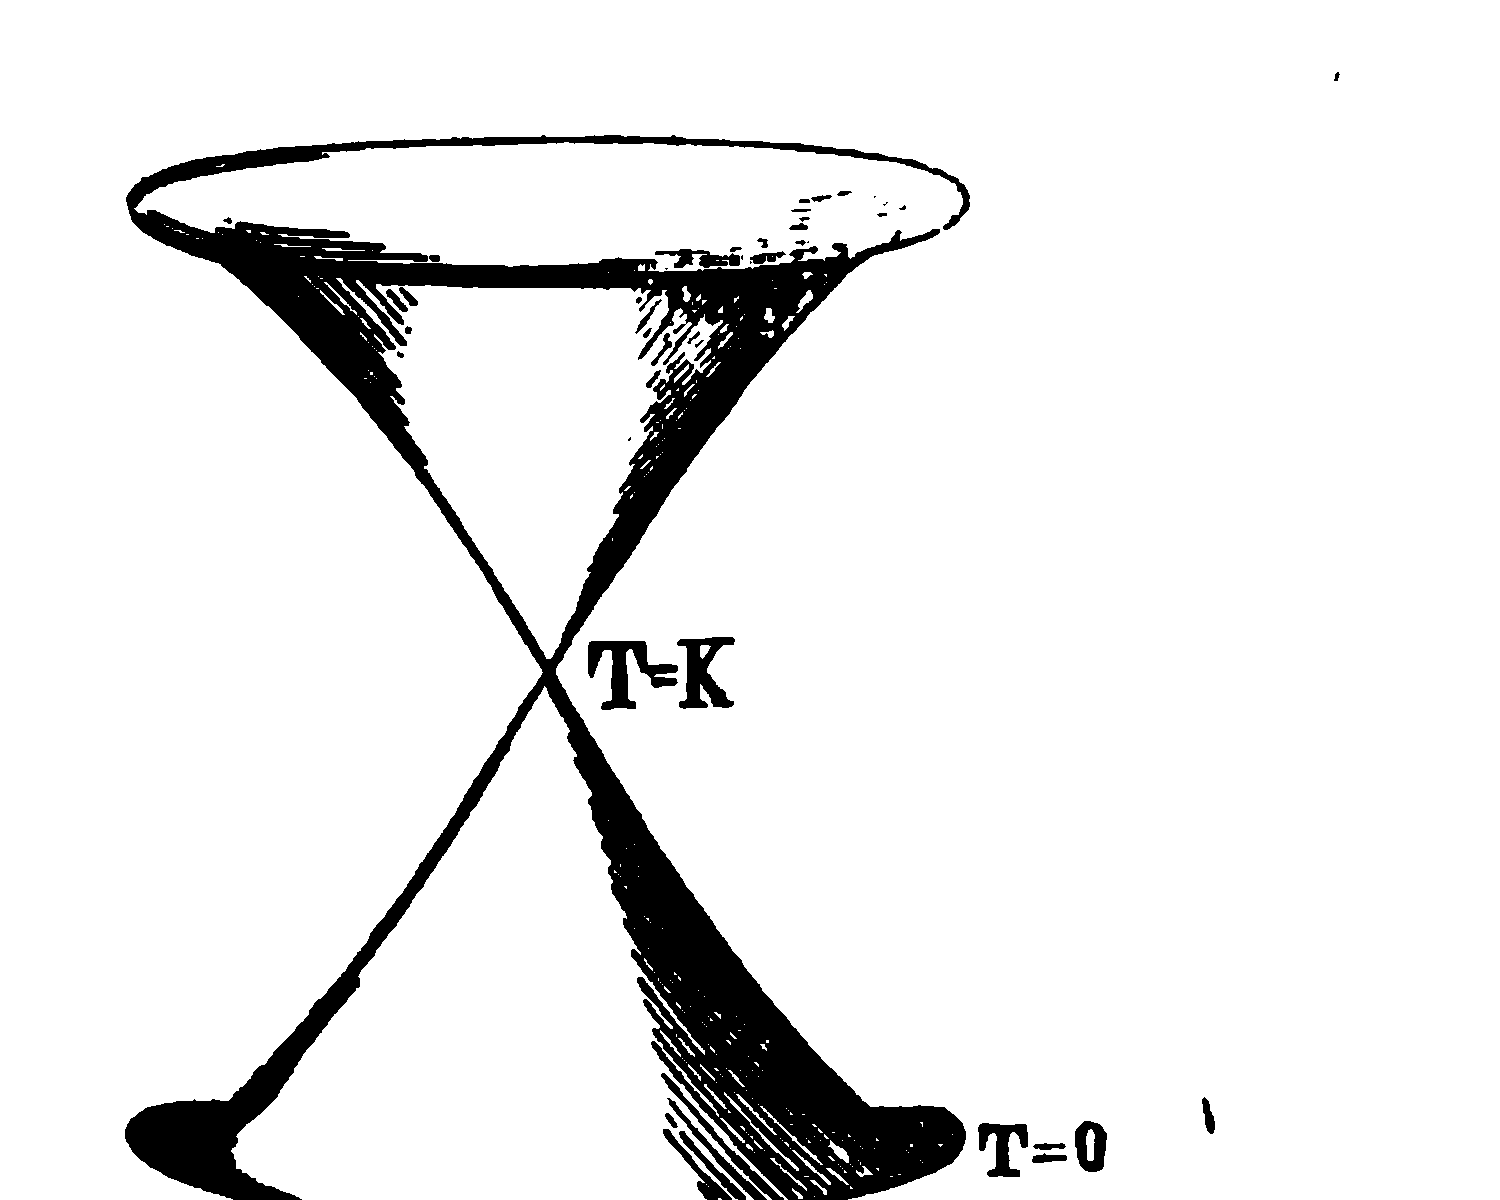
\includegraphics[width=0.96\linewidth]{assets/ch07_figures/F2_EMBED_DETERMINISTIC_GRAY8.png}\\[-.2em]
{\footnotesize\bfseries 图2.\({}^{\rm a}\)--椭圆型伪球旋转面。}
\end{minipage}
\end{center}

\emph{情形 III：双曲型。} 此时
\[
 r=\lambda\cosh\frac{u}{R},
 \qquad
 \frac{dr}{du}=\frac{\lambda}{R}\senh\frac{u}{R};
\]
曲线实部中 \(u\) 的最大值对应于 \(\senh\dfrac{u}{R}=\dfrac{R}{\lambda}\)，而平行圆半径在最小值 \(\lambda\) 与最大值 \(\sqrt{R^2+\lambda^2}\) 之间变化。

令
\[
 \frac{R}{\sqrt{R^2+\lambda^2}}=k,
 \qquad
 \cosh\frac{u}{R}=\frac{\dn(\tau,k)}{k},
\]
则曲线上动点的坐标可由参数 \(\tau\) 的椭圆函数表示为
\[
 r=\frac{R}{k}\dn\tau,
 \qquad
 z=\frac{R}{k}\left\{\frac{H}{K}\tau-Z(\tau)\right\}.
\]
从 \(\tau=0\) 到 \(\tau=2K\) 的曲线形状绘于图3.\({}^{\rm a}\)；当 \(\tau\) 增加 \(2K\) 时，曲线周期性重复。对应于 \(\tau=2mK\)（\(m\) 为整数）的最大平行圆是曲面的回归线，而对应于 \(\tau=(2m+1)K\) 的最小平行圆是测地线。

\begin{center}
\begin{minipage}{0.48\linewidth}
\centering
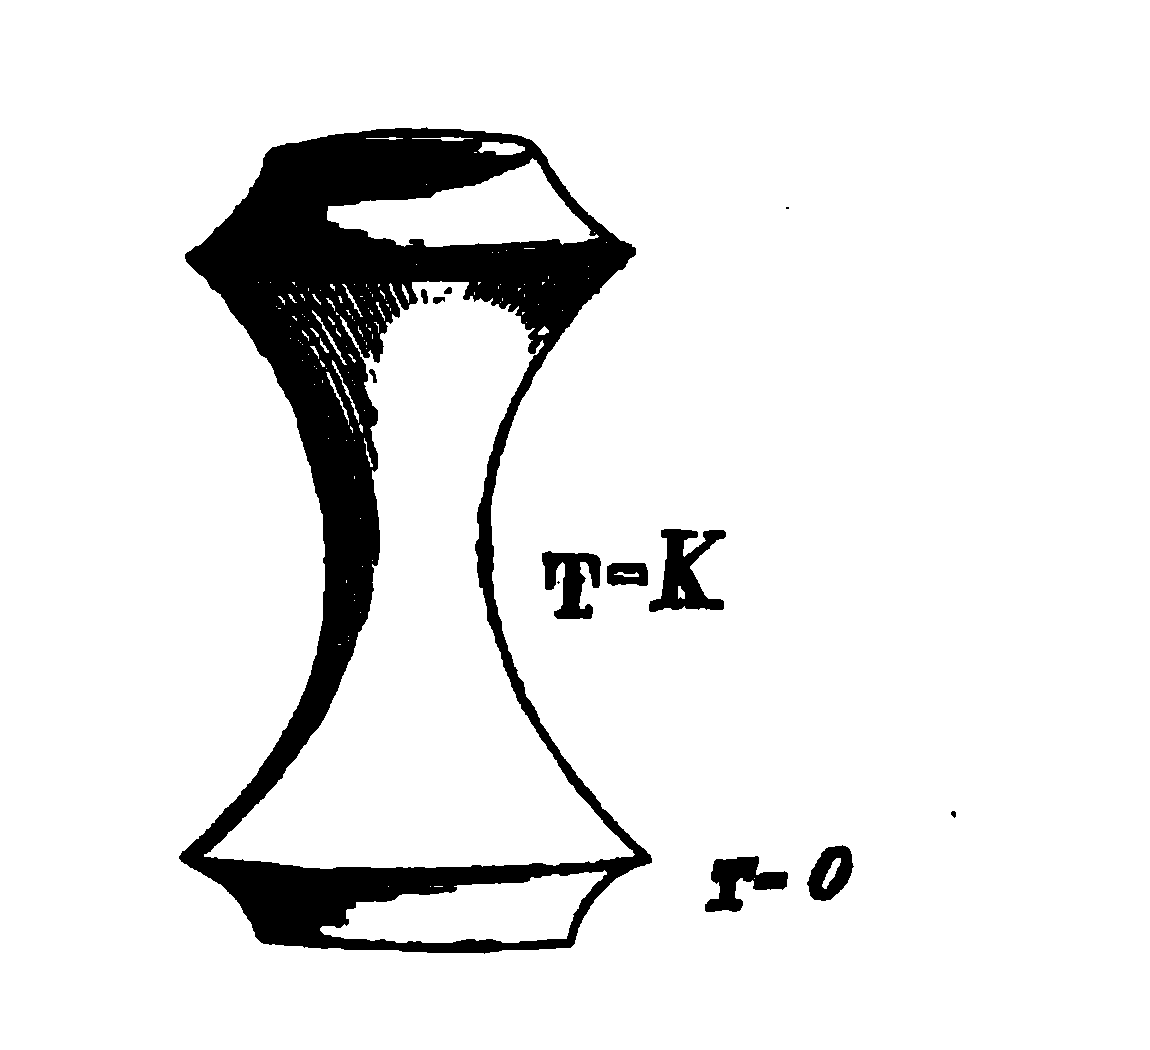
\includegraphics[width=0.85\linewidth]{assets/ch07_figures/F3_EMBED_DETERMINISTIC_GRAY8.png}\\[-.2em]
{\footnotesize\bfseries 图3.\({}^{\rm a}\)--双曲型伪球旋转面。}
\end{minipage}
\end{center}

以上三种伪球旋转面彼此不同；也不可能把其中一种等距适用于另一种不同类型的曲面，同时使平行圆仍铺展到平行圆上。只须注意：抛物型中平行圆的测地曲率恒为 \(\dfrac1R\)，椭圆型中为 \(>\dfrac1R\)，而双曲型中为 \(<\dfrac1R\)，即可判明这一点。不过由一般定理（\S.100），任一半径为 R 的伪球面都能等距适用于 I)、II)、III) 中的每一个曲面。为更仔细说明任一伪球面变形为旋转面的方式，作如下观察：

a) 在伪球面 S 上画一条极限圆，并考察与它正交的测地线。通过弯曲，可使该曲面成为伪球面，而所画测地线变成子午线。

b) 在伪球面 S 上标出一点 P，考察从 P 发出的测地线及其正交的测地圆。按第224页选取参数 \(u,v\)，便有
\[
 ds_1^2=du^2+R^2\senh^2\frac{u}{R}\,dv^2.
\]
与椭圆型旋转面的线元
\[
 ds_1^2=du_1^2+\lambda^2\senh^2\frac{u_1}{R}\,dv_1^2,
\]
比较，得到等距适用公式
\[
 u_1=u,
 \qquad
 \frac{\lambda}{R}v_1=v.
\]
由此可见，当旋转面 II) 上的经度 \(v_1\) 从 0 到 \(2\pi\) 转过一整圈时，角 \(v\) 只遍历从 \(v=0\) 到 \(v=2\pi\sen\alpha<2\pi\) 的区间。因此，S 上 P 附近的一部分就足以完全覆盖曲面 II) 的一叶。此外，S 上位于半径为
\[
 u=\sett\cosh\left(\frac1{\sen\alpha}\right)
\]
的测地圆之外的部分，在曲面 II) 上没有对应点；因而 S 上可变形成曲面 II) 一叶的 P 邻域，由一个测地扇形界定。

c) 对于双曲型曲面 III)，最小平行圆是一条测地线；因此可把任一伪球面 S 等距适用于 III)，使 S 的任意测地线 \(g\) 铺展到该最小平行圆上。S 上实际铺到 III) 一叶上的部分，是一个带状区域：其两侧由两条与 \(g\) 测地平行且到它等距的曲线界定，这两条曲线变形后成为该叶的最大平行圆（回归线）；沿测地线 \(g\) 的方向，该带又由两条与 \(g\) 正交的测地线界定，它们变形后合并为该叶的一条子午线。带的长度和宽度只取决于拟赋予最小平行圆的半径。

\subsection*{\S. 104.\quad 容许在自身上作 \(\infty^1\) 个等距适用的曲面。}

在 \S.100 证明的常曲率曲面之基本性质，可以表述为：

\emph{任一常曲率曲面的线元都容许一个 \(\infty^3\) 的自身变换族。}

现在问：是否还有别的曲面容许在自身上作连续弯曲？若这种弯曲构成一个双参数族，那么利用变换的两个参数，可以把曲面的每一点移到（某一适当区域内的）任意另一点；由高斯定理，该曲面必有常曲率，而所假定的弯曲就应构成三参数族，而不是双参数族。

显然，任何等距适用于某一旋转面的曲面，都容许在自身上作连续弯曲；这种弯曲对应于该旋转面绕轴的旋转。

重要的是，逆定理也成立：

\emph{凡容许在自身上作连续弯曲的曲面 S，都等距适用于某一旋转面。} 这一点实质上已由 \S.99 的讨论得到，因为那里看出：两个曲面 S、S' 的等距适用公式只有在它们都等距适用于同一旋转面时，才能含有一个任意参数。不过也可由以下几何论证重新证明。若 S 具有常曲率，前几节已经证明该定理；否则，在所假定的连续弯曲中，等曲率线 L
\[
 K=\hbox{常数}
\]
由高斯定理必沿自身滑动。由于这种弯曲依赖于一个连续变化的参数，L 上任一点都能移到 L 上任意另一点；所以 L 具有常测地曲率。此外，与某条 L 测地平行的各条曲线，在上述弯曲中也显然沿自身滑动。由此容易推出所述定理；事实上成立如下性质：

\emph{若曲面 S 具有一个由测地平行且测地曲率为常数的曲线 L 组成的线系，那么 S 等距适用于某一旋转面，而该旋转面的平行圆正是曲线 L 的变形。}

事实上，取曲线 L（\(u=\) 常数）及其正交测地线（\(v=\) 常数）组成的坐标系；线元成为
\[
 ds^2=du^2+G\,dv^2.
\]
按假设有
\[
 -\frac1{\rho_u}=\frac{\partial\log\sqrt G}{\partial u}=\varphi(u),
\]
所以
\[
 \sqrt G=UV,
\]
其中 U 只是 \(u\) 的函数，V 只是 \(v\) 的函数。令
\[
 \int V\,dv=v_1,
\]
便显出线元
\[
 ds^2=du^2+U^2\,dv_1^2
\]
属于一个旋转面。

\subsection*{\S. 105.\quad 彼此等距适用的旋转面。}

现在考察一些等距适用曲面的简单例子。首先研究两个旋转面 S、S\(_1\) 能否彼此等距适用。

首先由高斯定理，S 的平行圆必铺展到 S\(_1\) 的平行圆上，因而子午线也铺展到子午线上。常曲率曲面当然是例外；但若附加一个曲面的平行圆铺到另一个曲面平行圆上的条件，以下论证对它们也成立。

若 S 的线元为
\[
 ds^2=du^2+r^2\,dv^2
\]
而 S\(_1\) 的线元为
\[
 ds_1^2=du_1^2+r_1^2\,dv_1^2,
\]
从两个对应平行圆起算子午线弧长，便可直接令 \(u_1=u\)。为使两个线元相互变换，令 \(v_1=v_1(v)\)，并由条件
\[
 r_1(u)\frac{dv_1}{dv}=r(u).
\]
确定该函数。由此得
\[
 r_1=kr,
 \qquad
 v_1=\frac{v}{k}\quad (k\hbox{ 为任意常数}).
\]
因此，若 \(r=\varphi(u)\) 是 S 的子午曲线方程，则 S\(_1\) 的子午曲线坐标为
\[
 r=k\varphi(u),
 \qquad
 z=\int\sqrt{1-k^2\varphi'^2(u)}\,du.
\]
所以：\emph{每个旋转面都能以一个 \(\infty^1\) 的方式族变形，同时仍保持为旋转面。}

再仔细考察 S\(_1\) 等距适用于 S 的方式。若设 \(k<1\)，公式
\[
 v=kv_1
\]
表明：当经度 \(v_1\) 在 S\(_1\) 上转过一整圈而成为 \(2\pi\) 时，经度 \(v\) 变为
\[
 v=2k\pi<2\pi.
\]
所以把 S\(_1\) 铺到 S 上时，S 不会被完全覆盖；两条子午线之间会留下一个扇形部分，其所在平面的夹角为 \(2\pi(1-k)\)。要把 S\(_1\) 铺展到 S 上，必须先沿一条子午线切开 S\(_1\)，再把它张开并变形，使切口的两条边在 S 上成为两条不同的子午线。注意平行圆的测地曲率和曲面的总曲率在变形中不变，立即可知：在对应点上，S 的子午曲线曲率大于 S\(_1\) 的子午曲线曲率。

情形 \(k>1\) 显然对应于 S 到 S\(_1\) 的逆变形：须从 S 去掉一个扇形，再把被去掉扇形的两条子午线通过变形合成一条，以恢复曲面的连续性。还应注意，S 子午曲线上的一点在 S\(_1\) 的子午曲线上有实对应点，只要 \(k\dfrac{dr}{du}<1\)；当 \(k<1\) 时这总是成立。但当 \(k>1\) 时，对应于 \(\dfrac1k\) 这个 \(\dfrac{dr}{du}\) 值的平行圆在 S 上界定出一个带状区域，这才是 S 中实际能等距适用于 S\(_1\) 的部分。变形后，该带的两个边界平行圆成为 S\(_1\) 的回归平行圆。

作为例子，考察常曲率旋转面的变形。

a) 对半径为\emph{一}的球面，可取
\[
 r=\cos u
\]
变形后的子午曲线坐标为
\[
 r=k\cos u,
 \qquad
 z=\int\sqrt{1-k^2\sen^2 u}\,du.
\]
可把它们表示为参数 \(\tau\) 的椭圆函数。若 \(k<1\)，令 \(\cos u=\cn(\tau,k)\)，则
\[
 r=k\cn\tau,
 \qquad
 z=\left(1-\frac{H}{K}\right)\tau+Z(\tau);
\]
若 \(k>1\)，把 \(k\) 换成 \(\dfrac1k\)，并令
\[
 \cos u=\dn(\tau,k)
\]
则
\[
 r=\frac{\dn\tau}{k},
 \qquad
 z=\left(k-\frac{H}{Kk}\right)\tau+\frac1k Z(\tau).
\]
当 \(k<1\) 时，得到一个纺锤形曲面，其子午线以角 \(\alpha=\arc\sen k\) 在一点与轴相交；该点是曲面的锥点。当 \(k>1\) 时，得到一个由两个最小回归平行圆界定的带状区域。以下三图分别表示这三种情形所对应的曲面；在中间的球面上，标出了能等距适用于图6.\({}^{\rm a}\) 曲面的区域。

\begin{center}
\begin{minipage}[t]{0.29\linewidth}
\centering
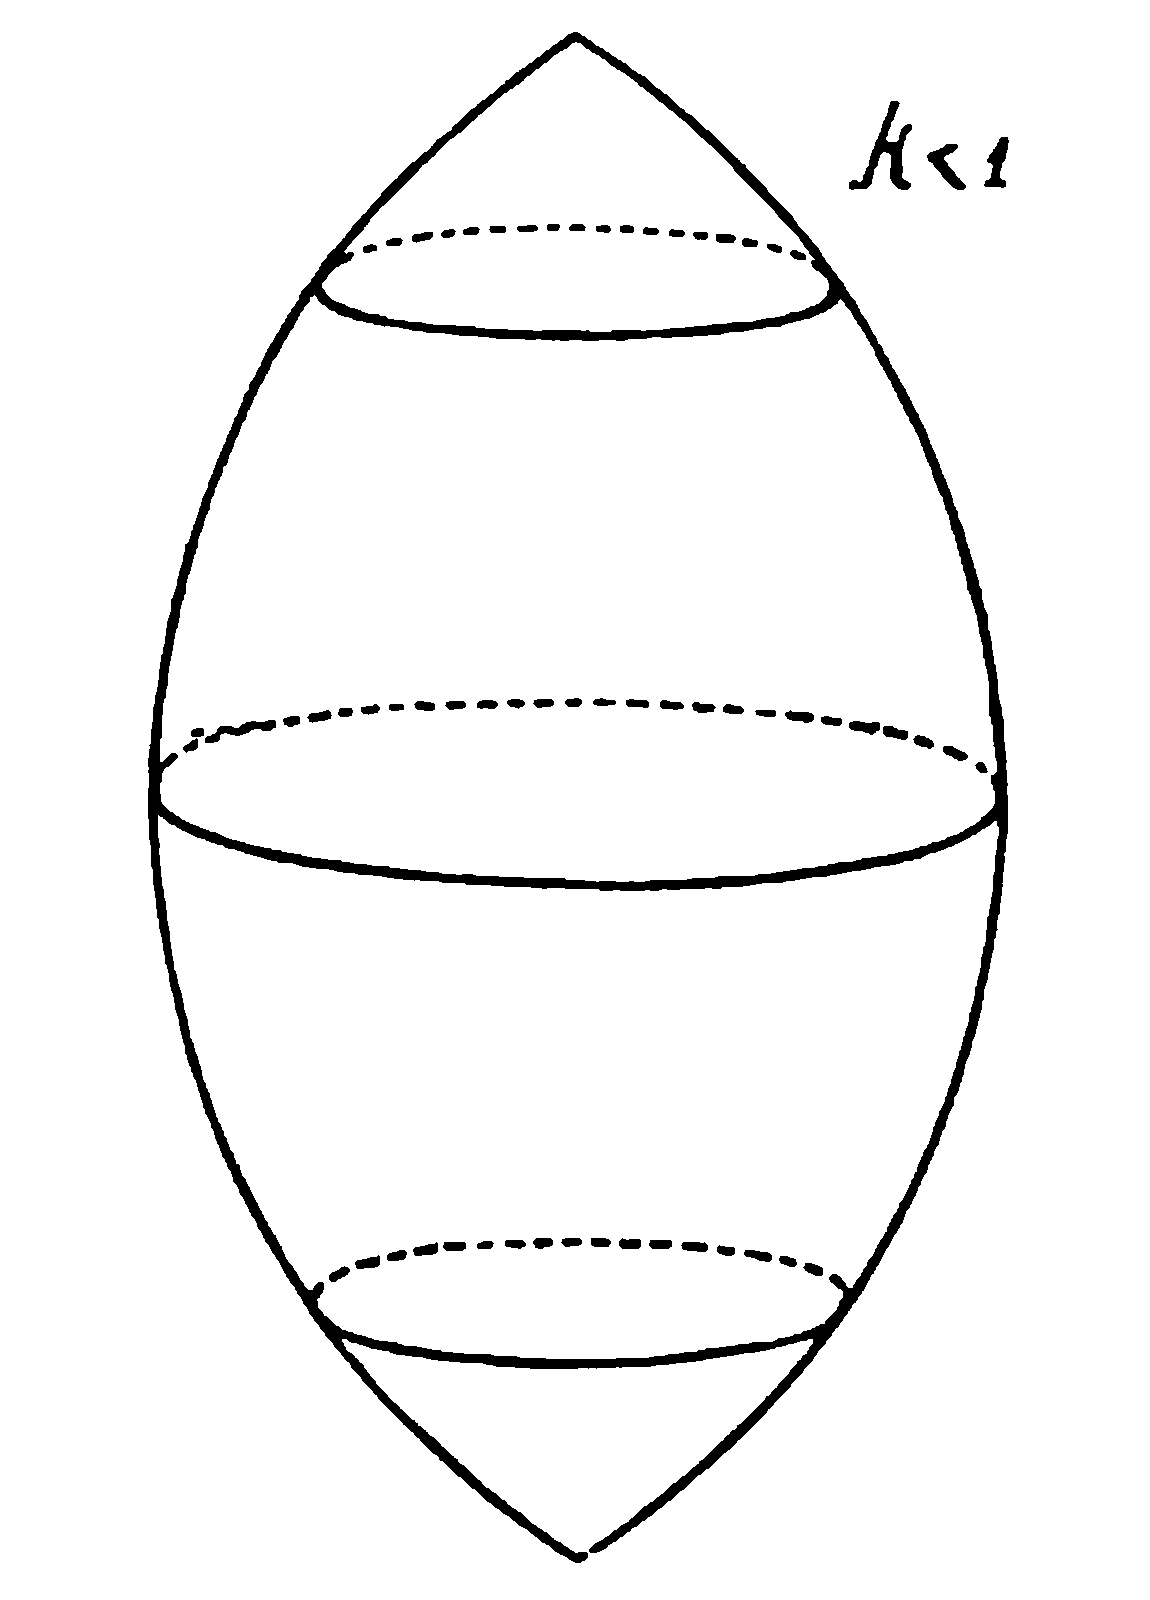
\includegraphics[width=0.92\linewidth]{assets/ch07_figures/F4_EMBED_DETERMINISTIC_GRAY8.png}\\[-.2em]
{\footnotesize\bfseries 图4.\({}^{\rm a}\)}
\end{minipage}\hfill
\begin{minipage}[t]{0.37\linewidth}
\centering
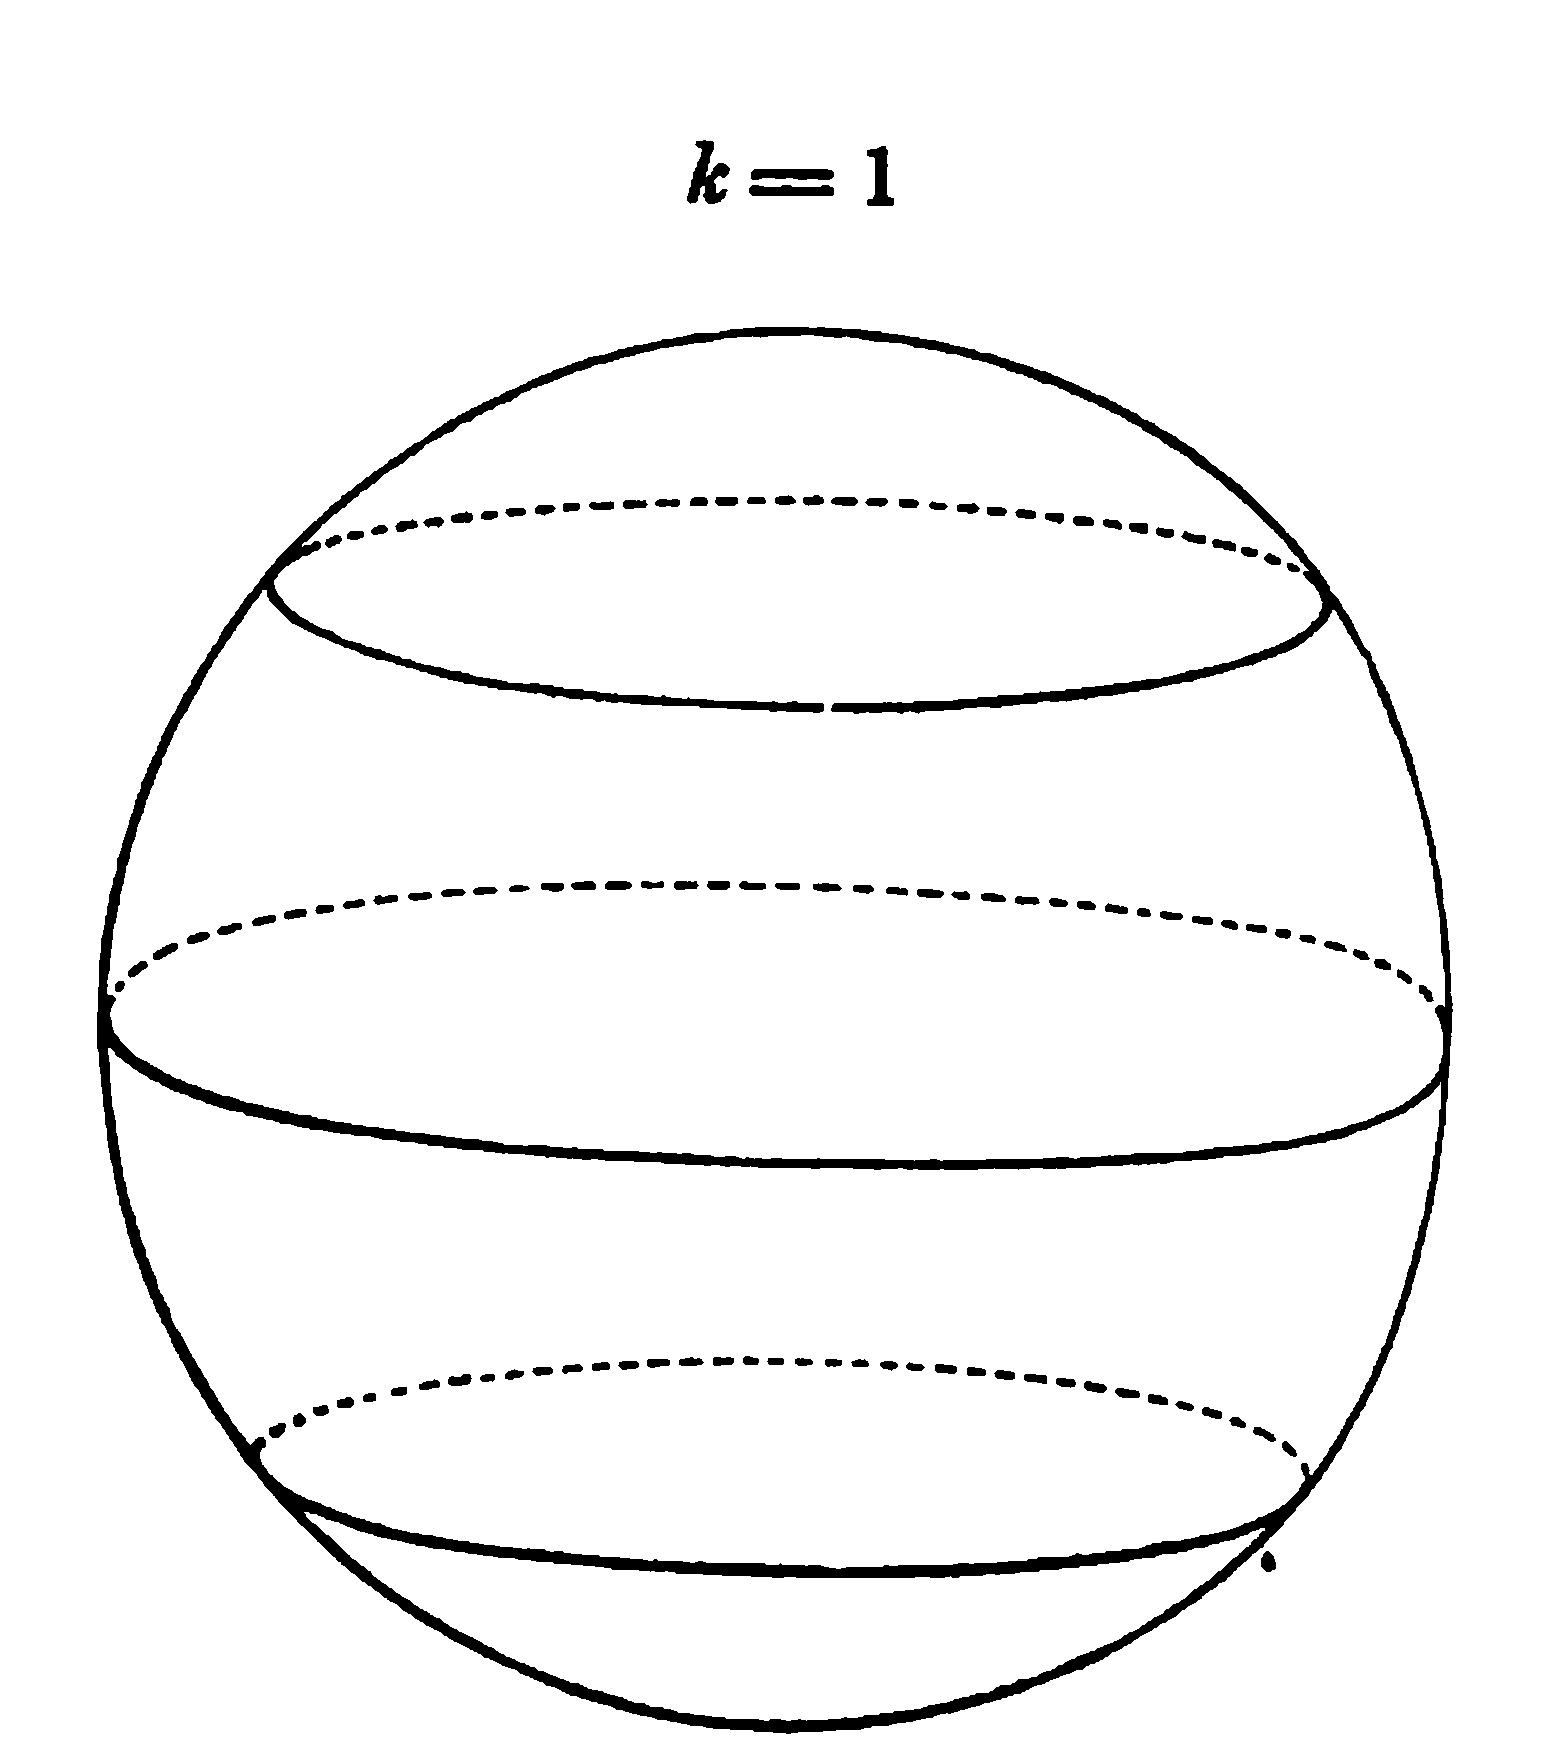
\includegraphics[width=0.98\linewidth]{assets/ch07_figures/F5_EMBED_DETERMINISTIC_GRAY8.png}\\[-.2em]
{\footnotesize\bfseries 图5.\({}^{\rm a}\)--（球面）。}
\end{minipage}

\medskip
\begin{minipage}{0.48\linewidth}
\centering
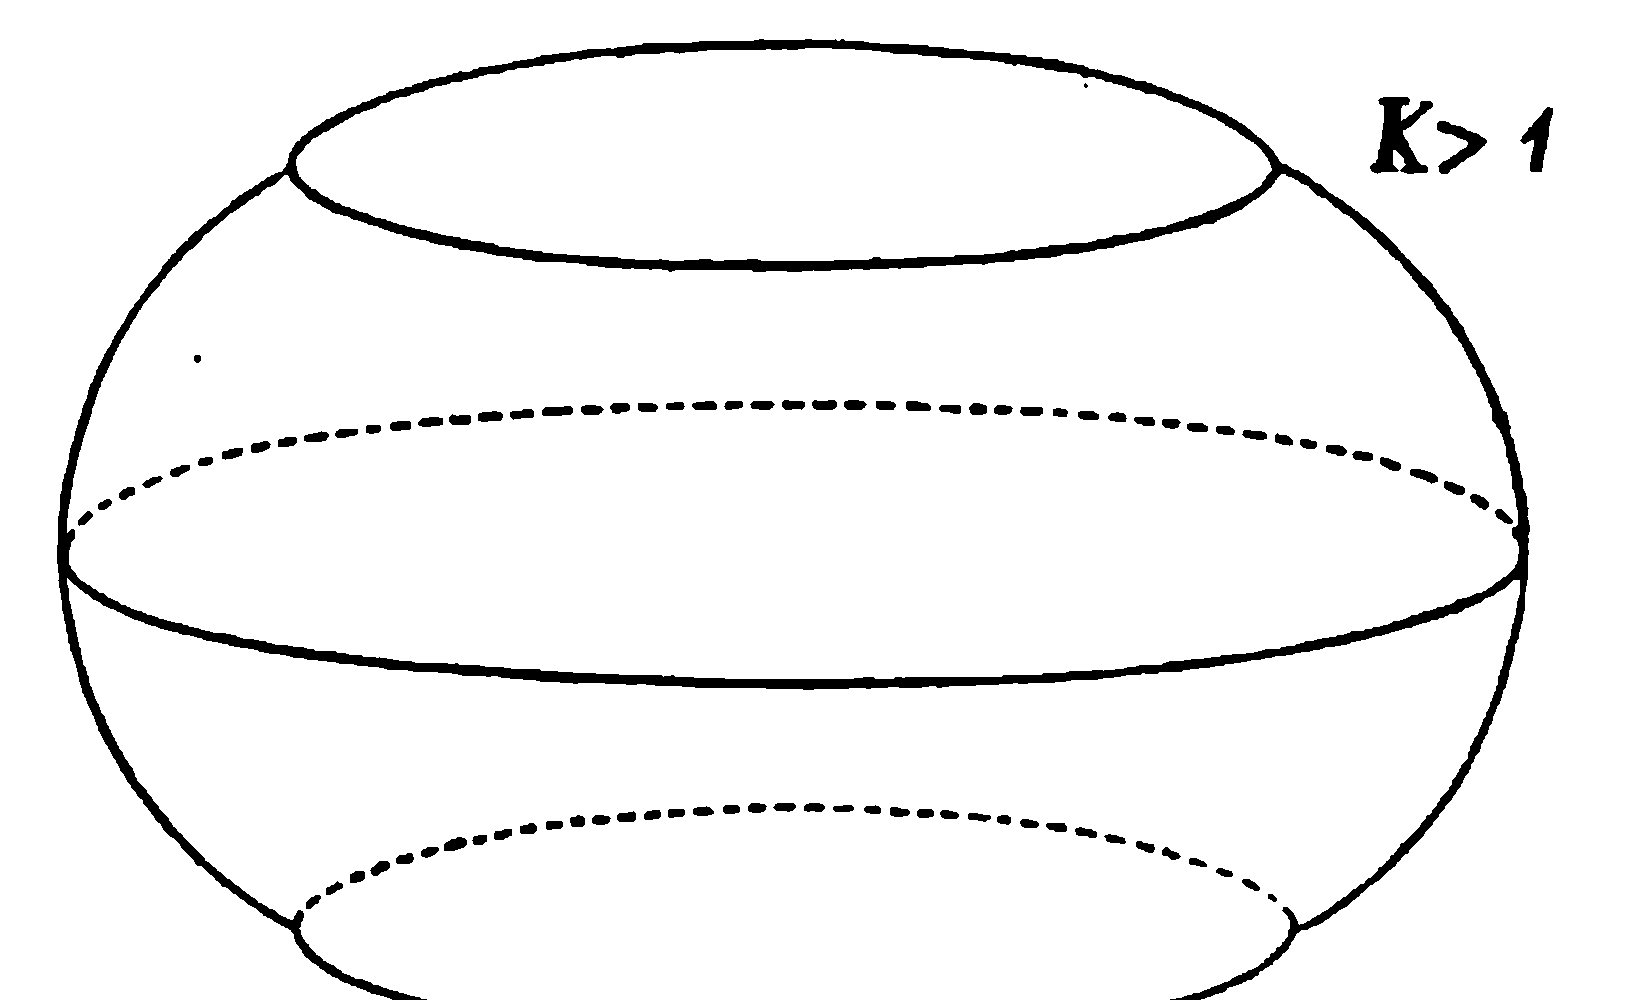
\includegraphics[width=0.98\linewidth]{assets/ch07_figures/F6_EMBED_DETERMINISTIC_GRAY8.png}\\[-.2em]
{\footnotesize\bfseries 图6.}
\end{minipage}
\end{center}

b) 伪球面具有一个特殊性质：它的所有旋转变形都与伪球面本身重合。这由平行圆的测地曲率恒 \(=\dfrac1R\) 立即可见。

在平行圆收缩的情形（\(k<1\)）中，最大平行圆（回归线）变成一个较小的平行圆，因而该平行圆与最大平行圆之间的带状区域未被覆盖。在逆变形中，一个较小的平行圆变成回归平行圆；但要实现这种变形，必须先从伪球面上切去该平行圆与现有回归平行圆之间的区域。

另外两类伪球旋转面的变形仍得到同类型的曲面：椭圆型中改变顶点（锥点）的张角，双曲型中改变最小平行圆的半径。

\subsection*{\S. 106.\quad 螺旋面与 Bour 定理。}

\S.104 的结果可立即应用于一类重要曲面，称为\emph{螺旋面}。这类曲面由一条平面曲线或空间曲线生成：曲线一面绕某轴旋转，一面沿该轴平移，而且两种运动的速度之比为常数。母线的各点分别描出圆螺线，它们以螺旋面的轴为共同轴，并具有同一螺距。生成曲面的螺旋运动使整个曲面沿自身滑动；应用 \S.105 的定理，便得到 Bour 的优美结果：

\emph{每个螺旋面都等距适用于一个旋转面；螺线铺展为平行圆。}

显然，该旋转面被螺旋面覆盖无穷多次，因为每条螺线都绕相应的平行圆无穷多圈。

现在直接证明该定理，同时求出实际的等距适用公式。过轴作一平面，它在螺旋面上截出一条曲线；若使这条截线（\emph{子午剖线}）作生成该曲面的螺旋运动，它便描出整个螺旋面。给定子午剖线和螺旋运动的参数，螺旋面就完全确定。

取螺旋面的轴为 \(z\) 轴，以 \(\rho\) 表示子午剖线上一点到该轴的距离，设
\[
 z=\varphi(\rho)
\]
为子午剖线的方程。再以 \(v\) 表示经过任意时间后子午剖面所转过的角，以 \(m\) 表示平移速度与旋转速度之比。螺旋面上动点的坐标 \(x,y,z\) 作为 \(\rho,v\) 的函数为
\[
 x=\rho\cos v,
 \qquad y=\rho\sen v,
 \qquad z=\varphi(\rho)+mv,
\]
从中
\[
 ds^2=\{1+\varphi'^2(\rho)\}\,d\rho^2+2m\varphi'(\rho)\,d\rho\,dv+(\rho^2+m^2)\,dv^2.
\]
变换坐标线 \(v\)，令
\[
 v=kv_1-m\int\frac{\varphi'(\rho)\,d\rho}{\rho^2+m^2},
\]
其中 \(k\) 为任意常数；于是
\[
 ds^2=\left\{1+\frac{\rho^2\varphi'^2(\rho)}{\rho^2+m^2}\right\}d\rho^2+k^2(\rho^2+m^2)\,dv_1^2.
\]
把这个线元与旋转面的线元
\[
 ds_1^2=\{1+\psi'^2(r)\}\,dr^2+r^2dv_1^2
\]
相比较；其中
\[
 z=\psi(r)
\]
是子午曲线方程。若令 \(r,\psi(r),\rho,\varphi(\rho)\) 满足关系
\begin{equation}\tag{8}
\left\{
\begin{aligned}
 r^2&=k^2(\rho^2+m^2),\\
 \{1+\psi'^2(r)\}\left(\frac{dr}{d\rho}\right)^2
 &=1+\frac{\rho^2\varphi'^2(\rho)}{\rho^2+m^2}.
\end{aligned}
\right.
\end{equation}
便能使两个线元相同。这些公式再次证明 Bour 定理；而且还表明：任取一个螺旋面或一个旋转面，都可用求积找出与之等距适用的旋转面或螺旋面。第一种情形中消去 \(\rho\)，便得到 \(\psi'(r)\)；第二种情形中消去 \(r\)，便得到 \(\varphi'(\rho)\)。

\subsection*{\S. 107.\quad 极小直纹螺旋面与单叶双曲面。}

把公式 (8) 应用于两个简单例子。

1. 子午剖线是一条垂直于轴的直线；所生成的螺旋面就是第一章 \S.24 已考察的\emph{极小直纹螺旋面}。此时 (8) 中 \(\varphi'(\rho)=0\)，所以
\[
 1+\psi'^2(r)=\left(\frac{d\rho}{dr}\right)^2=\frac{r^2}{k^2(r^2-m^2k^2)}
\]
取任意常数 \(k=1\)，得到
\[
 z=\psi(r)=m\int\frac{dr}{\sqrt{r^2-m^2}}
\]
作此求积便有
\[
 r=m\cosh\frac{z}{m}.
\]
所以子午曲线是一条普通悬链线，其准线为旋转轴。

相应的旋转面称为\emph{悬链面}。螺旋面的直母线铺展到子午线上，而轴 \(\rho=0\) 变成悬链面的腰圆 \(r=m\)。

2. 子午剖线是一条与轴成角 \(\alpha\) 的直线；其方程为
\[
 z=\rho\cot\alpha
\]
把
\[
 \varphi'(\rho)=\cot\alpha,
\]
代入 (8)，得到
\[
 1+\psi'^2(r)=\left\{1+\frac{(r^2-k^2m^2)\cot^2\alpha}{r^2}\right\}
 \frac{r^2}{k^2(r^2-k^2m^2)}
\]
再令
\[
 k=\cot\alpha,
\]
便有
\[
 \psi'(r)=\frac{\tg\alpha\,r}{\sqrt{r^2-m^2\cot^2\alpha}}.
\]
所以旋转面的子午曲线方程为
\[
 z=\tg\alpha\sqrt{r^2-m^2\cot^2\alpha},
\]
即
\[
 \frac{r^2}{m^2\cot^2\alpha}-\frac{z^2}{m^2}=1.
\]
因此，该旋转面是单叶旋转双曲面。容易看出，螺旋面的轴 \(\rho=0\) 铺展到双曲面的腰圆上，而螺旋面的直母线铺展到双曲面一个直母线系的母线上。

\subsection*{\S. 108.\quad 第二个等距适用问题。}

现在转向等距适用理论的第二个、也是更重要的问题：\emph{求出所有等距适用于给定曲面的曲面}，或者说：\emph{求出具有给定线元的所有曲面}。

这个困难问题只有在少数特殊情形中知道如何完全解决；后文将考察这些情形。不过，偏微分方程的一般定理使我们能建立一些关于该问题的极重要的一般结果。现在就在本书篇幅所容许的范围内讨论这些结果\srcfn{1}{读者可在 Darboux《讲义》第三卷第263页及以下找到这个问题的完整论述。}。

处理这一问题的第一种方法自然来自曲面论的基本公式（第四章）。给定第一基本形式
\[
 E\,du^2+2F\,du\,dv+G\,dv^2,
\]
每一个具有此线元的曲面都对应一个第二基本形式
\[
 D\,du^2+2D'\,du\,dv+D''\,dv^2,
\]
函数 \(D,D',D''\) 必须满足 \S.56（第119页）的方程 (III)、(IV)，即高斯方程与两个 Codazzi 方程。反过来，若 \(D,D',D''\) 是满足这三个方程的 \(u,v\) 的函数，就存在一个具有给定线元的对应曲面；实际求出该曲面还须解一个 Riccati 方程。

例如，若取旋转面的线元
\[
 ds^2=du^2+r^2dv^2,
\]
就可令 \(D,D',D''\) 只为 \(u\) 的函数来满足上述基本方程。这样得到的等距适用于旋转面的曲面，恰是 \S.106 的螺旋面\srcfn{1}{为证明这一点，只须注意此时第一、第二基本形式都容许连续的自身变换
\[
 u'=u,\qquad v'=v+\hbox{常数}
\]
因此曲面容许在自身上的连续运动，故为螺旋面。}。

\subsection*{\S. 109.\quad 第二个问题的偏微分方程。}

比前一种方法更重要的是下面的方法；它以 \S.69 所得结果，确切地说以第146页方程 (B) 为基础。

对于任一曲面
\[
 x=x(u,v),\qquad y=y(u,v),\qquad z=z(u,v)
\]
若其给定线元为
\begin{equation}\tag{9}
 dx^2+dy^2+dz^2=E\,du^2+2F\,du\,dv+G\,dv^2
\end{equation}
上述方程表明，三个未知函数 \(x,y,z\) 中的每一个都满足二阶偏微分方程
\begin{equation}\tag{10}
 \Delta_{22}x=(1-\Delta_1x)K,
\end{equation}
其系数正由 \(E,F,G\) 及其一阶、二阶导数构成\srcfn{2}{采用 Monge 记号，以 \(p,q;r,s,t\) 表示未知函数的一阶、二阶导数，方程写成
\[
\begin{aligned}
&\left(r-\chr{1}{1}{1}p-\chr{1}{1}{2}q\right)
 \left(t-\chr{2}{2}{1}p-\chr{2}{2}{2}q\right)
-\left(s-\chr{1}{2}{1}p-\chr{1}{2}{2}q\right)^2 \\
&\hspace{3em}=K\left\{EG-F^2-\left[E q^2-2Fpq+G p^2\right]\right\}
\end{aligned}
\]
它关于 \(rt-s^2\) 及 \(r,s,t\) 具有 Ampère 线性形式。}。

现在应随 Darboux 指出，方程 (10) 具有如下意义：
\begin{center}
\emph{若 \(x(u,v)\) 是它的一个解，则二次形式}
\end{center}
\[
\begin{aligned}
&E\,du^2+2F\,du\,dv+G\,dv^2-dx^2 \\
&=\left\{E-\left(\frac{\partial x}{\partial u}\right)^2\right\}du^2
+2\left\{F-\frac{\partial x}{\partial u}\frac{\partial x}{\partial v}\right\}du\,dv
+\left\{G-\left(\frac{\partial x}{\partial v}\right)^2\right\}dv^2
\end{aligned}
\]
\begin{center}
\emph{具有零曲率。}\end{center}
为以最简方式证明，令
\[
 x=u,
 \qquad F=0,
\]
由方程的不变性，这显然是允许的。于是 (10) 变为
\[
 \chr{1}{1}{1}\chr{2}{2}{1}-\chr{1}{2}{1}^2=G(E-1)K
\]
代入 Christoffel 符号在此时的值
\[
 \chr{1}{1}{1}=\frac1{2E}\frac{\partial E}{\partial u},\qquad
 \chr{1}{2}{1}=\frac1{2E}\frac{\partial E}{\partial v},\qquad
 \chr{2}{2}{1}=-\frac1{2E}\frac{\partial G}{\partial u},
\]
得到
\[
 \frac{\partial E}{\partial u}\frac{\partial G}{\partial u}
 +\left(\frac{\partial E}{\partial v}\right)^2
 +4E^2G(E-1)K=0.
\]
现在在正交坐标中我们有（\S.43，第93页）：
\begin{equation}\tag{11}
\begin{aligned}
4E^2G^2K={}&E\left[\frac{\partial E}{\partial v}\frac{\partial G}{\partial v}+
\left(\frac{\partial G}{\partial u}\right)^2\right]
+G\left[\frac{\partial E}{\partial u}\frac{\partial G}{\partial u}+
\left(\frac{\partial E}{\partial v}\right)^2\right]\\
&-2EG\left[\frac{\partial^2E}{\partial v^2}+\frac{\partial^2G}{\partial u^2}\right]
\end{aligned}
\end{equation}
前一方程乘以 \(G\)，可写成
\[
\begin{aligned}
&G\left[\frac{\partial E}{\partial u}\frac{\partial G}{\partial u}+
\left(\frac{\partial E}{\partial v}\right)^2\right]
+E(E-1)\left[\frac{\partial E}{\partial v}\frac{\partial G}{\partial v}+
\left(\frac{\partial G}{\partial u}\right)^2\right] \\
&\quad+G(E-1)\left[\frac{\partial E}{\partial u}\frac{\partial G}{\partial u}+
\left(\frac{\partial E}{\partial v}\right)^2\right]
-2EG(E-1)\left(\frac{\partial^2E}{\partial v^2}+\frac{\partial^2G}{\partial u^2}\right)=0.
\end{aligned}
\]
消去相互抵消的项并除以 \(E\)，得到等价方程
\[
\begin{aligned}
&(E-1)\left[\frac{\partial E}{\partial v}\frac{\partial G}{\partial v}+
\left(\frac{\partial G}{\partial u}\right)^2\right]
+G\left[\frac{\partial G}{\partial u}\frac{\partial E}{\partial u}+
\left(\frac{\partial E}{\partial v}\right)^2\right]\\
&\qquad -2(E-1)G\left[\frac{\partial^2E}{\partial v^2}+\frac{\partial^2G}{\partial u^2}\right]=0,
\end{aligned}
\]
由 (11) 可知，它恰好表示形式
\[
 (E-1)du^2+Gdv^2
\]
具有零曲率。

在此基础上，设已知方程 (10) 的一个解 \(x(u,v)\)，考察是否存在具有给定线元的对应实曲面。微分形式
\begin{equation}\tag{12}
 E\,du^2+2F\,du\,dv+G\,dv^2-dx^2
\end{equation}
此时具有零曲率。要存在另外两个满足 (9) 的实函数 \(y(u,v),z(u,v)\)，充分必要条件是 (12) 为正定形式，即
\[
\left[E-\left(\frac{\partial x}{\partial u}\right)^2\right]
\left[G-\left(\frac{\partial x}{\partial v}\right)^2\right]
-\left[F-\frac{\partial x}{\partial u}\frac{\partial x}{\partial v}\right]^2>0,
\]
即
\[
 \Delta_1x<1.
\]
若此条件满足，则可用求积求出 \(y,z\)（\S\S.37、93）；显然，\(y,z\) 只差一个坐标变换而确定。

所以：\emph{方程 (10) 的每一个实解 \(x(u,v)\)，若还满足不等式 \(\Delta_1x<1\)，都对应一个且仅一个具有给定线元的实曲面。已知该解后，对应曲面可由求积得到。}

\subsection*{\S. 110.\quad 含有一条刚性曲线时曲面的不可变形性。}

现在考察如下问题：\emph{给定曲面 S 及画在其上的曲线 \(\Gamma\)，能否弯曲该曲面而不使这条曲线变形？}

假设可以，并以 \(S_1\) 表示 S 在弯曲后保持 \(\Gamma\) 刚性不变的一种形状。可设 \(S_1\) 与初始形状充分接近，使 \(S_1\)、S 沿 \(\Gamma\) 的法线任意接近。又因 \(\Gamma\) 在 \(S_1\) 与 S 上具有同一测地曲率，并由测地曲率与绝对曲率的关系（\S.84），立即得出：沿 \(\Gamma\)，\(S_1\) 与 S 的法线重合。

为简单起见，在 S（以及 \(S_1\)）上取正交坐标系 \((u,v)\)，令
\[
 v=0
\]
为曲线 \(\Gamma\) 的方程。以附加下标 1 表示与 \(S_1\) 有关的量，显然有
\[
\left.
\begin{gathered}
 x_1=x,
 \quad y_1=y,
 \quad z_1=z,\\
 \frac{\partial x_1}{\partial u}=\frac{\partial x}{\partial u},\quad
 \frac{\partial y_1}{\partial u}=\frac{\partial y}{\partial u},\quad
 \frac{\partial z_1}{\partial u}=\frac{\partial z}{\partial u},\\
 \frac{\partial x_1}{\partial v}=\frac{\partial x}{\partial v},\quad
 \frac{\partial y_1}{\partial v}=\frac{\partial y}{\partial v},\quad
 \frac{\partial z_1}{\partial v}=\frac{\partial z}{\partial v},\\
 X_1=X,
 \quad Y_1=Y,
 \quad Z_1=Z
\end{gathered}
\right\}\quad \hbox{当 }v=0.
\]
例如考察 \(x_1,x\)：它们是同一个二阶偏微分方程 (10) 的解，并且在 \(v=0\) 上函数值及一阶导数值都相同。若能证明\emph{\(x_1\) 的三个二阶导数也分别等于 \(x\) 的对应二阶导数（在 \(v=0\) 上）}，那么由偏微分方程解的一般定理\srcfn{1}{例如参见 \textsc{Goursat}，\emph{Leçons sur l'intégration des équations aux dérivées partielles du premier ordre}，第22页。}，即可断定 \(x_1,x\) 对一切 \(u,v\) 都相同。对 \(y_1,y;z_1,z\) 重复同一论证，便得到 \(S_1,S\) 重合。由初始条件
\[
 \frac{\partial x_1}{\partial u}=\frac{\partial x}{\partial u},
 \qquad
 \frac{\partial x_1}{\partial v}=\frac{\partial x}{\partial v},
 \quad \hbox{当 }v=0
\]
首先推出
\[
 \frac{\partial^2x_1}{\partial u^2}=\frac{\partial^2x}{\partial u^2},
 \qquad
 \frac{\partial^2x_1}{\partial u\partial v}=\frac{\partial^2x}{\partial u\partial v},
 \quad \hbox{当 }v=0.
\]
于是曲面论的基本公式 (I)（\S.55，第116页）给出
\[
 D_1=D,
 \qquad D'_1=D',
 \quad \hbox{当 }v=0.
\]
等式
\[
 DD''-D'^2=D_1D''_1-D_1'^2,
\]
在 \(v=0\) 上给出
\[
 DD''=DD''_1,
 \quad \hbox{当 }v=0.
\]
因此
\[
 (D''_1)_{v=0}=(D'')_{v=0},
\]
\emph{除非} \((D)_{v=0}=0\)。排除这一情形，由上述 \S.55 公式 (I) 的第三式，正好得到所要证明的
\[
 \frac{\partial^2x_1}{\partial v^2}=\frac{\partial^2x}{\partial v^2},
 \quad \hbox{当 }v=0,
\]
因而 \(S_1,S\) 重合。

在被排除的情形 \((D)_{v=0}=0\) 中，曲线 \(v=0\) 是 S 的渐近线。因此可陈述定理：\emph{若柔性曲面 S 上的一条曲线 \(\Gamma\) 保持刚性，则曲面不能变形；唯一可能的例外是 \(\Gamma\) 为 S 的一条渐近线。}

若 \(\Gamma\) 是渐近线，偏微分方程的进一步性质（这里只能略加指出）表明确实可以在不使该曲线变形的情况下变形曲面。这是渐近线的一个特殊性质，因此渐近线也称为\emph{折线}。它区别于曲面上其他一切曲线，根本原因是：任一曲面 S 的渐近线，正是决定 S 变形的偏微分方程 (10) 的\emph{特征线}\srcfn{1}{把 (10) 写成上一节注中的形式
\[
 \Phi(r,s,t)=0
\]
则特征线的微分方程
\[
 \frac{\partial\Phi}{\partial t}\,du^2-\frac{\partial\Phi}{\partial s}\,du\,dv+\frac{\partial\Phi}{\partial r}\,dv^2=0,
\]
由 \S.55 的公式 (I)，恰变为渐近线的微分方程
\[
 D\,du^2+2D'\,du\,dv+D''\,dv^2=0
\]
（参见\textsc{Darboux}，t.III，第 252 页）。}。

\subsection*{\S. 111.\quad 指定一条曲线变形后形状的曲面变形。}

刚才证明的定理自然引出如下问题：\emph{能否使曲面 \(S'\) 变形，使其上一条指定曲线 C 取得预先给定的形状 \(\Gamma\)？}

首先注意：若所求变形存在，则 \(\Gamma\) 在每一点的绝对曲率必须大于或等于 C 在对应点的测地曲率。设此条件满足；暂且还排除 \(\Gamma\) 的绝对曲率与测地曲率相等的情形，因为那时 \(\Gamma\) 将是变形后曲面上的渐近线。

假设所求变形存在，以 S 表示变形后的曲面。在 S 上像上一节那样取正交坐标系 \((u,v)\)，使曲线 \(\Gamma\) 为 \(v=0\)。为明确起见，再规定参数 \(u\) 是从 \(\Gamma\) 上一固定点起算的弧长，于是
\[
 E=1,
 \quad \hbox{当 }v=0.
\]
以 \(\sigma\) 表示如下有向角：在 \(\Gamma\) 的法平面内，把 S 的正法线方向沿正向转到 \(\Gamma\) 的主法线方向所需转过的角。对曲线 \(\Gamma\) 仍采用曲线论（第一章）的通常记号，则在 \(v=0\) 上有
\begin{equation}\tag{13}
\left\{
\begin{aligned}
\alpha&=\frac{\partial x}{\partial u},
&\beta&=\frac{\partial y}{\partial u},
&\gamma&=\frac{\partial z}{\partial u},\\
\xi&=\cos\sigma\,X-\sen\sigma\,\frac1{\sqrt G}\frac{\partial x}{\partial v},
&\eta&=\cos\sigma\,Y-\sen\sigma\,\frac1{\sqrt G}\frac{\partial y}{\partial v},\\
\zeta&=\cos\sigma\,Z-\sen\sigma\,\frac1{\sqrt G}\frac{\partial z}{\partial v},\\
\lambda&=-\cos\sigma\,\frac1{\sqrt G}\frac{\partial x}{\partial v}-\sen\sigma\,X,
&\mu&=-\cos\sigma\,\frac1{\sqrt G}\frac{\partial y}{\partial v}-\sen\sigma\,Y,\\
\nu&=-\cos\sigma\,\frac1{\sqrt G}\frac{\partial z}{\partial v}-\sen\sigma\,Z.
\end{aligned}
\right.
\end{equation}
又有
\[
 \frac{\partial^2x}{\partial u^2}=\chr{1}{1}{1}\frac{\partial x}{\partial u}+
 \chr{1}{1}{2}\frac{\partial x}{\partial v}+DX=\frac{\xi}{\rho}
\]
以及关于 \(y,z\) 的类似公式；并且由于
\begin{equation}\tag{14}
 \chr{1}{1}{1}_{v=0}=\left(\frac1{2E}\frac{\partial E}{\partial u}\right)_{v=0}=0,
 \qquad
 \chr{1}{1}{2}_{v=0}=-\frac1{2G}\frac{\partial E}{\partial v}=\left(\frac1{\rho_v}\right)_{v=0}-\frac1{\sqrt G},
\end{equation}
与 (13) 比较得到
\begin{equation}\tag{15}
 D=\frac{\cos\sigma}{\rho},
 \qquad
 \frac1{\rho_v}=-\frac{\sen\sigma}{\rho}.
\end{equation}
第二式中，绝对曲率 \(\dfrac1\rho\) 与测地曲率 \(\dfrac1{\rho_v}\) 属于 \(\Gamma\) 且都已知，因而给出未知角 \(\sigma\) 的两个互补值。

取 \(\sigma\) 的这两个值之一；每个值事实上都导向一个相应曲面 S\srcfn{1}{因而本问题有两个不同解，这并不与 \S.110 的定理矛盾。如此得到的两个曲面 S 的确彼此等距适用；在一个曲面连续变形为另一个曲面的过程中，曲线 \(\Gamma\) 最终恢复初始形状，但在中间状态会改变形状。}。由 (13)，在 \(v=0\) 上，\(\dfrac{\partial x}{\partial v},\dfrac{\partial y}{\partial v},\dfrac{\partial z}{\partial v}\) 的初值为
\begin{equation}\tag{16}
\left\{
\begin{aligned}
\frac{\partial x}{\partial v}&=-\sqrt G(\xi\sen\sigma+\lambda\cos\sigma),\\
\frac{\partial y}{\partial v}&=-\sqrt G(\eta\sen\sigma+\mu\cos\sigma),\\
\frac{\partial z}{\partial v}&=-\sqrt G(\zeta\sen\sigma+\nu\cos\sigma).
\end{aligned}
\right.
\end{equation}
还应记下 \(X,Y,Z\) 沿 \(\Gamma\) 的值：
\begin{equation}\tag{11*}
\left\{
\begin{aligned}
X&=\xi\cos\sigma-\lambda\sen\sigma,\\
Y&=\eta\cos\sigma-\mu\sen\sigma,\\
Z&=\zeta\cos\sigma-\nu\sen\sigma.
\end{aligned}
\right.
\end{equation}
由此可知，对方程 (10)
\[
 \Delta_{22}\theta=(1-\Delta_1\theta)K
\]
的这三个解，还知道函数本身以及下列二阶偏导数在 \(v=0\) 上的初值：
\[
 \frac{\partial^2x}{\partial u^2},\quad
 \frac{\partial^2x}{\partial u\partial v},\quad
 \frac{\partial^2y}{\partial u^2},\quad
 \frac{\partial^2y}{\partial u\partial v},\quad
 \frac{\partial^2z}{\partial u^2},\quad
 \frac{\partial^2z}{\partial u\partial v},
\]
它们所满足的偏微分方程 (10)，还会给出\emph{至少其中一个解}的二阶导数
\[
 \frac{\partial^2x}{\partial v^2},\quad
 \frac{\partial^2y}{\partial v^2},\quad
 \frac{\partial^2z}{\partial v^2},
\]
的值；否则，在 \(v=0\) 上，表达式
\[
 \frac{\partial^2x}{\partial u^2}-\chr{1}{1}{1}\frac{\partial x}{\partial u}-\chr{1}{1}{2}\frac{\partial x}{\partial v},
\]
以及关于 \(y,z\) 的两个类似表达式都必须为零。但代入初值并利用 (15) 的第二式，它们分别成为
\[
\frac{\cos\sigma}{\rho}(\xi\cos\sigma-\lambda\sen\sigma),\quad
\frac{\cos\sigma}{\rho}(\eta\cos\sigma-\mu\sen\sigma),\quad
\frac{\cos\sigma}{\rho}(\zeta\cos\sigma-\nu\sen\sigma)
\]
只有在已排除的情形 \(\sigma=\dfrac{\pi}{2}\) 中，它们才会同时为零。因此不失一般性，可设
\[
(\alpha)\qquad \xi\cos\sigma-\lambda\sen\sigma\neq0;
\]
于是，基本方程 (10) 的解 \(x_1(u,v)\) 满足初始条件
\[
(\beta)\qquad x_1=x,
 \quad \frac{\partial x_1}{\partial u}=\alpha,
 \quad \frac{\partial x_1}{\partial v}=-\sqrt G(\xi\sen\sigma+\lambda\cos\sigma)
 \quad \hbox{当 }v=0,
\]
其三个二阶导数的初值也完全确定；因此该解存在且完全确定。另一方面，计算 \(\Delta_1x_1\) 在 \(v=0\) 上的值，得到
\[
 \Delta_1x_1=\left(\frac{\partial x_1}{\partial u}\right)^2+\frac1G\left(\frac{\partial x_1}{\partial v}\right)^2
 =\alpha^2+(\xi\sen\sigma+\lambda\cos\sigma)^2
 =1-(\xi\cos\sigma-\lambda\sen\sigma)^2
\]
所以由条件 (\(\alpha\))，有 \(\Delta_1x_1<1\)（在 \(v=0\) 上）。由于 \(\Delta_1x_1\) 是 \(u,v\) 的连续函数，可知在 \(u,v\) 的某一有限二维区域内仍有 \(\Delta_1x_1<1\)；因而按 \S.109，方程 (10) 的解 \(x_1\) 对应一个具有给定线元、形状完全确定的曲面 \(S_1\)。

\subsection*{\S. 112.\quad 对所得变形曲面的验证。}

经过上一节的讨论，只须验证如此求得的曲面 \(S_1\) 确实满足要求：即在 \(S_1\) 上，曲线 \(C_1\) 的方程为 \(v=0\)，并与给定曲线 \(\Gamma\) 全等。为此应证明，\(C_1\) 与 \(\Gamma\) 在相同弧长 \(u\) 处具有相同的第一曲率和挠率（\S.8）。以下标 1 表示与 \(S_1\) 有关的量。由上一节可知，在 \(v=0\)，即沿 \(C_1\)，\(S_1\) 法线的方向余弦由 (16) 给出；特别地
\[
 X_1=\xi\cos\sigma-\lambda\sen\sigma,
 \quad \hbox{当 }v=0.
\]
在方程
\[
 \frac{\partial^2x_1}{\partial u^2}=\chr{1}{1}{1}\frac{\partial x_1}{\partial u}+
 \chr{1}{1}{2}\frac{\partial x_1}{\partial v}+D_1X_1,
\]
中令 \(v=0\) 并代入相应初值，得到
\[
 \frac{\xi}{\rho}=-\frac1{\rho_v}(\xi\sen\sigma+\lambda\cos\sigma)+D_1(\xi\cos\sigma-\lambda\sen\sigma),
\]
\ednote{原书在这一行的第一个括号中印作 \(\xi\sen\sigma-\lambda\sen\sigma\)。这里采用 \(\xi\sen\sigma+\lambda\cos\sigma\)，因为上文给出的初值 \(\partial x_1/\partial v=-\sqrt G(\xi\sen\sigma+\lambda\cos\sigma)\) 唯一导出这一读法；原印式与紧接着的化简也不相容。}
利用 (15) 的第二式，可写成
\[
 \frac{\cos\sigma}{\rho}(\xi\cos\sigma-\lambda\sen\sigma)=D_1(\xi\cos\sigma-\lambda\sen\sigma)
\]
再由 (\(\alpha\))，得
\[
 D_1=\frac{\cos\sigma}{\rho},
 \quad \hbox{当 }v=0.
\]
而 \((D_1)_{v=0}\) 是曲线 \(v=0\) 的法曲率，\(\dfrac1{\rho_v}=-\dfrac{\sen\sigma}{\rho}\) 是它的测地曲率。因此第一曲率 \(\dfrac1{\rho_1}\) 的平方对于 \(C_1\) 为
\[
 \frac1{\rho_1^2}=D_1^2+\frac1{\rho_v^2}=\frac1{\rho^2},
\]
从而 \(\dfrac1{\rho_1}=\dfrac1\rho\)：即在相同弧长处，\(C_1\) 与 \(\Gamma\) 的第一曲率相等。再证明挠率 \(\dfrac1{T_1},\dfrac1T\) 也相等。由 \S.92（第202页）的公式，
\[
 \frac1{T_1}=\frac1{T_g}-\frac{d\sigma}{du}=-\frac{D'_1}{\sqrt G}-\frac{d\sigma}{du}.
\]
关于 \(u\) 对关系 \(\beta\) 求导
\[
 \frac{\partial x_1}{\partial v}=-\sqrt G(\xi\sen\sigma+\lambda\cos\sigma),
\]
并利用 Frenet 公式，得到
\[
(\gamma)\quad
\begin{aligned}
\frac{\partial^2x_1}{\partial u\partial v}={}&-\frac{\partial\sqrt G}{\partial u}(\xi\sen\sigma+\lambda\cos\sigma)
-\sqrt G(\xi\cos\sigma-\lambda\sen\sigma)\frac{d\sigma}{du} \\
&+\sqrt G\sen\sigma\left(\frac{\alpha}{\rho}+\frac{\lambda}{T}\right)
-\sqrt G\cos\sigma\frac{\xi}{T},
 \quad \hbox{当 }v=0.
\end{aligned}
\]
另一方面，在一般公式
\[
 \frac{\partial^2x_1}{\partial u\partial v}=\chr{1}{2}{1}\frac{\partial x_1}{\partial u}+
 \chr{1}{2}{2}\frac{\partial x_1}{\partial v}+D'_1X_1,
\]
中令 \(v=0\)，注意
\[
 \chr{1}{2}{1}_{v=0}=\frac1{2E}\frac{\partial E}{\partial v}=-\frac{\sqrt G}{\rho_v}=\frac{\sqrt G\sen\sigma}{\rho},
 \qquad
 \chr{1}{2}{2}=\frac1{2G}\frac{\partial G}{\partial u}=\frac1{\sqrt G}\frac{\partial\sqrt G}{\partial u},
\]
并代入初值 \(\dfrac{\partial x_1}{\partial u}=\alpha\)、\(\dfrac{\partial x_1}{\partial v}=-\sqrt G(\xi\sen\sigma+\lambda\cos\sigma)\)、\(X_1=\xi\cos\sigma-\lambda\sen\sigma\)，得到
\[
\frac{\partial^2x_1}{\partial u\partial v}
=-\frac{\partial\sqrt G}{\partial u}(\xi\sen\sigma+\lambda\cos\sigma)
+\frac{\sqrt G\sen\sigma}{\rho}\alpha
+D'_1(\xi\cos\sigma-\lambda\sen\sigma),\quad \hbox{当 }v=0.
\]
与 (\(\gamma\)) 比较，得到
\[
 \sqrt G(\xi\cos\sigma-\lambda\sen\sigma)\left(\frac{d\sigma}{du}+\frac1T\right)
=-D'_1(\xi\cos\sigma-\lambda\sen\sigma),
\]
约去非零因子 \(\xi\cos\sigma-\lambda\sen\sigma\)，便有
\[
 \frac1T=-\frac{D'_1}{\sqrt G}-\frac{d\sigma}{du},
\]
所以 \(\dfrac1{T_1}=\dfrac1T\)。由此证明定理：

\emph{只要预先给定的曲线 \(\Gamma\) 在每一点的第一曲率都大于曲面 S 上曲线 C 在对应点的测地曲率，就能以两种不同方式变形 S，使 C 取得 \(\Gamma\) 的形状。}

\subsection*{\S. 113.\quad 特殊变形。}

还须考察先前排除的情形：\(\Gamma\) 的绝对曲率等于其原形的测地曲率。此时 \(\Gamma\) 不能任意给定；因为若变形存在，\(\Gamma\) 将成为变形后曲面上的渐近线，并且由 Enneper 定理，其挠率在每一点都必须等于 \(\sqrt{-K}\)，其中 K 为曲面的曲率。因此，所提问题在此化为另一个问题：\emph{变形曲面，使其上一条给定曲线 C 在变形后成为渐近线。}

由以上所述，C 必须取得的新形状 \(\Gamma\) 也就完全确定，因为 \(\Gamma\) 的内在方程已经知道。这里只陈述结果：所需变形总是可能，而且可用无穷多种方式实现（\S.110）。

回到上一节的一般定理，还可得到另一推论：\emph{曲面 S 可用无穷多种方式变形，使其上一条给定曲线 C 成为变形后曲面的曲率线。} 为此，只须选择 C 的变形形状 \(\Gamma\)，使沿 \(\Gamma\) 有比例关系
\[
 dx:dy:dz=dX:dY:dZ,
\]
利用 (16*)，这只要求（参见 \S.92）
\[
 \frac{d\sigma}{du}=-\frac1T.
\]
因此可任意指定函数 \(\sigma(u)\)，再由内在方程确定曲线 \(\Gamma\)：
\[
 \frac1\rho=-\frac1{\rho_v\sen\sigma},
 \qquad
 \frac1T=-\frac{d\sigma}{du}.
\]
由一般定理，把 S 变形到使 C 取得 \(\Gamma\) 的形状时，C 就成为变形后曲面的一条曲率线。显然，当 C 因变形成为曲率线时，它所能取得的无穷多个形状 \(\Gamma\)，其 \(\rho\) 与 T 满足一阶微分方程
\[
 \frac{d}{du}\left(\frac{\rho}{\rho_v}\right)=\frac1T\sqrt{1-\left(\frac{\rho}{\rho_v}\right)^2}.
\]
特别地，在这些无穷多个形状 \(\Gamma\) 中，还有无穷多个使 \(\Gamma\) 成为平面曲率线的形状。事实上，只须给 \(\sigma\) 任取一个介于 0 与 \(\dfrac\pi2\) 之间的常值（端值除外）。更具体地说，若 C 的测地曲率为常数，当它成为平面曲率线时就取得圆的形状。

\subsection*{\S. 114.\quad 保持一个渐近线系的变形。}

最后考察如下问题：\emph{能否变形曲面 S，使其中一个渐近线系在变形后仍为渐近线系？}

假设可以。以曲面现有的渐近线 \((u,v)\) 为坐标线，并假设 \(u\) 线在变形后仍为渐近线。利用第五章 \S.73 关于曲面渐近线的结果，问题很容易回答。以
\[
 D_1,
 \quad D'_1,
 \quad D''_1
\]
表示变形后 \(D,D',D''\) 的值。由假设有
\[
 D''_1=0
\]
然后
\[
 \frac{D_1'^2}{EG-F^2}=-K,
 \qquad
 \frac{D'_1}{\sqrt{EG-F^2}}=\pm\frac1\rho.
\]
Codazzi 公式按 \S.56（第120页）的第二种形式 (IV*) 写成
\[
 -\frac{\partial}{\partial v}\left(\frac{D'_1}{\sqrt{EG-F^2}}\right)
 +\chr{2}{2}{1}\frac{D_1}{\sqrt{EG-F^2}}
 -2\chr{1}{2}{1}\frac{D'_1}{\sqrt{EG-F^2}}=0.
\]
又由 \S.73 的公式
\[
 \frac{\partial\log\rho}{\partial v}=-2\chr{1}{2}{1}'=2\chr{1}{2}{1},
\]
前式化为
\[
 \chr{2}{2}{1}D_1=0.
\]
若 \(D_1=0\)，就表示 \(v\) 线也仍为渐近线。于是 \(E,F,G,e,f,g\) 的值都不变，新曲面与旧曲面相同（\S.73）。

反之，若
\[
 \chr{2}{2}{1}=0,
\]
则 \(u\) 线是测地线；又因它们同时为渐近线，所以必为直线\srcfn{1}{渐近线兼测地线 C 必为直线；否则 C 的密切平面将既与曲面相切又与之垂直。反过来，曲面上的每一条直线都是渐近线也是测地线。}。因此曲面是直纹曲面，而所求变形是保持直母线刚性的变形。对于直纹曲面，这种变形实际上有无穷多个；只须满足 \S.56 上述方程 (IV*) 的第一式，它变为
\[
 \frac{\partial}{\partial v}\left(\frac{D_1}{\sqrt{EG-F^2}}\right)
 +\chr{2}{2}{2}\frac{D_1}{\sqrt{EG-F^2}}=0.
\]
显然，若 \(D_1\) 是这个方程的一个解，则最一般的解为
\[
 D_1\varphi(u),
\]
其中 \(\varphi(u)\) 是 \(u\) 的任意函数。

所以得到 Bonnet 定理：\emph{要变形曲面 S，同时使一个渐近线系仍为渐近线系，是不可能的；唯一的例外是 S 为直纹曲面，且该渐近线系就是其直母线。}

反过来，直纹曲面可以在保持直母线刚性的条件下变形；相应变形依赖于一个任意函数 \(\varphi(u)\)。

\section*{第八章}
\begin{center}
{\Large\bfseries 直纹曲面的变形。}\par
\vspace{0.5em}
\rule{3em}{0.4pt}\hspace{-0.2em}\raisebox{0.05em}{\(\bullet\)}\hspace{-0.2em}\rule{3em}{0.4pt}
\end{center}

\begin{center}\footnotesize\bfseries
等距适用的直纹曲面。-- 直纹曲面的线元。-- 腰线及Bonnet的相关定理。-- 第二族渐近线。-- Chasles公式。-- 依Minding方法变形直纹曲面。-- Beltrami方法及其基本方程。-- 将直纹曲面变形，使曲面上的一条给定曲线成为渐近线、平面曲线或曲率线的问题。-- 与旋转曲面等距适用的直纹曲面。
\end{center}

\subsection*{\S. 115.\quad 等距适用的直纹曲面。}

我们刚刚确认其存在的那些直纹曲面的特殊变形，具有特别的意义。本章将专门研究这些变形，而且只需相当简单的方法。但首先我们要随Bonnet证明：研究这些变形，便能解决求出与一个固定直纹曲面等距适用的一切直纹曲面这一一般问题。

事实上有如下定理（Bonnet）：\emph{若两个直纹曲面并非由同一个二次曲面变形而来，而且彼此等距适用，则其中一个曲面的母线必定对应于另一个曲面的母线。}

由具有实母线的二次曲面的变形所得的曲面，确实是这个定理的例外。这一点很清楚：二次曲面有两族直母线，因此既可在变形时保持第一族母线为直线而使另一族弯曲，也可反过来进行。

我们用如下简单方法证明这个定理。设S、\(S_1\)为两个彼此等距适用的直纹曲面，并假设在这一等距对应中，S的母线\(u\)与母线\(v\)不相对应，而后者位于\(S_1\)上。于是分别在S、\(S_1\)上取\(u,v\)为坐标曲线；两个曲面S、\(S_1\)具有共同的第一基本形式，而若以
\begin{equation}\tag{1}
\left\{
\begin{aligned}
&D_1\,du^2+2D'_1\,du\,dv+D''_1\,dv^2,\\
&D\,du^2+2D'\,du\,dv+D''\,dv^2
\end{aligned}
\right.
\end{equation}
为各自的第二基本形式，则有
\[
 D''=0,
 \qquad D_1=0,
\]
因为\(u\)曲线在S上是渐近线，而\(v\)曲线在\(S_1\)上是渐近线。又因式(1)中两个二次形式的判别式依Gauss定理相等，故有
\[
 D'_1=\pm D'.
\]
现在表示式(1)中的两个二次形式都满足Codazzi方程（IV*），\S. 56（第120页）。注意\(u,v\)都是测地线，因而
\[
 \chr{2}{2}{1}=0,
 \qquad
 \chr{1}{1}{2}=0;
\]
所以得到
\[
 \frac{\partial}{\partial v}\left(\frac{D'}{\sqrt{EG-F^2}}\right)
  +2\chr{1}{2}{1}\frac{D'}{\sqrt{EG-F^2}}=0,
\]
\[
 \frac{\partial}{\partial u}\left(\frac{D'}{\sqrt{EG-F^2}}\right)
+2\chr{1}{2}{2}\frac{D'}{\sqrt{EG-F^2}}=0.
\]
这些方程还表明，若取
\[
 D=0,
 \qquad D''=0
\]
并让\(D'\)保持原值，同样仍满足这些Codazzi方程。因此存在第三个曲面\(S_2\)，它与S、\(S_1\)等距适用，并以\(u,v\)为渐近线。于是\(S_2\)是双重直纹曲面，从而是二次曲面。这正是所要证明的。

至于与二次曲面等距适用的直纹曲面，由上述论证（亦参见\S. 114）可知，其母线将对应于该二次曲面两族母线中的一族或另一族。

\subsection*{\S. 116.\quad 直纹曲面的线元。}

在研究直纹曲面的等距适用性之前，先对这类曲面作若干一般考察。

设在直纹曲面S上任取一条曲线C，把它看作\emph{准线}，只要求它与全部母线相交。要确定直纹曲面S，只须给出准线C，并在C的每一点给出通过该点的母线方向。

令\(v\)为准线C的弧长，从其上某个固定点起算；令\(p,q,r\)为C上动点的坐标，并把它们表示成\(v\)的函数；又令\(l,m,n\)表示通过C上点\((p,q,r)\)的母线之正方向余弦，它们也都是\(v\)的确定函数。再以\(u\)表示从准线上的点\((p,q,r)\)到S上任一点\((x,y,z)\)之间那一段母线的代数长度。于是公式
\begin{equation}\tag{1}
 x=p+lu,
 \qquad y=q+mu,
 \qquad z=r+nu
\end{equation}
把\(x,y,z\)表示为\(u,v\)的函数，从而确定曲面S。现在计算S的线元；用撇号表示对\(v\)求导，并令
\begin{equation}\tag{2}
\left\{
\begin{aligned}
 l'^2+m'^2+n'^2&=M^2,\\
 l'p'+m'q'+n'r'&=N,\\
 lp'+mq'+nr'&=\cos\theta,
\end{aligned}
\right.
\end{equation}
其中\(M,N,\theta\)都是\(v\)的函数，而最后一个显然表示母线与准线的夹角。还须加上
\begin{equation}\tag{2'}
\left\{
\begin{aligned}
 l^2+m^2+n^2&=1,\\
 p'^2+q'^2+r'^2&=1.
\end{aligned}
\right.
\end{equation}
于是曲面的线元为
\begin{equation}\tag{3}
 ds^2=du^2+2\cos\theta\,du\,dv+(M^2u^2+2Nu+1)\,dv^2.
\end{equation}
首先注意，母线的正交轨迹满足微分方程
\[
 du+\cos\theta\,dv=0;
\]
因此经一次积分便立即得到这些正交轨迹的有限形式方程
\[
 u+\int\cos\theta\,dv=\hbox{常数}\srcfnmark{1}.
\]
\srcfntext{1}{这实际上只是\S. 93中A)定理的一个特例（第202页）。}

考察母线\((v)\)和与它无穷接近的母线\((v+dv)\)。若以\(d\varphi\)表示二者之间的无穷小夹角，显然有
\[
 d\varphi^2=dl^2+dm^2+dn^2,
\]
即
\begin{equation}\tag{4}
 d\varphi=M\,dv.
\end{equation}
再以\(d\sigma\)表示二者最短距离的无穷小长度，以U表示相应的\(u\)值，也就是这条最短距离在母线\(v\)上的垂足所对应的数值。由解析几何中的熟知公式可得
\[
 d\sigma=\frac{\detmat{p'&q'&r'\\ l&m&n\\ l'&m'&n'}}{M}\,dv;
\]
并且
\[
 \detmat{p'&q'&r'\\ l&m&n\\ l'&m'&n'}^2=M^2\sen^2\theta-N^2,
\]
故
\begin{equation}\tag{5}
 d\sigma=\frac{\sqrt{M^2\sen^2\theta-N^2}}{M}\,dv.
\end{equation}
再令
\[
 A=\detmat{m&n\\ m'&n'},
 \qquad
 B=\detmat{n&l\\ n'&l'},
 \qquad
 C=\detmat{l&m\\ l'&m'},
\]
则
\[
 U=\frac{\detmat{p'&l+l'\,dv&A\\ q'&m+m'\,dv&B\\ r'&n+n'\,dv&C}}{A^2+B^2+C^2}
\]
并忽略第二列中的无穷小项，得
\begin{equation}\tag{6}
 U=-\frac{N}{M^2}.
\end{equation}

\subsection*{\S. 117.\quad 腰线。}

过空间中同一点、分别平行于一个直纹曲面各条母线所作的直线组成一个锥面，称为\emph{方向锥}。取该锥面的顶点为原点，并以顶点为球心、以\(=1\)为半径作球面，则锥面与球面的截线称为\emph{母线的球面指标曲线}。这一指标曲线的弧长元显然是\(d\varphi=M\,dv\)。

母线\(v\)与下一条母线之间的最短距离，在该母线上的垂足称为它的\emph{中心点}。这些中心点的轨迹在直纹曲面理论中十分重要，称为\emph{腰线（收缩线）}。由(6)，腰线的方程为
\begin{equation}\tag{7}
 M^2u+N=0;
\end{equation}
当\(N=0\)时，腰线与准线重合。

腰线总是唯一确定的，只有\(M=0,N=0\)同时成立时例外；这时由(2)的第一式可知，曲面是柱面。对于由关系
\[
 M^2\sen^2\theta-N^2=0,
\]
所刻画的可展曲面，腰线与回归边重合。

用公式（\S. 86，第184页）计算测地曲率\(\dfrac1{\rho_0}\)；这里的准线为\(u=0\)：
\[
 \frac1{\rho_0}=\frac{\sqrt{EG-F^2}}{G\sqrt G}\chr{2}{2}{1},
\]
在(3)下有
\[
 E=1,
 \quad F=\cos\theta,
 \quad G=M^2u^2+2Nu+1,
\]
故
\[
 -\frac1{\rho_0}=\frac{N}{\sen\theta}+\frac{d\theta}{dv}.
\]
由此可见，若下列三量中有两个
\[
 \frac1{\rho_0},
 \quad N,
 \quad \frac{d\theta}{dv}
\]
为零，第三个也为零。把这一结果作几何解释，便得到Bonnet定理：

\emph{直纹曲面上的一条曲线若具有下列三种性质中的两种：第一，是测地线；第二，是腰线；第三，与母线成定角，那么它也具有第三种性质。}

显然，凡存在这样一条曲线的直纹曲面，都是如下直线的轨迹：这条直线与某条曲线（即腰线）相交，垂直于该曲线的主法线，并与该曲线成定角。特别地，只有当直纹曲面是某条曲线的副法线的轨迹时，腰线才是母线的正交轨迹。

最后注意，若取母线的一条正交轨迹为准线，则\(\theta=\dfrac\pi2\)；对于测地曲率\(\dfrac1{\rho_u}\)，相应曲线为\(u=\)常数，有
\[
 \frac1{\rho_u}=-\frac{M^2u+N}{M^2u^2+2Nu+1},
\]
因而：\emph{腰线也可定义为直纹曲面上那些点的轨迹；在这些点处，通过该点的母线正交轨迹之测地曲率为零。}

\subsection*{\S. 118.\quad 切平面分布参数。}

在任何直纹曲面上，母线都是一族渐近线；这在几何上是显然的。解析上，计算第二基本形式的系数\(D,D',D''\)也立即证实这一点；事实上得到
\[
\begin{aligned}
D&=0,\\
D'&=\frac1{\sqrt{M^2u^2+2Nu+\sen^2\theta}}
\detmat{l'&m'&n'\\ l&m&n\\ p'+l'u&q'+m'u&r'+n'u}\\
&=\frac1{\sqrt{M^2u^2+2Nu+\sen^2\theta}}
\detmat{l'&m'&n'\\ l&m&n\\ p'&q'&r'},\\
D''&=\frac1{\sqrt{M^2u^2+2Nu+\sen^2\theta}}
\detmat{p''+l''u&q''+m''u&r''+n''u\\ l&m&n\\ p'+l'u&q'+m'u&r'+n'u}.
\end{aligned}
\]
因此第二族渐近线的微分方程
\[
 2D'\,du+D''\,dv=0,
\]
显然具有\emph{Riccati}方程的形式
\[
 \frac{du}{dv}+Au^2+Bu+C=0,
\]
其中\(A,B,C\)仅是\(v\)的函数。这类方程有一个熟知性质：四个特解的交比\((u_1u_2u_3u_4)\)为常数。结合\(u\)的意义，立即得到Paul Serret定理：\emph{任一母线与第二族中四条固定渐近线的四个交点，其交比为常数。}

此外还可看出：\emph{只须知道第二族中的一条渐近线，就能用积分求出其余各条。}

现在计算曲面法线的方向余弦\(X,Y,Z\)；它们由下列公式给出：
\[
 X=\frac{\detmat{m&n\\ q'+m'u&r'+n'u}}{\sqrt{M^2u^2+2Nu+\sen^2\theta}},
 \qquad
 Y=\frac{\detmat{n&l\\ r'+n'u&p'+l'u}}{\sqrt{M^2u^2+2Nu+\sen^2\theta}},
\]
\[
 Z=\frac{\detmat{l&m\\ p'+l'u&q'+m'u}}{\sqrt{M^2u^2+2Nu+\sen^2\theta}}.
\]
若以\(X_0,Y_0,Z_0\)表示\(X,Y,Z\)在中心点\(u=-\dfrac{N}{M^2}\)处的值，并以\(\Omega\)表示一个介于0与\(\pi\)之间的角，即两个正方向\((X,Y,Z),(X_0,Y_0,Z_0)\)之间的夹角，则由\(\cos\Omega=XX_0+YY_0+ZZ_0\)可得
\[
 \cos\Omega=\frac{\sqrt{M^2\sen^2\theta-N^2}}{M\sqrt{M^2u^2+2Nu+\sen^2\theta}}.
\]
由于各根式以及\(M\)本身都取正值，可见角\(\Omega\)总是锐角；这一点从几何上也容易预见。

现在为简单起见，假设准线是母线的一条正交轨迹；于是
\[
 \theta=\frac\pi2,
 \qquad
 ds^2=du^2+\left(u^2+2\frac{N}{M^2}u+\frac1{M^2}\right)M^2\,dv^2,
\]
并把参数\(v\)改成
\[
 v_1=\int M\,dv
\]
（于是\(v_1\)表示母线球面指标曲线的弧长），再令
\[
 -\frac{N}{M^2}=\alpha,
 \qquad
 \frac{\sqrt{M^2-N^2}}{M^2}=\beta,
\]
则\(\alpha,\beta\)是\(v_1\)的函数，线元化为
\begin{equation}\tag{8}
 ds^2=du^2+\{(u-\alpha)^2+\beta^2\}\,dv_1^2.
\end{equation}
上式中\(\cos\Omega\)即成
\[
 \cos\Omega=\frac{\beta}{\sqrt{(u-\alpha)^2+\beta^2}},
\]
故得Chasles公式
\begin{equation}\tag{9}
 \operatorname{tang}\Omega=\frac{u-\alpha}{\beta},
\end{equation}
这里\(\Omega\)现在取在\(-\dfrac\pi2\)与\(\dfrac\pi2\)之间；当切点从中心点移向所考察的点时，它的符号取决于切平面的旋转方向。

当切点沿母线向一个方向或另一个方向移动时，切平面绕母线的旋转若从右向左或从左向右，便分别称该直纹曲面为\emph{左旋}或\emph{右旋}。在左旋直纹曲面上，曲线渐近线是右旋的；反之亦然（参见\S. 74，第159页）。

由(9)立即得到若干值得注意的推论。把中心点处的切平面绕母线\((v)\)旋转角\(\Omega\)，所得平面在关系
\[
 u_1-\alpha=\beta\operatorname{tang}\Omega,
\]
所确定的点\((u_1,v)\)处与曲面相切；它又在公式
\[
 u_2-\alpha=-\beta\cot\Omega,
\]
所给出的点\((u_2,v)\)处成为曲面的法平面。因此
\[
 (u_1-\alpha)(u_2-\alpha)=-\beta^2.
\]
因此，每个通过一条母线的平面，都在该母线上确定两个点\(P_1,P_2\)，在这两点处它分别是曲面的切平面和法平面。当该平面绕母线旋转时，点对\(P_1,P_2\)生成一个对合，其中心就是中心点。

最后，从(8)得曲率\(K\)为
\[
 K=-\frac{\beta^2}{\left[(u-\alpha)^2+\beta^2\right]^2};
\]
它恒为负，这也是自然的，因为渐近线是实的。沿任一不满足\(\beta=0\)的母线，K的绝对值在中心点处达到最大；离开中心点后，该绝对值递减并趋于零。

\subsection*{\S. 119.\quad 依Minding方法变形直纹曲面。}

现在来讨论本章的核心问题，即求出具有给定线元的一切直纹曲面。线元既已给定，并取为一般形式(3)，那么
\[
 \theta,
 \quad M,
 \quad N
\]
作为\(v\)的函数都是已知的。问题就在于确定\emph{六个未知函数}\(p,q,r,l,m,n\)；它们只依赖变量\(v\)，并须满足五个基本方程
\begin{equation}\tag{10}
\left\{
\begin{aligned}
 l^2+m^2+n^2&=1,\\
 l'^2+m'^2+n'^2&=M^2,
\end{aligned}
\right.
\end{equation}
\begin{equation}\tag{11}
\left\{
\begin{aligned}
 p'^2+q'^2+r'^2&=1,\\
 lp'+mq'+nr'&=\cos\theta,\\
 l'p'+m'q'+n'r'&=N.
\end{aligned}
\right.
\end{equation}
处理这个问题有两种不同的方法：可以先把\(l,m,n\)看作已知而求\(p,q,r\)，也可以反过来，假定\(p,q,r\)已知而求\(l,m,n\)。第一种就是Minding所提出的方法，它给出如下结果。

设\(l,m,n\)是\(v\)的三个函数，并满足方程组(10)中的两个方程。方程组(11)便给出\(\pxChEightDerivatives\)的值，再由这些值经积分求得\(p,q,r\)。
\ednote{原书第261页此句第一次也印作\(p,q,r\)，使前后两个三元组完全相同；但方程组(11)含有并确定的是\(p',q',r'\)，而下一步才由积分得到\(p,q,r\)。因此本译在第一次出现处采用导数读法，并在此明确保留原印信息。}

现在若取
\[
 l=\sen\omega\cos\psi,
 \quad
 m=\sen\omega\sen\psi,
 \quad
 n=\cos\omega,
\]
其中\(\omega,\psi\)是\(v\)的两个函数，那么只剩下满足(10)中的第二个方程；它给出
\[
 \omega'^2+\psi'^2\sen^2\omega=M^2,
\]
因此可让\(\omega\)保持任意，而由下式的一次积分求得\(\psi\)：
\[
 \psi=\int\frac{\sqrt{M^2-\omega'^2}}{\sen\omega}\,dv.
\]
解中因任意函数\(\omega(v)\)而保留的任意性，在几何上可解释为：可以把曲面S变形，使它取得一个形状任意指定的方向锥。

事实上，给定母线球面指标曲线，其上一点的坐标\(l,m,n\)只要使该指标曲线的弧长\(\varphi\)与准线弧长\(v\)满足关系
\[
 \varphi=\int M\,dv.
\]
就满足方程组(10)。相应曲面的方向锥于是具有指定的形状。

再注意，把方程组(11)对\(p',q',r'\)求解可得
\begin{equation}\tag{12}
\left\{
\begin{aligned}
 p'&=l\cos\theta+\frac{l'N\pm a\sqrt{M^2\sen^2\theta-N^2}}{M^2},\\
 q'&=m\cos\theta+\frac{m'N\pm b\sqrt{M^2\sen^2\theta-N^2}}{M^2},\\
 r'&=n\cos\theta+\frac{n'N\pm c\sqrt{M^2\sen^2\theta-N^2}}{M^2},
\end{aligned}
\right.
\end{equation}
其中
\[
 a=\detmat{m&n\\ m'&n'},
 \qquad
 b=\detmat{n&l\\ n'&l'},
 \qquad
 c=\detmat{l&m\\ l'&m'}.
\]
且由于曲面不可展，由
\[
 M^2\sen^2\theta-N^2>0,
\]
根式的正负两个符号给出两组\(p',q',r'\)的值，并导出两个本质不同的曲面。

于是得到结论：\emph{每个直纹曲面都能以两种不同方式变形，使其方向锥取得任意指定的形状。}

确定这两个变形后曲面所需的计算只有积分。

\subsection*{\S. 120.\quad Beltrami方法。}

用前一种方法，确实可以求出与给定直纹曲面等距适用的一切直纹曲面。但是，如果要选定任意函数\(\omega(v)\)以满足某个给定条件，多半会遇到不可克服的困难。

因此最好采用下面将要说明的第二种方法；这一方法源于Beltrami\srcfn{1}{《论直纹曲面的弯曲》，\emph{Annali di matem.}，1865年，第VII卷，第105页。}。

该方法首先考察曲面变形时，准线能够取得哪些形状。对每一种这样的形状，注意到准线的测地曲率和角\(\theta\)在弯曲中不变，便可确定相应曲面的形状。问题的一般解只含一个任意函数，所以准线的可能形状必然受到某个条件的约束；我们所要寻找的正是这个条件。

一般变形理论也能导出同一事实：通过曲面的变形，虽然可以使给定曲线取得任何形状，但这只有在母线本身也允许弯曲时才成立。

考察准线的一个这样的形状，并沿用曲线论中的通常记号。以\(\sigma\)表示准线的密切平面与曲面切平面之间的夹角，则有
\begin{equation}\tag{13}
\left\{
\begin{aligned}
 l&=\alpha\cos\theta+(\xi\cos\sigma+\lambda\sen\sigma)\sen\theta,\\
 m&=\beta\cos\theta+(\eta\cos\sigma+\mu\sen\sigma)\sen\theta,\\
 n&=\gamma\cos\theta+(\zeta\cos\sigma+\nu\sen\sigma)\sen\theta.
\end{aligned}
\right.
\end{equation}
利用Frenet公式计算\(l',m',n'\)，则\(l,m,n\)所须满足的基本方程组(10)、(11)化为下面两个方程：
\[
 \theta'+\frac{\cos\sigma}{\rho}=-\frac{N}{\sen\theta}
\]
\[
\begin{aligned}
&\sen^2\theta\left(\theta'+\frac{\cos\sigma}{\rho}\right)^2\\
&\quad+\left\{\frac{\cos\theta}{\rho}+(\cos\sigma\sen\theta)'+\frac{\sen\sigma\sen\theta}{T}\right\}^2\\
&\quad+\left\{(\sen\sigma\sen\theta)'-\frac{\cos\sigma\sen\theta}{T}\right\}^2=M^2\srcfnmark{2},
\end{aligned}
\]
\srcfntext{2}{为简便起见，\((\cos\sigma\sen\theta)'\)、\((\sen\sigma\sen\theta)'\)表示括号内函数对\(v\)的导数。}
即
\begin{equation}\tag{14}
 \frac{\cos\sigma}{\rho}=-\frac{N}{\sen\theta}-\theta'\srcfnmark{1}
\end{equation}
\srcfntext{1}{这个方程表示准线的测地曲率在弯曲中不变（参见\S. 117）。}
\begin{equation}\tag{15}
\begin{aligned}
&\left\{\frac{\cos\theta}{\rho}+(\cos\sigma\sen\theta)'+\frac{\sen\sigma\sen\theta}{T}\right\}^2\\
&\qquad+\left\{(\sen\sigma\sen\theta)'-\frac{\cos\sigma\sen\theta}{T}\right\}^2=M^2-N^2.
\end{aligned}
\end{equation}
未知量有
\[
 \sigma,
 \quad \rho,
 \quad T
\]
显然，若从(14)求出\(\sigma\)并代入(15)，后者便化为关系式
\begin{equation}\tag{16}
  f\left(v,\rho,T,\frac{d\rho}{dv}\right)=0,
\end{equation}
它约束变形后准线的第一曲率半径和第二曲率半径。

每一条曲线，只要它的曲率半径与挠率半径满足(16)，就对应于该直纹曲面的一个特殊变形；这个变形的各元素可由(14)、(13)计算。这样，当前问题便同曲线论中的另一个问题联系起来，即由曲线的内蕴方程确定曲线（\S\S. 8, 9）。

\subsection*{\S. 121.\quad 把准线变为渐近线的变形。}

现在给出上述一般结果的几个最重要应用。

首先考虑把直纹曲面变形，使准线成为渐近线的问题。为此必须令
\[
 \sigma=0\quad (\text{或 }\sigma=\pi)
\]
并得
\[
 (a)\qquad \frac1\rho=\mp\left(\frac{N}{\sen\theta}+\theta'\right),
\]
其中右端的符号自然由\(\rho\)须取正值这一条件决定。于是(15)给出
\[
 (b)\qquad \frac1T=\frac{\sqrt{M^2\sen^2\theta-N^2}}{\sen^2\theta}.
\]
所以：\emph{每个直纹曲面都可以弯曲，使曲面上任意画出的一条曲线变成渐近线。变形后的准线由内蕴方程(a)、(b)唯一确定。}\srcfn{1}{这样，对于直纹曲面，我们证明了此前在第249页仅作一般陈述的定理：总能弯曲一个曲面，使其任意一条曲线成为渐近线。这里的变形是确定的，因为我们只考察保持母线为直线的直纹曲面弯曲。}

考察准线是测地线这一特殊情形；此时
\[
 \frac1\rho=0,
\]
也就是说，变形后的准线是一条直线。因此：\emph{直纹曲面的每一条测地线都可以通过曲面变形而展直。}

为了得到这个情形下的简单公式，取变形后的准线为\(z\)轴，于是
\[
 p=0,
 \quad q=0,
 \quad r=v,
 \qquad n=\cos\theta;
\]
并令
\[
 l=\sen\theta\cos\psi,
 \quad m=\sen\theta\sen\psi;
\]
由
\[
 l'^2+m'^2+n'^2=M^2
\]
便得到（同第261页）
\[
 \psi=\int\frac{\sqrt{M^2-\theta'^2}}{\sen\theta}\,dv;
\]
所以变形后曲面的方程为
\[
 x=u\sen\theta\cos\psi,
 \quad y=u\sen\theta\sen\psi,
 \quad z=v+u\cos\theta.
\]
特别地，当\(\theta=\dfrac\pi2\)时，也就是曲面由准线的副法线生成时，变形后的曲面是一个正锥状面；在此情形下
\[
 M=\frac1T,
\]
其中\(\dfrac1T\)是原准线的挠率，故
\[
 \psi=\int\frac{dv}{T}.
\]
更特别地，若原准线具有常挠率，变形后的正锥状面就是极小直纹螺旋面。

反过来，若要寻找与这一极小直纹螺旋面等距适用的一切直纹曲面，而该螺旋面的线元（第237页）为
\[
 ds^2=du^2+\left(\frac{u^2}{m^2}+1\right)dv^2,
\]
则有
\[
 \sigma=\frac\pi2,
 \quad \theta=\frac\pi2,
 \quad M=\frac1m,
 \quad N=0,
\]
故(15)给
\[
 \frac1T=\frac1m.
\]
于是：\emph{与螺旋参数为\(m\)的极小直纹螺旋面等距适用的直纹曲面，恰好是由挠率恒为\(\dfrac1m\)的曲线之副法线生成的全部曲面。}

\subsection*{\S. 122.\quad 其他变形。}

现在假设当前的准线是母线的一条正交轨迹；若通过曲面变形使它成为渐近线，那么它的主法线便是变形后曲面的母线。因此：
\emph{弯曲一个直纹曲面时，可以使其一条正交轨迹的主法线成为母线。}

现在来把曲面变形，使其准线\(u=0\)成为平面曲线。为此只须在(15)中令\(\dfrac1T=0\)，便得到决定\(\rho\)的一阶方程
\[
 \psi\left(v,\rho,\frac{d\rho}{dv}\right)=0
\]
由此可得：\emph{可以用\(\infty^1\)种方式变形一个直纹曲面，使其上任意给定的一条曲线变成平面曲线。}

特别地，如果给定曲线是母线的一条正交轨迹，那么
\[
 \theta=\frac\pi2,
 \quad \frac1T=0,
\]
则(15)成
\[
 \sigma'^2=M^2-N^2,
\]
所以经积分
\[
 \sigma=\int\sqrt{M^2-N^2}\,dv,
\]
而由(14)可知，变形后的平面曲线满足
\[
 \rho=-\frac{\cos\sigma}{N},
\]
随后便可用积分求出这条变形后的平面曲线（\S. 9）。

最后考察能否通过变形使一条预先指定的曲线成为曲率线。若
\[
 X=\lambda\cos\sigma-\xi\sen\sigma,
 \quad Y=\mu\cos\sigma-\eta\sen\sigma,
 \quad Z=\nu\cos\sigma-\zeta\sen\sigma
\]
是沿变形后准线的曲面法线之方向余弦，那么依\S. 18必须有
\[
 \frac1T=\frac{d\sigma}{dv};
\]
利用(14)和前式，从(15)中消去\(\dfrac1\rho,\dfrac1T\)，便得到一个决定\(\sigma\)的一阶微分方程。当然这里假设并不满足\(\theta=\dfrac\pi2\)，否则曲面必须是可展曲面\srcfn{1}{刚才的计算也证实这一点，因为此时(15)的左端为零。}。

所以：\emph{总能把一个直纹曲面变形，使其上一条任意曲线成为曲率线，只要这条曲线不是母线的正交轨迹。}

再注意，若给定曲线是测地线，那么当它成为曲率线时也会成为平面曲线；这在几何上是明显的，也可由公式看出。事实上(14)给出
\[
 \cos\sigma=0,\quad \text{即 } \frac1T=0,
\]
而(15)化为
\[
 \frac{\cos^2\theta}{\rho^2}+\cos^2\theta\,\sigma'^2=M^2-N^2,
\]
这个方程确定\(\rho\)，从而确定变形后的曲线。

\subsection*{\S. 123.\quad 与旋转曲面等距适用的直纹曲面。}

最后解决如下问题：\emph{哪些实直纹曲面与旋转曲面等距适用？}

这样的曲面必须容许一个映入自身的连续变形；在这一变形中，整族母线也映入自身（\S. 115）。这里由于变形是连续的，连与二次曲面等距适用的情形也不排除（第115节）。

设
\[
 ds^2=du^2+\left\{(u-\alpha(v))^2+\beta^2(v)\right\}dv^2
\]
为该曲面的线元，其中坐标线取作母线及其正交轨迹。在上述连续变形中，腰线沿自身滑动，因而始终与母线成定角，并由此成为测地线（\S. 117）；此外，曲面的曲率\(K_0\)沿腰线保持常数。在腰线\(u=\alpha\)上有
\[
 K_0=-\frac1{\beta^2},
\]
故可得
\[
 \beta(v)=k\quad (k\text{ 为常数}).
\]
再以\(\omega\)表示母线与腰线之间的（常）夹角，则
\[
 \cot\omega=\frac1\beta\frac{du}{dv}=\frac1k\alpha'(v),
\]
故
\[
 \alpha(v)=kv\cot\omega,
\]
其中加法常数可以并入\(u\)。

因此所求曲面的线元必具有形式
\begin{equation}\tag{17}
 ds^2=du^2+\left\{(u-k\cot\omega\,v)^2+k^2\right\}dv^2 .
\end{equation}
当\(\omega=\dfrac\pi2\)时，它是螺旋参数为\(k\)的极小直纹螺旋面的线元；而当
\[
 \omega\ne\frac\pi2
\]
时，它属于单叶旋转双曲面；该曲面的子午双曲线之实半轴和虚半轴\(a,b\)由下式给出：
\[
 a=k\cot\omega,\quad b=k,
\]
这一点马上就会看到\srcfn{1}{直接验证留给读者。}。因此：\emph{与旋转曲面等距适用的实直纹曲面，只有极小直纹螺旋面和单叶旋转双曲面的变形曲面。}

第一类曲面的全体已在\S. 121中刻画：它们就是由常挠率曲线的副法线生成的曲面。

对于第二类，有一个归于Laguerre的优美定理；现在用如下方式重新得到它。

在(17)中令
\[
 \frac{k}{\sen\omega}v=v_1,
 \qquad u-k\cot\omega\,v=u_1,
\]
便得到所论曲面的线元
\[
 ds^2=du_1^2+2\cos\omega\,du_1\,dv_1+\left(\frac{u_1^2\sen^2\omega}{k^2}+1\right)dv_1^2
\]
与原来的记号比较可得
\[
 \omega=\theta,
 \qquad M=\frac{\sen\omega}{k},
 \qquad N=0.
\]
把这些值代入(15)，并注意\(\sigma=\dfrac\pi2\)，得到
\begin{equation}\tag{18}
 \frac{\cos\omega}{\rho}+\frac{\sen\omega}{T}=\frac{\sen\omega}{k},
\end{equation}
由此得到定理：\emph{在曲面变形中（母线仍保持为直线），单叶双曲面的腰圆所变成的曲线，都是Bertrand（贝特朗）曲线。}

这也检验了上述性质：前面的线元确实属于单叶双曲面。事实上，若把腰线变成平面曲线（\S. 122），由(18)有
\[
 \frac1T=0,
 \qquad \rho=k\cot\omega,
\]
于是腰线变为半径\(=k\cot\omega\)的圆；相应曲面显然是单叶双曲面，而这个圆正是它的腰圆。

\begin{center}\rule{4em}{0.4pt}\end{center}

\section*{第九章}
\begin{center}
{\Large\bfseries 演化曲面和Weingarten定理。}
\end{center}

\noindent 演化曲面两片的一般性质---Ribaucour意义下曲面的平均演化曲面---曲面W，其主曲率半径由一关系式联系---Ribaucour关于演化曲面两片上渐近线对应的定理---按积分求曲面W的曲率线---曲面W的演化曲面两片可等距贴合于旋转曲面（Weingarten定理）---Weingarten逆定理---曲面W所对应的球面线元的特殊形式---用于求最小曲面（\(r_1+r_2=0\)）和Weingarten曲面（\(2(r_2-r_1)=\sen[2(r_1+r_2)]\)）的应用---伪球面曲面的演变曲面与互补曲面。

\subsection*{\S. 124.\quad 演化曲面的两分支。}

我们在本章前半部分回顾曲面的一般性质，然后把所得结果用于一类特别重要的曲面。

我们已经看到，对于曲面S上的任一点M在法线上都有两个特殊点\(M_1,M_2\)，它们是其两条主截面（出自M）对应的主曲率中心。M在曲面S上移动时，曲率中心\(M_1,M_2\)描绘一曲面，这称为S的\emph{演化曲面}，而原曲面称为\emph{演变曲面}。演化曲面显然由两张分支\(S_1,S_2\)构成，一张由中心\(M_1\)描述，另一张由\(M_2\)描述。

我们也可按以下方式生成\(S_1,S_2\)。设C是S的一条曲率线；沿C作法线则形成一可展曲面，其回归边\(\Gamma\)恰是沿C的法截面曲率中心轨迹。若在该系中变化C，则其演化曲线\(\Gamma\)将描绘演化曲面的某一分支。

现先用一些基本几何讨论若干基本性质，并首先证下述定理：

\emph{由沿曲面每一条曲率线的法线所生成的可展曲面，其回归边是演化曲面的测地线。}

为了证明此定理，先注意演化曲面上每一法线都在两点与其相切：在第一分支\(S_1\)于中心\(M_1\)，在第二分支\(S_2\)于中心\(M_2\)。现在取第二族曲率线上一微元\(MM'\)。在\(M,M'\)处的法线相交于第二中心\(M_2\)（忽略高阶无穷小量），并在这些法线上切于第一分支\(S_1\)的各自第一中心\(M_1,M'_1\)。

由此，平面\(MM_2M'\)包含两条不同方向\(M_1M_2,M_1M'_1\)，从\(M_1\)出发并与\(S_1\)相切。因此该平面是第一分支在\(M_1\)处的切平面。故可得

\emph{\(M_1\)在第一分支的法线平行于M上一条第一曲率线的切线；第二分支亦然。}

现若\(C_1\)是第一系的一条曲率线，\(\Gamma_1\)为由沿\(C_1\)的法线生成可展曲面的回归边，则\(C_1\)在M点的切线与对应\(\Gamma_1\)的主法线平行，于是上述定理得证。

我们还可容易地确定演化曲面某一分支（例如第一分支）上这些测地线\(\Gamma_1\)的正交轨线。若\(t_1\)是\(S_1\)上的一条正交轨线，\(t\)是演变曲面上与之对应的曲线，则沿\(t\)的法线生成一可展曲面，而\(t,t_1\)是其母线的两条正交轨线。依定理(A)（第192页），该可展曲面母线上的线段\(MM_1\)，即夹在\(t,t_1\)之间的一段，为常长；所以当M沿\(t\)移动，也就是沿S的曲线\(t\)移动时，第一主曲率半径\(r_1\)保持不变。

所以：
\emph{由演变曲面的法线在演化曲面某一分支上所包络出的测地线，其正交轨线对应于演变曲面上相应主曲率半径为常数的曲线。}
\srcfn{1}{值得注意的是，这里给出的\(r_1=\)常数是\(\Gamma_1\)的正交轨线这一性质的证明不依赖于\(\Gamma_1\)先已是测地线。事实上可由演化曲线性质得另一证明：按演化曲线特性，不同正交轨线之间的\(\Gamma_1\)弧段长度都相同（见\S. 89，第192页注）。}

这里排除了所考察的主曲率半径为常数的情形；在这种情形下，如下文将见，相应的演化曲面分支退化为一条曲线。

\subsection*{\S. 125.\quad 演化曲面的基本量计算。}

我们在解析上确认上述基本性质，并据此推出若干更重要结果。

最简便地，在曲面S上取其曲率线坐标\((u,v)\)，并令
\[
 ds^2=E\,du^2+G\,dv^2
\]
为线元平方，\(r_1,r_2\)为对应\(u,v\)方向的主曲率半径，则（\S. 62, p.131）
\[
 D=-\frac{E}{r_2},\quad D'=0,\quad D''=-\frac{G}{r_1},
\]
而Codazzi公式在本例中简化为（见\S. 54中（V），第122页）
\[
 \frac{\partial}{\partial v}\left(\frac{\sqrt E}{r_2}\right)=\frac1{r_1}\frac{\partial\sqrt E}{\partial v},
 \qquad
 \frac{\partial}{\partial u}\left(\frac{\sqrt G}{r_1}\right)=\frac1{r_2}\frac{\partial\sqrt G}{\partial u},
\]
即
\begin{equation}\tag{1}
\left\{
\begin{aligned}
\left(\frac1{r_1}-\frac1{r_2}\right)\frac{\partial\log\sqrt E}{\partial v}-\frac{\partial}{\partial v}\left(\frac1{r_2}\right)&=0,\\
\left(\frac1{r_1}-\frac1{r_2}\right)\frac{\partial\log\sqrt G}{\partial u}+\frac{\partial}{\partial u}\left(\frac1{r_1}\right)&=0.
\end{aligned}
\right.
\end{equation}
Gauss方程则为
\begin{equation}\tag{2}
 \frac1{r_1r_2}=-\frac1{\sqrt{EG}}\left\{\frac{\partial}{\partial u}\left(\frac1{\sqrt E}\frac{\partial\sqrt G}{\partial u}\right)+\frac{\partial}{\partial v}\left(\frac1{\sqrt G}\frac{\partial\sqrt E}{\partial v}\right)\right\}.
\end{equation}
在（1）中可将\(E,G\)换作球面线元系数\(e,g\)
\[
 ds'^2=e\,du^2+g\,dv^2;
\]
依据Rodrigues公式
\begin{equation}\tag{3}
\left\{
\begin{aligned}
\frac{\partial X}{\partial u}&=\frac1{r_2}\frac{\partial x}{\partial u},&
\frac{\partial Y}{\partial u}&=\frac1{r_2}\frac{\partial y}{\partial u},&
\frac{\partial Z}{\partial u}&=\frac1{r_2}\frac{\partial z}{\partial u},\\
\frac{\partial X}{\partial v}&=\frac1{r_1}\frac{\partial x}{\partial v},&
\frac{\partial Y}{\partial v}&=\frac1{r_1}\frac{\partial y}{\partial v},&
\frac{\partial Z}{\partial v}&=\frac1{r_1}\frac{\partial z}{\partial v},
\end{aligned}
\right.
\end{equation}
即
\[
 e=\frac E{r_2^2},\qquad g=\frac G{r_1^2},
\]
故（1）可改写为
\begin{equation}\tag{4}
\left\{
\begin{aligned}
(r_1-r_2)\frac{\partial\log\sqrt e}{\partial v}-\frac{\partial r_2}{\partial v}&=0,\\
(r_1-r_2)\frac{\partial\log\sqrt g}{\partial u}+\frac{\partial r_1}{\partial u}&=0.
\end{aligned}
\right.
\end{equation}
这些公式在\S. 78中（第167页）已给出。我们可直接将其用于求一类曲面，即一主曲率恒定者。

取例如
\[
 r_2=\text{常数};
\]
由（1）与（4）有
\[
 \frac{\partial E}{\partial v}=0,
 \qquad
 \frac{\partial e}{\partial v}=0,
\]
即曲线\(v=\)常数在曲面与球面上均为测地线。于是S上任意\(v=\)常数线均位于法平面内，并且在该线上的曲率半径恒定
\[
 r_2=R,
\]
因此为半径为R的圆。作以此圆为大圆的球面；该球面沿此圆与S相切。因此S是半径恒为R、球心沿空间一条曲线运动的球族的包络面，也就是管状面（\S. 13）。显然反过来，每个半径为R的管状面都有一个主曲率半径恒定且等于R。在演化曲面两片中，与这些圆相应的一片显然退化为管状面的轴，即包络球面中心的轨迹曲线。第二片如由几何立即可见，是该轴线的极可展面。

\subsection*{\S. 126.\quad 演化曲面的两个基本形式。}

若以\(x_1,y_1,z_1\)表示第一曲率中心\(M_1\)坐标，则有
\srcfn{1}{应记得\(r_1\)的方向按\S. 60定义。}
\begin{equation}\tag{5}
 x_1=x-r_1X,
 \qquad y_1=y-r_1Y,
 \qquad z_1=z-r_1Z,
\end{equation}
对这些式子求导，并利用（3），得
\begin{equation}\tag{6}
\left\{
\begin{aligned}
\frac{\partial x_1}{\partial u}&=\left(1-\frac{r_1}{r_2}\right)\frac{\partial x}{\partial u}-\frac{\partial r_1}{\partial u}X,&
\frac{\partial y_1}{\partial u}&=\left(1-\frac{r_1}{r_2}\right)\frac{\partial y}{\partial u}-\frac{\partial r_1}{\partial u}Y,&
\frac{\partial z_1}{\partial u}&=\left(1-\frac{r_1}{r_2}\right)\frac{\partial z}{\partial u}-\frac{\partial r_1}{\partial u}Z,\\
\frac{\partial x_1}{\partial v}&=-\frac{\partial r_1}{\partial v}X,&
\frac{\partial y_1}{\partial v}&=-\frac{\partial r_1}{\partial v}Y,&
\frac{\partial z_1}{\partial v}&=-\frac{\partial r_1}{\partial v}Z.
\end{aligned}
\right.
\end{equation}
以下用下标1表示演化曲面第一分支\(S_1\)的量，可直接得到
\begin{equation}\tag{7}
 X_1=\pxChNinePrintedPositive\frac1{\sqrt G}\frac{\partial x}{\partial v},
 \qquad Y_1=\pxChNinePrintedPositive\frac1{\sqrt G}\frac{\partial y}{\partial v},
\qquad Z_1=\pxChNinePrintedPositive\frac1{\sqrt G}\frac{\partial z}{\partial v},
\end{equation}
该式证明了\S. 124中的第二个定理。再得
\begin{equation}\tag{8}
 E_1=E\left(1-\frac{r_1}{r_2}\right)^2+\left(\frac{\partial r_1}{\partial u}\right)^2,
 \quad F_1=\frac{\partial r_1}{\partial u}\frac{\partial r_1}{\partial v},
 \quad G_1=\left(\frac{\partial r_1}{\partial v}\right)^2,
\end{equation}
故
\begin{equation}\tag{9}
 ds_1^2=\left\{E\left(1-\frac{r_1}{r_2}\right)^2+\left(\frac{\partial r_1}{\partial u}\right)^2\right\}du^2+2\frac{\partial r_1}{\partial u}\frac{\partial r_1}{\partial v}\,du\,dv+\left(\frac{\partial r_1}{\partial v}\right)^2dv^2.
\end{equation}
在\(S_1\)上取坐标线为\(u=\)常数与\(r_1=\)常数时，上式写作
\begin{equation}\tag{9*}
 ds_1^2=dr_1^2+E\left(1-\frac{r_1}{r_2}\right)^2du^2,
\end{equation}
显示在\(S_1\)上\(u\)线为测地线，正交轨线为\(r_1=\)常数（见\S. 124）。

参考（\S.57 c. IV）中的公式：
\begin{equation}\tag{10}
\frac{\partial X_1}{\partial u}=\frac1{\sqrt G}\frac{\partial\sqrt E}{\partial v}\cdot\frac1{\sqrt E}\frac{\partial x}{\partial u},
\qquad
\frac{\partial X_1}{\partial v}=-\frac1{\sqrt E}\frac{\partial\sqrt G}{\partial u}\cdot\frac1{\sqrt E}\frac{\partial x}{\partial u}-\frac{\sqrt G}{r_1}X
\end{equation}
由（6）可求得
\[
 D_1,
 \quad D'_1,
 \quad D''_1,
\]
可得
\[
 D_1=-\sum\frac{\partial x_1}{\partial u}\frac{\partial X_1}{\partial u}
 =-\frac{\sqrt E}{\sqrt G}\frac{\partial\sqrt E}{\partial v}\left(1-\frac{r_1}{r_2}\right),
\]
\[
 D'_1=-\sum\frac{\partial x_1}{\partial v}\frac{\partial X_1}{\partial u}=0,
\]
\[
 D''_1=-\sum\frac{\partial x_1}{\partial v}\frac{\partial X_1}{\partial v}
 =-\frac{\sqrt G}{r_1}\frac{\partial r_1}{\partial v}.
\]
由\(D_1\)的值消去\(\dfrac{\partial\sqrt E}{\partial v}\)，借助（1）式，得到
\begin{equation}\tag{11}
 D_1=\frac{E}{\sqrt G}\frac{r_1}{r_2^2}\frac{\partial r_2}{\partial v},
 \qquad
 D'_1=0,
 \qquad
 D''_1=-\frac{\sqrt G}{r_1}\frac{\partial r_1}{\partial v}.
\end{equation}
由于\(D'_1=0\)，可知\emph{在演化曲面的第一、第二分支上，对应演变曲面的曲率线参数\(u,v\)组成一共轭系。}

这一点也可由几何直接看出：在\(S_1\)上，各条\(u\)线在同一条\(v\)线各点的切线生成一个可展曲面，其回归边是对应的\(v\)线，位于第二片\(S_2\)上。

再注意，若以\(K_1\)表示第一片\(S_1\)的曲率，则
\[
 K_1=\frac{D_1D''_1-D_1'^2}{E_1G_1-F_1^2},
\]
即
\begin{equation}\tag{12}
 K_1=-\frac1{(r_1-r_2)^2}\frac{\dfrac{\partial r_2}{\partial v}}{\dfrac{\partial r_1}{\partial v}}.
\end{equation}
同理，若以\(K_2\)表示第二片\(S_2\)的曲率，则
\begin{equation}\tag{12*}
 K_2=-\frac1{(r_1-r_2)^2}\frac{\dfrac{\partial r_1}{\partial u}}{\dfrac{\partial r_2}{\partial u}}.
\end{equation}

\subsection*{\S. 127.\quad Beltrami关于测地曲率半径的构造。}

本段介绍Beltrami给出的构造：在曲面上任取曲线，其测地曲率半径可由该构造求得；并立即带来演化曲面理论中的重要结果。

设曲面S上画有一个由\(\infty^1\)条测地线组成的系统\((g)\)，并设L是一条其切线与测地线\((g)\)共轭的曲线。沿L各点作\((g)\)的切线；这些切线生成一个可展曲面，其回归边记为\(\Gamma\)。设\(t\)为其中任一条切线，M为它与S的接触点，\(m\)为它与回归边\(\Gamma\)的接触点。要证
\emph{点\(m\)就是从M出发的那条\((g)\)的正交轨线在M处的测地曲率中心。}

取S上坐标\(v\)为\((g)\)，\(u\)为其正交轨线。若取适当参数\(u\)，则
\[
 ds^2=du^2+G\,dv^2
\]
且以\(\rho_u\)表示\(u\)线的测地曲率半径；其\emph{数值与符号}由\S. 84（第181页）的公式给出：
\[
 \frac1{\rho_u}=-\frac1{2G}\frac{\partial G}{\partial u}.
\]
现在设\(x,y,z\)为M的坐标，\(\xi,\eta,\zeta\)为\(m\)的坐标，并令线段\(Mm\)的\emph{代数值}等于\(r\)，则
\[
 \xi=x+r\frac{\partial x}{\partial u},
 \quad
 \eta=y+r\frac{\partial y}{\partial u},
 \quad
 \zeta=z+r\frac{\partial z}{\partial u}.
\]

如果沿L移动M，并以\(\delta\)表示相应增量，那么
\[
\left\{
\begin{aligned}
\delta\xi&=\frac{\partial x}{\partial u}\delta u+\frac{\partial x}{\partial v}\delta v+\delta r\frac{\partial x}{\partial u}+r\left(\frac{\partial^2x}{\partial u^2}\delta u+\frac{\partial^2x}{\partial u\partial v}\delta v\right),\\
\delta\eta&=\frac{\partial y}{\partial u}\delta u+\frac{\partial y}{\partial v}\delta v+\delta r\frac{\partial y}{\partial u}+r\left(\frac{\partial^2y}{\partial u^2}\delta u+\frac{\partial^2y}{\partial u\partial v}\delta v\right),\\
\delta\zeta&=\frac{\partial z}{\partial u}\delta u+\frac{\partial z}{\partial v}\delta v+\delta r\frac{\partial z}{\partial u}+r\left(\frac{\partial^2z}{\partial u^2}\delta u+\frac{\partial^2z}{\partial u\partial v}\delta v\right).
\end{aligned}
\right.
\]

由于\(d\xi,d\eta,d\zeta\)与切线\(t\)在\(\Gamma\)上的方向余弦成比例，以上各式分别乘以\(\dfrac{\partial x}{\partial v},\dfrac{\partial y}{\partial v},\dfrac{\partial z}{\partial v}\)求和，并利用
\[
\sum\frac{\partial x}{\partial u}\frac{\partial x}{\partial v}=0,
\quad
\sum\left(\frac{\partial x}{\partial v}\right)^2=G,
\quad
\sum\frac{\partial x}{\partial v}\frac{\partial^2x}{\partial u\partial v}=\frac12\frac{\partial G}{\partial u},
\quad
\sum\frac{\partial x}{\partial v}\frac{\partial^2x}{\partial u^2}=0,
\]
得
\[
 G\,\delta v+\frac r2\frac{\partial G}{\partial u}\delta v=0,
\]
即
\[
 \frac1r=-\frac1{2G}\frac{\partial G}{\partial u}.
\]
所以\(r\)与\(\rho_u\)同号同值，正如所欲证明。

这样证明Beltrami定理以后，再来考察曲面S的演化曲面第一片\(S_1\)。在\(S_1\)上，\(u=\)常数线的正交轨线为\(r_1=\)常数线，而与\(u\)线切向共轭的曲线为\(v\)线。故
\emph{一条\(r_1=\)常数线在第一片\(S_1\)上的点\(M_1\)处，其测地曲率中心就是对应点\(M_2\)，该点位于第二片\(S_2\)上。}

于是\emph{曲线\(r_1=\)常数在\(S_1\)上的测地曲率半径，或曲线\(r_2=\)常数在\(S_2\)上的测地曲率半径（符号可能相反）都等于演变曲面主曲率差\(r_1-r_2\)。}

\subsection*{\S. 128.\quad 平均演化曲面。}

与一般演化曲面（由两分支\(S_1,S_2\)组成）一起，Ribaucour提出了另一种与S紧密相关的曲面，称作\emph{S的平均演化曲面}。取\(M_0\)，其为\(M_1,M_2\)的中点；在点\(M_0\)作与S在M处切平面平行并与线段\(M_1M_2\)垂直并过\(M_0\)的平面，记为\emph{中平面}。

\(\Sigma\)为所有中平面的包络面，称其为S的\emph{平均演化曲面}；反过来，称S为\(\Sigma\)的平均演变曲面。

中点\(M_0\)（由\(M_1\)与\(M_2\)而定）的坐标为
\[
 x_0=x-\frac{r_1+r_2}{2}X,
 \quad
 y_0=y-\frac{r_1+r_2}{2}Y,
 \quad
 z_0=z-\frac{r_1+r_2}{2}Z,
\]
又设\(\omega\)为中平面到原点的有向距离，则
\[
 \omega=\sum Xx_0=\sum Xx-\frac{r_1+r_2}{2}.
\]
其中\(\sum Xx\)亦即原点到S切平面的有向距离；记为W，则
\[
 \omega=W-\frac{r_1+r_2}{2}.
\]
由切向坐标下Weingarten公式（\S.81）
\[
 \frac{r_1+r_2}{2}=W+\frac12\Delta'_2 W,
\]
其中微分参数\(\Delta'_2 W\)是相对于代表S的球面线元计算的\srcfn{1}{由于S与\(\Sigma\)按切平面平行逐点对应，代表球面线元对S与\(\Sigma\)完全相同。}。于是
\begin{equation}\tag{13}
 \omega=-\frac12\Delta'_2 W.
\end{equation}
由此，问题\emph{已知演变曲面，求平均演化曲面}显然得到解决。已知W后，由（13）求\(\omega\)，再利用（34）（\S.81，第173页，置\(\omega\)于W的位置）即可求出平均演化曲面\(\Sigma\)。\ednote{原书第279页在本句开头明确提出“已知演变曲面求平均演化曲面”，句末却把应求的\(\Sigma\)印成“平均演变曲面”。由本节定义以及紧接着的逆问题可知，句末应为“平均演化曲面”；本译采用这一有直接上下文支持的读法，并在此保留原印信息。}

反问题\emph{给定曲面\(\Sigma\)，求以\(\Sigma\)为平均演化曲面的各曲面S}，也由（13）归结为一个熟知的分析问题。在\(\Sigma\)上任取坐标系\((u,v)\)，便已知\(\omega\)关于\(u,v\)的函数，而须由下列偏微分方程确定W：
\begin{equation}\tag{14}
 \Delta'_2 W=-2\omega;
\end{equation}
显然，（14）的每一个解都给出原问题的一个解。特别地，若已知一个平均演变曲面，例如与（14）的解\(W_1\)相应的曲面，则令
\[
 W=W_1+\Omega,
\]
求其余平均演变曲面便归结为积分方程
\begin{equation}\tag{14*}
 \Delta'_2\Omega=0.
\end{equation}
取与球面上等温系对应的坐标\((u,v)\)，（14）、（14*）化为标准形式
\begin{equation}\tag{15}
 \frac{\partial^2 W}{\partial u^2}+\frac{\partial^2 W}{\partial v^2}=f(u,v),
\end{equation}
其中\(f(u,v)\)为\(u,v\)的已知函数；或
\begin{equation}\tag{15*}
 \frac{\partial^2 W}{\partial u^2}+\frac{\partial^2 W}{\partial v^2}=0.
\end{equation}
若平均演化曲面退化为一点，则其平均演变曲面正是Appell所研究的曲面。
\srcfn{1}{见\emph{American Journal of Mathematics}, V. X。本文同卷中，Goursat亦研究了更一般曲面，其在本记号下满足
\[
 r_1+r_2=n W\quad(n\text{常数}).
\]
其决定式为
\[
 \Delta'_2 W=(n-2)W.
\]
对于该类，式（13）变为
\[
 \omega=-\frac{n-2}{2}W,
\]
并表明：\emph{Goursat曲面的平均演化曲面是与原曲面位似的另一Goursat曲面。}

这显然是Goursat曲面的一个特征性质。}
这些曲面的中平面通过一点；它们对应于（15*）的解。


\subsection*{\S. 129.\quad 曲面W与演化曲面的两个分支。}

将前面对演化曲面的性质的整体讨论应用于一类重要曲面，这类曲面满足主曲率半径\(r_1,r_2\)之间有关系
\[
 \varphi(r_1,r_2)=0.
\]
为缩短书写，我们将此类曲面称作\emph{曲面}W。

对W而言，先在其演化曲面的两片\(S_1,S_2\)之间由其本身的几何生成关系建立对应：即每一第一主曲率中心\(M_1\)对应第二主曲率中心\(M_2\)。我们问：\emph{什么时候演化曲面两片上的渐近线相互对应？}其必要且充分条件，是\(S_1\)的第二基本形式系数与\(S_2\)的第二基本形式系数成比例。

现在由（11）得\(S_1\)有
\[
 D_1:D'_1:D''_1=E r_1^2\frac{\partial r_2}{\partial v}:0:-G r_2^2\frac{\partial r_1}{\partial v}
\]
故\(S_2\)为
\[
 D_2:D'_2:D''_2=E r_1^2\frac{\partial r_2}{\partial u}:0:-G r_2^2\frac{\partial r_1}{\partial u}.
\]
由此得条件
\[
 \begin{vmatrix}
 \dfrac{\partial r_1}{\partial u} & \dfrac{\partial r_1}{\partial v}\\[0.6em]
 \dfrac{\partial r_2}{\partial u} & \dfrac{\partial r_2}{\partial v}
 \end{vmatrix}=0,
\]
表示\(r_1,r_2\)之间有关系。故有Ribaucour定理：
\emph{两片演化曲面对应渐近线成立的充分必要条件，是演变曲面为曲面W，即其主曲率半径受某关系约束。}

显然，除了说\(S_1,S_2\)两片上的渐近线相互对应，也可说\(S_1\)上的每一个共轭系都对应于\(S_2\)上的一个共轭系。这样一来，即使\(S_1,S_2\)上的渐近线是虚曲线，也赋予了这一对应以实的形式。还应注意：对于任意演变曲面S，它的曲率线已经在两片\(S_1,S_2\)上对应出两个共轭系；所以只须再要求\(S_1\)上的一个新共轭系对应于\(S_2\)上的另一个新共轭系，就已处于这里所考察的对应情形。
\srcfn{1}{可以把该结论应用于\(S_1,S_2\)两张第二基本形式（见\S.39 c. II，亦见第149页注）。}。

再加入条件：两片演化曲面上的渐近线对应演变曲面自身的渐近线，其方程
\[
 \frac E{r_2}\,du^2+\frac G{r_1}\,dv^2=0,
\]
即得
\[
 \frac\partial{\partial u}(r_1r_2)=0,
  \qquad
 \frac\partial{\partial v}(r_1r_2)=0,
\]
故定理：
\emph{只有当演变曲面为常曲率曲面时，其渐近线在两片上与演变曲面的渐近线一一对应。}

最终，(12)、(12*)应用于W曲面两片的曲率得
\begin{equation}\tag{16}
 \left\{
 \begin{aligned}
 K_1&=-\frac1{(r_1-r_2)^2}\frac{dr_2}{dr_1},\\
 K_2&=-\frac1{(r_1-r_2)^2}\frac{dr_1}{dr_2},
 \end{aligned}
 \right.
\end{equation}
于是有Halphen著名定理
\begin{equation}\tag{17}
 K_1K_2=\frac1{(r_1-r_2)^4}.
\end{equation}
由此特别可见：对应点上，W曲面两片演化曲面都有同号曲率。

\subsection*{\S. 130.\quad Ribaucour关于曲率线对应的定理。}

Ribaucour的另一个定理也可由我们的通用公式容易地推出。它讨论曲面S的演化曲面两个分支上的曲率线彼此对应的情形。第一分支\(S_1\)上曲率线的微分方程为
\[
 \begin{vmatrix}
 E_1du+F_1dv & F_1du+G_1dv\\
 D_1du+D'_1dv & D'_1du+D''_1dv
 \end{vmatrix}=0,
\]
用（9）、（11）展开后，它成为
\begin{equation}\tag{18}
\begin{aligned}
&Er_1^2\frac{\partial r_1}{\partial u}\frac{\partial r_2}{\partial v}\,du^2
+\left\{EG(r_2-r_1)^2+Gr_2^2\left(\frac{\partial r_1}{\partial u}\right)^2+Er_1^2\frac{\partial r_1}{\partial v}\frac{\partial r_2}{\partial v}\right\}du\,dv \\
&\hspace{8em}+Gr_2^2\frac{\partial r_1}{\partial u}\frac{\partial r_1}{\partial v}\,dv^2=0.
\end{aligned}
\end{equation}
第二分支\(S_2\)上曲率线的微分方程同理为
\begin{equation}\tag{18*}
\begin{aligned}
&Er_1^2\frac{\partial r_2}{\partial u}\frac{\partial r_2}{\partial v}\,du^2
+\left\{EG(r_2-r_1)^2+Gr_2^2\frac{\partial r_1}{\partial u}\frac{\partial r_2}{\partial u}+Er_1^2\left(\frac{\partial r_2}{\partial v}\right)^2\right\}du\,dv \\
&\hspace{8em}+Gr_2^2\frac{\partial r_1}{\partial u}\frac{\partial r_2}{\partial v}\,dv^2=0.
\end{aligned}
\end{equation}
若两个分支上的曲率线彼此对应，方程（18）、（18*）必须重合，因而立即得到
\[
 \frac{\partial r_1}{\partial u}=\frac{\partial r_2}{\partial u},
 \qquad
 \frac{\partial r_1}{\partial v}=\frac{\partial r_2}{\partial v},
\]
即\(r_1-r_2=\)常数。因此：\emph{只有当曲面W的曲率半径满足关系}
\[
 r_1-r_2=R\quad(R\text{为常数}),
\]
\emph{其演化曲面的两个分支上的曲率线才彼此对应。}另一方面，公式（16）表明，在这种情形下，\emph{演化曲面的两个分支都是具有同一负常曲率的曲面}\(K=-\dfrac1{R^2}\)\srcfn{1}{公式（16）还表明：只有对满足\(r_1-r_2=\)常数的曲面以及最小曲面的演化曲面，对应点处两个分支的曲率才相等。}。

还应注意，两个分支上的渐近线也彼此对应，并且：\emph{渐近线的对应弧长相等。}事实上，由（9*）有
\[
 ds_1^2=dr_1^2+\frac E{r_2^2}(r_2-r_1)^2du^2,
\]
\[
 ds_2^2=dr_2^2+\frac G{r_1^2}(r_2-r_1)^2dv^2,
\]
又因\(dr_1^2=dr_2^2\)，并且沿渐近线有
\[
 Er_1^2du^2=Gr_2^2dv^2,
\]
所以正好得到
\[
 ds_1^2=ds_2^2.
\]
最后这一观察源于Lie。以上优美性质还可作重要推广，我们将在后文介绍。

\subsection*{\S. 131.\quad Lie关于曲面W的定理。}

Lie指出：
\emph{在任一曲面W上，曲率线都可按积分法求得。}我们稍后再给出Lie的证明；先在此给出Weingarten对该定理的解析证明。回顾：曲面S上曲率线的微分方程可由两基本形式的协变二次式
\[
 \psi=\frac1{\sqrt{EG-F^2}}
 \begin{vmatrix}
 E\,du+F\,dv & F\,du+G\,dv\\
 D\,du+D'\,dv & D'\,du+D''\,dv
 \end{vmatrix}
\]
置零得到。记该微分形式的曲率为\(K_\psi\)，并按下列取曲率线参数
\[
 E=er_2^2,
 \quad F=0,
 \quad G=gr_1^2;
 \qquad
 D=-er_2,
 \quad D'=0,
 \quad D''=-gr_1;
\]
则
\[
 \psi=\sqrt{eg}\,(r_1-r_2)\,du\,dv,
\]
故由（\S. 37，公式(VI)，第78页）
\[
 K_\psi=-\frac1{(r_1-r_2)\sqrt{eg}}\left\{\frac{\partial^2\log\sqrt e}{\partial u\partial v}+\frac{\partial^2\log\sqrt g}{\partial u\partial v}+\frac{\partial^2\log(r_1-r_2)}{\partial u\partial v}\right\}.
\]
而由（4）\S.125（第274页）
\[
 \frac{\partial^2\log\sqrt e}{\partial u\partial v}=\frac\partial{\partial u}\frac{\dfrac{\partial r_2}{\partial v}}{r_1-r_2},
\]
\[
 \frac{\partial^2\log\sqrt g}{\partial u\partial v}=\frac\partial{\partial v}\frac{\dfrac{\partial r_1}{\partial u}}{r_2-r_1},
\]
从而
\[
 K_\psi=\frac1{\sqrt{eg}(r_1-r_2)^3}
 \begin{vmatrix}
 \dfrac{\partial r_1}{\partial u} & \dfrac{\partial r_1}{\partial v}\\[0.6em]
 \dfrac{\partial r_2}{\partial u} & \dfrac{\partial r_2}{\partial v}
 \end{vmatrix}.
\]
故：
\emph{对于曲面W且仅对曲面W，形式\(\psi\)是零曲率形式。}由此上述定理由\S.37（第79页）立即得出。

对于曲面W的渐近线，不存在类似一般定理，除了两个特别重要的情形：最小曲面和伪球面。对前者，第二基本形式
\[
 D\,du^2+2D'\,du\,dv+D''\,dv^2
\]
是曲率为零的（不定）二次形式；对后者，该形式乘以\(r_1-r_2\)后也成为曲率为零的形式（见\S.\S.75，76）。于是由\S.37可知，渐近线可按积分求出。

\subsection*{\S. 132.\quad Weingarten第一定理。}

曲面W理论中最重要、最富成果的性质，由Weingarten的下述优美定理表达：

A) 
\emph{曲面W的演化曲面每一片都可等距贴合于一个旋转曲面；该旋转曲面的形状只取决于演变曲面W的主曲率半径\(r_1,r_2\)之间的关系。}

此结论可直接由\S.\S.126、127的基本性质得到。实际上在演化曲面第一片\(S_1\)上，曲线\(r_1=\)常数在测地上是平行的，并且其测地曲率半径
\[
 r_1-r_2
\]
仅是\(r_1\)的函数，因此这些曲线也具有常测地曲率；故\(S_1\)可等距贴合于旋转曲面（第231页）。此外由于函数
\[
 f(r_1)=r_1-r_2
\]
仅依赖于\(r_1,r_2\)的关系式，定理后半部分亦显然。

直接由（9*）第275页公式可得
\[
 ds_1^2=dr_1^2+E\left(1-\frac{r_1}{r_2}\right)^2du^2;
\]
并计算
\[
 \frac{\partial\log\left\{\sqrt E\left(1-\frac{r_1}{r_2}\right)\right\}}{\partial r_1}
 =\frac{\partial\log\sqrt E}{\partial v}\frac1{\dfrac{\partial r_1}{\partial v}}+\frac{1-\dfrac{r_1}{r_2}\dfrac{dr_2}{dr_1}}{r_1-r_2},
\]
观察第一式（1）第273页可得
\[
 \frac{\partial\log\left\{\sqrt E\left(1-\frac{r_1}{r_2}\right)\right\}}{\partial r_1}=\frac1{r_1-r_2},
\]
故
\[
 \sqrt E\left(1-\frac{r_1}{r_2}\right)=e^{\int\frac{dr_1}{r_1-r_2}+\varphi(u)}
\]
把\(u\)换成\(\int e^{\varphi(u)}du\)，于是得到：

\emph{曲面W的演化曲面第一片\(S_1\)的线元由下式给出：}
\begin{equation}\tag{19}
 ds_1^2=dr_1^2+e^{2\int\frac{dr_1}{r_1-r_2}}du^2.
\end{equation}
显然，演化曲面的第二片\(S_2\)可等距贴合于一个旋转曲面，其线元为
\begin{equation}\tag{19*}
 ds_2^2=dr_2^2+e^{2\int\frac{dr_2}{r_2-r_1}}dv^2.
\end{equation}

由刚得到的Weingarten定理，又可再次推出\S.131定理（Lie的方法）：在\(S_1\)上，先知\(r_1=\)常数线后，用积分（\S.47）得到其正交轨线；这些轨线在演变曲面W上对应第一组曲率线，第二组同理。

\subsection*{\S. 133.\quad Weingarten第二定理。}

Weingarten本人证明了与定理A)同时成立的逆定理，只有一个将在下文说明的例外。为证明它，我们采用Beltrami的下列几何考察\srcfn{1}{\emph{Ricerche di analisi applicata alla geometria}（Giornale di matematiche，第II、III卷）。}。

在任意曲面S上画一族\(\infty^1\)条曲线\((g)\)，并考察它们的\(\infty^2\)条切线。若这些直线要成为某曲面\(\Sigma\)的法线，则\((g)\)是测地线这一条件是\emph{必要的}，因为这时\(\Sigma\)的一片演化曲面就是S（\S.124）。现在证明这一条件也是\emph{充分的}。若\((g)\)为测地线，令\(t\)为其一条正交轨线，并考察\(\infty^1\)条\((g)\)的渐开线C，它们以\(t\)为起始轨线；曲面\(\Sigma\)，即这些渐开线C的轨迹，其法线正是\((g)\)的切线。事实上，设MP是一段这样的切线，M为它与测地线\(g\)的接触点，P为它与\(\Sigma\)的交点。MP首先是渐开线C在P处的法线；若使M沿另一条正交轨线\(t'\)（它是族\(g\)的一条正交轨线）移动，MP保持常长，并等于\((g)\)上夹在\(t,t'\)之间的弧长，因此端点P在\(\Sigma\)上的轨迹也在P处垂直于MP。于是MP在P处同时垂直于\(\Sigma\)上两条不同的曲线，所以它是\(\Sigma\)在P处的法线，证毕。

于是得：
\emph{曲面S的一个\(\infty^2\)切直线系成为某一曲面、因而也成为无穷多个平行曲面\(\Sigma\)的法线系，其充要条件是：这些直线在S上所包络出的曲线为S的测地线。}

显然，S是曲面\(\Sigma\)演化曲面的一片，而\(\Sigma\)的一个主曲率半径，是从一条固定正交轨线起计的测地线\((g)\)弧长。第二片\(S'\)（即\(\Sigma\)演化曲面的另一片），称为S关于测地线\((g)\)的\emph{互补曲面}；它也可定义为\((g)\)的正交轨线之测地曲率中心的轨迹（\S.127）。

现在可轻松证明Weingarten的逆定理。设S可等距贴合于一个旋转曲面，并且\emph{由子午线变形而来的测地线\((g)\)不是直线}。上述\(\infty^2\)条\((g)\)的切线则是某曲面\(\Sigma\)的法线；若将S线元写成
\[
 ds^2=du^2+\varphi^2(u)\,dv^2
\]
表示参考于测地线族\((g)\)，即\(v=\)常数以及其正交轨线，且\(r_1,r_2\)为演变曲面的主曲率半径，则
\[
 r_1=u+\text{常数},
 \qquad
 \frac1{r_1-r_2}=\frac{\varphi'(u)}{\varphi(u)}
\]
从而\(r_1,r_2\)由一个只依赖于函数\(\varphi\)形状的关系式联系，也就是只依赖于S所等距贴合的旋转曲面。被排除的情形确实存在，而第八章关于直纹曲面的研究（\S.\S.121, 123）恰好完整刻画了它：若由子午线变形而来的测地线\((g)\)是直线，则该曲面是常挠率曲线的副法线轨迹，而它所等距贴合的旋转曲面是圆托链面（\S.107）\srcfn{1}{不借助第八章关于直纹曲面变形的定理，也可如下证明。设\(ds^2=du^2+r^2dv^2\)是一个旋转曲面的线元，而且也属于一个以\(v\)线为母线的直纹曲面。对该直纹曲面有\(D=0\)、\(\dfrac{\pxChNineDPrimeSquared}{r^2}=\dfrac{r''}{r}\)；Codazzi第一公式（IV*，第120页）又给出\(\dfrac{D'}{r}=\dfrac{c}{r^2}\)（\(c\)为常数）。所以\(r\)满足\(r''=\pxChNinePrintedPositive\dfrac{c^2}{r^3}\)。积分并略去\(r\)中的一个常数因子，得到\(r^2=u^2+m^2\)（\(m\)为常数）。相应的旋转曲面正是圆托链面。在它的一个直纹变形上，颈圆给出一条与母线正交的测地线；因此该直纹曲面是某条曲线的副法线轨迹，而该曲线的挠率立即可见必须为常数\(=m\)。}。于是可以表述Weingarten的逆定理：

B) 
\emph{除去作为常挠率曲线副法线轨迹的直纹曲面（它们可等距贴合于圆托链面）之外，任何其他可等距贴合于旋转曲面的曲面，都可看作某曲面W的演化曲面的一片。}

\subsection*{\S. 134.\quad 曲面W的球面线元表示。}

前述定理说明：求所有可在旋转曲面上按挠曲变形的曲面与求所有曲面W问题等价。后者又可按Weingarten所示约化为：在球上求满足一定球面线元形式的正交线系。具体是：
\[
 ds'^2=e\,du^2+g\,dv^2,
\]
其中\(g\)是\(e\)的函数。

为此观察，若曲面属W类，则\S.125（第274页）中的（4）可写为
\[
 \frac{\partial\log\sqrt e}{\partial v}=\frac\partial{\partial v}\int\frac{dr_2}{r_1-r_2},
\]
\[
 \frac{\partial\log\sqrt g}{\partial u}=\frac\partial{\partial u}\int\frac{dr_1}{r_2-r_1},
\]
积分并适当重选参数\(u,v\)后可取
\begin{equation}\tag{20}
 \sqrt e=e^{\int\frac{dr_2}{r_1-r_2}},
 \qquad
 \sqrt g=e^{\int\frac{dr_1}{r_2-r_1}},
\end{equation}
此时\(e,g\)彼此为函数。

为了去掉积分号，设\(r_2\)非常数（故\(\sqrt e\)亦非常数），令
\[
 \sqrt e=\frac1\alpha
\]
则\(\sqrt g, r_1, r_2\)皆为\(\alpha\)函数。第一式（20）给出
\[
 r_1=r_2-\alpha\frac{dr_2}{d\alpha},
 \qquad
 \frac{dr_1}{d\alpha}=-\alpha\frac{d^2r_2}{d\alpha^2},
\]
第二式（20）又给出
\[
 \sqrt g=\frac1{\dfrac{dr_2}{d\alpha}}.
\]
再设
\[
 r_2=\theta(\alpha),
\]
则
\[
 r_1=\theta(\alpha)-\alpha\theta'(\alpha),
 \qquad
 \sqrt g=\frac1{\theta'(\alpha)}.
\]
由此可得：

C) 
\emph{若对曲面W作Gauss球面表示，则可选择其曲率线参数\(u,v\)，使球面线元具有下列形式：}
\begin{equation}\tag{21}
 ds'^2=\frac{du^2}{\alpha^2}+\frac{dv^2}{\theta'^2(\alpha)},
\end{equation}
\emph{其中\(\alpha\)为\(u,v\)的函数，而W的主曲率半径\(r_1,r_2\)由下列公式给出：}
\begin{equation}\tag{22}
 r_2=\theta(\alpha),
 \qquad
 r_1=\theta(\alpha)-\alpha\theta'(\alpha).
\end{equation}

对应逆定理为：

C*) 
\emph{若线元(21)属于半径为1的球面，则存在一个相应的曲面W；在其球面表示中，曲率线的像就是球面线系\((u,v)\)，而主曲率半径由（22）给出。}

这由基本方程（4）\S.125可直接核验。

进一步，若X、Y、Z为\(u,v\)的函数，则可用积分
\[
 x=\int\left(r_2\frac{\partial X}{\partial u}du+r_1\frac{\partial X}{\partial v}dv\right),
 \quad
 y=\int\left(r_2\frac{\partial Y}{\partial u}du+r_1\frac{\partial Y}{\partial v}dv\right),
\]
\[
 z=\int\left(r_2\frac{\partial Z}{\partial u}du+r_1\frac{\partial Z}{\partial v}dv\right).
\]
表示曲面W。

仿照将\S.125中的（1）处理（4）可得以下定理：

D) 
\emph{曲面W相对于曲率线\((u,v)\)的线元可写成}
\begin{equation}\tag{23}
 ds^2=\frac{du^2}{\beta^2}+\frac{dv^2}{\theta'^2(\beta)},
\end{equation}
\emph{其中\(\beta\)为\(u,v\)的函数，而W的主曲率半径由下列公式给出：}
\begin{equation}\tag{24}
 \frac1{r_2}=\theta(\beta),
 \qquad
 \frac1{r_1}=\theta(\beta)-\beta\theta'(\beta).
\end{equation}
给出。

D*) 
\emph{若线元（23）的曲率计算结果为}
\[
 K=\theta(\beta)\left[\theta(\beta)-\beta\theta'(\beta)\right],
\]
\emph{则该线元属于一个曲面W，而这个曲面的曲率半径由（24）给出。}

此即高斯方程与Codazzi方程同时成立。

\subsection*{\S. 135.\quad 曲面W的完整类。}

先在两个情形中应用先前结果（尤其是C）与C*），在其中可按积分式求出满足指定关系式的曲面W全类，并由Weingarten定理得到能展开到给定旋转曲面的完整曲面族。

第一类：使给球面线元形式为（21）的\((u,v)\)系为等温系时。则可取
\[
 \theta'(\alpha)=\alpha,
 \qquad
 \theta(\alpha)=\frac{\alpha^2}{2}
\]
故
\[
 r_2=\frac{\alpha^2}{2},
 \qquad
 r_1=-\frac{\alpha^2}{2}.
\]
对应曲面全都是最小曲面，并可按积分求得。圆托链面是一个最小旋转曲面，因此最小曲面的演化曲面可等距贴合于圆托链面的演化曲面；后者是一个旋转曲面，其子午线为悬链线的渐屈线，旋转轴为该悬链线的准线。
\srcfn{1}{由（19）、（19*）可得任一片最小曲面演化曲面的公式
\[
 ds^2=d\alpha^2+\alpha\,d\beta^2.
\]}
因此此旋转曲面的挠曲变形也可按积分法获得。

第二类由\S.91（第198页）关于椭圆与双曲测地线的定理给出。

我们知道球面线元可一般写成
\begin{equation}\tag{25}
 ds'^2=\frac{du^2}{\sen^2\left(\dfrac\omega2\right)}+\frac{dv^2}{\cos^2\left(\dfrac\omega2\right)},
\end{equation}
其即（21）型。取
\[
 \alpha=\sen\frac\omega2,
 \qquad
 \theta'(\alpha)=\cos\frac\omega2,
\]
则
\[
 \theta'(\alpha)d\alpha=\frac{1+\cos\omega}{4}d\omega,
\]
\[
 \theta(\alpha)=\frac{\omega+\sen\omega}{4}.
\]
由（22）得
\begin{equation}\tag{26}
 r_2=\frac{\omega+\sen\omega}{4},
 \qquad
 r_1=\frac{\omega-\sen\omega}{4}
\end{equation}
因此关系式为
\[
 2(r_2-r_1)=\sen\left[2(r_2+r_1)\right].
\]
故可用积分法求得这类曲面W的完整类，即便其主曲率关系式较复杂。

该类曲面W两片的演化曲面线元（用（19）、（19*）第286页）分别为
\[
 ds_1^2=\frac14\left\{\sen^4\left(\frac\omega2\right)d\omega^2+\cos^2\left(\frac\omega2\right)du^2\right\}
\]
\[
 ds_2^2=\frac14\left\{\cos^4\left(\frac\omega2\right)d\omega^2+\sen^2\left(\frac\omega2\right)dv^2\right\};
\]
两者可相互等距贴合（因为把\(ds_1\)变为\(ds_2\)，只须将\(\omega\)换成\(\pi-\omega\)、将\(u\)换成\(v\)），并可等距贴合于同一个旋转曲面。因而，我们也能求出这个特殊旋转曲面的全部挠曲变形。

我们将在后续章节再回到这一结果，并引入Darboux的几何构造，给出该类（27）曲面W。

\subsection*{\S. 136.\quad 伪球面曲面的演变曲面与互补曲面。}

我们再次利用Weingarten定理推进，得到关于伪球面的一些推论。

所有伪球面的演化曲面都可等距贴合于同一个旋转曲面——伪球面的演化曲面，即\emph{圆托链面}；因此：

\emph{伪球面演化曲面的每一片都可等距贴合于圆托链面。}

在伪球面S上取无穷多个测地线系中的一个，以测地线\(v\)及其正交轨线作为坐标线，使线元成为抛物型、椭圆型或双曲型三种形式之一（\S.102，第224页）：
\[
\begin{aligned}
\text{(I)}\quad &ds^2=du^2+e^{\frac{2u}{R}}\,dv^2,\\
\text{(II)}\quad &ds^2=du^2+R^2\senh^2\left(\frac uR\right)dv^2,\\
\text{(III)}\quad &ds^2=du^2+\cosh^2\left(\frac uR\right)dv^2.
\end{aligned}
\]
\ednote{原书第293页在(I)式末项把\(dv^2\)漏印为\(dv\)；同页(II)、(III)式以及第224页对抛物型线元的定义均明确印作\(dv^2\)。本译采用由这些直接像素证据支持的\(dv^2\)，并在此保留原印信息。}
在每一种情形中，测地线\(v\)的切线都构成某一曲面（演变曲面）W的法线；现在要考察W的主曲率半径\(r_1,r_2\)相应地由什么关系联系。把伪球面S看作W演化曲面的第一片，并将线元的(I)、(II)、(III)式与（19）\S.132（第286页）比较：
\[
 ds_1^2=dr_1^2+e^{2\int\frac{dr_1}{r_1-r_2}}dv_1^2,
\]
应取
\[
 u=r_1+C,
 \qquad
 v=\lambda v_1\quad(C,\lambda\text{常数}).
\]
则得到\(r_1,r_2\)的三种关系：
\[
\begin{aligned}
\text{(I')}\quad &r_1-r_2=R,\\
\text{(II')}\quad &r_1-r_2=R\,\tgh\left(\frac{r_1+C}{R}\right),\\
\text{(III')}\quad &r_1-r_2=R\,\coth\left(\frac{r_1+C}{R}\right).
\end{aligned}
\]
最后两式中的C取决于具体考虑的演变曲面\(\Sigma\)。

现在问：\emph{在这三种情形下，S的相应互补曲面可等距贴合于哪个旋转曲面？}

第一种可直接由\S.130定理给出：其互补面是半径为R的新伪球面。可将该结论记作（其推论将在第XXIV章展开）：

\emph{伪球面上一族平行极限圆的测地曲率中心轨迹，是一个新的伪球面。}

其余两种，利用第二片演化曲面线元，从（19*）\S.132（第286页）得
\[
 ds_2^2=\tangh^4\left(\frac{r_1+C}{R}\right)dr_1^2+\frac{dv^2}{\cosh^2\left(\frac{r_1+C}{R}\right)}
\]
（情形(II)），及
\[
 ds_2^2=\coth^4\left(\frac{r_1+C}{R}\right)dr_1^2+\frac{dv^2}{\senh^2\left(\frac{r_1+C}{R}\right)}
\]
（情形(III)）。对应旋转曲面的子午曲线可由下列方程定义：
\[
 r=\frac{R}{\sqrt{R^2k^2+1}}\sen\varphi,
 \qquad
 z=R\left\{\log\tang\frac12\varphi+\cos\varphi\right\}
\]
（第一类）与
\[
 r=\frac{R}{\sqrt{1-R^2k^2}}\sen\varphi,
 \qquad
 z=R\left\{\log\tang\frac12\varphi+\cos\varphi\right\}
\]
（第二类，\(k\)为常数）表示。与\S.103（第226页）方程
\[
 r=R\sen\varphi,
 \qquad
 z=R\left(\log\tang\frac12\varphi+\cos\varphi\right),
\]
比较这些公式可见，第一条曲线是普通曳物线在一个经过其渐近线的平面上的投影，称为\emph{缩短曳物线}；第二条曲线在这种平面上的正交投影是普通曳物线，称为\emph{延长曳物线}。

故：
\emph{在(I)、(II)、(III)三种情形下，伪球面的互补曲面分别可等距贴合于这样的旋转曲面：其子午线依次为普通曳物线、缩短曳物线、延长曳物线，而旋转轴为相应的渐近线。}

\subsection*{\S. 136*.\quad 互补曲面的线元计算。}

给定一个可等距贴合于旋转曲面的曲面S，其线元为
\begin{equation}\tag{a}
 ds^2=du^2+r^2dv^2
\end{equation}
有时需要直接计算互补曲面\(S'\)关于由子午线变形而来的测地线\(v\)的线元。下列计算正用于此目的，并再次证明由Weingarten定理已经推出的性质：\(S'\)可等距贴合于另一旋转曲面。

沿用S的通常记号，并以\(x',y',z'\)表示点\(M'\)的坐标；该点位于互补曲面\(S'\)上，与S的点\(M\equiv(x,y,z)\)相对应。只须注意S上的\(u\)线之测地曲率为\(-\dfrac{r'}{r}\)，便得到
\begin{equation}\tag{$\alpha$}
 x'=x-\frac r{r'}\frac{\partial x}{\partial u},
 \quad
 y'=y-\frac r{r'}\frac{\partial y}{\partial u},
 \quad
 z'=z-\frac r{r'}\frac{\partial z}{\partial u}.
\end{equation}
现在由第116页的基本公式（I），在本情形下有
\[
 \frac{\partial^2x}{\partial u^2}=DX,
 \qquad
 \frac{\partial^2x}{\partial u\partial v}=\frac{r'}r\frac{\partial x}{\partial v}+D'X
\]
于是对（\(\alpha\)）求导，可得
\[
 \frac{\partial x'}{\partial u}=\frac{rr''}{r'^2}\frac{\partial x}{\partial u}-\frac{Dr}{r'}X,
 \qquad
 \frac{\partial x'}{\partial v}=-\frac{D'r}{r'}X.
\]
设\(ds'\)为\(S'\)线元，则
\[
 ds'^2=\left(\frac{rr''}{r'^2}\right)^2du^2+\frac1{r'^2}(rD\,du+rD'\,dv)^2;
\]
由Codazzi第一方程（第119页）知\(rD\,du+rD'\,dv\)是恰当微分。故令
\[
 v_1=\int r(D\,du+D'\,dv),
\]
可写为
\begin{equation}\tag{b}
 ds'^2=\left(\frac{rr''}{r'^2}\right)^2du^2+\frac1{r'^2}dv_1^2;
\end{equation}
该式正好证明\(S'\)可等距贴合于一个旋转曲面。公式（b）也可写成等价形式
\begin{equation}\tag{b*}
 ds'^2=\left[r\,d\left(\frac1{r'}\right)\right]^2+\frac1{r'^2}dv_1^2.
\end{equation}
例如，把上一节中\(ds^2\)的(I)、(II)、(III)三种形式依次代入（a），便再次得到那里已经建立的结果。

\begin{center}\rule{4em}{0.4pt}\end{center}




%% UNIT ch10_complete | IT authority lines 10701--11902
\section*{第十章}
\begin{center}
{\Large\bfseries \(\infty^2\) 条射线的系统，亦即直线汇}
\end{center}

\noindent 直线汇。 --- 极限点与主曲面。 --- Ribaucour 的各向同性直线汇。 --- 直线汇的焦点与可展曲面。 --- 法向直线汇。 --- Beltrami 定理。 --- Malus--Dupin 定理。 --- 主曲面具有给定球面像的直线汇。 --- 可展曲面具有给定球面像的直线汇。 --- 关于两张焦曲面的公式。 --- 伪球直线汇。 --- Guichard 直线汇。 --- Guichard 曲面与 Voss 曲面。

\subsection*{\S. 137.\quad 直线汇的基本形式.}

本章所要阐述的理论，研究的是在空间中这样分布的双参数无穷直线系统：空间中的每一点，或某一适当空间区域中的每一点，都有该系统的一条或有限条直线通过。这样的 \(\infty^2\) 条直线（射线）系统也称为\emph{直线汇}，或简称直线汇。一个曲面的全部法线所成的系统，不过是这类系统的一个特殊情形。

这门理论起源于几何光学问题，并在曲面理论中越来越重要；可以毫无疑问地说，它今后将更大程度地推动几何发展。

我们将在这里建立这一理论的基础，尤其以 Kummer 的经典论文\srcfn{1}{\emph{Allgemeine Theorie der geradlinigen Strahlensysteme} (Crelle's Journal 57).}为依据；并将在本章及后续各章中介绍它的主要应用。

首先来解析地定义直线汇。为此，用一个曲面 S 截切整个直线系统；对于系统中的每一条射线，把它与 S 相交的点（或诸交点之一）视为起点。以一组曲线坐标 \((u,v)\) 表示曲面 S 后，我们便通过把起点的坐标
\[
 x,y,z
\]
以及射线的方向余弦
\[
 X,Y,Z.
\]
表示为 \(u,v\) 的函数，来解析地定义这个直线汇。我们假定 \(x,y,z,X,Y,Z\) 这些关于 \(u,v\) 的函数，连同其偏导数，都是有限且连续的。

从球面
\[
 x^2+y^2+z^2=1
\]
的中心引出一条射线，使之与直线汇中射线的正向平行；其端点 \(M_1\) 的坐标就是 \(X,Y,Z\)。我们把这一点视为直线汇中直线 \((u,v)\) 的球面像。当直线 \((u,v)\) 在系统中变化时，点 \(M_1\) 描绘出直线汇的\emph{球面像}。

注意，任一点 P 的坐标 \(\xi,\eta,\zeta\)——这里 P 位于射线 \((u,v)\) 上——由下式给出：
\begin{equation}\tag{1}
 \xi=x+tX,
 \qquad
 \eta=y+tY,
 \qquad
 \zeta=z+tZ,
\end{equation}
其中 \(t\) 是点 P 在射线上的横坐标，以起点 \(P_0\equiv(x,y,z)\) 为原点量取。

按照 Kummer，引入下列基本函数：
\begin{equation}\tag{2}
 \sum\left(\frac{\partial X}{\partial u}\right)^2=E,
 \qquad
 \sum\frac{\partial X}{\partial u}\frac{\partial X}{\partial v}=F,
 \qquad
 \sum\left(\frac{\partial X}{\partial v}\right)^2=G
\end{equation}
\begin{equation}\tag{3}
 \sum\frac{\partial X}{\partial u}\frac{\partial x}{\partial u}=e,
 \quad
 \sum\frac{\partial X}{\partial u}\frac{\partial x}{\partial v}=f,
 \quad
 \sum\frac{\partial X}{\partial v}\frac{\partial x}{\partial u}=f',
 \quad
 \sum\frac{\partial X}{\partial v}\frac{\partial x}{\partial v}=g,
\end{equation}
借助这些函数，可以表示下列两个二次微分形式：
\begin{equation}\tag{4}
 ds_1^2=\sum dX^2=E\,du^2+2F\,du\,dv+G\,dv^2
\end{equation}
\begin{equation}\tag{5}
 \sum dx\,dX=e\,du^2+(f+f')du\,dv+g\,dv^2,
\end{equation}
我们称它们为\emph{两个基本形式}。第一个表示球面表示上线元的平方；还应注意，\(ds_1\) 也度量相继两条母线 \((u,v)\)、\((u+du,v+dv)\) 之间的无穷小夹角。

再以 \(dp\) 表示射线 \((u,v)\) 与一条无穷邻近射线之间最短距离的无穷小长度，以 \(\cos a,\cos b,\cos c\) 表示这条最短距离的方向余弦；最后以 \(\gamma\) 表示横坐标 \(t\) 在 \(dp\) 位于射线 \((u,v)\) 上的垂足处之值。

我们有：
\[
 \cos a:\cos b:\cos c=(Y\,dZ-Z\,dY):(Z\,dX-X\,dZ):(X\,dY-Y\,dX)
\]
\[
\begin{aligned}
\cos a:\cos b:\cos c={}&
\left\{\left(Y\frac{\partial Z}{\partial u}-Z\frac{\partial Y}{\partial u}\right)du+\left(Y\frac{\partial Z}{\partial v}-Z\frac{\partial Y}{\partial v}\right)dv\right\}:\\
&\left\{\left(Z\frac{\partial X}{\partial u}-X\frac{\partial Z}{\partial u}\right)du+\left(Z\frac{\partial X}{\partial v}-X\frac{\partial Z}{\partial v}\right)dv\right\}:\\
&\left\{\left(X\frac{\partial Y}{\partial u}-Y\frac{\partial X}{\partial u}\right)du+\left(X\frac{\partial Y}{\partial v}-Y\frac{\partial X}{\partial v}\right)dv\right\}.
\end{aligned}
\]
利用第 77 节第 162 页（注）中所指出的恒等式，可以写成
\[
\begin{aligned}
\cos a:\cos b:\cos c={}&
\left\{\left(E\frac{\partial X}{\partial v}-F\frac{\partial X}{\partial u}\right)du-\left(G\frac{\partial X}{\partial u}-F\frac{\partial X}{\partial v}\right)dv\right\}:\\
&\left\{\left(E\frac{\partial Y}{\partial v}-F\frac{\partial Y}{\partial u}\right)du-\left(G\frac{\partial Y}{\partial u}-F\frac{\partial Y}{\partial v}\right)dv\right\}:\\
&\left\{\left(E\frac{\partial Z}{\partial v}-F\frac{\partial Z}{\partial u}\right)du-\left(G\frac{\partial Z}{\partial u}-F\frac{\partial Z}{\partial v}\right)dv\right\},
\end{aligned}
\]
因此得到
\begin{equation}\tag{6}
\left\{
\begin{aligned}
\cos a&=\frac{\left(E\dfrac{\partial X}{\partial v}-F\dfrac{\partial X}{\partial u}\right)du+\left(F\dfrac{\partial X}{\partial v}-G\dfrac{\partial X}{\partial u}\right)dv}{\sqrt{EG-F^2}\sqrt{E\,du^2+2F\,du\,dv+G\,dv^2}},\\[0.6em]
\cos b&=\frac{\left(E\dfrac{\partial Y}{\partial v}-F\dfrac{\partial Y}{\partial u}\right)du+\left(F\dfrac{\partial Y}{\partial v}-G\dfrac{\partial Y}{\partial u}\right)dv}{\sqrt{EG-F^2}\sqrt{E\,du^2+2F\,du\,dv+G\,dv^2}},\\[0.6em]
\cos c&=\frac{\left(E\dfrac{\partial Z}{\partial v}-F\dfrac{\partial Z}{\partial u}\right)du+\left(F\dfrac{\partial Z}{\partial v}-G\dfrac{\partial Z}{\partial u}\right)dv}{\sqrt{EG-F^2}\sqrt{E\,du^2+2F\,du\,dv+G\,dv^2}}.
\end{aligned}
\right.
\end{equation}
现在有
\[
 dp=\sum \cos a\,dx,
\]
因而由前式可得
\begin{equation}\tag{7}
 dp=\frac1{\sqrt{EG-F^2}\,ds_1}
 \begin{vmatrix}
 E\,du+F\,dv & F\,du+G\,dv\\
 e\,du+f\,dv & f'\,du+g\,dv
 \end{vmatrix}.
\end{equation}

设 \(r\) 是 \(dp\) 在射线 \((u,v)\) 上的垂足的横坐标，\(t\) 是它与射线 \((u+du,v+dv)\) 相交之点的横坐标，则有
\[
 x+rX+dp\cos a=x+dx+t(X+dX),
\]
连同关于 \(y,z\) 的两个类似公式；换言之，
\[
\left\{
\begin{aligned}
rX+dp\cos a&=dx+t(X+dX)\\
rY+dp\cos b&=dy+t(Y+dY)\\
rZ+dp\cos c&=dz+t(Z+dZ).
\end{aligned}
\right.
\]
把这些等式依次乘以 \(X,Y,Z\) 后相加，得到
\[
 t=r-\sum X\,dx.
\]
也就是说，正如自然应当如此，\(t\) 与 \(r\) 只相差一个无穷小量。若改为依次乘以 \(dX,dY,dZ\) 后相加，则得到
\[
 \sum dx\,dX+\left(r-\sum X\,dx\right)\sum dX^2=0,
\]
于是，略去高阶无穷小量，便有
\[
 r=-\frac{\sum dx\,dX}{\sum dX^2},
\]
即
\begin{equation}\tag{8}
 r=-\frac{e\,du^2+(f+f')du\,dv+g\,dv^2}{E\,du^2+2F\,du\,dv+G\,dv^2}.
\end{equation}

\subsection*{\S. 138.\quad 极限点与 Hamilton 公式.}

刚刚建立的公式可导出若干重要结论；我们借助曲线坐标 \((u,v)\) 的一种适当变换，以最简单的方式证明这些结论。为此，先排除两个基本形式 (4)、(5) 的系数成比例的情形，即排除下列比例成立的情形：
 \[
E:F:G=e:\frac{f+f'}2:g.
\]
此时，通过对坐标 \(u,v\) 作一种实的\emph{确定}变换，可以同时令
\[
 F=0,\qquad f+f'=0.
\]
假定已经实行这一变换，(8) 便成为
\begin{equation}\tag{8*}
 r=-\frac{e\,du^2+g\,dv^2}{E\,du^2+G\,dv^2}.
\end{equation}
以 \(r_1\) 表示 \(r\) 在 \(dv=0\) 时所取的值，以 \(r_2\) 表示它在 \(du=0\) 时所取的值，则有
\[
 r_1=-\frac eE,
 \qquad r_2=-\frac gG,
\]
根据所作的假设，\(r_1=r_2\) 的情形已经排除。因此 (8*) 可写为
\begin{equation}\tag{9}
 r=\frac{E r_1\,du^2+G r_2\,dv^2}{E\,du^2+G\,dv^2},
\end{equation}
例如假定 \(r_2>r_1\)，则有
\[
 r=r_1+\frac{G(r_2-r_1)dv^2}{E\,du^2+G\,dv^2}
  =r_2-\frac{E(r_2-r_1)du^2}{E\,du^2+G\,dv^2},
\]
从而
\[
 r_1\leq r\leq r_2.
\]
以 \(L_1,L_2\) 分别表示射线 \((u,v)\) 到两条无穷邻近射线 \((u+du,v)\)、\((u,v+dv)\) 的最短距离的垂足；它们的横坐标是 \(r_1,r_2\)。由上面的结果，射线 \((u,v)\) 到任意另一条无穷邻近射线 \((u+du,v+dv)\) 的最短距离的垂足，都落在线段 \(L_1L_2\) 内。因此，这条线段的端点 \(L_1,L_2\) 称为\emph{极限点}。

若用
\[
\begin{matrix}
\cos a_1,&\cos b_1,&\cos c_1,\\
\cos a_2,&\cos b_2,&\cos c_2
\end{matrix}
\]
表示 \(\cos a,\cos b,\cos c\) 在相应极限点 \(L_1,L_2\) 处的值，则由 (6) 有
\[
 \cos a_1=\frac1{\sqrt G}\frac{\partial X}{\partial v},\quad
 \cos b_1=\frac1{\sqrt G}\frac{\partial Y}{\partial v},\quad
 \cos c_1=\frac1{\sqrt G}\frac{\partial Z}{\partial v},
\]
\[
 \cos a_2=-\frac1{\sqrt E}\frac{\partial X}{\partial u},\quad
 \cos b_2=-\frac1{\sqrt E}\frac{\partial Y}{\partial u},\quad
 \cos c_2=-\frac1{\sqrt E}\frac{\partial Z}{\partial u},
\]
故
\[
 \cos a_1\cos a_2+\cos b_1\cos b_2+\cos c_1\cos c_2=0.
\]
因此得到如下定理：\emph{射线 \((u,v)\) 到直线汇中那两条射线的最短距离，其垂足分别落在极限点 \(L_1,L_2\) 上；这两条最短距离的方向彼此正交。}

把通过射线 \((u,v)\) 且分别垂直于上述两条最短距离的平面，称为该射线的主平面。因而前面的结果可表述为：\emph{每一条射线的两个主平面彼此正交。}

现在可以换一种方式写出 (9)。为此引入角 \(\omega\)：最短距离 \(dp\) 是射线 \((u,v)\) 到射线 \((u+du,v+dv)\) 的最短距离，它与最短距离 \(dp_1\)（后者对应于极限点 \(L_1\)）所成的角就是所引入的角。事实上，
\[
 \cos\omega=\sum\cos a\cos a_1=\frac{\sqrt E\,du}{\sqrt{E\,du^2+G\,dv^2}},
\]
\[
 \cos^2\omega=\frac{E\,du^2}{E\,du^2+G\,dv^2},
 \qquad
 \sen^2\omega=\frac{G\,dv^2}{E\,du^2+G\,dv^2},
\]
所以 (9) 给出 Hamilton 公式：
\begin{equation}\tag{10}
 r=r_1\cos^2\omega+r_2\sen^2\omega.
\end{equation}

\subsection*{\S. 139.\quad 各向同性直线汇.}

我们再看排除的情形
\[
 e:\frac{f+f'}2:g=E:F:G;
\]
上一节的论证仍然适用，唯一的差别是：这里所用的变换可以用无穷多种方式实行。由于 \(r_1=r_2\)，极限点 \(L_1,L_2\) 在每条射线上重合为一个点；该射线到所有无穷邻近射线的最短距离，其垂足都落在这个点上。Ribaucour 最先研究了这些特殊的直线汇，并把它们称为\emph{各向同性直线汇}。研究这类直线汇十分重要，因为它们与极小面积曲面之间有一种关系，我们不久便会建立这一关系。

先作如下观察。方程
\[
 \varphi(u,v)=0
\]
若 \(u,v\) 是任意直线汇中一条射线的坐标，则它们之间的一个方程表示一张直纹曲面，其母线就是这个直线汇的射线；简言之，我们称它为直线汇的一张直纹曲面。对于各向同性直线汇的每一张直纹曲面，它的腰线显然都与其各条射线的极限点轨迹重合。对于一般直线汇，这只对下列两族直纹曲面成立：
\[
 u=\text{常数},\qquad v=\text{常数},
\]
其中 \(u,v\) 是上一节所引入的变量。对于每一张 \(v=\text{常数}\) 的曲面，腰线是极限点 \(L_1\) 在相应射线上的轨迹；同样，对于一张 \(u=\text{常数}\) 的曲面，腰线是极限点 \(L_2\) 的轨迹。因此，这两族直纹曲面称为直线汇的\emph{主曲面}。在各向同性直线汇中，而且只在这类直线汇中，直线汇的每一张直纹曲面都是主曲面。

对于一个各向同性直线汇，若在球面上选取一组正交曲线 \((u,v)\)，并把极限点轨迹曲面选作起点曲面——这张曲面称为直线汇的\emph{中位曲面}——则有
\[
 r_1=r_2=0,
\]
因此
\[
 e=0,
 \qquad f+f'=0,
 \qquad g=0,
\]
即恒成立
\[
 dx\,dX+dy\,dY+dz\,dZ=0.
\]
因此，若把中位曲面 \(S\) 表示到球面上时，不采用 Gauss 的方式，而是引球面的半径，使之平行于各向同性直线汇中射线的方向，那么前式表明：\(S\) 的每一个线元都垂直于球面上的对应线元。于是得到 Ribaucour 定理：

\emph{各向同性直线汇的中位曲面 \(S\)，以线元彼此正交的方式对应于球面。}

反过来也立即可见：若一张曲面 \(S\) 以线元彼此正交的方式对应于球面，那么通过 \(S\) 上各点，引出平行于从球心到球面对应点之半径的直线，便形成一个各向同性直线汇。

最后注意：从中位曲面 \(S\) 出发，若在每一条射线上截取一个常长度 \(t\)，则端点的坐标为
\[
 \xi=x+tX,
 \qquad \eta=y+tY,
 \qquad \zeta=z+tZ,
\]
则端点轨迹曲面的线元为
\[
 d\xi^2+d\eta^2+d\zeta^2=dx^2+dy^2+dz^2+t^2(dX^2+dY^2+dZ^2),
\]
所以当 \(t\) 换成 \(-t\) 时，线元不变。由在射线的一侧或另一侧截取而成的两张曲面 \(S_1,S_2\) 彼此等距适用；这里截取的常线段为 \(t\)，同一条射线上的点相互对应，而两个对应点之间的距离恒定，等于 \(2t\)。反过来显然也有：\emph{若一对彼此等距适用的曲面，其对应点之间的距离为常数，则连接各对对应点的直线构成一个各向同性直线汇。}

\subsection*{\S. 140.\quad 极限点的横坐标.}

现在回到第 138 节的一般结果；这些结果是通过引入一组特殊变量而得到的，也就是那些在分别等于常数时给出直线汇主曲面的变量。现在假定变量 \(u,v\) 是任意的，我们要建立给出极限点横坐标 \(r_1,r_2\) 的基本公式。令两个基本形式 (4)、(5) 的 Jacobian 为零（第 39 节），也就是令下列行列式为零，便得到主曲面的微分方程：
\[
\left|
\begin{matrix}
E\,du+F\,dv & F\,du+G\,dv\\[0.4em]
e\,du+\dfrac{f+f'}2\,dv & \dfrac{f+f'}2\,du+g\,dv
\end{matrix}
\right|.
\]
因此，这个方程写成
\begin{equation}\tag{A}
\left\{\frac{f+f'}2E-eF\right\}du^2+\{gE-eG\}du\,dv+
\left\{gF-\frac{f+f'}2G\right\}dv^2=0.
\end{equation}
对于满足这个方程的 \(\dfrac{dv}{du}\) 的各个值，(8)
\[
 r=-\frac{\left(e\,du+\dfrac{f+f'}2\,dv\right)du+
\left(\dfrac{f+f'}2\,du+g\,dv\right)dv}{(E\,du+F\,dv)du+(F\,du+G\,dv)dv}
\]
可以写成
\[
 r=-\frac{e\,du+\dfrac{f+f'}2\,dv}{E\,du+F\,dv}
  =-\frac{\dfrac{f+f'}2\,du+g\,dv}{F\,du+G\,dv}.
\]
于是
\[
\left\{
\begin{aligned}
(Er+e)du+\left(Fr+\frac{f+f'}2\right)dv&=0,\\
\left(Fr+\frac{f+f'}2\right)du+(Gr+g)dv&=0.
\end{aligned}
\right.
\]
从这两个方程中消去比值 \(du:dv\)，便得到关于 \(r\) 的二次方程
\begin{equation}\tag{B}
 (EG-F^2)r^2+\left\{gE-(f+f')F+eG\right\}r+eg-\left(\frac{f+f'}2\right)^2=0,
\end{equation}
\emph{它的两个根就是极限点的横坐标。}

\subsection*{\S. 141.\quad 焦点与可展曲面.}

现在来考察直线汇的各张直纹曲面中是否有可展曲面。对于这样一张曲面
\begin{equation}\tag{11}
 \varphi(u,v)=0,
\end{equation}
必须有 \(dp=0\)，即由 (7) 得
\[
\left|
\begin{matrix}
E\,du+F\,dv & F\,du+G\,dv\\
e\,du+f\,dv & f'\,du+g\,dv
\end{matrix}
\right|=0,
\]
即展开得
\begin{equation}\tag{C}
 (f'E-eF)du^2+\{gE+(f'-f)F-eG\}du\,dv+(gF-fG)dv^2=0.
\end{equation}
因此：\emph{直线汇的各条射线可以组合成两族（实的或虚的）可展曲面。}

我们还可以用下面的方法得到直线汇可展曲面的同一微分方程 (C)，同时由此得到另一个重要元素。假定 (11) 是直线汇中一张可展曲面的方程，以 \(\rho\) 表示点 \(F\) 的横坐标；射线 \((u,v)\) 正是在点 \(F\) 处与 (11) 的回归棱相切。该点的坐标为
\[
 x_1=x+\rho X,
 \qquad y_1=y+\rho Y,
 \qquad z_1=z+\rho Z.
\]
对这些公式作微分，同时认为 \(u,v\) 由 (11) 联系起来。根据假设，\(dx_1,dy_1,dz_1\) 与 \(X,Y,Z\) 成比例，因而有
\[
 dx+\rho\,dX=\lambda X,
 \qquad dy+\rho\,dY=\lambda Y,
 \qquad dz+\rho\,dZ=\lambda Z,
\]
其中 \(\lambda\) 是一个（无穷小的）比例因子。把这三个方程依次乘以 \(\dfrac{\partial X}{\partial u},\dfrac{\partial Y}{\partial u},\dfrac{\partial Z}{\partial u}\)，再依次乘以 \(\dfrac{\partial X}{\partial v},\dfrac{\partial Y}{\partial v},\dfrac{\partial Z}{\partial v}\)，并分别相加，得到
\[
 e\,du+f\,dv+\rho(E\,du+F\,dv)=0,
\]
\[
 f'\,du+g\,dv+\rho(F\,du+G\,dv)=0.
\]
消去 \(\rho\)，便恰好得到直线汇可展曲面的微分方程 (C)。若改为消去比值 \(du:dv\)，则对于 \(\rho\) 得到二次方程
\begin{equation}\tag{D}
 (EG-F^2)\rho^2+\{gE-(f+f')F+eG\}\rho+eg-ff'=0;
\end{equation}
它的两个根 \(\rho_1,\rho_2\)，显然就是两个点 \(F_1,F_2\) 的横坐标；射线 \((u,v)\) 分别在这两点与通过该射线的两族可展曲面之一或另一族中的回归棱相切。这两个点称为射线 \((u,v)\) 的\emph{焦点}；也可以把它们看作射线 \((u,v)\) 分别与两条无穷邻近射线相交的点，而这两条邻近射线各属于一族或另一族可展曲面\srcfn{1}{这里的相交只在忽略高阶无穷小的意义下成立；也就是说，\(dp\) 在 \(F_1,F_2\) 处是高于一阶的无穷小量。}。随着直线汇的可展曲面是实的或虚的，这些焦点也相应为实的或虚的。

比较 (B) 与 (D)
\[
 \rho_1+\rho_2=r_1+r_2,
\]
因此：\emph{两个极限点的中点与两个焦点的中点重合。}所以，这一点称为射线的中点，而所有中点的轨迹曲面称为\emph{中位曲面}。由 (B)、(D) 还可得到
\[
 \rho_1\rho_2=r_1r_2+\frac{(f-f')^2}{4(EG-F^2)},
\]
故
\[
 (r_1-r_2)^2-(\rho_1-\rho_2)^2=\frac{(f-f')^2}{EG-F^2}.
\]
若以 \(2d\) 表示两个极限点之间的距离，以 \(2\delta\) 表示两个焦点之间的距离，则有
\begin{equation}\tag{12}
 d^2-\delta^2=\frac{(f-f')^2}{4(EG-F^2)}.
\end{equation}
所以，当两个焦点为实点时，它们位于两个极限点之间的线段内；这也可以由第 138 节直接看出。

为简便起见，以中位曲面作起点曲面，则 Hamilton 公式 (10)（页302）取
\[
 r_1=d,
 \qquad r_2=-d,
\]
写为
\[
 r=d\cos2\omega,
\]
由此可见：当射线 \((u,v)\) 到一条无穷邻近射线的最短距离的垂足，沿极限点线段从 \(+d\) 移动到 \(-d\) 时，角 \(\omega\) 从 \(0\) 增大到 \(\dfrac\pi2\)，并在射线的中点取值 \(\dfrac\pi4\)。以 \(\omega_1,\omega_2\) 表示它在两个焦点处的值，
\[
 \rho_1=\delta,
 \qquad \rho_2=-\delta,
\]
则
\[
 \cos2\omega_1=\frac\delta d,
 \qquad \cos2\omega_2=-\frac\delta d,
\]
故
\[
 \omega_1+\omega_2=\frac\pi2.
\]
把通过一条射线以及与它相交的两条无穷邻近射线的平面，称为\emph{焦平面}。于是有：\emph{两个焦平面与两个主平面具有相同的两个角平分平面。}

若记
\[
 \gamma=\omega_2-\omega_1=\frac\pi2-2\omega_1
\]
表示两个焦平面之间的夹角，则由前式得到
\begin{equation}\tag{13}
 \sen\gamma=\frac\delta d,
 \qquad
 \cos\gamma=\frac{\sqrt{d^2-\delta^2}}{d}.
\end{equation}

\subsection*{\S. 142.\quad 焦曲面.}

对于一个给定的直线汇，需要考察五张曲面：一张\emph{中位曲面}，即中点的轨迹；两张\emph{极限曲面}，即极限点的轨迹；最后是两张\emph{焦曲面}，即焦点的轨迹\srcfn{1}{在许多研究中，考察第六张曲面也很有用；Ribaucour 把它称为\emph{中位包络面}。它是各个中位平面——即在中点处垂直于射线的平面——的包络面。}。前三张曲面总是实的，后两张只有在直线汇具有实可展曲面时才是实的。在后一情形，直线汇由焦曲面两叶 \(S_1,S_2\) 的公切线组成。两个焦点 \(F_1,F_2\) 是射线分别与焦曲面 \(S_1,S_2\) 的接触点，所以焦平面显然就是焦曲面在 \(F_1,F_2\) 处的切平面。直线汇的各条射线在 \(S_1\) 上包络出一个 \(\infty^1\) 曲线系统；这些曲线就是两族可展曲面中一族的回归棱 \(\Gamma_1\)，在 \(S_2\) 上也有类似情形。马上就会看到，在 \(F_1\) 处，通过该点的曲线 \(\Gamma_1\) 的密切平面，同时也是在 \(F_2\) 处与 \(S_2\) 相切的平面。直线汇的两族可展曲面，在每一张焦曲面上都截出一个共轭系统。

\emph{两张焦曲面能否重合？}在这种情形下，直线汇的射线在焦曲面上所包络的曲线，与共轭系统中的曲线重合；也就是说，它们是一族渐近线。还容易证明，这时两个极限点之间的距离 \(2d\) 为
\[
 2d=\frac1{\sqrt{-K}},
\]
其中 \(K\) 是焦曲面的曲率。

事实上，取焦曲面为起点曲面，并把所考察的渐近线 \(v\) 及其正交轨线 \(u\) 取作坐标线；设
\[
 ds^2=E'\,du^2+G'\,dv^2
\]
是该曲面的线元。对于第二基本形式的系数，有
\[
 D=0,
 \qquad \frac{D'^2}{E'G'}=-K,
\]
置
\[
 X_1=\frac1{\sqrt{E'}}\frac{\partial x}{\partial u},
 \qquad Y_1=\frac1{\sqrt{E'}}\frac{\partial y}{\partial u},
 \qquad Z_1=\frac1{\sqrt{E'}}\frac{\partial z}{\partial u},
\]
\[
 X_2=\frac1{\sqrt{G'}}\frac{\partial x}{\partial v},
 \qquad Y_2=\frac1{\sqrt{G'}}\frac{\partial y}{\partial v},
 \qquad Z_2=\frac1{\sqrt{G'}}\frac{\partial z}{\partial v},
\]
由第 116--117 页的基本公式 (I)、(II)，可推出
\[
 \frac{\partial X_1}{\partial u}=-\frac1{\sqrt{G'}}\frac{\partial\sqrt{E'}}{\partial v}X_2,
 \qquad
 \frac{\partial X_1}{\partial v}=\frac1{\sqrt{E'}}\frac{\partial\sqrt{G'}}{\partial u}X_2+\frac{D'}{\sqrt{E'}}X.
\]
由于 \(X_1,Y_1,Z_1\) 恰是直线汇中射线 \((u,v)\) 的方向余弦，根据第 298 页的基本量 (2)、(3)，得到
\[
 E=\left(\frac1{\sqrt{G'}}\frac{\partial\sqrt{E'}}{\partial v}\right)^2,
 \quad
 F=-\frac1{\sqrt{E'G'}}\frac{\partial\sqrt{E'}}{\partial v}\frac{\partial\sqrt{G'}}{\partial u},
 \quad
 G=\left(\frac1{\sqrt{E'}}\frac{\partial\sqrt{G'}}{\partial u}\right)^2+\frac{D'^2}{E'},
\]
\[
 e=0,
 \qquad f=\frac{\partial\sqrt{E'}}{\partial v},
 \qquad f'=0,
 \qquad g=\sqrt{\frac{G'}{E'}}\frac{\partial\sqrt{G'}}{\partial u},
\]
进而
\[
 EG-F^2=\frac{D'^2}{E'G'}\left(\frac{\partial\sqrt{E'}}{\partial v}\right)^2,
\]
\[
 eg-\left(f+f'\right)^2=-\frac14\left(\frac{\partial\sqrt{E'}}{\partial v}\right)^2.
\]
由于 (B) 的一次项为零，所以
\[
 \frac1{4r^2}=\frac{D'^2}{E'G'}=-K,
 \quad \text{证毕。}
\]

\subsection*{\S. 143.\quad 法向直线汇.}

如果存在一张垂直于全部射线的曲面，并因而存在（第 133 节）这样一个 \(\infty^1\) 曲面族，那么这个射线系统就称为\emph{法向}系统或法向直线汇。

若一个直线汇是法向的，则在第 298 页的 (1) 中，必能把 \(t\) 取为 \(u,v\) 的适当函数，使点 \((\xi,\eta,\zeta)\) 的轨迹曲面垂直于各条射线。因此，微分 \(d\xi,d\eta,d\zeta\) 必须满足条件
\[
 X\,d\xi+Y\,d\eta+Z\,d\zeta=0.
\]
又
\[
 d\xi=dx+dt\cdot X+t\,dX,
 \quad d\eta=dy+dt\cdot Y+t\,dY,
 \quad d\zeta=dz+dt\cdot Z+t\,dZ
\]
所以所要求的条件成为
\[
 dt+\sum X\,dx=0;
\]
若置
\begin{equation}\tag{14}
 U=\sum X\frac{\partial x}{\partial u},
 \qquad V=\sum X\frac{\partial x}{\partial v},
\end{equation}
则用来确定 \(t\) 的关系为
\[
 dt=-(U\,du+V\,dv),
\]
从而该条件转为方程
\begin{equation}\tag{15}
 \frac{\partial U}{\partial v}=\frac{\partial V}{\partial u},
\end{equation}
并可由 (3) 写作
\begin{equation}\tag{15*}
 f=f'.
\end{equation}
假定 (15) 或 (15*) 得到满足，则存在一个垂直于该直线汇的（平行）曲面族，由公式
\begin{equation}\tag{16}
 t=C-\int(U\,du+V\,dv).
\end{equation}
所定义。
由于 \(f=f'\)，有
\[
 \delta=d,
 \qquad \gamma=\frac\pi2,
\]
反过来，由这后两个关系中的任一个都可推出 \(f=f'\)。因此：\emph{一个直线汇成为法向直线汇的充分必要条件，是焦点与极限点重合，或者两个焦平面彼此垂直。}\srcfn{1}{这个定理也可由第 142 节的几何论证立即得到。}

对于法向直线汇，两张焦曲面显然与那些垂直于射线的曲面之演化面的两叶重合。

\subsection*{\S. 144.\quad Malus-Dupin 定理.}

把 (15) 写成另一种形式。为此，引入角 \(\alpha,\beta\)：它们是射线 \((u,v)\) 分别与起点曲面的坐标线 \(v,u\) 所成的角；把这张起点曲面记为 \(S\)。若
\[
 ds^2=E'\,du^2+2F'\,du\,dv+G'\,dv^2
\]
是该曲面的线元，则
\[
 \cos\alpha=\sum X\frac1{\sqrt{E'}}\frac{\partial x}{\partial u}=\frac{U}{\sqrt{E'}},
 \qquad
 \cos\beta=\sum X\frac1{\sqrt{G'}}\frac{\partial x}{\partial v}=\frac{V}{\sqrt{G'}},
\]
故 (15) 可写成
\begin{equation}\tag{17}
 \frac{\partial(\sqrt{E'}\cos\alpha)}{\partial v}
 =
 \frac{\partial(\sqrt{G'}\cos\beta)}{\partial u}
\end{equation}
并在此成立时，(16) 成为
\begin{equation}\tag{18}
 t=C-\int\left(\sqrt{E'}\cos\alpha\,du+\sqrt{G'}\cos\beta\,dv\right),
\end{equation}
这些公式中只出现角 \(\alpha,\beta\) 和起点曲面的线元系数。Beltrami 由此推出下列有趣结论。假定 (17) 得到满足，设想 \(S\) 发生形变，同时把与曲面刚性相连的射线系统一起带动；也就是说，角 \(\alpha,\beta\) 保持不变。此时 (17) 始终得到满足，而 (18) 给出的 \(t\) 值在形变中保持不变。因此得到 Beltrami 定理：

\emph{设一个法向直线汇的射线从曲面 \(S\) 的各点出发，并设想这些射线终止在一张与它们正交的曲面 \(\Sigma\) 上。当 \(S\) 作任意弯曲形变，同时把与曲面刚性相连的直线汇射线一起带动时，这些射线端点的轨迹仍总是一张与射线正交的曲面。}\srcfn{1}{应注意，因为 (17) 和 (18) 中只出现 \(E',G'\)，也可以只要求可弯曲曲面 \(S\) 是\emph{部分不可伸长的}，即沿坐标线 \(u,v\) 不可伸长；在这些更一般的形变下，Beltrami 定理仍然成立。}

由公式 (17) 还可直接得出 Malus-Dupin 定理：

\emph{一个法向光线直线汇经过任意次数的反射或折射以后，仍然是法向直线汇。}

把反射面或折射面取作起点曲面 \(S\)。把坐标线 \(u\)——它位于 \(S\) 上——取为射线在 \(S\) 的切平面上的正交投影所包络的曲线，把坐标线 \(v\) 取为它们的正交轨线，则有
\[
 \alpha=\frac\pi2,
 \qquad \beta=\frac\pi2-\gamma,
\]
其中 \(\gamma\) 是射线与 \(S\) 的法线所成的角。于是 (17) 成为
\[
 \frac{\partial(\sqrt{G'}\sen\gamma)}{\partial u}=0,
\]
如果这个方程得到满足，那么在条件
\[
 \sen\gamma'=n\sen\gamma,
 \qquad (n\text{ 为常数}),
\]
下，把 \(\gamma\) 换成 \(\gamma'\) 后，它仍然得到满足。这就证明了定理。

\subsection*{\S. 145.\quad 主曲面具有给定球面像的直线汇.}

现在回到一般直线汇，依次研究两个问题。它们可以看作另一问题的推广：求曲率线具有给定球面像的曲面，亦即求可展曲面具有给定球面像的法向直线汇（第 83 节）。对于法向直线汇，直线汇的可展曲面与主曲面重合；而对于一般直线汇，这两个系统彼此不同。因此，适宜依次研究下列两个问题：

\emph{1.\textsuperscript{a} 求主曲面具有给定球面像的直线汇。}

\emph{2.\textsuperscript{a} 求可展曲面具有给定球面像的直线汇。}

本节研究第一个问题；无论可展曲面是实的还是虚的，这个问题始终具有实的意义。

主曲面的像所成的球面系统 \((u,v)\)，必须是一个正交系统（第 138 节）；设
\[
 ds^2=E\,du^2+G\,dv^2
\]
为球面表示的线元。取中位曲面为起点曲面，于是问题中的未知量就是射线中点的坐标 \(x,y,z\)，其中射线记作 \((u,v)\)。按照假设，必须有
\[
 F=0,
 \qquad f+f'=0,
 \qquad eG+gE=0
\]
并且，若以 \(2r\) 表示两个极限点之间的距离，便有
\begin{equation}\tag{19}
 \sum\frac{\partial x}{\partial u}\frac{\partial X}{\partial u}=rE,
 \quad
 \sum\frac{\partial x}{\partial v}\frac{\partial X}{\partial v}=-rG,
 \quad
 \sum\frac{\partial x}{\partial v}\frac{\partial X}{\partial u}+\sum\frac{\partial x}{\partial u}\frac{\partial X}{\partial v}=0.
\end{equation}
引入一个新的未知函数 \(\varphi\)，令
\begin{equation}\tag{20}
 f=\sum\frac{\partial x}{\partial v}\frac{\partial X}{\partial u}=\varphi\sqrt{EG},
 \qquad
 f'=\sum\frac{\partial x}{\partial u}\frac{\partial X}{\partial v}=-\varphi\sqrt{EG};
\end{equation}
\(\varphi\) 的几何意义立即由第 306 页的 (D) 得出：若以 \(2\rho\) 表示两个焦点之间的距离，则
\begin{equation}\tag{21}
 \varphi^2=r^2-\rho^2.
\end{equation}
从 (20) 的第一个方程计算 \(\dfrac{\partial(\varphi\sqrt{EG})}{\partial u}\)。注意，由第五章第 152 页的基本公式，有
\[
 \frac{\partial^2X}{\partial u^2}=\chr{1}{1}{1}\frac{\partial X}{\partial u}+\chr{1}{1}{2}\frac{\partial X}{\partial v}-EX
\]
并且由 (19) 的第一式
\[
 \sum\frac{\partial^2x}{\partial u\partial v}\frac{\partial X}{\partial u}
 =\frac{\partial(rE)}{\partial v}-\sum\frac{\partial x}{\partial u}
 \left(\chr{1}{2}{1}\frac{\partial X}{\partial u}+\chr{1}{2}{2}\frac{\partial X}{\partial v}\right).
\]
由此并利用 (19)、(20) 本身，得到
\[
\frac{\partial(\varphi\sqrt{EG})}{\partial u}
=\varphi\sqrt{EG}\left(\chr{1}{1}{1}+\chr{1}{2}{2}\right)
-r\left[E\chr{1}{2}{1}+G\chr{1}{1}{2}\right]
+\frac{\partial(rE)}{\partial v}-E\sum X\frac{\partial x}{\partial v};
\]
而在当前情形下有
\[
 E\chr{1}{2}{1}+G\chr{1}{1}{2}=0,
 \qquad
 \frac{\partial\log\sqrt{EG}}{\partial u}=\chr{1}{1}{1}+\chr{1}{2}{2},
\]
故
\begin{equation}\tag{a}
 \sum X\frac{\partial x}{\partial v}
 =\frac1E\frac{\partial(rE)}{\partial v}-\sqrt{\frac GE}\frac{\partial\varphi}{\partial u}.
\end{equation}
同样，把 (20) 的第二个方程对 \(v\) 求导，得到
\begin{equation}\tag{b}
 \sum X\frac{\partial x}{\partial u}
 =-\frac1G\frac{\partial(rG)}{\partial u}+\sqrt{\frac EG}\frac{\partial\varphi}{\partial v}.
\end{equation}
现在只须把 (a)、(b) 与 (19)、(20) 联立，并对
\(\dfrac{\partial x}{\partial u},\dfrac{\partial y}{\partial u},\dfrac{\partial z}{\partial u};
\dfrac{\partial x}{\partial v},\dfrac{\partial y}{\partial v},\dfrac{\partial z}{\partial v}\)
求解，便得到公式
\begin{equation}\tag{22}
\left\{
\begin{aligned}
\frac{\partial x}{\partial u}&=r\frac{\partial X}{\partial u}-\sqrt{\frac EG}\,\varphi\frac{\partial X}{\partial v}
+\left\{\sqrt{\frac EG}\frac{\partial\varphi}{\partial v}-\frac1G\frac{\partial(rG)}{\partial u}\right\}X,\\[0.4em]
\frac{\partial x}{\partial v}&=-r\frac{\partial X}{\partial v}+\sqrt{\frac GE}\,\varphi\frac{\partial X}{\partial u}
+\left\{\frac1E\frac{\partial(rE)}{\partial v}-\sqrt{\frac GE}\frac{\partial\varphi}{\partial u}\right\}X
\end{aligned}
\right.
\end{equation}
关于 \(y,z\) 的公式与此类似。

反过来，若 \(r,\varphi\) 是 \(u,v\) 的两个函数，并且使 (22) 的可积条件得到满足，那么这些方程就通过求积定义一个直线汇，其主曲面具有所指定的球面像。现在实际计算 (22) 的可积条件，并利用给出 \(X,Y,Z\) 二阶导数的基本方程（第 72 节，第 152 页），便发现这些条件归结为 \(r\) 与 \(\varphi\) 之间唯一的条件：
\begin{equation}\tag{23}
2\frac{\partial^2 r}{\partial u\partial v}
+\frac{\partial r}{\partial u}\frac{\partial\log E}{\partial v}
+\frac{\partial r}{\partial v}\frac{\partial\log G}{\partial u}
+r\frac{\partial^2\log(EG)}{\partial u\partial v}
=\sqrt{EG}\,(\Delta_2\varphi+2\varphi),
\end{equation}
其中 \(\Delta_2\varphi\) 是 \(\varphi\) 的第二微分参数：
\[
 \Delta_2\varphi=\frac1{\sqrt{EG}}
 \left\{\frac{\partial}{\partial u}\left(\sqrt{\frac GE}\frac{\partial\varphi}{\partial u}\right)
 +\frac{\partial}{\partial v}\left(\sqrt{\frac EG}\frac{\partial\varphi}{\partial v}\right)\right\}.
\]
由此可见，所提出问题的解具有很大的任意性：可以任意选取 \(r\) 或 \(\varphi\)，再由偏微分方程 (23) 依次求出 \(\varphi\) 或 \(r\)。

特别地，若要求直线汇是法向的，则有 \(\varphi=0\)，而关于 \(r\) 的方程成为
\begin{equation}\tag{24}
\frac{\partial^2 r}{\partial u\partial v}
+\frac{\partial\log\sqrt E}{\partial v}\frac{\partial r}{\partial u}
+\frac{\partial\log\sqrt G}{\partial u}\frac{\partial r}{\partial v}
+\frac{\partial^2\log\sqrt{EG}}{\partial u\partial v}r=0,
\end{equation}
这恰好是另一方程
\begin{equation}\tag{25}
\frac{\partial^2 W}{\partial u\partial v}
-\frac{\partial\log\sqrt E}{\partial v}\frac{\partial W}{\partial u}
-\frac{\partial\log\sqrt G}{\partial u}\frac{\partial W}{\partial v}=0,
\end{equation}
的\emph{伴随方程}\srcfn{1}{参见 Darboux，第 II 卷，第 71 页及以下各页。}；我们在第 83 节已经看到，同一个问题依赖于后一个方程。众所周知，方程 (24) 与其伴随方程 (25) 的积分在解析上彼此等价。

\subsection*{\S. 146\quad 各向同性直线汇的中位包络面.}

这里只把 (23) 应用于各向同性直线汇的情形，这时 \(r=0\)。由 (23)，求各向同性直线汇归结为方程
\[
 \Delta_2\varphi+2\varphi=0,
\]
根据关于切向坐标的 Weingarten 公式（参见第 81 节），这个方程也可以解释为极小面积曲面的切向方程。

正是借助下列基本定理，Ribaucour 把各向同性直线汇理论与极小曲面理论联系起来：

\emph{各向同性直线汇的中位包络面}\srcfn{1}{参见第 142 节的注（第 308 页）。}\emph{是一张极小面积曲面。}

这个定理很容易由一般公式 (22) 得到。对于各向同性直线汇，主曲面是不确定的，所以我们可以在表示球面上任意选取正交曲线 \((u,v)\)；假定它们是等温曲线，并令
\[
 E=G=\lambda,
 \qquad r=0.
\]
则 (22) 化为
\[
\left\{
\begin{aligned}
\frac{\partial x}{\partial u}&=X\frac{\partial\varphi}{\partial v}-\varphi\frac{\partial X}{\partial v},\\
\frac{\partial x}{\partial v}&=-X\frac{\partial\varphi}{\partial u}+\varphi\frac{\partial X}{\partial u},
\end{aligned}
\right.
\]
若以 \(W\) 表示中位平面到原点的距离，则
\[
 W=\sum Xx,
\]
并有
\[
\left\{
\begin{aligned}
\frac{\partial W}{\partial u}&=\frac{\partial\varphi}{\partial v}+\sum x\frac{\partial X}{\partial u},\\
\frac{\partial W}{\partial v}&=-\frac{\partial\varphi}{\partial u}+\sum x\frac{\partial X}{\partial v}.
\end{aligned}
\right.
\]
由此得
\[
\frac{\partial^2W}{\partial u^2}+\frac{\partial^2W}{\partial v^2}
=\sum x\left(\frac{\partial^2X}{\partial u^2}+\frac{\partial^2X}{\partial v^2}\right)
=-2\lambda\sum xX,
\]
即
\[
 \frac{\partial^2W}{\partial u^2}+\frac{\partial^2W}{\partial v^2}+2\lambda W=0,
\]
从而证得 Ribaucour 定理。

\subsection*{\S. 147.\quad 可展曲面具有给定球面像的直线汇.}

现在讨论第 145 节所提出的第二个问题。马上就会看到，这个问题的解具有小得多的任意性。下面要建立的重要结果归功于 Guichard；他用如下方式证明了这些结果\srcfn{1}{\emph{Surfaces rapportées à leurs lignes asymptotiques et congruences rapportées à leurs développables} (Annales scientifiques de l'École Normale Supérieure, t. VI, 3.ª série).}。

令
\[
 ds^2=E\,du^2+2F\,du\,dv+G\,dv^2
\]
为指定的球面线元，其中 \((u,v)\) 是直线汇各张可展曲面的像。在这里也把直线汇的中位曲面取作起点曲面，并把射线中点的坐标 \(x,y,z\) 作为未知量。若以 \(2\rho\) 表示两个焦点之间的距离，则
\[
 x+\rho X,\quad y+\rho Y,\quad z+\rho Z
\]
为一个焦点坐标，
\[
 x-\rho X,\quad y-\rho Y,\quad z-\rho Z
\]
是另一个焦点的坐标。假定第一个焦点对应于曲线 \(v=\) 常数，第二个焦点对应于曲线 \(u=\) 常数；于是必有
\[
 \frac{\partial(x+\rho X)}{\partial u}=hX,
 \quad
 \frac{\partial(y+\rho Y)}{\partial u}=hY,
 \quad
 \frac{\partial(z+\rho Z)}{\partial u}=hZ,
\]
\[
 \frac{\partial(x-\rho X)}{\partial v}=lX,
 \quad
 \frac{\partial(y-\rho Y)}{\partial v}=lY,
 \quad
 \frac{\partial(z-\rho Z)}{\partial v}=lZ,
\]
其中 \(h,l\) 是适当的比例因子。把这些方程写成
\begin{equation}\tag{26}
\left\{\begin{aligned}
\frac{\partial x}{\partial u}&=\left(h-\frac{\partial\rho}{\partial u}\right)X-\rho\frac{\partial X}{\partial u},\\[0.25em]
\frac{\partial x}{\partial v}&=\left(l+\frac{\partial\rho}{\partial v}\right)X+\rho\frac{\partial X}{\partial v},
\end{aligned}
\right.
\end{equation}
连同关于 \(y,z\) 的类似方程。随后写出可积条件
\[
 \frac{\partial}{\partial v}\left(\frac{\partial x}{\partial u}\right)-
 \frac{\partial}{\partial u}\left(\frac{\partial x}{\partial v}\right)=0,
\]
并注意
\[
 \frac{\partial^2X}{\partial u\partial v}
 =\chr{1}{2}{1}\frac{\partial X}{\partial u}
 +\chr{1}{2}{2}\frac{\partial X}{\partial v}-FX,
\]
可得
\begin{equation}\tag{$\alpha$}
 \frac{\partial h}{\partial v}-\frac{\partial l}{\partial u}-2\frac{\partial^2\rho}{\partial u\partial v}+2\rho F=0,
\end{equation}
\begin{equation}\tag{$\beta$}
\left\{\begin{aligned}
 l&=-2\left[\frac{\partial\rho}{\partial v}+\chr{1}{2}{1}\rho\right],\\
 h&= 2\left[\frac{\partial\rho}{\partial u}+\chr{1}{2}{2}\rho\right].
\end{aligned}
\right.
\end{equation}
从而 (26) 改写为
\begin{equation}\tag{27}
\left\{\begin{aligned}
\frac{\partial x}{\partial u}&=\left[\frac{\partial\rho}{\partial u}+2\chr{1}{2}{2}\rho\right]X-\rho\frac{\partial X}{\partial u},\\[0.25em]
\frac{\partial x}{\partial v}&=-\left[\frac{\partial\rho}{\partial v}+2\chr{1}{2}{1}\rho\right]X+\rho\frac{\partial X}{\partial v},
\end{aligned}
\right.
\end{equation}
而在 (\(\alpha\)) 中，把 \(l,h\) 换成它们由 (\(\beta\)) 给出的值，便得到关于 \(\rho\) 的方程
\begin{equation}\tag{28}
 \frac{\partial^2\rho}{\partial u\partial v}
 +\chr{1}{2}{1}\frac{\partial\rho}{\partial u}
 +\chr{1}{2}{2}\frac{\partial\rho}{\partial v}
 +\left[\frac{\partial}{\partial u}\chr{1}{2}{1}
 +\frac{\partial}{\partial v}\chr{1}{2}{2}+F\right]\rho=0.
\end{equation}
反过来，若 \(\rho\) 是这个方程的一个解，则 (27) 通过求积给出一个相应的直线汇，它的可展曲面具有指定的像。

应当注意，问题所依赖的 Laplace 方程 (28)，是下列方程的伴随方程：
\[
 \frac{\partial^2 W}{\partial u\partial v}
 -\chr{1}{2}{1}\frac{\partial W}{\partial u}
 -\chr{1}{2}{2}\frac{\partial W}{\partial v}+F W=0,
\]
在第 82 节中，我们已经看到：求一个曲面，使它的一组共轭系统以球面系统 \((u,v)\) 为球面像的问题，依赖于这个方程。因此，这两个问题是等价的。

\subsection*{\S. 148.\quad 关于球面的一般公式.}

现在要表示焦曲面两叶的有关元素。为此，适宜建立一组公式；这些公式在其他研究中也会有用。

在球面的每一点 \((u,v)\)，考察由球面法线以及坐标线 \((u,v)\) 的两个角平分方向所组成的三直角三面形。后两个方向的方向余弦分别记为
\[
\begin{array}{ccc}
X_1,&Y_1,&Z_1,\\
X_2,&Y_2,&Z_2,
\end{array}
\]
以 \(\Omega\) 表示球面曲线 \((u,v)\) 的夹角；它由下列公式定义：
\[
 \cos\Omega=\frac{F}{\sqrt{EG}},\qquad
 \sen\Omega=\frac{\sqrt{EG-F^2}}{\sqrt{EG}},
\]
可立即得到
\begin{equation}\tag{29}
\left\{\begin{aligned}
X_1&=\frac{1}{2\sen\frac\Omega2}
\left\{\frac1{\sqrt E}\frac{\partial X}{\partial u}-\frac1{\sqrt G}\frac{\partial X}{\partial v}\right\},\\[0.35em]
X_2&=\frac{1}{2\cos\frac\Omega2}
\left\{\frac1{\sqrt E}\frac{\partial X}{\partial u}+\frac1{\sqrt G}\frac{\partial X}{\partial v}\right\},
\end{aligned}
\right.
\end{equation}
连同关于 \(Y,Z\) 的类似公式。

我们所要建立的公式，要把九个方向余弦
\[
\begin{array}{ccc}
X,&X_1,&X_2,\\
Y,&Y_1,&Y_2,\\
Z,&Z_1,&Z_2
\end{array}
\]
的偏导数，线性地表示为这些方向余弦本身以及球面线元系数的函数。

由 (29) 可得
\[
\left\{\begin{aligned}
\frac{\partial X}{\partial u}&=\sqrt E\sen\frac\Omega2\,X_1+\sqrt E\cos\frac\Omega2\,X_2,\\
\frac{\partial X}{\partial v}&=-\sqrt G\sen\frac\Omega2\,X_1+\sqrt G\cos\frac\Omega2\,X_2,
\end{aligned}
\right.
\]
故
\[
\left\{\begin{aligned}
\sum X\frac{\partial X_1}{\partial u}&=-\sum X_1\frac{\partial X}{\partial u}=-\sqrt E\sen\frac\Omega2,\\
\sum X\frac{\partial X_1}{\partial v}&=-\sum X_1\frac{\partial X}{\partial v}=\sqrt G\sen\frac\Omega2,\\
\sum X\frac{\partial X_2}{\partial u}&=-\sum X_2\frac{\partial X}{\partial u}=-\sqrt E\cos\frac\Omega2,\\
\sum X\frac{\partial X_2}{\partial v}&=-\sum X_2\frac{\partial X}{\partial v}=-\sqrt G\cos\frac\Omega2.
\end{aligned}
\right.
\]
计算两个和
\[
 \sum X_2\frac{\partial X_1}{\partial u}=-\sum X_1\frac{\partial X_2}{\partial u},
\qquad
 \sum X_2\frac{\partial X_1}{\partial v}=-\sum X_1\frac{\partial X_2}{\partial v}.
\]
由 (29) 有
\[
\sum X_2\frac{\partial X_1}{\partial u}=
\frac1{2\sen\Omega}\sum\left\{
\frac1{\sqrt G}\frac{\partial X}{\partial v}\frac{\partial}{\partial u}\left(\frac1{\sqrt E}\frac{\partial X}{\partial u}\right)-
\frac1{\sqrt E}\frac{\partial X}{\partial u}\frac{\partial}{\partial u}\left(\frac1{\sqrt G}\frac{\partial X}{\partial v}\right)\right\}
\]
且
\[
 \cos\Omega=\sum \frac1{\sqrt E}\frac{\partial X}{\partial u}\cdot\frac1{\sqrt G}\frac{\partial X}{\partial v},
\]
对 \(u\) 求导，得到
\[
\sum\frac1{\sqrt G}\frac{\partial X}{\partial v}\frac{\partial}{\partial u}\left(\frac1{\sqrt E}\frac{\partial X}{\partial u}\right)
=-\sen\Omega\frac{\partial\Omega}{\partial u}
-\sum\frac1{\sqrt E}\frac{\partial X}{\partial u}\frac{\partial}{\partial u}\left(\frac1{\sqrt G}\frac{\partial X}{\partial v}\right),
\]
因此前式改为
\[
 \sum X_2\frac{\partial X_1}{\partial u}=-\frac1{2\sen\Omega}\left[
\sen\Omega\frac{\partial\Omega}{\partial u}+\frac2{\sqrt E}\sum\frac{\partial X}{\partial u}\frac{\partial}{\partial u}\left(\frac1{\sqrt G}\frac{\partial X}{\partial v}\right)\right].
\]
若展开并利用
\[
 \frac{\partial^2X}{\partial u\partial v}=
 \chr{1}{2}{1}\frac{\partial X}{\partial u}+
 \chr{1}{2}{2}\frac{\partial X}{\partial v}-FX,
\]
可得
\[
\sum X_2\frac{\partial X_1}{\partial u}=-\frac1{2\sen\Omega}\left[
\sen\Omega\frac{\partial\Omega}{\partial u}+\frac2{\sqrt{EG}}\left\{E\chr{1}{2}{1}+F\chr{1}{2}{2}-\frac F{2G}\frac{\partial G}{\partial u}\right\}\right].
\]
又
\[
\frac{\partial G}{\partial u}=2\left[\begin{matrix}12\\2\end{matrix}\right]
 =2F\chr{1}{2}{1}+2G\chr{1}{2}{2},
\]
故
\[
 E\chr{1}{2}{1}+F\chr{1}{2}{2}-\frac F{2G}\frac{\partial G}{\partial u}
=\frac{EG-F^2}{G}\chr{1}{2}{1}=E\sen^2\Omega\,\chr{1}{2}{1},
\]
于是
\[
 \sum X_2\frac{\partial X_1}{\partial u}
=-\sum X_1\frac{\partial X_2}{\partial u}
=-\frac12\frac{\partial\Omega}{\partial u}-\sqrt{\frac EG}\chr{1}{2}{1}\sen\Omega.
\]
同理
\[
 \sum X_2\frac{\partial X_1}{\partial v}
=-\sum X_1\frac{\partial X_2}{\partial v}
=\frac12\frac{\partial\Omega}{\partial v}+\sqrt{\frac GE}\chr{1}{2}{2}\sen\Omega.
\]
这两公式结合 (a) 与恒等式
\[
 \sum X_1\frac{\partial X_1}{\partial u}=0,
 \qquad
 \sum X_1\frac{\partial X_1}{\partial v}=0\quad\hbox{等},
\]
可得要求的公式组
\begin{equation}\tag{30}
\left\{\begin{aligned}
\frac{\partial X}{\partial u}&=\sqrt E\sen\frac\Omega2\,X_1+\sqrt E\cos\frac\Omega2\,X_2,
&\quad
\frac{\partial X}{\partial v}&=-\sqrt G\sen\frac\Omega2\,X_1+\sqrt G\cos\frac\Omega2\,X_2,\\[0.25em]
\frac{\partial X_1}{\partial u}&=-A X_2-\sqrt E\sen\frac\Omega2\,X,
&
\frac{\partial X_1}{\partial v}&=B X_2+\sqrt G\sen\frac\Omega2\,X,\\[0.25em]
\frac{\partial X_2}{\partial u}&=A X_1-\sqrt E\cos\frac\Omega2\,X,
&
\frac{\partial X_2}{\partial v}&=-B X_1-\sqrt G\cos\frac\Omega2\,X,
\end{aligned}
\right.
\end{equation}
其中为简写，置
\begin{equation}\tag{31}
 A=\frac12\frac{\partial\Omega}{\partial u}+\sqrt{\frac EG}\chr{1}{2}{1}\sen\Omega,
 \qquad
 B=\frac12\frac{\partial\Omega}{\partial v}+\sqrt{\frac GE}\chr{1}{2}{2}\sen\Omega.
\end{equation}
值得注意的是，根据第 86 节（第 184 页）所展开的公式，也可以把 \(A,B\) 用坐标线的测地曲率 \(1/\rho_u,1/\rho_v\) 表示，如下：
\begin{equation}\tag{31*}
 A=-\frac{\sqrt E}{\rho_v}-\frac12\frac{\partial\Omega}{\partial u},
 \qquad
 B=-\frac{\sqrt G}{\rho_u}-\frac12\frac{\partial\Omega}{\partial v}.
\end{equation}
给定球面线元以后，公式 (30) 对 \(X,X_1,X_2\) 给出第 58 节已经提到的全微分方程组；这个方程组是无条件可积的，而它的积分归结为一个 Riccati 方程。
\subsection*{\S. 149.\quad 焦曲面两叶的元素.}

现在回到 Guichard 的问题和公式。在这里，角 \(\Omega\)——即球面曲线 \((u,v)\) 的夹角——同时也表示两个焦平面的夹角\srcfn{1}{球面曲线 \(u,v\) 是直线汇中可展曲面 \(u,v\) 的回归棱切线的指标曲线，所以这一断言立即成立。解析地也可以得到同一结果：注意有
\[
 e=-\rho E,\quad f=\rho F,\quad f'=-\rho F,\quad g=\rho G,
\]
因而第 305 页的 (B) 给出
\[
 \frac{\rho^2}{r^2}=\frac{EG-F^2}{EG}=\sen^2\Omega.
\]}。
式 (27) 可改写为
\begin{equation}\tag{32}
\left\{
\begin{aligned}
\frac{\partial x}{\partial u}&=\left[\frac{\partial\rho}{\partial u}+2\chr{1}{2}{2}\rho\right]X
-\sqrt E\sen\frac\Omega2\,\rho X_1-\sqrt E\cos\frac\Omega2\,\rho X_2,\\
\frac{\partial x}{\partial v}&=-\left[\frac{\partial\rho}{\partial v}+2\chr{1}{2}{1}\rho\right]X
-\sqrt G\sen\frac\Omega2\,\rho X_1+\sqrt G\cos\frac\Omega2\,\rho X_2.
\end{aligned}
\right.
\end{equation}
以 \(S_1,S_2\) 表示两张焦曲面，以 \(x_1,y_1,z_1;\ x_2,y_2,z_2\) 表示相应焦点 \(F_1,F_2\) 的坐标，于是有
\[
 x_1=x+\rho X,
\quad y_1=y+\rho Y,
\quad z_1=z+\rho Z,
\]
\[
 x_2=x-\rho X,
\quad y_2=y-\rho Y,
\quad z_2=z-\rho Z;
\]
再记
\[
\begin{array}{ccc@{\quad;\quad}ccc}
E_1,&F_1,&G_1& D_1,&D'_1,&D''_1,\\
E_2,&F_2,&G_2& D_2,&D'_2,&D''_2
\end{array}
\]
分别表示 \(S_1,S_2\) 的两个基本形式的系数。由 (30)、(31) 得到
\[
\left\{
\begin{aligned}
\frac{\partial x_1}{\partial u}&=2\left[\frac{\partial\rho}{\partial u}+\chr{1}{2}{2}\rho\right]X,\\[0.25em]
\frac{\partial x_1}{\partial v}&=-2\chr{1}{2}{1}\rho X-2\sqrt G\sen\frac\Omega2\,\rho X_1+2\sqrt G\cos\frac\Omega2\,\rho X_2,\\[0.25em]
\frac{\partial x_2}{\partial u}&=2\chr{1}{2}{2}\rho X-2\sqrt E\sen\frac\Omega2\,\rho X_1-2\sqrt E\cos\frac\Omega2\,\rho X_2,\\[0.25em]
\frac{\partial x_2}{\partial v}&=-2\left[\frac{\partial\rho}{\partial v}+\chr{1}{2}{1}\rho\right]X.
\end{aligned}
\right.
\]
由此直接得到
\begin{equation}\tag{33}
\left\{
\begin{aligned}
E_1&=4\left[\frac{\partial\rho}{\partial u}+\chr{1}{2}{2}\rho\right]^2,\\
F_1&=-4\chr{1}{2}{1}\rho\left[\frac{\partial\rho}{\partial u}+\chr{1}{2}{2}\rho\right],\\
G_1&=4\rho^2\left\{\left(\chr{1}{2}{1}\right)^2+G\right\},\\
E_1G_1-F_1^2&=16G\rho^2\left[\frac{\partial\rho}{\partial u}+\chr{1}{2}{2}\rho\right]^2.
\end{aligned}
\right.
\end{equation}
同理有
\begin{equation}\tag{33*}
\left\{
\begin{aligned}
E_2&=4\rho^2\left\{\left(\chr{1}{2}{2}\right)^2+E\right\},\\
F_2&=-4\chr{1}{2}{2}\rho\left[\frac{\partial\rho}{\partial v}+\chr{1}{2}{1}\rho\right],\\
G_2&=4\left[\frac{\partial\rho}{\partial v}+\chr{1}{2}{1}\rho\right]^2,\\
E_2G_2-F_2^2&=16E\rho^2\left[\frac{\partial\rho}{\partial v}+\chr{1}{2}{1}\rho\right]^2.
\end{aligned}
\right.
\end{equation}
设 \(\xi_1,\eta_1,\zeta_1\) 表示 \(S_1\) 的法线方向余弦，\(\xi_2,\eta_2,\zeta_2\) 表示 \(S_2\) 的法线方向余弦，则有
\[
 \xi_1=\cos\frac\Omega2\,X_1+\sen\frac\Omega2\,X_2,
\]
\[
 \xi_2=\cos\frac\Omega2\,X_1-\sen\frac\Omega2\,X_2.
\]
计算
\[
\begin{array}{lll}
D_1=-\sum\dfrac{\partial\xi_1}{\partial u}\dfrac{\partial x_1}{\partial u},&
D'_1=-\sum\dfrac{\partial\xi_1}{\partial v}\dfrac{\partial x_1}{\partial u},&
D''_1=-\sum\dfrac{\partial\xi_1}{\partial v}\dfrac{\partial x_1}{\partial v},\\[0.8em]
D_2=-\sum\dfrac{\partial\xi_2}{\partial u}\dfrac{\partial x_2}{\partial u},&
D'_2=-\sum\dfrac{\partial\xi_2}{\partial u}\dfrac{\partial x_2}{\partial v},&
D''_2=-\sum\dfrac{\partial\xi_2}{\partial v}\dfrac{\partial x_2}{\partial v},
\end{array}
\]
则
\begin{equation}\tag{34}
\left\{
\begin{aligned}
D_1&=2\sqrt E\sen\Omega\left[\frac{\partial\rho}{\partial u}+\chr{1}{2}{2}\rho\right],
& D'_1&=0,
& D''_1&=-2\sqrt G\rho\left[\frac{\partial\Omega}{\partial v}+\sqrt{\frac GE}\chr{1}{2}{2}\sen\Omega\right],\\[0.4em]
D_2&=2\sqrt E\rho\left[\frac{\partial\Omega}{\partial u}+\sqrt{\frac EG}\chr{1}{2}{1}\sen\Omega\right],
& D'_2&=0,
& D''_2&=-2\sqrt G\sen\Omega\left[\frac{\partial\rho}{\partial v}+\chr{1}{2}{1}\rho\right].
\end{aligned}
\right.
\end{equation}
公式 \(D'_1=0,\ D'_2=0\) 表示一个熟知的性质：曲线 \((u,v)\) 在两张焦曲面上都组成一个共轭系统。\(D''_1,D_2\) 的值也可以写成
\[
 D''_1=\frac{2G\rho}{\rho_u},\qquad D_2=-\frac{2E\rho}{\rho_v}.
\]
两叶的曲率 \(K_1,K_2\) 则由下列公式给出：
\begin{equation}\tag{53}
\left\{
\begin{aligned}
K_1&=-\frac{\sqrt{\frac EG}\sen\Omega\left[\dfrac{\partial\Omega}{\partial v}+\sqrt{\dfrac GE}\chr{1}{2}{2}\sen\Omega\right]}
{4\rho\left[\dfrac{\partial\rho}{\partial u}+\chr{1}{2}{2}\rho\right]},\\[0.8em]
K_2&=-\frac{\sqrt{\frac GE}\sen\Omega\left[\dfrac{\partial\Omega}{\partial u}+\sqrt{\dfrac EG}\chr{1}{2}{1}\sen\Omega\right]}
{4\rho\left[\dfrac{\partial\rho}{\partial v}+\chr{1}{2}{1}\rho\right]}.
\end{aligned}
\right.
\end{equation}

\subsection*{\S. 150.\quad 对伪球直线汇的应用.}

把上一节的一般公式应用于两个特殊情形。首先提出如下问题：\emph{是否存在这样的直线汇，其中两个焦点之间的距离与两个极限点之间的距离同时为常数？}由第 130 节知道，这种法向直线汇确实存在；它们由一张曲面 \(W\) 的法线组成，而该曲面的主曲率半径 \(r_1,r_2\) 满足关系
\[
 r_1-r_2=\hbox{常数}.
\]
现在研究一般问题；在上一节的公式中，必须假定
\[
 \rho=\hbox{常数},\qquad \Omega=\hbox{常数};
\]
于是公式 (53)\ednote{原书此处印作“(35)”，但本页紧邻的两叶曲率公式明确标作“(53)”；本译据这一直接像素证据改引 (53)。}变为
\[
 K_1=K_2=-\frac{\sen^2\Omega}{4\rho^2},
\]
并且由于
\[
 \frac{2\rho}{\sen\Omega}=2r
\]
就是两个极限点之间的距离，所以得到定理：\emph{若一个直线汇中两个焦点之间的距离与两个极限点之间的距离都是常数，则两张焦曲面都是伪球面，其半径等于两个极限点之间的距离。}

这一类直线汇称为\emph{伪球直线汇}；以后将证明，对于 \(\rho\) 和 \(\Omega\) 的所有取值，它们都存在。这里先在假定它们存在的前提下，再推出焦曲面两叶上各点之间对应关系的若干性质。由 (34)，焦曲面两叶上的渐近线都满足微分方程
\[
 E\,du^2-G\,dv^2=0,
\]
因而一侧的渐近线对应另一侧；此外对线元 \(ds_1,ds_2\)，有
\[
 ds_1^2=4\rho^2\left[\left(\chr{1}{2}{2}du-\chr{1}{2}{1}dv\right)^2+G\,dv^2\right],
\]
\[
 ds_2^2=4\rho^2\left[\left(\chr{1}{2}{2}du-\chr{1}{2}{1}dv\right)^2+E\,du^2\right],
\]
可见对应渐近弧长相等。由 (33)、(34) 还可得在两侧焦面上的曲率线微分方程
\[
 E\chr{1}{2}{1}\chr{1}{2}{2}du^2-
\left[EG+E\left(\chr{1}{2}{1}\right)^2+G\left(\chr{1}{2}{2}\right)^2\right]du\,dv+
G\chr{1}{2}{1}\chr{1}{2}{2}dv^2=0.
\]
于是得到定理：\emph{在伪球直线汇的焦曲面两叶上，曲率线与渐近线彼此对应，而且相应的渐近线弧长相等。}\srcfn{1}{值得注意的是，由第 145 节的公式可以推出关于伪球直线汇主曲面之球面像 \((u,v)\) 的结论。由于 \(r\) 与 \(\rho\) 是常数，因而 \(\varphi=\sqrt{r^2-\rho^2}\)，第 314 页的 (23) 成为
\[
 \frac{\partial^2\log\sqrt{EG}}{\partial u\partial v}-\frac{\varphi}{r}\sqrt{EG}=-\cos\Omega\sqrt{EG}.
\]
因此：\emph{若球面曲线 \((u,v)\) 是伪球直线汇主曲面的像，则球面线元具有形式}
\[
 ds^2=E\,du^2+G\,dv^2,
\]
\emph{其中 \(\sqrt{EG}\) 是 Liouville 方程解：}
\[
 \frac{\partial^2\log\sqrt{EG}}{\partial u\partial v}=\cos\Omega\sqrt{EG}\quad(\Omega\ \hbox{常数}).
\]
反过来，根据第 145 节很清楚：每当球面线元能化为上述形式并满足前一方程时，就存在相应的伪球直线汇。特别地，若这个伪球直线汇是法向的，则 \(\Omega=\pi/2\)、\(\partial^2\log\sqrt{EG}/\partial u\partial v=0\)，并且可以直接令 \(\sqrt{EG}=1\)。这时把 \(u,v\) 看作表示平面上一点的正交笛卡尔坐标，便得到一个保持面积的球面到平面表示；表示平面上两族分别平行于坐标轴的正交直线，对应于球面上的一个双重正交系统。也可以根据第 290 页的定理 C)，直接寻找那些曲面 \(W\) 的曲率线之球面像而得到这些结果；这些曲面的两个主曲率半径之差为常数。另一个值得注意的情形是 \(\Omega=0\)；这时直线汇由一张伪球面上一族渐近线的切线组成。参见第 142 节，第 308 页。}。

\subsection*{\S. 151.\quad Guichard 直线汇.}

我们提出的第二个问题如下\srcfn{2}{参见 Guichard 前引文。}：\emph{对于哪些直线汇，直线汇的可展曲面沿曲率线截焦曲面？}

因此应当有
\[
 F_1=0,
 \qquad F_2=0,
\]
因此，由 (33)、(33*)（假定焦曲面不退化为曲线）得到下列充分必要条件：
\[
 \chr{1}{2}{1}=0,
 \qquad
 \chr{1}{2}{2}=0.
\]
而这些等式表示（第 76 节）球面曲线 \(u,v\) 是一张伪球面之渐近线的像。因此：\emph{所求直线汇恰好是这样的直线汇：其可展曲面的像，是一张伪球面之渐近线的像。}

于是可按 \S. 76 取
\[
 E=G=1,
 \qquad F=\cos\Omega,
\]
定义 \(\rho\) 的 Laplace 方程 (28) 变为
\begin{equation}\tag{36}
 \frac{\partial^2\rho}{\partial u\partial v}+\rho\cos\Omega=0.
\end{equation}
这个方程的每一个解 \(\rho\) 都对应一个刚才所考察种类的直线汇；我们把这些直线汇称为\emph{Guichard 直线汇}。

对于 Guichard 直线汇焦曲面两叶的线元，由 (33) 得到下列简单公式：
\[
\left\{
\begin{aligned}
ds_1^2&=4\left(\frac{\partial\rho}{\partial u}\right)^2du^2+4\rho^2dv^2,\\
ds_2^2&=4\rho^2du^2+4\left(\frac{\partial\rho}{\partial v}\right)^2dv^2.
\end{aligned}
\right.
\]
在 (36) 中，\(\Omega\) 表示下列方程的任意一个解：
\[
 \frac{\partial^2\Omega}{\partial u\partial v}=-\sen\Omega
\]
并且可以像 Guichard 那样注意到，\(\partial\Omega/\partial u,\ \partial\Omega/\partial v\) 是 (36) 的两个特解；在这种情形下，焦曲面两叶之一是一张球面。

在 Guichard 曲面 \(S_1\) 上，曲率线 \(v=\) 常数的切线就是直线汇的射线。以 \(\Gamma_1\) 表示 \(S_1\) 关于曲线 \(v=\) 常数的演化曲面。\(\Gamma_1\) 在一点的法线平行于 Guichard 直线汇的相应射线；又因为 \((u,v)\) 在 \(\Gamma_1\) 上是共轭的，所以对于 \(\Gamma_1\) 有如下性质：对它作 Gauss 球面表示时，共轭系统 \((u,v)\) 在 \(\Gamma_1\) 上的像与一张伪球面的渐近线之像重合。现在只须回到第 78 节第 167 页的公式 (25)，便可看出：若以 \(\left\{\begin{matrix}rs\\ t\end{matrix}\right\}_1\) 表示由 \(\Gamma_1\) 构造的 Christoffel 符号，则有
\[
 \left\{\begin{matrix}22\\1\end{matrix}\right\}_1=0,
 \qquad
 \left\{\begin{matrix}11\\2\end{matrix}\right\}_1=0,
\]
也就是说，\(u,v\) 在 \(\Gamma_1\) 上都是测地线。具有这种性质——存在一个由测地线组成的共轭系统——的曲面，最先由 Voss 研究\srcfn{1}{\emph{Sitzungsberichte der Münchener Akademie der Wissenschaften} (März 1888).}，我们称它们为\emph{Voss 曲面}。因此：\emph{每一张 Guichard 曲面的演化面都有一叶是 Voss 曲面。}

反过来也立即可见：\emph{一张 Voss 曲面相对于其共轭系统中任一族测地线的演变曲面，都是 Guichard 曲面。}

以后我们还会回到本节所考察曲面的性质，以及它们与伪球面的关系。


\section*{第十一章}

\begin{center}
{\Large \(n\) 维空间。这些空间中的超曲面与曲线}\par
\vspace{0.5em}
\rule{0.16\textwidth}{0.4pt}\,\(\bullet\)\,\rule{0.16\textwidth}{0.4pt}
\end{center}

\begin{center}\small
空间 \(S_n\)，由其 \(ds^2\) 定义。-- 角度量。-- 测地线。-- 测地平行超曲面。-- Riemann 曲率。-- 常曲率空间。-- 三维空间的三个主曲率。-- 曲空间中超曲面的一般公式。-- Gauss 公式与 Codazzi 公式的推广。-- 曲线的曲率。-- Meusnier 定理与 Euler 公式的推广。-- 超曲面的曲率线。-- 共形表示的性质。-- \(n^2\) 正交系（位于 \(n\) 维空间中）。-- 三维空间的情形。-- Dupin 定理与 Darboux 定理。-- Lamé 族。
\end{center}

\subsection*{\S. 152.\quad 基本约定。}

前几章研究了普通三维（Euclid）空间中无穷小几何的一般性质；现在我们要为把这些研究推广到任意维数、任意性质的空间奠定基础。

考虑 \(n\) 个相互独立的\emph{实}变量
\[
 x_1,x_2,\ldots,x_n,
\]
每个变量都可以取从 \(-\infty\) 到 \(+\infty\) 的一切值。给这些变量指定的一组 \(n\) 个值
\[
 x_1^{(0)},x_2^{(0)},\ldots,x_n^{(0)},
\]
称为一个\emph{点}，各值 \(x_i^{(0)}\) \((i=1,2,\ldots,n)\) 称为该\emph{点的坐标}。我们常用记号
\[
 (x_i^{(0)})\quad (i=1,2,\ldots,n).
\]
表示这个点。所有这些点的总体称为\emph{空间} \(S_n\)，即一个\emph{\(n\) 维空间}。如果 \(x_1,x_2,\ldots,x_n\) 不是无界地从 \(-\infty\) 变化到 \(+\infty\)，而是分别在某些范围内变化，我们便称所得到的点集为 \(S_n\) 的一个\emph{区域}。

现在考虑 \(S_n\) 中这样一组点：令坐标 \(x_1,x_2,\ldots,x_n\) 等于 \(m<n\) 个变量
\[
 u_1,u_2,\ldots,u_m,
\]
的某些确定函数，即令
\begin{equation}\tag{1}
 x_i=\varphi_i(u_1,u_2,\ldots,u_m)\qquad i=1,2,\ldots,n.
\end{equation}
由 (1) 表示的点集称为 \(S_n\) 中的一个\emph{流形}，也称\emph{从属空间}。更确切地说，若函数 \(\varphi_i(u_1,u_2,\ldots,u_m)\) 不能用少于 \(m\) 个变量表示，就把这个点集称为流形 \(V_m\)，即 \(m\) 维流形\srcfn{1}{为使这种降维不发生，矩阵
\[
\left\|\begin{matrix}
\dfrac{\partial\varphi_1}{\partial u_1},&\dfrac{\partial\varphi_1}{\partial u_2},&\ldots,&\dfrac{\partial\varphi_1}{\partial u_m}\\
\dfrac{\partial\varphi_2}{\partial u_1},&\dfrac{\partial\varphi_2}{\partial u_2},&\ldots,&\dfrac{\partial\varphi_2}{\partial u_m}\\
\cdots&\cdots&\cdots&\cdots\\
\dfrac{\partial\varphi_n}{\partial u_1},&\dfrac{\partial\varphi_n}{\partial u_2},&\ldots,&\dfrac{\partial\varphi_n}{\partial u_m}
\end{matrix}\right\|
\]
必须恰有秩 \(m\)，也就是说，它必须至少有一个非零的 \(m\) 阶子式。}。特别地，\(m=1\) 时流形称为\emph{曲线}，\(m=2\) 时称为\emph{曲面}，\(m=n-1\) 时称为\emph{超曲面}。

当 (1) 等价于关于 \(x\) 的一组线性方程时，我们称 \(V_m\) 为\emph{线性空间}，并把它记作 \(S_m\)。特别地，\emph{环境空间} \(S_n\) 本身也视为\emph{线性}的\srcfn{2}{严格说来，综合几何学家的线性空间在这里对我们只是一个表示空间。}。

我们以二次微分形式
\[
 f=\sum_{i,k=1}^{n} a_{ik}\,dx_i\,dx_k,
\]
作为空间 \(S_n\) 中\emph{度量}的基础，并假设它的判别式 \(a=|a_{ik}|\) 在所考察的整个空间区域内不为零。我们还假设各系数 \(a_{ik}\) 以及至少它们的一阶、二阶偏导数，都是 \(x\) 的实的、有限的连续函数。最后，假设形式 \(f\) 在整个所考察区域内\emph{正定}\srcfn{3}{最后这个条件是出于几何原因而加的；从分析观点看，它并非真正必要。读者很容易从下文看出，去掉该条件后哪些结果仍然成立。}。

我们把公式
\begin{equation}\tag{2}
 ds^2=\sum_{i,k=1}^{n} a_{ik}\,dx_i\,dx_k,
\end{equation}
给出的表达式 \(ds\) 定义为两个无限邻近点 \((x_i)\)、\((x_i+dx_i)\) 之间的\emph{距离}，并把 \(ds\) 称为空间的\emph{线元}。因此，若在 \(S_n\) 中考虑曲线 C
\[
 x_i=x_i(t)\quad(i=1,2,\ldots,n),
\]
其中 \(t\) 是确定曲线上各点的参数，则从 \(t=t_0\) 到 \(t=t_1\) 的弧长为定积分
\[
 s=\int_{t_0}^{t_1}\sqrt{\sum_{i,k}a_{ik}x_i'x_k'}\,dt,
\]
这里撇号表示对 \(t\) 求导。

特别地，把坐标线 \((x_i)\) 定义为只有参数 \(x_i\) 沿其变化的曲线，并以 \(ds_i\) 表示其弧元素，显然有
\[
 ds_i=\sqrt{a_{ii}}\,dx_i.
\]

\subsection*{\S. 153.\quad 角的度量。}

定义了 \(S_n\) 中长度的度量法则后，再来定义角的度量法则。为此，考虑两个线元 \(ds,\delta s\)，它们从一点 \((x_i)\) 分别引向两个无限邻近点 \((x_i+dx_i)\)、\((x_i+\delta x_i)\)，使得
\[
 ds^2=\sum_{i,k}a_{ik}\,dx_i\,dx_k,
 \qquad
 \delta s^2=\sum_{i,k}a_{ik}\,\delta x_i\,\delta x_k.
\]
表达式
\[
 \sum_{i,k}a_{ik}\frac{dx_i}{ds}\frac{\delta x_k}{\delta s}
\]
的绝对值小于一\srcfn{1}{要简单地验证这一点，只须注意：由于二次形式 \(\sum_{i,k}a_{ik}\xi_i\xi_k\) 是定号的，关于 \(\lambda/\mu\) 的二次方程
\[
 \sum_{i,k}a_{ik}(\lambda\xi_i+\mu\eta_i)(\lambda\xi_k+\mu\eta_k)=0
\]
必有虚根，因而
\[
\left(\sum_{i,k}a_{ik}\xi_i\eta_k\right)^2<
\left(\sum_{i,k}a_{ik}\xi_i\xi_k\right)
\left(\sum_{i,k}a_{ik}\eta_i\eta_k\right).
\]
令 \(\xi_i=dx_i/ds,\ \eta_i=\delta x_i/\delta s\)，便正好得到正文的断言。}，所以存在唯一确定的实角 \(\omega\)，它介于 \(0\) 与 \(\pi\) 之间，并且
\begin{equation}\tag{3}
 \cos\omega=\sum_{i,k}a_{ik}\frac{dx_i}{ds}\frac{\delta x_k}{\delta s}.
\end{equation}
这个角 \(\omega\) 称为两个线元 \(ds,\delta s\) 或其方向所成的角。为说明这一约定的合理性，按照 Beltrami（《微分参数》，第 14 页）的观察，距离 \(Ds\)，即两个无限邻近点 \((x_i+dx_i)\)、\((x_i+\delta x_i)\) 之间的距离，略去高阶无穷小后，等于
\[
 Ds^2=\sum_{i,k}a_{ik}(dx_i-\delta x_i)(dx_k-\delta x_k),
\]
即
\[
 Ds^2=ds^2+\delta s^2-2ds\,\delta s\cos\omega,
\]
与普通空间中的情形完全相同。

由公式 (3)，若以 \(\omega_{ik}\) 表示相应坐标线 \((x_i),(x_k)\) 的正方向所成的角，特别得到
\begin{equation}\tag{3*}
 \cos\omega_{ik}=\frac{a_{ik}}{\sqrt{a_{ii}a_{kk}}}.
\end{equation}
关于角的定义，还应补充以下说明。若把变量 \(x\) 换成另一组变量 \(y\)，并相应变换基本二次形式，则按上述方式定义的长度与角均不改变。此外，若在 \(S_n\) 中考虑流形 \(V_m\)，并在 (2) 中代入各 \(x\) 用 \(u\) 表示的值，从而得到流形上的 \(ds^2\)
\begin{equation}\tag{2*}
 ds^2=\sum_{r,s=1}^{m}b_{rs}\,du_r\,du_s,
\end{equation}
则依 (2*) 在 \(V_m\) 中量得的长度和角，分别与依 (2) 在环境空间 \(S_n\) 中量得的长度和角相同。

\subsection*{\S. 154.\quad 方向常数。}

从一点 \((x_i^{(0)})\) 发出的一个方向，由 \(n\) 个常数
\[
 \xi_i=\frac{dx_i}{ds}\quad(i=1,2,\ldots,n),
\]
的值确定；我们把它们称为\emph{方向常数}，它们满足恒等式
\[
 \sum_{i,k}a_{ik}\xi_i\xi_k=1.
\]
简言之，我们把方向 \((\xi_i)\) 定义为：相对于给定点 \((x_i)\)，它的方向常数为 \(\xi_1,\xi_2,\ldots,\xi_n\)。

若从同一点发出两个方向 \((\xi_i^{(1)})\)、\((\xi_i^{(2)})\)，则其夹角 \(\omega\) 满足
\[
 \cos\omega=\sum_{i,k}a_{ik}\xi_i^{(1)}\xi_k^{(2)}.
\]
若 \((\xi_i^{(1)}),\ (\xi_i^{(2)}),\ldots,(\xi_i^{(m)})\) 是 \(m\) 个方向，它们从一点 \((x_i^{(0)})\) 发出，并考虑由公式
\begin{equation}\tag{4}
 x_i=x_i^{(0)}+\xi_i^{(1)}u_1+\xi_i^{(2)}u_2+\cdots+\xi_i^{(m)}u_m,
 \qquad (i=1,2,\ldots,n),
\end{equation}
所定义的线性流形，其中 \(u_1,u_2,\ldots,u_m\) 为参数。这个流形是 \(m\) 维的，即一个 \(S_m\)，条件是 \(m\) 为矩阵
\[
 \left\|\xi_i^{(1)}\ \xi_i^{(2)}\ \cdots\ \xi_i^{(m)}\right\|
 \quad i=1,2,\ldots,n
\]
的秩；此时称这 \(m\) 个方向相互独立。若秩为 \(r<m\)，则这 \(m\) 个方向位于一个 \(S_r\) 中，并称它们相互依赖。

设属于第一种情形，再考虑任意另一方向 \((\xi_i)\)，它从 \((x_i^{(0)})\) 发出，并位于 (4) 所定义的空间 \(S_m\) 中。由 (4)，这个方向的常数满足
\[
 \xi_i=\lambda_1\xi_i^{(1)}+\lambda_2\xi_i^{(2)}+\cdots+\lambda_m\xi_i^{(m)}
 \qquad(i=1,2,\ldots,n),
\]
其中各 \(\lambda\) 满足二次恒等式
\[
 \lambda_1^2+\lambda_2^2+\cdots+\lambda_m^2+2\lambda_1\lambda_2\cos\alpha_{12}+\cdots=1,
\]
这里 \(\alpha_{rs}\) 表示两个方向 \((\xi_i^{(r)})\)、\((\xi_i^{(s)})\) 之间的角。

应注意，对流形 \(V_m\)：
\[
 x_i=\varphi_i(u_1,u_2,\ldots,u_m)
\]

在其一个普通点，可以作 \(m\) 个相互独立且切于该流形的方向；例如，可以作 \(m\) 个方向，使其方向常数 \(\xi_i\) 分别正比于导数
\[
 \frac{\partial \varphi_i}{\partial u_r}\qquad (r=1,2,\ldots,m).
\]
的方向。它们确定一个 \(S_m\)，即 \(V_m\) 的\emph{切空间}。过该点 \((x_i^{(0)})\) 且垂直于全部 \(m\) 个确定切空间 \(S_m\) 的方向的任一方向，也垂直于 \(S_m\) 内的一切其他方向，因而称为流形 \(V_m\) 的法方向。这些法于流形的 \(S_1\) 组成一个 \(S_{n-m}\)；特别地，若 \(V_m\) 是超曲面 \((m=n-1)\)，则只有一个法方向。

两个超曲面在其公共点 \(P\) 处所成的角，是指它们的两个法方向所成的角。

现在考虑坐标超曲面 \(x_r=\) 常数，简称超曲面 \(x_r\)。立刻可见，其法线的方向常数 \(\xi_i\) 正比于第 \(r^{\text{ma}}\) 行在判别式 \(a\) 中的各余子式；所以沿用第二章的记号，有
\[
 \xi_i=\frac{A_{ri}}{\sqrt{A_{rr}}}.
\]
因此，若以 \(\Omega_{rs}\) 表示两个坐标超曲面 \(x_r\)、\(x_s\) 所成的角，则
\[
 \cos\Omega_{rs}=\sum_{i,k}\frac{a_{ik}A_{ri}A_{sk}}{\sqrt{A_{rr}A_{ss}}},
\]
即
\[
 \cos\Omega_{rs}=\frac{A_{rs}}{\sqrt{A_{rr}A_{ss}}},
\]
用微分参数的符号可写为
\[
 \cos\Omega_{rs}=\frac{\nabla(x_r,x_s)}{\sqrt{\Delta_1x_r\,\Delta_1x_s}}.
\]
由微分参数的不变性可知，若考虑分别由方程
\[
 U(x_1,x_2,\ldots,x_n)=0,
\]
\[
 V(x_1,x_2,\ldots,x_n)=0,
\]
表示的任意两个超曲面，则它们在任一点的交角 \(\Omega\) 满足
\begin{equation}\tag{5}
 \cos\Omega=\frac{\nabla(U,V)}{\sqrt{\Delta_1U\,\Delta_1V}}.
\end{equation}
特别地，两超曲面正交相交的充要条件，是混合微分参数 \(\nabla(U,V)\) 为零。

\subsection*{\S. 155.\quad 测地线。}

在 \(S_n\) 中给定长度的度量法则，也就确定了\emph{测地线}的概念：一条曲线若在它的任意两点 \(A,B\) \emph{取得充分邻近}时，给出在 \(S_n\) 中从 \(A\) 到 \(B\) 的最短路径，就称为测地线。

现在按照变分法的规则建立这些曲线的微分方程。在一条这样的测地线 \(g\) 上，把动点的坐标 \((x_i)\) 表为弧长 \(t\) 的函数；这个弧长沿 \(g\) 从某一固定点算起。于是
\begin{equation}\tag{5*}
 \sum_{i,k=1}^{n}a_{ik}\frac{dx_i}{dt}\frac{dx_k}{dt}=1.
\end{equation}
取测地线在其两点 \(A,B\) 之间的一段，这两点分别对应于值 \(t_0,t_1\) 的 \(t\)；若以具有相同端点的无限邻近曲线代替测地线 \(g\)，即仍以 \(A,B\) 为端点，则弧长变分为零。

由
\[
 ds^2=\sum_{i,k=1}^{n}a_{ik}\,dx_i\,dx_k,
\]
以符号 \(\delta\) 表示变分，可得
\[
 \delta ds=\frac12\sum_{i,k,l=1}^{n}\frac{\partial a_{ik}}{\partial x_l}
       \frac{dx_i}{ds}\frac{dx_k}{ds}\,ds\,\delta x_l
       +\sum_{i,l=1}^{n}a_{il}\frac{dx_i}{ds}\,\delta dx_l,
\]
两边积分，并对积分
\[
 \int_{t_0}^{t_1}\sum_{i=1}^{n}a_{il}\frac{dx_i}{ds}\,d\delta x_l
\]
作分部积分；注意依假设，变分 \(\delta x_l\) 在端点 \(t_0,t_1\) 均为零，便得到
\[
 \delta\int_{t_0}^{t_1}ds=\int_{t_0}^{t_1}\sum_{l=1}^{n}\left\{
 \sum_{i,k=1}^{n}\frac12\frac{\partial a_{ik}}{\partial x_l}
       \frac{dx_i}{ds}\frac{dx_k}{ds}
 -\frac{d}{ds}\sum_{i=1}^{n}a_{il}\frac{dx_i}{ds}\right\}ds\,\delta x_l.
\]
所以，使 \(\delta\int_{t_0}^{t_1}ds\) 为零的微分方程是
\begin{equation}\tag{A}
 \frac{d}{dt}\sum_{i=1}^{n}a_{il}\frac{dx_i}{dt}
 =\frac12\sum_{i,k=1}^{n}\frac{\partial a_{ik}}{\partial x_l}\frac{dx_i}{dt}\frac{dx_k}{dt}
 \qquad(l=1,2,3,\ldots,n);
\end{equation}
这正是所求的测地线微分方程。引入 Christoffel 符号（第二章），可把它们写成等价形式
\begin{equation}\tag{B}
 \sum_{i=1}^{n}a_{il}\frac{d^2x_i}{dt^2}
 +\sum_{\lambda,\mu=1}^{n}\chrsqB{\lambda\mu}{l}_{a}\frac{dx_\lambda}{dt}\frac{dx_\mu}{dt}=0,
 \qquad l=(1,2,\ldots,n);
\end{equation}
Christoffel 符号所带的指标 \(a\) 表明，该符号是由形式 \(\sum_{i,k}a_{ik}\,dx_i\,dx_k\) 构造的。也可用由 (B) 解出二阶导数所得的方程来代替 (B)，即
\begin{equation}\tag{B*}
 \frac{d^2x_i}{dt^2}+\sum_{\lambda,\mu=1}^{n}\chrB{\lambda\mu}{i}_{a}\frac{dx_\lambda}{dt}\frac{dx_\mu}{dt}=0,
 \qquad (i=1,2,3,
\ldots,n)\srcfnmark{1}.
\end{equation}
\srcfntext{1}{在 \(n=2\) 的特殊情形，这些微分方程已在第六章 \S. 87（第 186 页）建立。}
若积分 (B) 或 (B*)，使 \(x_i\) 在 \(t=t_0\) 取预先指定的值 \(x_i^{(0)}\)，并使一阶导数 \(dx_i/dt\) 取任意指定但满足条件
\[
 \sum_{i,k}a_{ik}\xi_i\xi_k=1,
\]
的初值 \(\xi_i\)，则条件 (5*) 恒成立，因为由 (B) 有
\[
 \frac{d}{dt}\sum_{i,k}a_{ik}\frac{dx_i}{dt}\frac{dx_k}{dt}=0.
\]
相应曲线因而是测地线，而 \(t\) 是它的弧长。由此可见，\(S_n\) 中的一条测地线，一旦给定它的一点 \((x_i^{(0)})\) 以及它从该点发出的方向 \((\xi_i)\)，便完全确定。

既已得到测地线的微分方程 (B) 或 (B*)，便可不再管其推导方式，而把测地线定义为满足这些微分方程的曲线。事实上，容易验证 (B) 对自变量的任意变换（坐标变换）具有不变性；这直接证明，无论坐标怎样变换，测地线仍是测地线。此外还将看到，空间 \(S_n\) 的一条测地线，在任一流形 \(V_m\) 上也是测地线，只要该流形位于 \(S_n\) 中。

事实上，设
\[
 x_i=\varphi_i(u_1,u_2,\ldots,u_m)\qquad(i=1,2,\ldots,n)
\]
为流形 \(V_m\) 的方程；若 \(m=n\)，则它们是坐标变换公式。其 \(ds^2\)，即流形 \(V_m\) 的线元，为
\[
 ds^2=\sum_{r,s=1}^{m}b_{rs}\,du_r\,du_s,
\]
其中
\begin{equation}\tag{6}
 b_{rs}=\sum_{\lambda,\mu=1}^{n}a_{\lambda\mu}\frac{\partial x_\lambda}{\partial u_r}\frac{\partial x_\mu}{\partial u_s}.
\end{equation}
由此计算第二个微分形式的 Christoffel 符号 \(\chrsqB{ik}{l}_{b}\)，立即得到
\begin{equation}\tag{6*}
 \chrsqB{ik}{l}_{b}=\sum_{\lambda,\mu,\nu=1}^{n}\chrB{\lambda\mu}{\nu}_{a}
 \frac{\partial x_\lambda}{\partial u_i}\frac{\partial x_\mu}{\partial u_k}\frac{\partial x_\nu}{\partial u_l}
 +\sum_{\lambda,\mu=1}^{n}a_{\lambda\mu}\frac{\partial^2x_\lambda}{\partial u_i\partial u_k}\frac{\partial x_\mu}{\partial u_l}.
\end{equation}
现在 \(x\) 是 \(u\) 的函数，而后者又是 \(t\) 的函数，故
\[
 \frac{dx_\lambda}{dt}=\sum_{r=1}^{m}\frac{\partial x_\lambda}{\partial u_r}\frac{du_r}{dt},
\]
\[
 \frac{d^2x_\lambda}{dt^2}=\sum_{r,s=1}^{m}\frac{\partial^2x_\lambda}{\partial u_r\partial u_s}\frac{du_r}{dt}\frac{du_s}{dt}
 +\sum_{r=1}^{m}\frac{\partial x_\lambda}{\partial u_r}\frac{d^2u_r}{dt^2}.
\]
代入 (B)，得
\[
\begin{aligned}
&\sum_{\lambda=1}^{n}a_{\lambda\nu}\sum_{r,s=1}^{m}\frac{\partial^2x_\lambda}{\partial u_r\partial u_s}\frac{du_r}{dt}\frac{du_s}{dt}
+\sum_{\lambda=1}^{n}\sum_{r=1}^{m}a_{\lambda\nu}\frac{\partial x_\lambda}{\partial u_r}\frac{d^2u_r}{dt^2}\; +{}\\
&\qquad+\sum_{\lambda,\mu=1}^{n}\chrsqB{\lambda\mu}{\nu}_{a}
 \sum_{r,s=1}^{m}\frac{\partial x_\lambda}{\partial u_r}\frac{\partial x_\mu}{\partial u_s}\frac{du_r}{dt}\frac{du_s}{dt}=0
 \qquad(\nu=1,2,3,
\ldots,n);
\end{aligned}
\]
以 \(\partial x_\nu/\partial u_l\) 乘此式，并从 \(\nu=1\) 到 \(\nu=n\) 求和，利用 (6)、(6*) 得
\[
 \sum_{r=1}^{m}b_{rl}\frac{d^2u_r}{dt^2}+
 \sum_{i,k=1}^{m}\chrsqB{ik}{l}_{b}\frac{du_i}{dt}\frac{du_k}{dt}=0
 \qquad(l=1,2,3,
\ldots,m),
\]
而这正是为流形 \(V_m\) 构造的测地线微分方程 (B)，从而证明了上面的断言。

\subsection*{\S. 156.\quad \(ds^2\) 的测地形式。}

设坐标线 \((x_1)\) 是测地线，并且参数 \(x_1\) 是这些测地线的弧长，从它们与某一指定坐标超曲面 \(x_1\) 的相应交点算起，例如从 \(x_1=0\) 算起；于是其他各超曲面 \(x_1\)，就是从 \(x_1=0\) 起在这些测地线上截取相等弧长所得端点的轨迹。把微分方程 (A) 应用于当前测地线 \((x_1)\)，由 \(a_{11}=1\) 立即得到
\begin{equation}\tag{7}
 \frac{\partial a_{11}}{\partial x_l}=0,
 \qquad(l=2,3,\ldots,n).
\end{equation}
若再假设测地线 \((x_1)\) 正交于初始超曲面 \(x_1=0\)，因而
\[
 a_{1l}=0\quad\hbox{当 }x_1=0\quad(l=2,3,
\ldots,n),
\]
则由 (7)，\(a_{1l}\) 与 \(x_1\) 无关，所以恒有 \(a_{1l}=0\)；也就是说，其他一切超曲面 \(x_1\) 也都垂直于测地线 \((x_1)\)。于是得到定理：

\oldquote
若从超曲面 \(\Sigma\) 的每一点引出法测地线，并在这些测地线上截取相等的弧，则各端点的轨迹是一个正交于这些测地线的超曲面 \(\Sigma'\)。
\closeoldquote

这样得到的超曲面 \(\Sigma'\) 称为与 \(\Sigma\) \emph{测地平行}。

这个定理显然是普通曲面测地线的 Gauss 定理（\S. 89，第 192 页定理 (B)）的推广；不过也可从其 \(n=2\) 的特殊情形作如下几何推导。测地线 \(g\) 法于 \(\Sigma\)，并从它的一条任意曲线 \(L\) 的各点发出；这些测地线组成一个二维曲面，其中各 \(g\) 是测地线。因此轨迹 \(L'\)，即在各 \(g\) 上从 \(L\) 起截取相等弧所得的端点轨迹，是正交于各 \(g\) 的曲线。另一方面，这条 \(L'\) 是画在 \(\Sigma'\) 上的一条任意曲线，故 \(\Sigma'\) 正交于所有测地线 \(g\)。

回到上述假设下的线元形式，因为
\[
 a_{11}=1,\qquad a_{1l}=0\quad(l=2,3,\ldots,n),
\]
所以
\begin{equation}\tag{8}
 ds^2=dx_1^2+\sum_{r,s=2}^{n}a_{rs}\,dx_r\,dx_s.
\end{equation}
这称为线元的\emph{测地形式}。

注意
\[
 \Delta_1x_1=A_{11}=1;
\]
反过来说，如果函数 \(\theta(x_1,x_2,\ldots,x_n)\) 满足方程
\begin{equation}\tag{9}
 \Delta_1\theta=1,
\end{equation}
则超曲面 \(\theta=\) 常数彼此测地平行；而且两个超曲面 \(\theta=\theta_0\)、\(\theta=\theta_1\) 之间的恒定测地距离恰为 \(\theta_1-\theta_0\)。事实上，把变量 \(x\) 换成 \(x'\)，令
\[
 x'_1=\theta
\]
并选取 \(x'_2,x'_3,
\ldots,x'_n\)，使
\[
 \nabla(x'_1,x'_2)=0,
 \quad \nabla(x'_1,x'_3)=0,
\ldots\quad
 \nabla(x'_1,x'_n)=0,
\]
这在几何上表示：取坐标线 \((x'_1)\) 为超曲面 \(\theta=\) 常数的正交轨线。以
\[
 ds^2=\sum_{r,s}a'_{rs}\,dx'_r\,dx'_s
\]
表示变换后的线元，于是
\[
 A'_{12}=0\quad A'_{13}=0\ldots\quad A'_{1n}=0
\]
从而
\[
 a'_{12}=0\quad a'_{13}=0\ldots\quad a'_{1n}=0;
\]
此外，由
\[
 \Delta x'_1=A'_{11}=1
\]
得到
\[
 a'_{11}=\frac{1}{A'_{11}}=1,
\]
即 \(ds^2\) 具有测地形式
\[
 ds^2=dx_1'^2+\sum_{r,s=2}^{n}a'_{rs}\,dx'_r\,dx'_s,
\]
这就证明了所述性质。一般地，要使超曲面
\[
 U(x_1,x_2,\ldots,x_n)=\hbox{常数}
\]
测地平行，显然必须使 \(\Delta_1U\) 只是 \(U\) 的函数，即
\[
 \Delta_1U=f(U);
\]
但这个条件也是充分的，因为把参数 \(U\) 改为
\[
 \theta=\int\frac{dU}{\sqrt{f(U)}},
\]
所得函数 \(\theta\) 满足 (9)。

现在设偏微分方程 (9)
\[
 \Delta_1\theta=1
\]
有一个\emph{完全解} \(\theta\)，即除 \(\theta\) 中的一个加法常数外，还含有另外 \(n-1\) 个任意常数
\[
 a_1,a_2,
\ldots,a_{n-1}.
\]
由 (9) 对参数 \(a_i\) 求导，得到
\[
 \nabla\left(\theta,\frac{\partial\theta}{\partial a_i}\right)=0,
\]
可见超曲面
\[
 \frac{\partial\theta}{\partial a_i}=\hbox{常数}
\]
正交于超曲面 \(\theta=\) 常数。再以 \(b_1,b_2,
\ldots,b_{n-1}\) 表示新的任意常数，便得到测地线方程的一般积分（参见 \S. 93，第 204 页）：
\begin{equation}\tag{9*}
 \frac{\partial\theta}{\partial a_1}=b_1,
 \quad \frac{\partial\theta}{\partial a_2}=b_2,
 \ldots
 \frac{\partial\theta}{\partial a_{n-1}}=b_{n-1}.
\end{equation}
例如，当空间的线元具有\emph{Liouville 形式}（参见 \S. 94）
\[
 ds^2=(X_1+X_2+\cdots+X_n)(dx_1^2+dx_2^2+
\cdots+dx_n^2),
\]
其中 \(X_i\) 表示只依赖于 \(x_i\) 的函数，方程 (9) 变为
\[
 \left(\frac{\partial\theta}{\partial x_1}\right)^2+
 \left(\frac{\partial\theta}{\partial x_2}\right)^2+
 \cdots+
 \left(\frac{\partial\theta}{\partial x_n}\right)^2
 =X_1+X_2+
\cdots+X_n
\]
所需的完全解可立即取为
\[
 \theta=c+\sum_{i=1}^{n}\int\sqrt{X_i+a_i}\,dx_i,
\]
其中常数 \(a_1,a_2,
\ldots,a_n\) 满足关系
\[
 a_1+a_2+
\cdots+a_n=0.
\]

\subsection*{\S. 157.\quad Riemann 意义下的曲率。}

现在来建立 Riemann 意义下\emph{空间曲率}这一重要概念。为此，考虑空间的一点 \(M_0\equiv(x_i^{(0)})\) 以及两个方向 \((\xi_i^{(1)})\)、\((\xi_i^{(2)})\)，它们从 \(M_0\) 发出；这两个方向确定一束方向
\begin{equation}\tag{10}
 \xi_i=\alpha\xi_i^{(1)}+\beta\xi_i^{(2)}
\end{equation}
这些方向位于一个 \(S_2\) 中；或者用下文的说法，它们确定 \(S_n\) 中的一个\emph{定向}。

从 \(M_0\) 沿这束方向中的各个方向发出的测地线，其轨迹是一个曲面 \(\sigma\)，称为\emph{测地曲面}。我们要计算曲率 \(K\)，即曲面 \(\sigma\) 在 \(M_0\) 处的曲率；也就是给出它的 \(ds^2\) 的二元微分形式之曲率，其中该度量按 \(S_n\) 计算。这个曲率 \(K\) 称为 \(M_0\) 处的\emph{空间曲率}，\emph{相对于给定的} \(S_2\) 定向而言。

对所考察的任一测地线，把其动点的坐标 \(x_i\) 按弧长 \(t\) 的幂展开；弧长从 \(M_0\) 起算。依照简写的 Taylor 公式保留到 \(t\) 的二次项；由基本假设（\S. 152），这样做是允许的。利用第 334 页测地线的微分方程 (B*)，有
\[
 x_i=x_i^{(0)}+\xi_i t-\sum_{\lambda,\mu}\chrB{\lambda\mu}{i}_{a}\xi_\lambda\xi_\mu\frac{t^2}{2}+\cdots,
\]
或者，把 \(\xi\) 的值 (10) 代入：
\[
 x_i=x_i^{(0)}+\xi_i^{(1)}t\alpha+\xi_i^{(2)}t\beta-
 \frac12\sum_{\lambda,\mu}\chrB{\lambda\mu}{i}_{a}
 (\xi_\lambda^{(1)}t\alpha+\xi_\lambda^{(2)}t\beta)
 (\xi_\mu^{(1)}t\alpha+\xi_\mu^{(2)}t\beta)+\cdots.
\]
若在测地曲面 \(\sigma\) 上取坐标变量
\[
 u_1=t\alpha,
\quad u_2=t\beta,
\]
则由上式得到
\begin{equation}\tag{11}
 x_i=x_i^{(0)}+\xi_i^{(1)}u_1+\xi_i^{(2)}u_2-
 \frac12\sum_{\lambda,\mu}\chrB{\lambda\mu}{i}_{a}
 (\xi_\lambda^{(1)}u_1+\xi_\lambda^{(2)}u_2)
 (\xi_\mu^{(1)}u_1+\xi_\mu^{(2)}u_2)+\cdots.
\end{equation}
要计算 \(\sigma\) 在 \(M_0\) 处的曲率，只须考察 \(M_0\) 的一个小邻域；在这里 \(t\) 是一阶无穷小，因而 \(u_1,u_2\) 也是一阶无穷小。公式 (11) 中已经写出的各项，足以计算\emph{在} \(M_0\) 处的 \(x\) 对 \(u_1,u_2\) 的一阶、二阶导数值。用上标 \((0)\) 标记这些值，由 (11) 得
\begin{equation}\tag{11*}
 \left(\frac{\partial x_i}{\partial u_h}\right)^{(0)}=\xi_i^{(h)},
 \quad
 \left(\frac{\partial^2x_i}{\partial u_h\partial u_k}\right)^{(0)}
 =-\sum_{\lambda,\mu}\chrB{\lambda\mu}{i}_{a}\xi_\lambda^{(h)}\xi_\mu^{(k)}.
\end{equation}
现在以
\[
 ds^2=b_{11}du_1^2+2b_{12}du_1du_2+b_{22}du_2^2
\]
表示 \(ds^2\)，即曲面 \(\sigma\) 在坐标 \(u_1,u_2\) 下的线元。由第 335 页的公式 (6)、(6*)，有
\begin{equation}\tag{12}
 b_{ik}=\sum_{\lambda,\mu=1}^{n}a_{\lambda\mu}
 \frac{\partial x_\lambda}{\partial u_i}\frac{\partial x_\mu}{\partial u_k},
\end{equation}
\begin{equation}\tag{12*}
 \chrsqB{ik}{l}_{b}=\sum_{\lambda,\mu,\nu}\chrB{\lambda\mu}{\nu}_{a}
 \frac{\partial x_\lambda}{\partial u_i}\frac{\partial x_\mu}{\partial u_k}\frac{\partial x_\nu}{\partial u_l}
 +\sum_{\lambda,\mu}a_{\lambda\mu}
 \frac{\partial^2x_\lambda}{\partial u_i\partial u_k}\frac{\partial x_\mu}{\partial u_l}.
\end{equation}
所求曲率 \(K\)，即 \(\sigma\) 在 \(M_0\) 处的曲率，由 \S. 37 第 76 页公式 (32) 给出：
\begin{equation}\tag{13}
 K=\frac{(12,12)^{(0)}_b}{(b_{11}b_{22}-b_{12}^{2})^{(0)}}
\end{equation}
因此，应当计算符号 \(\chrsqB{ik}{l}_{b}\) 及其导数在 \(M_0\) 处的值。先由 (12*)、(11*) 以及第一类、第二类三指标 Christoffel 符号之间的关系，立即得到：所有符号 \(\chrsqB{ik}{l}_{b}\) 在 \(M_0\) 处都为零。

\subsection*{\S. 158.\quad Riemann 曲率公式。}

根据上述观察，把符号 \((12,12)_b\) 换成 \S. 35 第 73 页公式 (30) 所给的实际值，就需要计算差
\begin{equation}\tag{$\alpha$}
 \frac{\partial}{\partial u_2}\chrsqB{11}{2}_{b}-
 \frac{\partial}{\partial u_1}\chrsqB{12}{2}_{b}
\end{equation}
在 \(u_1=u_2=0\) 时的值。由 (12*) 有
\[
 \chrsqB{11}{2}_{b}=\sum_{\lambda,\mu,\nu}\chrB{\lambda\mu}{\nu}_{a}
 \frac{\partial x_\lambda}{\partial u_1}\frac{\partial x_\mu}{\partial u_1}\frac{\partial x_\nu}{\partial u_2}
 +\sum_{\lambda,\mu}a_{\lambda\mu}
 \frac{\partial^2x_\lambda}{\partial u_1^2}\frac{\partial x_\mu}{\partial u_2},
\]
\[
 \chrsqB{12}{2}_{b}=\sum_{\lambda,\mu,\nu}\chrB{\lambda\mu}{\nu}_{a}
 \frac{\partial x_\lambda}{\partial u_1}\frac{\partial x_\mu}{\partial u_2}\frac{\partial x_\nu}{\partial u_2}
 +\sum_{\lambda,\mu}a_{\lambda\mu}
 \frac{\partial^2x_\lambda}{\partial u_1\partial u_2}\frac{\partial x_\mu}{\partial u_2}.
\]
形成差 \((\alpha)\) 时，含 \(x\) 的三阶导数的项相消；三重和中对中间因子 \(\partial x_\mu/\partial u_1\)、\(\partial x_\nu/\partial u_2\) 求导所得的两个含二阶导数的项也相消。再以初值 (11*) 代入一阶导数，先得到
\begin{equation}\tag{$\beta$}
\begin{aligned}
&\frac{\partial}{\partial u_2}\chrsqB{11}{2}_{b}-
 \frac{\partial}{\partial u_1}\chrsqB{12}{2}_{b}  \\
&=\sum_{\lambda,\mu,\nu,\tau}\left\{
 \frac{\partial}{\partial x_\tau}\chrB{\lambda\mu}{\nu}_{a}-
 \frac{\partial}{\partial x_\mu}\chrB{\lambda\tau}{\nu}_{a}\right\}
 \xi_\lambda^{(1)}\xi_\mu^{(1)}\xi_\nu^{(2)}\xi_\tau^{(2)} \\
&\quad +\sum_{\lambda,\mu,\nu}\chrB{\lambda\mu}{\nu}_{a}\xi_\lambda^{(1)}\xi_\nu^{(2)}\frac{\partial^2x_\mu}{\partial u_1\partial u_2}
 +\sum_{\lambda,\mu,\nu}\chrB{\lambda\mu}{\nu}_{a}\xi_\lambda^{(1)}\xi_\mu^{(1)}\frac{\partial^2x_\nu}{\partial u_2^2} \\
&\quad +\sum_{\lambda,\mu,\nu}\frac{\partial a_{\lambda\mu}}{\partial x_\nu}\xi_\mu^{(2)}\xi_\nu^{(2)}\frac{\partial^2x_\lambda}{\partial u_1^2}
 +\sum_{\lambda,\mu}a_{\lambda\mu}\frac{\partial^2x_\lambda}{\partial u_1^2}\frac{\partial^2x_\mu}{\partial u_2^2} \\
&\quad -\sum_{\lambda,\mu,\tau}\chrsqB{\lambda\tau}{\nu}_{a}\xi_\tau^{(2)}\xi_\nu^{(2)}\frac{\partial^2x_\lambda}{\partial u_1^2}
 -\sum_{\lambda,\tau,\nu}\chrsqB{\lambda\tau}{\nu}_{a}\xi_\lambda^{(1)}\xi_\tau^{(2)}\frac{\partial^2x_\nu}{\partial u_1\partial u_2} \\
&\quad -\sum_{\lambda,\mu,\nu}\frac{\partial a_{\lambda\mu}}{\partial x_\nu}\xi_\mu^{(2)}\xi_\nu^{(1)}\frac{\partial^2x_\lambda}{\partial u_1\partial u_2}
 -\sum_{\lambda,\mu}a_{\lambda\mu}\frac{\partial^2x_\lambda}{\partial u_1\partial u_2}\frac{\partial^2x_\mu}{\partial u_1\partial u_2}.
\end{aligned}
\end{equation}
现在注意，由 (11*) 中的第二式，有
\[
 \sum_{\mu}a_{\lambda\mu}\frac{\partial^2x_\mu}{\partial u_h^2}
 =-\sum_{\mu}a_{\lambda\mu}\sum_{i,k}\chrB{ik}{\mu}_{a}\xi_i^{(h)}\xi_k^{(h)}
 =-\sum_{i,k}\chrsqB{ik}{\lambda}_{a}\xi_i^{(h)}\xi_k^{(h)}
\]
同理
\[
 \sum_{\mu}a_{\lambda\mu}\frac{\partial^2x_\mu}{\partial u_1\partial u_2}
 =-\sum_{i,k}\chrsqB{ik}{\lambda}_{a}\xi_i^{(1)}\xi_k^{(2)},
\]
把这些关系代入 \((\beta)\)，并合并含有 \(x\) 的相同二阶导数的项（为此适当地更换求和指标），得到
\[
\begin{aligned}
&\frac{\partial}{\partial u_2}\chrsqB{11}{2}_{b}-
 \frac{\partial}{\partial u_1}\chrsqB{12}{2}_{b} \\
&=\sum_{\lambda,\mu,\nu,\tau}\left\{
 \frac{\partial}{\partial x_\tau}\chrB{\lambda\mu}{\nu}_{a}-
 \frac{\partial}{\partial x_\mu}\chrB{\lambda\tau}{\nu}_{a}\right\}
 \xi_\lambda^{(1)}\xi_\mu^{(1)}\xi_\nu^{(2)}\xi_\tau^{(2)} \\
&\quad +\sum_{\lambda,\mu,l}\chrsqB{\lambda\mu}{l}_{a}\xi_\lambda^{(1)}\xi_\mu^{(1)}\frac{\partial^2x_l}{\partial u_2^2}
 -\sum_{\lambda,\mu,l}\chrsqB{\mu\nu}{l}_{a}\xi_\mu^{(1)}\xi_\nu^{(2)}\frac{\partial^2x_l}{\partial u_1\partial u_2}.
\end{aligned}
\]
最后，把二阶导数换成初值 (11*)
\[
 \frac{\partial^2x_l}{\partial u_2^2}=-\sum_{\nu,\tau}\chrB{\nu\tau}{l}_{a}\xi_\nu^{(2)}\xi_\tau^{(2)},
\qquad
 \frac{\partial^2x_l}{\partial u_1\partial u_2}=-\sum_{\lambda,\tau}\chrB{\lambda\tau}{l}_{a}\xi_\lambda^{(1)}\xi_\tau^{(2)},
\]
便有
\[
\begin{aligned}
(12,12)_b^{(0)}&=\sum_{\lambda,\mu,\nu,\tau}\left\{\frac{\partial}{\partial x_\tau}\chrB{\lambda\mu}{\nu}_{a}-\frac{\partial}{\partial x_\mu}\chrB{\lambda\tau}{\nu}_{a}
 +\sum_l\left(\chrsqB{\lambda\mu}{l}_{a}\chrB{\lambda\tau}{l}_{a}-\chrsqB{\mu\nu}{l}_{a}\chrB{\nu\tau}{l}_{a}\right)\right\} \\
&\qquad\times \xi_\lambda^{(1)}\xi_\mu^{(1)}\xi_\nu^{(2)}\xi_\tau^{(2)}.
\end{aligned}
\]
四重和中乘积 \(\xi_\lambda^{(1)}\xi_\mu^{(1)}\xi_\nu^{(2)}\xi_\tau^{(2)}\) 的系数，正是第 73 页的 Riemann 符号 \((\lambda\nu,\mu\tau)_a\)，因而
\[
 (12,12)_b^{(0)}=\sum_{\lambda,\mu,\nu,\tau}(\lambda\nu,\mu\tau)_a\xi_\lambda^{(1)}\xi_\mu^{(1)}\xi_\nu^{(2)}\xi_\tau^{(2)},
\]
右端的和遍及四个指标从 \(1\) 到 \(n\) 的一切组合 \(\lambda,\mu,\nu,\tau\)。现在利用 \S. 35 第 74 页各公式所表示的 Riemann 符号性质
\[
 (\lambda\nu,\mu\tau)=-(\nu\lambda,\mu\tau)=-(\lambda\nu,\tau\mu)=(\mu\tau,\lambda\nu),
\]
可把前式写成
\[
 (12,12)_b^{(0)}=\sum_{\lambda,\nu;\mu,\tau}'(\lambda\nu,
\mu\tau)_a
 \begin{vmatrix}\xi_\lambda^{(1)}&\xi_\lambda^{(2)}\\\xi_\nu^{(1)}&\xi_\nu^{(2)}\end{vmatrix}
 \begin{vmatrix}\xi_\mu^{(1)}&\xi_\mu^{(2)}\\\xi_\tau^{(1)}&\xi_\tau^{(2)}\end{vmatrix},
\]
和号 \(\sum\) 上的撇号表示，只对满足下列条件的指标对 \(\lambda,\nu\)；\(\mu,\tau\) 求和：
\[
 \lambda<\nu,
 \qquad \mu<\tau.
\]
另一方面，
\[
 b_{11}b_{22}-b_{12}^2=
 \sum_{\lambda,\mu}a_{\lambda\mu}\xi_\lambda^{(1)}\xi_\mu^{(1)}
 \sum_{\nu,\tau}a_{\nu\tau}\xi_\nu^{(2)}\xi_\tau^{(2)}
 -\sum_{\lambda,\tau}a_{\lambda\tau}\xi_\lambda^{(1)}\xi_\tau^{(2)}
 \sum_{\mu,\nu}a_{\mu\nu}\xi_\mu^{(1)}\xi_\nu^{(2)},
\]
由行列式理论的一个已知恒等式\srcfn{1}{事实上，写成
\[
 b_{11}b_{22}-b_{12}^{2}=\sum_{\lambda,\nu,\mu,\tau}
 (a_{\lambda\mu}a_{\nu\tau}-a_{\lambda\tau}a_{\nu\mu})
 \xi_\lambda^{(1)}\xi_\mu^{(1)}\xi_\nu^{(2)}\xi_\tau^{(2)}
\]
只须注意二阶子式
\[
 \begin{vmatrix}a_{\lambda\mu}&a_{\lambda\tau}\\a_{\nu\mu}&a_{\nu\tau}\end{vmatrix}
\]
具有与上面提到的 Riemann 符号 \((\lambda\mu,\nu\tau)\) 相同的性质；应用同一变换，就得到正文公式。}，还可写成
\[
 b_{11}b_{22}-b_{12}^2=\sum_{\lambda,\nu,\mu,\tau}'
 \begin{vmatrix}a_{\lambda\mu}&a_{\lambda\tau}\\a_{\nu\mu}&a_{\nu\tau}\end{vmatrix}
 \begin{vmatrix}\xi_\lambda^{(1)}&\xi_\lambda^{(2)}\\\xi_\nu^{(1)}&\xi_\nu^{(2)}\end{vmatrix}
 \begin{vmatrix}\xi_\mu^{(1)}&\xi_\mu^{(2)}\\\xi_\tau^{(1)}&\xi_\tau^{(2)}\end{vmatrix}.
\]
代入第 340 页的 (13)，得到 Riemann 的最终公式
\begin{equation}\tag{C}
 K=\frac{\displaystyle\sum_{\lambda,\nu;\mu,\tau}'(\lambda\nu,
\mu\tau)_a
 \begin{vmatrix}\xi_\lambda^{(1)}&\xi_\lambda^{(2)}\\\xi_\nu^{(1)}&\xi_\nu^{(2)}\end{vmatrix}
 \begin{vmatrix}\xi_\mu^{(1)}&\xi_\mu^{(2)}\\\xi_\tau^{(1)}&\xi_\tau^{(2)}\end{vmatrix}}
 {\displaystyle\sum_{\lambda,\nu;\mu,\tau}'
 \begin{vmatrix}a_{\lambda\mu}&a_{\lambda\tau}\\a_{\nu\mu}&a_{\nu\tau}\end{vmatrix}
 \begin{vmatrix}\xi_\lambda^{(1)}&\xi_\lambda^{(2)}\\\xi_\nu^{(1)}&\xi_\nu^{(2)}\end{vmatrix}
 \begin{vmatrix}\xi_\mu^{(1)}&\xi_\mu^{(2)}\\\xi_\tau^{(1)}&\xi_\tau^{(2)}\end{vmatrix}}.
\end{equation}
可以看出，这里由 \(\xi\) 构成的二阶行列式，正是矩阵
\[
 \left\|\begin{matrix}
 \xi_1^{(1)}&\xi_2^{(1)}&\cdots&\xi_n^{(1)}\\
 \xi_1^{(2)}&\xi_2^{(2)}&\cdots&\xi_n^{(2)}
 \end{matrix}\right\|,
\]
的各子式，也就是与指定定向相应的 \(S_2\) 的\emph{坐标}。依 (C)，Riemann 曲率 \(K\) 是这些坐标的两个二次形式之商；分母中的形式还同原来的 \(\sum a_{rs}\xi_r\xi_s\) 一样是\emph{定号的}。

\subsection*{\S. 159.\quad 常曲率空间。}

若空间 \(S_n\) 具有如下性质，就称它具有\emph{常 Riemann 曲率} \(K_0\)：无论在何处取一点 \(M_0\) 于 \(S_n\)，也无论在 \(M_0\) 处所考察的测地曲面 \(\sigma\) 之切平面具有何种定向，其曲率 \(K\)，即 \(\sigma\) 的曲率，总保持同一个值 \(K_0\)。

下一节 \S. 161 将证明 Schur 的一个重要结果：只须假设在每一个单独点附近，曲率对一切定向均不变，即可推出 \(K\) 是绝对常数。

容易求出系数 \(a_{rs}\)（即 \(ds^2\) 的系数）必须满足哪些条件，空间才有常曲率 \(K_0\)。事实上，在这个假设下，例如保持方向 \((\xi_i^{(1)})\) 固定而让另一个方向 \((\xi_i^{(2)})\) 完全任意变化，使相应方向常数 \(\xi_i\) 除
\[
 \sum_{r,s}a_{rs}\xi_r\xi_s=1,
\]
之外不受任何其他关系约束；Riemann 公式 (C) 中令 \(K=K_0\)，便给出关于 \(\xi\) 的齐次二次关系。这个关系必须是恒等式，因此对指标 \(\lambda,\nu;\mu,\tau\) 的一切值都有
\[
 (\lambda\nu,\mu\tau)=K_0(a_{\lambda\mu}a_{\nu\tau}-a_{\lambda\tau}a_{\nu\mu}).
\]
反之，若满足这些条件，空间显然具有常曲率 \(K_0\)。所以：

\oldquote
空间 \(S_n\) 具有常曲率 \(K_0\) 的充要条件是公式
\closeoldquote
\begin{equation}\tag{15}
 (\lambda\nu,\mu\tau)=K_0(a_{\lambda\mu}a_{\nu\tau}-a_{\lambda\tau}a_{\nu\mu}),
\end{equation}
\oldquote
对指标 \(\lambda,\nu,\mu,\tau\) 从 \(1\) 到 \(n\) 的一切取值都成立。
\closeoldquote

首先应确认，任意维数 \(n\) 的常曲率空间确实存在；这一点并非先验显然，因为关系式 (15) 的数目 \(N_n=\frac{n^2(n^2-1)}{12}\)（\S. 35）显然大于数目 \(n(n+1)\)，即系数 \(a_{rs}\) 的数目。我们将立即求得 Riemann 所给的常曲率 \(K_0\) 空间线元的典型形式，为此令
\begin{equation}\tag{16}
 ds^2=\frac{dx_1^2+dx_2^2+\cdots+dx_n^2}{U^2},
\end{equation}
其中 \(U\) 是 \(x_1,x_2,\ldots,x_n\) 的适当函数，并用它满足 (15)。注意，一般地，若 \(ds^2\) 具有\emph{正交形式}
\[
 ds^2=H_1^2dx_1^2+H_2^2dx_2^2+
\cdots+H_n^2dx_n^2,
\]
则 Riemann 符号的值如下，其中 \(r,k,i,h\) 表示从序列 \(1,2,\ldots,n\) 中取得的四个\emph{互异}数：
{\fontsize{9}{10.5}\selectfont
\begin{equation}\tag{17}
\left\{
\begin{aligned}
(rk,ih)&=0,\\
(rk,kh)&=H_k\left\{\frac{\partial^2H_k}{\partial x_r\partial x_h}
 -\frac1{H_r}\frac{\partial H_r}{\partial x_h}\frac{\partial H_k}{\partial x_r}
 -\frac1{H_h}\frac{\partial H_h}{\partial x_r}\frac{\partial H_k}{\partial x_h}\right\},\\
(rk,kr)&=H_rH_k\left[\frac{\partial}{\partial x_r}\left(\frac1{H_r}\frac{\partial H_k}{\partial x_r}\right)
 +\frac{\partial}{\partial x_k}\left(\frac1{H_k}\frac{\partial H_r}{\partial x_k}\right)
 +\sum_{i=1}^{n}\frac1{H_i^2}\frac{\partial H_r}{\partial x_i}\frac{\partial H_k}{\partial x_i}
 -\frac1{H_k^2}\frac{\partial H_r}{\partial x_k}\frac{\partial H_k}{\partial x_k}
 -\frac1{H_r^2}\frac{\partial H_r}{\partial x_r}\frac{\partial H_k}{\partial x_r}\right].
\end{aligned}
\right.
\end{equation}
}
把这些公式用于线元 \(ds^2\) 的形式 (16)，并构造方程 (15)，便得到确定 \(U\) 的条件
\begin{equation}\tag{18}
\left\{
\begin{aligned}
 \frac{\partial^2U}{\partial x_r\partial x_h}&=0,\\
 U\left(\frac{\partial^2U}{\partial x_r^2}+\frac{\partial^2U}{\partial x_k^2}\right)
 &=K_0+\sum_i\left(\frac{\partial U}{\partial x_i}\right)^2.
\end{aligned}
\right.
\end{equation}
由第一组条件得到
\[
 U=X_1+X_2+
\cdots+X_n,
\]
其中 \(X_i\) 只是 \(x_i\) 的函数。再为简便起见令
\[
 \frac{dX_i}{dx_i}=X'_i,
 \qquad
 \frac{d^2X_i}{dx_i^2}=X''_i,
\]
由 (18) 的第二组条件得到
\[
 X''_1=X''_2=
\cdots=X''_n
\]
因而
\[
 X_i=ax_i^2+2b_ix_i+c_i,
\]
其中 \(a,b_i,c_i\) 为常数。于是 (18) 的第二组条件归结为唯一的等式
\[
 4a\left(a\sum x_i^2+2\sum b_ix_i+\sum c_i\right)=K_0+4\sum_i(ax_i+b_i)^2,
\]
即归结为关系
\begin{equation}\tag{19}
 K_0=4a\sum c_i-4\sum b_i^2
\end{equation}
它联系常数 \(a,b_i,c_i\)。

若令所有 \(b_i\) 为零，并取 \(\sum c_i=1\)，则
\[
 U=1+\frac{K_0}{4}\sum_i x_i^2;
\]
由此得到 Riemann 的典型形式
\begin{equation}\tag{D}
 ds^2=\frac{dx_1^2+dx_2^2+
\cdots+dx_n^2}{\left[1+\frac{K_0}{4}(x_1^2+x_2^2+
\cdots+x_n^2)\right]^2}
\end{equation}
它给出常曲率空间的 \(ds^2\)，其曲率为 \(K_0\)。

若常曲率 \(K_0\) 为负，令
\[
 K_0=-\frac1{R^2},
\]
此时称该空间为\emph{伪球空间，其半径为} \(R\)。还可以采用 \(ds^2\) 的另一个重要典型形式：令所有 \(c_i=0\)、\(a=0\)，并令 \(b_1=\frac1{2R}\)、\(b_2=b_3=\cdots=b_n=0\)，从而满足 (19)，得到
\begin{equation}\tag{E}
 ds^2=\frac{R^2}{x_1^2}(dx_1^2+dx_2^2+
\cdots+dx_n^2).
\end{equation}

\subsection*{\S. 160.\quad 两个空间 \(S_n\) 具有相同常曲率 \(K_0\) 时的可适用性。}

寻找这样的空间：每个区域的几何都与任何其他区域相同，也就是说，其中任一图形都能移到空间的任意其他区域，并且还能绕其一个固定点任意改变定向；这必然把我们引向常曲率空间。为更鲜明地表达同一事实，引入\emph{可适用空间}的定义：若两个空间 \(S_n,S'_n\) 都是 \(n\) 维的，并且可以在这两个空间本身（或它们适当的有限区域）之间建立逐点对应，使对应长度相等，就称它们彼此可适用。换言之，若对应的 \(ds^2\)
\[
 ds^2=\sum_{i,k}a_{ik}\,dx_i\,dx_k,
\qquad
 ds'^2=\sum_{i,k}a'_{ik}\,dx'_i\,dx'_k,
\]
由等价二次形式给出，就称两空间可适用。因此，我们所求的空间必须使每个区域都可适用于空间本身的任意其他区域，并且还可绕一点任意改变定向。由 Riemann 曲率的定义立即可见，这种曲率必须是常数；事实上，只须假定一点 \(P\) 能移到任意另一点 \(P'\)，并能使一个顶点在 \(P\) 的角与任一顶点在 \(P'\) 的等角重合，就足以推出这一点。

所以，凡是在各区域中具有同一几何、也就是图形叠合原理成立的空间，必有常 Riemann 曲率。反过来，在每个常曲率空间中，几何也与所考察的区域无关；换言之，图形叠合原理对所有这些空间的几何都成立。这个重要结果来自下列一般定理：

\oldquote
两个 \(n\) 维空间若具有同一个常 Riemann 曲率 \(K_0\)，总可以彼此适用；适用公式含有 \(\frac{n(n+1)}2\) 个任意参数，使一个空间的一点 \(P\) 可以移到另一个空间的任意一点 \(P'\)，并使一个 \(n\) 面体\srcfn{1}{所谓正交 \(n\) 面体，从 \(P\) 发出，是指 \(n\) 个从 \(P\) 发出且两两正交的方向所成的系统。} 正交地从 \(P\) 发出，与一个任意的正交 \(n\) 面体重合，后者从 \(P'\) 发出。
\closeoldquote

实质上，我们已在第二章 \S. 36 建立了这个基本结果；现在只须对当时所得定理作几何解释即可看出。两个（正定）形式
\[
 f=\sum_{i,k}a_{ik}\,dx_i\,dx_k,
\qquad
 f'=\sum_{i,k}a'_{ik}\,dx'_i\,dx'_k,
\]
给出两个空间的 \(ds^2\)，这两个空间具有同一个常曲率 \(K_0\)；这两个形式确实等价。为求 \(x\) 关于 \(x'\) 的函数，可以在 \(x'_i\) 的一组初值上，例如 \(x'_i=0\) 时，任意指定 \(x_i\) 的值，例如令 \(x_i=0\)；在同一点还可任意指定导数 \(\partial x_i/\partial x'_r\) 的初值，只须满足初始条件
\[
 a'_{rs}=\sum_{i,k}a_{ik}\frac{\partial x_i}{\partial x'_r}\frac{\partial x_k}{\partial x'_s}.
\]
现在为更清楚起见，对 \(x\) 与 \(x'\) 分别作线性代换，使在初始点 \(x_i=0\)、\(x'_i=0\) 有
\[
 a_{ik}=0\quad\hbox{当 } i\ne k,
\qquad
 a_{ii}=1,
\]
并且同样有 \(a'_{ik}=0\)，当 \(i\ne k\) 时，
\[
 a'_{ii}=1,
\]
上述条件变为
\[
 \sum_i\frac{\partial x_i}{\partial x'_r}\frac{\partial x_i}{\partial x'_s}=0\quad r\ne s,
\qquad
 \sum_i\left(\frac{\partial x_i}{\partial x'_r}\right)^2=1
\]
令
\[
 \frac{\partial x_i}{\partial x'_r}=\xi_i^{(r)},
\]
其中
\[
 \begin{matrix}
 \xi_1^{(r)}&\xi_2^{(r)}&\cdots&\xi_n^{(r)}
 \end{matrix}
\]
是一个方向的 \(n\) 个余弦；而 \(n\) 个方向（分别对应于 \(r=1,2,\ldots,n\)）组成一个任意正交 \(n\) 面体，它从 \(x_i=0\) 发出。在两空间之间建立的适用公式中，这个 \(n\) 面体恰与一个坐标正交 \(n\) 面体重合；后者从原点 \((0)\) 发出，位于 \(S'_n\) 中。这就完全证明了所述定理。

反过来，上述考察证明：若两个空间 \(S_n,S'_n\) 的适用公式中含有 \(\frac{n(n+1)}2\) 个任意常数，则这两个空间必有同一个常 Riemann 曲率；因为使两个相应 \(ds^2\) 可以互相变换的方程，必须属于 \S. 36 所研究的无限可积情形。

把已证的一般定理用于同一常曲率空间的两个不同区域，显然得到上述结论。若把空间 \(S_n\) 对自身的每一个适用称为该空间的一个\emph{运动}，则这一性质可等价地表述为：

\oldquote
每个具有常 Riemann 曲率的 \(n\) 维空间，都容许一个含 \(\frac{n(n+1)}2\) 个参数的连续运动群；反之，若空间 \(S_n\) 的运动组成一个含 \(\frac{n(n+1)}2\) 个参数的连续群，则该空间具有常 Riemann 曲率。
\closeoldquote

考察 Riemann 曲率为零的特殊空间，也就是所谓\emph{Euclid 空间}。它的线元可以化为典型形式
\[
 ds^2=dx_1^2+dx_2^2+
\cdots+dx_n^2;
\]
它的测地线（直线）由线性方程
\[
 x_i=a_i t+b_i\qquad(i=1,2,\ldots,n),
\]
表示，其中 \(a_i,b_i\) 为常数；前 \(n\) 个常数满足恒等式
\[
 \sum a_i^2=1,
\]
并且是直线的\emph{方向余弦}。

因此，距离 \(\delta\)，即两点 \((x_i)\)、\((x'_i)\) 之间的距离，由公式
\[
 \delta^2=\sum_{i=1}^{n}(x_i-x'_i)^2.
\]

\subsection*{\S. 161.\quad Schur 定理。}

在 \S. 159 中，我们已经提到 Schur\srcfn{1}{Math. Annalen Bd. 27.} 所得的一个重要结果，它可表述为：

\oldquote
若空间的 Riemann 曲率在每一个单独点附近对任意定向都相同，那么它也不随点而变化；也就是说，空间具有绝对常曲率。
\closeoldquote

Schur（引文 \S. 7）的证明部分采用几何方法，并使用测地曲面的特殊性质；这里以一个纯分析证明代替它，这个证明以四指标 Riemann 符号的性质为基础。为此写出一个 Riemann 符号的实际值（\S. 35）：
\[
 (rk,ih)=\frac{\partial}{\partial x_h}\chrsqB{ri}{k}
 -\frac{\partial}{\partial x_i}\chrsqB{rh}{k}
 +\sum_{\lambda,\mu}A_{\lambda\mu}
 \left\{\chrsqB{rh}{\lambda}\chrsqB{ik}{\mu}
 -\chrsqB{ri}{\lambda}\chrsqB{hk}{\mu}\right\}
\]
再对任意一个 \(x\)，例如 \(x_l\)，求导\srcfn{2}{这当然要求假设基本形式的系数 \(a_{ik}\) 还有有限且连续的三阶导数。}；注意 \(A\) 的导数满足公式
\begin{equation}\tag{a*}
 \frac{\partial A_{\lambda\mu}}{\partial x_i}
 =-\sum_t A_{\lambda t}\chrB{lt}{\mu}-\sum_t A_{\mu t}\chrB{lt}{\lambda}.
\end{equation}
事实上，对恒等式关于 \(x_i\) 求导，就很容易验证后式：
\[
 \sum_{\tau}a_{s\tau}A_{\lambda\tau}=\varepsilon_{s\lambda}
 \quad\left(\varepsilon_{s\lambda}=0\quad\hbox{当 }s\ne\lambda,
\quad \varepsilon_{ss}=1\right),
\]
由此得到
\[
 \sum_{\tau}a_{s\tau}\frac{\partial A_{\lambda\tau}}{\partial x_i}
 =-\sum_{\tau}A_{\lambda\tau}\chrsqB{s l}{i}
 -\sum_{\tau}A_{\lambda\tau}\chrsqB{i l}{s}.
\]
以 \(A_{s\mu}\) 乘上式，再从 \(s=1\) 到 \(s=n\) 求和，便得到 (a*)。

利用 (a*)，对 \(x_l\) 求导时，符号 \((rk,ih)\) 给出：
\begin{equation}\tag{b*}
\begin{aligned}
\frac{\partial}{\partial x_l}(rk,ih)&=
 \frac{\partial^2}{\partial x_h\partial x_l}\chrsqB{ri}{k}
 -\frac{\partial^2}{\partial x_i\partial x_l}\chrsqB{rh}{k}
 +\sum_{\lambda\mu}A_{\lambda\mu}\chrsqB{rh}{\lambda}\frac{\partial}{\partial x_l}\chrsqB{ik}{\mu}\\
&\quad+\sum_{\lambda\mu}A_{\lambda\mu}\chrsqB{ik}{\mu}\frac{\partial}{\partial x_l}\chrsqB{rh}{\lambda}
 -\sum_{\lambda\mu}A_{\lambda\mu}\chrsqB{ri}{\lambda}\frac{\partial}{\partial x_l}\chrsqB{hk}{\mu}\\
&\quad-\sum_{\lambda\mu}A_{\lambda\mu}\chrsqB{hk}{\mu}\frac{\partial}{\partial x_l}\chrsqB{ri}{\lambda}
 -\sum_{\lambda\mu t}\left(\chrsqB{rh}{\lambda}\chrsqB{ik}{\mu}
 -\chrsqB{ri}{\lambda}\chrsqB{hk}{\mu}\right)A_{\lambda t}\chrB{lt}{\mu}\\
&\quad-\sum_{\lambda\mu t}\left(\chrsqB{rh}{\lambda}\chrsqB{ik}{\mu}
 -\chrsqB{ri}{\lambda}\chrsqB{hk}{\mu}\right)A_{\mu t}\chrB{lt}{\lambda}.
\end{aligned}
\end{equation}
现在按下述方法变换最后几个三重和中的各项；以第一项为例，把变换完整写出：
\[
 \sum_{\lambda\mu t}A_{\lambda t}\chrB{lt}{\mu}\chrsqB{rh}{\lambda}\chrsqB{ik}{\mu}.
\]
由于
\[
 \sum_\lambda A_{\lambda t}\chrsqB{rh}{\lambda}=\chrB{rh}{t},
 \qquad
 \chrB{lt}{\mu}=\sum_\lambda A_{\lambda\mu}\chrsqB{lt}{\lambda},
\]
所以可以写成
\[
 \sum_{\lambda\mu t}A_{\lambda\mu}\chrB{lt}{\mu}\chrsqB{rh}{\lambda}\chrsqB{ik}{\mu}
 =\sum_t\chrB{rh}{t}\sum_{\lambda\mu}A_{\lambda\mu}\chrsqB{lt}{\lambda}\chrsqB{ik}{\mu}.
\]
对其余各项作同样处理，并对指标记号作轻微改变，便可把 (b*) 写成
\begin{equation}\tag{c*}
\begin{aligned}
\frac{\partial}{\partial x_l}(rk,ih)&=
 \frac{\partial^2}{\partial x_h\partial x_l}\chrsqB{ri}{k}
 -\frac{\partial^2}{\partial x_i\partial x_l}\chrsqB{rh}{k}
 +\sum_t\chrB{rh}{t}\frac{\partial}{\partial x_l}\chrsqB{ik}{t}\\
&\quad+\sum_t\chrB{ik}{t}\frac{\partial}{\partial x_l}\chrsqB{rh}{t}
 -\sum_t\chrB{ri}{t}\frac{\partial}{\partial x_l}\chrsqB{hk}{t}
 -\sum_t\chrB{hk}{t}\frac{\partial}{\partial x_l}\chrsqB{ri}{t}\\
&\quad+\sum_t\chrB{ri}{t}\sum_{\lambda\mu}A_{\lambda\mu}\chrsqB{hk}{\mu}\chrsqB{lt}{\lambda}
 +\sum_t\chrB{hk}{t}\sum_{\lambda\mu}A_{\lambda\mu}\chrsqB{ri}{\lambda}\chrsqB{lt}{\mu}\\
&\quad-\sum_t\chrB{rh}{t}\sum_{\lambda\mu}A_{\lambda\mu}\chrsqB{ik}{\mu}\chrsqB{lt}{\lambda}
 -\sum_t\chrB{ik}{t}\sum_{\lambda\mu}A_{\lambda\mu}\chrsqB{rh}{\lambda}\chrsqB{lt}{\mu}.
\end{aligned}
\end{equation}
现在在 (c*) 中把三个指标 \(i,h,l\) 作一次、再作一次循环置换，并把所得两式与 (c*) 本身相加。立即可见，右端含第一类三指标符号二阶导数的各项相消；再合并以同一个第二类三指标符号为因子的各项，得到恒等式
\begin{equation}\tag{d*}
\begin{aligned}
&\frac{\partial}{\partial x_l}(rk,ih)+\frac{\partial}{\partial x_i}(rk,hl)+\frac{\partial}{\partial x_h}(rk,li)\\
&=\sum_t\chrB{ri}{t}(kt,lh)+
 \sum_t\chrB{rh}{t}(kt,il)+
 \sum_t\chrB{rl}{t}(kt,hi)\\
&\quad+
 \sum_t\chrB{ki}{t}(rt,hl)+
 \sum_t\chrB{kh}{t}(rt,li)+
 \sum_t\chrB{kl}{t}(rt,ih).
\end{aligned}
\end{equation}
这是四指标 Riemann 符号之间的重要关系；它对五个指标从 \(1\) 到 \(n\) 的一切取值都成立：
\[
 r h,
\quad i k l,
\]
不过，后三个指标须彼此不同，前两个指标也须彼此不同，否则这些关系会化为纯形式恒等式\srcfn{1}{依照 Christoffel 的基本观察（引文 \S. 6），若用公式
\[
 (rk,ihl)=\frac{\partial}{\partial x_l}(rh,ik)
 -\sum_t\chrB{lr}{t}(tk,ih)-\sum_t\chrB{lk}{t}(rt,ih)-
 \sum_t\chrB{li}{t}(rk,th)-\sum_t\chrB{lh}{t}(rk,it),
\]
引入\emph{五指标}符号，那么依 Ricci 的术语，它们称为 Riemann 符号的一阶协变导数，而正文的恒等式 (d*) 写成
\[
 (rk,ihl)+(rk,hli)+(rk,lih)=0.
\]}。
由这样建立的关系式 (d*)，可按如下方式容易地证明 Schur 定理。

依假设，空间的 Riemann 曲率 \(K\) 在每一个单独点附近不随定向而改变，所以对所有指标值都必须有 \S. 159 形式的方程
\[
 (rk,ih)=K(a_{ri}a_{kh}-a_{rh}a_{ik}),
\]
其中 \(K\) 是 \(x_1,x_2,\ldots,x_n\) 的函数。只须证明 \(K\) 必为常数，即
\[
 \frac{\partial K}{\partial x_1}=\frac{\partial K}{\partial x_2}=\cdots=\frac{\partial K}{\partial x_n}=0.
\]
在恒等式 (d*) 中，以 (a*) 所给的值代入 Riemann 符号，立即看出所有不含 \(K\) 的导数的项都相消，于是只剩
\[
 (a_{ri}a_{kh}-a_{rh}a_{ik})\frac{\partial K}{\partial x_l}
 +(a_{rh}a_{il}-a_{rl}a_{hi})\frac{\partial K}{\partial x_i}
 +(a_{rl}a_{ik}-a_{ri}a_{kl})\frac{\partial K}{\partial x_h}=0.
\]
以 \(A_{ri}\) 乘此式，再对 \(r\) 从 \(1\) 到 \(n\) 求和（其中 \(i,h,l\) 为三个不同指标），便简单得到
\[
 a_{kh}\frac{\partial K}{\partial x_l}-a_{lk}\frac{\partial K}{\partial x_h}=0.
\]
固定 \(h,l\)，并令 \(k\) 取从 \(1\) 到 \(n\) 的一切值，便推出必有
\[
 \frac{\partial K}{\partial x_l}=\frac{\partial K}{\partial x_h}=0,
\]
否则，矩阵的一切子式都必须为零：
\[
 \left\|\begin{matrix}
 a_{h1}&a_{h2}&\cdots&a_{hn}\\
 a_{l1}&a_{l2}&\cdots&a_{ln}
 \end{matrix}\right\|;
\]
但后一假设是荒谬的，因为该形式的判别式 \(a\) 不为零。因此 Schur 定理得证。

\subsection*{\S. 162.\quad 空间 \(S_3\) 中的三个主曲率\srcfnmark{1}.}

\srcfntext{1}{本节所述结果，可视为已经隐含在 Christoffel（1869）的奠基性论文中；该文确认，三变量的 \(ds^2\) 有三个微分不变量，而它们恰对应于三个主曲率。就目前所知，考察曲率的三个极大值（或极小值）最早见于 Souvórof 的论文 \emph{Sur les caractéristiques des systèmes de trois dimensions}，以俄文发表于 Kazan（1871）；作者又在 \emph{Bulletin des sciences mathématiques} 第 IV 卷（1873）发表了该工作的分析。后来 Schur 在上述著作（1886）中简要重论 Riemann 曲率随不同定向变化的规律。正文所用“主曲率”一名，由 Ricci 在论文 \emph{Sui gruppi continui di movimenti}（Società dei XL，第 XII 卷，1899）中引入。}
现在回到 \(ds^2\) 取任意形式的曲空间，但假设 \(n=3\)，即专门考察三维曲空间。在这种情形，若要求曲率达到极大、极小时的定向，第 343 页的 Riemann 曲率公式 (C) 很容易讨论。由于 \(n=3\)，一点附近的一个定向（一个 \(S_2\)）只须给出三个方向常数 \(\xi_1,\xi_2,\xi_3\)，该方向法于这个 \(S_2\)。引入这个 \(S_2\) 的齐次坐标：
\[
 \eta_1:\eta_2:\eta_3=
 \begin{vmatrix}\xi_2^{(1)}&\xi_2^{(2)}\\\xi_3^{(1)}&\xi_3^{(2)}\end{vmatrix}:
 \begin{vmatrix}\xi_3^{(1)}&\xi_3^{(2)}\\\xi_1^{(1)}&\xi_1^{(2)}\end{vmatrix}:
 \begin{vmatrix}\xi_1^{(1)}&\xi_1^{(2)}\\\xi_2^{(1)}&\xi_2^{(2)}\end{vmatrix},
\]
显然有
\begin{equation}\tag{20}
 \xi_1:\xi_2:\xi_3=
 \sum_iA_{1i}\eta_i:
 \sum_iA_{2i}\eta_i:
 \sum_iA_{3i}\eta_i,
\end{equation}
而公式 (C) 给出 \(K\)，它是三个\emph{独立}变量 \(\eta_1,\eta_2,\eta_3\) 的两个二次形式之商。各指标对 \(\lambda,\nu;\mu,\tau\) 分别由互异指标组成；若以 \(r\) 表示 \(\lambda,\nu\) 之外的第三个指标，并以 \(s\) 表示 \(\mu,\tau\) 之外的第三个指标，那么与其像以前那样假设 \(\lambda<\nu\)、\(\mu<\tau\)，这里不如约定选择 \(\lambda,
\nu;\mu,\tau\)，使排列 \(\lambda,
\nu,r\) 和 \(\mu,
\tau,s\) 都是 \(1,2,3\) 的正循环排列。这样做显然可行，因为在 Riemann 公式 (C) 中，例如交换 \(\lambda\) 与 \(\nu\)，并不改变相应的项。

在这一约定下有
\[
 \begin{vmatrix}\xi_\lambda^{(1)}&\xi_\lambda^{(2)}\\\xi_\nu^{(1)}&\xi_\nu^{(2)}\end{vmatrix}=\eta_r,
 \qquad
 \begin{vmatrix}\xi_\mu^{(1)}&\xi_\mu^{(2)}\\\xi_\tau^{(1)}&\xi_\tau^{(2)}\end{vmatrix}=\eta_s,
\]
\[
 a_{\lambda\mu}a_{\nu\tau}-a_{\lambda\tau}a_{\nu\mu}=aA_{rs}.
\]
若令
\[
 ab_{rs}=(\lambda\nu,
\mu\tau),
\]
从而
\[
 b_{sr}=\frac1a(\mu\tau,
\lambda\nu)=b_{rs},
\]
则
\begin{equation}\tag{21}
\left\{
\begin{aligned}
 b_{11}&=\frac1a(23,23),& b_{22}&=\frac1a(31,31),& b_{33}&=\frac1a(12,12),\\
 b_{12}&=\frac1a(23,31),& b_{23}&=\frac1a(31,12),& b_{31}&=\frac1a(12,23),
\end{aligned}
\right.
\end{equation}
Riemann 曲率公式 (C) 写成
\begin{equation}\tag{C*}
 K=\frac{\sum_{r,s=1}^{3}b_{rs}\eta_r\eta_s}{\sum_{r,s=1}^{3}A_{rs}\eta_r\eta_s}.
\end{equation}
现在求曲率 \(K\) 达到极大、极小的定向；称这些定向为主定向，并称法于它们的方向为\emph{主方向}。为简便起见，以 \(\varphi\) 表示 (C*) 分子中的二次形式，以 \(F\) 表示分母中的（定号）形式；必须求满足下式的 \(\eta\) 值：
\[
 \varphi\frac{\partial F}{\partial\eta_s}=F\frac{\partial\varphi}{\partial\eta_s}
 \qquad(s=1,2,3),
\]
即
\[
 \frac{\partial F}{\partial\eta_s}=\rho\frac{\partial\varphi}{\partial\eta_s},
 \qquad \rho=\frac{F}{\varphi}.
\]
未知量 \(\rho\) 的值是三次方程
\begin{equation}\tag{22}
\begin{vmatrix}
A_{11}-\rho b_{11}&A_{12}-\rho b_{12}&A_{13}-\rho b_{13}\\
A_{21}-\rho b_{21}&A_{22}-\rho b_{22}&A_{23}-\rho b_{23}\\
A_{31}-\rho b_{31}&A_{32}-\rho b_{32}&A_{33}-\rho b_{33}
\end{vmatrix}=0,
\end{equation}
的根，记为 \(\rho_1,\rho_2,\rho_3\)。这三个根总是全为实数，其倒数 \(1/\rho_1\)、\(1/\rho_2\)、\(1/\rho_3\) 给出曲率的极大值或极小值，也就是三个主曲率
\[
 K_1=\frac1{\rho_1},
\qquad
 K_2=\frac1{\rho_2},
\qquad
 K_3=\frac1{\rho_3}.
\]
(22) 的一个根 \(\rho\)，对应于一组唯一的 \(\eta\) 比值，可由方程
\begin{equation}\tag{22*}
 \sum_{k}(A_{ik}-\rho b_{ik})\eta_k=0\qquad(i=1,2,3),
\end{equation}
算得；若该根为单根，便只有一个主定向。若根 \(\rho\) 为二重根，因而使行列式 (22) 的一切二阶子式为零，则各 \(\eta\) 只受一个齐次线性方程约束，相应的主方向组成一束（位于一个 \(S_2\) 中）。一般地，若 \(\rho,\rho'\) 是两个不同的根，而 \(\eta_1,\eta_2,\eta_3\)；\(\eta'_1,\eta'_2,\eta'_3\) 是相应的 \(\eta\) 值，则众所周知
\[
 \sum_{r,s}A_{rs}\eta_r\eta'_s=0.
\]
因此，以 \((\xi_1,\xi_2,\xi_3)\)、\((\xi'_1,\xi'_2,\xi'_3)\) 表示相应的两个主方向，由 (20) 得
\[
 \sum_{r,s,i,k}A_{rs}a_{ri}a_{sk}\xi_i\xi'_k=0,
\]
即
\[
 \sum_{i,k}a_{ik}\xi_i\xi'_k=0,
\]
这证明了定理：\emph{对应于 (22) 的不同根的两个主方向总互相正交}。

\subsection*{\S. 163.\quad \(S_3\) 中的主三面体。}

对于曲空间 \(S_3\)，三次方程 (22) 的三个根 \(\rho_1,\rho_2,\rho_3\)（相对于一点 \(M\)）一般互不相同；因而有三个从 \(M\) 发出的相应主方向，组成一个正交三元组。由它们组成的三面体称为点 \(M\) 的\emph{主三面体}。

若三次方程的一个根是二重根，另一根 \(\rho_3\) 是单根，则有一个完全确定的主方向对应于单根 \(\rho_3\)，而任何法于这个方向的其他方向，都可视为对应于二重根的主方向。此时，可取由对应于 \(\rho_3\) 的方向，以及任意另外两个既法于它又彼此正交的方向所成的三面体，作为主三面体。

最后，还可能三次方程只有一个（三重）根；这时，顶点在该点的任一三直角三面体都应视为主三面体。若空间的每一点都如此，则在每一单独点附近，曲率对任意定向都相同；由 Schur 定理（\S. 161），曲率绝对恒定，即空间具有常 Riemann 曲率。利用主三面体的概念，可以把 Riemann 曲率公式 (C*) 化成一个重要形式，它与普通空间曲面法截线曲率的 Euler 公式（\S. 62，第 131 页）完全类似。为此，在空间中固定一点 \(M_0\)，选择坐标线 \((x_1)(x_2)(x_3)\)，使它们从 \(M_0\equiv(x_i^{(0)})\) 沿三个主方向发出；这样的选择显然有无穷多种。

于是
\[
 a_{12}=a_{23}=a_{13}=0\quad\hbox{当 }x_i=x_i^{(0)},
\]
再利用参数 \(x_1,x_2,x_3\) 的任意性，为简单起见令
\[
 a_{11}=a_{22}=a_{33}=1,
\quad\hbox{当 }x_i=x_i^{(0)}.
\]
于是方向常数 \(\xi_1,\xi_2,\xi_3\) 在点 \(M_0\) 处与通常的方向余弦相同，并且由 (20)
\[
 \eta_1:\eta_2:\eta_3=\xi_1:\xi_2:\xi_3.
\]
由于坐标线在 \(M_0\) 处的方向是主方向，故依次作下列代入时，(22*) 必须成立：
\[
 \eta_1=1,
\quad \eta_2=\eta_3=0,
\quad \rho=\rho_1,
\]
\[
 \eta_1=0,
\quad \eta_2=1,
\quad \eta_3=0,
\quad \rho=\rho_2,
\]
\[
 \eta_1=0,
\quad \eta_2=0,
\quad \eta_3=1,
\quad \rho=\rho_3,
\]
由此
\[
 b_{11}=\frac1{\rho_1},
 \quad b_{22}=\frac1{\rho_2},
 \quad b_{33}=\frac1{\rho_3},
\]
\[
 b_{12}=b_{23}=b_{13}=0,
\]
所以 (C*) 变为
\[
 K=\frac{\frac{\xi_1^2}{\rho_1}+\frac{\xi_2^2}{\rho_2}+\frac{\xi_3^2}{\rho_3}}
 {\xi_1^2+\xi_2^2+\xi_3^2},
\]
即
\begin{equation}\tag{23}
 K=K_1\xi_1^2+K_2\xi_2^2+K_3\xi_3^2,
\end{equation}
其中 \(K_1,K_2,K_3\) 表示三个主曲率，\(\xi_1,\xi_2,\xi_3\) 表示所考察定向的法方向与三个主方向所成各角的余弦。这个公式与上述 Euler 公式的类比显而易见。还可进一步作类比：为考察曲率 \(K\) 随定向的变化，引入\emph{指标二次曲面}
\[
 K_1x^2+K_2y^2+K_3z^2=\pm1,
\]
它在这里代替 Dupin 指标曲面（参见 \S. 62）。

在 \(S_3\) 的每一点引入主方向，自然导致\emph{主线}的概念：主线就是其切线在每一点都是主方向的曲线。若以 \(\xi_1,\xi_2,\xi_3\) 表示一个主方向的常数，则它们是 \(x_1,x_2,x_3\) 的已知函数，相应的主线显然是联立微分方程
\[
 \frac{dx_1}{\xi_1}=\frac{dx_2}{\xi_2}=\frac{dx_3}{\xi_3}.
\]
的积分曲线。对应于每一个主方向，都有双无穷多条充满空间的主线；或者用我们的说法，它们构成一个\emph{主线汇}。于是共有三个主线汇；空间的每一点有三条主线通过，每个线汇各一条，并在该点两两正交。

一般地，三个主线汇的曲线并不构成一个\emph{三重正交曲面系}；但确有无穷多个曲空间满足这一性质。

\subsection*{\S. 164.\quad 曲空间中的超曲面。}

现在回到任意维数的空间，考察其中的\emph{超曲面}，并为它们建立与第四章中三维欧几里得空间曲面公式相对应的公式。

稍微改换记号，考虑一个空间 \(S_{n+1}\)，其维数为 \(n+1\)，以
\[
 x_0,x_1,x_2,
\ldots,x_n
\]
表示其一点的变动坐标，并设
\begin{equation}\tag{24}
 ds^2=\mathop{\mathrm{S}}_{i,k=0}^{n}a_{ik}\,dx_i\,dx_k
 \qquad(i,k=0,1,
\ldots,n)
\end{equation}
是给出其 \(ds^2\) 的基本形式。在 \(S_{n+1}\) 中考虑一个超曲面 \(V_n\)，由公式
\[
 x_i=\varphi_i(u_1,u_2,
\ldots,u_n)\qquad(i=0,1,
\ldots,n)
\]
给出，并设
\begin{equation}\tag{25}
 ds^2=\sum_{\lambda,\mu=1}^{n}b_{\lambda\mu}\,du_\lambda\,du_\mu
\end{equation}
是它的 \(ds^2\)，因而
\begin{equation}\tag{26}
 b_{\lambda\mu}=\mathop{\mathrm{S}}_{i,k}a_{ik}\frac{\partial x_i}{\partial u_\lambda}\frac{\partial x_k}{\partial u_\mu}\srcfnmark{1}.
\end{equation}
\srcfntext{1}{本节及以下同时使用两个求和符号 \(\mathrm{S},\Sigma\)；前者对从 \(0\) 到 \(n\) 的变动指标求和，后者对从 \(1\) 到 \(n\) 的变动指标求和。}
考虑与 \(V_n\) 测地平行的超曲面（\S. 156），并以 \(u_0\) 表示正交测地线的弧长，从 \(V_n\) 起算。\(S_{n+1}\) 的线元在坐标 \(u_0,u_1,\ldots,u_n\) 中取测地形式
\begin{equation}\tag{27}
 ds^2=du_0^2+\sum_{i,k}c_{ik}\,du_i\,du_k,
\end{equation}
其中 \(c_{ik}\) 是 \(u_0,u_1,\ldots,u_n\) 的函数，在 \(u_0=0\) 时分别化为 \(b_{ik}\)。对任意函数 \(\phi(u_0,u_1,u_2,\ldots,u_n)\)，引入简记
\[
 \overline{\phi}=\phi(0,u_1,u_2,
\ldots,u_n),
\]
于是
\[
 \overline{c}_{ik}=b_{ik}.
\]
为得到所需的基本公式，除 \(V_n\) 外，再考虑无限接近的平行超曲面 \(u_0=\varepsilon\)，其中 \(\varepsilon\) 是一个无穷小常数。略去 \(\varepsilon\) 的高次幂，以
\begin{equation}\tag{28}
 \delta ds^2=-2\varepsilon\sum_{i,k}\Omega_{ik}\,du_i\,du_k
\end{equation}
表示 \(ds^2\) 从 \(V_n\) 到这个无限接近超曲面时的变分，则显然有
\begin{equation}\tag{29}
 \Omega_{ik}=-\frac12\overline{\left(\frac{\partial c_{ik}}{\partial u_0}\right)}.
\end{equation}
两个二次微分形式
\[
 \sum_{i,k}b_{ik}\,du_i\,du_k,
 \qquad
 \sum_{i,k}\Omega_{ik}\,du_i\,du_k
\]
分别称为超曲面 \(V_n\) 的\emph{第一基本形式和第二基本形式}；它们与第四章引入的欧几里得 \(S_3\) 中曲面的两个基本形式完全对应。

另在 \(V_n\) 的一点考虑法方向，其方向常数为 \(X_0,X_1,\ldots,X_n\)；则
\[
 X_i=\overline{\left(\frac{\partial x_i}{\partial u_0}\right)}
 \qquad(i=0,1,
\ldots,n)
\]
并有公式
\begin{equation}\tag{30}
\left\{
\begin{aligned}
\mathop{\mathrm{S}}_{i,k}a_{ik}\frac{\partial x_i}{\partial u_r}X_k&=0\qquad(r=1,2,
\ldots,n),\\
\mathop{\mathrm{S}}_{i,k}a_{ik}X_iX_k&=1,
\end{aligned}
\right.
\end{equation}
由此正可求出 \(X_0,X_1,\ldots,X_n\) 的各值，只要给出方程 \(x_i=\varphi_i(u_1,\ldots,u_n)\) 所定义的 \(V_n\)。

\subsection*{\S. 165.\quad Gauss 方程与 Codazzi 方程的推广。}

在上述准备之后，现在建立超曲面的两个基本形式的系数 \(b_{ik},\Omega_{ik}\) 之间的关系（参见第四章）。

为此，只须对等价的两个微分形式 (24)、(27) 应用第二章的公式。首先取 Christoffel 公式 (II)（\S. 30，第 64 页）：
\begin{equation}\tag{a}
 \frac{\partial^2x_\nu}{\partial u_r\partial u_s}
 =\mathop{\mathrm{S}}_{\lambda}\chrB{rs}{\lambda}_{c}\frac{\partial x_\nu}{\partial u_\lambda}
 -\mathop{\mathrm{S}}_{i,k,\lambda}\chrB{ik}{\nu}_{a}
 \frac{\partial x_i}{\partial u_r}\frac{\partial x_k}{\partial u_s}\srcfnmark{1}.
\end{equation}
\srcfntext{1}{Christoffel 符号上所附的指标 \(a,b,c\) 表明，这些符号分别对二次形式 (24)、(25)、(27) 构成。}
在这些公式中令 \(u_0=0\)，把与零指标对应的项分开，并注意：若 \(i,k,l\) 是数列 \(1,2,\ldots,n\) 中的指标，则有
\begin{equation}\tag{b}
\chrsqB{ik}{l}_{c}=\chrsqB{ik}{l}_{b},
\quad
\chrsqB{ik}{0}_{c}=\Omega_{ik},
\quad
\chrsqB{i0}{l}_{c}=-\Omega_{il},
\quad
\chrB{ik}{l}_{c}=\chrB{ik}{l}_{b},
\quad
\chrB{ik}{0}_{c}=\Omega_{ik}.
\end{equation}
由 (a) 得到所需的基本公式：
\begin{equation}\tag{F}
\begin{aligned}
\frac{\partial^2x_\nu}{\partial u_r\partial u_s}
 &=\sum_l\chrB{rs}{l}_{b}\frac{\partial x_\nu}{\partial u_l}+\Omega_{rs}X_\nu
 -\mathop{\mathrm{S}}_{i,k}\chrB{ik}{\nu}_{a}\frac{\partial x_i}{\partial u_r}\frac{\partial x_k}{\partial u_s},\\[-0.2em]
&\hspace{11em} r,s=1,2,
\ldots,n,\qquad \nu=0,1,2,
\ldots,n,
\end{aligned}
\end{equation}
\begin{equation}\tag{G}
 \frac{\partial X_\nu}{\partial u_s}
 =-\sum_{\lambda,\mu}B_{\lambda\mu}\Omega_{\mu s}\frac{\partial x_\nu}{\partial u_\lambda}
 -\mathop{\mathrm{S}}_{i,k}\chrB{ik}{\nu}_{a}\frac{\partial x_i}{\partial u_s}X_k;
\end{equation}
这就是第四章（第 116--117 页）公式 (I)、(II) 所求的推广。

现在对第二章的公式 (III)（\S. 34，第 72 页）作同样的代换：
\[
 (\alpha\delta,\beta\gamma)_c=
 \mathop{\mathrm{S}}_{r,k,l,h}(rk,ih)_a
 \frac{\partial x_r}{\partial u_\alpha}\frac{\partial x_k}{\partial u_\delta}
 \frac{\partial x_i}{\partial u_\beta}\frac{\partial x_h}{\partial u_\gamma},
\]
其中假定 \(\alpha,\beta,\gamma\) 均不为零。

回忆 Riemann 符号 \((\alpha\delta,\beta\gamma)\) 的实际值由下式给出（\S. 35，第 73 页）：
\[
 (\alpha\delta,
\beta\gamma)_c=
 \frac{\partial}{\partial u_\gamma}\chrsqB{\alpha\beta}{\delta}_{c}
 -\frac{\partial}{\partial u_\beta}\chrsqB{\alpha\gamma}{\delta}_{c}
 +\sum_{l,m}C_{lm}\left\{\chrsqB{\alpha\gamma}{m}\chrsqB{\beta\delta}{l}
 -\chrsqB{\alpha\beta}{m}\chrsqB{\gamma\delta}{l}\right\},
\]
另一方面，由于
\[
 C_{00}=1,
\qquad C_{0m}=0\quad\hbox{当 }m\ne0,
\]
可写成
\[
\begin{aligned}
(\alpha\delta,
\beta\gamma)_c&=
 \chrsqB{\alpha\gamma}{0}\chrsqB{\beta\delta}{0}
 -\chrsqB{\alpha\beta}{0}\chrsqB{\gamma\delta}{0}
 +\frac{\partial}{\partial u_\gamma}\chrsqB{\alpha\beta}{\delta}_{c}
 -\frac{\partial}{\partial u_\beta}\chrsqB{\alpha\gamma}{\delta}_{c}\\
&\quad+\sum_{l,m}C_{lm}\left\{\chrsqB{\alpha\gamma}{m}\chrsqB{\beta\delta}{l}
 -\chrsqB{\alpha\beta}{m}\chrsqB{\gamma\delta}{l}\right\}.
\end{aligned}
\]
现在先假设 \(\delta\ne0\)，作上述代换，得公式
\begin{equation}\tag{H}
 \Omega_{\alpha\beta}\Omega_{\delta\gamma}-\Omega_{\alpha\gamma}\Omega_{\beta\delta}
 =(\alpha\delta,
\beta\gamma)_b-
 \mathop{\mathrm{S}}_{r,k,l,h}(rk,ih)_a
 \frac{\partial x_r}{\partial u_\alpha}\frac{\partial x_k}{\partial u_\delta}
 \frac{\partial x_i}{\partial u_\beta}\frac{\partial x_h}{\partial u_\gamma},
\end{equation}
它们对从 \(1\) 到 \(n\) 的指标 \(\alpha,\beta,\gamma,\delta\) 的所有值均成立，并显然是 Gauss 方程
\[
 \frac{DD''-D'^2}{EG-F^2}=K
\]
的推广；后者给出欧几里得空间 \(S_3\) 中曲面的曲率。

在 \(\delta=0\) 的情形，同一代换导出下列方程，它们就是\emph{广义 Codazzi 公式}：
\begin{equation}\tag{J}
 \frac{\partial\Omega_{\alpha\beta}}{\partial u_\gamma}
 -\frac{\partial\Omega_{\alpha\gamma}}{\partial u_\beta}
 +\sum_t\chrB{\alpha\beta}{t}_{b}\Omega_{t\gamma}
 -\sum_t\chrB{\alpha\gamma}{t}_{b}\Omega_{\beta t}
 =\mathop{\mathrm{S}}_{r,k,l,h}(rk,ih)_a
 \frac{\partial x_r}{\partial u_\alpha}\frac{\partial x_i}{\partial u_\beta}\frac{\partial x_h}{\partial u_\gamma}X_k,
\end{equation}
它们对从 \(1\) 到 \(n\) 的指标 \(\alpha,\beta,\gamma\) 的所有值均成立。

在任意曲空间的一般情形下，方程 (H)（我们称为 Gauss 方程）和 Codazzi 方程 (J)，除了含有系数 \(b_{rs},\Omega_{rs}\)及其导数（它们属于 \(V_n\) 的两个基本形式）以外，还含有未知函数 \(x\) 对 \(u\) 的一阶导数。

但只要假设环境空间 \(S_{n+1}\) 具有常曲率 \(K_0\)，这些关于 \(x\) 的一阶导数便从 (H)、(J) 中消失，只剩两个基本形式的系数之间的关系。

事实上，在此假设下（\S. 159）有
\[
 (rk,ih)_a=K_0(a_{ri}a_{kh}-a_{rh}a_{ik})
\]
因而
\[
\begin{aligned}
&\mathop{\mathrm{S}}_{r,k,l,h}(rk,ih)_a
 \frac{\partial x_r}{\partial u_\alpha}\frac{\partial x_i}{\partial u_\beta}
 \frac{\partial x_h}{\partial u_\gamma}\frac{\partial x_k}{\partial u_\delta} \\
&=K_0\left[
 \mathop{\mathrm{S}}_{r,i}a_{ri}\frac{\partial x_r}{\partial u_\alpha}\frac{\partial x_i}{\partial u_\beta}
 \cdot\mathop{\mathrm{S}}_{h,k}a_{hk}\frac{\partial x_h}{\partial u_\gamma}\frac{\partial x_k}{\partial u_\delta}
 -\mathop{\mathrm{S}}_{r,h}a_{rh}\frac{\partial x_r}{\partial u_\alpha}\frac{\partial x_h}{\partial u_\gamma}
 \cdot\mathop{\mathrm{S}}_{i,k}a_{ik}\frac{\partial x_i}{\partial u_\beta}\frac{\partial x_k}{\partial u_\delta}
 \right]
\end{aligned}
\]
所以由 (26)
\[
 \mathop{\mathrm{S}}_{r,k,l,h}(rk,ih)_a
 \frac{\partial x_r}{\partial u_\alpha}\frac{\partial x_i}{\partial u_\beta}
 \frac{\partial x_h}{\partial u_\gamma}\frac{\partial x_k}{\partial u_\delta}
 =K_0(b_{\alpha\beta}b_{\gamma\delta}-b_{\alpha\gamma}b_{\beta\delta}).
\]
类似地还有
\[
 \mathop{\mathrm{S}}_{r,k,l,h}(rk,ih)_a
 \frac{\partial x_r}{\partial u_\alpha}\frac{\partial x_i}{\partial u_\beta}
 \frac{\partial x_h}{\partial u_\gamma}X_k
 =K_0\left\{b_{\alpha\beta}\mathop{\mathrm{S}}_{h,k}a_{hk}\frac{\partial x_h}{\partial u_\gamma}X_k
 -b_{\alpha\gamma}\mathop{\mathrm{S}}_{i,k}a_{ik}\frac{\partial x_i}{\partial u_\beta}X_k\right\}
\]
由 (30)，右边括号中的两个和都为零。因此：\emph{若环境空间} \(S_{n+1}\) \emph{具有常曲率} \(K_0\)\emph{，Gauss 方程 (H) 和 Codazzi 方程 (J) 分别变为}：
\begin{equation}\tag{H*}
 \Omega_{\alpha\beta}\Omega_{\delta\gamma}-\Omega_{\alpha\gamma}\Omega_{\beta\delta}
 =(\alpha\delta,
\beta\gamma)_b-K_0(b_{\alpha\beta}b_{\gamma\delta}-b_{\alpha\gamma}b_{\beta\delta})
\end{equation}
\begin{equation}\tag{J*}
 \frac{\partial\Omega_{\alpha\beta}}{\partial u_\gamma}
 -\frac{\partial\Omega_{\alpha\gamma}}{\partial u_\beta}
 +\sum_t\chrB{\alpha\beta}{t}_{b}\Omega_{t\gamma}
 -\sum_t\chrB{\alpha\gamma}{t}_{b}\Omega_{\beta t}=0.
\end{equation}
很值得注意的是，在当前情形下，两个基本形式的系数之间的关系 (H*)、(J*)，对相应超曲面 \(V_n\) 的存在既是必要的，也是\emph{充分的}。

这可由下述事实推出：此时，基本方程 (F)、(G) 对 \((n+1)(n+3)\) 个未知量组成一个\emph{无限可积}的系统：
\[
 x_i,
 \quad X_i,
 \quad \frac{\partial x_i}{\partial u_r},
\]
从 (H*)、(J*) 正是 (F)、(G) 的可积条件这一点便能看出此事；这也正是它们的推导方式（参见第二章，\S. 34）。在后面的第十四章中，还将以更直接的方式再次验证这一性质。

再回到一般情形。必须注意下列公式：给定超曲面 \(V_n\) 后，它们可求出其第二基本形式的系数 \(\Omega_{rs}\)。为此，以 \(a_{\mu\nu}X_\mu\) 乘 (F)，并对 \(\mu,\nu\) 从 \(0\) 到 \(n\) 求和，便得
\begin{equation}\tag{K}
 \Omega_{rs}=\mathop{\mathrm{S}}_{\mu,\nu}a_{\mu\nu}X_\mu
 \frac{\partial^2x_\nu}{\partial u_r\partial u_s}
 +\mathop{\mathrm{S}}_{i,k,\mu,\nu}\chrsqB{ik}{\mu}_{a}
 \frac{\partial x_i}{\partial u_r}\frac{\partial x_k}{\partial u_s}X_\mu,
\end{equation}
这些公式实现了所定目标。考虑 (30)，它们也可写成等价形式：
\begin{equation}\tag{K*}
 \Omega_{rs}=-\mathop{\mathrm{S}}_{\mu,\nu}a_{\mu\nu}
 \frac{\partial x_\nu}{\partial u_r}\frac{\partial X_\mu}{\partial u_s}
 -\mathop{\mathrm{S}}_{i,k,\mu}\chrsqB{k\mu}{i}_{a}
 \frac{\partial x_i}{\partial u_r}\frac{\partial x_k}{\partial u_s}X_\mu.
\end{equation}

\subsection*{\S. 166.\quad 空间 \(S_{n+1}\) 中的曲线。}

考察任意曲线 \(C\)，它位于空间 \(S_{n+1}\) 中；设
\[
 x_0=x_0(t),
\quad x_1=x_1(t),
\ldots,
\quad x_n=x_n(t)
\]
是其一个动点的坐标，它们表示为曲线弧长 \(t\) 的函数，弧长从曲线上任意一点 \(M^0\) 起算。为了定义曲线 \(C\) 在 \(M_0\) 处的\emph{曲率或弯曲度}，我们按 Voss\srcfn{1}{参见 \emph{Mathematische Annalen}，第 16 卷。} 的方法作如下处理。在 \(M_0\) 作测地线 \(g\)，使它与 \(C\) 相切；在两条曲线上，从 \(M_0\equiv(x_i^{(0)})\) 起分别截取长度相等的无穷小弧 \(t\)。以 \(M\equiv(x_i)\) 表示 \(C\) 上该弧的端点，以 \(\overline M\equiv(\overline x_i)\) 表示测地线 \(g\) 上对应的端点。

以 \(d\) 表示 \(M,\overline M\) 之间的距离。我们将证明，比值
\[
 \frac{2d}{t^2},
\]
当 \(t\) 趋于零时有一个确定而有限的极限，记为
\[
 \frac1\rho=\lim\frac{2d}{t^2};
\]
这个极限称为曲线 \(C\) 在 \(M_0\) 处的第一曲率或\emph{弯曲度}\srcfn{2}{读者不难立即验证：在三维欧几里得空间中，曲线弯曲度的这一定义与通常定义一致；而在任意二维空间（一个通常曲面）中，它对应于测地曲率。}。为了实际计算这个极限，将 \(x_i,\overline x_i\) 展开成 \(t\) 的幂级数，略去 \(t\) 的二次以上幂，得
\[
 x_i=x_i^{(0)}+t\left(\frac{dx_i}{dt}\right)_0+\frac{t^2}{2}\left(\frac{d^2x_i}{dt^2}\right)_0+\cdots
\]
再由测地线的微分方程 (B*)（\S. 155，第 334 页）有
\[
 \overline x_i=x_i^{(0)}+t\left(\frac{dx_i}{dt}\right)_0-
 \frac{t^2}{2}\mathop{\mathrm{S}}_{\lambda,\mu}\chrB{\lambda\mu}{i}_{a}
 \left(\frac{dx_\lambda}{dt}\right)_0\left(\frac{dx_\mu}{dt}\right)_0+
\cdots
\]
因而
\[
 x_i-\overline x_i=\frac{t^2}{2}\left\{\left(\frac{d^2x_i}{dt^2}\right)_0+
 \mathop{\mathrm{S}}_{\lambda,\mu}\chrB{\lambda\mu}{i}_{a}
 \left(\frac{dx_\lambda}{dt}\right)_0\left(\frac{dx_\mu}{dt}\right)_0\right\}.
\]

略去 \(t\) 的二次以上幂，有
\[
 d=\sqrt{\mathop{\mathrm{S}}_{i,k}a_{ik}(x_i-\overline{x}_i)(x_k-\overline{x}_k)},
\]
从而 \(\frac1\rho\) 的实际值为
\[
\tag{31}
\frac1{\rho^2}=
\mathop{\mathrm{S}}_{i,k}a_{ik}
\left[
\frac{d^2x_i}{dt^2}+
\mathop{\mathrm{S}}_{\lambda,\mu}\chrB{\lambda\mu}{i}_{a}
\frac{dx_\lambda}{dt}\frac{dx_\mu}{dt}
\right]
\left[
\frac{d^2x_k}{dt^2}+
\mathop{\mathrm{S}}_{\lambda,\mu}\chrB{\lambda\mu}{k}_{a}
\frac{dx_\lambda}{dt}\frac{dx_\mu}{dt}
\right],
\]
这一公式给出了所求弯曲度的表达式。

应当注意，由于二次形式 \(\mathop{\mathrm{S}}_{i,k}a_{ik}\xi_i\xi_k\) 是定号的，它只有在所有 \(\xi\) 都为零时才能消失。因此，(31) 证明：\emph{弯曲度只对空间的测地线才等于零。}

这里不能逐一追踪通常曲线理论（第一章）自然提供的所有类比与推广；只须确立\emph{主法线}的概念。前述公式表明，线元 \(M\overline M\) 在 \(M,\overline M\) 趋于 \(M_0\) 时，趋于一个从 \(M_0\) 发出的极限方向，其方向常数为
\[
\tag{32}
 \xi_i=\rho\left\{\frac{d^2x_i}{dt^2}+
 \mathop{\mathrm{S}}_{\lambda,\mu}\chrB{\lambda\mu}{i}_{a}
 \frac{dx_\lambda}{dt}\frac{dx_\mu}{dt}\right\}.
\]
我们把沿 \((\xi_i)\) 的这个方向称为曲线 C 在 \(M_0\) 处的\emph{主法线}。从几何上很明显，它法于曲线在 \(M_0\) 处的方向；分析上，这由下列关系的成立得到验证：
\[
 \mathop{\mathrm{S}}_{i,k}a_{ik}\xi_i\frac{dx_k}{dt}=0.
\]
相对于点 \(M_0\)，由包含曲线 C 的切向和主法向而确定的测地曲面，可称为 C 在 \(M_0\) 处的\emph{密切测地曲面}。不难看出：取通过 \(M_0\) 处切测地线和 C 上近于 \(M_0\) 的点 M 的变动测地曲面，当 M 趋于 \(M_0\) 时，它的极限就是这个密切测地曲面。所以，主法线正是曲线 C 的法线中与密切测地曲面相切的那一条。

\subsection*{\S. 167.\quad 超曲面上曲线的曲率。}

在 \(S_{n+1}\) 中考虑一个由 \S. 164 的通常公式定义的超曲面 \(V_n\)，以及画在 \(V_n\) 上的任意曲线 C。设 \(M_0\) 是 C 上的任意点，在 \(M_0\) 处需要考察：

1.\textsuperscript{o} C 的（绝对）曲率 \(\frac1\rho\)，相对于环境空间 \(S_{n+1}\) 而言；

2.\textsuperscript{o} C 相对于超曲面 \(V_n\)（即 C 所浸入的从属空间）的相对曲率；记这个相对曲率为 \(\frac1{\rho_g}\)，并且（原因将在下文看到）也称它为 C 相对于超曲面的\emph{测地曲率}；

3.\textsuperscript{o} C 相对于 \(S_{n+1}\) 的（绝对）主法线，其方向常数仍以 \(\xi_i\) 表示；

4.\textsuperscript{o} C 相对于 \(V_n\) 的相对主法线，其方向常数以 \(\overline{\xi}_i\) 表示。

引入这些名称和记号后，注意沿 C 各 \(x\) 是 \(u\) 的函数，而后者又是弧长 \(t\) 的函数，故
\[
 \frac{dx_i}{dt}=\mathop{\mathrm{S}}_r\frac{\partial x_i}{\partial u_r}\frac{du_r}{dt},
\]
\[
 \frac{d^2x_i}{dt^2}=
 \mathop{\mathrm{S}}_{r,s}\frac{\partial^2x_i}{\partial u_r\partial u_s}
 \frac{du_r}{dt}\frac{du_s}{dt}
 +\mathop{\mathrm{S}}_r\frac{\partial x_i}{\partial u_r}\frac{d^2u_r}{dt^2}.
\]
现在在后一式中，以第 360 页基本公式 (F) 所给出的值代入 \(\frac{\partial^2x_i}{\partial u_r\partial u_s}\)，立即得到下列基本公式：
\[
\begin{aligned}
\frac{d^2x_i}{dt^2}
&+\mathop{\mathrm{S}}_{\lambda,\mu}\chrB{\lambda\mu}{i}_{a}
 \frac{dx_\lambda}{dt}\frac{dx_\mu}{dt}\\
&=X_i\mathop{\mathrm{S}}_{r,s}\Omega_{rs}\frac{du_r}{dt}\frac{du_s}{dt}
+\mathop{\mathrm{S}}_r\frac{\partial x_i}{\partial u_r}
\left[
\frac{d^2u_r}{dt^2}
+\mathop{\mathrm{S}}_{\lambda,\mu}\chrB{\lambda\mu}{r}_{b}
 \frac{du_\lambda}{dt}\frac{du_\mu}{dt}
\right].
\end{aligned}
\tag{$\sigma$}
\]
由 (32)，其左边等于 \(\frac{\xi_i}{\rho}\)；同样根据这些公式，右边第二个求和号下括号中的量等于 \(\frac{\eta_i}{\rho_g}\)，其中 \(\eta_i\) 表示 C 的（相对）主法线在从属空间 \(V_n\) 中的方向常数。因此
\[
 \mathop{\mathrm{S}}_r\frac{\partial x_i}{\partial u_r}
\left[
\frac{d^2u_r}{dt^2}+\mathop{\mathrm{S}}_{\lambda,\mu}\chrB{\lambda\mu}{r}_{b}
\frac{du_\lambda}{dt}\frac{du_\mu}{dt}
\right]=\frac{\overline{\xi}_i}{\rho_g};
\]
于是 \((\sigma)\) 可写成
\[
\tag{33}
 \frac{\xi_i}{\rho}
=X_i\mathop{\mathrm{S}}_{r,s}\Omega_{rs}\frac{du_r}{dt}\frac{du_s}{dt}
+\frac{\overline{\xi}_i}{\rho_g}.
\]
将这些一般公式应用于 C 是 \(V_n\) 的测地线这一特殊情形，于是
\[
 \frac1{\rho_g}=0;
\]
以 \(\frac1R\) 表示 \(V_n\) 的这条测地线的绝对曲率，则
\[
 \xi_i=X_i\cdot R\mathop{\mathrm{S}}_{r,s}\Omega_{rs}\frac{du_r}{dt}\frac{du_s}{dt},
\]
因为 \(\xi_i\) 和 \(X_i\) 都是方向常数，必有
\[
 R\mathop{\mathrm{S}}_{r,s}\Omega_{rs}\frac{du_r}{dt}\frac{du_s}{dt}=1,
\]
即
\[
\tag{33*}
 \frac1R=\frac{\mathop{\mathrm{S}}_{r,s}\Omega_{rs}\,du_r\,du_s}
 {\mathop{\mathrm{S}}_{r,s}b_{rs}\,du_r\,du_s}.\srcfnmark{1}
\]
\srcfntext{1}{严格说，(33*) 的右边应带有两种符号。像正文那样书写公式，就不仅赋予 R 一个绝对值，而且赋予它一个符号（参见第四章 \S. 61）。}

由此首先得到定理：
\emph{超曲面 \(V_n\) 的一条测地线，其特征是：在每一点，它的（绝对）主法向与超曲面的法向重合。}

重要的公式 (33*) 还给出了那条测地线 \(g\) 的（绝对）曲率：该线位于 \(V_n\) 上，并从所考察的点沿增量 \(du_r\) 所指定的方向发出。

回到 \(V_n\) 上任意曲线 C 的情形，(33) 现写成
\[
\tag{$\beta$}
 \frac{\xi_i}{\rho}=\frac{X_i}{R}+\frac{\overline{\xi}_i}{\rho_g},
\]
其中 \(\frac1R\) 表示测地线 \(g\) 的曲率；该线位于 \(V_n\) 上，并在 \(M_0\) 处与 C 相切。显然，两个方向 \((X_i)\)、\((\overline{\xi}_i)\) 互相正交；前述公式证明，绝对主法线的方向 \((\xi_i)\) 位于由这两个方向所确定的 \(S_2\) 中。也就是说：
\emph{对于画在超曲面 \(V_n\) 上的任意曲线 C，\(V_n\) 的法向以及 C 的绝对主法向和相对主法向，都位于同一个 \(S_2\) 中。}

现以 \(\sigma\) 表示绝对主法线 \((\xi_i)\) 与超曲面法线 \((X_i)\) 所成的角，则
\[
 \cos\sigma=\mathop{\mathrm{S}}_{i,k}a_{ik}\xi_iX_k,
\]
从而由上述讨论
\[
 \sen\sigma=\mathop{\mathrm{S}}_{i,k}a_{ik}\xi_i\overline{\xi}_k,
\]
由 \((\beta)\) 立即得到重要公式（参见 \S. 154）
\[
\tag{34}
 \frac1R=\frac{\cos\sigma}{\rho},
\]
\[
\tag{34*}
 \frac1{\rho_g}=\frac{\sen\sigma}{\rho}.
\]
第一个公式把 Meunier 定理（\S. 61，第 130 页）推广到任意维曲空间。事实上，\(\frac1R\) 是 \(V_n\) 上与 C 相切的测地线的曲率，同时也度量了 \(V_n\) 的那个法截面的曲率；该法截面由 \(V_n\) 与一个测地曲面相交而得，后一曲面由 C 的切向和 \(V_n\) 的法向所确定。

至于 (34*)，它证明 C 的相对曲率 \(\frac1{\rho_g}\)（相对于超曲面 \(V_n\)）与通常的测地曲率完全对应（参见 \S. 84）。

\subsection*{\S. 168.\quad 超曲面的主曲率与 Euler 公式。}

公式 (33*) 显然可写成
\[
\tag{$\gamma$}
 \frac1R=\frac{\mathop{\mathrm{S}}_{r,s}\Omega_{rs}\eta_r\eta_s}
 {\mathop{\mathrm{S}}_{r,s}b_{rs}\eta_r\eta_s},
\]
其中 \(\eta_1,\eta_2,\ldots,\eta_n\) 是所考察的测地线\emph{在超曲面内}（该超曲面为 \(V_n\)）的方向常数；该测地线位于 \(V_n\) 上，并从固定点 \(M_0\) 发出。该公式也给出了 \(V_n\) 在方向 \((\eta_i)\) 上的相应法截面的曲率。现在求这些曲率的极大值、极小值及其所对应的方向，从而把第四章对通常曲面上曲线的曲率所建立的结果推广开来。为得到这些极值，应使两个关于 \(\eta\) 的二次形式之商对各 \(\eta\) 的导数等于零；这个商出现在 \((\gamma)\) 的右边。

由此得到 \(n\) 个关于 \(\eta\) 的线性齐次方程：
\[
\tag{35}
 \mathop{\mathrm{S}}_s(b_{rs}-R\Omega_{rs})\eta_s=0\qquad (r=1,2,\ldots,n),
\]
其中 \(\frac1R\) 正是 \(V_n\) 上沿相应方向 \((\eta_i)\) 发出的测地线的曲率。从 (35) 中消去 \(\eta\)，得到众所周知的方程：
\[
\tag{36}
\left|\begin{matrix}
b_{11}-R\Omega_{11},& b_{12}-R\Omega_{12},& \cdots,& b_{1n}-R\Omega_{1n}\\
b_{21}-R\Omega_{21},& b_{22}-R\Omega_{22},& \cdots,& b_{2n}-R\Omega_{2n}\\
\cdots&\cdots&\cdots&\cdots\\
b_{n1}-R\Omega_{n1},& b_{n2}-R\Omega_{n2},& \cdots,& b_{nn}-R\Omega_{nn}
\end{matrix}\right|=0,
\]
它称为\emph{久期方程}。

因为二次形式 \(\mathop{\mathrm{S}}_{\lambda,\mu}b_{\lambda\mu}\eta_\lambda\eta_\mu\) 是定号的，故 (36) 的 \(n\) 个根
\[
 R_1,\quad R_2,\ldots,R_n
\]
总是全部为实数；它们的倒数
\[
 \frac1{R_1},\quad \frac1{R_2},\ldots,\frac1{R_n}
\]
给出所求的极大值和极小值。对于 (36) 的一个单根 \(R_h\)，只对应一个方向；它称为超曲面 \(V_n\) 的相应\emph{主方向}。其 \(n\) 个方向常数，即 \(\eta\) 的相应值，记为
\[
 \eta_1^{(h)},\ \eta_2^{(h)},\ldots,\eta_n^{(h)};
\]
它们由方程
\[
\tag{35*}
 \mathop{\mathrm{S}}_s(b_{rs}-R_h\Omega_{rs})\eta_s^{(h)}=0\qquad (r=1,2,\ldots,n),
\]
再加上条件
\[
 \mathop{\mathrm{S}}_{r,s}b_{rs}\eta_r^{(h)}\eta_s^{(h)}=1.
\]
求得。当根 \(R_h\) 是 \(h\) 重根时，它使行列式
\[
 |\,b_{rs}-R_h\Omega_{rs}\,|
\]
的秩恰为 \(n-h\)；因此，在 (35) 或 (35*) 中有 \(n-h\) 个线性无关的方程，从而存在 \(\infty^{h-1}\) 个相应的主方向，它们位于一个 \(S_{h-1}\) 中。当然，\(h>1\) 只在例外情形下出现；换言之，(36) 的 \(n\) 个根一般互不相同。

若两个主方向
\[
(\eta_i^{(h)})\qquad (\eta_i^{(l)})
\]
分别对应于 (36) 的两个不同根 \(R_h,R_l\)，则众所周知，有关系
\[
 \mathop{\mathrm{S}}_{r,s}b_{rs}\eta_r^{(h)}\eta_s^{(l)}=0\srcfnmark{1},
\]
\srcfntext{1}{这可以由下列方程立即得到：
\[
\mathop{\mathrm{S}}_s b_{rs}\eta_s^{(h)}=R_h\mathop{\mathrm{S}}_s\Omega_{rs}\eta_s^{(h)},\qquad
\mathop{\mathrm{S}}_r b_{rs}\eta_r^{(l)}=R_l\mathop{\mathrm{S}}_r\Omega_{rs}\eta_r^{(l)},
\]
它们给出
\[
\mathop{\mathrm{S}}_{r,s}b_{rs}\eta_r^{(l)}\eta_s^{(h)}
=R_h\mathop{\mathrm{S}}_{r,s}\Omega_{rs}\eta_r^{(l)}\eta_s^{(h)},
\]
\[
\mathop{\mathrm{S}}_{r,s}b_{rs}\eta_r^{(l)}\eta_s^{(h)}
=R_l\mathop{\mathrm{S}}_{r,s}\Omega_{rs}\eta_r^{(l)}\eta_s^{(h)},
\]
因而
\[
\left(\frac1{R_h}-\frac1{R_l}\right)
\mathop{\mathrm{S}}_{r,s}b_{rs}\eta_r^{(l)}\eta_s^{(h)}=0.
\]}
因而这两个主方向互相正交。所以，对任意超曲面 \(V_n\)，有 \(n\) 个\emph{主曲率}
\[
 \frac1{R_1},\ \frac1{R_2},\ldots,\frac1{R_n},
\]
和相应的 \(n\) 个主方向
\[
(\eta_i^{(1)}),\ (\eta_i^{(2)}),\ldots,(\eta_i^{(n)}),
\]
它们组成一个正交 \(n\) 面体。

现以 \(\alpha_1,\alpha_2,\ldots,\alpha_n\) 表示任意方向 \((\eta_i)\) 与 \(n\) 个主方向所成的各角，则
\[
 \eta_i=\cos\alpha_1\,\eta_i^{(1)}+\cos\alpha_2\,\eta_i^{(2)}+\cdots+\cos\alpha_n\,\eta_i^{(n)}
 \qquad i=1,\ldots,n
\]
而公式 (33*)
\[
 \frac1R=\mathop{\mathrm{S}}_{\lambda,\mu}\Omega_{\lambda\mu}\eta_\lambda\eta_\mu,
\]
给出方向 \((\eta_i)\) 上法截面的曲率。考虑恒等式
\[
 \frac1{R_i}=\mathop{\mathrm{S}}_{\lambda,\mu}\Omega_{\lambda\mu}\eta_\lambda^{(i)}\eta_\mu^{(i)}
\]
\[
 \mathop{\mathrm{S}}_{\lambda,\mu}\Omega_{\lambda\mu}\eta_\lambda^{(i)}\eta_\mu^{(k)}=0,\qquad \text{当 } i\ne k
\]
便得
\[
\tag{36}
 \frac1R=\frac{\cos^2\alpha_1}{R_1}+\frac{\cos^2\alpha_2}{R_2}+\cdots+
 \frac{\cos^2\alpha_n}{R_n}.
\]
\ednote{原书第368页已经把久期方程编号为 (36)，第370页又把这条 Euler 公式编号为 (36)。本译保留两处原印编号，不作静默重编号。}
这显然是 Euler 公式的类比形式，从而把它推广到任意维数的任意曲空间。

显然，为了用几何方式表示法截面曲率随方向变化的规律，可以使用一个\emph{指示二次曲面}：
\[
 \frac{x_1^2}{R_1}+\frac{x_2^2}{R_2}+\cdots+\frac{x_n^2}{R_n}=\pm1
\]
它位于通常的 \(n\) 维欧几里得空间中。

超曲面 \(V_n\) 的主方向概念，还导致\emph{曲率线}的定义：这些曲线在每一点的方向都与一个主方向重合。显然，一般有 \(n\) 个曲率线系，从 \(V_n\) 的每一点，这 \(n\) 个线系中的每一系各发出一条曲线。对应于主方向 \((\eta_s^{(\lambda)})\) 的曲率线的微分方程显然为
\[
 \frac{du_1}{\eta_1^{(\lambda)}}=\frac{du_2}{\eta_2^{(\lambda)}}=\cdots=\frac{du_n}{\eta_n^{(\lambda)}},
\]
它们也可写成下列形式（\S. 167）：
\[
 \mathop{\mathrm{S}}_s(b_{rs}-R_\lambda\Omega_{rs})\,du_s=0,\qquad r=1,2,\ldots,n.
\]

\subsection*{\S. 169.\quad 特殊情形。}

先把前述一般结果应用于 \(n=3\) 的情形：在四维空间 \(S_4\) 中考察超曲面 \(V_3\)，并进一步假定环境空间 \(S_4\) 具有常 Riemann 曲率 \(K_0\)。作为三维曲空间，\(V_3\) 在每一点有三个组成正交三面体的主方向，以及三个 Riemann 主曲率 \(K_1,K_2,K_3\)（\S\S. 162, 163）。现证明：\emph{任意曲空间 \(V_3\) 若浸入一个具有常曲率的四维空间 \(S_4\)，则其三个主方向恰与曲率线的方向重合；而三个 Riemann 主曲率 \(K_1,K_2,K_3\)（把 \(V_3\) 视为三维空间），与主曲率半径 \(R_1,R_2,R_3\) 满足简单关系}
\[
 K_1-K_0=\frac1{R_2R_3},\quad K_2-K_0=\frac1{R_1R_3},\quad K_3-K_0=\frac1{R_1R_2}.
\]
事实上，在 \(V_3\) 的一点，可以合法地令
\[
 b_{11}=b_{22}=b_{33}=1,\qquad b_{ik}=\Omega_{ik}=0,\quad \text{当 }i\ne k,
\]
为此，只须选取坐标线 \((u_1),(u_2),(u_3)\)（在 \(V_3\) 上），使它们在该点的方向与曲率线的方向一致。于是（\S. 168）
\[
 \Omega_{11}=\frac1{R_1},\quad \Omega_{22}=\frac1{R_2},\quad \Omega_{33}=\frac1{R_3}.
\]
应用第 362 页的 Codazzi 公式 (H*)，立即得到\ednote{原书第372页把 (H*) 称为 Codazzi 公式；但本章 \S.165 第362页明确把 (H*) 列为 Gauss 方程、把 (J*) 列为 Codazzi 方程。本译保留此处原印称谓，并明确记录这一内部冲突。}
\[
 (23,23)_b=\frac1{R_2R_3}+K_0,\quad
 (31,31)_b=\frac1{R_1R_3}+K_0,\quad
 (12,12)_b=\frac1{R_1R_2}+K_0,
\]
\[
 (23,31)=(31,12)=(12,23)=0.
\]
后一组公式证明，这些坐标线 \((u_1),(u_2),(u_3)\)（属于空间 \(V_3\)）在所考察的点恰具有主方向；对主曲率 \(K_1,K_2,K_3\) 则恰有
\[
 K_1=\frac1{R_2R_3}+K_0,\quad
 K_2=\frac1{R_1R_3}+K_0,\quad
 K_3=\frac1{R_1R_2}+K_0,\quad \text{c. d. d.}
\]
由这些公式特别可知：若一个主曲率为 \(K_1,K_2,K_3\) 的三维空间能浸入一个具有常曲率 \(K_0\) 的四维空间，则必有
\[
 (K_1-K_0)(K_2-K_0)(K_3-K_0)>0.
\]
特别地：
\emph{在具有常曲率 \(K_0\) 的四维空间中，不存在常曲率 \(K<K_0\) 的三维空间。}

因此，四维欧几里得空间不包含任何三维伪球空间（即具有负常曲率的空间）。同样可见，在这种欧几里得空间中，也不能嵌入一个三维空间，使其三个主曲率全部为负，或其中两个为正、一个为负。

再把前一节的一般结果应用于 \(n=2\) 的情形：考虑一个曲面 \(V_2\)，它浸入任意三维曲空间 \(S_3\) 中。称曲面 \(V_2\) 的\emph{相对曲率}为主曲率半径的倒数之积 \(\frac1{R_1R_2}\)\srcfn{1}{有些作者一般把超曲面 \(V_n\)（位于空间 \(S_{n+1}\) 中）的主曲率半径之积 \(R_1R_2\ldots R_n\) 的倒数称为超曲面的曲率。我们不采用这一名称，因为它可能与 Riemann 曲率的概念混淆。}；而把曲面的\emph{绝对曲率} \(K\) 这一名称，保留给由 \(ds^2\) 所确定的曲率，这个线元在 \(S_3\) 中度量。有
\[
 \frac1{R_1R_2}=\frac{\Omega_{11}\Omega_{22}-\Omega_{12}^2}{b_{11}b_{22}-b_{12}^2},
\]
并且由 Codazzi 公式（(H)，第 361 页）得\ednote{原书第373页把 (H) 称为 Codazzi 公式；但本章 \S.165 第361页明确把 (H) 称为 Gauss 方程、把 (J) 称为 Codazzi 方程。本译保留此处原印称谓，并明确记录这一内部冲突。}
\[
 \frac1{R_1R_2}=\frac{(12,12)_b}{b_{11}b_{22}-b_{12}^2}-
 \frac{\mathop{\mathrm{S}}_{r,h,i,k}\left(\begin{matrix}rk,ik\\a\end{matrix}\right)
 \frac{\partial x_r}{\partial u_1}\frac{\partial x_h}{\partial u_1}
 \frac{\partial x_i}{\partial u_2}\frac{\partial x_k}{\partial u_2}}
 {b_{11}b_{22}-b_{12}^2}.
\]
右边第一项显然正是绝对曲率 \(K\)（属于 \(V_2\)）；对第二项则不难认出（\S. 158），它恰是空间的曲率 \(K_0\)，取在 \(V_2\) 的切平面定向上，也就是相切测地曲面的曲率。因而
\[
\tag{37}
 \frac1{R_1R_2}=K-K_0,
\]
用文字说：\emph{三维空间中一个曲面 \(V_2\) 在某点的相对曲率，等于其绝对曲率减去空间在 \(V_2\) 于该点所取定向上的 Riemann 曲率。}

\subsection*{\S. 170.\quad 共形表示中的空间与 Liouville 定理。}

回到超曲面 \(V_n\) 的一般情形：它浸入任意空间 \(S_{n+1}\) 中，后者有 \(n+1\) 维。考虑第二个空间 \(S'_{n+1}\)，它与 \(S_{n+1}\) 逐点对应，并使角度保持不变；也就是说，两空间之间存在\emph{共形表示}。保留前几节的记号，并以
\[
 ds'^2=\mathop{\mathrm{S}}_{i,k}a'_{ik}\,dx_i\,dx_k
\]
表示 \(S'_{n+1}\) 的线元平方。要使 \(S_{n+1}\) 在 \(S'_{n+1}\) 上的表示为共形表示，系数 \(a'_{ik}\) 与 \(a_{ik}\) 显然必须成比例；因此写成
\[
 a'_{ik}=U^2a_{ik}.
\]
对于线元为下式的超曲面 \(V_n\)
\[
 ds^2=\mathop{\mathrm{S}}_{\lambda,\mu}b_{\lambda\mu}\,du_\lambda\,du_\mu
\]
在 \(S'_{n+1}\) 中对应一个线元为下式的超曲面 \(V'_n\)：
\[
 ds'^2=U^2\mathop{\mathrm{S}}_{\lambda,\mu}b_{\lambda\mu}\,du_\lambda\,du_\mu.
\]
以撇号表示属于 \(V'_n\) 的量，首先有
\[
 b'_{\lambda\mu}=U^2b_{\lambda\mu},\qquad X'_\mu=\frac{X_\mu}{U}.
\]
现在，对应于 Christoffel 符号 \(\chrsqB{ik}{\mu}_{a'}\)，它们由形式 \(\mathop{\mathrm{S}}_{i,k}a'_{ik}dx_i\,dx_k\) 构成，立即得
\[
 \chrsqB{ik}{\mu}_{a'}=
 U^2\chrsqB{ik}{\mu}_{a}
 +U\left[
 a_{k\mu}\frac{\partial U}{\partial x_i}
 +a_{i\mu}\frac{\partial U}{\partial x_k}
 -a_{ik}\frac{\partial U}{\partial x_\mu}
 \right].
\]
因而，若使用 (K)（\S. 165，第 362 页）构造系数 \(\Omega'_{rs}\)，也就是 \(V'_n\) 的第二基本形式系数，首先得
\[
 \Omega'_{rs}=U\Omega_{rs}+
 \mathop{\mathrm{S}}_{i,k,\mu}\left(a_{k\mu}\frac{\partial U}{\partial x_i}
+a_{i\mu}\frac{\partial U}{\partial x_k}
-a_{ik}\frac{\partial U}{\partial x_\mu}\right)
\frac{\partial x_i}{\partial u_r}\frac{\partial x_k}{\partial u_s}X_\mu.
\]
但由第 358--359 页的 (26)、(30) 有
\[
 \mathop{\mathrm{S}}_{i,k}a_{ik}\frac{\partial x_i}{\partial u_r}\frac{\partial x_k}{\partial u_s}=b_{rs},\qquad
 \mathop{\mathrm{S}}_{k,\mu}a_{k\mu}\frac{\partial x_k}{\partial u_s}X_\mu=0,
\]
\[
 \mathop{\mathrm{S}}_{i,\mu}a_{i\mu}\frac{\partial x_i}{\partial u_r}X_\mu=0,
\]
因而剩下
\[
 \Omega'_{rs}=U\Omega_{rs}-b_{rs}\mathop{\mathrm{S}}_\mu X_\mu\frac{\partial U}{\partial x_\mu}.
\]
回忆（\S. 164），法向方向常数 \(X_\mu\)（属于 \(V_n\)）无非是导数
\[
 X_\mu=\frac{\partial x_\mu}{\partial u_0}
\]
即 \(x_\mu\) 沿超曲面法向的导数，因而可把上一公式写成更富表现力的形式：
\[
\tag{38}
 \Omega'_{rs}=U\Omega_{rs}-b_{rs}\frac{\partial U}{\partial u_0}.
\]
于是，\(V'_n\) 的曲率线微分方程 (35)（第 368 页）
\[
 \mathop{\mathrm{S}}_s(b'_{rs}-R'\Omega'_{rs})\,du_s=0\qquad (r=1,2,\ldots,n)
\]
变成
\[
 \mathop{\mathrm{S}}_s\left(\frac{b_{rs}}{R'}-\frac{\Omega_{rs}}{U}
+\frac{b_{rs}}{U}\frac{\partial\log U}{\partial u_0}\right)du_s=0.
\]
而这些方程只须在与之对应的方程
\[
 \mathop{\mathrm{S}}_s\left(\frac{b_{rs}}R-\Omega_{rs}\right)du_s=0
\]
中代入
\[
\tag{39}
 \frac1R=\frac{U}{R'}+\frac{\partial\log U}{\partial u_0}.
\]
就可从 \(V_n\) 的方程得到。因此得到一般定理：
\emph{若任意维数的两个空间之间存在共形表示，则在任意两个对应的超曲面上，曲率线总是彼此对应；主曲率 \(\frac1R,\frac1{R'}\) 由线性关系 (39) 相联系，其系数只依赖于该表示的模 U\srcfn{1}{表示的模正是两个对应线元之比 \(\frac{ds'}{ds}=U\)。}及其法向导数。}

前一定理特别可应用于（曲率为零的）欧几里得空间。求 \(n\) 维欧几里得空间在自身上的一切共形表示，这一问题不难解决。事实上，当 \(n>2\) 时，欧几里得空间 \(S_n\) 的共形表示群是一个有限连续群，也就是只有有限个参数；而众所周知，当 \(n=2\)（普通平面）时，该群是无限的。设
\[
 ds^2=dx_1^2+dx_2^2+\cdots+dx_n^2
\]
是欧几里得空间的线元。要把它共形地表示在自身上，必须令
\[
 ds'^2=\frac{dx_1^2+dx_2^2+\cdots+dx_n^2}{U^2},
\]
并确定 \(U\)，使线元为 \(ds'\) 的空间也具有零曲率，从而可写成
\[
 ds'^2=dx_1'^2+dx_2'^2+\cdots+dx_n'^2.
\]
这个问题在 \S. 159 实质上已经解决。函数 \(U\) 在 \(n>2\) 时必须具有形式
\[
 U=a(x_1^2+x_2^2+\cdots+x_n^2)+2\mathop{\mathrm{S}} b_i x_i+C,
\]
其中由第 345 页的 (19) 必须有
\[
\tag{40}
 aC=\mathop{\mathrm{S}}b_i^2,
\]
假定 \(a\ne0\)，则可写成
\[
 U=a\mathop{\mathrm{S}}\left(x_i+\frac{b_i}{a}\right)^2
\]
再把 \(x_i\) 改换为 \(x_i-\frac{b_i}{a}\)，则取
\[
 U=a(x_1^2+x_2^2+\cdots+x_n^2),
\]
并不失一般性；也就是说
\[
 ds'^2=\frac{dx_1^2+dx_2^2+\cdots+dx_n^2}{a^2(x_1^2+x_2^2+\cdots+x_n^2)^2}.
\]
现以公式
\[
 x'_1=\frac{x_1}{a\mathop{\mathrm{S}}x_i^2},\quad
 x'_2=\frac{x_2}{a\mathop{\mathrm{S}}x_i^2},\ldots,\quad
 x'_n=\frac{x_n}{a\mathop{\mathrm{S}}x_i^2},
\]
它们就是互逆径向量的反演公式，恰得
\[
 ds'^2=\mathop{\mathrm{S}}dx_i'^2=
 \frac{\mathop{\mathrm{S}}dx_i^2}{a^2(\mathop{\mathrm{S}}x_i^2)^2};
\]
因此，把上述反演与空间 \(S'\) 在自身上的一次等距适用（即一个运动）组合起来，就得到所求的最一般公式。另一方面，在刚才略去的 \(a=0\) 情形下，(40) 给出
\[
 b_1=b_2=\cdots=b_n=0,
\]
因此 U 是常数，相应的空间变换只是一个相似变换。由此得到：
\emph{\(n>2\) 维欧几里得空间在自身上的最一般共形变换，由互逆径向量的反演与运动、相似变换相组合而得。}

这就是 Liouville 定理（Liouville 对 \(n=3\) 的情形证明了它）。

\subsection*{\S. 171.\quad 正交 \(n^{pli}\) 系（在 \(n\) 维空间中）。}

给定 \(ds^2\)，它属于任意空间 \(S_n\)，该空间为 \(n\) 维：
\[
 ds^2=\mathop{\mathrm{S}}_{i,k}^{1,\ldots,n} a_{ik}\,dx_i\,dx_k,
\]
一般不可能引入 \(n\) 个新的独立变量 \(y_1,y_2,\ldots,y_n\)，使 \(ds^2\) 取正交形式
\[
\tag{41}
 ds^2=H_1^2dy_1^2+H_2^2dy_2^2+\cdots+H_n^2dy_n^2.
\]
事实上，\(n\) 个未知函数 \(y_i\)（关于 \(x\)）必须满足
\[
 \frac{n(n-1)}2
\]
联立偏微分方程：
\[
 \nabla(y_i,y_k)=0,\qquad \text{当 }i\ne k,
\]
因为 \(\frac{n(n-1)}2>n\) 一旦 \(n>3\) 就成立，所以很明显：对三维以上的空间，只有在特殊情形下才能化为正交形式。但现在假设，在所考察的空间中，确实可以化为正交形式 (41)。此时称坐标超曲面 \((y_1),(y_2)\ldots(y_n)\) 组成一个\emph{正交 \(n^{plo}\) 系}。现求坐标超曲面的曲率线，例如 \(y_n=\text{常数}\) 的曲率线。

为此，计算这些超曲面的第二基本形式的系数 \(\Omega_{rs}\)：
\[
 \mathop{\mathrm{S}}_{r,s}^{1,\ldots,n-1}\Omega_{rs}\,dy_r\,dy_s
\]
超曲面 \(y_n=\text{常数}\) 的法向方向常数就是（\S. 154）
\[
 X_i=\frac{A_{ni}}{\sqrt{A_{nn}}},\quad i=1,2,\ldots,n,
\]
即
\[
 X_1=X_2=\cdots=X_{n-1}=0,\quad X_n=\frac1{H_n}.
\]
因而，从 (K)（\S. 165，注意记号已经改换）计算 \(\Omega_{rs}\)，立即得
\[
 \Omega_{rs}=\chrsqB{rs}{n}\frac1{H_n},\qquad (r,s=1,2,\ldots,n-1)
\]
因而
\[
\tag{42}
 \begin{cases}
 \Omega_{rr}=-\dfrac{H_r}{H_n}\dfrac{\partial H_r}{\partial y_n},\\
 \Omega_{rs}=0\quad \text{当 }r\ne s.
 \end{cases}
\]
因为一切指标互异的 \(\Omega\) 都等于零，可见 \(y_n=\text{常数}\) 的曲率线正是坐标线 \((y_1),(y_2)\ldots(y_{n-1})\)。因此得到定理：
\emph{若在一个 \(n\) 维曲空间中存在一个正交 \(n^{plo}\) 超曲面系 \((y_1),(y_2)\ldots(y_n)\)，则在每一个超曲面上，坐标线 \((y_1),(y_2),\ldots,(y_n)\) 就是曲率线。}

对 \(n=3\) 的情形，特别可把定理表述为：
\emph{在任意三维空间的任意三重正交曲面系中，属于不同线系的曲面沿曲率线（正交地）相交。}

对通常欧几里得空间，这就是著名的 Dupin 定理。下一节将再证明 Darboux 的逆定理，以补充它。

回到正交 \(n^{plo}\) 系的一般情形（在 \(S_n\) 中）。现再从 \(\Omega_{rs}\) 的值 (42) 计算坐标超曲面的主曲率半径。为此引入记号：\emph{以 \(r_{ik}\) 表示超曲面 \(y_i=\text{常数}\) 沿曲率线 \((y_k)\) 的主曲率半径}。曲率半径 \(r_{nn}\)（属于 \(y_n=\text{常数}\)）由下式给出：
\[
 \frac1{r_{nn}}=\frac{\Omega_{nn}}{a_{nn}},
\]
即由 (42)
\[
 \frac1{r_{nn}}=-\frac1{H_nH_n}\frac{\partial H_n}{\partial y_n}.
\]
一般地，得到结果：在正交 \(n^{plo}\) 系中，
\[
 ds^2=H_1^2dy_1^2+H_2^2dy_2^2+\cdots+H_n^2dy_n^2
\]
坐标超曲面的主曲率半径由公式
\[
\tag{43}
 \frac1{r_{ik}}=-\frac1{H_iH_k}\frac{\partial H_k}{\partial y_i}.
\]
还可由坐标线 \((y_i)\) 的弯曲度得到另一些重要公式，记这些弯曲度为 \(\frac1{R_i}\)。例如，用第 364 页的公式 (31) 计算 \(\frac1{R_n^2}\)，在此它变成
\[
\tag{44}
 \frac1{R_n^2}=\mathop{\mathrm{S}}_i H_i^2
 \left(\frac{d^2y_i}{dt^2}
 +\mathop{\mathrm{S}}_{\lambda,\mu}\chrB{\lambda\mu}{i}
 \frac{dy_\lambda}{dt}\frac{dy_\mu}{dt}\right)^2.
\]
但在这里 \(dt=H_n\,dy_n\)，因而
\[
 \frac{dy_\lambda}{dt}=0,\quad \frac{d^2y_\lambda}{dt^2}=0\quad \text{当 }\lambda\ne n,
\]
\[
 \frac{dy_n}{dt}=\frac1{H_n},\quad
 \frac{d^2y_n}{dt^2}=-\frac1{H_n^3}\frac{\partial H_n}{\partial y_n}.
\]
从而
\[
 \mathop{\mathrm{S}}_{\lambda,\mu}\chrB{\lambda\mu}{i}\frac{dy_\lambda}{dt}\frac{dy_\mu}{dt}
=\frac1{H_n^2}\chrB{nn}{i}
=\frac1{H_iH_n^2}\chrsqB{nn}{i},
\]
即
\[
 \mathop{\mathrm{S}}_{\mu,\lambda}\chrB{\lambda\mu}{i}\frac{dy_\lambda}{dt}\frac{dy_\mu}{dt}
=-\frac1{H_nH_i^2}\frac{\partial H_n}{\partial y_i}\quad \text{当 }i\ne n,
\]
\[
 \mathop{\mathrm{S}}_{\lambda,\mu}\chrB{\lambda\mu}{n}\frac{dy_\lambda}{dt}\frac{dy_\mu}{dt}
=\frac1{H_n^3}\frac{\partial H_n}{\partial y_n}.
\]
所以，(44) 右边求和中的最后一项消失，剩下
\[
 \frac1{R_n^2}=\mathop{\mathrm{S}}_{i}^{1,\ldots,n-1}
 \frac1{H_i^2H_n^2}\left(\frac{\partial H_n}{\partial y_i}\right)^2,
\]
也就是，由 (43)
\[
 \frac1{R_n^2}=\frac1{r_{1n}^2}+\frac1{r_{2n}^2}+\cdots+\frac1{r_{n-1,n}^2},
\]
一般地，
\[
 \frac1{R_i^2}=\mathop{\mathrm{S}}_{\lambda}'\frac1{r_{\lambda i}^2},
\]
其中求和号上的撇号表示，\(\lambda\) 取从 1 到 \(n\) 的值，但排除值 \(i\)。

\subsection*{§. 172.\\ 三维空间的情形。}

本章最后把前面的定理应用于三维（曲）空间；在这种情形下，问题很容易得到明确而完整的处理。首先要证明：在任意（曲）空间 \(S_3\) 中，下述关于曲率线的定理成立；对欧几里得空间，我们曾在 \S. 59 中由渐屈面的性质导出这些定理：

\emph{若曲空间 \(S_3\) 中两个曲面沿曲线 C 相交，而 C 是这两个曲面的曲率线，则两曲面以常角相交。反之，若 \(S_3\) 中两个曲面以常角相交，并且交线是其中一个曲面的曲率线，则它也是另一个曲面的曲率线。}

为证明这一定理，在空间 \(S_3\) 中取坐标系 \((x_1,x_2,x_3)\)，使所讨论的两个曲面成为坐标曲面，例如 \(x_2=0\)、\(x_3=0\)；于是它们沿坐标线 \((x_1)\) 相交。令
\[
 ds^2=\mathop{\mathrm{S}}_{i,k}^{1,\ldots,3}a_{ik}\,dx_i\,dx_k
\]
为该空间的线元。首先表示曲面 \(x_3=0\) 上的曲线 \(x_2=0\) 是一条曲率线。为此，计算第二基本形式的系数 \(\Omega_{11},\Omega_{12},\Omega_{22}\)（对应于 \(x_3=0\)）。法线的方向常数为（第 332 页）：
\[
 X_1=\frac{A_{13}}{\sqrt{A_{33}}},\quad X_2=\frac{A_{23}}{\sqrt{A_{33}}},\quad X_3=\frac{A_{33}}{\sqrt{A_{33}}},
\]
而第 362 页的公式 (K) 给出
\[
 \Omega_{rs}=\mathop{\mathrm{S}}_\mu\chrsqB{rs}{\mu}X_\mu
=\frac1{\sqrt{A_{33}}}\chrB{rs}{3}.
\]
曲面 \(x_3=0\) 上曲率线的微分方程为
\[
 \left|\begin{matrix}
 a_{11}\,dx_1+a_{12}\,dx_2& a_{12}\,dx_1+a_{22}\,dx_2\\
 \Omega_{11}\,dx_1+\Omega_{12}\,dx_2& \Omega_{12}\,dx_1+\Omega_{22}\,dx_2
 \end{matrix}\right|=0
\]
因此，曲线 \(x_2=0\) 在曲面 \(x_3=0\) 上是曲率线的条件为：
\[
 a_{11}\Omega_{12}=a_{12}\Omega_{11},\qquad \text{当 }x_2=x_3=0,
\]
即
\[
\tag{$\alpha$}
 a_{11}\chrB{12}{3}-a_{12}\chrB{11}{3}=0,\qquad \text{当 }x_2=x_3=0.
\]
同样，曲面 \(x_2=0\) 上的曲线 \(x_3=0\) 是曲率线的条件，可由上式交换指标 2、3 得到，即：
\[
\tag{$\beta$}
 a_{11}\chrB{13}{2}-a_{13}\chrB{11}{2}=0,\qquad \text{当 }x_2=x_3=0.
\]
另一方面，上述两个坐标曲面相交所成的角 \(\Omega\) 由下式给出（第 332 页）：
\[
 \cos\Omega=\frac{A_{23}}{\sqrt{A_{22}A_{33}}}\qquad (x_2=x_3=0).
\]
要表示这个角沿曲线 \((x_1)\) 为常数，只须令 \(\cos\Omega\) 对 \(x_1\) 的导数为零；亦即
\[
 2A_{22}A_{33}\frac{\partial A_{23}}{\partial x_1}
=A_{23}\left(A_{22}\frac{\partial A_{33}}{\partial x_1}
+A_{33}\frac{\partial A_{22}}{\partial x_1}\right).
\]
对任意变量数目的微分形式，公式（第 349 页的 \(\alpha^*\)）成立：
\[
 \frac{\partial A_{ik}}{\partial x_l}
=-\mathop{\mathrm{S}}_tA_{it}\chrB{lt}{k}
-\mathop{\mathrm{S}}_tA_{kt}\chrB{lt}{i},
\]
故前式化为
\[
 A_{22}A_{33}\left(\mathop{\mathrm{S}}_tA_{2t}\chrB{1t}{3}
+\mathop{\mathrm{S}}_tA_{3t}\chrB{1t}{2}\right)
=A_{23}A_{33}\mathop{\mathrm{S}}_tA_{3t}\chrB{1t}{3}
+A_{23}A_{22}\mathop{\mathrm{S}}_tA_{2t}\chrB{1t}{2}.
\]
删去彼此抵消的项，得：
\[
\begin{aligned}
&A_{22}(A_{12}A_{33}-A_{23}A_{13})\chrB{11}{3}
+A_{22}(A_{22}A_{33}-A_{23}^2)\chrB{12}{3}\\
&\quad
+A_{33}(A_{23}A_{13}-A_{33}A_{12})\chrB{11}{2}
+A_{33}(A_{22}A_{33}-A_{23}^2)\chrB{13}{2}=0.
\end{aligned}
\]
利用把 \(A_{rs}\) 的（逆）行列式的二阶子式同原行列式元素联系起来的熟知关系，角 \(\Omega\) 为常数的条件化为：
\[
 A_{22}\left(a_{11}\chrB{12}{3}-a_{12}\chrB{11}{3}\right)
+A_{33}\left(a_{11}\chrB{13}{2}-a_{13}\chrB{11}{2}\right)=0,\quad \text{当 }x_2=x_3=0.
\]
若 \((\alpha),(\beta)\) 同时成立，此式显然成立；反之，由其中一个式子和 \((\gamma)\) 可推出另一个，因为二次形式 \(\mathop{\mathrm{S}}a_{ik}dx_i\,dx_k\) 是正定的，所以 \(A_{22},A_{33}\) 均不为零。所述定理因而得证。

现在作第二项研究，以求 Dupin 定理（\S. 171）的逆命题。设 \(S_3\) 中有两个曲面族 \(\infty^1\)，分别记为 \(\Sigma,\Sigma'\)，它们彼此正交相交；问在什么条件下存在同时正交于二者的第三个曲面族 \(\Sigma''\)。由 Dupin 定理已知，必要条件是任意两个曲面 \(\Sigma,\Sigma'\) 沿一条曲率线相交。现证明这个条件也是充分的；而且不预先假定 Dupin 定理已证，我们将同时证明它的必要性与充分性。为此，把坐标曲面 \(x_3=\text{常数}\) 取为第一个族的曲面 \(\Sigma\)，把它们的正交轨线取为坐标线 \((x_3)\)\srcfn{1}{这些正交轨线的存在在几何上是显然的。解析地说，给定一个曲面族 \(\infty^1\)，以 \(X_1,X_2,X_3\) 表示在空间点 \((x_1,x_2,x_3)\) 处、通过该点的族中曲面的法线方向常数，则积分常微分方程组即可得到正交轨线：
\[
 \frac{dx_1}{X_1}=\frac{dx_2}{X_2}=\frac{dx_3}{X_3}.
\]} 最后，把坐标线 \((x_1)\) 取为 \(\Sigma\) 与第二个族中曲面 \(\Sigma'\) 的交线；因此后一个曲面族为 \(x_2=\text{常数}\)。空间的线元便具有形式
\[
\tag{45}
 ds_3^2=a_{11}dx_1^2+2a_{12}dx_1dx_2+a_{22}dx_2^2+a_{33}dx_3^2,
\]
因为曲线 \((x_3)\) 正交于曲面 \(x_3=\text{常数}\)，故 \(a_{13}=a_{23}=0\)。

现在，为表示曲面 \(x_3=\text{常数}\) 上的曲线 \((x_1)\)，即 \(x_2=\text{常数}\)，是曲率线，可用 \((\alpha)\)：
\[
 a_{11}\chrB{12}{3}=a_{12}\chrB{11}{3};
\]
但在此
\[
 A_{13}=0,\qquad A_{23}=0,\qquad A_{33}=\frac1{a_{33}},
\]
上式可写成
\[
 a_{11}\chrsqB{12}{3}=a_{12}\chrsqB{11}{3}
\]
即
\[
\tag{$\alpha^*$}
 a_{11}\frac{\partial a_{12}}{\partial x_3}
=a_{12}\frac{\partial a_{11}}{\partial x_3},
\]
积分得
\[
 a_{12}=a_{11}f(x_1,x_2),
\]
其中 \(f(x_1,x_2)\) 只是 \(x_1,x_2\) 的函数。以 \(\lambda\) 表示微分式
\[
 dx_1+f\,dx_2,
\]
的一个积分因子，则可写成
\[
 ds^2=\frac{a_{11}}{\lambda^2}(\lambda dx_1+\lambda f dx_2)^2
 +(a_{22}-a_{11}f^2)dx_2^2+a_{33}dx_3^2.
\]
现令
\[
 y_1=\int \lambda(dx_1+f dx_2),
\]
便把 \(ds^2\) 化为正交形式
\[
 ds^2=\frac{a_{11}}{\lambda^2}dy_1^2+(a_{22}-a_{11}f^2)dx_2^2+a_{33}dx_3^2
\]
而不改变坐标曲面 \(x_2=\text{常数}\)、\(x_3=\text{常数}\)。这证明了所述条件是充分的；但立刻可见（不借助已证的 Dupin 定理）它也是必要的。事实上，若保持坐标曲面 \(x_2=\text{常数}\)、\(x_3=\text{常数}\) 不变而能把 (45) 化为正交形式，就只能把变量 \(x_1\) 改换为 \(\varphi(y_1,x_2)\)，这给出：
\[
 \frac{\partial\varphi}{\partial y_1}\left(a_{11}\frac{\partial\varphi}{\partial x_2}+a_{12}\right)=0
\]
而且必须有 \(\frac{\partial\varphi}{\partial y_1}\ne0\)，所以 \(\frac{a_{12}}{a_{11}}\) 只能是 \(x_1,x_2\) 的函数，因而 \((\alpha^*)\) 必然成立。于是证明了定理：
\emph{在任意三维空间中，要使两个彼此正交的曲面族能够配上一个同时正交于二者的第三曲面族，其充分必要条件是前两个曲面族沿曲率线相交。}

在欧几里得空间中，Dupin 定理的这一重要逆命题是 Darboux 所得；这里我们把它推广到了任意三维曲空间。

\subsection*{§. 173.\\ \(S_3\) 中的三重正交系。}

当空间为三维时，无论 \(ds^2\) 取何种形式，借助 Cauchy 关于偏微分方程积分存在性的一般定理，很容易证明空间 \(S_3\) 中存在无穷多个三重正交系；也就是说，三个未知函数所满足的三个联立方程（\S. 171）
\[
 \nabla(y_1,y_2)=0,\quad \nabla(y_2,y_3)=0,\quad \nabla(y_1,y_3)=0
\]
有无穷多组解。我们将证明：要使曲面族 \(\infty^1\)
\[
\tag{$a$}
 y_1(x_1,x_2,x_3)=c,
\]
其中 \(c\) 为可变参数，能够配上另外两个既与它正交、又彼此正交的曲面族，其充分必要条件是函数 \(y_1\)（关于三个变量 \(x_1,x_2,x_3\)）满足一个单独的\emph{三阶偏微分方程}。这一重要结果最初由 Darboux 对欧几里得空间建立；这里将对任意曲空间证明它。

给定曲面族 \((a)\)，在我们的 \(S_3\) 中再给定任意线元
\[
 ds^2=\mathop{\mathrm{S}}_{i,k}a_{ik}\,dx_i\,dx_k,
\]
若有另外两个曲面族同 \((a)\) 构成所求的三重正交系，则其中任一曲面族的正交轨线，必为所有曲面 \((a)\) 上某一族曲率线。反之，若 \((a)\) 上\emph{某一族}曲率线容许一族正交曲面，则这些曲面会沿曲率线正交地截交 \((a)\)；于是（\S. 172）存在同时正交于二者的第三个曲面族。因此，所求的充分必要条件归结为：曲面族 \((a)\) 上某一族的双无穷多条曲率线容许一族正交曲面。现以 \(X_1,X_2,X_3\) 表示这些曲率线切线的方向常数；若所求的正交曲面存在，它们可由积分下列全微分方程得到：
\[
 \mathop{\mathrm{S}}_{i,k}^{1,\ldots,3}a_{ik}X_k\,dx_i=0.
\]
因此，这个方程必须是完全可积的；反之，一旦满足此条件，所求的正交曲面便存在。令
\[
 Y_i=\mathop{\mathrm{S}}_k^{1,\ldots,3}a_{ik}X_k,
\]
则可积条件写为
\[
\tag{$b$}
Y_1\left(\frac{\partial Y_2}{\partial x_3}-\frac{\partial Y_3}{\partial x_2}\right)
+Y_2\left(\frac{\partial Y_3}{\partial x_1}-\frac{\partial Y_1}{\partial x_3}\right)
+Y_3\left(\frac{\partial Y_1}{\partial x_2}-\frac{\partial Y_2}{\partial x_1}\right)=0.
\]
由关于任意超曲面及其曲率线的一般公式（\S\S. 165--168）可知，\(X_1,X_2,X_3\)，从而 \(Y_1,Y_2,Y_3\)，都能用 \(x_1,x_2,x_3\) 以及函数 \(y_1\) 的一阶、二阶导数表示。代入 \((b)\) 后，该式必须成为关于 \(x_1,x_2,x_3\) 的恒等式，因而归结为 \(y_1\) 的一个三阶偏微分方程；并且这个方程对三阶导数还是线性的。

这个方程的每个解 \(y_1\)，都给出一个属于三重正交系的曲面族 \((a)\)，也就是所谓的一个 \emph{Lamé 族}。

以后还将在另一章回到这些一般结果，较为详细地研究欧几里得空间中的三重正交系。

\begin{center}
\begin{tikzpicture}[x=0.8em,y=0.8em]
\draw[line width=0.4pt] (-2,0)--(2,0);
\foreach \x in {-0.8,-0.4,0,0.4,0.8}{\fill (\x,0) circle (0.7pt);}
\end{tikzpicture}
\end{center}

\section*{第十二章\\ 二维伪球几何}



\begin{center}

\small

上半平面上的伪球面共形表示。—— 曲面在自身上的运动（弯曲）可由复变量线性变化表示。—— 平行测地线与平行角。—— 伪球三角学。—— 非欧几何提要。—— 贝尔特拉米测地表示。—— 寻找伪球面上一条测地线所依赖的黎卡提型方程。—— 非欧平面中的 Weierstrass 坐标。—— Weingarten 方程在 Weierstrass 坐标下的偏微分形式。

\end{center}



\subsection*{§. 174.\\ 上半平面上的伪球面共形表示。}



我们现在把注意力转向黎曼常曲率空间，以研究其内绘制几何图形的几何性质。我们将从二维空间开始，也就是普通的常曲率曲面出发，在此先把这些曲面仅按其 $ds^2$（§. 98）来看，不考虑其在欧几里得空间或其他空间中的具体嵌入形状。由于常曲率为零或正的曲面几何与通常的平面或球面几何一致，所以我们可把这些最初的研究限制在伪球面曲面，也就是所谓的\emph{伪球几何}上。



作为研究起点，我们将建立伪球面到普通平面的共形表示；在 Klein 和 Poincaré 关于\emph{自守函数}（Fuchs 型函数）的重要解析研究中，这种表示曾发挥很大作用。



我们把二维\emph{伪球流形}的线元定义为

\[
\tag{1}
 ds^2=du^2+e^{\frac{2u}{R}}\,dv^2,
\]

其中 R 是伪球面的半径。由于函数 \(\sqrt G=e^{\frac{u}{R}}\) 始终有限、连续且为正，对于 \(u_0,v_0\) 的每一对有限实值，也就是 \(u,v\) 的有限实值，我们都认为它对应于曲面上一个实的、距离有限的点，反之亦然；\(u,v\) 的无穷值则给出曲面上的无穷远点。



将 $x,y$ 看作表示点在表示平面中的正交笛卡儿坐标，则公式

\[
\tag{2}
 x=v,\qquad y=Re^{-\frac{u}{R}}
\]

给出上述共形表示。曲面上所有有限且距离有界的实点一一对应于半平面 $y>0$，即所谓上半平面；曲面上的无穷远点在平面上映成 $x$ 轴上的点，它们组成\emph{边界直线}\srcfn{1}{把表示平面看作 Gauss 复平面较为方便，此平面只有一个无穷远点，也就是 $x$ 轴的无穷远点。}。



先观察这些表示平面上哪些图像对应于曲面的测地线。由于线元由(1)给出，有限形式下测地线方程为（第208页）

\[
 v=\pm k\int \frac{e^{-\frac{u}{R}}\,du}{\sqrt{e^{\frac{2u}{R}}-k^2}}+b
=\pm\frac{R}{k}\sqrt{1-k^2e^{-\frac{2u}{R}}}+b,
\]

其中 $k,b$ 为两个任意常数。由(2)可知，平面上的像线方程为

\[
\tag{3}
 (x-b)^2+y^2=\frac{R^2}{k^2};
\]

从而\emph{曲面上每一条测地线都对应于一条与边界直线正交的圆，反之亦然。}显然，连 $v=\text{常数}$ 的测地线都不例外，它们被表示为 $x$ 轴的法线（中心在无穷远处的圆）。



此外，半平面任取两点都只穿过一条与边界直线正交的圆，所以重要结论是：

\emph{曲面上任意两点 $M_1,M_2$ 都可且仅能用一条测地线连接。}



再考察表示平面怎样给出两点 \(M_1,M_2\) 的客观测地距离。对于测地线弧长 \(s\)，有

\[
 s=\int\frac{e^{\frac{u}{R}}\,du}{\sqrt{e^{\frac{2u}{R}}-k^2}}
 =R\log\left\{e^{\frac{u}{R}}+\sqrt{e^{\frac{2u}{R}}-k^2}\right\},
\]

即由(2)

\[
 s=R\log\left\{\frac Ry+\sqrt{\frac{R^2}{y^2}-k^2}\right\}+C.
\]

若把弧长 $s$ 从该圆的极值点 $y=\frac Rk$ 测起，则 $C=-R\log k$，即

\[
 s=R\log\left\{\frac R{ky}+\frac1k\sqrt{\frac{R^2}{y^2}-k^2}\right\}.
\]

对数内项显然就是该圆上一组四点的交比：该圆与边界直线的两个交点、上述纵坐标最大点以及弧的终点之客观点。



故一般地有：\emph{两个客观点 \(M_1,M_2\) 的测地距离，等于 R 乘以如下交比的对数：像点 \(m_1,m_2\) 在测地线 \(M_1M_2\) 的像圆上，与该圆和边界直线的两个交点所成的交比。}



若以 \(y_1,y_2\) 表示 \(m_1,m_2\) 的纵坐标，则给出测地距离 \(\delta\)——即客观点 \(M_1,M_2\) 之间的距离——的公式写成

\[
 \delta=R\log
 \left|
 \frac{\dfrac R{y_1}+\sqrt{\dfrac{R^2}{y_1^2}-k^2}}
 {\dfrac R{y_2}\pm\sqrt{\dfrac{R^2}{y_2^2}-k^2}}
 \right|,
\]

分母根式前应取上号或下号，取决于两点 \(m_1,m_2\) 位于最大纵坐标点的同一侧还是相反两侧。



\subsection*{§. 175.\\ 第一类适用变换（运动）。}



设

\[
 \omega=x+iy=v+iRe^{-\frac{u}{R}}
\]

并把复变量 \(\omega\) 的值看作铺展在伪球面上，使每一个纵坐标为正的 \(\omega\) 值给出曲面上一点，反之亦然；因而可以用复变量 \(\omega\) 的相应值表示曲面上一点。第七章已经看到，每个伪球面都容许一个三重无穷的、自身到自身的适用变换或运动（含弯曲）；现在假设在这样一个运动中点 \(\omega\) 移到 \(\omega'\)，我们便像处理球面时那样（第三章，§. 53）问这种运动的解析表达式是什么。结果与球面的结果完全类似，而且在某种意义上还更简单。



由于 \(\omega'\) 所描出的图形与 \(\omega\) 所描出的图形全等，\(\omega'\) 应当是 \(\omega\) 的函数；如果承认变形连续，因而角度的方向直接保持，就排除了 \(\omega'\) 是共轭量 \(\omega_0\) 的函数这一情形。于是 \(\omega'\) 作为 \(\omega\) 的函数，最初只对上半平面中的 \(\omega\) 值定义；但由于 \(\omega'\) 在 \(\omega\) 为实数时也为实数（曲面上的无穷远点在运动以后仍在无穷远），便以如下条件把 \(\omega'\) 定义到下半平面内 \(\omega\) 的一切值：对于值 \(\omega_0\)（它与 \(\omega\) 共轭），\(\omega'\) 取共轭值 \(\omega'_0\)。现在只须注意，每一个 \(\omega\) 值恰对应一个 \(\omega'\) 值，反之亦然，便可断定 \(\omega'\) 是 \(\omega\) 的线性分式函数：

\[
\tag{5}
 \omega'=\frac{\alpha\omega+\beta}{\gamma\omega+\delta}.
\]

此外，若 $\omega'$ 对实 $\omega$ 取实值，则 $\alpha,\beta,\gamma,\delta$ 均为实数（除一个可消去的公共因子）；更进一步，$\omega'$ 的纵坐标与 $\omega$ 的纵坐标同为正，故行列式 $\alpha\delta-\beta\gamma$ 为正，可不妨取为 $+1$。



将线元 (1) 用复变量 $\omega$ 与其共轭 $\omega_0$ 表示后，得

\[
\tag{5*}
 ds^2=-\frac{4R^2}{(\omega-\omega_0)^2}\,d\omega\,d\omega_0.
\]

由此可直接验证，具有实系数 $\alpha,\beta,\gamma,\delta$ 的线性分式变换 (5) 将线元保持不变，因此：



\emph{伪球面在自身上的运动由复变量 $\omega$ 的线性分式变换给出：}

\[
\tag{6}
 \omega'=\frac{\alpha\omega+\beta}{\gamma\omega+\delta},\qquad
 \alpha\delta-\beta\gamma=1,
\]

\emph{且系数实数。}



对每个变换(6)，有两个保持不变的 \(\omega\) 值；它们是二次方程

\[
\tag{7}
 \gamma\omega^2+(\delta-\alpha)\omega-\beta=0.
\]

的两个根。按判别式符号有三种情形

\[
(\delta-\alpha)^2+4\beta\gamma=(\alpha+\delta)^2-4.
\]

1.\textsuperscript{o} $(\alpha+\delta)^2<4$。方程 (7) 的根为共轭复数：一个在上半平面，另一个在下半平面。前者对应于曲面上一个实且距离有限的点 P，并在运动中保持不动。此时运动称为\emph{椭圆型}，它是围绕 P 的旋转（含弯曲）。



2.\textsuperscript{o} $(\alpha+\delta)^2=4$。方程 (7) 的根为两个重合的实数。于是曲面上只有一个无穷远点保持不动，运动称为\emph{抛物型}。



3.\textsuperscript{o} $(\alpha+\delta)^2>4$。方程 (7) 的根为两个不同的实数。若 A、B 是半平面中实轴上的表示点，则以线段 AB 为直径所作的圆，在曲面上对应一条测地线；运动过程中，这条测地线沿自身滑动。此时运动称为\emph{双曲型}；它是曲面沿自身的一种滑移（含弯曲），其中一条确定的测地线沿自身滑动。



考察椭圆型、抛物型和双曲型三类旋转伪球面绕其轴的旋转运动（§. 103），便可得到这三类运动的一幅很清楚的图像。



与常曲率为正或零的曲面自身运动相比，也应加以对照，可取复球面或复平面作为典型曲面。



不论情形如何，运动的解析表达式始终是复变量上的线性分式。对球面，Cayley 公式为（第111页）

\[
 \tau'=\frac{\alpha\tau+\beta}{-\beta_0\tau+\alpha_0},\qquad
 \alpha\alpha_0+\beta\beta_0=1;
\]

其中有两个对跖点固定在球面上，因此球面只有一种运动类型，而且都是真正的转动。



对复平面 $z$，运动由

\[
 z'=e^{i\alpha}z+C,
\]

给出，其中 $\alpha$ 为实常数，C 为复数。按 $e^{i\alpha}$ 是否等于1可分两类：前者为围绕有限中心的旋转，后者为平移。



\subsection*{§. 176.\\ 第二类运动。}



现考察伪球面在自身上的那些运动，其中曲面的两个面彼此交换；我们称它们为\emph{第二类运动}，而把上面考察过的运动称为第一类运动\srcfn{1}{参见 Klein--Fricke，\emph{Elliptische Modulfunctionen}，第一卷，第196页及以下。}。为了求出第二类运动的解析表达式，只须注意，曲面绕测地线 \(v=0\) 的翻折由下式简单表示：

\[
 \omega'=-\omega_0.
\]

由于两个第二类运动复合所得的是第一类运动，把前式与 (6) 复合，便立即得到：\emph{伪球面的第二类运动由线性分式变换}

\[
\tag{8}
 \omega'=\frac{\alpha\omega_0-\beta}{\gamma\omega_0-\delta},
\]

表示，

\emph{其系数实数且行列式为 $-1$。}



一个 (8) 型运动连续施行两次，得到第一类运动

\[
\tag{8*}
 \omega'=\frac{(\alpha^2-\beta\gamma)\omega+\beta(\delta-\alpha)}
 {-\gamma(\delta-\alpha)\omega+(\delta^2-\beta\gamma)},
\]

若起初该变换与恒等变换不同，则必为双曲型，因为

\[
 (\alpha^2+\delta^2-2\beta\gamma)^2=
 \left[(\alpha-\delta)^2+2\right]^2>4.
\]

若考察变换(8)是否有不动点，首先观察：任何不动点必在变换复合后仍不动，因此该点值 $\omega$ 必实。



关于 \(\omega\) 的方程

\[
 \gamma\omega^2-(\delta+\alpha)\omega+\beta=0
\]

在实数域上有两个不同实根，因此在(8)下有两个不同的、位于曲面无穷远处的不动点；这两个点同时是重复变换(8*)的固定点。重复运动(8*)中保持不变的测地线在(8)下也仍固定；其余测地线则整体位置改变。



再看一个特别有趣的情形：若(8)的重复得到恒等变换，只在 $\delta=\alpha$ 时发生。由(8)知此时平面上的所有不动点在 $\omega$ 平面上构成圆

\[
 \gamma(x^2+y^2)-2\alpha x+\beta=0,
\]

即

\[
 \left(x-\frac{\alpha}{\gamma}\right)^2+y^2=\frac1{\gamma^2},
\]

它是一条实圆，且与边界直线正交\srcfn{1}{当然若 $\gamma=0$，该圆应改为直线 $x=\frac{\beta}{2\alpha}$，同样与边界直线正交。}。因此：

\emph{二周期第二类运动仅仅是绕一条实测地线的翻折，而该测地线上的全部点保持不变。}



由上立即得

\emph{任何其他第二类运动，都可把曲面绕一条实测地线的翻折与曲面沿同一测地线在自身上的滑移（双曲型运动）复合而得到。}



读者可将这些结果与球面与平面上含翻面的运动作对照。



\subsection*{§. 177.\\ 另一种共形表示。测地圆的保持。}



对 §. 174 中的曲面像图，我们现在作反演（倒数向量），反演中心取在下半平面。边界直线由此变为\emph{边界圆}；曲面所有有限点被映入该边界圆内，曲面无穷远点落在边界圆上，而外部区域不再对应任何实点。曲面测地线被映成与边界圆正交的圆；两点间客观测地距离仍可用 §. 174 中完全类似的法则得到。



与边界圆正交的圆中还包括它的直径；与这些直径对应的客观测地线从曲面上一个实的、距离有限的点发出。根据这一观察，可以从曲面线元的椭圆形式（第224页）

\[
 ds^2=du^2+R^2\senh^2\left(\frac uR\right)dv^2
\]

出发，把它同平面极坐标中的线元

\[
 ds^2=d\rho^2+\rho^2d\theta^2.
\]

相比较。化为等温参数后，可见表示公式为

\[
 \log\tgh\left(\frac u{2R}\right)+iv=m(\log\rho+i\theta)+a+ib,
\]

其中 $m,a,b$ 为实常数。考虑角度在 $\rho=0$ 附近也应被保存，故取 $m=1$。



常数 $b$ 可取为零；再把图形作一次位似变换，也可令常数 $a$ 为零。因此表示公式简化为

\[
\tag{9}
 \rho=\tgh\left(\frac u{2R}\right),\qquad \theta=v
\]

并且边界圆为半径 $=1$ 的圆；当 $\rho=1$ 时，$u=\infty$。



这一表示同我们出发时所用的表示一样，与球面的极点立体投影共有下列重要性质：

\emph{曲面上任一测地曲率为常数的曲线，在平面上的像都是圆，反之亦然。}



为证明，先注意在任一伪球面（或任意常曲率曲面）中，按测地平行于一条常测地曲率曲线的各线，其测地曲率仍为常数，并与其正交轨道形成等温系统。事实上，取 \(u,v\) 为坐标曲线：以 \(v=\text{常数}\) 表示与 L 正交的测地线，以 \(u=\text{常数}\) 表示其正交轨道，并令 \(u=0\) 为曲线 L；又令参数 \(v\) 为 \(u=0\) 上自一固定点量起的弧长，而 \(u\) 为各测地线上自 \(u=0\) 量起的弧长。于是线元具有形式（第221页）

\[
 ds^2=du^2+\left(\varphi(v)e^{\frac uR}+\psi(v)e^{-\frac uR}\right)^2\,dv^2,
\]

由于 $u=0$ 的测地曲率按假设恒定

\[
 \frac1{\rho_0}=\frac1R\frac{\varphi(v)-\psi(v)}{\varphi(v)+\psi(v)}
\]

因此线元必属 §. 102 的三种典型形式之一 B)、A)、C)，由此证明了该引理。



由此可知若 L 是曲面上一条测地曲率为常数的曲线，则其正交测地线在平面中为一组圆；由于它们构成一个双重等温系统，这组圆必为一圆束（§. 97）；因此这些圆的所有正交轨道，尤其 L 的像，都是正交圆束中的圆。



反之，若 C' 是平面中的一条圆，它与边界圆（或边界直线）共同确定一个圆束；该圆束的正交圆是属于一个等温系统的测地线之像，所以这些测地线的正交轨道就是测地曲率为常数的曲线。



半径为 R 的伪球面上测地曲率为常数的曲线，按上述线元的 B)、A)、C) 三种典型形式，分为截然不同的三类。第一类测地曲率为 $>\frac1R$，第二类为 $=\frac1R$，第三类为 $<\frac1R$。在平面图像中区分如下：取上半平面表示，设 L 的像圆方程为

\[
 (x-a)^2+(y-b)^2=r^2
\]

则由(5*)有

\[
 ds^2=\frac{R^2}{y^2}(dx^2+dy^2),
\]

再由 Bonnet 公式（第183页）得

\[
 \frac1{\rho_g}=\frac1R\cdot\frac br.
\]

这与前述结论一致，也表明 L 属于第一、第二或第三类，依次对应其像圆完全在上半平面内、与实轴相切，或与实轴相交\srcfn{1}{在后一种情况下，若以 $\psi$ 表示像圆与边界直线的倾角，则显然

\[
 \frac1{\rho_g}=\frac{\cos\psi}{R}.
\]}. 第一类曲线是真正的测地圆，其中心实且距离有限。该中心在上半平面的像，是所有同时与边界直线及 L 的像圆正交的圆所通过的点。在第二类情形，此点落在边界直线上，而其在曲面上的客观点退至无穷远；因此测地曲率为 $\frac1R$ 的曲线可视为中心在无穷远的测地圆，也称\emph{极限圆（oricicli）}。最后，我们还把测地圆这一名称扩展到第三类；此时同时与边界直线及 L 的像圆正交的圆束具有虚基点，所以把测地曲率为常数且 $<\frac1R$ 的曲线称为\emph{具有理想中心的测地圆}。最后这一类圆也可定义为与一条测地线测地平行的曲线。



最后再观察，在第二表示中，测地圆仍可按其像圆是否完全在边界圆内、内切或与边界圆相交，将三类分开。



\subsection*{§. 178.\\ 平行测地线与平行角。}



现在在伪球面上取一条测地线 \(g\) 和一点 \(o\)，其中该点位于 \(g\) 之外；考察由 \(o\) 发出的测地线束相对于测地线 \(g\) 的行为。我们使用第二种共形表示，并使点 \(o\) 的像是中心 \(O\)，即圆 \(\Gamma\) 的中心。测地线 \(g\) 的像是圆 \(G\)，它与 \(\Gamma\) 正交；而由 \(o\) 发出的测地线束之像是以 \(O\) 为中心的直线束。设 \(A,B\) 为 \(G\) 与 \(\Gamma\) 的交点；经过 \(O\) 且落在角 \(A\widehat O B\) 内的直线与 \(G\) 相交于实点，其他直线则不相交。在曲面上，\(OA,OB\) 所对应的客观测地线就是 \(oa,ob\)，称为与 \(g\) 平行，因为它们同 \(g\) 的交点位于无穷远。它们划定了测地线束 \((o)\) 的界限：一边是与 \(g\) 相交于实点的测地线，另一边是不与它相交的测地线。



\figseven

\figsevena

\ednote{原扫描的 Fig. 7 将下方顶点标作 \(G\)，而紧随其后的正文明确规定 \(C\) 为圆 \(G\) 的圆心。本译图保留源图的字面 \(G\)；下文则依正文定义继续用 \(C\)。这一源内冲突不作静默校改。}



若从点 \(o\) 降下测地线 \(op\)，使它垂直于 \(g\)，则其像是最短距离 \(OP\)，即 \(O\) 到圆 \(G\) 的最短距离；由于角 \(A\widehat OP\)、\(B\widehat OP\) 相等，也有 \(a\widehat op=b\widehat op\)。



这个角 \(\alpha=a\widehat op\) 称为点 \(o\) 相对于测地线 \(g\) 的平行角；如下将见，它只依赖于测地距离 \(\delta=op\)，即点 \(o\) 到测地线 \(g\) 的距离。为了求 \(\alpha\) 与 \(\delta\) 的关系，设 \(C\) 为 \(G\) 的圆心（在 \(OP\) 上），由直角三角形 \(OCA\) 得

\[
 \overline{CA}^{2}+\overline{OA}^{2}=(\overline{CP}+\overline{OP})^{2}=\overline{CA}^{2}+\overline{OP}^{2}+2\,\overline{CA}\cdot\overline{OP},
\]

所以

\[
 \overline{CA}=\frac{\overline{OA}^{2}-\overline{OP}^{2}}{2\overline{OP}}.
\]

又有

\[
 \overline{OA}=1,\qquad \overline{CA}=\tg\alpha
\]

并由表示式(9)

\[
 \overline{OP}=\tgh\left(\frac{\delta}{2R}\right);
\]

故得

\[
\tag{10}
 \cot\alpha=\senh\left(\frac{\delta}{R}\right),
\]

可写成等价形式

\[
\tag{10*}
 \cot\frac{1}{2}\alpha=e^{\frac{\delta}{R}}.
\]

于是\emph{任一伪球面点 $o$ 都过两条与固定测地线 $g$ 平行的测地线；平行角 $\alpha$ 与测地距离 $\delta$（即 $o$ 到 $g$ 的距离）由公式 (10) 或 (10*) 联系。}



当 $\delta$ 越小，$\alpha$ 越趋于 $\frac{\pi}{2}$，即两条平行测地线趋于合并成一条；这对应于 $o$ 趋近于 $g$。



\subsection*{§. 179.\\ 测地三角形与伪球三角学。}



取一个曲面上的测地三角形 \(oab\)，并作第二种共形表示，使顶点 \(o\) 的像落在边界圆的中心 \(O\)。像三角形 \(OAB\) 由两条直线段 \(OA,OB\) 与一段同边界圆正交的圆弧 \(AB\) 构成；若以 \(D,E\) 表示 \(OA,OB\) 与圆 \(AB\) 的另外两个交点，并设后者圆心为 \(C'\)，则有

\[
 OA\cdot OD=1,\\ OB\cdot OE=1,
\]

\[
 \ang A=A\widehat ED,
 \qquad \ang B=B\widehat DE,
\]

于是

\[
 \ang\widehat A+\ang\widehat B+\ang\widehat O=\pi-A\widehat{C'}B.
\]



\figeight



按 Gauss 定理（第210页）可见，\emph{测地三角形三内角和小于两个直角；}而角亏等于面积除以 $R^2$（同上），本图中的角亏就是角 \(\alpha=A\widehat{C'}B\)，故有\ednote{意大利文在这里两次写作“超额”（eccesso），但同一句明确说三角形内角和小于两个直角，且随后给出的正面积公式所用的量是角亏。译文据此写作“角亏”；意大利文版仍须保留原字样。}

\[
 \Delta=R^2\alpha\srcfnmark{1}.
\]

\srcfntext{1}{从该简单公式可直接证明如下定理：1.\textsuperscript{o} 若一测地三角形在伪球面上面积固定且底边长度和位置固定，则顶点轨迹是一条理想中心圆。2.\textsuperscript{o} 在两边长度给定的测地三角形中，面积最大者是这两条给定边的夹角等于另两角之和的情形。最后这一定理为平面几何与球面几何所共有；众所周知，全部等周理论都可建立在它之上。}



我们再观察，在任何测地三角形中，都可如平面和球面几何那样作其外切测地圆；在当前情形下，该圆可为实中心的真正测地圆，也可为极限圆，或有理想中心。在平面图像中区分这三种情形，只须作圆 $AOB$，观察它是完全位于边界圆内、与边界圆相切，还是与之相交。



正如球面几何中一样，在伪球几何中，一个三角形由其三个元素确定；因此需要考察联系三边和三角的关系（其中三条独立），也就是伪球三角学公式。设 \(ABC\) 为测地三角形，以 \(A,B,C\) 表示三个角，以 \(a,b,c\) 表示其对边；全部伪球三角学都包含在下述观察中：



\emph{半径 $R$ 的伪球面的三角公式，可由半径 $R$ 的球面的相应公式得到，只须把后者中的 $R$ 换成 $R\sqrt{-1}$。}



于是边的三角函数由双曲函数代替三角函数。



要证该定理，仅需证明三条基本公式

\[
\tag{11}
 \frac{\senh\left(\frac aR\right)}{\sen A}=\frac{\senh\left(\frac bR\right)}{\sen B}=\frac{\senh\left(\frac cR\right)}{\sen C}.
\]

\[
\tag{12}
 \cos A=\sen B\sen C\cosh\left(\frac aR\right)-\cos B\cos C,
\]

即可；按上述替换，它们可由球面三角学的三条基本公式推出。



将三角形 \(CAB\) 表示在平面上，使顶点 \(C\) 的像落在边界圆中心 \(C\)，并把像三角形的直线边 \(CA,CB\) 延长，使它们再分别在 \(A',B'\) 与第三边 \(AB\) 的像圆相交（图9），于是

\[
 \overline{CA}\cdot\overline{CA'}=1,
 \qquad
 \overline{CB}\cdot\overline{CB'}=1.
\]



\fignine



若对角线 \(AB'\)、\(A'B\)，即四边形 \(ABB'A'\) 的两条对角线，相交于 \(M\)，则由相似三角形 \(AA'M\)、\(BB'M\) 得

\[
 \overline{AA'}:\overline{BB'}=\overline{MA'}:\overline{MB'}=\sen A:\sen B.
\]

按表示式

\[
 \overline{CA}=\tgh\left(\frac b{2R}\right),\qquad
 \overline{CB}=\tgh\left(\frac a{2R}\right),
\]

故

\[
 \overline{AA'}=\frac1{\overline{CA}}-\overline{CA}=\frac{2}{\senh\left(\frac bR\right)},
\]

\[
 \overline{BB'}=\frac1{\overline{CB}}-\overline{CB}=\frac{2}{\senh\left(\frac aR\right)},
\]

所以

\[
 \frac{\senh\left(\frac aR\right)}{\sen A}=\frac{\senh\left(\frac bR\right)}{\sen B}.
\]

而这两个比值显然同样等于

\[
 \frac{\senh\left(\frac cR\right)}{\sen C},
\]

故(11)成立。



证(12)则注意

\[
 \frac{\overline{CB'}}{\overline{CA}}=\frac{\sen A'\widehat A B'}{\sen A\widehat B'C},
 \qquad
 \frac{\overline{CB}}{\overline{CA}}=\frac{\sen A'\widehat B B}{\sen B'\widehat A'A},
\]

所以

\[
 \frac{\overline{CB'}}{\overline{CB}}=\coth^2\left(\frac a{2R}\right)=
 \frac{\sen A'\widehat A B'\,\sen B'\widehat A'A}
 {\sen A\widehat B'C\,\sen A'\widehat B'B}.
\]

又

\[
 A+B+C=\pi-2A\widehat B'C,
 \quad -A+B+C=\pi-2A'\widehat B'B,
\]

\[
 A-B+C=\pi-2B'\widehat A'A,
 \quad A+B-C=\pi-2A'\widehat A B',
\]

上述式可写为

\[
 \coth^2\left(\frac a{2R}\right)=
 \frac{\cos\frac{A+B-C}{2}\cos\frac{A-B+C}{2}}
 {\cos\frac{A+B+C}{2}\cos\frac{-A+B+C}{2}}
 =\frac{\cos A+\cos(B-C)}{\cos A+\cos(B+C)},
\]

即

\[
 \cos A+\cos B\cos C=\sen B\sen C\left(\cosh^2\frac a{2R}+\senh^2\frac a{2R}\right),
\]

这恰是(12)。



同一结论也可直接由旋转曲面的测地线定理在

\[
 ds^2=du^2+R^2\senh^2\left(\frac uR\right)dv^2.
\]

下推出；因此(11)也可由 Clairaut 定理（第208页）直接得到。



\emph{观察。} —— 在应用伪球三角公式时须注意，伪球几何里可出现与通常球面几何完全不同的情形，例如一个顶点、两个顶点，乃至三个顶点都落在无穷远处。例如，设三角形在 $A$ 处为直角，并应用公式

\[
 \tgh\left(\frac bR\right)=\senh\left(\frac cR\right)\tg B,
\]

若保持 $A,B$ 不变而令 $C$ 顶点趋于无穷，则

\[
 \lim\tgh\left(\frac bR\right)=1,
\]

先前公式化为(10)，即平行角公式。



\subsection*{§. 180.\\ 非欧几何与贝尔特拉米表示。}



此前各节所发展的伪球几何主要定理，同平面几何和球面几何的定理显然有密切的类比。我们可以先验地看出这些类比以及三种几何之间差别的原因。考察 Euclid 第一卷所列平面几何的基本公理和公设，并在伪球面上以测地线代替直线，就会看到：撇开关于平行线的第 XII 公设，其余公理都原封不动地成立。特别是图形可叠合原理，以及一条测地线由其两点唯一确定的原理，都是如此。因此，不依赖平行公设的平面几何定理也适用于伪球几何；其余定理则有所改变，但当伪球面的半径 \(R\) 变得无限大时，又还原为旧有定理。



前述说明已经表明了试图证明并行公设徒劳的原因。若该公设能由其他公理逻辑推出，它应当在欧几里得空间中的伪球面，乃至任意空间中的伪球面上都成立。



事实上，当平面几何不采用 Euclid 的平行公设时，人们便得到所谓抽象几何或非欧几何；其基础由 Bolyai 与 Lobatschevsky 建立，并且在承认直线无限延伸的条件下，与伪球几何完全一致。



第一个确定非欧几何定理在伪球面上具有实际解释的人是 Beltrami，他在著名论文\emph{Saggio d'interpretazione della geometria non-euclidea（《非欧几何解释试论》）}中建立了这一点。Beltrami 的这些研究以伪球面的一种平面表示为基础；它同前面研究的表示之间的关系，正如球面的中心投影同极点立体投影之间的关系。



我们按照 Klein 指出的方法，从 §. 177 的表示推出 Beltrami 表示。设想一个球在边界圆中心与表示平面相切，并使球的直径等于边界圆的半径。从相反的球极把平面立体投影到球面上：边界圆投到球的赤道，圆内各点投到上半球，而与边界圆正交的各圆（曲面测地线的像）则化为所在平面与赤道平面正交的圆。现在把下半球各点正交投影到赤道平面；由此得到伪球面的一种新平面表示，其中全部实区域都落在赤道圆内，测地线的像则为这个边界圆的弦。这就是 Beltrami 表示。除图形中心附近的角以外，它不保持角度。



把上述 Klein 构造写成解析形式，就能立即得到 Beltrami 表示公式。设球半径为 $a$，则边界圆半径为 $2a$；由 §. 177 的表示公式有

\[
 \rho=2a\,\tgh\left(\frac u{2R}\right),\qquad \theta=v.
\]

再以 $x,y$ 表示 Beltrami 表示中对应点在赤道平面上的正交笛卡儿坐标，以 $\rho_1,\theta_1$ 表示其极坐标，则

\[
 \rho_1=\frac{4a^2\rho}{\rho^2+4a^2}=a\,\tgh\left(\frac uR\right),\qquad \theta_1=\theta,
\]

即

\[
\tag{13}
 x=a\,\tgh\left(\frac uR\right)\cos v,
 \qquad
 y=a\,\tgh\left(\frac uR\right)\sen v.
\]

若取曲面上的坐标线（测地线）\(x=\text{常数}\)、\(y=\text{常数}\)，则由曲面的线元

\[
 ds^2=du^2+R^2\senh^2\left(\frac uR\right)dv^2
\]

并利用式(13)，得到

\[
\tag{14}
 ds^2=R^2\frac{(a^2-y^2)dx^2+2xy\,dx\,dy+(a^2-x^2)dy^2}{(a^2-x^2-y^2)^2},
\]

这就是贝尔特拉米基本形式。由前述，显然在这些 $x,y$ 坐标中任何测地线方程均为线性，反之亦然。



\subsection*{§. 181.\\ 由线性方程表示测地线。}



伪球面线元的公式（14）曾由 Beltrami 在一篇较早的论文中得到\srcfn{1}{\emph{Annali di matematica（《数学年刊》）}，第7卷，第185页（1866）。}；他在其中提出并解决了寻找可在平面上作测地表示的曲面这一问题，也就是说，要使曲面的测地线在平面上表示为直线。他发现，能作这种测地表示的曲面只有常曲率曲面。我们在这里要迅速建立这一重要结果。



在表示平面上取笛卡儿坐标系 $(u,v)$，设

\[
 ds^2=E\,du^2+2F\,du\,dv+G\,dv^2
\]

为该曲面对应的线元。按假设，测地线的一般积分为

\[
 v=au+b,
\]

其中 \(a,b\) 为任意常数；但其微分方程按(10*) §. 87（第188页）写为

\[
 v''=\chrB{22}{1}v'^3+\left[2\chrB{12}{1}-\chrB{22}{2}\right]v'^2+
 \left[\chrB{11}{1}-2\chrB{12}{2}\right]v'-\chrB{11}{2},
\]

从而 \(E,F,G\) 必须满足

\[
 \chrB{11}{2}=0,
 \quad \chrB{22}{1}=0,
 \quad
 \chrB{11}{1}=2\chrB{12}{2},
 \quad
 \chrB{22}{2}=2\chrB{12}{1}.
\]

再取 §. 37 关于曲率 $K$ 的四个公式 (IV)（第77页）；在本例中它们化为

\[
\tag{15}
\begin{cases}
KE=\chrB{12}{2}^{2}-\dfrac{\partial}{\partial u}\chrB{12}{2},&
KF=\chrB{12}{1}\chrB{12}{2}-\dfrac{\partial}{\partial u}\chrB{12}{1},\\[.4em]
KF=\chrB{12}{1}\chrB{12}{2}-\dfrac{\partial}{\partial v}\chrB{12}{2},&
KG=\chrB{12}{1}^{2}-\dfrac{\partial}{\partial v}\chrB{12}{1}.
\end{cases}
\]

对第一式对 $v$ 求导、对第二式对 $u$ 求导并相减，并用

\[
 \frac{\partial E}{\partial v}-\frac{\partial F}{\partial u}=\chrB{12}{1}E-\chrB{12}{2}F
\]

及前式，可得

\[
\tag{16}
 E\frac{\partial K}{\partial v}-F\frac{\partial K}{\partial u}=0.
\]

同理对（15）的第二组作同样处理可得

\[
 F\frac{\partial K}{\partial v}-G\frac{\partial K}{\partial u}=0
\]

与之联立后得到

\[
 \frac{\partial K}{\partial u}=0,
 \qquad
 \frac{\partial K}{\partial v}=0,
\]

即 $K=\text{常数}$，与先前断言一致。



由定理得证后，只需注意：若曲率为正常数的曲面，即球面，则所需表示由中心投影与表示平面的一个射影变换复合而得；同理对伪球面，只需在 §. 180 的表示之后再接一个射影变换即可。



\subsection*{§. 182.\\ 求测地线的黎卡提方程。}



在第七章（§. 101）我们已给出定理：\emph{给定常曲率曲面的测地线方程积分可约化为一类一阶黎卡提型微分方程。} 本节我们将专门证明该结论在伪球面中的情形（球面情形已由第IV章 §. 58 关于已给定两基本形式的曲面确定定理中一般论证）。



设

\[
 ds^2=E\,du^2+2F\,du\,dv+G\,dv^2
\]

为给定伪球面 \(S\) 的线元；为简单起见，把它的半径 \(R\) 取作 \(=1\)。为解求测地线的问题，只需知道曲面上的一个平行极限圆系，以及从曲面的同一无穷远点发出的正交测地线系；一旦知道这样的系统，就可以作 §. 172 的共形表示，从而知道所有测地线。



现在用 $\theta$ 表示所定平行系测地线与等值线 $v=\text{常数}$ 的夹角，并按第90页基本公式定义为

\[
 \tg\theta=\frac{\sqrt{EG-F^2}\,dv}{E\,du+F\,dv},
\]

其中 \(du,dv\) 是沿其中一条平行测地线移动时曲线坐标 \(u,v\) 的增量。若 \(\theta(u,v)\) 已知，则积分下列微分方程即可得到这些测地线的有限方程：

\[
\tag{a}
 E\sen\theta\,du+\left(F\sen\theta-\sqrt{EG-F^2}\cos\theta\right)dv=0,
\]

依 Lie 定理（§. 47，第 III 章），它可由求积得到。同样，正交极限圆的微分方程也可由求积积分：

\[
\tag{b}
 E\cos\theta\,du+\left(F\cos\theta+\sqrt{EG-F^2}\sen\theta\right)dv=0.
\]

利用 Bonnet 公式（4*）§. 85（第183页）可知曲线 (a) 的测地曲率为零、(b) 的为 \(1\)；从而得方程组

\[
\begin{cases}
\dfrac{\partial}{\partial u}\left(\dfrac{F}{\sqrt E}\cos\theta+
\dfrac{\sqrt{EG-F^2}}{\sqrt E}\sen\theta\right)-
\dfrac{\partial}{\partial v}(\sqrt E\cos\theta)=0,\\[.8em]
\dfrac{\partial}{\partial u}\left(\dfrac{\sqrt{EG-F^2}}{\sqrt E}\cos\theta-
\dfrac{F}{\sqrt E}\sen\theta\right)+
\dfrac{\partial}{\partial v}(\sqrt E\sen\theta)=\sqrt{EG-F^2}.
\end{cases}
\]

实行微分并解出 \(\frac{\partial\theta}{\partial u}\)、\(\frac{\partial\theta}{\partial v}\)，再引入 Christoffel 符号以及坐标线的夹角 \(\omega\)，后者由下式定义：

\[
 \cos\omega=\frac{F}{\sqrt{EG}},
 \qquad
 \sen\omega=\frac{\sqrt{EG-F^2}}{\sqrt{EG}},
\]

可得未知函数 $\theta(u,v)$ 满足

\[
\tag{c}
\begin{cases}
\dfrac{\partial\theta}{\partial u}=-\sqrt E\sen\theta-
\chrB{11}{2}\dfrac{\sqrt\Delta}{E},\\[.7em]
\dfrac{\partial\theta}{\partial v}=-\sqrt G\sen(\theta-\omega)-
\dfrac{\sqrt\Delta}{E}\chrB{12}{2},
\end{cases}
\]

即全微分方程

\[
\tag{15*}
 d\theta+\left[\sqrt E\sen\theta+\chrB{11}{2}\frac{\sqrt\Delta}{E}\right]du+
 \left[\sqrt G\sen(\theta-\omega)+\frac{\sqrt\Delta}{E}\chrB{12}{2}\right]dv=0,
\]

以 $\tg\frac12\theta$ 为未知量，上式立即化为黎卡提形式。由于存在一参数无穷族的平行测地线，所以上一方程有一个含任意常数的积分 $\theta$；因此事先即可看出，(15*) 的可积条件恒等满足。



此可由取 $K=-1$ 并用曲率公式 (V) 第77页直接确认。



\subsection*{§. 183.\\ 非欧平面上的 Weierstrass 坐标。}



二维伪球流形的几何，正如 §. 180 所见，与\emph{非欧平面}的几何一致；流形的测地线对应于非欧平面的\emph{直线}。在许多非欧几何研究中，使用一组特殊坐标十分有用，它们称为\emph{Weierstrass 坐标}\srcfn{1}{Weierstrass 只在课程讲授中使用过这些坐标（见 Killing, \emph{Nicht-euklidische Raumformen}, Art. 12）。}，我们现在说明。它们可直接由 Beltrami 测地表示的正交笛卡儿坐标 $x,y$ 换成齐次坐标而得，即令

\[
 x=\frac{x_1}{x_0},\qquad y=\frac{x_2}{x_0}.
\]

为方便起见取 $R=1$，也就是把伪球流形的半径作为长度单位；又把 Beltrami 表示中边界圆的半径取作 \(=1\)。表示流形实点的点 \((x,y)\) 位于边界圆内，故

\[
 x^2+y^2<1,
\]

故

\[
 x_1^2+x_2^2<x_0^2;
\]

齐次坐标 \(x_0,x_1,x_2\) 中仍有任意比例因子；我们令

\[
\tag{17}
 x_0^2-x_1^2-x_2^2=1.
\]

于是由（13）§. 180 得到

\[
\tag{18}
 x_0=\cosh u,
 \qquad x_1=\senh u\cos v,
 \qquad x_2=\senh u\sen v,
\]

它们表示非欧平面上一点的 Weierstrass 坐标 \((x_0,x_1,x_2)\)，以与椭圆型线元相应的测地坐标 \((u,v)\) 表出：

\[
 ds^2=du^2+\senh^2 u\,dv^2
\]

（§. 102）。

首先考察给出两点间测地距离 \(d\) 的公式。设第一点为 \(P=(u,v,x_0,x_1,x_2)\)，第二点为 \(P'=(u',v',x'_0,x'_1,x'_2)\)。按 (18) 令

\[
 x_0=\cosh u,
 \qquad x_1=\senh u\cos v,
 \qquad x_2=\senh u\sen v,
\]

由伪球三角公式得

\[
 \cosh d=\cosh u\cosh u'-\senh u\senh u'\cos(v-v');
\]

于是所求公式为

\[
\tag{19}
 \cosh d=x_0x'_0-x_1x'_1-x_2x'_2.
\]

伪球面的测地线在 Weierstrass 坐标中满足线性齐次方程（§. 181）

\[
\tag{20}
 \xi_0x_0-\xi_1x_1-\xi_2x_2=0.
\]

该直线在平面中对应曲面的真实测地线时，必须是边界圆弦，故

\[
 \xi_1^2+\xi_2^2>\xi_0^2.
\]

固定直线的齐次坐标 \(\xi_0,\xi_1,\xi_2\) 的比例因子，使

\[
\tag{20*}
 \xi_1^2+\xi_2^2-\xi_0^2=1,
\]

并把 $\xi_0,\xi_1,\xi_2$ 称为该直线或该测地线的 Weierstrass 坐标；它们亦是直线 (20) 关于边界圆的极点坐标。



现取两线元 $ds,\delta s$，由点 $(u,v)$ 分别到 $(u+du,v+dv)$、$(u+\delta u,v+\delta v)$，设 \(\Theta\) 为 \(ds\) 与 \(\delta s\) 的夹角，则

\[
 \cos\Theta=\frac{du\,\delta u+\senh^2u\,dv\,\delta v}{ds\,\delta s}.
\]

由(18)立刻得

\[
 ds^2=dx_0^2-dx_1^2-dx_2^2,
\]

\[
 dx_0\delta x_0-dx_1\delta x_1-dx_2\delta x_2=du\,\delta u+\senh^2u\,dv\,\delta v,
\]

于是

\[
 \cos\Theta=\frac{dx_0\delta x_0-dx_1\delta x_1-dx_2\delta x_2}{ds\,\delta s},
\]

并且

\[
 \left(\frac{dx_0}{ds}\right)^2-\left(\frac{dx_1}{ds}\right)^2-\left(\frac{dx_2}{ds}\right)^2=1,
\quad
 \left(\frac{\delta x_0}{\delta s}\right)^2-\left(\frac{\delta x_1}{\delta s}\right)^2-\left(\frac{\delta x_2}{\delta s}\right)^2=1.
\]

若设线元 \(\delta s\) 在直线 \((\xi_0,\xi_1,\xi_2)\) 上，而线元 \(ds\) 在点 \((x_0,x_1,x_2)\) 处与它正交，则

\[
 \xi_0x_0-\xi_1x_1-\xi_2x_2=0,
\]

且

\[
 dx_0\delta x_0-dx_1\delta x_1-dx_2\delta x_2=0,
\]

\[
 \xi_0\,\delta x_0-\xi_1\,\delta x_1-\xi_2\,\delta x_2=0,
\]

故

\[
 dx_0:dx_1:dx_2=\xi_0:\xi_1:\xi_2,
\]

从而

\[
 \xi_0=\frac{dx_0}{ds},\qquad \xi_1=\frac{dx_1}{ds},\qquad \xi_2=\frac{dx_2}{ds}.
\]

故可见：\emph{一条直线的 Weierstrass 坐标，等于该直线上一点的坐标沿直线法向的导数。}



从上述式子还得出：若 $(\xi_0,\xi_1,\xi_2)$, $(\eta_0,\eta_1,\eta_2)$ 是两条有公共点 $(x_0,x_1,x_2)$（在边界圆内）的直线坐标，则其在非欧度量下夹角 $\Theta$ 满足

\[
\tag{21}
 \cos\Theta=\xi_1\eta_1+\xi_2\eta_2-\xi_0\eta_0.
\]

特别当

\[
 \xi_1\eta_1+\xi_2\eta_2-\xi_0\eta_0=0,
\]

两直线在非欧意义下正交，即它们关于边界圆共轭。



应注意，式(21)右端的绝对值只有在两条直线的交点位于边界圆内时才 \(<1\)，因而 \(\Theta\) 才为实数；若

\[
 \xi_1\eta_1+\xi_2\eta_2-\xi_0\eta_0>1
\]

交点在边界圆外，(21)给出纯虚的 $\Theta$。在临界情形

\[
 \xi_1\eta_1+\xi_2\eta_2-\xi_0\eta_0=1
\]

两条直线在非欧意义下平行（交于边界圆上）。



现取一点 $(x_0,x_1,x_2)$ 与过它的直线 $(\xi_0,\xi_1,\xi_2)$，即

\[
 \xi_0x_0-\xi_1x_1-\xi_2x_2=0.
\]

在直线 \((\xi)\) 于点 \((x)\) 的法线上截取一段非欧长度为 $=\delta$ 的线段；设其端点坐标为 $\overline x_0,\overline x_1,\overline x_2$。因为这条法线经过该直线的极点 $\xi_0,\xi_1,\xi_2$，有

\[
 \overline x_0=\lambda x_0+\mu\xi_0,
 \quad
 \overline x_1=\lambda x_1+\mu\xi_1,
 \quad
 \overline x_2=\lambda x_2+\mu\xi_2.
\]

\(\lambda,\mu\) 可由下述观察确定：按(19)

\[
 \overline x_0x_0-\overline x_1x_1-\overline x_2x_2=\cosh\delta;
\]

又由

\[
 \overline x_0^2-\overline x_1^2-\overline x_2^2=1,
\]

得 $\lambda=\cosh\delta$, $\mu=\pm\senh\delta$。故所求为

\[
\tag{22}
\begin{gathered}
 \overline x_0=x_0\cosh\delta\pxChTwelvePlusMinus\xi_0\senh\delta,\qquad
 \overline x_1=x_1\cosh\delta\pxChTwelvePlusMinus\xi_1\senh\delta,\\
 \overline x_2=x_2\cosh\delta\pxChTwelvePlusMinus\xi_2\senh\delta.
\end{gathered}
\]

\ednote{原书第410页公式 (22) 的三行在第二项前都清楚印有正负号；现有意大利文与英译 TeX 均把这三个正负号误录为单独的加号。本译依源图恢复。}

由此可推出给出非欧距离 \(\delta\) 的公式，即点 \((x_0,x_1,x_2)\) 到直线 \((\xi_0,\xi_1,\xi_2)\) 的距离：

\[
\tag{23}
 \senh\delta=\xi_0x_0-\xi_1x_1-\xi_2x_2.
\]



\subsection*{§. 184.\\ Weierstrass 坐标的 Weingarten 偏微分方程。}



要在伪球面上建立一组 Weierstrass 坐标，必须知道曲面的测地线。若只给定一个二次微分形式

\[
 E\,du^2+2F\,du\,dv+G\,dv^2
\]

其常曲率 $K$ 为负，并再取 $=-1$，它定义伪球面（或非欧平面）的 $ds^2$，那么为了求得相应的一组 Weierstrass 坐标 $x_0,x_1,x_2$，就必须积分一个黎卡提方程（§. 182）；这三个坐标是 $u,v$ 的函数，并满足联立方程

\[
\tag{24}
\begin{cases}
 x_0^2-x_1^2-x_2^2=1,\\
 dx_1^2+dx_2^2-dx_0^2=E\,du^2+2F\,du\,dv+G\,dv^2.
\end{cases}
\]

现在要注意，三个函数 $x(u,v)$ 是一个重要的二阶偏微分方程组的积分；该方程组与第152页的方程(4)完全类似，后者给出球面上一点的坐标 $X,Y,Z$，其中球的半径为 $1$，而这些坐标只由球的第一基本形式定义。为建立这一方程组（Weingarten 首次在《\emph{Giornale di Crelle}》第94卷中建立）\srcfn{1}{\emph{Ueber die Eigenschaften des Linienelementes der Flächen von constantem Krümmungsmass}.}，我们可以直接处理方程(24)，或者只须观察，若令

\[
 x_0=X,
 \qquad x_1=iY,
 \qquad x_2=iZ,
\]

则(24)化为

\[
\begin{cases}
 X^2+Y^2+Z^2=1,\\
 dX^2+dY^2+dZ^2=-(E\,du^2+2F\,du\,dv+G\,dv^2),
\end{cases}
\]

而形式

\[
 -(E\,du^2+2F\,du\,dv+G\,dv^2)
\]

显然曲率为 $K=+1$，因此解析上被约化到上述方程(4) §. 72。故结论是：



\emph{给定二次微分形式 $E\,du^2+2F\,du\,dv+G\,dv^2$，其曲率为 $K=-1$，因而它作为线元的平方属于非欧平面；平面上一点的 Weierstrass 坐标 $x_0,x_1,x_2$ 是下列联立方程组的解：}

\[
\tag{A}
\begin{cases}
\dfrac{\partial^2x}{\partial u^2}=
\chrB{11}{1}\dfrac{\partial x}{\partial u}+
\chrB{11}{2}\dfrac{\partial x}{\partial v}+Ex,\\[.7em]
\dfrac{\partial^2x}{\partial u\partial v}=
\chrB{12}{1}\dfrac{\partial x}{\partial u}+
\chrB{12}{2}\dfrac{\partial x}{\partial v}+Fx,\\[.7em]
\dfrac{\partial^2x}{\partial v^2}=
\chrB{22}{1}\dfrac{\partial x}{\partial u}+
\chrB{22}{2}\dfrac{\partial x}{\partial v}+Gx.
\end{cases}
\]

由于 $K=-1$，这个系统是无限可积的（参见下一节）；从系统 (A) 的不变性质也可立即看出这一点：把 $ds^2$ 约化为典型形式

\[
 ds^2=du^2+e^{2u}dv^2
\]

时，它有三组线性无关解

\[
 e^u,
 \qquad ve^u,
 \qquad v^2e^u+e^{-u}.
\]

现在特别假设给定的非欧平面 $ds^2$ 具有正交形式，即 $F=0$；记一点的 Weierstrass 坐标为 $x_0,x_1,x_2$，并以

\[
 \xi_0,\xi_1,\xi_2,
 \qquad
 \eta_0,\eta_1,\eta_2
\]

分别表示坐标（正交）曲线 $u,v$ 的切线坐标；于是有（§. 183）：

\[
\tag{25}
\begin{cases}
\xi_0=\dfrac1{\sqrt E}\dfrac{\partial x_0}{\partial u},
\quad
\xi_1=\dfrac1{\sqrt E}\dfrac{\partial x_1}{\partial u},
\quad
\xi_2=\dfrac1{\sqrt E}\dfrac{\partial x_2}{\partial u},\\[.8em]
\eta_0=\dfrac1{\sqrt G}\dfrac{\partial x_0}{\partial v},
\quad
\eta_1=\dfrac1{\sqrt G}\dfrac{\partial x_1}{\partial v},
\quad
\eta_2=\dfrac1{\sqrt G}\dfrac{\partial x_2}{\partial v}.
\end{cases}
\]

在公式 (A) 中代入 Christoffel 符号的实际值（第92页），便得到下列线性系统：

\[
\tag{A*}
\left\{
\begin{aligned}
\dfrac{\partial x}{\partial u}&=\sqrt E\,\xi,
&\dfrac{\partial\xi}{\partial u}&=-\dfrac1{\sqrt G}\dfrac{\partial\sqrt E}{\partial v}\,\eta+\sqrt E\,x,
&\dfrac{\partial\eta}{\partial u}&=\dfrac1{\sqrt G}\dfrac{\partial\sqrt E}{\partial v}\,\xi,\\[.8em]
\dfrac{\partial x}{\partial v}&=\sqrt G\,\eta,
&\dfrac{\partial\xi}{\partial v}&=\dfrac1{\sqrt E}\dfrac{\partial\sqrt G}{\partial u}\,\eta,
&\dfrac{\partial\eta}{\partial v}&=-\dfrac1{\sqrt E}\dfrac{\partial\sqrt G}{\partial u}\,\xi+\sqrt G\,x.
\end{aligned}
\right.
\]

它的解是下列三个三元组：

\[
 (x_0,\xi_0,\eta_0),
 \qquad (x_1,\xi_1,\eta_1),
 \qquad (x_2,\xi_2,\eta_2).
\]

在一般 $F\ne0$ 的情形下，也可依照 §. 148 处理球面线元的方法，建立一个与系统 (A*) 完全类似的系统。为此，只须把 $(\xi_0,\xi_1,\xi_2)$、$(\eta_0,\eta_1,\eta_2)$ 作为新的未知量；它们是平分坐标线 $(u,v)$ 所成角的直线坐标。



\begin{center}\rule{2.5cm}{0.4pt}\end{center}

















% Chapter XIII, rebuilt directly from the Italian authority.
\section*{第十三章\\ 常曲率空间的几何学}

\begin{center}\small
常曲率空间线元 $ds^2$ 的典型形式。 --- 伪球空间在欧几里得半空间上的共形表示。 --- 测地线与测地子流形的像。 --- 三维双曲空间的运动与 Poincaré 公式。 --- Beltrami 的测地表示。 --- Cayley 度量与 Weierstrass 坐标。 --- Weierstrass 坐标所满足的 Weingarten 偏微分方程。 --- 椭圆几何中的滑移与 Clifford 意义下的平行性。 --- 滑移参数与平行角。 --- 零曲率直纹面与 Clifford 曲面。 --- 椭圆几何与双曲几何中的 Frenet 公式。 --- 对常挠率曲线的应用。
\end{center}

\subsection*{§. 185.\\ Weingarten 联立方程。}

在研究了常曲率曲面的几何学以后，本章拟把这些研究推广到任意维数的常曲率空间。首先，我们将以一种新方法证明已在 §. 160（第346页）建立的定理：两个 $n$ 维空间若具有相同常黎曼曲率 $K$，总能以 $\frac{n(n+1)}2$ 种不同的方式彼此适用。这种新方法还有一个优点，即同时给出这类空间线元的若干重要典型形式。

回顾 §. 159：由
\[
\tag{1}
 ds^2=\sum_{1}^{n}a_{ik}\,dx_i\,dx_k,
\]
定义的空间 $S_n$ 具有常黎曼曲率 $K$ 的条件，已由下列公式表示：
\[
\tag{2}
 (rh,ik)=K(a_{ri}a_{hk}-a_{rk}a_{hi}).
\]
现在注意，若以第二类四指标符号代替第一类四指标符号（§. 34），则 (2) 可写成等价形式：
\[
\tag{2*}
\begin{cases}
 \pxChThirteenSecondKindZeroSymbol=0\quad\text{当 }k\ne i,h,\\
 \pxChThirteenSecondKindCurvatureSymbol=K\pxChThirteenSecondKindCurvatureCoefficient.
\end{cases}
\]
有了这些准备，我们从 Weingarten（同前引文）的下述观察出发；它把上一节方程组 (A) 的性质推广到 $n$ 个变量的情形。设 $U$ 是 $n$ 个变量的未知函数，考察由 $\frac{n(n+1)}2$ 个联立方程组成的方程组
\[
\tag{A}
 \frac{\partial^2U}{\partial x_i\partial x_k}=\sum_r\chrB{ik}{r}\frac{\partial U}{\partial x_r}-K a_{ik}U
 \qquad (i,k=1,2,\ldots,n),
\]
它把 $U$ 的一切二阶导数表示为 $U$ 及其一阶导数的线性组合。由于 (2*) 成立且 $K$ 为常数，方程组 (A) 是完全可积的；这也可立即验证。因此，可以求得 (A) 的一个解 $U$：在 $S_n$ 的任一点任意指定 $U$ 及其 $n$ 个一阶导数的（初始）值即可。

再注意，若 $U,V$ 是方程组 (A) 的两个解，无论二者不同还是重合，都有
\[
\tag{3}
 \Delta_1(U,V)+KUV=\text{常数}.
\]
事实上，令
\[
 A=\Delta_1(U,V)+KUV=
 \sum_{i,k}a^{ik}\frac{\partial U}{\partial x_i}\frac{\partial V}{\partial x_k}+KUV
\]
并对任意一个 $x_r$ 求导，例如取 $x_1$。利用 $U,V$ 满足 (A)，以及第349页公式 (a*)
\[
 \frac{\partial a^{ik}}{\partial x_1}=-\sum_m a^{im}\chrB{1m}{k}-\sum_m a^{mk}\chrB{1m}{i},
\]
立即得到
\[
 \frac{\partial A}{\partial x_1}=0.
\]
在 (3) 中令 $V=U$，特别得到
\[
\tag{3*}
 \Delta_1 U+KU^2=\text{常数}.
\]
由此可知（§. 156）：\emph{若 $U$ 是 (A) 的一个解，则超曲面 $U=\text{常数}$ 彼此测地平行。}下面还要证明，这些超曲面 $U=\text{常数}$ 本身就是具有常黎曼曲率的 $n-1$ 维空间；由此便容易得到基本定理的新证明。

\subsection*{§. 186.\\ 常曲率空间线元 $ds^2$ 的典型形式。}

为证明最后一个断言，取 Weingarten 方程组 (A) 的一个解 $U$，并把彼此测地平行的超曲面 $U=\text{常数}$ 作为坐标超曲面 $x_n=\text{常数}$；确切地说，以从其中一个固定超曲面起算的正交测地线弧长作为参数 $x_n$。线元便具有测地形式
\[
 ds^2=dx_n^2+\sum_{1}^{n-1}a_{ik}\,dx_i\,dx_k
\]
且 $U$ 只是 $x_n$ 的函数。这里有
\[
 a_{rn}=0\ (r\ne n),\qquad a_{nn}=1,
\]
因而
\[
 \chrB{ik}{n}=-\frac12\frac{\partial a_{ik}}{\partial x_n}.
\]
方程组 (A) 遂化为
\[
\tag{4}
 U''=-KU,
\]
\[
\tag{4*}
 \frac{\partial a_{ik}}{\partial x_n}=\frac{2U'}{U}a_{ik},
\]
其中为简便起见记
\[
 U'=\frac{dU}{dx_n}.
\]
公式 (3*) 化为
\[
\tag{5}
 U'^2+KU^2=C\quad(C\text{ 为常数})
\]
而将 (4*) 积分得到
\[
\tag{6}
 a_{ik}=U^2c_{ik},
\]
其中 $c_{ik}$ 仅为 $x_1,x_2,\ldots,x_{n-1}$ 的函数。

另一方面，以 $b_{ik}$ $(i,k=1,2,\ldots,n-1)$ 表示超曲面 $x_n$ 的第二基本形式系数，则有（§. 165）
\[
 b_{ik}=-\frac12\frac{\partial a_{ik}}{\partial x_n},
\]
亦即由 (4)、(4*)
\[
\tag{7}
 b_{ik}= -\frac{U'}{U}a_{ik}.
\]
把这些值代入 §. 164（第362页）的 Gauss 公式 (H*)
\[
 b_{is}b_{kr}-b_{ir}b_{ks}=(ik,rs)-K(a_{ir}a_{ks}-a_{is}a_{kr}),
\]
得到
\[
\tag{8'}
 (ik,rs)=\left(K+\frac{U'^2}{U^2}\right)(a_{ir}a_{ks}-a_{is}a_{kr}),
\]
即由 (5)
\[
 (ik,rs)=\frac{C}{U^2}(a_{ir}a_{ks}-a_{is}a_{kr}),
\]
亦即
\[
\tag{8}
 (ik,rs)=C(c_{ir}c_{ks}-c_{is}c_{kr}).
\]
因此正有：\emph{超曲面 $U=\text{常数}$ 是 $n-1$ 维空间，其黎曼曲率为常数 $=C$。}

a) 首先设 $K=0$（重新处理已在 §. 36 解决的情形）；于是
\[
 U'^2=C
\]
并可取 $U'=1$，从而
\[
 ds^2=dx_n^2+\sum c_{ik}\,dx_i\,dx_k,
\]
其中 $c_{ik}$ 与 $x_n$ 无关，而形式 $\sum c_{ik}dx_i dx_k$ 的曲率为零。当 $n=2$ 时便有
\[
 ds^2=dx_2^2+c_{11}dx_1^2
\]
其中 $c_{11}$ 只是 $x_1$ 的函数；改变参数 $x_1$，可令 $c_{11}=1$，于是
\[
 ds^2=dx_1^2+dx_2^2.
\]
现在假定已经证明：曲率为零的线元 $ds^2$ 在有 $n-1$ 个变量时可化为微分平方和
\[
 dx_1^2+dx_2^2+\cdots+dx_{n-1}^2,
\]
则同一结论也适用于曲率为零的线元 $ds^2$ 在有 $n$ 个变量时的情形，因而定理在一般情形下成立。

b) 现在设常曲率 $K$ 为负：
\[
 K=-\frac1{R^2},
\]
其中 $R$ 是伪球空间的半径。利用方程组 (A) 的解 $U$ 及其导数的初值，可以令 (3*) 即 (5) 右端的常数 $C$ 为零。于是
\[
 U=e^{\frac{x_n}{R}},
\]
从而
\[
 ds^2=dx_n^2+e^{\frac{2x_n}{R}}\sum c_{ik}dx_i dx_k,
\]
其中形式 $\sum c_{ik}dx_i dx_k$ 由公式 (8) 所得定理知曲率为零，故可化为
\[
 dy_1^2+dy_2^2+\cdots+dy_{n-1}^2.
\]
于是
\[
 ds^2=dx_n^2+e^{\frac{2x_n}{R}}(dy_1^2+dy_2^2+\cdots+dy_{n-1}^2)
\]
并令
\[
 e^{\frac{x_n}{R}}=\frac{R}{y_n},
\]
便重新得到 §. 159（第345页）的典型形式 (E)
\[
\tag{I}
 ds^2=\frac{R^2(dy_1^2+dy_2^2+\cdots+dy_n^2)}{y_n^2}
\]
作为伪球空间的线元。

若 (3*) 即 (5) 右端的常数 $C$ 不为零，则须按 $C$ 为负或为正分别讨论；在第一种情形，不失一般性可令
\[
 U=R\cosh\left(\frac{x_n}{R}\right),
\]
在第二种情形则令
\[
 U=R\senh\left(\frac{x_n}{R}\right).
\]
由 (6)，线元 $ds^2$ 具有形式
\[
\tag{II}
 ds^2=dx_n^2+\senh^2\left(\frac{x_n}{R}\right)\sum_{1}^{n-1}c_{ik}\,dx_i dx_k
\]
或另一形式
\[
\tag{III}
 ds^2=dx_n^2+\cosh^2\left(\frac{x_n}{R}\right)\sum_{1}^{n-1}c_{ik}\,dx_i dx_k,
\]
其中 $c_{ik}$ 与 $x_n$ 无关；而由 (8) 立即可知，具有 $n-1$ 个变量的形式
\[
 \sum_{1}^{n-1}c_{ik}\,dx_i dx_k
\]
在第一种情形具有常黎曼曲率 $+\frac1{R^2}$，在第二种情形具有常黎曼曲率 $-\frac1{R^2}$。线元 $ds^2$ 的形式 (II)、(III) 分别对应于伪球曲面的线元 $ds^2$ 的椭圆型和双曲型，而 (I) 属于抛物型（参见 §. 102）。

c) 最后设 $K$ 为正：
\[
 K=\frac1{R^2}.
\]
这时 (5) 中的常数 $C$ 必为正，并可令（这不损失一般性）
\[
 U=R\cos\frac{x_n}{R},
 \qquad
 U'=-\sen\frac{x_n}{R},
 \qquad C=1,
\]
于是
\[
 ds^2=dx_n^2+\sen^2\left(\frac{x_n}{R}\right)\sum c_{ik}\,dx_i dx_k,
\]
其中具有 $n-1$ 个变量的形式 $\sum c_{ik}dx_i dx_k$ 本身也具有曲率 $K=\frac1{R^2}$。对这一新形式应用同一化简公式，如此继续，便显然得到下列线元 $ds^2$ 的典型形式，它属于 $n$ 维空间且曲率 $K=\frac1{R^2}$：
\[
\tag{IV}
\begin{aligned}
 ds^2={}&dx_n^2+
 \sen^2\left(\frac{x_n}{R}\right)dx_{n-1}^2+
 \sen^2\left(\frac{x_n}{R}\right)\sen^2\left(\frac{x_{n-1}}{R}\right)dx_{n-2}^2+\cdots\\
&+\sen^2\left(\frac{x_n}{R}\right)\sen^2\left(\frac{x_{n-1}}{R}\right)\cdots
 \sen^2\left(\frac{x_2}{R}\right)dx_1^2.
\end{aligned}
\]
把常曲率空间的线元 $ds^2$ 化为这些固定的典型形式，便显然可推出上文所述、且已在 §. 160 证明的定理：具有相同常黎曼曲率的两个空间彼此适用。

\subsection*{§. 187.\\ 伪球空间在欧几里得半空间上的共形表示。}

为了研究 $n$ 维伪球空间的几何学，即 $n$ 维伪球几何，我们首先把上一章在 $n$ 为任意数时所需的共形表示加以推广；上一章曾在 $n=2$ 时采用这一表示。

为此从线元的典型形式 (I) 出发：
\[
\tag{I*}
 ds^2=\frac{dy_1^2+dy_2^2+\cdots+dy_n^2}{y_n^2}
\]
这里为简便先规定 $=1$，即把伪球空间的半径 $R$ 取为此值。把 $y_1,y_2,\ldots,y_n$ 看作一个欧几里得空间的普通正交笛卡尔坐标，该空间的线元为
\[
 ds_0^2=dy_1^2+dy_2^2+\cdots+dy_n^2,
\]
则 (I*) 建立了伪球空间在欧几里得空间上的共形表示。第一空间的实点在第二空间中的像全部位于极限超平面 $y_n=0$ 的同一侧；该超平面上的点表示对象空间的无穷远点。为明确起见，约定欧几里得空间中表示伪球空间实点的区域为 $y_n>0$。

先求线元 (I) 的 Weingarten 方程组 (A) 的最一般解。一般地，当 $ds^2$ 具有正交形式
\[
 ds^2=H_1^2dy_1^2+H_2^2dy_2^2+\cdots+H_n^2dy_n^2,
\]
且 $i,k,l$ 表示三个互异指标时，Christoffel 符号的值由下列公式给出：
\[
\tag{a}
 \chrB{ik}{l}=0,
 \qquad
 \chrB{ik}{k}=\frac{\partial\log H_k}{\partial y_i},
\]
\[
 \chrB{kk}{l}=-\frac{H_k}{H_l^2}\frac{\partial H_k}{\partial y_l},
 \qquad
 \chrB{kh}{k}=\frac{\partial\log H_k}{\partial y_h}.
\]
对于线元 (I*)，于是有
\[
 \chrB{nk}{k}=-\frac1{y_n},
 \qquad
 \chrB{kk}{n}=\frac1{y_n},
 \qquad
 \chrB{nn}{n}=-\frac1{y_n},
\]
其余符号全为零，而 (A) 化为下式，其中指标 $r,s$ 取自序列 $1,2,\ldots,n-1$：
\[
 \frac{\partial^2U}{\partial y_r\partial y_s}=0\quad(r\ne s),
 \qquad
 \frac{\partial^2U}{\partial y_r^2}=\frac1{y_n}\frac{\partial U}{\partial y_n}+\frac{U}{y_n^2},
\]
\[
 \frac{\partial^2U}{\partial y_n\partial y_r}= -\frac1{y_n}\frac{\partial U}{\partial y_r},
 \qquad
 \frac{\partial^2U}{\partial y_n^2}= -\frac1{y_n}\frac{\partial U}{\partial y_n}+\frac{U}{y_n^2}.
\]
立即可得，此方程组的最一般解 $U$（相差一个乘法常数）由公式
\[
\tag{9}
 U=\frac1{y_n}\left\{(y_1-a_1)^2+(y_2-a_2)^2+\cdots+(y_{n-1}-a_{n-1})^2+y_n^2+c\right\}
\]
给出，其中 $a_1,a_2,\ldots,a_{n-1},c$ 为任意常数；由此得到
\[
\tag{10}
 \Delta_1U=U^2-4c.
\]
令 $U=\text{常数}$，并以 $2a_n$ 表示右端的常数，则这些超曲面的方程为
\[
\tag{11}
 (y_1-a_1)^2+(y_2-a_2)^2+\cdots+(y_n-a_n)^2=r^2,
 \qquad r^2=a_n^2-c,
\]
即在表示空间中，它们是中心和半径任意的球面。由 §. 184 的定理（公式 (8)），这些球面是 $n-1$ 维从属空间之像，其黎曼曲率 $k$ 为常数。又因这里由 (10) 有
\[
 C=-4c,
 \qquad K=-1,
\]
故
\[
 k=\frac{4c}{U^2-4c}=\frac{c}{a_n^2-c},
\]
最后即
\[
\tag{12}
 k=\frac{a_n^2-r^2}{r^2}.
\]
因此：\emph{表示欧几里得空间中的每个超球面，都是 $n-1$ 维从属空间之像，其常曲率 $k=\frac{a_n^2-r^2}{r^2}$；若超球面完全处在正半空间 $y_n>0$ 内，亦即 $(a_n^2>r^2)$，该曲率为正；若它穿过极限超平面，亦即 $(a_n^2<r^2)$，该曲率为负；若超球面与极限超平面相切，亦即 $(a_n^2=r^2)$，该曲率为零。}

在最后一种情形，这一超曲面称为伪球空间的极限球面。

特别值得注意的是 $a_n=0$ 的情形，即超球面的中心位于极限超平面上。这时 (12) 给出 $k=-1$，亦即对象超曲面的曲率与环境空间相同；下一节将看到，它是测地超曲面，即它的一切测地线也是环境空间的测地线。

\subsection*{§. 188.\\ 测地线与测地子流形的像。}

线元形式 (I*) 的 $ds^2$ 所对应的测地线微分方程很容易积分。事实上，应用 §. 156 的一般观察，可以立即求出方程
\[
 \Delta_1\theta=1,
\]
的一个解 $\theta$，其中含有 $n-1$ 个真正任意的常数。确实，若令
\[
 U=\frac{(y_1-a_1)^2+(y_2-a_2)^2+\cdots+(y_{n-1}-a_{n-1})^2+y_n^2}{y_n},
\]
其中 $a_1,a_2,\ldots,a_{n-1}$ 为任意常数，则上一节（公式 (10)）已见
\[
 \Delta_1U=U^2
\]
因而（§. 156）
\[
 \theta=\int\frac{dU}{\sqrt{\Delta_1U}}=\log U
\]
给出所求的 $\Delta_1\theta=1$ 的解。

根据 §. 156 所述，把同样数目的任意常数（记为 $b_1,b_2,\ldots,b_{n-1}$）分别等于 $\theta$ 对参数 $a_1,a_2,\ldots,a_{n-1}$ 的导数，即可得到测地线的有限形式方程，即
\[
\tag{\ensuremath{\alpha}}
 y_i-a_i=\frac{b_i}{2}y_nU\quad (i=1,2,\ldots,n-1).
\]
此外，测地线的弧长 $s$ 与 $\theta$ 只相差一个加法常数；于是
\[
\tag{\ensuremath{\beta}}
 U=Ce^s,
\]
其中 $C$ 是可任意选取的常数。借助上述公式，可以把 $y_1,y_2,\ldots,y_n$ 表示为 $s$ 的函数。将 $(\alpha)$ 平方后求和，再加上 $y_n^2$，得到
\[
 y_nU=\frac{b^2}{4}y_n^2U^2+y_n^2,
\]
其中为简便记
\[
 b^2=b_1^2+b_2^2+\cdots+b_{n-1}^2.
\]
由 $(\beta)$ 得
\[
 y_n=\frac{Ce^s}{\frac{b^2C^2}{4}e^{2s}+1}
\]
再令 $C=\frac2b$，便有
\[
 y_n=\frac1{b\cosh s}.
\]
于是 $(\alpha)$ 化为
\[
 y_i-a_i=\frac{b_i}{b^2}\frac{e^s}{\cosh s},
\]
即
\[
 y_i=\frac{b_i}{b^2}\tgh s+c_i,
\]
其中 $c_i$ 为新的常数。因此得到：\emph{伪球空间的测地线由下列方程表示；这些方程把测地线上动点的坐标表示为弧长的函数：}
\[
\tag{13}
\left\{
\begin{aligned}
 y_i&=\frac{b_i}{b^2}\tgh s+c_i\quad (i=1,2,\ldots,n-1),\\[.5em]
 y_n&=\frac1{b\cosh s},
\end{aligned}
\right.
\]
其中 $b_1,b_2,\ldots,b_{n-1}$、$c_1,c_2,\ldots,c_{n-1}$ 为任意常数，并且 $b^2=b_1^2+b_2^2+\cdots+b_{n-1}^2$。

这条线显然位于 $S_2$ 中，而该空间由 $n-2$ 个线性方程确定：
\[
 b_2(y_1-c_1)=b_1(y_2-c_2),
 \qquad
 b_3(y_1-c_1)=b_1(y_3-c_3),\ldots
\]
\[
 b_{n-1}(y_1-c_1)=b_1(y_{n-1}-c_{n-1}),
\]
这些方程各表示一个垂直于极限超平面的超平面；又有
\[
 \sum_{i=1}^{n-1}(y_i-c_i)^2+y_n^2=\frac1{b^2},
\]
故该线上的各点到点 $(c_1,c_2,\ldots,c_{n-1},0)$ 的距离相等，而该点属于这个 $S_2$。因此称这样的线为圆；它与极限超平面 $y_n=0$ 正交相交于两个点（对应于 $s=\pm\infty$）：
\[
 \left(c_1\pm\frac{b_1}{b^2},\ c_2\pm\frac{b_2}{b^2},\ldots,c_{n-1}\pm\frac{b_{n-1}}{b^2},\ 0\right).
\]
于是得到：\emph{伪球空间测地线的像是垂直于极限超平面的圆；反之，每一个这样的圆都是一条测地线的像。}

如上可见，这一表示把有关任意 $n$ 的性质推广开来；上一章曾研究 $n=2$ 的情形。重复该章的论证可知，伪球空间中的任意两点毫无例外地确定一条测地线；在我们的表示中，它们的实际测地距离由一个交比之比的对数度量：该交比由像圆上的两个像点与该圆同极限超平面的两个交点构成。

现在考虑一个超球面 $\Sigma_{n-1}$
\[
 (y_1-a_1)^2+(y_2-a_2)^2+\cdots+(y_{n-1}-a_{n-1})^2+y_n^2=r^2
\]
其中心位于极限超平面上。若以垂直于极限超平面的超平面截超球面 $\Sigma_{n-1}$，便得到一个球形子流形 $\Sigma_{n-2}$；其中心是从 $\Sigma_{n-1}$ 的中心向截超平面所作垂线的垂足，因而仍在极限超平面上。再截 $\Sigma_{n-2}$，所用超平面垂直于 $y_n=0$，便得到球形子流形 $\Sigma_{n-3}$，其中心在 $y_n=0$ 上；如此继续，最终得到中心在极限超平面上的普通球面 $\Sigma_2$。每个这样的球面都含有双无穷多个垂直于极限超平面的圆，因而相对于它的任一点都表示一个测地曲面。由此也显然可知，这些测地曲面的曲率为常数，且等于空间的曲率。同样，上述一切球形子流形
\[
 \Sigma_{n-1},\Sigma_{n-2},\ldots,\Sigma_2
\]
各表示一个测地子流形，即它们的一切测地线也是环境空间的测地线；此外，它们都具有等于空间曲率的常黎曼曲率。

\subsection*{§. 189.\\ 三维双曲空间的运动。}

具有常曲率的 $n$ 维空间容许一个含 $\frac{n(n+1)}2$ 个参数的连续运动群（§. 160）。对于负曲率且 $n=2$ 的情形，上一章已用复变量 $z$ 上具有实系数的线性代换给出了这些运动的解析表示。现在拟为三维双曲空间解决相应问题，以得到 Poincaré 在《Acta mathematica》第3卷中建立的重要公式。

在双曲空间的每个运动下，极限平面作为无穷远点的轨迹必须变为自身。再者，任意两个垂直于极限平面的球面必须变为另外两个同样的球面，并且保持相交角；因而极限平面上的相应变换必须是共形的，并把圆变为圆，所以它是 Möbius 的圆亲和变换。

现在设双曲空间的 $ds^2$ 由公式
\[
\tag{14}
 ds^2=\frac{d\xi^2+d\eta^2+d\zeta^2}{\zeta^2},
\]
给出，极限平面为 $\zeta=0$。

在这个平面上铺展复变量的值
\[
 z=\xi+i\eta;
\]
双曲空间的每个运动都在极限平面上对应一个圆亲和变换；该变换由复变量 $z$ 上的线性代换（§. 53，脚注）
\[
\tag{15}
 z'=\frac{\alpha z+\beta}{\gamma z+\delta}
\]
或共轭变量 $z_0$ 上的另一代换
\[
\tag{16}
 z'=\frac{\alpha z_0+\beta}{\gamma z_0+\delta}.
\]
表示。但若先限于考察可由无穷小运动连续生成的直接运动，就必须排除公式 (16)。

现在要找出把一点的坐标 $\xi,\eta,\zeta$（该点记作 $P$）与另一点的坐标 $\xi',\eta',\zeta'$（该点记作 $P'$）联系起来的公式；在与 (15) 对应的运动下，$P$ 移到后者。只须依 Poincaré（同前引文）按下述方法进行。通过 $P$ 且垂直于极限平面的球面，变为通过 $P'$ 且垂直于极限平面的球面。采用通常的记号（§. 53），令
\[
\tag{a}
 Azz_0+Bz+B_0z_0+C=0
\]
为这些通过 $P'$ 的球面之一在极限平面上的圆方程；于是令
\[
 \rho'^2=\xi'^2+\eta'^2+\zeta'^2,
\]
便有
\[
\tag{a*}
 A\rho'^2+Bz'+B_0z'_0+C=0
\]
作为该球面本身的方程。在代换 (15) 下，圆 (a) 变为
\[
\begin{aligned}
&(A\alpha\alpha_0+B\alpha\gamma_0+B_0\alpha_0\gamma+C\gamma\gamma_0)zz_0
 +(A\alpha\beta_0+B\alpha\delta_0+B_0\beta_0\gamma+C\gamma\delta_0)z\\
&\quad +(A\alpha_0\beta+B_0\alpha_0\delta+B\beta\gamma_0+C\delta\gamma_0)z_0
 +(A\beta\beta_0+B\beta\delta_0+B_0\beta_0\delta+C\delta\delta_0)=0;
\end{aligned}
\]
而以此圆为大圆的球面必须通过 $P=(\xi,\eta,\zeta)$，故有
\[
\begin{aligned}
&A(\alpha\alpha_0\rho^2+\alpha\beta_0z+\alpha_0\beta z_0+\beta\beta_0)
+B(\alpha\gamma_0\rho^2+\alpha\delta_0z+\beta\gamma_0z_0+\beta\delta_0)\\
&+B_0(\gamma\alpha_0\rho^2+\gamma\beta_0z+\delta\alpha_0z_0+\delta\beta_0)
+C(\gamma\gamma_0\rho^2+\gamma\delta_0z+\gamma_0\delta z_0+\delta\delta_0)=0.
\end{aligned}
\]
每当常数 $A,B,C$ 满足 (a) 时，也必须满足最后这个方程；比较系数便得到 Poincaré 公式：
\[
\tag{17}
\begin{cases}
\rho'^2=\dfrac{\alpha\alpha_0\rho^2+\alpha\beta_0z+\alpha_0\beta z_0+\beta\beta_0}
{\gamma\gamma_0\rho^2+\gamma\delta_0z+\gamma_0\delta z_0+\delta\delta_0},\\[1.0em]
z'=\dfrac{\alpha\gamma_0\rho^2+\alpha\delta_0z+\beta\gamma_0z_0+\beta\delta_0}
{\gamma\gamma_0\rho^2+\gamma\delta_0z+\gamma_0\delta z_0+\delta\delta_0},\\[1.0em]
z'_0=\dfrac{\alpha_0\gamma\rho^2+\alpha_0\delta z_0+\beta_0\gamma z+\beta_0\delta}
{\gamma\gamma_0\rho^2+\gamma\delta_0z+\gamma_0\delta z_0+\delta\delta_0}.
\end{cases}
\]
还可如通常那样假设
\[
 \alpha\delta-\beta\gamma=1,
\]
即代换 (15) 为幺模代换；由此计算 $\zeta'^2=\rho'^2-z'z'_0$，得到另一公式
\[
\tag{17*}
 \zeta'=\frac{\zeta}{\gamma\gamma_0\rho^2+\gamma\delta_0z+\gamma_0\delta z_0+\delta\delta_0}.
\]
反过来容易看出，每个线性代换 (15) 都对应一个由 Poincaré 公式 (17) 给出的双曲空间运动。事实上，对下列三种基本形式的代换可立即验证：
\[
 z'=z+a,
 \qquad z'=kz,
 \qquad z'=\frac1z,
\]
而其他任意线性代换都可分解为这种形式的代换。

\subsection*{§. 190.\\ 双曲空间运动的分类。}

在双曲空间的一个运动中，可能有某个测地曲面在自身上滑动（而不把两面倒置），也可能没有这样的曲面。在第一种情形，空间的运动已由该曲面在自身上的运动完全确定；因此，按照曲面自身运动所属的类别（§. 175），称空间运动为椭圆型、双曲型或抛物型。若没有测地曲面在自身上滑动，则称该运动为螺旋型。

为了从相应线性代换 (15) 的系数 $\alpha,\beta,\gamma,\delta$ 判别运动的类别，先假定代换为幺模的。注意，总可以把代换 (15) 换成它的一个变换，即把给定运动换成一个仿射运动；还要回顾，从代换 (15) 过渡到它的任意变换时，和 $\alpha+\delta$ 是一个不变量，记为 $j$。

现在，若运动中有一个测地曲面在自身上滑动，就以一个仿射运动替换它，使平面 $\eta=0$ 在自身上滑动。相应代换的系数将成为实数；由于复变量 $\xi+i\zeta$ 在平面 $\eta=0$ 上受到同一代换（而 $\xi-i\zeta$ 受到共轭代换），故有
\[
\begin{array}{ll}
\text{椭圆型运动} & \text{当 } |j|=|\alpha+\delta|<2,\\
\text{抛物型运动} & \text{当 } |j|=2,\\
\text{双曲型运动} & \text{当 } |j|>2.
\end{array}
\]
在这三种情形中，代换的不变量 $j$ 都是实数。反过来，若这个不变量是实数，运动便属于这三类之一，即不是螺旋型。事实上，当给定代换的两个不动点互异时，可把它变为形如
\[
 z'=\alpha z \quad(\alpha\delta=1),
\]
的代换；当两个不动点重合时，则变为
\[
 z'=z+a
\]
的代换。在后一情形，Poincaré 公式给出表示欧几里得空间的一个平移；有无穷多个测地曲面（由垂直于极限平面的平行平面表示）在自身上滑动，故运动为抛物型。在前一情形，由于 $\alpha+\delta$ 为实数且 $\alpha\delta=1$，$\alpha,\delta$ 或为实数，或为互相共轭且模 $=1$ 的虚数；第一种情形的运动为双曲型，第二种为椭圆型。

综上：\emph{若不变量 $j=\alpha+\delta$ 为复数，则运动为螺旋型；若 $j$ 为实数，则依次按 $|j|<2$、$|j|=2$ 或 $|j|>2$，运动为椭圆型、抛物型或双曲型。}

再注意，除抛物型情形外，极限平面上总有两个互异的不动点 $A,B$；通过 $A,B$ 且垂直于该平面的圆，表示一条在运动下沿自身滑动的双曲空间测地线（运动的轴）。

于是可把相应代换化为
\[
 z'=\frac{\alpha}{\delta}z,\qquad \alpha\delta=1
\]
由此得到下列情形。
在椭圆型情形，轴上的所有点都保持不动，而空间运动是绕该轴的\emph{旋转}。令
\[
 \alpha=e^{i\varphi},\qquad \delta=e^{-i\varphi},
\]
则
\[
 z'=e^{2i\varphi}z
\]
而旋转的\emph{幅度} \(\Omega\) 由 \(2\varphi\) 给出；又有 \(j=\alpha+\delta=2\cos\varphi\)，因而
\[
\tag{18}
 j=2\cos\frac{\Omega}{2}.
\]
在双曲型情形，运动的轴在自身上滑动，所有包含该轴的测地曲面也随之在自身上滑动；轴上的每一点移动一个常长度 \(d\)（按双曲度量计算），称为双曲运动的\emph{幅度}。这个幅度 \(d\) 仍只依赖不变量 \(j\) 的值。事实上，此时 \(\alpha,\delta\) 为实数且 \(\beta=\gamma=0\)，公式 (17*) 给出
\[
 \zeta'=\frac{\zeta}{\delta^2},
\]
而对于由 \(\zeta\) 轴表示的测地线，有
\[
 ds=\frac{d\zeta}{\zeta},
\]
故
\[
 d=\log\frac{\zeta'}{\zeta}=\pxChThirteenDistanceLog.
\]
\ednote{原书第428页先给出 \(\zeta'=\zeta/\delta^2\)，随后却把 \(\log(\zeta'/\zeta)\) 印作 \(+2\log\delta\)。直接代入前式必得 \(-2\log\delta\)，故本译在正文中采用负号；下一式中的 \(\cosh(d/2)\) 为偶函数，因而不受这个符号修正影响。}
另一方面
\[
 j=\alpha+\delta=\delta+\frac1\delta,
\]
于是得到所求公式
\[
\tag{18*}
 j=2\cosh\frac d2,
\]
它应与 (18) 对照。

最后，在螺旋型情形，运动的轴在自身上滑动，同时空间绕轴旋转；该运动显然由具有同一轴的一个椭圆型运动与一个双曲型运动复合而成。

除了由 (15) 表示的本类运动，还可考察与 (16) 对应的运动，称为\emph{第二类运动}。对这些运动，两个对应图形不再直接全等，而是\emph{反向全等}。关于这些运动的公式显然可由 (17) 中交换 \(z\) 与 \(z_0\) 得到。

第二类运动中特别值得注意的是周期为2的运动，它们称为\emph{反射}，并分成两类。第一类是真正关于一个测地曲面的\emph{对称}；第二类则由这样的反射与绕一条测地轴旋转一个平角复合而成，该测地轴垂直于反射的测地曲面。

\subsection*{§. 191.\\ Beltrami 的测地表示。}

由前几节研究的 $n$ 维双曲空间在欧几里得空间上的共形表示，可以容易地导出另一种表示；Beltrami 在研究常曲率空间时正以此为出发点。在这种表示中，双曲空间测地线的像是欧几里得空间的直线（测地线）。

考虑曲率 $K=-1$ 的 $n+1$ 维双曲空间，其线元为
\[
\tag{19}
 ds^2=\frac{dx_0^2+dx_1^2+\cdots+dx_n^2}{x_0^2}.
\]
在表示欧几里得空间中考虑超球面
\[
\tag{20}
 x_0^2+x_1^2+x_2^2+\cdots+x_n^2=1,
\]
其中心位于极限超平面上；它表示（§. 188）一个测地超曲面，即一个 $n$ 维伪球空间，其曲率 $K=-1$。

这个空间的测地线也是环境 $n+1$ 维空间的测地线，因此由第422页的方程 (13) 表示：
\[
\tag{21}
\left\{
\begin{aligned}
 b x_0&=\frac1{\cosh s},\\
 x_r&=\frac{b_r}{b^2}\tgh s+c_r \qquad (r=1,2,\ldots,n),\\
 b^2&=b_1^2+b_2^2+\cdots+b_n^2,
\end{aligned}\right.
\]
不过现在为了使测地线位于超球面 (20) 上，还须在常数之间附加下列两个关系：
\[
\tag{21*}
 \sum_{r=1}^{n} b_r c_r=0,
 \qquad \frac1{b^2}+\sum_1^n c_r^2=1.
\]
现在把 $x_1,x_2,\ldots,x_n$ 看作一个表示欧几里得空间 $S_n$ 中的正交笛卡尔坐标，该空间为 $n$ 维。我们的双曲空间 (20) 全部表示在超球面
\[
 x_1^2+x_2^2+\cdots+x_n^2\leq 1,
\]
之内，而该超球面上的点表示无穷远点。又由 (21)，测地线由 $n-1$ 个关于 $x_1,x_2,x_3,\ldots,x_n$ 的线性方程
\[
 x_r=\frac{b_r}{b^2}\tgh s+c_r,
\]
表示，即由欧几里得空间 $S_n$ 的直线表示；于是测地曲面由平面表示，而一般的每个测地子流形由一个从属线性空间表示\srcfn{1}{读者可以注意到，从原来的共形表示过渡到 Beltrami 的这个测地表示，恰好通过 §. 180 所述的 Klein 几何构造实现；这里只是把该构造推广到任意维数。}。

现在需要说明：在表示欧几里得空间 $S_n$ 中取极限超球面
\[
 x_1^2+x_2^2+\cdots+x_n^2=1,
\]
内部的两点 $(x_i)$、$(x'_i)$ 时，两个对象点的测地距离 $\delta$ 按何种法则度量。为此，在 (21) 中量取弧长 $s$，其起点为 $(x'_i)$，便有
\[
 \cosh\delta=\frac{x'_0}{x_0}=\frac{\sqrt{1-\sum_i x_i'^2}}{\sqrt{1-\sum_i x_i^2}}.
\]
由 (21)、(21*) 又有
\[
 x'_r=c_r,\qquad \sum x_r x'_r=\sum x_r'{}^2,
\]
故前式可写为
\[
 \cosh\delta=\frac{1-\sum x_r x'_r}{\sqrt{1-
 \sum x_r^2}\sqrt{1-\sum x_r'^2}}.
\]
为简便起见，令
\[
 1-\sum x_r^2=\Omega_{xx},\qquad 1-\sum x_r'^2=\Omega_{x'x'},\qquad
 1-\sum x_r x'_r=\Omega_{xx'},
\]
于是
\[
\tag{22}
 \cosh\delta=\frac{\Omega_{xx'}}{\sqrt{\Omega_{xx}\Omega_{x'x'}}}.
\]
现在考察两个像点 $(x_i)$、$(x'_i)$ 的连线；它与超球面
\[
 x_1^2+x_2^2+\cdots+x_n^2=1
\]
交于两点。这两个交点与原来的两个点组成一个交比 $M$，它依赖于 $\delta$；容易得到公式
\[
\tag{22*}
 \delta=\frac12\log M.
\]
事实上，若 $(y_i)$ 是上述交点之一，则
\[
 y_i=\frac{p x_i+q x'_i}{p+q}
\]
而为确定比 $\lambda=p/q$，有二次方程
\[
 \lambda^2\Omega_{xx}+2\lambda\Omega_{xx'}+\Omega_{x'x'}=0;
\]
两根 $\lambda_1,\lambda_2$ 之比恰为 $M$，从而
\[
 \frac12(M^{1/2}+M^{-1/2})=\frac{\lambda_1+\lambda_2}{2\sqrt{\lambda_1\lambda_2}}
 =\frac{\Omega_{xx'}}{\sqrt{\Omega_{xx}\Omega_{x'x'}}},
\]
把这个公式与 (22) 比较，正好得到 (22*)。

再注意，交比 $M$ 的值由公式
\[
\tag{23}
 M=\frac{\Omega_{xx'}+\sqrt{\Omega_{xx'}^{2}-\Omega_{xx}\Omega_{x'x'}}}
 {\Omega_{xx'}-\sqrt{\Omega_{xx'}^{2}-\Omega_{xx}\Omega_{x'x'}}}.
\]
若要把双曲空间的半径取为 $R$ 而不是1，显然应把 (22*) 的右端乘以 $R$。

因此：\emph{在伪球空间位于超球面内部的测地表示中，两点的测地距离在相差一个常因子的意义下，由下列交比的对数给出：该交比由这两点在其连线上同该直线与极限超球面的两个交点组成。}

\subsection*{§. 192.\\ Cayley 度量。}

刚得到的结果引我们讨论\emph{Cayley 度量}。这种度量是 Cayley 在 Beltrami 对该问题的研究以前建立的；下面将看到，它在实质上等价于常曲率空间的度量，并对这些空间的几何学给出一个十分清楚而简单的图像。

以任意二次曲面代替 Beltrami 超球面
\[
 x_1^2+x_2^2+\cdots+x_n^2=1
\]
并设其方程
\[
 f(x_1,x_2,\ldots,x_n)=0
\]
具有实系数；此外再附加一个条件（其意义马上就会看到）：\emph{该二次曲面上不存在实直线。}任取空间中的两点 $P,P'$，把它们的距离定义为交比
\[
 (PP'AB),
\]
的对数再乘以一个常数，其中 $A,B$ 是直线 $PP'$ 与二次曲面的两个交点。

若限于这样的空间区域：从其中各点不能向二次曲面作实切线，那么显然，如此定义的距离仅在两点 $P,P'$ 重合时为零；于是按照基本约定，$ds^2$ 将由一个\emph{正定}二次微分形式表示。正因如此，必须假定二次曲面不含实直线；否则，从空间的每一点都能向二次曲面作实切线。

再注意，基本二次曲面上的点在 Cayley 度量中表示距离为无穷大的点；因此，这个二次曲面也称为\emph{绝对形}。

容易\emph{先验地}看出，Cayley 度量就是常曲率空间的度量。事实上，众所周知，$S_n$ 中的任意二次曲面容许一个含 $\frac{n(n+1)}2$ 个参数、把二次曲面变为自身的连续射影变换群；而射影变换保持交比，也就保持 Cayley 度量的距离，所以对于具有相应 $ds^2$ 的空间，这是一个连续运动群，因而空间曲率为常数（§. 160）。

还要指出，在 Cayley 度量中，测地线由直线表示。事实上，任取一条不与绝对形相切的直线（一个 $S_1$）及其极线性空间 $S_{n-2}$；后者与 $S_1$ 没有公共点。以 $S_1,S_{n-2}$ 为不动点空间的调和轴同调，是二次曲面到自身的一个射影变换；在这个变换中，$S_1$ 的所有点都保持不动，而 $S_1$ 邻域内没有别的点保持不动\srcfn{1}{除 $S_1$ 的点外，空间中保持不动的只有其极空间 $S_{n-2}$ 的点。}。

因此，若 $A,B$ 是 $S_1$ 的任意两点，则连接它们的测地线也必须保持不动，故它与 $S_1$ 重合。

现在引入齐次坐标
\[
 x_0,x_1,x_2,\ldots,x_n,
\]
把二次曲面的方程写成
\[
 \mathop{\mathrm{S}}_{r,s} a_{rs}x_r x_s=0.
\]
由于它不应含有直线，按已知方法用实代换把左端的形式 $\Omega$ 化为平方和时，各平方项的系数必须全同号，或者除一个以外全同号。因此，不失一般性，经过射影变换后可以令
\[
 \Omega_{xx}=x_0^2+x_1^2+x_2^2+\cdots+x_n^2,
\]
或者
\[
 \Omega_{xx}=-x_0^2+x_1^2+x_2^2+\cdots+x_n^2.
\]
第二种情形显然使我们回到伪球空间的 Beltrami 测地表示（§. 191），即双曲度量；第一种情形则给出现在要讨论的椭圆度量（具有虚绝对形）。


\subsection*{§. 193.\\ 椭圆度量与 Weierstrass 坐标。}

令
\[
 \Omega_{xx}=\mathop{\mathrm{S}}_i x_i^2,
\]
则按 Cayley 度量，两点之间的距离 $\delta$ 由 (23) 给出为
\[
 \delta=h\log\left(\frac{\Omega_{xx'}+i\sqrt{\Omega_{xx}\Omega_{x'x'}-\Omega_{xx'}^2}}
 {\Omega_{xx'}-i\sqrt{\Omega_{xx}\Omega_{x'x'}-\Omega_{xx'}^2}}\right),
\]
其中 $h$ 为常数；因对数号下的量是模 $=1$ 的复数，要使 $\delta$ 为实数，须取 $h$ 为纯虚数。令 $h=\frac R i$，于是
\[
 \cos\left(\frac\delta R\right)=\frac{\Omega_{xx'}}{\sqrt{\Omega_{xx}\Omega_{x'x'}}}.
\]
固定齐次坐标所含的任意因子，取
\[
\tag{24}
 x_0^2+x_1^2+\cdots+x_n^2=1,
\]
则上式化为
\[
\tag{25}
 \cos\left(\frac\delta R\right)=\mathop{\mathrm{S}}x_i x'_i=x_0x'_0+x_1x'_1+\cdots+x_nx'_n.
\]
现在用下述方法计算我们空间的 $ds^2$。在任意曲线上取两个无限邻近点 $(x_i)$、$(x_i+dx_i)$，并以 $h$ 表示从 $(x_i)$ 移到 $(x_i+dx_i)$ 时弧长的无穷小增量。

在 (25) 中令
\[
 \delta=h,
 \qquad x'_i=x_i+\frac{dx_i}{ds}h+\frac{d^2x_i}{ds^2}\frac{h^2}{2}+\cdots,
\]
便有
\[
 1-\frac{h^2}{2R^2}+\cdots=\mathop{\mathrm{S}}x_i^2+h\mathop{\mathrm{S}}x_i\frac{dx_i}{ds}+\frac{h^2}{2}\mathop{\mathrm{S}}x_i\frac{d^2x_i}{ds^2}+\cdots,
\]
由此利用 (24) 并比较 $h^2$ 的系数，得到
\[
 -\mathop{\mathrm{S}}x_i\frac{d^2x_i}{ds^2}=\mathop{\mathrm{S}}\left(\frac{dx_i}{ds}\right)^2=\frac1{R^2},
\]
从而我们空间的线元为
\[
\tag{26}
 ds^2=R^2(dx_0^2+dx_1^2+\cdots+dx_n^2),
\]
其中 $x_0,x_1,\ldots,x_n$ 由 (24) 联系。

由此容易看出，当前空间的常曲率恰为正值 $=\frac1{R^2}$。事实上，暂时改变几何解释，把 $Rx_0,Rx_1,\ldots,Rx_n$ 看作欧几里得空间 $S_{n+1}$ 中的正交笛卡尔坐标（非齐次），该空间为 $n+1$ 维，其线元为 (26)；则 (24) 是半径为 $R$ 的超球面方程。这个超球面在 $S_{n+1}$ 中恰是一个 $n$ 维空间，其曲率 $K=\frac1{R^2}$。

现在回到原来的解释：$x_0,x_1,x_2,\ldots,x_n$ 是一个表示空间 $S_n$ 的齐次坐标（由 (24) 联系），椭圆空间的测地线在其中由线性方程表示。称 $x_0,x_1,\ldots,x_n$ 为\emph{点的 Weierstrass 坐标}（参见 §. 183）。若考察方程为
\[
\tag{27}
 \xi_0x_0+\xi_1x_1+\cdots+\xi_nx_n=0
\]
的超平面，并重新固定该超平面齐次坐标 $\xi$ 中的因子，使
\[
 \mathop{\mathrm{S}}\xi_i^2=\xi_0^2+\xi_1^2+\cdots+\xi_n^2=1,
\]
则称 $\xi$ 为超平面的 Weierstrass 坐标\srcfn{1}{在上面的解释中，$\xi_i$ 是空间 $S_{n+1}$ 中超平面法线的方向余弦。}。也可把 $\xi$ 看作一个点的坐标；由 (27)，该点正是超平面关于 Cayley 度量的绝对形
\[
 x_0^2+x_1^2+\cdots+x_n^2=0
\]
的极点。现在从点 $(x_i)$ 向两个无限邻近点 $(x_i+dx_i)$、$(x_i+\delta x_i)$ 作两个线元，立即可见，这两个线元的正交条件为
\[
 \mathop{\mathrm{S}}dx_i\,\delta x_i=0\srcfnmark{1}.
\]
若第一个线元属于超平面 $(\xi_i)$，则
\[
 \mathop{\mathrm{S}}\xi_i\,dx_i=0;
\]
另一方面，增量 $\delta x_i$，即 $x$ 沿连接 $(x_i)$ 与超平面极点 $(\xi_i)$ 的方向的增量，与 $\xi_i$ 成比例，所以这个方向垂直于超平面内的一切方向。即：\emph{在 Cayley 度量中，过点 $(x_i)$ 向超平面 $(\xi_i)$ 作的法线，是连接 $(x_i)$ 与该超平面关于绝对形之极点的直线。}

一条直线可由它的一点的坐标 $(x_i)$ 与垂直于该直线的超平面坐标 $(\xi_i)$ 来定义；该超平面取在 $(x_i)$ 处，使得
\[
 \mathop{\mathrm{S}}x_i\xi_i=0.
\]
该直线上任意另一点的坐标 $x'_i$ 为
\[
 x'_i=\lambda x_i+\mu\xi_i
\]
其中 $\lambda^2+\mu^2=1$。若 $\delta$ 是 $(x'_i)$ 到 $(x_i)$ 的距离，则由 (25)
\[
 \lambda=\cos\left(\frac\delta R\right),\qquad \mu=\sen\left(\frac\delta R\right),
\]
因而
\[
\tag{28}
 x'_i=x_i\cos\left(\frac\delta R\right)+\xi_i\sen\left(\frac\delta R\right).
\]
同样，垂直于该直线的超平面坐标 $\xi'_i$，在点 $(x'_i)$ 处为
\[
\tag{28*}
 \xi'_i=x_i\sen\left(\frac\delta R\right)-\xi_i\cos\left(\frac\delta R\right).
\]
\srcfntext{1}{这既可借助 $S_{n+1}$ 中的表示看出，也可直接看出：若把 $x$ 表示为 $n$ 个独立变量 $u_1,u_2,\ldots,u_n$ 的函数，并有
\[
\mathop{\mathrm{S}}dx_i^2=\sum_{r,s}a_{rs}\,du_r\,du_s,
\]
则有
\[
\mathop{\mathrm{S}}dx_i\,\delta x_i=\sum_{r,s}a_{rs}\,du_r\,\delta u_s.
\]}

若在这些公式中让 $\delta$ 从 $0$ 连续增加到 $\pi R$，点 $x'_i$ 显然从 $(x_i)$ 出发描出整条直线并回到同一点；因为增加 $\pi R$ 后有 $x'_i=-x_i$，从而在表示空间 $S_n$ 中回到同一点。因此，若把正曲率空间中在欧几里得空间 $S_n$ 内具有同一像的两点视为重合，并把如此理解的常曲率空间称为\emph{单椭圆空间}，则可说：\emph{在半径为 $R$ 的单椭圆空间中，直线具有有限长度 $\pi R$。}

反之，若把曲空间中坐标相等而符号相反的两点视为不同点，则直线只有经过一周 $2\pi R$ 后才闭合。在单椭圆空间中，两条相交直线只有一个公共点；而在\emph{双}椭圆空间中，两条在一点相交的直线还会在另一个（径向对跖）点再次相交，该点到第一点的距离为 $\pi R$。

最后记下由上式导出的两个公式；在椭圆度量中，它们分别给出夹角 $\varphi$，即两个超平面 $(\xi_i)(\xi'_i)$ 的夹角，以及距离 $\delta$，即点 $(x_i)$ 到超平面 $(\xi_i)$ 的距离：
\[
\tag{29}
 \cos\varphi=\mathop{\mathrm{S}}\xi_i\xi'_i
\]
\[
\tag{30}
 \sen\left(\frac\delta R\right)=\mathop{\mathrm{S}}x_i\xi_i.
\]

\subsection*{§. 194.\\ 双曲度量。}

现在给出具有实绝对形的 Cayley 度量公式；在齐次坐标中，把绝对形方程写成
\[
 x_1^2+x_2^2+\cdots+x_n^2-x_0^2=0.
\]
如前所述，把公式变换为齐次坐标以后，该度量与 Beltrami 度量（§. 191）一致。

仿照上一节的做法直接建立这些公式。双曲空间表示在绝对形的\emph{内部}区域（§. 192），即双曲空间中任意有限距离点的坐标满足不等式
\[
 x_0^2-x_1^2-x_2^2-\cdots-x_n^2>0
\]
并固定齐次坐标中的任意因子，使
\[
\tag{31}
 x_0^2-x_1^2-x_2^2-\cdots-x_n^2=x_0^2-\sum_i x_i^2=1.
\]
令
\[
 \Omega_{xx}=x_0^2-\sum_i x_i^2,
 \qquad \Omega_{xx'}=x_0x'_0-\sum_i x_ix'_i,
\]
由 (23) 得
\[
 M=\frac{\Omega_{xx'}+\sqrt{\Omega_{xx'}^2-1}}
 {\Omega_{xx'}-\sqrt{\Omega_{xx'}^2-1}},
\]
于是两点的距离 $\delta$ 为
\[
 \delta=\frac R2\log M
\]
亦即
\[
\tag{32}
 \cosh\left(\frac\delta R\right)=x_0x'_0-\sum_i x_ix'_i.
\]
令两点无限接近，便得到空间线元 $ds$ 的公式（参见 §. 193）
\[
 ds^2=R^2(dx_1^2+dx_2^2+\cdots+dx_n^2-dx_0^2);
\]
如已知（§. 191），这个 $ds^2$ 属于半径为 $R$ 的伪球空间。

现在考察一个点，其齐次坐标为
\[
 \xi_0,\xi_1,\xi_2,\ldots,\xi_n,
\]
该点在绝对形之外，因而
\[
 \xi_1^2+\xi_2^2+\cdots+\xi_n^2>\xi_0^2,
\]
并在此固定比例因子，使
\[
\tag{31*}
 \sum_i\xi_i^2-\xi_0^2=1.
\]
点 $(\xi_i)$ 关于绝对形的极超平面，以方程
\[
\tag{33}
 \sum_i\xi_i x_i-\xi_0x_0=0.
\]
表示双曲空间的一个测地超曲面。把由 (31) 联系的 $x_i$ 称为点的 Weierstrass 坐标，把由 (31*) 联系的 $\xi_i$ 称为超平面的 Weierstrass 坐标。

从点 $(x)$ 向两个无限邻近点 $(x+dx)$、$(x+\delta x)$ 作两个线元，则它们的正交条件写成
\[
 \sum_i dx_i\,\delta x_i-dx_0\,\delta x_0=0.
\]
与 §. 192 一样，由此可知，在 Cayley 度量中，过一点向一个超平面作的法线，是连接该点与超平面极点的直线。

因此，若以直线上一点的坐标 $(x_i)$ 和该点处垂直于直线的超平面坐标 $(\xi_i)$ 来定义一条直线，则直线上任一点的坐标 $(x'_i)$ 由类似于 (28) 的公式给出：
\[
\tag{34}
 x'_i=x_i\cosh\left(\frac\delta R\right)+\xi_i\senh\left(\frac\delta R\right),
 \qquad i=0,1,2,\ldots,n;
\]
同样，垂直于直线的超平面坐标 $\xi'_i$，在 $(x'_i)$ 处为
\[
\tag{34*}
 \xi'_i=x_i\senh\left(\frac\delta R\right)+\xi_i\cosh\left(\frac\delta R\right).
\]
在双曲度量中，直线是无限的，并有两个互异的无穷远点，即它与绝对形的两个交点；从空间中每一点可向一条给定直线作两条互异的平行线（非欧几里得意义下），等等（参见第十二章）。

若两个超平面在绝对形内部相交，它们的夹角 $\varphi$ 由公式
\[
\tag{35}
 \cos\varphi=\sum_i\xi_i\xi'_i-\xi_0\xi'_0;
\]
给出；距离 $\delta$，即点 $(x)$ 到超平面 $(\xi)$ 的距离，则由公式
\[
\tag{36}
 \senh\left(\frac\delta R\right)=\sum_i x_i\xi_i-x_0\xi_0.
\]
公式 (35) 引出\emph{角元素}，它与线元对偶对应。考察一族单参数超平面，其坐标 $\xi$ 表示为参数 $t$ 的函数；可以考察该族中一个超平面与下一超平面形成的无穷小角 $d\varphi$。为计算称为角元素的 $d\varphi$，在 (35) 中给参数 $t$ 一个无穷小增量 $h$，并按 $h$ 的幂展开两边；得到
\[
 \varphi=h\left(\frac{d\varphi}{dt}\right)+\cdots,
\]
\[
 \xi'=\xi+h\frac{d\xi}{dt}+\frac{h^2}{2}\frac{d^2\xi}{dt^2}+\cdots
\]
从而
\[
\tag{a}
\begin{aligned}
1-\frac{h^2}{2}\left(\frac{d\varphi}{dt}\right)^2+\cdots
&=1+h\left(\sum_i\xi_i\frac{d\xi_i}{dt}-\xi_0\frac{d\xi_0}{dt}\right) \\
&\quad +\frac{h^2}{2}\left(\sum_i\xi_i\frac{d^2\xi_i}{dt^2}-\xi_0\frac{d^2\xi_0}{dt^2}\right)+\cdots .
\end{aligned}
\]
但因
\[
 \sum_i\xi_i^2-\xi_0^2=1,
\]
可得
\[
 \sum_i\xi_i\frac{d\xi_i}{dt}-\xi_0\frac{d\xi_0}{dt}=0,
\]
\[
 \sum_i\xi_i\frac{d^2\xi_i}{dt^2}-\xi_0\frac{d^2\xi_0}{dt^2}
 =-\sum_i\left(\frac{d\xi_i}{dt}\right)^2+\left(\frac{d\xi_0}{dt}\right)^2,
\]
比较 (a) 中 $h^2$ 的系数，得到所求公式
\[
\tag{37}
 d\varphi^2=\sum_i d\xi_i^2-d\xi_0^2.
\]
这个公式适用于任意两个无限邻近的超平面；因而若把超平面坐标 $\xi$ 表示为 $n$ 个独立变量 $u_r\ (\pxChThirteenIndependentRange)$ 的函数，则 (37) 的右端是二次微分形式
\[
 \sum_{r,s}a'_{rs}\,du_r\,du_s
\]
（不定形式），其曲率立即可见为常数 $=+1$。

\ednote{原书第440页把上述 \(n\) 个独立变量的指标范围印作 \(r=1,2,4\)；这与“\(n\) 个独立变量”以及随后对 \(r,s\) 的一般求和相矛盾。故本译正文改作 \(r=1,2,\ldots,n\)，同时在此保留并明确记录原印读法。}

\subsection*{§. 195.\\ Weierstrass 坐标的 Weingarten 方程。}

现在对一个 $n$ 维常曲率空间作与 §. 184 对二维伪球空间所作的同一研究。也就是说，只给定一个空间的 $ds^2$，该空间的常曲率为 $K=\pm\frac1{R^2}$，并把线元写成
\[
 ds^2=R^2\sum_{h,k}a_{hk}\,dy_h\,dy_k,
\]
于是形式 $\sum a_{hk}\,dy_h\,dy_k$ 的黎曼曲率为常数 $=\pm1$；要求在此空间中建立一套 Weierstrass 坐标，这等价于积分测地线微分方程。先对 $K=+\frac1{R^2}$ 的情形计算，另一种情形完全类似。因而须求 $n+1$ 个未知函数 $x_0,x_1,x_2\ldots$，它们都是 $y$ 的函数，并使
\[
\tag{38}
\left\{
\begin{aligned}
&\mathop{\mathrm{S}}_r x_r^2=1,\\
&\mathop{\mathrm{S}}_r dx_r^2=\sum_{h,k}a_{hk}\,dy_h\,dy_k,
\end{aligned}\right.
\]
而我们\emph{先验地}知道这是可能的。
由方程
\[
\tag{38*}
 \mathop{\mathrm{S}}\frac{\partial x_r}{\partial y_i}\frac{\partial x_r}{\partial y_k}=a_{ik}
\]
立即得到
\[
\tag{39}
 \mathop{\mathrm{S}}\frac{\partial^2x}{\partial y_i\partial y_k}\frac{\partial x}{\partial y_\lambda}
 =\left[\begin{matrix}ik\\ \lambda\end{matrix}\right]_a
\]
又对 (38) 的第一式求导，得到
\[
\tag{39*}
 \mathop{\mathrm{S}}\frac{\partial^2x}{\partial y_i\partial y_k}x=-a_{ik}.
\]
在 (39)、(39*) 中固定指标 $i,k$，并让 $\lambda$ 取其 $n$ 个值 $1,2,\ldots,n$；由这些线性方程解出 $n+1$ 个未知量
\[
 \frac{\partial^2x_0}{\partial y_i\partial y_k},\quad
 \frac{\partial^2x_1}{\partial y_i\partial y_k},\ldots,
 \frac{\partial^2x_n}{\partial y_i\partial y_k},
\]
并注意系数行列式不为零，因为由 (38)、(38*)，它的平方等于 $a$ 的行列式。这样显然得到如下类型的公式：
\[
 \frac{\partial^2x}{\partial y_i\partial y_k}=\sum_t\alpha^{(t)}_{ik}\frac{\partial x}{\partial y_t}+\beta_{ik}x,
\]
这些公式适用于任意一个 $n+1$ 个 $x$，而系数 $\alpha^{(t)}_{ik},\beta_{ik}$ 保持不变。把它代入 (39)、(39*)，立即算得
\[
 \sum_t\alpha^{(t)}_{ik}a_{t\lambda}=\left[\begin{matrix}ik\\ \lambda\end{matrix}\right]_a,
 \qquad \beta_{ik}=-a_{ik}
\]
因而简化为
\[
 \alpha^{(t)}_{ik}=\left\{\begin{matrix}ik\\ t\end{matrix}\right\}_a.
\]
于是得到：\emph{Weierstrass 坐标 $x_0,x_1,x_2,\ldots,x_n$ 是 Weingarten 方程组（§. 183）的解：}
\[
\tag{A'}
 \frac{\partial^2x}{\partial y_i\partial y_k}=
 \sum_t\left\{\begin{matrix}ik\\ t\end{matrix}\right\}_a\frac{\partial x}{\partial y_t}-a_{ik}x.
\]
容易看出，为求 Weierstrass 坐标 $x_0,x_1,\ldots,x_n$，若只给定曲率为 $K=+1$ 的微分形式，充要条件是求出方程组 (A') 的 $n+1$ 个特殊解
\[
 x_0,x_1,x_2,\ldots,x_n
\]
使它们在 $y_i=y_i^{(0)}$ 时的初值及其导数满足
\[
 \mathop{\mathrm{S}}x_r^2=1,
 \qquad
 \mathop{\mathrm{S}}\frac{\partial x_r}{\partial y_i}\frac{\partial x_r}{\partial y_k}=a_{ik},
 \qquad \text{当 }y_i=y_i^{(0)}.
\]
负曲率情形的计算完全相同；此时 Weierstrass 坐标满足联立方程
\[
\tag{A''}
 \frac{\partial^2x}{\partial y_i\partial y_k}=\sum_t\left\{\begin{matrix}ik\\ t\end{matrix}\right\}_a\frac{\partial x}{\partial y_t}+a_{ik}x,
\]
它们仍是 $K=-1$ 时的 Weingarten 方程 (A)。可见，我们已把 §. 184 的结果推广到 $n$ 维。

为把上述观察应用于一个有趣的例子，取 §. 159 中空间的 $ds^2$ 的 Riemann 典型形式 (D)，该空间的常曲率为 $K=\pm\frac1{R^2}$；略改记号写成
\[
\tag{D*}
 ds^2=\frac{R^2(dy_1^2+dy_2^2+\cdots+dy_n^2)}{(y_1^2+y_2^2+\cdots+y_n^2\pm \frac14)^2},
\]
上号用于正曲率，下号用于负曲率。称 $y_1,y_2,\ldots,y_n$ 为常曲率空间中一点的\emph{Riemann 坐标}，并要求用 Riemann 坐标表示 Weierstrass 坐标 $x_0,x_1,x_2,\ldots,x_n$，反之亦然。这里只需写出实际的变换公式；它们可按上述方法导出，也可立即验证。

在正曲率情形，公式为
\[
\tag{I}
 x_0=\frac{\frac14-\sum_r y_r^2}{\frac14+\sum_r y_r^2},
 \qquad x_r=\frac{y_r}{\frac14+\sum_i y_i^2},
\]
负曲率情形则为
\[
\tag{II}
 x_0=\frac{\sum_r y_r^2+\frac14}{\sum_r y_r^2-\frac14},
 \qquad x_r=\frac{y_r}{\sum_i y_i^2-\frac14}.
\]
逆公式显然是
\[
\tag{I*}
 y_r=\frac12\frac{x_r}{x_0+1},
 \qquad (r=1,2,\ldots,n)
\]
\[
\tag{II*}
 y_r=\frac12\frac{x_r}{x_0-1}.
\]
若把 $y_1,y_2,\ldots,y_n$ 看作一个表示欧几里得空间的正交笛卡尔坐标，则 Riemann 公式给出常曲率空间在欧几里得空间上的共形表示。立即可见，测地线的像是圆；在双曲情形，这些圆正交地截极限超球面
\[
\tag{$\alpha$}
 y_1^2+y_2^2+\cdots+y_n^2=\frac14;
\]
整个空间表示在该超球面之内。在椭圆情形，这些圆仍正交地截虚超球面
\[
 y_1^2+y_2^2+\cdots+y_n^2+\frac14=0,
\]
也就是说，它们以径向对跖点对截实超球面 ($\alpha$)。

\subsection*{§. 196.\\ 椭圆几何中的滑移。}

现在专门讨论三维椭圆空间，研究该空间的运动群，正如 §. 189 已对双曲空间所作的那样。

采用由关系
\[
\tag{40}
 x_0^2+x_1^2+x_2^2+x_3^2=1,
\]
联系的 Weierstrass 坐标 $x_0,x_1,x_2,x_3$，则 $ds^2$ 为（§. 193）
\[
\tag{40*}
 ds^2=R^2(dx_0^2+dx_1^2+dx_2^2+dx_3^2).
\]
椭圆空间的每个运动，都由表示欧几里得空间的一个射影变换给出；在这个射影变换下，绝对二次曲面变为自身。因此，该运动由线性代换
\[
\tag{41}
\left\{
\begin{aligned}
 x'_0&=a_{00}x_0+a_{01}x_1+a_{02}x_2+a_{03}x_3,\\
 x'_1&=a_{10}x_0+a_{11}x_1+a_{12}x_2+a_{13}x_3,\\
 x'_2&=a_{20}x_0+a_{21}x_1+a_{22}x_2+a_{23}x_3,\\
 x'_3&=a_{30}x_0+a_{31}x_1+a_{32}x_2+a_{33}x_3.
\end{aligned}\right.
\]
表示。由于必须有
\[
 \mathop{\mathrm{S}}x_i'^2=\mathop{\mathrm{S}}x_i^2=1,
\]
显然这个代换必须是\emph{正交的}。所以，椭圆空间的连续运动群由全部正交代换 (41) 表示，其行列式必须为 $=+1$；亦即由四维欧几里得空间绕一个固定点（原点）的旋转表示。

这些椭圆空间运动中，有一类格外重要；双曲空间运动没有与之对应的类型，而它在许多方面类似于普通空间的平移群。把这类运动定义为：空间中所有点到运动后各自所占位置的距离都相等；称为\emph{滑移}（Schiebungen）。要证明它们存在并同时求出其解析表达式，只须根据第434页公式 (25) 表示出：由 (41) 算出的表达式
\[
 x_0x'_0+x_1x'_1+x_2x'_2+x_3x'_3,
\]
为常数。
立即得到
\[
 a_{00}=a_{11}=a_{22}=a_{33}=A=\cos\left(\frac\delta R\right),
\]
其中 $\delta$ 是空间中每一点移动的常长度，并且
\[
 a_{ik}+a_{ki}=0\quad (i\ne k).
\]
另一方面，(41) 必须是正交代换，由此得到
\[
 a_{00}a_{21}+a_{20}a_{11}=0,
 \qquad a_{30}^2+a_{00}^2=a_{21}^2+a_{31}^2,
\]
从而
\[
 a_{21}=\pm a_{30},\qquad a_{31}=\mp a_{20}.
\]
区分上号与下号两种情形，得到两类不同的滑移，分别由公式
\[
\tag{III}
\left\{
\begin{aligned}
 x'_0&=Ax_0-Bx_1-Cx_2-Dx_3,\\
 x'_1&=Bx_0+Ax_1-Dx_2+Cx_3,\\
 x'_2&=Cx_0+Dx_1+Ax_2-Bx_3,\\
 x'_3&=Dx_0-Cx_1+Bx_2+Ax_3,
\end{aligned}\right.
\]
及另一组公式
\[
\tag{III*}
\left\{
\begin{aligned}
 x'_0&=Ax_0-Bx_1-Cx_2-Dx_3,\\
 x'_1&=Bx_0+Ax_1-Dx_2-Cx_3,\\
 x'_2&=Cx_0-Dx_1+Ax_2+Bx_3,\\
 x'_3&=Dx_0+Cx_1-Bx_2+Ax_3,
\end{aligned}\right.
\]
给出；两处的 $A,B,C,D$ 都是满足关系
\[
 A^2+B^2+C^2+D^2=1.
\]
的任意实常数。显然，这四个常数可以解释为：\emph{点 $(1,0,0,0)$ 在滑移后所到达点的坐标。}

可见，当固定点 $(1,0,0,0)$ 或空间中任意另一个固定点在滑移后所应占的位置时，第一类滑移 (III) 或第二类滑移 (III*) 便完全确定。

考察任意一个滑移，例如第一类滑移 (III)。在此滑移下，每个平面 $(\xi_0,\xi_1,\xi_2,\xi_3)$ 变为新平面 $(\xi'_0,\xi'_1,\xi'_2,\xi'_3)$，而平面坐标的变换公式与 (III) 相同，即
\[
\begin{aligned}
 \xi'_0&=A\xi_0-B\xi_1-C\xi_2-D\xi_3,\\
 \xi'_1&=B\xi_0+A\xi_1-D\xi_2+C\xi_3,\\
 \xi'_2&=C\xi_0+D\xi_1+A\xi_2-B\xi_3,\\
 \xi'_3&=D\xi_0-C\xi_1+B\xi_2+A\xi_3.
\end{aligned}
\]
由此可知，若考察一个平面 $(\xi)$，它通过点 $(x)$ 与其新位置 $(x')$ 的连线，则在滑移 (III) 以后，该平面的新位置 $(\xi')$ 仍通过连线 $(x)(x')$。事实上，由假设
\[
 \mathop{\mathrm{S}}x\xi=0,
 \qquad \mathop{\mathrm{S}}x'\xi=0
\]
利用 (III)、(III) 立即得到
\[
 \mathop{\mathrm{S}}x'\xi'=0,
 \qquad \mathop{\mathrm{S}}x\xi'=0.
\]
再注意，对应两平面的夹角 $p$ 满足
\[
 \cos p=\mathop{\mathrm{S}}\xi_i\xi'_i
\]
而由 (III) 得
\[
 \cos p=A,
\]
即
\[
 p=\frac\delta R.
\]
因此得到：\emph{在每个滑移中，连接两个对应点的直线在自身上滑动；这条连线上的每一点沿连线本身移动常长度 $\delta=R\arc\cos A$，而通过连线的每个平面都绕该直线转过常角 $p=\frac\delta R$。}

若要考察使固定点 $(1,0,0,0)$ 沿同一直线运动的单参数滑移族，只须令
\[
 A=\cos t,
 \qquad B=\beta\sen t,
 \qquad C=\gamma\sen t,
 \qquad D=\delta\sen t
\]
其中 $t$ 是变参数，而 $\beta,\gamma,\delta$ 是满足
\[
 \beta^2+\gamma^2+\delta^2=1.
\]
的三个常数。公式 (III) 或 (III*) 定义一个单参数连续滑移群；在空间的这种连续滑移中，各点的轨迹都是直线，形成一个称为\emph{Clifford 直线汇}的直线汇。把滑移分成 (III)、(III*) 两类，对应于平面在相应连续滑移中向右或向左旋转的方向；因此，这两类滑移也称为\emph{右旋滑移或左旋滑移}。

\subsection*{§. 197.\\ 运动作为绝对形到自身的射影变换。}

椭圆空间的每个运动都是表示空间的一个射影变换，并把绝对二次曲面变为自身；因而，若考察绝对形的两族母线，则每一族都射影地变为自身\srcfn{1}{连续运动群显然不能交换两族母线。}。特别在一个滑移中，由于所有点都沿直线运动，其中一族的各条母线必须分别保持不变；不妨设为第一族。第二族的母线则彼此作射影交换，并有两条特殊的（共轭）母线保持不动，显然连同其每一点一起保持不动。因此，一个滑移无非是以同一族的两条共轭母线为轴的双轴射影变换；反过来，立即可见每个这样的双轴射影变换都是一个滑移。

因此，一个 Clifford 直线汇的 $\infty^2$ 条直线，其特征就是都与绝对形的两条共轭母线相交。

容易注意到，两个同类滑移复合后仍是同类滑移；而变换一个滑移 $S$ 时，若以任意运动 $M$ 来作这一变换，即构成运动 $M^{-1}SM$，仍得到同类滑移 $S'$\srcfn{2}{事实上，运动 $M^{-1}SM$ 保持滑移 $S$ 所保持的同一族母线不变，所以是同类滑移。}。

由此可知，同类的 $\infty^3$ 个滑移在六参数总运动群中组成一个三参数不变子群。

再者，容易看出，任何运动都能分解为两个异类滑移的相继作用。事实上，在不是滑移的任意运动 $M$ 中，第一族只有两条（共轭）母线 $g_1,g_2$ 保持不动，另一族也只有两条 $g'_1,g'_2$ 保持不动。这四条母线组成一个空间四边形，其两条对角线是关于二次曲面互为极线的实直线，并在运动中分别沿自身滑动；亦即每个运动都有两条关于绝对形互为极线的运动轴 $a,a'$。现在取第一族中另一条母线 $g_3$（不同于 $g_1,g_2$），它在 $M$ 下移到 $g'_3$；把 $M$ 与第二类滑移 $S'$ 复合，该滑移保持 $g'_1,g'_2$ 不动并把 $g'_3$ 移到 $g_3$。复合运动 $MS'$ 保持三条母线 $g_1,g_2,g_3$ 不动，因而保持这一族的所有其他母线不动，所以是第一类滑移 $S$；于是
\[
 MS'=S,
 \qquad M=SS'^{-1}.
\]
还要注意，两个滑移 $S,S'$，一个为第一类、一个为第二类，总是彼此可交换的，即
\[
 SS'=S'S,
\]
因为运动 $SS'$ 与运动 $S'S$ 对同一族母线产生相同作用，因而二者重合。此外，也容易用解析方法验证这里以几何方法导出的运动性质。

\subsection*{§. 198.\\ Clifford 平行性。}

椭圆几何中滑移的奇特性质，使 Clifford 引入了这种几何中两条直线平行的重要概念。Clifford 关于这个问题的思想，尤其由 Klein 介绍并发展\srcfn{1}{参见《Math. Annalen》第37卷中的论文及 Klein 的石印讲义：\emph{Nicht-Euklidische Geometrie}，Göttingen，1890。欲知更多详情者可参阅这些著作。}。若像欧几里得几何和双曲几何那样，把有一个公共无穷远点的两条直线定义为平行线，就必须说椭圆空间没有（实）无穷远点，因而没有平行线。然而，双曲几何的平行线只部分具有欧几里得几何平行线的性质；许多最简单的性质实际上都失效了。例如在欧几里得几何中，给定两条平行线，可以移动整个空间，使这两条平行线分别沿自身滑动；两条平行线有无穷多条公共垂线，等等。这些性质对双曲空间中的两条平行线不再成立。反之，在椭圆空间中采用 Clifford 的下述平行定义，就能重新得到这些性质：

\emph{椭圆空间中的两条直线，若都与绝对形的同一对共轭母线相交，即属于同一个 Clifford 直线汇，就称为平行。}

立即可见，与欧几里得几何和双曲几何不同，Clifford 意义下的两条平行线不在同一平面内。

平行性必须分为两类：右旋平行与左旋平行；从空间中任一点向一条给定直线可作两条平行线，一条为右旋，另一条为左旋。只有当所取点到给定直线的距离为一个象限 $\frac\pi2R$ 时，它们才重合（重合于给定直线的极线）。显然，给定 Clifford 意义下的两条平行线，存在一个空间滑移，使这两条直线分别沿自身滑动。若从一点 $A'$ 作线段，该点位于第二条直线 $a'$ 上，并令此线段 $A'A$ 在第一条直线的点 $A$ 处垂直于第一条直线，那么在连续滑移中，线段 $A'A$ 的两个端点将分别沿直线 $a,a'$ 滑动；由于它长度不变，并在所有位置都垂直于 $a$，也必垂直于 $a'$\srcfn{1}{在以直线 $AA'$ 为母线的直纹面上，$A$ 的轨迹确实是母线的正交轨线；因而由 Gauss 定理，直线 $a'$，即 $A'$ 的轨迹，也有同样性质。}。

因此，正如在欧几里得几何中一样，一条直线上的所有点到其每一条平行线的距离相等，而两条直线之间有无穷多个彼此相等的最短距离。

再注意，若对任意直线 $r$ 作一个滑移，例如右旋滑移；该滑移不使它沿自身滑动，而把它移到新位置 $r'$，则直线 $r,r'$ 是左旋平行的。事实上，在右旋滑移中，绝对形上第二族的所有母线分别沿自身滑动；两条（共轭）母线 $g_1,g_2$ 也如此，而 $r$ 正与它们相交；所以 $r'$ 也与 $g_1,g_2$ 相交，因而在左旋意义下与 $r$ 平行。由此可知，若两条平行线 $r,r'$ 被同一直线 $p$ 截交，则它们与 $p$ 在两个交点 $A,B$ 处形成的（内错）角相等，正如欧几里得几何中一样。事实上，若 $r,r'$ 的平行性为右旋，就作一个把 $A$ 移到 $B$ 的左旋滑移；$p$ 将沿自身滑动，而 $r$ 与 $r'$ 重合。

\subsection*{§. 199.\\ 滑移参数与平行角。}

现在来解决下述问题：从空间中的一个给定点，作出与给定直线 \(r\) 平行的两条直线\srcfn{1}{正文以下的讨论由 G. Fubini 博士在其学位论文 \emph{Il parallelismo di Clifford negli spazî ellittici}（《比萨皇家高等师范学校年刊》，第 IX 卷，1900 年）中展开。}。

为此，照通常的方法规定直线 \(r\)：给出其上一点的坐标 \((x_i)\)，以及与该直线垂直之平面的坐标 \((\xi_i)\)，该法平面经过 \((x_i)\)；换言之，以关于绝对形共轭（相距一个象限）的两点之坐标 \((x_i)(\xi_i)\) 来确定这条直线。

这条直线确定两个幅度为 \(=\frac\pi2R\) 的滑移，一个右旋，另一个左旋；每个滑移都先把 \((x)\) 移到 \((\xi)\)，再把 \((\xi)\) 移到 \((-x)\)。对于这两个滑移，在式 (III)、(III*) 中都有 \(A=0\)，其余三个参数 \(B,C,D\) 受关系
\[
 B^2+C^2+D^2=1,
\]
约束；例如在式 (III) 中，它们由下列公式确定：
\[
\begin{aligned}
\xi_0&=-Bx_1-Cx_2-Dx_3,\\
\xi_1&=Bx_0-Dx_2+Cx_3,\\
\xi_2&=Cx_0+Dx_1-Bx_3,\\
\xi_3&=Dx_0-Cx_1+Bx_2,
\end{aligned}
\]
把这些公式对 \(B,C,D\) 求解，并利用关系
\[
 \mathop{\mathrm{S}}x^2=1,
 \qquad \mathop{\mathrm{S}}x\xi=0,
\]
便立即得到：
\[
\tag{42}
\left\{
\begin{aligned}
 B&=(x_0\xi_1-x_1\xi_0)+(x_2\xi_3-x_3\xi_2),\\
 C&=(x_0\xi_2-x_2\xi_0)+(x_3\xi_1-x_1\xi_3),\\
 D&=(x_0\xi_3-x_3\xi_0)+(x_1\xi_2-x_2\xi_1).
\end{aligned}\right.
\]
类似地，以 \(\beta,\gamma,\delta\) 表示由直线 \(r\) 确定的第二类滑移的参数，可得
\[
\tag{42*}
\left\{
\begin{aligned}
 \beta&=(x_0\xi_1-x_1\xi_0)-(x_2\xi_3-x_3\xi_2),\\
 \gamma&=(x_0\xi_2-x_2\xi_0)-(x_3\xi_1-x_1\xi_3),\\
 \delta&=(x_0\xi_3-x_3\xi_0)-(x_1\xi_2-x_2\xi_1).
\end{aligned}\right.
\]
可以看出，这六个滑移参数不过是直线的六个通常坐标
\[
 p_{ik}=x_i\xi_k-x_k\xi_i
\]
的和与差的简单组合；准确地说，
\[
\tag{43}
\left\{
\begin{array}{lll}
B=p_{01}+p_{23},& C=p_{02}+p_{31},& D=p_{03}+p_{12},\\
\beta=p_{01}-p_{23},& \gamma=p_{02}-p_{31},& \delta=p_{03}-p_{12}.
\end{array}\right.
\]
在研究椭圆空间中的平行性时，把这六个滑移参数作为直线的坐标很有用；它们满足两个关系
\[
 B^2+C^2+D^2=1,
 \qquad \beta^2+\gamma^2+\delta^2=1)
\]
；这一点在上述 Fubini 博士的论文中已有展开。

算出一条直线的六个滑移参数后，便可立即求出从空间中一点 \((y_0,y_1,y_2,y_3)\) 向该直线所作的两条平行线。事实上，以 \(\eta_0,\eta_1,\eta_2,\eta_3\) 表示例如第一条平行线上与 \((y_i)\) 相距一个象限之点的坐标，则有
\[
\tag{44}
\left\{
\begin{array}{ll}
\eta_0=-By_1-Cy_2-Dy_3,& \eta_2=Cy_0+Dy_1-By_3,\\
\eta_1=By_0-Dy_2+Cy_3,& \eta_3=Dy_0-Cy_1+By_2,
\end{array}\right.
\]
同样，以 \(\bar\eta_i\) 表示第二条平行线上与 \((y_i)\) 相距一个象限之点的坐标，则有
\[
\tag{44*}
\left\{
\begin{aligned}
\bar\eta_0&=-\beta y_1-\gamma y_2-\delta y_3,\\
\bar\eta_1&=\beta y_0+\delta y_2-\gamma y_3,\\
\bar\eta_2&=\gamma y_0-\delta y_1+\beta y_3,\\
\bar\eta_3&=\delta y_0+\gamma y_1-\beta y_2.
\end{aligned}\right.
\]
这里我们只把这些观察应用于确定\emph{平行角 \(\Omega\)}。所谓平行角，是指从空间中一点 \((y_i)\) 向给定直线 \(r\) 所作的两条平行线之间的夹角。

先验地显然可知，这个角 \(\Omega\) 只能依赖于该点到直线的距离 \(d\)：若点 \(P\) 到直线 \(r\) 的距离，等于点 \(P'\) 到直线 \(r'\) 的距离，就能用一个空间运动把 \(r\) 移到 \(r'\)，并把 \(P\) 移到 \(P'\)；于是，从 \(P\) 向 \(r\) 所作的两条平行线，便变成从 \(P'\) 向 \(r'\) 所作的两条平行线。

现在取直线 \(r\) 为两点 \((1,0,0,0)\)、\((0,1,0,0)\) 的连线；它的坐标 \(p_{ik}\) 除 \(p_{01}=1\) 外全为零。因此由式 (43)，其滑移参数为
\[
 B=1,
 \qquad C=0,
 \qquad D=0,
\]
\[
 \beta=1,
 \qquad \gamma=0,
 \qquad \delta=0.
\]
再考察坐标为
\[
 y_0=\cos\left(\frac dR\right),\qquad y_1=0,
 \qquad y_2=\sen\left(\frac dR\right),
 \qquad y_3=0,
\]
的点；它到直线 \(r\) 的距离恰为 \(d\)。应用式 (44)、(44*)，得到
\[
 \eta_0=0,
 \quad \eta_1=\cos\left(\frac dR\right),
 \quad \eta_2=0,
 \quad \eta_3=\sen\left(\frac dR\right),
\]
\[
 \bar\eta_0=0,
 \quad \bar\eta_1=\cos\left(\frac dR\right),
 \quad \bar\eta_2=0,
 \quad \bar\eta_3=-\sen\left(\frac dR\right).
\]
两条平行线之间的夹角 \(\Omega\)，也就是分别垂直于这两条直线的两个平面 \((\bar\eta_i),(\eta_i)\) 在 \((y_i)\) 处形成的夹角，由下式给出：
\[
 \cos\Omega=\mathop{\mathrm{S}}\eta_i\bar\eta_i,
\]
即
\[
 \cos\Omega=\cos^2\left(\frac dR\right)-\sen^2\left(\frac dR\right)=\cos\left(\frac{2d}R\right).
\]
于是得到简单的结果：\emph{从一点向一条直线所作的两条平行线之间的夹角 \(\Omega\)，依距离 \(d\)，即点 \(P\) 到直线 \(r\) 的距离，按下式而定：}
\[
 \Omega=\frac{2d}{R}.
\]
应当注意，当 \(d=0\) 时以及当 \(d=\frac\pi2R\) 时，两条平行线都重合；在后一种情形，如上所述，它们重合于极线 \(r'\)，即 \(r\) 关于绝对形的极线。

\subsection*{§. 200.\\ 零曲率直纹面与 Clifford 曲面。}

欧几里得几何中的平行性与椭圆几何中的平行性之间，还有一种显著的类比，表现于以下性质。任取一个 Clifford 直线汇中的一重无穷多条直线，亦即考察一个直纹面 \(S\)，其母线在 Clifford 意义下彼此平行。由该直线汇确定的连续滑移使 \(S\) 沿自身滑动，而每条母线各自沿自身滑动。因此，把 \(S\) 的母线取作 \(u=\) 常数，把正交轨线取作 \(v=\) 常数，则由 §. 104（第 231 页）的定理，其线元必有形式
\[
 ds^2=du^2+\varphi(u)dv^2.
\]
但因曲线 \(v=\) 常数为测地线，必有 \(\varphi(u)=\) 常数，从而 \(ds^2\) 具有普通欧几里得平面的形式\srcfn{1}{正文中的论证也可表述如下。任取母线的一条正交轨线 \(c\)，滑移会把它移到其余所有正交轨线上。因此，母线在这些正交轨线 \((c)\) 上截得的弧相等，故而（参见 §. 89 的注）曲线 \((c)\) 本身都是测地线。于是，曲面 \(S\) 具有两族彼此正交的测地线，故其曲率为零。}。于是得到定理：\emph{椭圆空间中包含于一个 Clifford 直线汇内的每个直纹面，都是总曲率为零的曲面。} 这个定理把 Clifford 直纹面与欧几里得空间中的柱面对应起来。

特别考察一个 Clifford 直线汇中的直纹面，其母线 \(g\) 从同一条不属于该直线汇的直线 \(r\) 的各点发出。它们组成一个特殊直纹面；其上存在两族不同的、各自彼此平行的母线 \((g)(r)\)，第一族为右旋平行，第二族为左旋平行（参见 §. 196 末尾）。在由两对母线 \((g_1,g_2),(r_1,r_2)\) 构成的每个四边形中，相对边相等，相对角也相等（在椭圆度量下）。这个曲面称为 \emph{Clifford 曲面}；显然它有两个不同种类、彼此可交换且使曲面变为自身的滑移。Clifford 正是由此推出该曲面的曲率为零；不过如上所见，这个性质其实属于每个具有平行母线的直纹面。

下列讨论还给出 Clifford 曲面的另一种显著生成方式\srcfn{1}{参见我的论文 \emph{Sulle superficie a curvatura nulla in geometria ellittica}（《Annali di matem.》，1895）。}。Clifford 曲面所具有的两个滑移确定两条关于绝对形互为极线的直线，它们既平行于第一族母线，也平行于第二族母线。以 \(r,r'\) 表示这两条直线，称为 Clifford 曲面的轴；在两个滑移中的任一个作用下，它们都沿自身滑动，因而在由这两个滑移复合成的任意运动下也沿自身滑动。现在把沿 \(r\) 的一个右旋滑移与角幅相等而相反的一个左旋滑移复合；所有通过 \(r\) 的平面都将沿自身滑动，而它们在 Clifford 曲面上截出的截线也随之如此，因为该曲面在所考察运动下沿自身滑动。可是，在椭圆平面中一个使某直线沿自身滑动的运动下，其余各点的轨迹都是圆；这些圆与该直线测地平行，圆心为该直线的极点。因此，通过轴 \(r\) 的平面（从而垂直于第二轴 \(r'\)）在 Clifford 曲面上截出的曲线，是半径相等的圆，其圆心分布在第二轴 \(r'\) 上。显然，绕 \(r\) 的纯\emph{旋转}使这些圆彼此交换。因此，可以如下生成 Clifford 曲面：\emph{任取一个圆，并在其平面内作圆心的极线；令该平面绕这条直线旋转，所取圆便描出 Clifford 曲面。}

显然，Clifford 曲面还有第二族圆；并且容易证明，这两族圆恰是该曲面的曲率线，因而是两族母线所成双重系统的角平分线。


\subsection*{§. 201.\\ 椭圆几何与双曲几何中的 Frenet 公式。}

本章最后的研究，将把第一章所述的曲线理论推广到三维椭圆度量与双曲度量。我们只建立这些空间中的\emph{Frenet 公式}\srcfn{1}{这些公式最初见于我在上文引用的《年刊》论文。}；借助这些基本公式，读者可以重新考察第一章的各项研究，并观察空间曲率对最后结果所造成的轻微改变。

考察三维椭圆空间中的一条曲线 \(C\)，以其动点的 Weierstrass 坐标
\[
 x_0,x_1,x_2,x_3
\]
作为弧长 \(s\) 的函数来规定它。若以 \(\alpha_0,\alpha_1,\alpha_2,\alpha_3\) 表示曲线在 \((x_i)\) 处的法平面的坐标，则
\[
\tag{45}
 \alpha_i=R\frac{dx_i}{ds},\qquad (i=0,1,2,3);
\]
\(\alpha_i\) 也称为切线的方向余弦。先来计算曲率 \(\frac1\rho\)，即曲线 \(C\) 的曲率。采用 §. 166 中 \(\frac1\rho\) 的一般定义：它是比值 \(\frac{2d}{t^2}\) 的极限，其中 \(d\) 表示两点 \(M',\overline{M}\) 之间的距离；这两点分别由在曲线上和在 \(M\) 点的切线上截取无穷小弧 \(=t\) 而得。我们有
\[
 x'_i=x_i+\frac tR\alpha_i+\frac{t^2}{2R}\frac{d\alpha_i}{ds}+\cdots
\]
\[
 \overline{x}_i=x_i\cos\left(\frac tR\right)+\alpha_i\sen\left(\frac tR\right)
\]
或
\[
 \overline{x}_i=x_i+\frac tR\alpha_i-\frac{t^2}{2R^2}x_i+\cdots,
\]
这里略去了 \(t\) 的二次以上各次幂。于是
\[
 x'_i-\overline{x}_i=\frac{t^2}{2R}\left(\frac{d\alpha_i}{ds}+\frac{x_i}{R}\right)+\cdots,
 \qquad
 d=R\sqrt{\mathop{\mathrm{S}}(x'_i-\overline{x}_i)^2},
\]
从而
\[
 \frac1\rho=\lim\frac{2d}{t^2}=\sqrt{\mathop{\mathrm{S}}\left(\frac{d\alpha_i}{ds}+\frac{x_i}{R}\right)^2}.
\]
这里同欧几里得几何中一样，我们约定只赋予曲率一个绝对值，因而取根式的正值。

同时可见，曲线主法线的方向余弦 \(\xi_0,\xi_1,\xi_2,\xi_3\)，指其在 \(M\) 点的取值，由 §. 166 给为
\[
\tag{46}
 \xi_i=\rho\left(\frac{d\alpha_i}{ds}+\frac{x_i}{R}\right).
\]
切线与主法线确定密切平面；以 \(\lambda_0,\lambda_1,\lambda_2,\lambda_3\) 表示这个平面的坐标，亦即曲线副法线的方向余弦。行列式
\[
\tag{47}
\left|
\begin{matrix}
 x_0&x_1&x_2&x_3\\
 \alpha_0&\alpha_1&\alpha_2&\alpha_3\\
 \xi_0&\xi_1&\xi_2&\xi_3\\
 \lambda_0&\lambda_1&\lambda_2&\lambda_3
\end{matrix}\right|
\]
于是是一个正交代换的行列式；为完全确定这些 \(\lambda\)，约定该行列式的值必须为正，即 \(=+1\)。在 \((x_i)\) 处的密切平面方程为
\[
\left|
\begin{matrix}
 X_0&X_1&X_2&X_3\\
 x_0&x_1&x_2&x_3\\
 \dfrac{dx_0}{ds}&\dfrac{dx_1}{ds}&\dfrac{dx_2}{ds}&\dfrac{dx_3}{ds}\\
 \dfrac{d^2x_0}{ds^2}&\dfrac{d^2x_1}{ds^2}&\dfrac{d^2x_2}{ds^2}&\dfrac{d^2x_3}{ds^2}
\end{matrix}\right|=0,
\]
其中 \(X_i\) 表示动点坐标。读者容易验证，采用 §. 3 对密切平面的定义，或采用该节末尾所述的其他定义之一，也得到同一方程。

密切平面的概念既定，就可完全按照 §. 4 定义第二曲率或挠率 \(\frac1T\)，并推出挠率的值
\[
\tag{48}
 \frac1{T^2}=\mathop{\mathrm{S}}\left(\frac{d\lambda_i}{ds}\right)^2.
\]
随后立即建立 \emph{Frenet 公式}。这些公式把行列式 (47) 各元素对弧长的导数，用这些元素本身以及第一、第二曲率半径 \(\rho,T\) 表出。式 (45)、(46) 已经给出其中两组。现在由恒等式
\[
 \mathop{\mathrm{S}}x\lambda=0,
 \qquad \mathop{\mathrm{S}}\alpha\lambda=0,
 \qquad \mathop{\mathrm{S}}\lambda^2=1,
\]
对 \(s\) 求导并利用式 (45)、(46)，得到
\[
 \mathop{\mathrm{S}}x\frac{d\lambda}{ds}=0,
 \qquad \mathop{\mathrm{S}}\alpha\frac{d\lambda}{ds}=0,
 \qquad \mathop{\mathrm{S}}\lambda\frac{d\lambda}{ds}=0
\]
因而
\[
 \frac{d\lambda_i}{ds}=K\xi_i\qquad (i=0,1,2,3),
\]
其中 \(K\) 是比例因子。

由式 (48) 得 \(K^2=\frac1{T^2}\)，我们取 \(K=\frac1T\)；这样赋予挠率的不仅是绝对值，还有确定的符号。因此
\[
 \frac{d\lambda_i}{ds}=\frac{\xi_i}{T}.
\]
现在只剩下计算导数 \(\frac{d\xi_i}{ds}\)；利用正交行列式 (47) 的性质和已经得到的公式，便可立即完成。

综上，椭圆几何中的 Frenet 公式为
\[
\tag{49}
 \frac{dx_i}{ds}=\frac{\alpha_i}{R},
 \qquad
 \frac{d\alpha_i}{ds}=\frac{\xi_i}{\rho}-\frac{x_i}{R},
 \qquad
 \frac{d\xi_i}{ds}=-\frac{\alpha_i}{\rho}-\frac{\lambda_i}{T},
 \qquad
 \frac{d\lambda_i}{ds}=\frac{\xi_i}{T},
 \qquad i=0,1,2,3.
\]
从这些基本公式出发，完全仿照第一章 §§. 8、9 的步骤，可推出在椭圆空间中，一条曲线的形状也完全由其\emph{内蕴方程}
\[
 \frac1\rho=f(s),
 \qquad \frac1T=\varphi(s),
\]
确定；这两个方程可以任意给定。

采用与上述完全类似的方法，可以建立双曲空间中的 Frenet 公式。沿用同一记号，这些公式写成
\[
\tag{49*}
 \frac{dx_i}{ds}=\frac{\alpha_i}{R},
 \qquad
 \frac{d\alpha_i}{ds}=\frac{\xi_i}{\rho}+\frac{x_i}{R},
 \qquad
 \frac{d\xi_i}{ds}=-\frac{\alpha_i}{\rho}-\frac{\lambda_i}{T},
 \qquad
 \frac{d\lambda_i}{ds}=\frac{\xi_i}{T},
\]
此时 \(x,\alpha,\xi,\lambda\) 之间的关系为
\[
 x_0^2-\sum x_i^2=1,
 \quad \sum\alpha_i^2-\alpha_0^2=1,
 \quad \sum\xi_i^2-\xi_0^2=1,
 \quad \sum\lambda_i^2-\lambda_0^2=1,
\]
\[
 \sum x_i\alpha_i-x_0\alpha_0=0,
 \qquad
 \sum\alpha_i\xi_i-\alpha_0\xi_0=0,
 \quad \text{等等。}
\]
此外，只须在椭圆几何的式 (49) 中把 \(R\) 换成 \(iR\)，把 \(x_1,x_2,x_3\) 换成 \(-ix_1,-ix_2,-ix_3\)，并把 \(\alpha_0,\xi_0,\lambda_0\) 分别换成 \(i\alpha_0,i\xi_0,i\lambda_0\)，便立即得到式 (49*)\srcfn{1}{关于式 (49*) 的直接推导，参见 A. Bazzaroni 的论文 \emph{Le formole del Frenet in geometria iperbolica e loro applicazioni}（Bologna，Gamberini，1897）。}。

\subsection*{§. 202.\\ 对常挠率曲线的应用。}

本章最后，从 Frenet 公式推出若干以后有用的简单结果。

考察一个 Clifford 直纹面（§. 200）：它的曲率为零，而其母线的正交轨线是该曲面的（彼此全等的）测地线。因此，这样的直纹面是某条曲线的副法线所成的轨迹；现在立即证明，这条曲线具有常挠率，而且准确地说
\[
 \frac1T=\pm\frac1R.
\]
事实上，考察直纹面 \(S'\)，它由一条曲线 \(C\) 的副法线构成；为确定 \(S\) 上的点，取下列曲线坐标：第一，以弧长 \(v\) 为坐标，它沿曲线 \(C\) 量取；第二，以线段 \(u\) 为坐标，它沿一条母线（副法线）从曲线上的点 \((x_i)\) 量到所考察的曲面点 \((\overline{x}_i)\)。于是
\[
 \overline{x}_i=x_i\cos\left(\frac uR\right)+\lambda_i\sen\left(\frac uR\right)
\]
分别对 \(u\) 与 \(v\) 求导，并利用 Frenet 公式 (49)\ednote{更正参照号。1902 年意大利文原版印作 (48)，但式 (48) 只给出挠率的平方；此处求导实际使用式 (49) 的 Frenet 方程组，特别是 \(d\lambda_i/ds=\xi_i/T\)。意大利文转写保留原印。}，得到
\[
\left\{
\begin{aligned}
\frac{\partial\overline{x}_i}{\partial v}
&=\frac{\alpha_i}{R}\cos\left(\frac uR\right)+\frac{\xi_i}{T}\sen\left(\frac uR\right),\\
\frac{\partial\overline{x}_i}{\partial u}
&=-\frac{x_i}{R}\sen\left(\frac uR\right)+\frac{\lambda_i}{R}\cos\left(\frac uR\right),
\end{aligned}\right.
\]
由此，对于曲面的线元
\[
 ds^2=R^2(d\overline{x}_0^2+d\overline{x}_1^2+d\overline{x}_2^2+d\overline{x}_3^2)
\]
可推出
\[
\tag{50}
 ds^2=\left[\cos^2\left(\frac uR\right)+\frac{R^2}{T^2}\sen^2\left(\frac uR\right)\right]dv^2+du^2.
\]
因此，直纹面的曲率为零，当且仅当
\[
 \frac{R^2}{T^2}=1,
 \qquad \text{即}\qquad \frac1T=\pm\frac1R.
\]
由此可见，Clifford 直线汇中的每个直纹面上，母线的正交轨线都是常挠率曲线，且 \(\frac1T=\pm\frac1R\)，正如所断言的。不仅如此，我们还看出，椭圆空间中所有挠率为常数 \(\frac1T=\pm\frac1R\) 的曲线都以这种方式得到；换言之，每条这类曲线的副法线在 Clifford 意义下彼此平行。

为证明这一点，并判定相应副法线平行性的旋向，例如考察一条具有正的常挠率 \(\frac1T=+\frac1R\) 的曲线。依照第 451 页式 (43)，计算一条副法线相应的右旋滑移参数 \(B,C,D\)，得到
\[
 B=\begin{vmatrix}x_0&x_1\\ \lambda_0&\lambda_1\end{vmatrix}+\begin{vmatrix}x_2&x_3\\ \lambda_2&\lambda_3\end{vmatrix}
\]
\[
 C=\begin{vmatrix}x_0&x_2\\ \lambda_0&\lambda_2\end{vmatrix}+\begin{vmatrix}x_3&x_1\\ \lambda_3&\lambda_1\end{vmatrix}
\]
\[
 D=\begin{vmatrix}x_0&x_3\\ \lambda_0&\lambda_3\end{vmatrix}+\begin{vmatrix}x_1&x_2\\ \lambda_1&\lambda_2\end{vmatrix}
\]

再对 \(s\) 求导，利用 Frenet 公式 (49) 以及正交行列式 (47) 的二阶子式之间的关系，立即得到
\[
\frac{dB}{ds}=0,\qquad \frac{dC}{ds}=0,\qquad \frac{dD}{ds}=0 .
\]
因此，我们这条曲线的所有副法线都有相同的右旋滑移参数，故它们在右旋意义下平行。于是得出结论：\emph{在任一由 Clifford 意义下的一族平行直线构成的（零曲率）直纹面上，母线的正交轨线都是常挠率曲线；当母线的平行性为右旋时，\(\frac1T=+\frac1R\)，当其为左旋时，\(\frac1T=-\frac1R\)。反过来，任何挠率恒为 \(\frac1T=\pm\frac1R\) 的曲线，其副法线都在右旋或左旋意义下彼此平行。}

因此，为得到挠率为 \(\frac1T=\pm\frac1R\) 的最一般曲线，只须任意选取一个零曲率直纹面，再以一次求积求出母线的正交轨线\srcfn{1}{关于零曲率直纹面的其他性质，尤其关于其测地线（椭圆几何中的螺线）的研究，参见我在《年刊》（1895）中已经引用的论文。}。

现在更一般地考察椭圆空间中挠率 \(\frac1T\) 为常数但不等于 \(\pxChThirteenUnequalTorsionMagnitude\) 的曲线。由给出副法线轨迹曲面线元的公式 (50) 可知，只要 \(\frac1T\) 保持相同，该线元就与曲线的形状无关；另一方面，它属于某个旋转曲面。双曲空间中也有完全类似的结果，只须在式 (50) 中以双曲函数代替圆函数。因此得出：\emph{在椭圆空间与双曲空间中（正如在欧几里得空间中），挠率取同一常值 \(\frac1T=C\) 的曲线，其副法线轨迹曲面彼此等距适用，并且都等距适用于同一个旋转曲面，其中母线展开到子午线上。}

\begin{center}
\begin{tikzpicture}[scale=0.6]
\draw (0,0)--(2.2,0);
\fill (0.9,0) circle (1.5pt);
\fill (1.1,0) circle (1.5pt);
\fill (1.3,0) circle (1.5pt);
\end{tikzpicture}
\end{center}


% Chapter XIV and index.
\section*{第十四章}
\begin{center}
\large 常曲率空间中的超曲面
\end{center}

\oldquote
欧几里得空间中超曲面的一般公式；假定可弯曲的超曲面之不可变形性；超曲面的曲率线与渐屈超曲面；球面表示与切向坐标；超球面中的正交 $n$ 重系统与 Darboux 定理；常曲率空间中超曲面的一般公式；曲率线的特殊性质；三维椭圆几何与双曲几何中的曲面；共轭系统与渐近线；按曲率线参数化的曲面；渐屈面的两叶与 Weingarten 定理；按渐近线参数化的曲面；椭圆空间中的零曲率曲面；曲空间中的曲面在欧几里得空间上的共形表示公式。
\closeoldquote

\subsection*{\S. 203.\quad 欧几里得空间中的超曲面}

本章把 \S\S.165--168 中关于曲空间内超曲面的一般理论，应用于环境空间具有常曲率而维数任意的特殊情形；随后还要特别考察普通三维空间中曲面的主要定理，如何推广到三维椭圆几何和双曲几何。

先从超曲面 $V_n$ 开始；它浸没于欧几里得空间 $S_{n+1}$ 中，后者有 $n+1$ 维。把 $ds^2$ 在 $S_{n+1}$ 中写成标准形式
\[
ds^2=\sum_{i=0}^{n} dx_i^2,
\]
而两点 $(x_i)$、$(x_i')$ 之间的距离由
\[
D^2=\sum_i (x_i-x_i')^2.
\]
给出。沿用第十一章的记号，以
\[
\sum_{r,s=1}^{n} b_{rs}\,du_r\,du_s,\qquad
\sum_{r,s=1}^{n} \Omega_{rs}\,du_r\,du_s
\]
表示超曲面 $V_n$ 的两个基本形式，则系数 $b$ 与 $\Omega$ 由第362页 Gauss 与 Codazzi 的方程 (H*)、(J*) 联系起来：
\[
\tag{I}
(\alpha\delta,\beta\gamma)_b=\Omega_{\alpha\beta}\Omega_{\delta\gamma}-\Omega_{\alpha\gamma}\Omega_{\beta\delta}
\]
\[
\tag{II}
\frac{\partial\Omega_{\alpha\beta}}{\partial u_\gamma}
-\frac{\partial\Omega_{\alpha\gamma}}{\partial u_\beta}
+\sum_t\left\{\begin{matrix}\alpha\beta\\ t\end{matrix}\right\}_b\Omega_{\gamma t}
-\sum_t\left\{\begin{matrix}\alpha\gamma\\ t\end{matrix}\right\}_b\Omega_{\beta t}=0
\]
\[
\alpha,\beta,\gamma,\delta=1,2,3\ldots n .
\]

已知超曲面的两个基本形式以后，以
\[
x_0,x_1,\ldots,x_n
\]
表示超曲面上动点的坐标，并以 $X_0,X_1,\ldots,X_n$ 表示用变量 $u$ 表出的法线方向余弦；那么每一对 $(x_\nu,X_\nu)$，其中 $\nu=0,1,2\ldots n$，都必须满足第360页的基本方程 (F)、(G)：
\[
\tag{A}
\frac{\partial^2 x}{\partial u_r\,\partial u_s}
=\sum_t\left\{\begin{matrix}rs\\ t\end{matrix}\right\}_b
\frac{\partial x}{\partial u_t}+\Omega_{rs}X,\qquad
r,s=1,2,3\ldots n
\]
\[
\tag{B}
\frac{\partial X}{\partial u_s}
=-\sum_{\lambda,\mu}B_{\lambda\mu}\Omega_{\mu s}\frac{\partial x}{\partial u_\lambda}.
\]
还应注意（\S.165），在当前情形中，定义诸 $X$ 以及第二基本形式系数 $\Omega_{rs}$ 的公式为
\[
\tag{C}
\left\{
\begin{aligned}
\sum_\nu X_\nu\frac{\partial x_\nu}{\partial u_r}&=0 \quad (r=1,2,\ldots,n),\\
\sum_\nu X_\nu^2&=1,
\end{aligned}\right.
\]
\[
\tag{D}
\Omega_{rs}=\sum_\nu X_\nu
\frac{\partial^2x_\nu}{\partial u_r\,\partial u_s}
=-\sum_\nu\frac{\partial X_\nu}{\partial u_r}\frac{\partial x_\nu}{\partial u_s}.
\]

在这里可以证明（参见第四章 \S.58）：若 Gauss 与 Codazzi 条件 (I)、(II) 已经满足，则联立方程组 (A)、(B) 是完全可积的。事实上，令
\[
\frac{\partial x}{\partial u_r}=p^{(r)},
\]
方程组 (A)、(B) 就可以看成关于 $n+1$ 个未知函数
\[
p^{(1)},p^{(2)},\ldots,p^{(n)},X
\]
的全微分线性方程组，即
\[
\tag{\(\alpha\)}
\left\{
\begin{aligned}
dp^{(r)}&=\sum_s\left(\sum_t\left\{\begin{matrix}rs\\ t\end{matrix}\right\}_b p^{(t)}+\Omega_{rs}X\right)du_s,\\
dX&=-\sum_s\left(\sum_{\lambda,\mu}B_{\lambda\mu}\Omega_{\mu s}p^{(\lambda)}\right)du_s.
\end{aligned}\right.
\]
写出这个方程组的可积条件，便容易看出：正由于 (I)、(II)，这些条件恒等地满足。由此很容易证明：对于给定的两个基本形式，只要假定 (I)、(II) 成立，相应超曲面便存在而且唯一。

方程组 (\(\alpha\)) 完全可积，故取 $n+1$ 组不同的解
\[
p_\nu^{(1)},p_\nu^{(2)},\ldots,p_\nu^{(n)},X_\nu,\qquad \nu=0,1,2\ldots n,
\]
每一组分别由任意选取的初值确定。于是令
\[
\sum_\nu p_\nu^{(r)}p_\nu^{(s)}-b_{rs}=\beta_{rs},\quad r,s=1,2,\ldots,n,
\]
\[
\sum_\nu p_\nu^{(r)}X_\nu=\alpha_r,\quad r=1,2,\ldots,n,
\]
\[
\sum_\nu X_\nu^2-1=\gamma,
\]
由 (\(\alpha\)) 可为 $n(n+1)+1$ 个函数 $\beta_{rs},\alpha_r,\gamma$ 推出如下齐次全微分线性方程组：
\[
\left\{
\begin{aligned}
\frac{\partial\beta_{rs}}{\partial u_t}
&=\sum_\ell\left\{\begin{matrix}rt\\ \ell\end{matrix}\right\}_b\beta_{\ell s}
+\sum_\ell\left\{\begin{matrix}st\\ \ell\end{matrix}\right\}_b\beta_{r\ell}
+\Omega_{rt}\alpha_s+\Omega_{st}\alpha_r,\\
\frac{\partial\alpha_r}{\partial u_s}
&=\sum_t\left\{\begin{matrix}rs\\ t\end{matrix}\right\}_b\alpha_t
-\sum_{\lambda,\mu}B_{\lambda\mu}\Omega_{\mu s}\beta_{r\lambda}
+\Omega_{rs}\gamma,\\
\frac{\partial\gamma}{\partial u_s}
&=-2\sum_{\lambda,\mu}B_{\lambda\mu}\Omega_{\mu s}\alpha_\lambda.
\end{aligned}\right.
\]
因此，只须在比如 $u_i=u_i^{(0)}$ 处选择初值，使
\[
\beta_{rs},\quad \alpha_r,\quad \gamma
\]
起初全为零，它们对于 $u$ 的一切值便恒为零。为了更清楚地说明如何实际选择
\[
p_\nu^{(r)},\quad X_\nu
\]
的初值，使 $\beta_{rs},\alpha_r,\gamma$ 起初全为零，例如可以对 $u$ 作一次线性替换，使
\[
b_{rr}=1,\qquad b_{rs}=0,\quad \text{当 }r\ne s,
\]
于是只须把一个 $n+1$ 元正交替换的系数，取作
\[
p_\nu^{(1)},p_\nu^{(2)},\ldots,p_\nu^{(n)},X_\nu,\qquad (\nu=0,1,2\ldots n)
\]
的初值。此后，对于 $u$ 的所有值，都有恒等式
\[
\sum_\nu p_\nu^{(r)}p_\nu^{(s)}=b_{rs},\qquad
\sum_\nu p_\nu^{(r)}X_\nu=0,\qquad
\sum_\nu X_\nu^2=1.
\]
现在，由于依据 (\(\alpha\))，诸表达式
\[
\sum_r p_\nu^{(r)}du_r,\qquad \nu=0,1,2,\ldots,n,
\]
\ednote{原书第464页此处把指标范围印作 \(\nu=0,2,\ldots,n\)，漏去 \(1\)；同页前后的坐标组均为 \(\nu=0,1,2,\ldots,n\)，故本译补入 \(1\)。}
都是恰当微分，故令
\[
\tag{1}
x_\nu=\int\sum_r p_\nu^{(r)}du_r,\qquad (\nu=0,1,2,\ldots,n),
\]
便可看出：超曲面 $V_n$ 由这些 $x$ 关于 $u$ 的表达式定义，并且恰好具有给定的两个基本形式。

这样便证明了超曲面的实际存在性。至于唯一性，也由同一证明得出；因为在初始正交行列式的选择以及公式 (1) 中诸 $x_\nu$ 的加法常数上所余的任意性，恰好对应于任意移动超曲面 $V_n$ 于空间 $S_{n+1}$ 中的自由。

所以得到结论：\emph{对于给定的两个基本二次形式}
\[
\sum_{r,s=1}^{n} b_{rs}\,du_r\,du_s,\qquad
\sum_{r,s=1}^{n} \Omega_{rs}\,du_r\,du_s,
\]
\emph{要有一个超曲面 $V_n$ 在欧几里得空间 $S_{n+1}$ 中与之对应，Gauss 与 Codazzi 方程 (I)、(II) 成立是充分必要条件；这个超曲面在相差一个空间运动的意义下唯一确定。}

\subsection*{\S. 204.\quad 欧几里得空间中超曲面的不可变形性}

上一节所考察的性质，与普通三维空间中曲面的性质完全类似。但是，维数一旦超过3，便出现我们现在要考察的全新性质。首先证明：\emph{超曲面 $V_n$ 在 $S_{n+1}$ 中，一般一旦 $n>2$，就已经由它的第一基本形式}
\[
\sum b_{rs}\,du_r\,du_s.
\]
\emph{完全确定。}

事实上，当 $n>2$ 时，Gauss 方程 (I) 一般足以确定第二基本形式的系数 $\Omega_{rs}$，只差全体同时变号；唯一的例外，是行列式 $|\Omega_{rs}|$，即诸 $\Omega$ 的行列式，中所有三阶子式全都为零的情形。

这个命题由下面的行列式定理推出：\emph{设两个 $n>2$ 阶行列式}
\[
|a_{rs}|\qquad |a'_{rs}|
\]
\emph{所有相应的二阶子式都相等，而三阶子式并非全为零；那么一个行列式的元素 $a'_{rs}$ 等于另一个行列式的相应元素 $a_{rs}$，只差全体同时变号。}

为证明这个定理，依照 Killing\srcfn{1}{\emph{Nicht-Euklidische Raumformen in analytischer Behandlung}（Teubner，1885 年），第236--237页。} 作如下论证。

因为 $(a_{rs})$ 的三阶子式并非全为零，所以它的二阶子式更不可能全为零。适当交换指标后，可以假定
\[
\begin{vmatrix}
a_{11}&a_{12}\\
a_{21}&a_{22}
\end{vmatrix}\ne0.
\]
依 Kronecker 定理，在非零的三阶子式中，必有一个把上述行列式包含为二阶子式；不失一般性，可以假定
\[
\begin{vmatrix}
a_{11}&a_{12}&a_{13}\\
a_{21}&a_{22}&a_{23}\\
a_{31}&a_{32}&a_{33}
\end{vmatrix}\ne0.
\]
把最后这个行列式的值记为 A，以 $A_{rs}$、$(r,s=1,2,3)$ 表示它的二阶子式，并用类似记号表示 $|a'_{rs}|$ 中相应的子式。按照假设，$A'_{rs}=A_{rs}$，因而
\[
{A'}^2=A^2,
\]
所以
\[
A'=\pm A.
\]
由 $A_{rs}$ 组成的二阶行列式，等于由相应的 $A'_{rs}$ 组成的行列式；利用倒数行列式二阶子式与原行列式元素之间的关系，得到
\[
A'a'_{rs}=Aa_{rs}\qquad (r,s=1,2,3),
\]
也就是说，先有
\[
a'_{rs}=\pm a_{rs}\qquad (r,s=1,2,3).
\]
现在，对于 $r$ 的任意值，都有
\[
\begin{vmatrix}
a'_{11}&a'_{12}\\
a'_{r1}&a'_{r2}
\end{vmatrix}
=
\begin{vmatrix}
a_{11}&a_{12}\\
a_{r1}&a_{r2}
\end{vmatrix},
\qquad
\begin{vmatrix}
a'_{21}&a'_{22}\\
a'_{r1}&a'_{r2}
\end{vmatrix}
=
\begin{vmatrix}
a_{21}&a_{22}\\
a_{r1}&a_{r2}
\end{vmatrix},
\]
即
\[
a_{11}(a'_{r2}\mp a_{r2})-a_{12}(a'_{r1}\mp a_{r1})=0,
\]
\[
a_{21}(a'_{r2}\mp a_{r2})-a_{22}(a'_{r1}\mp a_{r1})=0,
\]
而 $a_{11}a_{22}-a_{12}a_{21}\ne0$，故推出
\[
a'_{r1}=\pm a_{r1},\qquad a'_{r2}=\pm a_{r2}\quad \text{对 } r=1,2,3\ldots n,
\]
并且完全类似地有
\[
a'_{1r}=\pm a_{1r},\qquad a'_{2r}=\pm a_{2r}\quad (r=1,2,3\ldots n).
\]
最后，取 $r,s$ 为任意两个指标，则
\[
\begin{vmatrix}
a'_{11}&a'_{1s}\\
a'_{r1}&a'_{rs}
\end{vmatrix}
=
\begin{vmatrix}
a_{11}&a_{1s}\\
a_{r1}&a_{rs}
\end{vmatrix},
\qquad
\begin{vmatrix}
a'_{12}&a'_{1s}\\
a'_{r2}&a'_{rs}
\end{vmatrix}
=
\begin{vmatrix}
a_{12}&a_{1s}\\
a_{r2}&a_{rs}
\end{vmatrix},
\]
由前面的结果可得
\[
a_{11}(a'_{rs}\mp a_{rs})=0,\qquad
a_{12}(a'_{rs}\mp a_{rs})=0,
\]
又因为并非同时有
\[
a_{11}=a_{12}=0,
\]
所以
\[
a'_{rs}=\pm a_{rs}\qquad (r,s=1,2,\ldots,n),
\]
定理得证。

由此可见，第一基本形式单独就足以在相差一个运动的意义下确定超曲面 $V_n$。唯一可能的例外，是行列式 $(\Omega_{rs})$ 中诸 $\Omega$ 的所有三阶子式全都为零。这个条件的几何意义，立即由 \S.168 的结果看出：在该节第368页的 R 的 $n$ 次方程 (36) 中，$n$ 个根就是超曲面的主曲率半径；此时高于二次的 R 的幂全部消失，即有 $n-2$ 个主曲率半径为无穷大。因此可以表述为：\emph{在三维以上的欧几里得空间中，每一个超曲面都是不可变形的（不能弯曲）；只有当超曲面的主曲率半径除至多两个以外全为无穷大时，才可能出现例外。}

目前，对可变形超曲面的实际研究还很不充分。Schur 对四维空间的情形已经得到一些重要结果\srcfn{1}{\emph{Ueber die Deformation eines dreidimensionalen Raumes in einem ebenen vierdimensionalen Raume}（\emph{Math. Annalen}，第 XXVII 卷，第344页）。}，这里不能不止于提及。

\subsection*{\S. 205.\quad 等距适用性方程}

为推出上一节的结果，我们只用到了 Gauss 方程 (I)；当 $n>2$ 时，这些方程便确定诸 $\Omega_{rs}$，只要诸 $b_{rs}$ 已知（前述例外情形除外）。但是，如果再考虑 Codazzi 方程 (II)\ednote{原书此处印作“Gauss 方程 (II)”；上一节明确把 (I) 列为 Gauss 方程、(II) 列为 Codazzi 方程。本译据此更正名称并保留原印信息。}，就会看出：\emph{超曲面 $V_n$ 在欧几里得空间 $S_{n+1}$ 中的第一基本形式，也不能任意给定。}事实上，由 Gauss 方程 (I) 得出的诸 $\Omega_{rs}$，还必须满足微分方程 (II)；只有在这个假设下，相应的超曲面才会存在。

这个命题的真实性很容易从\emph{先验}观点加以确认。事实上，若要实现给定的 $ds^2$ 这个 $n$ 维线元
\[
\sum_{r,s=1}^{n} b_{rs}\,du_r\,du_s
\]
于欧几里得空间 $S_{n+1}$ 中，就必须求出 $n+1$ 个未知函数 $x_0,x_1,x_2,\ldots,x_n$，它们以 $u_1,u_2,\ldots,u_n$ 为变量，并使
\[
dx_0^2+dx_1^2+\cdots+dx_n^2
=\sum_{r,s=1}^{n}b_{rs}\,du_r\,du_s.
\]
对于这 $n+1$ 个 $x$ 中的任意一个，$n$ 个变量的形式
\[
\sum_{r,s=1}^{n}\left(b_{rs}-\frac{\partial x}{\partial u_r}\frac{\partial x}{\partial u_s}\right)du_r\,du_s
\]
因而必须具有零 Riemann 曲率。令这个形式的 $\frac{n^2(n^2-1)}{12}$ 个 Riemann 符号（\S.35）全都等于零，便得到同样多个以唯一未知函数 $x$ 为对象的联立偏微分方程；显然，这些方程都是二阶的。这些方程可以称为\emph{等距适用性方程}，自然只有在特殊情形下才彼此相容。

以上考察显然只是 \S.109 中普通空间曲面等距适用性理论的推广。仿照 \S.69 计算微分参数，也很容易实际写出上述等距适用性方程。为此，从第462页的基本方程 (A) 出发；用协变导数的符号，它们写成
\[
x_{rs}=\Omega_{rs}X.
\]
由此推出
\[
x_{rs}x_{kt}-x_{rt}x_{ks}=(\Omega_{rs}\Omega_{kt}-\Omega_{rt}\Omega_{ks})X^2,
\]
也就是说，由 Gauss 方程 (I)\ednote{原书此处印作“Codazzi 方程 (I)”；与上一节的编号以及本行所用的代数曲率关系相对照，应为 Gauss 方程 (I)。本译更正名称并保留原印信息。}，有
\[
\tag{2}
x_{rs}x_{kt}-x_{rt}x_{ks}=(rk,st)_bX^2.
\]
现在与普通情形一样，有
\[
\tag{3}
\Delta_1 x=1-X^2,
\]
验证这个公式最简便的方法如下：在初始点 $u_i^{(0)}$，也就是所要计算 $\Delta_1x$ 值之处，对诸 $u$ 作一次线性替换，使
\[
b_{rr}=1,\qquad b_{rs}=0\quad \text{当 }r\ne s,
\]
于是当 $u_i=u_i^{(0)}$ 时，行列式
\[
\left|\frac{\partial x_\nu}{\partial u_1},\frac{\partial x_\nu}{\partial u_2},\ldots,
\frac{\partial x_\nu}{\partial u_n},X_\nu\right|
\qquad (\nu=0,1,2,\ldots,n)
\]
是一个正交替换的行列式；因而
\[
(\Delta_1x)_0=\sum_i\left(\frac{\partial x}{\partial u_i}\right)^2=1-X_0^2.
\]
把 (3) 给出的 $X^2$ 值代入 (2)，得到
\[
\tag{III}
x_{rs}x_{kt}-x_{rt}x_{ks}=(rk,st)_b(1-\Delta_1x),
\qquad r,k,s,t=1,2,3\ldots n,
\]
这正是上述等距适用性方程。

再记下给出参数 $\Delta_2x$ 的公式：
\[
\Delta_2x=\sum_{r,s}B_{rs}x_{rs}=X\sum_{r,s}B_{rs}\Omega_{rs}.
\]
右端的和无非就是（\S.168）超曲面各主曲率半径倒数之和
\[
\frac1{R_1}+\frac1{R_2}+\cdots+\frac1{R_n}
\]
所以
\[
\tag{4}
\Delta_2x=\left(\frac1{R_1}+\frac1{R_2}+\cdots+\frac1{R_n}\right)X,
\]
这个公式推广了 Beltrami 的公式（第146页 (A)）。读者会注意到，对于诸倒数 $\frac1R$ 的两两乘积之和、三三乘积之和等等，也能写出类似公式；这里从略。

现在应用这些一般考察，研究欧几里得空间 $S_{n+1}$ 中是否存在 $n$ 维的常 Riemann 曲率 $K_0$ 空间（参见 \S.169）。由 Gauss 公式 (I)，必须有
\[
\Omega_{\alpha\beta}\Omega_{\delta\gamma}-\Omega_{\alpha\gamma}\Omega_{\beta\delta}
=K_0(b_{\alpha\beta}b_{\delta\gamma}-b_{\alpha\gamma}b_{\beta\delta}).
\]
\ednote{原书第470页此处印作“Codazzi 公式 (II)”，但紧接的代数曲率等式正是本章第461页所列 Gauss 公式 (I)，并非微分的 Codazzi 公式 (II)；本译据公式本身更正。}
现在，对诸 $u$ 作一次线性替换，可以在某个初始点 $u_i^{(0)}$ 使
\[
b_{ii}=1,\qquad b_{ik}=\Omega_{ik}=0\quad(\text{当 }i\ne k),
\]
于是得到方程
\[
\Omega_{ii}\Omega_{kk}=K_0.
\]
若以 $R_1,R_2,\ldots,R_n$ 表示主曲率半径，则
\[
\Omega_{ii}=\frac1{R_i},
\]
所以上述方程写成
\[
R_iR_k=\frac1{K_0}\qquad (i\ne k=1,2,\ldots,n),
\]
其中 $i,k$ 是不同的指标。现在假设 $n>2$，由其中三个方程
\[
R_1R_2=\frac1{K_0},\qquad
R_1R_3=\frac1{K_0},\qquad
R_2R_3=\frac1{K_0}
\]
可得
\[
R_1^2=\frac1{K_0},
\]
因此 $K_0$ 首先必须为正；设 $K_0=\frac1{R^2}$，则
\[
R_1=R_2=\cdots=R_n=R.
\]
于是超曲面的第二基本形式
\[
\sum_{i,k}\Omega_{ik}\,du_i\,du_k
\]
与第一基本形式 $\sum b_{ik}\,du_i\,du_k$ 只相差常因子 $\frac1R$。再利用第462页的基本公式 (B)，便得到
\[
\frac{\partial X}{\partial u_s}
=-\frac1R\sum_{\lambda,\mu}B_{\lambda\mu}b_{\mu s}\frac{\partial x}{\partial u_\lambda},
\]
即
\[
\frac{\partial x}{\partial u_s}=-R\frac{\partial X}{\partial u_s},
\]
从而
\[
x_\nu=c_\nu-RX_\nu,
\]
其中诸 $c$ 为常数。因此，所求超曲面就是半径为 R 的超球面
\[
(x_0-c_0)^2+(x_1-c_1)^2+\cdots+(x_n-c_n)^2=R^2.
\]
所以得到结论：\emph{在三维以上的欧几里得空间中，不存在本身为常负 Riemann 曲率空间的超曲面；常正 Riemann 曲率 $\pxChFourteenAmbientK=\frac1{R^2}$ 的超曲面，则只有半径为 R 的超球面。}\ednote{原书第471页此处印作 \(K=1/R^2\)，但本节自开头起始终以 \(K_0\) 表示所讨论的常 Riemann 曲率，且上文刚设 \(K_0=1/R^2\)；本译据此补回下标。}由此可见，欧几里得空间中的超球面不可变形。

\subsection*{\S. 206.\quad 超曲面的曲率线与渐屈超曲面}

在当前环境空间为欧几里得空间的特殊情形下，重新研究超曲面曲率线的性质（\S.168），便会看出曲率线还可以有第二种定义；这个定义推广了我们在普通空间中所取的出发定义（\S.59）\srcfn{1}{以下各节将证明，对于常曲率空间，更一般地也有同样结论。}：\emph{在超曲面 $V_n$（位于 $S_{n+1}$ 中）上画一条线；如果沿这条线的超曲面法线都与空间中的某一曲线相切，这条线就是曲率线。法线垂足与法线在该曲线上的接触点之间的线段之（代数）值，表示相应的主曲率半径。}

设超曲面 $V_n$ 上的一条线 L 具有上述性质；以 M 表示 L 上的法线垂足，以 $m$ 表示这条法线同沿 L 的诸法线之包络曲线 C 的接触点，并令
\[
\rho=\overline{mM},
\]
其中，赋予 $\rho$ 正值或负值，分别依从 $m$ 到 M 的方向与法线正向相同或相反而定。

点 $m$ 称为与线 L 相应的\emph{主曲率中心}。

完全仿照 \S.59 的推导，可知这样的线 L 由方程
\[
dx_r=\rho\,dX_r,\qquad (r=0,1,2,\ldots,n)
\]
刻画，其中的微分都沿 L 取。把这些方程写成
\[
\sum_s\frac{\partial x_r}{\partial u_s}\,du_s
=\rho\sum_s\frac{\partial X_r}{\partial u_s}\,du_s,
\]
再乘以 $\frac{\partial x_r}{\partial u_k}$，并对 $r$ 求和；注意到
\[
\sum_r\frac{\partial x_r}{\partial u_s}\frac{\partial x_r}{\partial u_k}=b_{sk},
\]
\[
\sum_r\frac{\partial X_r}{\partial u_s}\frac{\partial x_r}{\partial u_k}=-\Omega_{sk},
\]
便得到完全等价的方程
\[
\sum_s b_{ks}\,du_s+\rho\sum_s\Omega_{ks}\,du_s=0,
\]
它们在取 $\rho=-R$ 时，恰好与第368页的 (35) 相同。这就证明了上述性质。

还应注意，在超曲面 $V_n$ 的每一条法线上，都要考察 $n$ 个主曲率中心 $m_1,m_2,\ldots,m_n$；它们的轨迹由 $n$ 叶组成，称为\emph{渐屈超曲面}。第九章开头（\S.124）的几何考察，可以立即推广到任意维数。由此可知：在渐屈超曲面的每一叶 $\Sigma_1$ 上——它对应于主曲率半径 $\rho_1$——沿原超曲面上一条相应曲率线的诸法线所包络出的曲线，是 $\Sigma_1$ 的测地线；在 $\Sigma_1$ 中还有一族与它们正交的 $n-1$ 维流形，其方程为 $\rho_1=$ 常数。这些性质的解析验证十分简单（参见 \S.126）。事实上，取一个系统的曲率线 $(u_1)$ 作为 $V_n$ 上的坐标线，以 $\rho_1$ 表示相应的曲率半径，并以 $\overline{x}_\nu$ 表示相应曲率中心的坐标；于是
\[
\overline{x}_\nu=x_\nu-\rho_1X_\nu.
\]
根据假设，
\[
\frac{\partial x_\nu}{\partial u_1}=\rho_1\frac{\partial X_\nu}{\partial u_1}
\]
所以
\[
\frac{\partial\overline{x}_\nu}{\partial u_1}
=-\frac{\partial\rho_1}{\partial u_1}X_\nu,\qquad
\frac{\partial\overline{x}_\nu}{\partial u_s}
=-\frac{\partial\rho_1}{\partial u_s}X_\nu+
\frac{\partial x_\nu}{\partial u_s}
-\rho_1\frac{\partial X_\nu}{\partial u_s},
\]
\[
s=2,3,\ldots,n.
\]
因此，以 $\overline{b}_{rs}$ 表示渐屈超曲面第一叶 $\Sigma_1$ 的线元系数，便有
\[
\overline{b}_{11}=\left(\frac{\partial\rho_1}{\partial u_1}\right)^2,\qquad
\overline{b}_{1s}=\frac{\partial\rho_1}{\partial u_1}\frac{\partial\rho_1}{\partial u_s},
\]
\[
\overline{b}_{rs}=\frac{\partial\rho_1}{\partial u_r}\frac{\partial\rho_1}{\partial u_s}
+\sum_\nu\left(\frac{\partial x_\nu}{\partial u_r}-\rho_1\frac{\partial X_\nu}{\partial u_r}\right)
\left(\frac{\partial x_\nu}{\partial u_s}-\rho_1\frac{\partial X_\nu}{\partial u_s}\right)
\]
以及
\[
\overline{ds}^{\,2}=d\rho_1^2+\sum_{r,s=2}^{n}\alpha_{rs}\,du_r\,du_s,
\]
其中诸 $\alpha_{rs}$ 是 $u_1,u_2,\ldots,u_n$ 的函数。

所以在 $\Sigma_1$ 中，诸流形 $\rho_1=$ 常数测地平行；它们的正交轨线为诸线 $(u_1)$，因而这些线是 $\Sigma_1$ 上的测地线，证毕。

反过来还可证明：若在一个超曲面 $V_n$（位于 $S_{n+1}$ 中）内画出一个 $\infty^1$ 系统，其中各流形为测地平行的 $n-1$ 维流形，并在 $S_{n+1}$ 中作出与这些流形正交的测地线的切线，那么这些切线将成为一族（平行）超曲面 $\Sigma_n$ 的法线；于是其中每一个都以给定的 $V_n$ 为其渐屈超曲面的一叶。

\subsection*{\S. 207.\quad 超曲面的球面表示}

现在要把通常的 Gauss 球面表示理论（第五章）推广到高维欧几里得空间。这里我们只建立基本公式；读者依据这些公式，很容易重建整个理论。

给定一个超曲面 $V_n$ 于 $S_{n+1}$ 中，考察超球面
\[
x_0^2+x_1^2+\cdots+x_n^2=1
\]
它以原点为中心，半径 $=1$。取一点 $M\equiv(x_0,x_1,\ldots,x_n)$ 于 $V_n$ 上，从原点作超球面的半径，使其平行于 M 点的法线 $(X_i)$。这条半径与超球面相交于一点 $M'$，其坐标为
\[
x_i'=X_i\qquad (i=0,1,\ldots,n),
\]
我们把它看作超曲面 $V_n$ 上点 M 的像。为了使超曲面 $V_n$ 的像仍有同样的维数 $n$，只须排除 $V_n$ 的一个或多个主曲率半径为无穷大的情形\srcfn{1}{事实上，$V_n$ 的球面像之维数只有在 $<n$ 时，函数 $X_i(u_1,u_2,\ldots,u_n)$ 才能用 $<n$ 个变量表示。这时，若改变变量 $u$，例如假定诸 $X_i$ 与 $u_n$ 无关，便可看出所有系数 $\Omega_{rn}$（$(r=1,\ldots,n)$）都消失，因而 \S.166 的 (36) 至少有一个无穷大根。}；以后所说的超曲面球面表示，总是默认排除了这个情形。

现在用
\[
\tag{5}
ds'^2=\sum_{r,s=1}^{n}b'_{rs}\,du_r\,du_s
\]
表示 $ds^2$，它属于 $V_n$ 的球面像；也就是说，令
\[
\tag{6}
b'_{rs}=\sum_\nu\frac{\partial X_\nu}{\partial u_r}\frac{\partial X_\nu}{\partial u_s}.
\]
二次形式 (5) 称为超曲面 $V_n$ 的\emph{第三基本形式}。首先必须求出它同第一、第二基本形式
\[
\sum b_{rs}\,du_r\,du_s,\qquad
\sum \Omega_{rs}\,du_r\,du_s.
\]
之间的关系。把第462页基本公式 (B) 给出的 $\frac{\partial X_\nu}{\partial u_r}$、$\frac{\partial X_\nu}{\partial u_s}$ 值代入 (6)，立即得到
\[
\tag{7}
b'_{rs}=\sum_{\lambda,\mu}B_{\lambda\mu}\Omega_{\lambda r}\Omega_{\mu s}.
\]
另一方面，把公式 (A) 用于超球面本身，得到
\[
\tag{A*}
\frac{\partial^2X}{\partial u_i\,\partial u_k}
=\sum_t\left\{\begin{matrix}ik\\ t\end{matrix}\right\}_{b'}
\frac{\partial X}{\partial u_t}-b'_{ik}X,
\]
Christoffel 符号下附的指标 $b'$ 表示这些符号是按二次形式 (5)，也就是按超球面的 $ds^2$ 构造的。

现在对公式
\[
\Omega_{ik}=-\sum_\nu\frac{\partial x_\nu}{\partial u_i}\frac{\partial X_\nu}{\partial u_k}
=-\sum_\nu\frac{\partial x_\nu}{\partial u_k}\frac{\partial X_\nu}{\partial u_i}.
\]
关于一个 $u_l$ 求导，并利用公式 (A) 和上述 (A*)，立即得到
\[
\tag{a}
\frac{\partial\Omega_{ik}}{\partial u_l}
=\sum_t\left\{\begin{matrix}il\\ t\end{matrix}\right\}_{b}\Omega_{kt}
+\sum_t\left\{\begin{matrix}kl\\ t\end{matrix}\right\}_{b'}\Omega_{it},
\]
\[
\tag{b}
\frac{\partial\Omega_{ki}}{\partial u_l}
=\sum_t\left\{\begin{matrix}kl\\ t\end{matrix}\right\}_{b}\Omega_{it}
+\sum_t\left\{\begin{matrix}il\\ t\end{matrix}\right\}_{b'}\Omega_{kt}.\scanrestoredsrcfnmark{1}
\]
\scanrestoredsrcfntext{1}{这无非是推广到任意维数的 Weingarten 公式（参见第156页脚注）。}
在 (a) 中交换 $k$ 与 $l$，再把两个公式相减，便得到
\[
\frac{\partial\Omega_{ik}}{\partial u_l}
-\frac{\partial\Omega_{il}}{\partial u_k}
+\sum_t\left\{\begin{matrix}ik\\ t\end{matrix}\right\}_{b}\Omega_{lt}
-\sum_t\left\{\begin{matrix}il\\ t\end{matrix}\right\}_{b}\Omega_{kt}=0:
\]
这些正是 Codazzi 公式 (II)。若对 (b) 作同样处理，则得到另外一组公式；相对于第三基本形式，它们具有完全类似的形状：
\[
\tag{II*}
\frac{\partial\Omega_{ik}}{\partial u_l}
-\frac{\partial\Omega_{il}}{\partial u_k}
+\sum_t\left\{\begin{matrix}ik\\ t\end{matrix}\right\}_{b'}\Omega_{lt}
-\sum_t\left\{\begin{matrix}il\\ t\end{matrix}\right\}_{b'}\Omega_{kt}=0 .
\]
这说明：由第二基本形式 $\sum\Omega_{rs}\,du_r\,du_s$（属于超曲面 $V_n$）相对于第三基本形式 $\sum b'_{rs}\,du_r\,du_s$ 所构造的协变三线性形式恒等于零（\S.38）。我们把 (II*) 称为球面表示的 Codazzi 方程。

给定两个二次形式
\[
\sum\Omega_{rs}\,du_r\,du_s,\qquad
\sum b'_{rs}\,du_r\,du_s,
\]
作为一个超曲面 $V_n$ 的第二和第三基本形式，要有相应的超曲面存在，下列条件必须成立：

第一，形式 $\sum b'_{rs}\,du_r\,du_s$ 表示 $ds^2$；这个球形空间为 $n$ 维，Riemann 曲率 $K=1$。

第二，Codazzi 方程 (II*) 成立。

现在证明这些条件也充分，并且由它们确定超曲面 $V_n$（相差空间中的运动除外）。首先，行列式
\[
\left|\frac{\partial X_\nu}{\partial u_1},\frac{\partial X_\nu}{\partial u_2},\ldots,
\frac{\partial X_\nu}{\partial u_n},X_\nu\right|,\qquad
\nu=0,1,2,\ldots,n
\]
不等于零\srcfn{1}{事实上，它的平方等于行列式 $\begin{vmatrix} b'_{11}&b'_{12}&\cdots&b'_{1n}\\ \cdots&\cdots&\cdots&\cdots\\ b'_{n1}&b'_{n2}&\cdots&b'_{nn}\end{vmatrix}$。}，所以诸 $x_\nu$ 对诸 $u$ 的导数必可表示成该行列式所写一行元素的齐次线性组合；令
\[
\frac{\partial x_\nu}{\partial u_i}
=\sum_r\alpha_{ir}\frac{\partial X_\nu}{\partial u_r}+\beta_iX_\nu
\qquad (\nu=0,1,2,\ldots,n),
\]
这其实也由第462页的 (B) 推出。为了确定系数 $\alpha_{ir},\beta_i$，注意
\[
-\sum_\nu\frac{\partial x_\nu}{\partial u_i}\frac{\partial X_\nu}{\partial u_k}=\Omega_{ik},\qquad
\sum_\nu\frac{\partial X_\nu}{\partial u_r}\frac{\partial X_\nu}{\partial u_k}=b'_{rk},
\]
\[
\sum_\nu X_\nu\frac{\partial x_\nu}{\partial u_i}=0,\quad
\sum_\nu X_\nu\frac{\partial X_\nu}{\partial u_k}=0,\quad
\sum_\nu X_\nu^2=1,
\]
由此得到
\[
\beta_i=0,\qquad \sum_r \alpha_{ir}b'_{rk}=-\Omega_{ik}
\]
再解出诸 $\alpha_{ir}$：
\[
\alpha_{ir}=-\sum_kB'_{rk}\Omega_{ik},
\]
这就给出所求公式
\[
\tag{IV}
\frac{\partial x_\nu}{\partial u_i}
=-\sum_{r,k}B'_{rk}\Omega_{ik}\frac{\partial X_\nu}{\partial u_r},
\qquad
\nu=0,1,\ldots,n;\quad i=1,2,\ldots,n.
\]
诸 $x_\nu$ 的全部导数既已这样确定，超曲面也就确定了，只差空间中的一次平移\srcfn{1}{这是因为我们已经假定球面像固定；若在超球面上旋转这个像，空间中的超曲面也随之旋转。}。另一方面，写出 (IV) 的可积条件：
\[
\tag{c}
\frac{\partial}{\partial u_i}\sum_{r,k}B'_{rk}\Omega_{lk}\frac{\partial X_\nu}{\partial u_r}
-\frac{\partial}{\partial u_l}\sum_{r,k}B'_{rk}\Omega_{ik}\frac{\partial X_\nu}{\partial u_r}=0,
\]
并利用 (A*)、假定成立的 Codazzi 方程 (II*)，最后再利用恒等式（参见第349页的 (a*)）
\[
\frac{\partial B'_{rk}}{\partial u_i}
=-\sum_tB'_{rt}\left\{\begin{matrix}it\\ k\end{matrix}\right\}_{b'}
-\sum_tB'_{kt}\left\{\begin{matrix}it\\ r\end{matrix}\right\}_{b'},
\]
便立即看出，诸 (c) 本身化为同样多个恒等式；这就证明了我们的全部断言。

现在建立用第二和第三基本形式表示主曲率半径以及曲率线微分方程的公式。

沿一条曲率线 L，必须满足特征微分方程（\S.200）
\[
dx_r=\rho\,dX_r,\srcfnmark{2}
\]
\[
\sum_i\frac{\partial x_\nu}{\partial u_i}\,du_i
=\rho\sum_i\frac{\partial X_\nu}{\partial u_i}\,du_i,\qquad
\nu=0,1,2,\ldots,n.
\]
\srcfntext{2}{同普通空间一样，由此可见，超曲面的曲率线具有如下特征：其切线在球面像中不发生偏转。}
把这些方程乘以 $\frac{\partial X_\nu}{\partial u_k}$，再令 $\nu$ 从 0 到 $n$ 求和，得到等价方程
\[
\tag{8}
\sum_i\Omega_{ki}\,du_i+\rho\sum_i b'_{ki}\,du_i=0,\qquad
k=1,2,\ldots,n.
\]
消去诸 $du_i$，便得到一个 $n$ 次方程，它关于 $\rho$：
\[
\tag{9}
\begin{vmatrix}
\Omega_{11}+\rho b'_{11}&\Omega_{12}+\rho b'_{12}&\cdots&\Omega_{1n}+\rho b'_{1n}\\
\Omega_{21}+\rho b'_{21}&\Omega_{22}+\rho b'_{22}&\cdots&\Omega_{2n}+\rho b'_{2n}\\
\cdots&\cdots&\cdots&\cdots\\
\Omega_{n1}+\rho b'_{n1}&\Omega_{n2}+\rho b'_{n2}&\cdots&\Omega_{nn}+\rho b'_{nn}
\end{vmatrix}=0,
\]
它的 $n$ 个根 $\rho_1,\rho_2,\ldots,\rho_n$ 就是各主曲率半径的值；特别地，
\[
\tag{10}
\rho_1+\rho_2+\cdots+\rho_n=-\sum_{r,k}B'_{rk}\Omega_{rk}.
\]

\subsection*{\S. 208.\quad 切向坐标}

现在要推广 \S.81 中关于切向坐标的 Weingarten 公式。把超曲面看作其切超平面的包络，并以该超平面法线的方向余弦 $X_0,X_1,\ldots,X_n$ 以及超平面到原点的距离 W，作为超平面的度量坐标；这个距离为
\[
\tag{11}
W=\sum_\nu x_\nu X_\nu.
\]
根据上一节已经作过的考察，切超平面接触点的坐标 $x_\nu$ 可以由下列类型的公式确定：
\[
\tag{12}
x_\nu=\alpha X_\nu+\sum_i\beta_i\frac{\partial X_\nu}{\partial u_i},
\qquad \nu=0,1,2\ldots n,
\]
其中诸 $\beta_i,\alpha$ 是诸 $u$ 的函数。由 (11) 立即得到 $\alpha=W$；另一方面，对 (11) 求导可得
\[
\tag{13}
\frac{\partial W}{\partial u_k}
=\sum_\nu x_\nu\frac{\partial X_\nu}{\partial u_k},
\]
所以从 (12) 求诸 $\beta_i$，得到方程
\[
\frac{\partial W}{\partial u_k}=\sum_i b'_{ki}\beta_i,\qquad k=1,2,\ldots,n;
\]
再对诸 $\beta$ 解出
\[
\beta_i=\sum_k B'_{ik}\frac{\partial W}{\partial u_k}.
\]
代入 (12)，就得到所求公式
\[
x_\nu=WX_\nu+\sum_{i,k}B'_{ik}
\frac{\partial X_\nu}{\partial u_i}\frac{\partial W}{\partial u_k},
\]
即
\[
\tag{V}
x_\nu=WX_\nu+\nabla'(W,X_\nu),
\]
其中一阶微分参数 $\nabla'$ 是相对于球面像的 $ds'^2$ 计算的。

其次，再对 (13) 求导并利用第475页的基本公式 (A*)，就很容易确定第二基本形式的系数 $\Omega_{ik}$；由此得到
\[
\frac{\partial^2W}{\partial u_i\,\partial u_k}
=\sum_t\left\{\begin{matrix}ik\\t\end{matrix}\right\}_{b'}
\frac{\partial W}{\partial u_t}-b'_{ik}W-\Omega_{ik},
\]
即
\[
\tag{14}
-\Omega_{ik}=W_{ik}+b'_{ik}W\qquad (i,k=1,2,\ldots,n),
\]
其中 $W_{ik}$ 表示 $W$ 相对于 $ds'^2$ 构造的二阶协变导数。

这样，我们便有了在切向坐标中计算超曲面各元素所需的全部公式。特别地，对于主曲率半径之和 $\rho_1+\rho_2+\cdots+\rho_n$，由 (10) 与 (14) 得到
\[
\rho_1+\rho_2+\cdots+\rho_n
=\sum_{r,k}B'_{rk}W_{rk}+W\sum_{r,k}B'_{rk}b'_{rk},
\]
它可以写成如下值得注意的形式：
\[
\tag{VI}
\Delta'_2W+nW=\rho_1+\rho_2+\cdots+\rho_n.
\]
这样，我们就把 \S.81 中关于切向坐标的公式推广到了任意维数的情形。

但为了看出维数增高时出现的一个重要差别，提出如下问题：\emph{一个系统的曲率线之球面像，能否对超曲面任意给定？}

立即可见，若把任意一个超球面取作超曲面，这个问题总有一个显然的解，因为超球面上的每条线都是曲率线。自然排除这个平凡解后，为回答问题，在表示超球面上把给定的线取作坐标线 $(u_1)$，其余 $(u_2)(u_3)\ldots(u_n)$ 则任意选取；以 $\rho_1$ 表示与诸线 $(u_1)$ 相应的曲率半径。在 (8) 中令
\[
du_2=du_3=\cdots=du_n=0,\qquad \rho=\rho_1,
\]
便表示出所需条件；由此得到 $n$ 个方程
\[
\Omega_{1k}+\rho_1b'_{1k}=0,
\]
或者消去 $\rho_1$，得到 $n-1$ 个方程
\[
b'_{1k}\Omega_{11}-b'_{11}\Omega_{1k}=0\qquad(k=2,3,\ldots,n).
\]
依据 (14)，把这些条件化为切向坐标，得到
\[
\tag{15}
b'_{1k}W_{11}-b'_{11}W_{1k}=0\qquad(k=2,3,\ldots,n).
\]
这些方程总是彼此相容；依 (A)，它们至少容许 $n+1$ 个线性无关的解
\[
X_0,X_1,\ldots,X_n
\]
因而容许解
\[
\tag{16}
W=R+\sum_\nu a_\nu X_\nu,
\]
其中 $a_0,a_1,\ldots,a_n,R$ 是任意常数。

显然，解 (16) 对应于把超球面
\[
\sum_\nu (x_\nu-a_\nu)^2=R^2.
\]
取作所求超曲面。因此：\emph{除超球面以外，所提问题只有在二阶的 $n-1$ 个联立方程 (15) 除 (16) 外还有其他公共解时，才有真正的解。}

\subsection*{\S. 209.\quad 超球面中的正交 $n$ 重系统与 Darboux 定理\srcfnmark{1}}
\srcfntext{1}{参见 \emph{Leçons sur les systèmes orthogonaux et les coordonnées curvilignes}，第173页及以下各页（Gauthier-Villars，1898）。}

现在把上述公式用于推导 Darboux（同上引文）所得的一些重要结果。

从超曲面 $V_n$（位于 $S_{n+1}$ 中）的每一点，都引出 $n$ 条属于 $V_n$ 的曲率线，每一族一条，其方向两两正交。可是，\emph{一般说来}，不可能找到 $n$ 个这样的变量 $u_1,u_2,\ldots,u_n$，使得沿每一条曲率线只有其中一个变量变化；换言之，不能在 $V_n$ 上构成一个正交 $n$ 重系统，使它的交线就是 $V_n$ 的曲率线。不过，这一特殊种类的超曲面有无穷多个；Darboux 称它们的曲率线为\emph{坐标曲率线}。由球面表示的性质立即可见，这样一个超曲面的球面像在表示超球面中产生一个正交 $n$ 重系统。Darboux 又反过来证明：\emph{给定超球面中的任意正交 $n$ 重系统，存在无穷多个超曲面，它们依赖于 $n$ 个任意函数——每个函数各含一个变量——并以该系统作为其曲率线之像；因而这些曲率线是坐标曲率线。}

事实上，设
\[
\tag{16}
ds'^2=H_1^2du_1^2+H_2^2du_2^2+\cdots+H_n^2du_n^2
\]
为超球面的 $ds^2$，而超球面以一个正交 $n$ 重系统为参照。为了求一个超曲面，使超球面的诸线 $(u_1)(u_2)\ldots(u_n)$ 成为其曲率线之像，我们须把它用切向坐标表示，并由下列 $\frac{n(n-1)}2$ 个联立方程（\S.205）确定 W：
\[
W_{ik}=0\qquad(i\ne k);
\]
所以问题归结为考察这些方程的相容性。由于 $ds'^2$ 具有正交形式 (16)，这些方程写成
\[
\tag{17}
\frac{\partial^2W}{\partial u_i\,\partial u_k}
=\frac{\partial\log H_k}{\partial u_i}\frac{\partial W}{\partial u_k}
+\frac{\partial\log H_i}{\partial u_k}\frac{\partial W}{\partial u_i},
\]
\[
(i\ne k=1,2,\ldots,n).
\]
另一方面，若 $i,k,l$ 表示三个不同的指标，则 (16) 所给的 $ds'^2$ 具有常 Riemann 曲率 $=1$，故有
\[
(ik,kl)=0;
\]
也就是（\S.159，公式 (17)）：
\[
\tag{18}
\frac{\partial^2H_k}{\partial u_i\,\partial u_l}
=\frac1{H_i}\frac{\partial H_i}{\partial u_l}\frac{\partial H_k}{\partial u_i}
+\frac1{H_l}\frac{\partial H_l}{\partial u_i}\frac{\partial H_k}{\partial u_l}.
\]
现在再取一个方程 (17)
\[
\frac{\partial^2W}{\partial u_i\,\partial u_l}
=\frac{\partial\log H_l}{\partial u_i}\frac{\partial W}{\partial u_l}
+\frac{\partial\log H_i}{\partial u_l}\frac{\partial W}{\partial u_i}
\]
并写出可积条件
\[
\frac{\partial}{\partial u_l}\left(
\frac{\partial\log H_k}{\partial u_i}\frac{\partial W}{\partial u_k}
+\frac{\partial\log H_i}{\partial u_k}\frac{\partial W}{\partial u_i}\right)
=
\frac{\partial}{\partial u_k}\left(
\frac{\partial\log H_l}{\partial u_i}\frac{\partial W}{\partial u_l}
+\frac{\partial\log H_i}{\partial u_l}\frac{\partial W}{\partial u_i}\right),
\]
把 (17) 的值代入 W 的二阶导数后，可见由于 (18)，这些条件恒等地成立。于是，由联立偏微分方程组的已知定理\srcfn{1}{Darboux，\emph{Leçons sur la théorie générale des surfaces}，第四部，第267页及以下各页。}可知，诸方程 (17) 有一个含 $n$ 个任意函数的公共解。更确切地说，在超球面上选定一点 $(u_i^{(0)})$，并考察从该点出发的坐标线 $(u_1)(u_2)\ldots(u_n)$，便可任意指定 W 沿这些线的值。

因此，求具有坐标曲率线的超曲面，就归结为求超球面中的正交 $n$ 重系统（或求 $n$ 维 Euclid 空间中的这种系统，因为超球面可以共形地表示在该空间上），然后再对形如 (17) 的方程组进行积分。

\subsection*{\S. 210.\quad 椭圆空间中超曲面的一般公式}

现在来建立一般常曲率空间中超曲面的基本公式。在椭圆空间和双曲空间中都采用 Weierstrass 坐标（\S\S.193, 194）是适宜的，因为这样一来，这些公式就与前几节为 Euclid 空间所建立的公式完全相似\srcfn{1}{在三维椭圆空间和双曲空间中，当曲面的 $ds^2$ 具有正交形式时，这些公式最初由 Fibbi 在论文 \emph{I sistemi doppiamente infiniti di raggi negli spazi di curvatura costante} 中给出（\emph{Annali della R. Scuola Normale Superiore di Pisa}，第 VII 卷，1896）。}。

先从椭圆空间 $S_n$ 开始；它有 $n$ 维，曲率为 $K=\frac1{R^2}$。用下式定义它的 $ds^2$：
\[
\tag{19}
ds^2=R^2(dx_0^2+dx_1^2+\cdots+dx_n^2),
\]
其中 $x_0,x_1,x_2,\ldots,x_n$ 是点的普通 Weierstrass 坐标，并满足关系
\[
\tag{20}
\sum_\nu x_\nu^2=1.
\]
通常把 $x_0,x_1,\ldots,x_n$ 看成一个表示性 Euclid 空间 $\pxChFourteenRepresentativeSpace$ 中点的齐次坐标，会更有用；该空间中相对于绝对形
\[
\tag{21}
x_0^2+x_1^2+\cdots+x_n^2=0.
\]
建立了 Cayley 度量。
\ednote{原书第483页清楚地印作表示空间 $S'_n$；既有意大利文和英文 TeX 均漏掉了撇号。本译文按扫描页恢复。}

在 $S_n$ 中取一个由下列方程定义的超曲面 $V_{n-1}$：
\[
x_\nu=x_\nu(u_1,u_2,\ldots,u_{n-1}),\qquad \nu=0,1,\ldots,n,
\]
并仍以
\[
\tag{22}
ds^2=\sum_{r,s=1}^{n-1}b_{rs}\,du_r\,du_s,
\]
表示它的线元；也就是说，令
\[
\tag{23}
b_{rs}=R^2\sum_\nu\frac{\partial x_\nu}{\partial u_r}\frac{\partial x_\nu}{\partial u_s}.
\]
再以 $\xi_0,\xi_1,\xi_2,\ldots,\xi_n$ 表示在 $(x_i)$ 点处与 $V_{n-1}$ 相切之超平面的 Weierstrass 坐标；除同时变号外，它们由下列方程（\S.193）确定：
\[
\sum_\nu\xi_\nu^2=1,\qquad
\sum_\nu\xi_\nu x_\nu=0,\qquad
\sum_\nu\xi_\nu\frac{\partial x_\nu}{\partial u_r}=0\quad\pxChFourteenTangentRange.
\]
\ednote{原书第483页把末式的指标范围印成 \(r=0,1,2,\ldots,n\)，但这里只定义了 \(u_1,\ldots,u_{n-1}\)，下文所有公式也一致采用 \(r=1,\ldots,n-1\)；本译文据此校正。原书没有在这组方程旁印出编号，但下文两次称它为 (24)。}

现在用 $x,\xi$ 及其导数表示第二基本形式的系数 $\Omega_{rs}$；该形式属于 $V_{n-1}$。为此，须依照 \S.164 的公式 (28)（第359页），计算 $ds^2$ 从超曲面 $V_{n-1}$ 过渡到无限邻近的平行超曲面时的变分：
\[
\delta ds^2=-2\varepsilon\sum_{r,s=1}^{n-1}\Omega_{rs}\,du_r\,du_s,
\]
其中 $\varepsilon$ 表示 $V_{n-1}$ 与无限邻近的 $\overline{V}_{n-1}$ 之间的无穷小距离。

对于坐标 $\overline{x}_\nu$（属于 $\overline{V}_{n-1}$ 上一点），有
\[
\overline{x}_\nu=x_\nu\cos\left(\frac\varepsilon R\right)+\xi_\nu\sen\left(\frac\varepsilon R\right),
\]
也就是，略去 $\varepsilon$ 的高次幂，
\[
\overline{x}_\nu=x_\nu+\frac{\varepsilon}{R}\xi_\nu,
\]
或者
\[
\delta x_\nu=\frac{\varepsilon}{R}\xi_\nu.
\]
由此对 (19) 取变分，得到
\[
\delta ds^2=2R^2\sum_\nu d x_\nu\,\delta d x_\nu
=2R\varepsilon\sum_\nu dx_\nu\,d\xi_\nu,
\]
因而
\[
\tag{25}
\Omega_{rs}=-R\sum_\nu
\frac{\partial x_\nu}{\partial u_r}\frac{\partial\xi_\nu}{\partial u_s}
=R\sum_\nu\xi_\nu\frac{\partial^2x_\nu}{\partial u_r\,\partial u_s}.
\]

再注意，行列式
\[
\tag{26}
\left|R\frac{\partial x_\nu}{\partial u_1},\,
R\frac{\partial x_\nu}{\partial u_2},\ldots,
R\frac{\partial x_\nu}{\partial u_{n-1}},\,x_\nu,\,\xi_\nu\right|,
\qquad \nu=0,1,2,\ldots,n,
\]
的平方，由 (23)、(24) 等于第一基本形式 (22) 的判别式，因而不为零。由此可见，$x_\nu$ 的二阶导数 $\frac{\partial^2x_\nu}{\partial u_r\,\partial u_s}$ 和 $\xi_\nu$ 的一阶导数 $\frac{\partial\xi_\nu}{\partial u_r}$（$(\nu=0,1,2,\ldots,n)$），都可以表示成行列式 (26) 所写一行诸元素的齐次线性组合，其系数与指标 $\nu$ 无关。另一方面，注意到恒等式
\[
\sum_\nu x_\nu\frac{\partial x_\nu}{\partial u_r}=0,\qquad
\sum_\nu x_\nu\frac{\partial^2x_\nu}{\partial u_r\,\partial u_s}
=-\frac{b_{rs}}{R^2},
\]
\[
\sum_\nu
\frac{\partial^2x_\nu}{\partial u_r\,\partial u_s}
\frac{\partial x_\nu}{\partial u_t}
=\frac1{R^2}\left\{\begin{matrix}rs\\ t\end{matrix}\right\}_b,
\]
它们由对 (20)、(23) 求导而来；再计及 (24)、(25)，立即得到下列公式：
\[
\tag{E}
\left\{
\begin{aligned}
\frac{\partial^2x}{\partial u_r\,\partial u_s}
&=\sum_t\left\{\begin{matrix}rs\\ t\end{matrix}\right\}_b
\frac{\partial x}{\partial u_t}
-\frac{b_{rs}}{R^2}x+\frac{\Omega_{rs}}{R}\xi,
\qquad (r,s=1,2,\ldots,n-1),\\
\frac{\partial\xi}{\partial u_r}
&=-R\sum_{\lambda,\mu}B_{\lambda\mu}\Omega_{\mu r}
\frac{\partial x}{\partial u_\lambda},
\qquad (r=1,2,\ldots,n-1),
\end{aligned}\right.
\]
其中以 $x,\xi$ 代入任意一对 $(x_\nu,\xi_\nu)$，$\nu=0,1,2,\ldots,n$，公式都成立。

这些就是所求的基本公式；宜将它们与 \S.203 为 Euclid 空间建立的 (A)、(B) 比较。

写出方程组 (E) 的可积条件，经过简单计算就会发现，它们归结为 \S.165 已经建立的 Gauss 方程和 Codazzi 方程（第362页的方程 (H*)、(I*)）：
\[
\tag{F}
\Omega_{\alpha\beta}\Omega_{\gamma\delta}-\Omega_{\alpha\gamma}\Omega_{\beta\delta}
=(\alpha\delta,\beta\gamma)_b-\frac1{R^2}(b_{\alpha\beta}b_{\gamma\delta}-b_{\alpha\gamma}b_{\beta\delta})
\]
\[
\tag{G}
\frac{\partial\Omega_{\alpha\beta}}{\partial u_\gamma}
-\frac{\partial\Omega_{\alpha\gamma}}{\partial u_\beta}
+\sum_t\left\{\begin{matrix}\alpha\beta\\ t\end{matrix}\right\}_b\Omega_{\gamma t}
-\sum_t\left\{\begin{matrix}\alpha\gamma\\ t\end{matrix}\right\}_b\Omega_{\beta t}=0.
\]
反过来，采用与 \S.203 完全相同的方法可以证明：给定两个基本形式
\[
\sum b_{rs}\,du_r\,du_s,\qquad
\sum\Omega_{rs}\,du_r\,du_s,
\]
若它们满足 Gauss 方程 (F) 和 Codazzi 方程 (G)，就存在相应的超曲面 $V_{n-1}$，并且除空间中的运动外，它是确定的。

与 Euclid 空间的情形一样，这里也应注意：$n$ 维椭圆空间中的超曲面，当 $n>3$ 时，一般是\emph{不可变形的}；而且更进一步，一般不能把一个 $n-1$ 维、具有给定 $ds^2$ 的空间置于椭圆空间 $S_n$ 中。例如，在 $S_n$ 中不存在 Riemann 曲率恒为 $<\frac1{R^2}$ 的超曲面；曲率恒为 $K>\frac1{R^2}$ 的超曲面则只有超球面。

\subsection*{\S. 211.\quad 双曲空间中超曲面的公式}

对于双曲情形，我们采用完全类似的步骤；此时 $ds^2$ 由 \S.194 的下式给出：
\[
\tag{27}
ds^2=R^2(dx_1^2+dx_2^2+\cdots+dx_n^2-dx_0^2),
\]
点的 Weierstrass 坐标 $x_0,x_1,\ldots,x_n$ 满足恒等式
\[
\tag{28}
x_0^2-\sum_i x_i^2=1.
\]
考察超曲面 $V_{n-1}$；它位于 $S_n$ 中，并由下列公式定义：
\[
x_\nu=x_\nu(u_1,u_2,\ldots,u_{n-1}),
\]
仍用
\[
\tag{29}
ds^2=\sum_{r,s=1}^{n-1}b_{rs}\,du_r\,du_s,
\]
表示它的 $ds^2$，其中
\[
\tag{30}
b_{rs}=R^2\left[\sum_i\frac{\partial x_i}{\partial u_r}\frac{\partial x_i}{\partial u_s}
-\frac{\partial x_0}{\partial u_r}\frac{\partial x_0}{\partial u_s}\right].
\]
该切超平面的坐标 $\xi_0,\xi_1,\ldots,\xi_n$——它在 $(x_i)$ 点处与 $V_{n-1}$ 相切——由下列联立方程确定：
\[
\tag{31}
\sum_i\xi_i^2-\xi_0^2=1,\qquad
\sum_i x_i\xi_i-\xi_0x_0=0,\qquad
\sum_i\xi_i\frac{\partial x_i}{\partial u_r}-\xi_0\frac{\partial x_0}{\partial u_r}=0
\]
\[
(r=1,2,\ldots,n-1).
\]
作与上一节相似的计算，求得第二基本形式的系数 $\Omega_{rs}$：
\[
\tag{32}
\Omega_{rs}=R\left[\sum_i\xi_i\frac{\partial^2x_i}{\partial u_r\,\partial u_s}
-\xi_0\frac{\partial^2x_0}{\partial u_r\,\partial u_s}\right]
=R\left[\frac{\partial\xi_0}{\partial u_r}\frac{\partial x_0}{\partial u_s}
-\sum_i\frac{\partial\xi_i}{\partial u_r}\frac{\partial x_i}{\partial u_s}\right].
\]
对于与椭圆空间基本公式 (E) 相应的公式，在当前双曲情形中得到
\[
\tag{E*}
\left\{
\begin{aligned}
\frac{\partial^2x}{\partial u_r\,\partial u_s}
&=\sum_t\left\{\begin{matrix}rs\\ t\end{matrix}\right\}_b
\frac{\partial x}{\partial u_t}
+\frac{b_{rs}}{R^2}x+\frac{\Omega_{rs}}{R}\xi,
\qquad (r,s=1,2,\ldots,n-1),\\
\frac{\partial\xi}{\partial u_r}
&=-R\sum_{\lambda,\mu=1}^{n-1}B_{\lambda\mu}\Omega_{\mu r}
\frac{\partial x}{\partial u_\lambda},
\qquad (r=1,2,\ldots,n-1),
\end{aligned}\right.
\]
它们仍对所有的对 $(x_\nu,\xi_\nu)$ 成立，其中 $\nu=0,1,\ldots,n$。

最后，Gauss 方程变成（\S.165）：
\[
\tag{F*}
\Omega_{\alpha\beta}\Omega_{\gamma\delta}-\Omega_{\alpha\gamma}\Omega_{\beta\delta}
=(\alpha\delta,\beta\gamma)_b+\frac1{R^2}(b_{\alpha\beta}b_{\gamma\delta}-b_{\alpha\gamma}b_{\beta\delta}),
\]
而 Codazzi 方程 (G) 仍保持不变。

在当前双曲情形中，除公式 (E*)、(F*) 外，还宜考察第二组基本公式。当把超曲面的线元同两个相继切超平面的\emph{角元} $d\varphi$ 对照时，这第二组公式依照该空间中成立的度量对偶律与前一组对应。按照 \S.194 的公式 (37)（第440页），角元由下式给出：
\[
d\varphi^2=\sum_\nu d\xi_\nu^2-d\xi_0^2.
\]
把 $\xi$ 表示为 $u_1,u_2,\ldots,u_{n-1}$ 的函数，引入如下第三基本形式：
\[
\tag{33}
R^2d\varphi^2=\sum_{r,s}b'_{rs}\,du_r\,du_s,
\]
其中令
\[
\tag{34}
b'_{rs}=R^2\left[
\sum_\nu\frac{\partial\xi_\nu}{\partial u_r}\frac{\partial\xi_\nu}{\partial u_s}
-\frac{\partial\xi_0}{\partial u_r}\frac{\partial\xi_0}{\partial u_s}\right].
\]
于是导数
\[
\frac{\partial^2\xi_\nu}{\partial u_r\,\partial u_s},\qquad
\frac{\partial x_\nu}{\partial u_r}
\]
可以线性且齐次地表示为
\[
\frac{\partial\xi_\nu}{\partial u_1},\quad
\frac{\partial\xi_\nu}{\partial u_2},\ldots,
\frac{\partial\xi_\nu}{\partial u_{n-1}},\quad \xi_\nu,\quad x_\nu,
\]
从而得到下列作为 (E) 的对偶公式：
\[
\tag{E**}
\left\{
\begin{aligned}
\frac{\partial^2\xi}{\partial u_r\,\partial u_s}
&=\sum_t\left\{\begin{matrix}rs\\ t\end{matrix}\right\}_{b'}
\frac{\partial\xi}{\partial u_t}
-\frac{b'_{rs}}{R^2}\xi-\frac{\Omega_{rs}}{R}x,
\qquad (r,s=1,2,\ldots,n-1),\\
\frac{\partial x}{\partial u_r}
&=-R\sum_{\lambda,\mu=1}^{n-1}B'_{\lambda\mu}\Omega_{\mu r}
\frac{\partial\xi}{\partial u_\lambda},
\qquad (r=1,2,\ldots,n-1).
\end{aligned}\right.
\]
至于可积条件，它们仍归结为保持第485页通常形式 (G) 的 Codazzi 方程；其中符号
\[
\left\{\begin{matrix}\alpha\beta\\ t\end{matrix}\right\}
\]
应当按 $b'$ 的形式构造。补全可积条件的 Gauss 方程在这里具有如下形式：
\[
\tag{F**}
\Omega_{\alpha\beta}\Omega_{\gamma\delta}-\Omega_{\alpha\gamma}\Omega_{\beta\delta}
=-(\alpha\delta,\beta\gamma)_{b'}+
\frac{b'_{\alpha\beta}b'_{\gamma\delta}-b'_{\alpha\gamma}b'_{\beta\delta}}{R^2}.
\]

暂时回到椭圆空间，可见这里同样可以谈论度量对偶律，而且形式还更完整；为此引入第三基本形式
\[
\tag{35}
ds'^2=R^2\sum_\nu d\xi_\nu^2=\sum b'_{rs}\,du_r\,du_s.
\]
在这种情形下，切超平面的坐标 $\xi_\nu$——该超平面与 $V_{n-1}$ 相切——与它关于绝对形之极点的坐标 $x'_\nu$ 重合；也就是与如下点的坐标重合：该点在 $(x_i)$ 处的 $V_{n-1}$ 法线上，距离为一个象限 $\frac{\pi R}{2}$。因此，(35) 给出超曲面 $V'_{n-1}$ 的线元；它与 $V_{n-1}$ 测地平行，并与后者相距一个象限。称 $V'_{n-1}$ 为 $V_{n-1}$ 的\emph{极超曲面}。立即可见，除基本公式 (E)、(F)、(G) 外，它们的对偶公式也成立；只须在这些公式中交换 $x$ 与 $\xi$，并交换第一基本形式的系数 $b_{rs}$ 与第三基本形式的系数 $b'_{rs}$，即可得到这些对偶公式。

\subsection*{\S. 212.\quad 椭圆几何与双曲几何中超曲面的曲率线}

我们已经在 \S.206 看到，多维 Euclid 空间中超曲面的曲率线，可以获得一个与通常定义完全类似的定义。现在证明，对于任意常曲率空间情形也相同，即：\emph{在超曲面 $V_{n-1}$ 上画一条线 L；该超曲面位于常曲率空间 $S_n$ 中。当沿 L 的超曲面法线都与空间中的某条曲线 C 相切时，L 就是一条曲率线。}

先假定 $S_n$ 的曲率为正，即 $=+\frac1{R^2}$，并设 L 是超曲面 $V_{n-1}$ 上一条具有上述性质的线。再用 $w$ 表示沿 L 的 $V_{n-1}$ 法线上，从垂足 $(x_i)$ 到该法线与曲线 C 相切之点 $(x'_\nu)$ 之间的线段。于是
\[
x'_\nu=x_\nu\cos\left(\frac wR\right)-\xi_\nu\sen\left(\frac wR\right),
\]
并且沿 L，$x_\nu,\xi_\nu,w$，从而 $x'_\nu$，都是 L 的弧长 $s$ 的函数。对 $s$ 求导，得到
\[
\frac{dx'_\nu}{ds}
=\frac{dx_\nu}{ds}\cos\left(\frac wR\right)
-\frac{d\xi_\nu}{ds}\sen\left(\frac wR\right)
-\frac1R\left\{\xi_\nu\cos\left(\frac wR\right)+x_\nu\sen\left(\frac wR\right)\right\}\frac{dw}{ds}.
\]
现在诸量 $\frac{dx'_\nu}{ds}$ 与曲线 C 在 $(x'_\nu)$ 点的切线方向余弦成比例；也就是说，依照假设，它们与位于 $(x'_\nu)$ 点的法超平面坐标成比例；该超平面垂直于连接 $(x_\nu),(x'_\nu)$ 的直线。由 \S.193 的 (28*)（第436页），这些坐标就是二项式
\[
\xi_\nu\cos\left(\frac wR\right)+x_\nu\sen\left(\frac wR\right).
\]
因此，前面的方程变为
\[
\frac{dx_\nu}{ds}\cos\left(\frac wR\right)
-\frac{d\xi_\nu}{ds}\sen\left(\frac wR\right)
=\lambda\left\{\xi_\nu\cos\left(\frac wR\right)+x_\nu\sen\left(\frac wR\right)\right\}
\]
\[
(\nu=0,1,2,\ldots,n),
\]
其中 $\lambda$ 是对 $\nu$ 的所有值都保持相同的比例因子。把前式乘以同一二项式 $\xi_\nu\cos\left(\frac wR\right)+x_\nu\sen\left(\frac wR\right)$，再对 $\nu$ 求和，立即得到 $\lambda=0$。所以，沿一条具有所要求性质的线 L 移动时，必有特征方程
\[
dx_\nu=\tg\left(\frac wR\right)\,d\xi_\nu,\qquad(\nu=0,1,2,\ldots,n).
\]
若给超曲面 $V_{n-1}$ 取坐标系 $u_1,u_2,\ldots,u_{n-1}$ 作为参照，这些方程写成
\[
\sum_r\frac{\partial x_\nu}{\partial u_r}\,du_r
=\tg\left(\frac wR\right)\sum_r\frac{\partial \xi_\nu}{\partial u_r}\,du_r
\]
并按通常步骤（\S.206）化为等价方程
\[
\sum_s b_{rs}\,du_s+R\tg\left(\frac wR\right)\sum_s\Omega_{rs}\,du_s=0
\]
\[
(r=1,2,\ldots,n-1),
\]
把它们同 \S.168 的一般公式比较，恰好证明曲率线的新定义与旧定义相同，并且还赋予相应的主曲率半径 $\rho$ 如下几何意义：
\[
\rho=R\tg\left(\frac wR\right).
\]

对应于 $n-1$ 个主曲率半径
\[
\rho_1,\rho_2,\ldots,\rho_{n-1},
\]
在超曲面 $V_{n-1}$ 的法线上也就有 $n-1$ 个曲率中心；它们到垂足的距离为 $w_1,w_2,\ldots,w_{n-1}$，由下列公式定义\srcfn{1}{由于在（单式）椭圆空间中，直线走过一周 $\pi R$ 后闭合，所以总可取 $w_i$ 为 0 与 $\pi R$ 之间的正值；正文公式 (36) 因而完全确定 $w_i$（在 $\rho_i$ 已给定时）。原书脚注误印作公式 (35)。}
\[
\tag{36}
\rho_i=R\tg\left(\frac{w_i}{R}\right)\qquad (i=1,2,\ldots,n-1).
\]

若不考察椭圆空间而考察曲率 $K=-\frac1{R^2}$ 的双曲空间，经过与前面完全类似的计算，仍得到同一结论。只有关系 (36) 要改变：在主曲率半径 $\rho_i$ 的值与相应曲率中心到法线垂足的距离 $w_i$ 之间，用双曲正切代替圆正切；即
\[
\tag{36*}
\rho_i=R\tgh\left(\frac{w_i}{R}\right).
\]
因此，$w_i$ 只有在 $|\rho_i|<R$ 时才有实值；若 $|\rho_i|>R$，则相应的 $w_i$ 为虚数。不过，依 Cayley 度量，一条法线同相邻法线的交点总存在于表示 Euclid 空间中；只是该交点在绝对形之外，因而表示双曲空间中的一个理想点。

如果希望在所有情形下都以实的方式定义曲率线，只须要求：沿这样一条线 L 的超曲面法线形成一个可展的二维曲面，也就是说，该曲面在每一点的绝对曲率都等于周围空间的曲率。

\subsection*{\S. 213.\quad 三维椭圆几何与双曲几何中的曲面}

现在转向三维常曲率空间这一特殊情形，以便把普通曲面论的主要定理推广到这些空间。

在曲率记为 $K_0$ 的三维常曲率空间中，任取一曲面 S。为了更便于同普通理论的公式比较，以 $u,v$ 表示曲面 S 上的自变量，即曲线坐标，并分别以
\[
\tag{37}
\left\{
\begin{aligned}
&E\,du^2+2F\,du\,dv+G\,dv^2,\\
&D\,du^2+2D'\,du\,dv+D''\,dv^2
\end{aligned}\right.
\]
表示 S 的第一基本形式和第二基本形式。再考察第三基本形式（\S.211），将它记为
\[
\tag{37*}
E'\,du^2+2F'\,du\,dv+G'\,dv^2,
\]
它表示原曲面角元的平方；在椭圆几何中，它也表示 $ds^2$，即 S 的极曲面 $S'$ 的线元。

前两个基本形式的系数首先由通常的 Codazzi 方程（\S.56 的 (IV)，第119页）联系起来；现将它们抄录如下：
\[
\tag{VII}
\left\{
\begin{aligned}
\frac{\partial D}{\partial v}-\frac{\partial D'}{\partial u}
&-\left\{\begin{matrix}12\\1\end{matrix}\right\}D
+\left[\left\{\begin{matrix}11\\1\end{matrix}\right\}
-\left\{\begin{matrix}12\\2\end{matrix}\right\}\right]D'
+\left\{\begin{matrix}11\\2\end{matrix}\right\}D''=0,\\
\frac{\partial D''}{\partial u}-\frac{\partial D'}{\partial v}
&+\left\{\begin{matrix}22\\1\end{matrix}\right\}D
+\left[\left\{\begin{matrix}22\\2\end{matrix}\right\}
-\left\{\begin{matrix}12\\1\end{matrix}\right\}\right]D'
-\left\{\begin{matrix}12\\2\end{matrix}\right\}D''=0.
\end{aligned}\right.
\]

或写成下列等价形式（第120页）：
\[
\tag{VII*}
\left\{
\begin{aligned}
&\frac{\partial}{\partial v}\left(\frac{D}{\sqrt{EG-F^2}}\right)
-\frac{\partial}{\partial u}\left(\frac{D'}{\sqrt{EG-F^2}}\right)
\pxChFourteenDisplayBreak
+\Ctwo{22}{2}\frac{D}{\sqrt{EG-F^2}}
-2\Ctwo{12}{2}\frac{D'}{\sqrt{EG-F^2}}
+\Ctwo{11}{2}\frac{D''}{\sqrt{EG-F^2}}=0,\\[0.6em]
&\frac{\partial}{\partial u}\left(\frac{D''}{\sqrt{EG-F^2}}\right)
-\frac{\partial}{\partial v}\left(\frac{D'}{\sqrt{EG-F^2}}\right)
\pxChFourteenDisplayBreak
+\Ctwo{22}{1}\frac{D}{\sqrt{EG-F^2}}
-2\Ctwo{12}{1}\frac{D'}{\sqrt{EG-F^2}}
+\Ctwo{11}{1}\frac{D''}{\sqrt{EG-F^2}}=0 .
\end{aligned}
\right.
\]
至于 Gauss 方程，若以 K 表示曲面 S 的绝对曲率，则写成
\[
\tag{VIII}
\frac{DD''-D'^2}{EG-F^2}=K-K_0,
\]
其中在椭圆情形 $K_0=+\frac1{R^2}$，在双曲情形 $K_0=-\frac1{R^2}$。

(VIII) 的左端正是两个主曲率半径倒数的乘积，称为曲面 S 的\emph{相对曲率}；以 $k$ 表示它，就有（参见第373页公式 (37)）
\[
k=K-K_0.
\]
除相对曲率 $k$ 外，还宜考察\emph{平均曲率} H，即两个约化主曲率半径倒数之和
\[
H=\frac1{\rho_1}+\frac1{\rho_2}.
\]
以主曲率半径为根的二次方程始终是 \S.60 的 (9)（第129页），即
\[
(DD''-D'^2)\rho^2+(ED''+GD-2FD')\rho+EG-F^2=0,
\]
所以这里也有公式
\[
\tag{VIII*}
H=\frac1{\rho_1}+\frac1{\rho_2}=\frac{2FD'-ED''-GD}{EG-F^2}.
\]
由 Codazzi 方程 (VII)（或等价形式 (VII*)）和 Gauss 方程 (VIII) 所表示的 $E,F,G,D,D',D''$ 之间的关系，给出了相应曲面 S 存在的充分必要条件（\S.215）。\ednote{原书此处印作“由 Gauss 方程 (VII)，或 (VII*) 表示的关系”，既把前文明确称为 Codazzi 的方程误名为 Gauss 方程，又没有列入真正的 Gauss 方程 (VIII)。本译据本节上下文与 \S.215 补正，原印信息在此保留。}若处于 $K_0=+\frac1{R^2}$ 的椭圆空间情形，则在给定前两个基本形式后，曲面 S 的确定归结为积分下列完全可积方程组：
\[
\tag{38}
\left\{
\begin{aligned}
\frac{\partial^2x}{\partial u^2}&=\Ctwo{11}{1}\frac{\partial x}{\partial u}+\Ctwo{11}{2}\frac{\partial x}{\partial v}-\frac{E}{R^2}x+\frac{D}{R}\xi,\\
\frac{\partial^2x}{\partial u\partial v}&=\Ctwo{12}{1}\frac{\partial x}{\partial u}+\Ctwo{12}{2}\frac{\partial x}{\partial v}-\frac{F}{R^2}x+\frac{D'}{R}\xi,\\
\frac{\partial^2x}{\partial v^2}&=\Ctwo{22}{1}\frac{\partial x}{\partial u}+\Ctwo{22}{2}\frac{\partial x}{\partial v}-\frac{G}{R^2}x+\frac{D''}{R}\xi,
\end{aligned}\right.
\]
\[
\tag{39}
\left\{
\begin{aligned}
\frac{\partial\xi}{\partial u}&=R\left[\frac{FD'-GD}{EG-F^2}\frac{\partial x}{\partial u}+\frac{FD-ED'}{EG-F^2}\frac{\partial x}{\partial v}\right],\\
\frac{\partial\xi}{\partial v}&=R\left[\frac{FD''-GD'}{EG-F^2}\frac{\partial x}{\partial u}+\frac{FD'-ED''}{EG-F^2}\frac{\partial x}{\partial v}\right].
\end{aligned}\right.
\]
对于双曲空间，当 $\pxChFourteenAmbientK=-\frac1{R^2}$ 时，也有一个完全类似的方程组；甚至可以看出：\emph{当 $\pxChFourteenAmbientK=-\frac1{R^2}$ 时，公式 (39) 保持不变，而 (38) 只须作如下改变：在各右端把关于 $x$ 的一次项变号，也就是把 $E,F,G$ 换成 $-E,-F,-G$。}\ednote{原书此处两次印作 $K=-1/R^2$，但本节开头和 (VIII) 均以 $K_0$ 表示周围空间的常曲率，以 $K$ 表示曲面 S 的绝对曲率。本译据此改作 $K_0$，并保留原印信息。}

再注意，第三基本形式 $E'\,du^2+2F'\,du\,dv+G'\,dv^2$ 在这里仍是前两个基本形式的齐次线性组合，并且仍由 \S.70 的同一公式 (2)（第149页）给出：
\[
\tag{40}
\frac1{R^2}\bigl(E'\,du^2+2F'\,du\,dv+G'\,dv^2\bigr)=-k\bigl(E\,du^2+2F\,du\,dv+G\,dv^2\bigr)-H\bigl(D\,du^2+2D'\,du\,dv+\pxChFourteenSecondFormDvCoefficient\,dv^2\bigr).
\]
\ednote{原书第493页公式 (40) 的最后一项印作 \(D'\,dv^2\)。同页前文已把第二基本形式定义为 \(D\,du^2+2D'\,du\,dv+D''\,dv^2\)，而本式下方逐项验证的最后一项也是 \(HD''\)；故本译改作 \(D''\,dv^2\)。}
为证明这一点，暂时恢复双指标记号，并以椭圆情形为例（双曲情形的计算完全相同）；由第485页 (E) 的第二组方程推出
\[
\pxChFourteenAlignBegin
\pxChFourteenAlignMark b'_{rs}=R^2\sum_\nu \frac{\partial \xi_\nu}{\partial u_r}\frac{\partial \xi_\nu}{\partial u_s}
\pxChFourteenDisplayBreak
=R^2\sum_{\lambda,\mu,\lambda',\mu'}B_{\lambda\mu}\Omega_{\mu r}B_{\lambda'\mu'}\Omega_{\mu' s}R^2\pxChFourteenEqFortyDerivativeProduct
\pxChFourteenDisplayBreak
=R^2\sum_{\lambda,\lambda',\mu'} b_{\lambda\lambda'}B_{\lambda\mu}B_{\lambda'\mu'}\Omega_{\mu r}\Omega_{\mu' s}.
\pxChFourteenAlignEnd
\]
\ednote{原书第493页的乘积清楚地印作 $\partial x_\nu/\partial u_\lambda$ 与 $\partial x_\nu/\partial u_{\lambda'}$；既有意大利文和英文 TeX 将其误录成了关于 $x_\lambda,x_{\lambda'}$ 且分母为 $u_r,u_s$ 的导数。本译按扫描页恢复。}
注意到
\[
\pxChFourteenKroneckerIdentity
\begin{cases}
0&\text{当 }\mu'\ne \lambda,\\
1&\text{当 }\mu'=\lambda,
\end{cases}
\]
\ednote{原书第494页明确写成对 $\lambda'$ 求和，并给出 $\varepsilon_{\lambda\mu'}$；既有意大利文和英文 TeX 分别误录了求和指标和 Kronecker 符号的下标。本译按扫描页恢复。}
可写成
\[
b'_{rs}=R^2\sum_{\lambda,\mu}B_{\lambda\mu}\Omega_{\lambda r}\Omega_{\mu s},
\]
即
\[
\frac{b'_{rs}}{R^2}=\frac{b_{22}\Omega_{1r}\Omega_{1s}-b_{12}(\Omega_{1r}\Omega_{2s}+\Omega_{1s}\Omega_{2r})+b_{11}\Omega_{2r}\Omega_{2s}}{b_{11}b_{22}-b_{12}^2}.
\]
由此恰好推出
\begin{align*}
-\frac{E'}{R^2}&=\frac{2FDD'-ED'^2-GD^2}{EG-F^2}
\pxChFourteenDisplayBreak
=\frac{E(DD''-D'^2)+D(2FD'-ED''-GD)}{EG-F^2}=kE+HD,\\
-\frac{F'}{R^2}&=\frac{F(DD''+D'^2)-EDD''-GDD'}{EG-F^2}
\pxChFourteenDisplayBreak
=\frac{F(DD''-D'^2)+D'(2FD'-ED''-GD)}{EG-F^2}=kF+HD',\\
-\frac{G'}{R^2}&=\frac{2FD'D''-ED''^2-GD'^2}{EG-F^2}
\pxChFourteenDisplayBreak
=\frac{G(DD''-D'^2)+D''(2FD'-ED''-GD)}{EG-F^2}=kG+HD'',
\end{align*}
这就证明了公式 (40)。

\subsection*{\S. 214.\quad 共轭系与渐近线}

我们在 \S.64 给出的 Euclid 空间中曲面 S 的共轭切线定义，可以不加改变地移用于常曲率空间中的曲面；还可以注意到，常曲率空间在 Euclid 空间中的测地表示（Cayley 度量），会直接把原曲面的共轭系变换为像曲面的共轭系。

依 \S.64 的方法，求从曲面同一点引出的两个线元 $ds,\delta s$ 相互共轭的条件，立即得到：在椭圆情形，此条件写成
\[
\pxChFourteenEllipticConjugacySum
\]
\ednote{原书第494页在求和号下清楚印有指标 $\nu$；既有意大利文和英文 TeX 都只录成了字母 S。本译按扫描页恢复为显式求和。}
而在双曲空间中写成
\[
\sum_1^3 dx_i\,\pxChFourteenHyperbolicDeltaXi-dx_0\,\delta \xi_0=0
\]
\ednote{原书第494页第一项清楚印作 $dx_i\,\delta\xi_i$；既有意大利文和英文 TeX 误录为 $dx_i\,\delta x_i$。本译按扫描页恢复。}
在两种情形中，引入曲线坐标 $u,v$ 后，该条件都表示为下列双线性形式等于零：
\[
D\,du\,\delta u+D'(du\,\delta v+dv\,\delta u)+D''\,dv\,\delta v.
\]
所以，坐标线 $(u,v)$ 在 $D'=0$ 时构成一个共轭系；此时基本公式 (38) 的中间一个方程表明：\emph{函数 $x_0,x_1,x_2,x_3$ 作为 $u,v$ 的函数，受二次恒等式}
\[
x_0^2+x_1^2+x_2^2+x_3^2=1,
\]
\emph{约束（椭圆情形）\srcfn{1}{在双曲情形，诸 $x$ 之间的二次关系改为 $x_0^2-x_1^2-x_2^2-x_3^2=1$；}，并且都是同一个 Laplace 方程的解}
\[
\frac{\partial^2\theta}{\partial u\partial v}=\Ctwo{12}{1}\frac{\partial\theta}{\partial u}+\Ctwo{12}{2}\frac{\partial\theta}{\partial v}-\frac{F}{R^2}\theta.
\]
这一基本观察可以立即逆转；由此能推出与 Euclid 空间中完全类似的结果，这里为简短起见，不再展开。

随着共轭系的概念，也同时引入了\emph{渐近线}的概念：它们与自身共轭，并具有如下特征性质，即在每一点，其密切平面都与曲面的切平面重合（参见 \S.65）。渐近线的微分方程在这里仍是
\[
D\,du^2+2D'\,du\,dv+\pxChFourteenSecondFormDvCoefficient\,dv^2=0,
\]
\ednote{原书第495页此式的最后一项印作 \(D'\,dv^2\)；渐近线方程是第二基本形式的二次式，上文明确把该系数记作 \(D''\)，故本译改作 \(D''\,dv^2\)。}
因而，渐近线是实的还是虚的，取决于相对曲率 $k$ 是负还是正。

只有当曲面可以等距铺展到相应椭圆空间或双曲空间的平面上时，两条渐近线才重合；这时称该曲面为可展曲面。容易证明（参见 \S.63），在这种情形下，完全如在 Euclid 空间中一样，该曲面是与空间中同一条曲线相切的诸直线的轨迹；这条曲线就是回归棱，不过在双曲情形它也可能完全是虚的。事实上，在可展曲面 S 上，把渐近线取为坐标线 $v=$ 常数，把它们的正交轨线取为 $u=$ 常数；于是
\[
F=0,
\quad D=0,
\quad D'=0
\]
并且当然 $D''\ne0$，否则依基本公式 (39)，该曲面将是一个平面。

Codazzi 方程 (VII) 的第一式化为 $\Ctwo{11}{2}=0$，说明诸 $v=$ 常数线是测地线；由于它们也是渐近线，所以它们是直线\srcfn{1}{证明从这里也可按解析方法继续：求一条曲线的单参数法线族构成可展曲面的条件。利用 Frenet 公式（\S.201），以 $\tau$ 表示所求法线相对于主法线的倾角，就必须像在 Euclid 几何中那样（\S.18）取
\[
\tau=\int\frac{ds}{T},
\]
这个公式包含了渐屈线的全部理论。以 $w$ 表示渐伸线 C 与渐屈线 $\Gamma$ 之间的距离；在椭圆情形，它由
\[
\tg\left(\frac{w}{R}\right)=\frac{\rho}{R\cos\tau}
\]
确定，在双曲情形则由
\[
\tgh\left(\frac{w}{R}\right)=\frac{\rho}{R\cos\tau}
\]
确定。因此在这里，只有当右端的绝对值 $<1$ 时，渐屈线才是实的。}。把可展曲面 S 铺展到平面上时，这些直线也铺展成一个直线系；在椭圆情形，该直线系必有包络，而在双曲情形，这个包络可能是虚的。因此，S 上对应曲线与所有母线相切。证毕。

回到任意曲面上的渐近线，现把 Enneper 定理推广到常曲率空间；它表述为：\emph{每条渐近线在每一点的挠率平方，等于曲面相对曲率 $k$ 的相反数。}事实上，对于一条渐近线，其副法线的方向余弦与曲面法线的方向余弦重合，所以
\[
\frac1{T^2}=\pxChFourteenEnneperSum=\frac1{R^2}\frac{E'\,du^2+2F'\,du\,dv+G'\,dv^2}{E\,du^2+2F\,du\,dv+G\,dv^2}.
\]
\ednote{原书第496页在求和号下印有 $\nu$，且微分量为 $d\xi_\nu$；既有意大利文和英文 TeX 均漏掉了这些指标。本译按扫描页恢复。}
而由公式 (40)，并注意沿渐近线有
\[
D\,du^2+2D'\,du\,dv+D''\,dv^2=0,
\]
恰好得到
\[
\frac1{T^2}=-k.\quad \text{证毕。}
\]

\subsection*{\S. 215.\quad 以其曲率线为坐标的曲面 S}

我们所建立的基本公式，本可让我们重新考察整个曲面理论，使之在椭圆和双曲情形中与通常的 Euclid 空间理论平行地展开。不过在这里，我们必须只限于指出这种推广的若干主要方面；其余部分其实很容易完成。首先，我们来把 Weingarten 关于 W 曲面之演化曲面的定理（\S.\S.132, 133）推广到椭圆与双曲几何；这个定理给出了曲面的一个最重要性质\srcfn{1}{Weingarten 定理的这一推广，最初由我在 1887 年的论文《常曲率空间中的 Weingarten 系》（\emph{Sui sistemi di Weingarten negli spazi a curvatura costante}；\emph{Memorie dei Lincei}，第 IV 卷，第 IV 辑，第 221 页）中给出。}。

先从椭圆空间的情形开始。首先以曲率线 $(u,v)$ 为给定曲面 S 的坐标，并令
\[
ds^2=E\,du^2+G\,dv^2
\]
为第一基本形式，令
\[
D\,du^2+D''\,dv^2
\]
为第二基本形式；再令
\[
\rho_1,\quad \rho_2
\]
为约化主曲率半径。像通常一样，以 $x_0,x_1,x_2,x_3$ 表示 S 上一点的坐标，以 $\xi_0,\xi_1,\xi_2,\xi_3$ 表示切平面的坐标（即法线的方向余弦）；于是由 \S.212 的公式首先有
\[
\frac{\partial\xi}{\partial u}=\frac{R}{\rho_2}\frac{\partial x}{\partial u},\qquad
\frac{\partial\xi}{\partial v}=\frac{R}{\rho_1}\frac{\partial x}{\partial v},
\]
这里为简化书写，省略了字母 $x,\xi$ 的下标。由此立刻推出
\[
\left\{
\begin{aligned}
D&=-RS\frac{\partial x}{\partial u}\frac{\partial\xi}{\partial u}=-\frac{E}{\rho_2},\\
D'&=0,\\
D''&=-RS\frac{\partial x}{\partial v}\frac{\partial\xi}{\partial v}=-\frac{G}{\rho_1}.
\end{aligned}\right.
\]
现在再引入曲率线 $v=$ 常数和 $u=$ 常数的切线方向余弦，分别记为
\[
\eta_0,\eta_1,\eta_2,\eta_3,\qquad
\zeta_0,\zeta_1,\zeta_2,\zeta_3,
\]
这些量也可以解释为 S 的两个主平面的坐标；这两个平面通过法线，并分别通过 $u,v$ 线的切线。于是有
\[
\eta=\frac{R}{\sqrt E}\frac{\partial x}{\partial u},\qquad
\zeta=\frac{R}{\sqrt G}\frac{\partial x}{\partial v}.
\]
\S.213 的公式 (38) 与上列各式于是导出下列方程组：
\[
\tag{41}
\left\{
\begin{aligned}
\frac{\partial x}{\partial u}&=\frac{\sqrt E}{R}\eta,&
\frac{\partial x}{\partial v}&=\frac{\sqrt G}{R}\zeta,\\
\frac{\partial\xi}{\partial u}&=\frac{\sqrt E}{\rho_2}\eta,&
\frac{\partial\eta}{\partial u}&=-\frac{\sqrt E}{R}x-\frac{\sqrt E}{\rho_2}\xi-\frac1{\sqrt G}\frac{\partial\sqrt E}{\partial v}\zeta,&
\frac{\partial\zeta}{\partial u}&=\frac1{\sqrt G}\frac{\partial\sqrt E}{\partial v}\eta,\\
\frac{\partial\xi}{\partial v}&=\frac{\sqrt G}{\rho_1}\zeta,&
\frac{\partial\eta}{\partial v}&=\frac1{\sqrt E}\frac{\partial\sqrt G}{\partial u}\zeta,&
\frac{\partial\zeta}{\partial v}&=-\frac{\sqrt G}{R}x-\frac{\sqrt G}{\rho_1}\xi-\frac1{\sqrt E}\frac{\partial\sqrt G}{\partial u}\eta,
\end{aligned}\right.
\]
这是我们研究中的基本方程组。

在双曲情形中，处理完全类似；与上式相应的方程写成
\[
\tag{41*}
\left\{
\begin{aligned}
\frac{\partial x}{\partial u}&=\frac{\sqrt E}{R}\eta,&
\frac{\partial x}{\partial v}&=\frac{\sqrt G}{R}\zeta,\\
\frac{\partial\xi}{\partial u}&=\frac{\sqrt E}{\rho_2}\eta,&
\frac{\partial\eta}{\partial u}&=\frac{\sqrt E}{R}x-\frac{\sqrt E}{\rho_2}\xi-\frac1{\sqrt G}\frac{\partial\sqrt E}{\partial v}\zeta,&
\frac{\partial\zeta}{\partial u}&=\frac1{\sqrt G}\frac{\partial\sqrt E}{\partial v}\eta,\\
\frac{\partial\xi}{\partial v}&=\frac{\sqrt G}{\rho_1}\zeta,&
\frac{\partial\eta}{\partial v}&=\frac1{\sqrt E}\frac{\partial\sqrt G}{\partial u}\zeta,&
\frac{\partial\zeta}{\partial v}&=\frac{\sqrt G}{R}x-\frac{\sqrt G}{\rho_1}\xi-\frac1{\sqrt E}\frac{\partial\sqrt G}{\partial u}\eta,
\end{aligned}\right.
\]
可以看出，它同 (41) 的差别只在各右端含 $x$ 项的符号。

再注意，Codazzi 方程在这两种情形中都保持它们在 Euclid 空间中所具有的形式（第 273 页），即
\[
\tag{42}
\left\{
\begin{aligned}
\left(\frac1{\rho_1}-\frac1{\rho_2}\right)\frac{\partial\log\sqrt E}{\partial v}-\frac{\partial}{\partial v}\left(\frac1{\rho_2}\right)&=0,\\
\left(\frac1{\rho_1}-\frac1{\rho_2}\right)\frac{\partial\log\sqrt G}{\partial u}+\frac{\partial}{\partial u}\left(\frac1{\rho_1}\right)&=0.
\end{aligned}\right.
\]
至于 Gauss 方程，它写成
\[
\tag{43}
\frac1{\rho_1\rho_2}=K-K_0=K\mp \frac1{R^2},
\]
其中上方符号用于椭圆情形，下方符号用于双曲情形。

\subsection*{\S. 216.\quad 演化曲面的两片}

如在 Euclid 几何中一样，在椭圆几何中，曲面 S 的每一条法线上都有两个点 $M_1,M_2$，它们就是两个主曲率中心。这些点 $M_1,M_2$ 的轨迹是 S 的演化曲面，它由两片 $\Sigma_1,\Sigma_2$ 组成；这两片也就是 S 的法线线丛的两个焦面。若以 $w_1,w_2$ 表示曲率中心到法线垂足的距离，则有公式
\[
\rho_1=R\tg\left(\frac{w_1}{R}\right),\qquad
\rho_2=R\tg\left(\frac{w_2}{R}\right).
\]
在双曲几何中也有类似的公式；但此时 $w_1,w_2$ 应由
\[
\rho_1=R\tgh\left(\frac{w_1}{R}\right),\qquad
\rho_2=R\tgh\left(\frac{w_2}{R}\right),
\]
求出，所以只有当相应半径 $\rho$ 的绝对值 $<R$ 时，曲率中心才是实的；因此，演化曲面的一片或两片都可能是虚的。

现在完全仿照第九章（\S.\S.125, 126）处理 Euclid 情形的方法，计算演化曲面两片的有关元素。只须在椭圆情形中展开计算，然后指出双曲情形所需的修改。以
\[
\overline{x}_0,\overline{x}_1,\overline{x}_2,\overline{x}_3
\]
表示一个曲率中心（例如 $M_1$）的坐标；由 \S.210 有
\[
\overline{x}=x\cos\frac{w_1}{R}-\xi\sen\frac{w_1}{R}.
\]
对此求导，并利用 (41)，得到
\[
\left\{
\begin{aligned}
\frac{\partial\overline{x}}{\partial u}&=\frac{\sqrt E}{R}\left(\cos\frac{w_1}{R}-\frac{R}{\rho_2}\sen\frac{w_1}{R}\right)\eta
-\frac1R\left(x\sen\frac{w_1}{R}+\xi\cos\frac{w_1}{R}\right)\frac{\partial w_1}{\partial u},\\
\frac{\partial\overline{x}}{\partial v}&=-\frac1R\left(x\sen\frac{w_1}{R}+\xi\cos\frac{w_1}{R}\right)\frac{\partial w_1}{\partial v}.
\end{aligned}\right.
\]
因此，$\overline\xi$，即在 $(\overline{x})$ 处与演化曲面第一片 $\Sigma_1$ 相切的平面的坐标，由
\[
\pxChFourteenBarredTangentCoordinate=\zeta_\nu,\qquad (\nu=0,1,2,3),
\]
给出；也就是说，这个切平面正是渐伸面 S 的第二主平面。这一点本来也可以从几何上\emph{先验地}确定（参见 \S.124）。\ednote{原书第 500 页的显示公式在 $\xi_\nu$ 上清楚印有横线，与紧接公式之前的 $\overline\xi$ 一致；既有意大利文和英文 TeX 均漏掉了这条横线。本译按扫描页恢复为 $\overline\xi_\nu=\zeta_\nu$。}

若以
\[
ds_1^2=E_1\,du^2+2F_1\,du\,dv+G_1\,dv^2,
\qquad
D_1\,du^2+2D'_1\,du\,dv+D''_1\,dv^2
\]
表示 $\Sigma_1$ 的两个基本形式，则由上式并结合 (41)、(42)，求得各系数如下：
\[
\tag{42}
\left\{
\begin{aligned}
E_1&=E\frac{\sen^2\left(\frac{w_1-w_2}{R}\right)}{\sen^2\left(\frac{w_2}{R}\right)}+\left(\frac{\partial w_1}{\partial u}\right)^2,
&F_1&=\frac{\partial w_1}{\partial u}\frac{\partial w_1}{\partial v},
&G_1&=\left(\frac{\partial w_1}{\partial v}\right)^2,\\
D_1&=\frac1R\frac{E}{\sqrt G}\frac{\sen\left(\frac{w_1}{R}\right)}{\sen^2\left(\frac{w_2}{R}\right)}\frac{\partial w_2}{\partial v},
&D'_1&=0,
&D''_1&=-\frac{\sqrt G}{R}\sen\left(\frac{w_1}{R}\right)\frac{\partial w_1}{\partial v}.
\end{aligned}\right.
\]
由此先得到
\[
\tag{43}
ds_1^2=dw_1^2+E\frac{\sen^2\left(\frac{w_1-w_2}{R}\right)}{\sen^2\left(\frac{w_2}{R}\right)}\,du^2,
\]
所以在 $\Sigma_1$ 上，$u=$ 常数线是测地线，而它们的正交轨线是 $w_1=$ 常数线，也就是 $v_1=$ 常数线。对于第二片，同样有
\[
\tag{42*}
D_2=-\frac{\sqrt E}{R}\frac1{\sen\left(\frac{w_1}{R}\right)}\frac{\partial w_2}{\partial u},\quad
D'_2=0,\quad
D''_2=\frac1R\frac{G}{\sqrt E}\frac{\sen\left(\frac{w_2}{R}\right)}{\sen^2\left(\frac{w_1}{R}\right)}\frac{\partial w_1}{\partial u},
\]
\[
ds_2^2=dw_2^2+G\frac{\sen^2\left(\frac{w_1-w_2}{R}\right)}{\sen^2\left(\frac{w_1}{R}\right)}\,dv^2.
\]
以 $k_1,k_2$ 表示两片的\emph{相对}曲率，还可导出下列重要公式：
\[
\tag{44}
k_1=-\frac{1}{R^2\sen^2\left(\frac{w_1-w_2}{R}\right)}\frac{\frac{\partial w_2}{\partial v}}{\frac{\partial w_1}{\partial v}},
\qquad
k_2=-\frac{1}{R^2\sen^2\left(\frac{w_1-w_2}{R}\right)}\frac{\frac{\partial w_1}{\partial u}}{\frac{\partial w_2}{\partial u}}.
\]
我们不再写出双曲情形的相应公式。当两片都是实的，即 $w_1,w_2$ 都是实数时，只须把上列公式中的圆正弦换成双曲正弦即可得到它们。反之，若 $w_1$ 是实数而 $w_2$ 是虚数，其原因是 $|\rho_2|>R$，那么在上列公式中应保留 $\rho_2$ 的值，而不宜引入 $w_2$。

最后注意，计算测地曲率 $\frac1{\rho_{w_1}}$，即 $w_1=$ 常数线在 $\Sigma_1$ 上的测地曲率（例如利用 \S.85 的 Bonnet 公式），可得简洁公式
\[
\tag{45}
\frac1{\rho_{w_1}}=\frac1R\cotg\left(\frac{w_1-w_2}{R}\right).
\]

\subsection*{\S. 217.\quad W 曲面与 Weingarten 定理}

如在 Euclid 情形中一样（\S.129），这里也由考察下列问题而引出 W 曲面：\emph{在什么条件下，演化曲面两片上的渐近线彼此对应？}公式 (42)、(42*) 立即给出所需条件，即函数行列式
\[
\frac{\partial(w_1,w_2)}{\partial(u,v)};
\]
为零。因此：\emph{充要条件是，作为渐伸面的曲面 S 的两个主曲率半径由一个关系相联系，也就是说，S 是一个 W 曲面。}

对于这样的 W 曲面，(44) 变为
\[
\left\{
\begin{aligned}
k_1&=-\frac1{R^2\sen^2\left(\frac{w_1-w_2}{R}\right)}\frac{\partial w_2}{\partial w_1},\\[0.4em]
k_2&=-\frac1{R^2\sen^2\left(\frac{w_1-w_2}{R}\right)}\frac{\partial w_1}{\partial w_2},
\end{aligned}\right.
\]
从而给出与 Halphen 定理（\S.129）相应的公式
\[
\tag{46}
k_1k_2=\frac1{R^4\sen^4\left(\frac{w_1-w_2}{R}\right)}.
\]
把公式 (45) 用于 W 曲面，可知此时 $\frac1{\rho_{w_1}}$ 只是 $w_1$ 的函数，而且这个函数只依赖于联系渐伸面各曲率半径的关系
\[
\varphi(\rho_1,\rho_2)=0,
\]
因此，演化曲面第一片的线元取如下形式：
\[
ds^2=dw_1^2+\Phi^2(w_1)\,du^2,
\]
而在椭圆空间或双曲空间中，这个线元可以用旋转面来实现\srcfn{1}{在椭圆空间中，令一条平面曲线绕其平面内的一条轴旋转，并以 $a$ 表示子午线弧长，以 $r$ 表示平行圆半径；后者只是 $a$ 的函数。于是旋转面的线元立即为
\[
ds^2=da^2+R^2\sen^2\left(\frac rR\right)d\beta^2,
\]
其中 $\beta$ 表示经度。在双曲空间中，相应公式为
\[
ds^2=da^2+R^2\senh^2\left(\frac rR\right)d\beta^2.
\]}。

这样，我们便把 Weingarten 定理推广到了常曲率空间：

\emph{W 曲面的演化曲面每一片都可等距贴合于一个旋转面；该旋转面的形状只依赖于联系渐伸曲面 W 的曲率半径 $\rho_1,\rho_2$ 的关系。}

现在，Beltrami 为证明逆定理所用的几何论证（我们在 \S.133 已经叙述）可原封不动地移用于常曲率空间。因此，只要排除这样一些直纹面：它们可等距贴合于旋转面，并且其母线展开为子午线，Weingarten 第二定理在这里也成立。如 \S.202 所见，常挠率曲线的副法线轨迹所构成的所有曲面，都属于这类直纹面；而用一种与 \S.133 注中（第 288 页）完全类似的方法，很容易看出它们穷尽了所讨论的整个类。事实上，例如在椭圆空间中，设有一个直纹面；以其母线 $v=$ 常数及这些母线的正交轨线为坐标时，它的 $ds^2$ 具有典型形式
\[
ds^2=du^2+\varphi^2(u)\,dv^2.
\]
这里有 $D=0$，所以第 492 页 Codazzi 第一方程 (VII*) 给出
\[
\frac{D'}{\varphi}=\frac{c}{\varphi^2},
\]
其中 $c$ 为常数。另一方面，Gauss 方程变为
\[
\frac{D'^2}{\varphi^2}=\frac{\varphi''}{\varphi}+\frac1{R^2}
\]
即
\[
\frac{\varphi''}{\varphi}+\frac1{R^2}=\frac{c^2}{\varphi^4}.
\]
乘以 $2\varphi\varphi'$ 并作一次积分，得到
\[
\varphi'^2=h^2-\frac{\varphi^2}{R^2}-\frac{c^2}{\varphi^2},
\]
其中 $h$ 是一个新常数。令 $\varphi^2=\theta$，可写成
\[
\theta'^2=4h^2\theta-4c^2-\frac{4\theta^2}{R^2}
\]
或
\[
\theta'=\sqrt{\pxChFourteenCompletedSquareConstant-\left(\frac{2\theta}{R}-h^2R\right)^2},
\]
\ednote{原书第503页根号内第一项印作 \(h^2R^2-4c^2\)。把前式 \(\theta'^2=4h^2\theta-4c^2-4\theta^2/R^2\) 配方，所得常数项为 \(h^4R^2-4c^2\)，且下一行积分结果也印作 \(\sqrt{h^4R^2-4c^2}\)；本译据此更正。}
由此再作一次积分，得到
\[
\theta=\varphi^2=\frac R2\left\{h^2R+\sqrt{h^4R^2-4c^2}\cos\left(\frac{2u}{R}\right)\right\},
\]
把这个公式同 \S.202 的 (50)（第 459 页）比较，就证明了我们的直纹面可等距贴合于一条常挠率曲线的副法线轨迹所构成的曲面，因而它本身也是这种直纹面\srcfn{1}{应当注意，在由曲线 C 的副法线轨迹构成的直纹面上，曲线 C 是测地线；而且无论怎样使这个直纹面变形，只要保持母线为直线，这些母线就仍是 C 的副法线，所以曲线 C 总保持常挠率。}。

双曲情形的证明完全类似。因此我们断定，在任意常曲率空间中，Weingarten 逆定理都成立：

\emph{除去由一条常挠率曲线的副法线轨迹所构成的直纹面外，任何其他可等距贴合于旋转面的曲面，都可以看作一个 W 曲面演化曲面的一片。}

\subsection*{\S. 218.\quad 以渐近线为坐标的曲面}

现在把 \S.211 的一般公式应用于下列情形：椭圆空间或双曲空间中的曲面 S，以它的渐近线 $u,v$ 为坐标，并假定这些渐近线为实线；也就是说，假定 S 的相对曲率 $k=K-K_0$ 为负。若像 \S.73 那样令
\[
k=-\frac1{\rho^2},
\]
则这里有
\[
D=D''=0,\qquad \frac{D'}{\sqrt{EG-F^2}}=\frac1\rho,
\]
而第 492 页的 Codazzi 公式 (VII*) 变为
\[
\tag{47}
\frac{\partial\log\rho}{\partial u}=2\Ctwo{12}{2},
\qquad
\frac{\partial\log\rho}{\partial v}=2\Ctwo{12}{1}.
\]
反过来，若微分形式
\[
\tag{48}
ds^2=E\,du^2+2F\,du\,dv+G\,dv^2
\]
的曲率 K 具有如下性质：令
\[
\tag{49}
K=K_0-\frac1{\rho^2}
\]
以后，(47) 成立，那么必存在椭圆空间或双曲空间中的一个曲面（依 $K_0>0$ 或 $K_0<0$ 而定），它以渐近线 $u,v$ 为坐标时的线元正由 (48) 给出。

把这些一般观察应用于两个特殊情形：

1. 先考察面积极小曲面，也就是平均曲率 H 为零的曲面。由于这里
\[
H=\frac{2FD'}{EG-F^2},
\]
必有 $F=0$，也就是说，渐近线彼此正交。另一方面，由 (47) 还必须有
\[
\frac{\partial\log\rho}{\partial u}=2\Ctwo{12}{2}=\frac{\partial\log G}{\partial u},
\qquad
\frac{\partial\log\rho}{\partial v}=2\Ctwo{12}{1}=\frac{\partial\log E}{\partial v},
\]
所以改变参数 $u,v$ 后，可以令
\[
E=G=\rho.
\]
因此：\emph{在常曲率空间的每一个面积极小曲面上，渐近线构成一个正交等温线系。}

若令 $\rho=e^{2\theta}$，则有 $ds^2=e^{2\theta}(du^2+dv^2)$，而 (49) 变为
\[
\tag{50}
\frac{\partial^2\theta}{\partial u^2}+\frac{\partial^2\theta}{\partial v^2}=e^{-2\theta}-K_0e^{2\theta}.
\]
这就是面积极小曲面所依赖的方程；它的每一个解 $\theta$，都对应于常曲率 $K_0$ 空间中的一个面积极小曲面。

2. 再考察一个常曲率曲面 S。如在 \S.76 中一样，因为这里 $\rho$ 为常数，便有
\[
\Ctwo{12}{1}=0,
\qquad
\Ctwo{12}{2}=0,
\]
所以改变参数 $u,v$ 后，可以令 $E=1$、$G=1$；再以 $\omega$ 表示两条渐近线之间的夹角，就有
\[
\tag{51}
ds^2=du^2+2\cos\omega\,du\,dv+dv^2.
\]
因此，\S.76 为 Euclid 空间中伪球曲面的渐近线所证明的各定理，一般地都适用于常曲率空间中具有实渐近线的常曲率曲面。它们的确定也依赖于关于 $\omega$ 的同一个偏微分方程，因为把 (49) 用于当前情形，得到
\[
\tag{52}
\frac{\partial^2\omega}{\partial u\partial v}=\left(\frac1{\rho^2}-K_0\right)\sen\omega=-K\sen\omega.
\]

\subsection*{\S. 219.\quad 椭圆几何中的零曲率曲面\srcfnmark{1}}
\srcfntext{1}{本节及以下两节的研究取自作者的论文：\emph{Sulle superficie a curvatura nulla in geometria ellittica}（《Annali di matematica》，1895）。}

现在把上面建立的公式用于研究椭圆空间中一类重要的曲面，即绝对曲率 K 为零的曲面；也就是说，它们具有普通 Euclid 平面的几何。

在 \S.200 中，我们已经找到这类曲面的一个完整类别：Clifford 直线汇的直纹面，也就是常挠率曲线的副法线所成的曲面，其中
$\frac1T=\pm\frac1R$。现在先证明，它们是椭圆空间中仅有的零曲率直纹面。以这样一张直纹面的渐近线为坐标，并令 $v=$ 常数的渐近线为直线，由 (51) 有
\[
ds^2=du^2+2\cos\omega\,du\,dv+dv^2,
\]
又因 $v=$ 常数的曲线为测地线，故
\[
\frac{\partial\omega}{\partial u}=0,
\]
从而
\[
ds^2=du^2+2V'\,du\,dv+dv^2,
\]
其中 V 仅为 $v$ 的函数。若令 $u_1=u+V$，上式写成
\[
ds^2=du_1^2+(1-V'^2)\,dv^2,
\]
由此可见，母线的正交轨迹全都是测地线，因而这些母线本身就是它们的副法线。所以，\S.202 的公式 (50)（第459页）证明了这些正交轨迹是彼此全等的常挠率曲线，并且
$\frac1T=\pm\frac1R$。

因此：\emph{椭圆空间中的零曲率直纹面，恰好就是 Clifford 直线汇的直纹面。}

现在转而考察最一般的零曲率曲面。由于 $K=0$，(52) 给出
\[
\omega=U+V,
\]
其中 U、V 是两个任意函数，前者只依赖于 $u$，后者只依赖于 $v$。以渐近线 $u,v$ 为坐标时，线元便具有如下特征形式：
\[
\tag{53}
ds^2=du^2+2\cos(U+V)\,du\,dv+dv^2.
\]
注意，作代换
\[
\left\{
\begin{aligned}
x&=\int\sen U\,du-\int\sen V\,dv,\\
y&=\int\cos U\,du+\int\cos V\,dv,
\end{aligned}\right.
\]
以后，它就化为普通平面的 $ds^2=dx^2+dy^2$；由此可见，在 Euclid 平面上，$u$ 曲线彼此由平移而全等，$v$ 曲线也同样如此。

现在很容易证明，在椭圆空间中也发生完全类似的重要性质：同一族的各条渐近线 $u$（或各条渐近线 $v$）彼此由一次滑移而全等。

为此，先证明如下定理：\emph{在一张零曲率曲面上，过一条渐近线 $u=$ 常数的各点、并与另一族渐近线相切的直线，在 Clifford 意义下彼此平行。}

根据上面已经看到的结果，只须证明这些切线所成的直纹面具有零曲率。以 $t$ 表示从 $u=u_0$ 起算的母线线段，并以 $x'_0,x'_1,x'_2,x'_3$ 表示其端点的坐标。

曲线 $v$ 的切线方向余弦为
\[
\frac{\partial x_i}{\partial \pxChFourteenGeneratingTangentParameter}\quad(i=0,1,2,3),
\]
所以
\[
x'_i=x_i\cos\left(\frac tR\right)
+\frac{\partial x_i}{\partial \pxChFourteenGeneratingTangentParameter}
 \sen\left(\frac tR\right).
\]
对 $v$ 求导，并注意到由第493页中间的方程 (38) 有
\[
\frac{\partial^2x}{\partial u\partial v}
=-\frac{\cos\omega}{R^2}x+\frac{\sen\omega}{R^2}\xi,
\]
便得到
\[
\frac{\partial x'_i}{\partial v}
=\frac{\partial x_i}{\partial v}\cos\left(\frac tR\right)
+\frac1{R^2}\bigl[\sen\omega\,\xi-\cos\omega\,x\bigr]
 \sen\left(\frac tR\right).
\]
此外
\[
\frac{\partial x'_i}{\partial t}
=\frac1R\left[
\frac{\partial x_i}{\partial \pxChFourteenGeneratingTangentParameter}
\cos\left(\frac tR\right)-x_i\sen\left(\frac tR\right)
\right],
\]
所以这个直纹面的线元
\[
\pxChFourteenRuledLineElement
=R^2\bigl(dx_0'^2+dx_1'^2+dx_2'^2+dx_3'^2\bigr)
\]
满足
\[
\pxChFourteenRuledLineElement
=dt^2+2\frac{\cos(U+V)}{R}\,dt\,dv+\frac{dv^2}{R^2},
\]
这恰好是一个零曲率的 $ds^2$。

\ednote{原书第507页在上述生成切线的三个相应偏导数中均明确印作对字母 u 求导，而现存意大利文和英译 TeX 均误录为 v；第508页两个直纹面线元的左端也都带撇号，而两种 TeX 均漏失。这里依扫描页恢复。}

\subsection*{\S. 220.\quad 作为滑移曲面的零曲率曲面}

现在计算曲面 (53) 的渐近线曲率 $\frac1{\rho_u},\frac1{\rho_v}$，便很容易证明上述性质；这些曲率分别与相应的测地曲率相同，所以
\[
\frac1{\rho_u}=\frac{\partial\omega}{\partial v}=V',
\qquad
\frac1{\rho_v}=\frac{\partial\omega}{\partial u}=U'.
\]
因此，若考察同一族的两条渐近线，例如
\[
u=u_0,
\qquad
u=u_1,
\]
那么对于相同的弧长 $v$，它们不仅具有相同的挠率 $\frac1T=\pm\frac1R$，还具有相同的曲率
\[
\frac1{\rho_{u_1}}=\frac1{\rho_{u_0}}=V'(v),
\]
所以它们是全等曲线（\S.201）。

现在考察一种连续运动，它使一条渐近线依次与同一族的所有渐近线重合；该渐近线的各点描出长度相等的渐近线弧。特别地，在把一条渐近线带到下一条渐近线的无穷小运动中，各点沿平行方向描出相等的线段；所以这个无穷小运动就是一次滑移。

还应注意，一族的所有渐近线都具有正挠率 $+\frac1R$，另一族的所有渐近线则具有挠率 $-\frac1R$。零曲率曲面既可以由第一族的一条渐近线连续滑移而生成，使它的一个点描出第二族的一条渐近线；也可以由第二族的一条渐近线沿第一族的一条渐近线连续滑移而生成。

因此，椭圆空间中的零曲率曲面属于一个更普遍的曲面类别，我们称之为\emph{滑移曲面}，并作如下定义。在 \S.196 关于滑移的公式中，先取第一类滑移：
\[
\tag{54}
\left\{
\begin{aligned}
x'_0&=Ax_0-Bx_1-Cx_2-Dx_3,\\
x'_1&=Bx_0+Ax_1-Dx_2+Cx_3,\\
x'_2&=Cx_0+Dx_1+Ax_2-Bx_3,\\
x'_3&=Dx_0-Cx_1+Bx_2+Ax_3,
\end{aligned}\right.
\]
把 $x_i$ 取作参数 $u$ 的四个函数，使方程
\[
x_i=x_i(u)
\]
在空间中定义一条曲线 $\Gamma$，而 (54) 定义这条曲线经滑移 $(A,B,C,D)$ 后的位置。现在假设四个系数 $A,B,C,D$ 都是变量，并且是参数 $v$ 的函数：
\[
A=y_0(v),\quad B=y_1(v),\quad C=y_2(v),\quad D=y_3(v),
\]
它们又借助方程
\[
y_i=y_i(v).
\]
定义一条曲线 $\Gamma'$。代入 (54)，便得到一张曲面；它由曲线 $\Gamma$ 沿曲线 $\Gamma'$ 作连续右旋滑移而生成。另一方面，若把 (54) 按 $y_0,y_1,y_2,y_3$ 排列，则有
\[
\tag{54*}
\left\{
\begin{aligned}
x'_0&=x_0y_0-x_1y_1-x_2y_2-x_3y_3,\\
x'_1&=x_1y_0+x_0y_1+x_3y_2-x_2y_3,\\
x'_2&=x_2y_0-x_3y_1+x_0y_2+x_1y_3,\\
x'_3&=x_3y_0+x_2y_1-x_1y_2+x_0y_3;
\end{aligned}\right.
\]
这些公式证明，该曲面也可以由 $\Gamma'$ 沿 $\Gamma$ 作连续左旋滑移而生成。我们正把由 (54*) 给出的曲面称为以 $\Gamma,\Gamma'$ 为生成曲线的滑移曲面。要定义这样一张曲面，只须给出从同一点出发的两条曲线 $\Gamma,\Gamma'$。

因此，所有零曲率曲面都可由如下几何构造得到：\emph{任取两条曲线 $\Gamma,\Gamma'$，其中一条的挠率恒为 $\frac1T=+\frac1R$，另一条的挠率恒为 $\frac1T=-\frac1R$，除此以外任意；把它们放置在空间中，使它们有一个公共点 M，并在该点具有同一个密切平面。若令 $\Gamma$ 沿 $\Gamma'$ 连续滑移，或者令 $\Gamma'$ 以相反类别的连续滑移沿 $\Gamma$ 运动，便得到最一般的零曲率曲面。}

挠率恒为 $=\frac1R$ 的曲线，由 \S.202 已经全部求得，它们是 Clifford 直纹面母线的正交轨迹；因此可见，椭圆空间中所有零曲率曲面都由此以有限形式确定。

最后还要注意，如果两条任意曲线 $\Gamma,\Gamma'$ 中有一条退化为直线（也就是说，两个任意函数 U、V 中有一个成为常数），那么零曲率曲面就成为一张母线彼此平行的直纹面；更特殊地，如果两条生成曲线 $\Gamma,\Gamma'$ 都退化为直线，那么该曲面就成为 Clifford 曲面。

\subsection*{\S. 221.\quad 零曲率曲面的进一步性质}

应用 \S\S.215, 216 的公式，可以得到这些曲面的另一些重要性质。以 $\rho_1,\rho_2$ 表示主曲率半径；由于 $K=0$，有
\[
\frac1{\rho_1\rho_2}=-\frac1{R^2}
\]
也就是
\[
\tg\left(\frac{w_1}{R}\right)\tg\left(\frac{w_2}{R}\right)=-1
\]
从而
\[
w_1-w_2=\frac{\pi R}{2}.
\]
反过来，由 $w_1-w_2=\frac{\pi R}{2}$ 可得
\[
\frac1{\rho_1\rho_2}=-\frac1{R^2},\qquad K=0;
\]
所以：\emph{椭圆空间中的零曲率曲面具有如下特征：在每一条法线上，两个主曲率中心相距一个象限。}

特别地，由此得到：\emph{与一张零曲率曲面平行的所有曲面，也都具有零曲率。}

现在注意，在 Cayley 度量中，一张曲面的法线直线汇表示为这样一个直线汇：每条射线的两个焦平面关于绝对形共轭；此外，在当前所考察的特殊情形中，每条射线上的两个焦点也彼此共轭。因此可见：\emph{在 Cayley 度量中，零曲率曲面的法线直线汇具有如下特征性质：每条射线上的两个焦点关于绝对形共轭，并且每条射线的两个焦平面也彼此共轭。}

再注意，第501页的 (44) 因为 $\frac{w_1-w_2}{R}=\frac\pi2$，给出
\[
k_1=-\frac1{R^2},\qquad k_2=-\frac1{R^2},
\]
其中包含如下定理：\emph{零曲率曲面的演化曲面两片仍然都具有零曲率。}

按照 (42)，演化曲面第一片的 $D_1,D'_1,D''_1$ 变为
\[
D_1=\frac1R\frac{E}{\sqrt G}
\frac{\sen\left(\frac{w_1}{R}\right)}{\cos^2\left(\frac{w_1}{R}\right)}
\frac{\partial w_1}{\partial v},\qquad D'_1=0,
\]
\[
D''_1=-\frac{\sqrt G}{R}\frac1{\sen\left(\frac{w_1}{R}\right)}
\frac{\partial w_1}{\partial v},
\]
另一方面又有
\[
D=-\frac{E}{\rho_2}=\frac{E}{R}\tg\left(\frac{w_1}{R}\right),\qquad D'=0,
\qquad D''=-\frac{G}{\rho_1}=-\frac{G}{R}\cotg\left(\frac{w_1}{R}\right)
\]
所以
\[
\pxChFourteenCoefficientRatio
\]
\ednote{原书第512页把左端前两项印作 \(D'_1:D_1\)。但紧接上文给出 \(D'_1=0\)，同时 \(D'=0\)，故相应的比例次序必须为 \(D_1:D'_1:D''_1=D:D':D''\)；本译据此交换左端前两项。}
由此得到定理：

\emph{零曲率演变曲面上的渐近线，在演化曲面的两片上仍分别对应于渐近线\srcfn{1}{更一般地，这一性质对于常曲率的演变曲面也成立，并且是一项特征性质；由 (42)、(42*) 很容易看出。}。}

现在把第501页的公式 (45) 用于当前情形，得到
\[
\frac1{\rho_{w_1}}=0,
\]
也就是说，$w_1=$ 常数的曲线在演化曲面第一片上是测地线（在第二片上也是如此）；又因为 $u=$ 常数的曲线是与它们正交的测地线，所以两族曲线组成通常 Euclid 意义下的一个平行测地线系。反过来，在一张零曲率曲面上任取 Euclid 意义下的一个平行测地线系，并作这些测地线的切线；由 Weingarten 逆定理，这些切线是某张曲面 W 的法线，而由 (45) 可知，W 仍然具有零曲率。因此：\emph{在一张零曲率曲面上任画一个 Euclid 意义下的平行测地线系，这些测地线的切线所具有的各个法曲面（演变曲面），也都是零曲率曲面。}

再注意，起始曲面 S 是演变曲面 $\Sigma$ 的演化曲面第一片，而第二片可由下法得到：从接触点起，在上述切线上截取一段
\[
-\frac{\pi R}{2}\,\srcfnmark{2}.
\]
\srcfntext{2}{方向当然无关紧要。}
于是得到定理：

\emph{在一张零曲率曲面 S 上，沿一个平行测地线系的各条测地线作切线，并从接触点起在这些切线上截取一个象限 $\frac{\pi R}{2}$；各端点的轨迹 $S'$ 是一张新的零曲率曲面。}

用这一构造，从一张零曲率曲面 S 可导出 $\infty^1$ 张互补曲面 S'；很容易看出，这些曲面 S' 彼此平行，而且它们的法线，是 S 的法线关于绝对形的极线。事实上，S' 在一点 M' 的法线，位于 S 在对应点的切平面内，并且在 M' 处垂直于长为一个象限的线段 MM'；所以，在上述切平面内，这条法线就是接触点的极线，也就是 S 在 M 点的法线关于绝对形的极线。因此：\emph{一张零曲率曲面 S 的法线直线汇，其极直线汇仍是同一类别的直线汇。}

用 Cayley 度量的考察或直接计算，立刻可以看出，这是这类直线汇的一项特征性质；也就是说，没有任何别的法线直线汇，其极直线汇仍为一个法线直线汇。

\subsection*{\S. 222.\quad 曲空间中的曲面在欧几里得空间上作共形表示时的公式}

在前几节的研究中，我们只使用了三维常曲率空间在欧几里得空间上的\emph{测地表示}。

但在某些情形下，采用上述空间的共形表示可能更为有用；这有时会导出普通空间中曲面的新性质。例如，若考察常曲率空间中的 W 曲面，并回忆 Weingarten 关于演化曲面的定理，那么显然仍可应用 \S.132 末尾（第286页）Lie 的论证，由此可知\emph{只需求积即可求出这些曲面的曲率线}。在上述共形表示下，欧几里得空间中像曲面的曲率线与原曲面的曲率线相对应；于是得到普通空间中一类新的曲面：对于这一类中的每一张已知曲面，其曲率线都可用求积法求出。

这里要写出常曲率 $K_0$ 空间中一张曲面的相对总曲率与平均曲率公式；这时空间的 $ds^2$ 取如下形式：
\[
\tag{55}
ds^2=\frac{dx^2+dy^2+dz^2}{\lambda^2},
\]
这正建立了所讨论的共形表示。关于 $\lambda$ 的取值，可以取（\S.159，第345页）
\[
\tag{56}
\lambda=1+\frac{K_0}{4}(x^2+y^2+z^2),
\]
这样空间便相对于一个 Riemann 坐标系来表示；在伪球空间的情形，还可更简单地取
\[
\tag{56*}
\lambda=\frac zR,
\]
这就是我们在第十三章（\S\S.185--188）中详细研究过的共形表示。

不过，我们在一般形式 (55) 上进行计算，因为这样得到的结果对任何可在欧几里得空间上作共形表示的三维空间都成立。为此只须重新采用 \S.170 的一般公式 (39)（第375页）；该公式联系任意曲空间中一张超曲面与其在共形空间中的像所对应的主曲率 $\frac1R,\frac1{R'}$。这里以 $r_1,r_2$ 表示欧几里得空间中像曲面的两个主曲率半径，以 $\rho_1,\rho_2$ 表示曲空间 (55) 中原曲面的两个主曲率半径；由于现在曲率半径的量法不同，我们必须在上述公式中把 $R,R'$ 分别换成 $-r,-\rho$，并把函数 U 取为 $\frac1\lambda$。这样得到基本公式
\[
\tag{57}
\frac1\rho=\frac{\lambda}{r}-\frac{\partial\lambda}{\partial n},
\]
其中 $\frac{\partial\lambda}{\partial n}$ 表示沿所考察曲面的正法线方向所取的 $\lambda$ 的导数，即
\[
\frac{\partial\lambda}{\partial n}=X\frac{\partial\lambda}{\partial x}+Y\frac{\partial\lambda}{\partial y}+Z\frac{\partial\lambda}{\partial z}.
\]
若把欧几里得空间中像曲面的方程写成
\[
z=z(x,y),
\]
并对 $z$ 的一阶、二阶导数采用 Monge 的通常记号，则有（\S.68）
\[
X=-\frac{p}{\sqrt{1+p^2+q^2}},\qquad
Y=-\frac{q}{\sqrt{1+p^2+q^2}},\qquad
Z=\frac1{\sqrt{1+p^2+q^2}}
\]
因而
\[
\frac{\partial\lambda}{\partial n}=\frac{\frac{\partial\lambda}{\partial z}-p\frac{\partial\lambda}{\partial x}-q\frac{\partial\lambda}{\partial y}}{\sqrt{1+p^2+q^2}}.
\]
所以，由 (57) 得到
\[
\tag{57*}
\left\{
\begin{aligned}
\frac1{\rho_1\rho_2}&=\frac{\lambda^2}{r_1r_2}-\lambda\frac{\partial\lambda}{\partial n}\left(\frac1{r_1}+\frac1{r_2}\right)+\left(\frac{\partial\lambda}{\partial n}\right)^2,\\
\frac1{\rho_1}+\frac1{\rho_2}&=\lambda\left(\frac1{r_1}+\frac1{r_2}\right)-2\frac{\partial\lambda}{\partial n},
\end{aligned}\right.
\]
亦即（\S.68）
\[
\tag{58}
\left\{
\begin{aligned}
\frac1{\rho_1\rho_2}&=\lambda^2\frac{rt-s^2}{(1+p^2+q^2)^2}
+\lambda\left(\frac{\partial\lambda}{\partial z}-p\frac{\partial\lambda}{\partial x}-q\frac{\partial\lambda}{\partial y}\right)
\frac{(1+q^2)r-2pqs+(1+p^2)t}{(1+p^2+q^2)^2}\\
&\quad+\frac{\left(\frac{\partial\lambda}{\partial z}-p\frac{\partial\lambda}{\partial x}-q\frac{\partial\lambda}{\partial y}\right)^2}{1+p^2+q^2},\\
\frac1{\rho_1}+\frac1{\rho_2}&=\lambda\frac{2pqs-(1+q^2)r-(1+p^2)t}{(1+p^2+q^2)^{3/2}}
+2\frac{p\frac{\partial\lambda}{\partial x}+q\frac{\partial\lambda}{\partial y}-\frac{\partial\lambda}{\partial z}}{(1+p^2+q^2)^{1/2}}.
\end{aligned}\right.
\]
特别地，若令
\[
\lambda=\frac zR,
\]
便有
\[
\tag{59}
\left\{
\begin{aligned}
\frac1{\rho_1\rho_2}&=\frac{z^2}{R^2}\frac{rt-s^2}{(1+p^2+q^2)^2}
+\frac zR\frac{(1+q^2)r-2pqs+(1+p^2)t}{(1+p^2+q^2)^2}
+\frac1{R^2(1+p^2+q^2)},\\
\frac1{\rho_1}+\frac1{\rho_2}&=\frac zR\frac{2pqs-(1+q^2)r-(1+p^2)t}{(1+p^2+q^2)^{3/2}}
-\frac2{R(1+p^2+q^2)^{1/2}}.
\end{aligned}\right.
\]

现在假设曲面 $z=z(x,y)$ 是双曲空间中的一张 W 曲面。完全如 Weingarten 对 Lie 定理的证明（\S.131）那样，依据 \S.215 的公式 (42)，可知由两个基本二次型构成的协变式 $\Theta$
\[
\Theta=\frac1{\sqrt{b_{11}b_{22}-b_{12}^2}}
\detmat{b_{11}\,du+b_{12}\,dv,&b_{12}\,du+b_{22}\,dv\\
\Omega_{11}\,du+\Omega_{12}\,dv,&\Omega_{12}\,du+\Omega_{22}\,dv},
\]
在所考察曲面为 W 曲面时，其特征是曲率为零。顾及 \S.168 的公式，可以看到，对于形式
\[
ds^2=\frac{dx^2+dy^2+dz^2}{z^2}
\]
协变式 $\Theta$ 变为
\[
\Theta=\frac{R}{z(1+p^2+q^2)}
\detmat{(1+p^2)\,dx+pq\,dy,&pq\,dx+(1+q^2)\,dy\\
r\,dx+s\,dy,&s\,dx+t\,dy},
\]
它除因子 $\frac Rz$ 外，与在欧几里得空间中为像曲面计算的协变式 $\Theta$ 并无不同。

\ednote{原书第516页在先取 $\lambda=z/R$ 后，把上述度量印作 $ds^2=(dx^2+dy^2+dz^2)/z^2$；由 (55) 直接代入则会多出因子 $R^2$。现存意大利文和英译 TeX 均照录原印式。这里不作无声改动，仍照原书保留，并明确记录这一符号差异。}

作为这些一般论述的一个应用，例如来考察非欧几里得空间中的面积极小曲面。由 (59) 的第二式，它们在欧几里得空间中的像曲面，就是下列二阶方程的积分曲面：
\[
\tag{60}
z\{(1+q^2)r-2pqs+(1+p^2)t\}+2(1+p^2+q^2)=0.
\]
由于常曲率空间中的面积极小曲面具有等温曲率线，它们在欧几里得空间上共形表示所得的像曲面也同样如此；所以得到结论：

\emph{在二阶方程 (60) 的积分曲面上，曲率线构成一个等温系统。}

更一般地，这一性质属于曲空间中所有平均曲率恒定的曲面，因而也属于普通空间中满足下列方程的所有积分曲面：
\[
\frac1{\rho_1}+\frac1{\rho_2}=\text{常数}.
\]

\begin{center}
\vspace{1em}
第一卷终。
\end{center}

\clearpage

\section*{第一卷内容索引}

\begin{supertabular}{@{}>{\raggedright\arraybackslash}p{0.84\linewidth}>{\raggedleft\arraybackslash}p{0.10\linewidth}@{}}
\multicolumn{2}{c}{\textsc{第一章. 双曲率曲线。}}\\[0.3em]
§. 1. 切线与法平面 & 1\\
2. 第一曲率或弯曲率 & 2\\
3. 密切平面 & 4\\
4. 主三面形 & 6\\
5. 第二曲率或挠率 & 9\\
6. Frenet 公式 & 10\\
7. 挠率的符号 & 12\\
8--9. 内在方程 & 13\\
10--11. 柱面螺线 & 18\\
12. 包络面 & 22\\
13. 管状面 & 25\\
14. 可展曲面 & 26\\
15. 矫直可展面与可展曲面的测地线 & 27\\
16. 极可展面 & 31\\
17. 密切球球心的轨迹 & 32\\
18. 渐开线与渐屈线 & 35\\
19. 一个 \(\infty^1\) 平面族的正交轨迹 & 38\\
20. 曲线的 Combescure 变换 & 40\\
21. 第一曲率恒定的曲线与球面螺线 & 42\\
22--23. 一个 \(\infty^1\) 球面族的正交轨迹 & 44\\
24--25. Bertrand 曲线 & 50\\[0.5em]
\multicolumn{2}{c}{\textsc{第二章. 二次微分形式。}}\\[0.3em]
§. 26. 代数二次形式 & 54\\
27. 二次微分形式 & 58\\
28. 不变量与微分参数 & 59\\
29. 第一微分参数 \(\Delta_1U,\Delta(U,V)\) & 60\\
30. 二次型的等价性与 Christoffel 公式 & 62\\
31. 三指标符号及其性质 & 64\\
32. 第二微分参数 \(\Delta_2U\) & 66\\
33. 对 \(P_{ik}\) 的全微分方程 & 69\\
34. 可积性条件 & 71\\
35. 四指标 Riemann 符号及其性质 & 72\\
36. 无限可积的情形 & 74\\
37. 二元型的曲率 & 76\\
38--39. 联立二次型 & 79\\[0.5em]
\multicolumn{2}{c}{\textsc{第三章. 曲面上的曲线坐标。——共形表示。}}\\[0.3em]
§. 40. 曲线坐标 & 84\\
41. 线元和面积元 & 86\\
42. 曲线同坐标线的夹角 & 89\\
43. Christoffel 符号、微分参数与曲率的值 & 92\\
44. 等温系 & 94\\
45. 零长度线 & 96\\
46. 等距参数 & 98\\
47. Lie 关于等温系统的定理 & 100\\
48--49. 共形表示 & 102\\
50. 对旋转曲面的应用 & 105\\
51. 复球面 & 106\\
52. 平面或球面上的正交双重圆系 & 108\\
53. 复球面的运动（Cayley 公式） & 109\\[0.5em]
\multicolumn{2}{c}{\textsc{第四章. 曲面理论的基本公式。}}\\[0.3em]
§. 54. 曲面的两个基本二次型 & 112\\
55. 基本方程 & 115\\
56. Gauss 方程与 Codazzi 方程 & 117\\
57--58. 曲面的内在方程及其积分 & 121\\
59. 曲率线 & 126\\
60. 曲率线的微分方程 & 127\\
61. 法截线的曲率——Meusnier 定理 & 129\\
62. Euler 公式 & 131\\
63. 平均曲率与总曲率 & 133\\
64. 共轭切线 & 135\\
65. 渐近线 & 138\\
66--67. 共轭系的性质与例子 & 139\\
68. 笛卡儿坐标中的曲率线与主曲率半径 & 144\\
69. 微分参数计算 & 145\\[0.5em]
\multicolumn{2}{c}{\textsc{第五章. Gauss 球面表示。——切向坐标。}}\\[0.3em]
§. 70. Gauss 球面表示 & 148\\
71. 渐近线挠率与 Enneper 定理 & 150\\
72. 球面表示一般公式 & 152\\
73. 以渐近线为坐标的曲面 & 155\\
74. 渐近线上挠率符号 & 157\\
75. 面积极小曲面上的渐近线 & 159\\
76. 伪球曲面上的渐近线 & 160\\
77. 渐近线的 Lelieuvre 公式 & 162\\
78. 指定共轭系球面像的曲面 & 166\\
79. 等温共轭系 & 167\\
80. 新的 Lelieuvre 公式 & 170\\
81. 切向坐标中的 Weingarten 公式 & 172\\
82. 切向坐标中共轭系的性质 & 174\\
83. 具有位于平行平面内的曲率线系的曲面 & 176\\[0.5em]
\multicolumn{2}{c}{\textsc{第六章. 测地曲率。——测地线。}}\\[0.3em]
§. 84. 曲线的切向曲率 & 179\\
85. Bonnet 关于切向曲率（测地曲率）的公式 & 181\\
86. 曲率 K 的 Liouville 形式 & 183\\
87. 测地线及其微分方程 & 185\\
88. Gauss 关于测地线的微分方程 & 189\\
89. 测地线的一般性质 & 191\\
90. 线元的测地形式 & 194\\
91. 测地椭圆与测地双曲线 & 197\\
92. 测地挠率 & 198\\
93. 测地线方程积分的一般定理 & 202\\
94. Liouville 曲面上的测地线 & 205\\
95. 旋转曲面的测地线 & 207\\
96. 测地三角形的总曲率（Gauss 定理） & 208\\
97. 常测地曲率曲线的正交双重系统 & 210\\[0.5em]
\multicolumn{2}{c}{\textsc{第七章. 等距适用曲面。}}\\[0.3em]
§. 98. 可弯曲而不可伸长的曲面——等距适用曲面 & 213\\
99. 第一个等距适用问题及其解 & 217\\
100. 常曲率曲面的情形 & 219\\
101. 常曲率曲面在自身上的 \(\pxIndexConstantCurvatureSelfApplicability\) 个等距适用 & 222\\
102. 伪球面 \(ds^2\) 的三种标准形式 & 223\\
103. 旋转伪球面 & 225\\
104. 在自身上有 \(\infty^1\) 个等距适用的曲面 & 230\\
105. 彼此等距适用的旋转曲面 & 231\\
106. 螺旋面与 Bour 定理 & 235\\
107. 面积极小直纹螺旋面与单叶双曲面 & 236\\
108--109. 第二个等距适用问题及其所依赖的偏微分方程 & 238\\
110. 包含一条刚性曲线的曲面的不可变形性 & 241\\
111--112. 使一条给定曲线取得指定形状的变形 & 244\\
113--114. 特殊变形 & 249\\[0.5em]
\multicolumn{2}{c}{\textsc{第八章. 直纹曲面的变形。}}\\[0.3em]
§. 115. 关于等距适用直纹曲面的 Bonnet 定理 & 252\\
116. 直纹曲面的线元 & 254\\
117. 腰线 & 256\\
118. 切平面分布参数 & 257\\
119. 按照 Minding 方法变形直纹曲面 & 260\\
120. Beltrami 方法 & 262\\
121--122. 直纹曲面的特殊变形 & 264\\
123. 与旋转曲面等距适用的直纹曲面 & 268\\[0.5em]
\multicolumn{2}{c}{\textsc{第九章. 演化曲面与 Weingarten 定理。}}\\[0.3em]
§. 124. 曲面演化曲面的两个分支 & 271\\
125--126. 演化曲面基本量的计算 & 273\\
127. Beltrami 关于测地曲率半径的构造 & 277\\
128. Ribaucour 的平均演化曲面 & 278\\
129. W 曲面与演化曲面的两个分支 & 280\\
130. Ribaucour 关于曲率线对应关系的定理 & 282\\
131. Lie 关于 W 曲面的定理 & 284\\
132. Weingarten 关于 W 曲面演化曲面的第一定理 & 285\\
133. Weingarten 的第二定理 & 287\\
134. W 曲面的代表球面线元 & 289\\
135. W 曲面的完备类别 & 291\\
136. 伪球曲面的演变曲面与互补曲面 & 293\\
136*. 互补曲面的线元计算 & 295\\[0.5em]
\multicolumn{2}{c}{\textsc{第十章. \(\infty^2\) 条射线系或直线汇。}}\\[0.3em]
§. 137. 直线汇的两个基本二次型 & 297\\
138. 极限点与 Hamilton 公式 & 300\\
139. Ribaucour 各向同性直线汇 & 302\\
140. 极限点的横坐标 & 304\\
141. 直线汇的焦点与可展曲面 & 305\\
142. 焦曲面 & 307\\
143. 法向直线汇 & 309\\
144. Malus--Dupin 定理 & 310\\
145. 焦曲面具有指定球面像的直线汇 & 312\\
146. 各向同性直线汇的平均包络面 & 314\\
147. 可展曲面具有指定球面像的直线汇 & 316\\
148. 球面相关的一般公式 & 318\\
149. 焦曲面两个分支的元素 & 321\\
150. 对伪球直线汇的应用 & 323\\
151. Guichard 直线汇 & 325\\[0.5em]
\multicolumn{2}{c}{\textsc{第十一章. \(n\) 维空间。——这些空间的超曲面与曲线。}}\\[0.3em]
§. 152. \(n\) 维空间，以其 \(ds^2\) 定义 & 327\\
153. 角度度量 & 329\\
154. 方向常数 & 331\\
155. 测地线 & 333\\
156. \(ds^2\) 的测地形式 & 336\\
157. 任意方向上的 Riemann 曲率 & 339\\
158. Riemann 曲率公式 & 340\\
159. 常曲率 \(n\) 维空间 & 343\\
160. 具有同一常曲率的两个空间之间的等距适用性 & 346\\
161. Schur 定理 & 349\\
162. 三维空间中的三个主曲率 & 352\\
163. \(S_3\) 中的主三面体 & 355\\
164. 曲空间中的超曲面及其两个基本二次型 & 357\\
165. 推广的 Gauss 方程与 Codazzi 方程 & 359\\
166. 高维空间中的曲线 & 363\\
167. 超曲面上曲线的曲率 & 365\\
168. 超曲面的主曲率与推广的 Euler 公式 & 368\\
169. 特殊情形 & 371\\
170. 共形表示中的空间与 Liouville 定理 & 373\\
171. 正交 \(n\) 重系统在 \(n\) 维空间中的情形 & 377\\
172. 三维空间的情形——曲率线的性质与推广的 Dupin--Darboux 定理 & 379\\
173. \(S_3\) 中的三重正交系 & 383\\[0.5em]
\multicolumn{2}{c}{\textsc{第十二章. 二维伪球几何。}}\\[0.3em]
§. 174. 伪球面在上半平面上的共形表示 & 386\\
175. 等距适用变换或第一类运动 & 389\\
176. 第二类运动 & 391\\
177. 另一种共形表示——圆的保持 & 392\\
178. 平行测地线与平行角 & 395\\
179. 测地三角形与伪球三角学 & 397\\
180. 非欧几何与 Beltrami 表示 & 401\\
181. 由线性方程表示的测地线 & 403\\
182. 用于求测地线的 Riccati 方程 & 405\\
183. 非欧平面中的 Weierstrass 坐标 & 407\\
184. 关于 Weierstrass 坐标的 Weingarten 偏微分方程 & 410\\[0.5em]
\multicolumn{2}{c}{\textsc{第十三章. 常曲率空间几何。}}\\[0.3em]
§. 185. Weingarten 联立方程 & 413\\
186. 常曲率空间的 \(ds^2\) 典型形式 & 415\\
187. 伪球空间在欧几里得半空间上的共形表示 & 419\\
188. 测地线与测地子流形的像 & 421\\
189. 双曲 \(S_3\) 中的运动——Poincaré 公式 & 424\\
190. 双曲空间中的运动分类 & 426\\
191. Beltrami 测地表示 & 429\\
192. Cayley 度量 & 432\\
193. 椭圆度量与 Weierstrass 坐标 & 434\\
194. 双曲度量 & 437\\
195. 关于 Weierstrass 坐标的 Weingarten 方程 & 440\\
196. 椭圆几何中的滑移 & 444\\
197. 使绝对形变为自身的射影运动 & 447\\
198. Clifford 平行性 & 448\\
199. 滑移参数与平行角 & 450\\
200. 零曲率直纹曲面与 Clifford 曲面 & 453\\
201. 椭圆几何与双曲几何中的 Frenet 公式 & 455\\
202. 对常挠率曲线的应用 & 458\\[0.5em]
\multicolumn{2}{c}{\textsc{第十四章. 常曲率空间中的超曲面。}}\\[0.3em]
§. 203. 欧几里得空间中的超曲面 & 461\\
204. 欧几里得空间中超曲面的不可变形性 & 465\\
205. 等距适用性方程 & 468\\
206. 超曲面的曲率线与渐屈超曲面 & 471\\
207. 超曲面的球面表示 & 473\\
208. 切向坐标 & 478\\
209. 超球面中的正交 \(n\) 重系统与 Darboux 定理 & 481\\
210. 椭圆空间中超曲面的一般公式 & 482\\
211. 双曲空间中的超曲面公式 & 486\\
212. 椭圆几何与双曲几何中超曲面的曲率线 & 488\\
213. 三维椭圆几何与双曲几何中的曲面 & 491\\
214. 共轭系与渐近线 & 494\\
215. 以其曲率线为坐标的曲面 S & 497\\
216. 演化曲面的两个分支 & 499\\
217. W 曲面与 Weingarten 定理 & 501\\
218. 以渐近线为坐标的曲面 & 504\\
219. 椭圆几何中的零曲率曲面 & 506\\
220. 作为滑移曲面的零曲率曲面 & 508\\
221. 零曲率曲面的进一步性质 & 510\\
222. 曲空间中的曲面在欧几里得空间上作共形表示时的公式 & 513\\
\end{supertabular}


\end{document}
